\documentclass[letterpaper]{book}
% generated by Docutils <http://docutils.sourceforge.net/>
\usepackage{fixltx2e} % LaTeX patches, \textsubscript
\usepackage{cmap} % fix search and cut-and-paste in Acrobat
\usepackage{ifthen}
\usepackage[T1]{fontenc}
\usepackage[utf8]{inputenc}
\usepackage{color}
\usepackage{graphicx}
\setcounter{secnumdepth}{-1}
\usepackage{longtable,ltcaption,array}
\setlength{\extrarowheight}{2pt}
\newlength{\DUtablewidth} % internal use in tables

%%% Custom LaTeX preamble
\usepackage{palatino}
\usepackage[default]{droidserif}
\usepackage[
   pdftitle={Orkestrix Sample},
   pdfauthor={Zed A. Shaw},
   pdfsubject={Orkestrix Sample},
   pdfkeywords={Music, Programming},
   bookmarks, bookmarksopen,
   pdfstartview=FitH,
   colorlinks,linkcolor=blue,citecolor=blue,
   urlcolor=red,
]{hyperref}
\usepackage{upquote}
\usepackage{float}
\usepackage{fancybox}
\usepackage{fancyvrb}
\usepackage{color}
\usepackage{parskip}
\usepackage{textcomp}
\usepackage{attrib}
\usepackage{framed}
\usepackage{savetrees}



%%% User specified packages and stylesheets
\usepackage{orkestrix}

%%% Fallback definitions for Docutils-specific commands

% admonition (specially marked topic)
\providecommand{\DUadmonition}[2][class-arg]{%
  % try \DUadmonition#1{#2}:
  \ifcsname DUadmonition#1\endcsname%
    \csname DUadmonition#1\endcsname{#2}%
  \else
    \begin{center}
      \fbox{\parbox{0.9\textwidth}{#2}}
    \end{center}
  \fi
}

% inline markup (custom roles)
% \DUrole{#1}{#2} tries \DUrole#1{#2}
\providecommand*{\DUrole}[2]{%
  \ifcsname DUrole#1\endcsname%
    \csname DUrole#1\endcsname{#2}%
  \else% backwards compatibility: try \docutilsrole#1{#2}
    \ifcsname docutilsrole#1\endcsname%
      \csname docutilsrole#1\endcsname{#2}%
    \else%
      #2%
    \fi%
  \fi%
}

% title for topics, admonitions, unsupported section levels, and sidebar
\providecommand*{\DUtitle}[2][class-arg]{%
  % call \DUtitle#1{#2} if it exists:
  \ifcsname DUtitle#1\endcsname%
    \csname DUtitle#1\endcsname{#2}%
  \else
    \smallskip\noindent\textbf{#2}\smallskip%
  \fi
}

% titlereference role
\providecommand*{\DUroletitlereference}[1]{\textsl{#1}}

% hyperlinks:
\ifthenelse{\isundefined{\hypersetup}}{
  \usepackage[colorlinks=true,linkcolor=blue,urlcolor=blue]{hyperref}
  \urlstyle{same} % normal text font (alternatives: tt, rm, sf)
}{}


%%% Body
\begin{document}


\chapter{Learn Node.JS and MongoDB The Hard Way%
  \label{learn-node-js-and-mongodb-the-hard-way}%
}


\section{Table Of Contents%
  \label{table-of-contents}%
}

\phantomsection\label{contents}
\pdfbookmark[3]{Contents}{contents}
\tableofcontents



\chapter{Preface%
  \label{preface}%
}


\chapter{Introduction: Introduce Your Language%
  \label{introduction-introduce-your-language}%
}


\section{Exercise 0: The Setup%
  \label{exercise-0-the-setup}%
}


\section{Exercise 1: The package manager%
  \label{exercise-1-the-package-manager}%
}

Node.js has and outstanding amount of libraries available for usage
allowing you to reuse a massive collection of code written by other
programmers for your application. This tool is called the \texttt{Node Package Manager}
or \texttt{NPM} for short. In this exercise we will learn the basics of using
\texttt{NPM} to install some packages.
\newcounter{listcnt0}
\begin{list}{\arabic{listcnt0}.}
{
\usecounter{listcnt0}
\setlength{\rightmargin}{\leftmargin}
}

\item Open the \texttt{Terminal} application and type
%
\begin{quote}{\ttfamily \raggedright \noindent
\DUrole{go}{\textasciitilde{}~\$~npm~search~mongodb\\
mongodb~~~~~~~~~~~A~node.js~driver~for~MongoDB~~~~~~~~~~~~~~~=christkv~2012-12-03~17:\\
mongodb-async~~~~~Thin~\&~clean~async~wrapper~for~mongodb~~~~~=zir~2012-10-26~17:\\
mongodb-errors~~~~Helper~classes~to~deal~with~mongodb~errors~=mwawrusch~2012-11-25~03:}
}
\end{quote}

The \texttt{npm search text} command lets you search for available modules that you can use

\item Go to the directory \texttt{learn-exercises} we created in \texttt{exercise 0}.

\item Let's install some packages that we will use in the exercises.
%
\begin{quote}{\ttfamily \raggedright \noindent
\DUrole{go}{\textasciitilde{}~\$~npm~install~mongodb\\
npm~http~GET~https://registry.npmjs.org/mongodb\\
npm~http~304~https://registry.npmjs.org/mongodb\\
npm~http~GET~https://registry.npmjs.org/bson/0.1.5\\
npm~http~304~https://registry.npmjs.org/bson/0.1.5\\
~\\
}\DUrole{gp}{>}~bson@0.1.5~install~/Users/ck/coding/projects/learnexercises\\
\DUrole{go}{/node\_modules/mongodb/node\_modules/bson\\
}\DUrole{gp}{>}~node~install.js~\DUrole{o}{||}~\DUrole{o}{(}\DUrole{nb}{exit~}0\DUrole{o}{)}~\\
\DUrole{go}{~\\
================================================================================\\
=~~~~~~~~~~~~~~~~~~~~~~~~~~~~~~~~~~~~~~~~~~~~~~~~~~~~~~~~~~~~~~~~~~~~~~~~~~~~~~=\\
=~~Attempting~to~build~bson~c++~extension~~~~~~~~~~~~~~~~~~~~~~~~~~~~~~~~~~~~~~=\\
=~~~Windows:~no~build~will~be~attempted~as~binaries~are~prepackaged~~~~~~~~~~~~=\\
=~~~Unix:~on~failure~the~package~will~still~install~without~the~C++~extension~~=\\
=~~~~~~~~~~~~~~~~~~~~~~~~~~~~~~~~~~~~~~~~~~~~~~~~~~~~~~~~~~~~~~~~~~~~~~~~~~~~~~=\\
================================================================================\\
node-gyp~clean\\
node-gyp~configure~build\\
~~CXX(target)~Release/obj.target/bson/ext/bson.o\\
~~SOLINK\_MODULE(target)~Release/bson.node\\
~~SOLINK\_MODULE(target)~Release/bson.node:~Finished\\
child~process~exited~with~code~0\\
mongodb@1.2.2~node\_modules/mongodb\\
└──~bson@0.1.5}
}
\end{quote}

You should see something like the text above, if it's slightly different don't worry.

\item \texttt{NPM} is has a lot of options for handling \texttt{packages} you can use \texttt{npm help} to
read more about all options available. Also have a look at \url{https://npmjs.org/} for a
great web interface to search for available packages.

\item Notice that there is a new directory under \texttt{learn-exercises} called \texttt{node\_modules}
this directory contains all the npm packages we install.
\end{list}


\section{Exercise 2: Installing MongoDB%
  \label{exercise-2-installing-mongodb}%
}

This book is all about using \texttt{Node.js} with \texttt{MongoDB} so naturally
we need to install \texttt{MongoDB}. With no further ado let's get to it.


\subsection{Mac OSX%
  \label{mac-osx}%
}

This exercise is made up by the following tasks that we need to complete
to finish this exercise.
\setcounter{listcnt0}{0}
\begin{list}{\arabic{listcnt0}.}
{
\usecounter{listcnt0}
\setlength{\rightmargin}{\leftmargin}
}

\item Go to the \texttt{MongoDB} website at \url{http://www.mongodb.org/downloads}

\item Locate the latest \texttt{MongoDB} production release for \texttt{OS X 64 bit}

\item Copy the link address to the latest release in the browser (right click
on the link).

\item Open \texttt{Terminal} application

\item Go to the directory \texttt{learn-exercises} we created in \texttt{exercise 0}.

\item Write the following, where \texttt{link} is the pasted link from the browser
Following the download do an \texttt{`ls -la} to see the file you downloaded.

The example below is with 2.2.2 of mongodb
%
\begin{quote}{\ttfamily \raggedright \noindent
\DUrole{go}{\textasciitilde{}~\$~curl~-O~link\\
}\DUrole{gp}{\%}~Total~~~~\%~Received~\%~Xferd~~Average~Speed~~~Time~~~~Time~~~~~Time~~Current\\
\DUrole{go}{~~~~~~~~~~~~~~~~~~~~~~~~~~~~~~~~~Dload~~Upload~~~Total~~~Spent~~~~Left~~Speed\\
100~56.6M~~100~56.6M~~~~0~~~~~0~~~353k~~~~~~0~~0:02:44~~0:02:44~-{}-:-{}-:-{}-~~277k\\
\textasciitilde{}~\$~ls~-la\\
total~115928\\
drwxr-xr-x~~~4~ck~~staff~~~~~~~136~Dec~~4~13:20~.\\
drwxr-xr-x~~25~ck~~staff~~~~~~~850~Dec~~4~12:56~..\\
-rw-r-{}-r-{}-~~~1~ck~~staff~~59352946~Dec~~4~13:23~mongodb-osx-x86\_64-2.2.2.tgz\\
drwxr-xr-x~~~3~ck~~staff~~~~~~~102~Dec~~4~12:57~node\_modules}
}
\end{quote}

\item Unpack the mongodb server in the local directory
%
\begin{quote}{\ttfamily \raggedright \noindent
\DUrole{go}{\textasciitilde{}~\$~tar~xvfz~mongodb-osx-x86\_64-2.2.2.tgz\\
x~mongodb-osx-x86\_64-2.2.2/GNU-AGPL-3.0\\
x~mongodb-osx-x86\_64-2.2.2/README\\
x~mongodb-osx-x86\_64-2.2.2/THIRD-PARTY-NOTICES\\
x~mongodb-osx-x86\_64-2.2.2/bin/mongodump\\
x~mongodb-osx-x86\_64-2.2.2/bin/mongorestore\\
x~mongodb-osx-x86\_64-2.2.2/bin/mongoexport\\
x~mongodb-osx-x86\_64-2.2.2/bin/mongoimport\\
x~mongodb-osx-x86\_64-2.2.2/bin/mongostat\\
x~mongodb-osx-x86\_64-2.2.2/bin/mongotop\\
x~mongodb-osx-x86\_64-2.2.2/bin/mongooplog\\
x~mongodb-osx-x86\_64-2.2.2/bin/mongofiles\\
x~mongodb-osx-x86\_64-2.2.2/bin/bsondump\\
x~mongodb-osx-x86\_64-2.2.2/bin/mongoperf\\
x~mongodb-osx-x86\_64-2.2.2/bin/mongosniff\\
x~mongodb-osx-x86\_64-2.2.2/bin/mongod\\
x~mongodb-osx-x86\_64-2.2.2/bin/mongos\\
x~mongodb-osx-x86\_64-2.2.2/bin/mongo}
}
\end{quote}

We are going to create a file called \texttt{start-mongodb.sh} that we will
use to start the server.

\item Open \texttt{TextWrangler} and a new document. Enter the following code but
change the directory reference to the one matching your mongodb version.

In this case it's \texttt{mongodb-osx-x86\_64-2.2.2}

Enter the following code.
%
\begin{quote}{\ttfamily \raggedright \noindent
\DUrole{nb}{export~}\DUrole{nv}{PATH}\DUrole{o}{=}./mongodb-osx-x86\_64-2.2.2/bin:\DUrole{nv}{\$PATH}
}
\end{quote}

Save the file to the \texttt{learn-exercises} directory as \texttt{setup.sh}

\item Change the permission of the file so it can be executed
%
\begin{quote}{\ttfamily \raggedright \noindent
\DUrole{go}{\textasciitilde{}~\$~chmod~775~./setup.sh}
}
\end{quote}

\item Execute the \texttt{setup.sh} script in our local context to set the
environmental settings.
%
\begin{quote}{\ttfamily \raggedright \noindent
\DUrole{go}{\textasciitilde{}~\$~.~./setup.sh}
}
\end{quote}

Notice the \texttt{.} before the file, this runs the script in the current
shell context allowing us to modify the current PATH.

\item Let's create a directory to store our database and start up \texttt{MongoDB}
%
\begin{quote}{\ttfamily \raggedright \noindent
\DUrole{go}{\textasciitilde{}~\$~mkdir~data\\
\textasciitilde{}~\$~mongod~-{}-dbpath=./data\\
Tue~Dec~~4~14:33:17~{[}initandlisten{]}~MongoDB~starting~:~pid=79402~port=27017\\
dbpath=./data/~64-bit~host=ChristianK-MacBook-Pro.local\\
Tue~Dec~~4~14:33:17~{[}initandlisten{]}\\
Tue~Dec~~4~14:33:17~{[}initandlisten{]}~**~WARNING:~soft~rlimits~too~low.~Number~of\\
files~is~256,~should~be~at~least~1000\\
Tue~Dec~~4~14:33:17~{[}initandlisten{]}~db~version~v2.2.2,~pdfile~version~4.5\\
Tue~Dec~~4~14:33:17~{[}initandlisten{]}~git~version:\\
d1b43b61a5308c4ad0679d34b262c5af9d664267\\
Tue~Dec~~4~14:33:17~{[}initandlisten{]}~build~info:~Darwin~bs-osx-106-x86-64-1.local\\
10.8.0~Darwin~Kernel~Version~10.8.0:~Tue~Jun~~7~16:33:36~PDT~2011;\\
root:xnu-1504.15.3\textasciitilde{}1/RELEASE\_I386~i386~BOOST\_LIB\_VERSION=1\_49\\
Tue~Dec~~4~14:33:17~{[}initandlisten{]}~options:~\{~dbpath:~"./data/"~\}\\
Tue~Dec~~4~14:33:17~{[}initandlisten{]}~journal~dir=./data/journal\\
Tue~Dec~~4~14:33:17~{[}initandlisten{]}~recover~:~no~journal~files~present,\\
no~recovery~needed\\
Tue~Dec~~4~14:33:17~{[}websvr{]}~admin~web~console~waiting~for~connections~on~port~28017\\
Tue~Dec~~4~14:33:17~{[}initandlisten{]}~waiting~for~connections~on~port~27017}
}
\end{quote}

\item Open a new terminal shell window, ensure you are in the directory \texttt{learn-exercises}
and do.
%
\begin{quote}{\ttfamily \raggedright \noindent
\DUrole{go}{\textasciitilde{}~\$~.~./setup.sh}
}
\end{quote}

\item Let's connect to the \texttt{MongoDB} instance using the \texttt{Mongo} shell and execute
a couple of commands.
%
\begin{quote}{\ttfamily \raggedright \noindent
\DUrole{go}{\textasciitilde{}~\$~mongos\\
MongoDB~shell~version:~2.2.2\\
connecting~to:~test\\
}\DUrole{gp}{>}~show~dbs\\
\DUrole{go}{local~(empty)\\
}\DUrole{gp}{>}~use~\DUrole{nb}{test}~\\
\DUrole{go}{switched~to~db~test\\
}\DUrole{gp}{>}~db.test.insert\DUrole{o}{(\{}a:1\DUrole{o}{\})}~\\
\DUrole{gp}{>}~db.test.find\DUrole{o}{()}.pretty\DUrole{o}{()}~\\
\DUrole{go}{\{~"\_id"~:~ObjectId("50bdfd7d9806fc973570b5b2"),~"a"~:~1~\}\\
}\DUrole{gp}{>}~\DUrole{nb}{exit}~\\
\DUrole{go}{bye}
}
\end{quote}
\end{list}

\DUadmonition[note]{
\DUtitle[note]{Note}

For the rest of our exercises we are going to assume that you have mongod running on your development machine running on \texttt{localhost} and port \texttt{27017} which are the default. All the code in the rest of the examples that use \texttt{MongoDB} will assume this unless otherwise stated.
}


\section{Exercise 3: Async programming introduction%
  \label{exercise-3-async-programming-introduction}%
}

There are several pitfalls that are worth understanding before we get started
exploring the driver and \texttt{MongoDB} in general. This have to do with the
essential differences between synchronous and asynchronous programming. It's
best served by some examples. For the rest of the exercises we will assume that
you understand how to enter code using the editor for your system.

Lets take a simple application that fetches a twitter feed a couple of thousand
times. But before we start let's install another \texttt{npm package} that simplifies
the fetching of web pages. This module is called \texttt{request}. Perform the following
tasks to install it and then lets get one with some coding.


\subsection{Mac OSX%
  \label{id1}%
}
\setcounter{listcnt0}{0}
\begin{list}{\arabic{listcnt0}.}
{
\usecounter{listcnt0}
\setlength{\rightmargin}{\leftmargin}
}

\item Start up the \texttt{Terminal} application.

\item Go to the directory \texttt{learn-exercises} we created in \texttt{exercise 0}.

\item Install the \texttt{request} package using \texttt{NPM}
%
\begin{quote}{\ttfamily \raggedright \noindent
\DUrole{go}{\textasciitilde{}~\$~npm~install~request\\
npm~http~GET~https://registry.npmjs.org/request\\
npm~http~200~https://registry.npmjs.org/request\\
npm~http~GET~https://registry.npmjs.org/request/-/request-2.12.0.tgz\\
npm~http~200~https://registry.npmjs.org/request/-/request-2.12.0.tgz\\
request@2.12.0~node\_modules/request}
}
\end{quote}

\item Bring up \texttt{TextWrangler} and enter the script below

\begin{Verbatim}[commandchars=\\\{\}]
\PY{k+kd}{var} \PY{n+nx}{request} \PY{o}{=} \PY{n+nx}{require}\PY{p}{(}\PY{l+s+s1}{'request'}\PY{p}{)}\PY{p}{;}

\PY{k}{for}\PY{p}{(}\PY{k+kd}{var} \PY{n+nx}{i} \PY{o}{=} \PY{l+m+mi}{0}\PY{p}{;} \PY{n+nx}{i} \PY{o}{\PYZlt{}} \PY{l+m+mi}{100}\PY{p}{;} \PY{n+nx}{i}\PY{o}{++}\PY{p}{)} \PY{p}{\PYZob{}}
  \PY{n+nx}{request}\PY{p}{(}\PY{l+s+s1}{'http://www.google.com'}\PY{p}{,} \PY{k+kd}{function} \PY{p}{(}\PY{n+nx}{error}\PY{p}{,} \PY{n+nx}{response}\PY{p}{,} \PY{n+nx}{body}\PY{p}{)} \PY{p}{\PYZob{}}
    \PY{k}{if} \PY{p}{(}\PY{o}{!}\PY{n+nx}{error} \PY{o}{\PYZam{}\PYZam{}} \PY{n+nx}{response}\PY{p}{.}\PY{n+nx}{statusCode} \PY{o}{==} \PY{l+m+mi}{200}\PY{p}{)} \PY{p}{\PYZob{}}
      \PY{n+nx}{console}\PY{p}{.}\PY{n+nx}{log}\PY{p}{(}\PY{l+s+s2}{"Retrieved the web page"}\PY{p}{)}\PY{p}{;}
    \PY{p}{\PYZcb{}}
  \PY{p}{\PYZcb{}}\PY{p}{)}\PY{p}{;}
\PY{p}{\PYZcb{}}

\PY{n+nx}{console}\PY{p}{.}\PY{n+nx}{log}\PY{p}{(}\PY{l+s+s2}{"DONE"}\PY{p}{)}\PY{p}{;}
\end{Verbatim}

Save it as the file \texttt{ex1.js} in the directory \texttt{learn-exercises}

\item From the terminal execute the script \texttt{ex1.js}
%
\begin{quote}{\ttfamily \raggedright \noindent
\DUrole{go}{\textasciitilde{}~\$~node~ex1.js\\
DONE\\
Retrieved~the~web~page\\
Retrieved~the~web~page\\
Retrieved~the~web~page\\
Retrieved~the~web~page\\
Retrieved~the~web~page\\
Retrieved~the~web~page\\
Retrieved~the~web~page\\
Retrieved~the~web~page\\
(node)~warning:~possible~EventEmitter~memory~leak~detected.~11~listeners~added.\\
Use~emitter.setMaxListeners()~to~increase~limit.\\
Trace\\
~~~~at~Socket.EventEmitter.addListener~(events.js:175:15)\\
~~~~at~Socket.EventEmitter.once~(events.js:196:8)\\
~~~~at~ClientRequest.<anonymous>\\
~~~~(/Users/ck/coding/projects/learnexercises/node\_modules/request/main.js:521:27)\\
~~~~at~ClientRequest.g~(events.js:192:14)\\
~~~~at~ClientRequest.EventEmitter.emit~(events.js:96:17)\\
~~~~at~HTTPParser.parserOnIncomingClient~{[}as~onIncoming{]}~(http.js:1462:7)\\
~~~~at~HTTPParser.parserOnHeadersComplete~{[}as~onHeadersComplete{]}~(http.js:111:23)\\
~~~~at~Socket.socketOnData~{[}as~ondata{]}~(http.js:1367:20)\\
~~~~at~TCP.onread~(net.js:403:27)\\
(node)~warning:~possible~EventEmitter~memory~leak~detected.~11~listeners~added.\\
Use~emitter.setMaxListeners()~to~increase~limit.\\
~\\
Looking~at~the~output~from~our~little~program~notice~that~the~first~line~`{}`DONE`{}`\\
was~the~last~line~in~our~program.~This~shows~one~of~the~main~pitfals~most~developers\\
fall~into~when~they~start~using~`{}`Node.js`{}`~and~merits~a~more~profound~explanation\\
and~then~an~example~on~how~to~avoid~this.}
}
\end{quote}
\end{list}


\subsection{Asynchronous Programming%
  \label{asynchronous-programming}%
}

The traditional way a programming language works is by stopping when we do an operation that requires the program to talk to things like your hard disk or a server on a network until they answer. If you wrote the example above in \texttt{ruby} or \texttt{python} it would process each fetch one after the other and once it had finished it would print \texttt{DONE}.

But in \texttt{Node.JS} any operation that wants to communicate with a hard disk or server
returns at once and the results are then returned to the program in an callback. So
when the program runs all the requests to fetch the google homepage starts at the same
time and as each is finished the function containing the \texttt{console.log} statement is
triggered. Since they all get started at the same time \texttt{Node.js} complains that we
might have a memory leak. If we start enough of these requests it will schedule retrivals
of the google homepage until our program runs out of memory and crashes.

But this can be easily fixed. Let's enter it. Write the code and save it as \texttt{ex2.js}

\begin{Verbatim}[commandchars=\\\{\}]
\PY{k+kd}{var} \PY{n+nx}{request} \PY{o}{=} \PY{n+nx}{require}\PY{p}{(}\PY{l+s+s1}{'request'}\PY{p}{)}\PY{p}{;}

\PY{k+kd}{var} \PY{n+nx}{load10AtATime} \PY{o}{=} \PY{k+kd}{function}\PY{p}{(}\PY{n+nx}{callback}\PY{p}{)} \PY{p}{\PYZob{}}
  \PY{k+kd}{var} \PY{n+nx}{counter} \PY{o}{=} \PY{l+m+mi}{10}\PY{p}{;}

  \PY{k}{for}\PY{p}{(}\PY{k+kd}{var} \PY{n+nx}{i} \PY{o}{=} \PY{l+m+mi}{0}\PY{p}{;} \PY{n+nx}{i} \PY{o}{\PYZlt{}} \PY{l+m+mi}{10}\PY{p}{;} \PY{n+nx}{i}\PY{o}{++}\PY{p}{)} \PY{p}{\PYZob{}}
    \PY{n+nx}{request}\PY{p}{(}\PY{l+s+s1}{'http://www.google.com'}\PY{p}{,} \PY{k+kd}{function} \PY{p}{(}\PY{n+nx}{error}\PY{p}{,} \PY{n+nx}{response}\PY{p}{,} \PY{n+nx}{body}\PY{p}{)} \PY{p}{\PYZob{}}
      \PY{n+nx}{counter} \PY{o}{=} \PY{n+nx}{counter} \PY{o}{-} \PY{l+m+mi}{1}\PY{p}{;}

      \PY{k}{if} \PY{p}{(}\PY{o}{!}\PY{n+nx}{error} \PY{o}{\PYZam{}\PYZam{}} \PY{n+nx}{response}\PY{p}{.}\PY{n+nx}{statusCode} \PY{o}{==} \PY{l+m+mi}{200}\PY{p}{)} \PY{p}{\PYZob{}}
        \PY{n+nx}{console}\PY{p}{.}\PY{n+nx}{log}\PY{p}{(}\PY{l+s+s2}{"Retrieved the web page"}\PY{p}{)}\PY{p}{;}
      \PY{p}{\PYZcb{}}

      \PY{k}{if}\PY{p}{(}\PY{n+nx}{counter} \PY{o}{==} \PY{l+m+mi}{0}\PY{p}{)} \PY{n+nx}{callback}\PY{p}{(}\PY{p}{)}\PY{p}{;}
    \PY{p}{\PYZcb{}}\PY{p}{)}\PY{p}{;}
  \PY{p}{\PYZcb{}}
\PY{p}{\PYZcb{}}

\PY{k+kd}{var} \PY{n+nx}{loadBatches} \PY{o}{=} \PY{k+kd}{function}\PY{p}{(}\PY{n+nx}{numberOfBatches}\PY{p}{,} \PY{n+nx}{callback}\PY{p}{)} \PY{p}{\PYZob{}}
  \PY{n+nx}{console}\PY{p}{.}\PY{n+nx}{log}\PY{p}{(}\PY{l+s+s2}{"= Loading batch :: "} \PY{o}{+} \PY{n+nx}{numberOfBatches}\PY{p}{)}\PY{p}{;}

  \PY{n+nx}{load10AtATime}\PY{p}{(}\PY{k+kd}{function}\PY{p}{(}\PY{p}{)} \PY{p}{\PYZob{}}
    \PY{n+nx}{numberOfBatches} \PY{o}{=} \PY{n+nx}{numberOfBatches} \PY{o}{-} \PY{l+m+mi}{1}\PY{p}{;}

    \PY{k}{if}\PY{p}{(}\PY{n+nx}{numberOfBatches} \PY{o}{==} \PY{l+m+mi}{0}\PY{p}{)} \PY{k}{return} \PY{n+nx}{callback}\PY{p}{(}\PY{p}{)}\PY{p}{;}
    \PY{n+nx}{loadBatches}\PY{p}{(}\PY{n+nx}{numberOfBatches}\PY{p}{,} \PY{n+nx}{callback}\PY{p}{)}\PY{p}{;}
  \PY{p}{\PYZcb{}}\PY{p}{)}
\PY{p}{\PYZcb{}}

\PY{n+nx}{loadBatches}\PY{p}{(}\PY{l+m+mi}{10}\PY{p}{,} \PY{k+kd}{function}\PY{p}{(}\PY{p}{)} \PY{p}{\PYZob{}}
  \PY{n+nx}{console}\PY{p}{.}\PY{n+nx}{log}\PY{p}{(}\PY{l+s+s2}{"DONE"}\PY{p}{)}\PY{p}{;}
\PY{p}{\PYZcb{}}\PY{p}{)}
\end{Verbatim}

Did I say easily. Hmm maybe not easily. Let's do a review of the code and look at what it
means. The function \texttt{load10AtATime} has a \texttt{callback} function. This function will only be
called once the 10 requests have completed. To ensure that all the requests have completed
we have a count down variable called \texttt{counter} that is only decremented once the result
is returned from the request. Once \texttt{counter} reaches \texttt{0} we call the function \texttt{callback}
signaling that we have finished fetching the 10 copies of the google homepage. This function
thus takes care of loading 10 pages at a time in parallel.

Calling \texttt{load10AtATime} is the function \texttt{loadBatches}. This function is a recursive function that calls itself 10 times until \texttt{numberOfBatches} is 0 and for each time it calls the \texttt{load10AtATime} function and waits for it to return before executing the next batch. Once \texttt{numberOfBatches} reaches \texttt{0} it calls the callback function to return to the original caller.

Finally the last part of the code just starts the batch loading by calling it \texttt{loadBatches` with a start value of `{}`10} and waits for it to finish before printing it out to the console.

One problem with this code is that if the number of batches is to high you can run out of stack meaning the application will crash. A better way to handle this recurssion is to use a method called \texttt{process.nextTick}. Below is an example of the code will look when using \texttt{process.nextTick}.

\begin{Verbatim}[commandchars=\\\{\}]
\PY{k+kd}{var} \PY{n+nx}{request} \PY{o}{=} \PY{n+nx}{require}\PY{p}{(}\PY{l+s+s1}{'request'}\PY{p}{)}\PY{p}{;}

\PY{k+kd}{var} \PY{n+nx}{load10AtATime} \PY{o}{=} \PY{k+kd}{function}\PY{p}{(}\PY{n+nx}{callback}\PY{p}{)} \PY{p}{\PYZob{}}
  \PY{k+kd}{var} \PY{n+nx}{counter} \PY{o}{=} \PY{l+m+mi}{10}\PY{p}{;}

  \PY{k}{for}\PY{p}{(}\PY{k+kd}{var} \PY{n+nx}{i} \PY{o}{=} \PY{l+m+mi}{0}\PY{p}{;} \PY{n+nx}{i} \PY{o}{\PYZlt{}} \PY{l+m+mi}{10}\PY{p}{;} \PY{n+nx}{i}\PY{o}{++}\PY{p}{)} \PY{p}{\PYZob{}}
    \PY{n+nx}{request}\PY{p}{(}\PY{l+s+s1}{'http://www.google.com'}\PY{p}{,} \PY{k+kd}{function} \PY{p}{(}\PY{n+nx}{error}\PY{p}{,} \PY{n+nx}{response}\PY{p}{,} \PY{n+nx}{body}\PY{p}{)} \PY{p}{\PYZob{}}
      \PY{n+nx}{counter} \PY{o}{=} \PY{n+nx}{counter} \PY{o}{-} \PY{l+m+mi}{1}\PY{p}{;}

      \PY{k}{if} \PY{p}{(}\PY{o}{!}\PY{n+nx}{error} \PY{o}{\PYZam{}\PYZam{}} \PY{n+nx}{response}\PY{p}{.}\PY{n+nx}{statusCode} \PY{o}{==} \PY{l+m+mi}{200}\PY{p}{)} \PY{p}{\PYZob{}}
        \PY{n+nx}{console}\PY{p}{.}\PY{n+nx}{log}\PY{p}{(}\PY{l+s+s2}{"Retrieved the web page"}\PY{p}{)}\PY{p}{;}
      \PY{p}{\PYZcb{}}

      \PY{k}{if}\PY{p}{(}\PY{n+nx}{counter} \PY{o}{==} \PY{l+m+mi}{0}\PY{p}{)} \PY{n+nx}{callback}\PY{p}{(}\PY{p}{)}\PY{p}{;}
    \PY{p}{\PYZcb{}}\PY{p}{)}\PY{p}{;}
  \PY{p}{\PYZcb{}}
\PY{p}{\PYZcb{}}

\PY{k+kd}{var} \PY{n+nx}{loadBatches} \PY{o}{=} \PY{k+kd}{function}\PY{p}{(}\PY{n+nx}{numberOfBatches}\PY{p}{,} \PY{n+nx}{callback}\PY{p}{)} \PY{p}{\PYZob{}}
  \PY{n+nx}{console}\PY{p}{.}\PY{n+nx}{log}\PY{p}{(}\PY{l+s+s2}{"= Loading batch :: "} \PY{o}{+} \PY{n+nx}{numberOfBatches}\PY{p}{)}\PY{p}{;}

  \PY{n+nx}{load10AtATime}\PY{p}{(}\PY{k+kd}{function}\PY{p}{(}\PY{p}{)} \PY{p}{\PYZob{}}
    \PY{n+nx}{numberOfBatches} \PY{o}{=} \PY{n+nx}{numberOfBatches} \PY{o}{-} \PY{l+m+mi}{1}\PY{p}{;}

    \PY{k}{if}\PY{p}{(}\PY{n+nx}{numberOfBatches} \PY{o}{==} \PY{l+m+mi}{0}\PY{p}{)} \PY{k}{return} \PY{n+nx}{callback}\PY{p}{(}\PY{p}{)}\PY{p}{;}
    \PY{n+nx}{process}\PY{p}{.}\PY{n+nx}{nextTick}\PY{p}{(}\PY{k+kd}{function}\PY{p}{(}\PY{p}{)} \PY{p}{\PYZob{}}
      \PY{n+nx}{loadBatches}\PY{p}{(}\PY{n+nx}{numberOfBatches}\PY{p}{,} \PY{n+nx}{callback}\PY{p}{)}\PY{p}{;}
    \PY{p}{\PYZcb{}}\PY{p}{)}
  \PY{p}{\PYZcb{}}\PY{p}{)}
\PY{p}{\PYZcb{}}

\PY{n+nx}{loadBatches}\PY{p}{(}\PY{l+m+mi}{10}\PY{p}{,} \PY{k+kd}{function}\PY{p}{(}\PY{p}{)} \PY{p}{\PYZob{}}
  \PY{n+nx}{console}\PY{p}{.}\PY{n+nx}{log}\PY{p}{(}\PY{l+s+s2}{"DONE"}\PY{p}{)}\PY{p}{;}
\PY{p}{\PYZcb{}}\PY{p}{)}
\end{Verbatim}

\texttt{process.nextTick} schedules the function call for the next tick in the eventloop of Node.js. This happens with a new stack allowing us to avoid running out of stack and crashing if we have are loading to many batches in one go. There is another technique called a \texttt{trampolining} that can do the same but this is left to you to investigate. The main issue is the lack of tail recurrsion. You can read more about it at \url{http://en.wikipedia} org/wiki/Tail\_call including \texttt{trampolining}. That said I prefer to use \texttt{process.nextTick} because it schedules the function call in the eventloop of Node.js letting other code run inbetween.

I also recommend using some of the excellent libraries for asynchronous programming for Node.js. Let's see how we can accomplish the same using the \texttt{async} npm module. First install the npm module doing
%
\begin{quote}{\ttfamily \raggedright \noindent
\DUrole{go}{npm~install~async}
}
\end{quote}

Then fire up the text editor of your choice and enter the following example.

\begin{Verbatim}[commandchars=\\\{\}]
\PY{k+kd}{var} \PY{n+nx}{async} \PY{o}{=} \PY{n+nx}{require}\PY{p}{(}\PY{l+s+s1}{'async'}\PY{p}{)}
  \PY{p}{,} \PY{n+nx}{request} \PY{o}{=} \PY{n+nx}{require}\PY{p}{(}\PY{l+s+s1}{'request'}\PY{p}{)}\PY{p}{;}

\PY{k+kd}{var} \PY{n+nx}{numberOfBatches} \PY{o}{=} \PY{l+m+mi}{10}\PY{p}{;}

\PY{n+nx}{async}\PY{p}{.}\PY{n+nx}{whilst}\PY{p}{(}
    \PY{k+kd}{function}\PY{p}{(}\PY{p}{)} \PY{p}{\PYZob{}} \PY{k}{return} \PY{n+nx}{numberOfBatches} \PY{o}{\PYZgt{}} \PY{l+m+mi}{0}\PY{p}{;} \PY{p}{\PYZcb{}}
  \PY{p}{,} \PY{k+kd}{function}\PY{p}{(}\PY{n+nx}{callback}\PY{p}{)} \PY{p}{\PYZob{}}
      \PY{n+nx}{console}\PY{p}{.}\PY{n+nx}{log}\PY{p}{(}\PY{l+s+s2}{"= Loading batch :: "} \PY{o}{+} \PY{n+nx}{numberOfBatches}\PY{p}{)}\PY{p}{;}
      \PY{n+nx}{numberOfBatches} \PY{o}{=} \PY{n+nx}{numberOfBatches} \PY{o}{-} \PY{l+m+mi}{1}\PY{p}{;}

      \PY{k+kd}{var} \PY{n+nx}{counter} \PY{o}{=} \PY{l+m+mi}{10}\PY{p}{;}

      \PY{k}{for}\PY{p}{(}\PY{k+kd}{var} \PY{n+nx}{i} \PY{o}{=} \PY{l+m+mi}{0}\PY{p}{;} \PY{n+nx}{i} \PY{o}{\PYZlt{}} \PY{l+m+mi}{10}\PY{p}{;} \PY{n+nx}{i}\PY{o}{++}\PY{p}{)} \PY{p}{\PYZob{}}
        \PY{n+nx}{request}\PY{p}{(}\PY{l+s+s1}{'http://www.google.com'}\PY{p}{,} \PY{k+kd}{function} \PY{p}{(}\PY{n+nx}{error}\PY{p}{,} \PY{n+nx}{response}\PY{p}{,} \PY{n+nx}{body}\PY{p}{)} \PY{p}{\PYZob{}}
          \PY{k}{if} \PY{p}{(}\PY{o}{!}\PY{n+nx}{error} \PY{o}{\PYZam{}\PYZam{}} \PY{n+nx}{response}\PY{p}{.}\PY{n+nx}{statusCode} \PY{o}{==} \PY{l+m+mi}{200}\PY{p}{)} \PY{p}{\PYZob{}}
            \PY{n+nx}{console}\PY{p}{.}\PY{n+nx}{log}\PY{p}{(}\PY{l+s+s2}{"Retrieved the web page"}\PY{p}{)}\PY{p}{;}
          \PY{p}{\PYZcb{}}

          \PY{n+nx}{counter} \PY{o}{=} \PY{n+nx}{counter} \PY{o}{-} \PY{l+m+mi}{1}\PY{p}{;}
          \PY{k}{if}\PY{p}{(}\PY{n+nx}{counter} \PY{o}{==} \PY{l+m+mi}{0}\PY{p}{)} \PY{n+nx}{callback}\PY{p}{(}\PY{p}{)}\PY{p}{;}
        \PY{p}{\PYZcb{}}\PY{p}{)}\PY{p}{;}
      \PY{p}{\PYZcb{}}
    \PY{p}{\PYZcb{}}
  \PY{p}{,} \PY{k+kd}{function}\PY{p}{(}\PY{n+nx}{err}\PY{p}{)} \PY{p}{\PYZob{}}
    \PY{n+nx}{console}\PY{p}{.}\PY{n+nx}{log}\PY{p}{(}\PY{l+s+s2}{"DONE"}\PY{p}{)}\PY{p}{;}
  \PY{p}{\PYZcb{}}
\PY{p}{)}
\end{Verbatim}

Let's have a quick look at the code. The \texttt{async.whilst} method takes three functions. The first function is the \texttt{while} statement that tells \texttt{whilst} to keep running until the returned value from the first function is \texttt{false}. The second function is the actual work being done in each pass through the \texttt{while}. Once the program is done with it's work it calls the callback and the loop repeats. When the first function returns false \texttt{whilst} calls the last function with the final result. The second function is the same as the previous code example.

\DUadmonition[note]{
\DUtitle[note]{Note}

Grasping the fundamentals about asynchronous programming is important to the correct behaviour of you applications and also to leverage the high concurrency available in Node.js. Don't worry if you don't grasp it the first time around it can take a while to get used to it especially if you come from another programming platform that is synchronous like ruby, python, perl or php.

It's worth spending some time practicing it or understanding how the \texttt{async} library works.
}


\section{Exercise 4: Connecting to a single MongoDB instance from Node.js%
  \label{exercise-4-connecting-to-a-single-mongodb-instance-from-node-js}%
}

In this exercise we will look at how to connect to \texttt{MongoDB} from Node.js. We will write a simple program that connects to the server and then disconnects itself. We are assuming the npm \texttt{mongodb} package is already installed (if not revisit exercise 1). Fire up your text editor and enter the following program.

\begin{Verbatim}[commandchars=\\\{\}]
\PY{k+kd}{var} \PY{n+nx}{mongodb} \PY{o}{=} \PY{n+nx}{require}\PY{p}{(}\PY{l+s+s1}{'mongodb'}\PY{p}{)}
  \PY{p}{,} \PY{n+nx}{MongoClient} \PY{o}{=} \PY{n+nx}{mongodb}\PY{p}{.}\PY{n+nx}{MongoClient}\PY{p}{;}

\PY{n+nx}{MongoClient}\PY{p}{.}\PY{n+nx}{connect}\PY{p}{(}\PY{l+s+s2}{"mongodb://localhost:27017/test"}\PY{p}{,} \PY{k+kd}{function}\PY{p}{(}\PY{n+nx}{err}\PY{p}{,} \PY{n+nx}{db}\PY{p}{)} \PY{p}{\PYZob{}}
  \PY{k}{if}\PY{p}{(}\PY{n+nx}{err}\PY{p}{)} \PY{p}{\PYZob{}}
    \PY{n+nx}{console}\PY{p}{.}\PY{n+nx}{log}\PY{p}{(}\PY{l+s+s2}{"failed to connect to the database"}\PY{p}{)}\PY{p}{;}
  \PY{p}{\PYZcb{}} \PY{k}{else} \PY{p}{\PYZob{}}
    \PY{n+nx}{console}\PY{p}{.}\PY{n+nx}{log}\PY{p}{(}\PY{l+s+s2}{"connected to database"}\PY{p}{)}\PY{p}{;}
  \PY{p}{\PYZcb{}}

  \PY{n+nx}{db}\PY{p}{.}\PY{n+nx}{close}\PY{p}{(}\PY{p}{)}\PY{p}{;}
\PY{p}{\PYZcb{}}\PY{p}{)}
\end{Verbatim}

Notice the weird string \texttt{mongodb://localhost:27017/test} this is called an \texttt{URI} connection string and is used by the driver to allow you to specify how to connect to a MongoDB server without specifying it programatically. This is useful if you need to use the same program against multiple different MongoDB setups as you can just store a seperate string for each environment.

The \texttt{MongoClient.connect} takes a function with 2 parameters where the first one is named \texttt{err} and the second \texttt{db}. This is how Node.js works and if you look at the documentation on the Node.js site \url{http://nodejs.org/} you'll notice that all functions take the same function. If the function worked correctly the \texttt{err} parameter will be set to \texttt{null}. If it's not set to \texttt{null} there was an error during the \texttt{MongoClient.connect} call. To check if there was an error the code does \texttt{if(err)} that will return true if \texttt{err} is anything but \texttt{null} and then prints an error message before closing the connection.

But say we have 2 different databases we want to use. Can we do just do \texttt{MongoClient.connect} calls. The answer is yes but that it's not optimal. The reason is that \texttt{MongoClient.connect} sets up a connection pool for each call meaning that if you call \texttt{MongoClient.connect} a lot you might find that you are opening a lot of uneccessary connection to the MongoDB server. Luckily we can avoid this simply. Enter the following code in you text editor.

\begin{Verbatim}[commandchars=\\\{\}]
\PY{k+kd}{var} \PY{n+nx}{mongodb} \PY{o}{=} \PY{n+nx}{require}\PY{p}{(}\PY{l+s+s1}{'mongodb'}\PY{p}{)}
  \PY{p}{,} \PY{n+nx}{MongoClient} \PY{o}{=} \PY{n+nx}{mongodb}\PY{p}{.}\PY{n+nx}{MongoClient}\PY{p}{;}

\PY{n+nx}{MongoClient}\PY{p}{.}\PY{n+nx}{connect}\PY{p}{(}\PY{l+s+s2}{"mongodb://localhost:27017/test"}\PY{p}{,} \PY{k+kd}{function}\PY{p}{(}\PY{n+nx}{err}\PY{p}{,} \PY{n+nx}{db}\PY{p}{)} \PY{p}{\PYZob{}}
  \PY{k}{if}\PY{p}{(}\PY{n+nx}{err}\PY{p}{)} \PY{p}{\PYZob{}}
    \PY{n+nx}{console}\PY{p}{.}\PY{n+nx}{log}\PY{p}{(}\PY{l+s+s2}{"failed to connect to the database"}\PY{p}{)}\PY{p}{;}
  \PY{p}{\PYZcb{}} \PY{k}{else} \PY{p}{\PYZob{}}
    \PY{n+nx}{console}\PY{p}{.}\PY{n+nx}{log}\PY{p}{(}\PY{l+s+s2}{"connected to database"}\PY{p}{)}\PY{p}{;}
  \PY{p}{\PYZcb{}}

  \PY{k+kd}{var} \PY{n+nx}{test2} \PY{o}{=} \PY{n+nx}{db}\PY{p}{.}\PY{n+nx}{db}\PY{p}{(}\PY{l+s+s1}{'test2'}\PY{p}{)}\PY{p}{;}

  \PY{n+nx}{db}\PY{p}{.}\PY{n+nx}{close}\PY{p}{(}\PY{p}{)}\PY{p}{;}
\PY{p}{\PYZcb{}}\PY{p}{)}
\end{Verbatim}

Notice the line \texttt{db.db('test2')}. This creates a new Db object where all operations will go against the db \texttt{test2} but will share the underlying connection pool with the first database \texttt{test}. This lets your program get efficient reuse of the connection pool we created using \texttt{MongoClient.connect}.

That's covered \texttt{MongoClient.connect}. Sometime we want better programatic control of our connections to MongoDB. Luckily \texttt{MongoClient} allows for this aswell. Spin up the text editor again and enter the following program.

\begin{Verbatim}[commandchars=\\\{\}]
\PY{k+kd}{var} \PY{n+nx}{mongodb} \PY{o}{=} \PY{n+nx}{require}\PY{p}{(}\PY{l+s+s1}{'mongodb'}\PY{p}{)}
  \PY{p}{,} \PY{n+nx}{MongoClient} \PY{o}{=} \PY{n+nx}{mongodb}\PY{p}{.}\PY{n+nx}{MongoClient}
  \PY{p}{,} \PY{n+nx}{Server} \PY{o}{=} \PY{n+nx}{mongodb}\PY{p}{.}\PY{n+nx}{Server}\PY{p}{;}

\PY{k+kd}{var} \PY{n+nx}{mongoclient} \PY{o}{=} \PY{k}{new} \PY{n+nx}{MongoClient}\PY{p}{(}\PY{k}{new} \PY{n+nx}{Server}\PY{p}{(}\PY{l+s+s1}{'localhost'}\PY{p}{,} \PY{l+m+mi}{27017}\PY{p}{)}\PY{p}{)}\PY{p}{;}
\PY{n+nx}{mongoclient}\PY{p}{.}\PY{n+nx}{open}\PY{p}{(}\PY{k+kd}{function}\PY{p}{(}\PY{n+nx}{err}\PY{p}{,} \PY{n+nx}{mongoclient}\PY{p}{)} \PY{p}{\PYZob{}}
  \PY{k}{if}\PY{p}{(}\PY{n+nx}{err}\PY{p}{)} \PY{p}{\PYZob{}}
    \PY{n+nx}{console}\PY{p}{.}\PY{n+nx}{log}\PY{p}{(}\PY{l+s+s2}{"failed to connect to the database"}\PY{p}{)}\PY{p}{;}
  \PY{p}{\PYZcb{}} \PY{k}{else} \PY{p}{\PYZob{}}
    \PY{n+nx}{console}\PY{p}{.}\PY{n+nx}{log}\PY{p}{(}\PY{l+s+s2}{"connected to database"}\PY{p}{)}\PY{p}{;}
  \PY{p}{\PYZcb{}}

  \PY{k+kd}{var} \PY{n+nx}{test} \PY{o}{=} \PY{n+nx}{mongoclient}\PY{p}{.}\PY{n+nx}{db}\PY{p}{(}\PY{l+s+s1}{'test'}\PY{p}{)}\PY{p}{;}
  \PY{k+kd}{var} \PY{n+nx}{test2} \PY{o}{=} \PY{n+nx}{mongoclient}\PY{p}{.}\PY{n+nx}{db}\PY{p}{(}\PY{l+s+s1}{'test2'}\PY{p}{)}\PY{p}{;}

  \PY{n+nx}{mongoclient}\PY{p}{.}\PY{n+nx}{close}\PY{p}{(}\PY{p}{)}\PY{p}{;}
\PY{p}{\PYZcb{}}\PY{p}{)}
\end{Verbatim}

Notice the line \texttt{Server = mongodb.Server}. It allows us to define the settings for connecting to a server instance. The line \texttt{new MongoClient(new Server('localhost', 27017))} creates an instance of \texttt{MongoClient} that is ready to connect to the MongoDB server at localhost on port 27017. The program then calls \texttt{.open} on the \texttt{MongoClient} instance. The main difference from the previous connection example using \texttt{MongoClient.connect} is that the function returns the \texttt{MongoClient} instance instead of a \texttt{db} instance. To get hold of the \texttt{db} instances we have to call the function \texttt{.db('test')} on the \texttt{MongoClient} instance. The code does this twice to retrieve a db instance for the databases \texttt{test} and \texttt{test2} before finally closing the connection to the MongoDB database.

\DUadmonition[note]{
\DUtitle[note]{Note}

MongoDB can be configured to run as a cluster or sharded system. In later exercises we will learn how to connect to this configuarations. It's very similar to the current examples but has some slight differences. You can read more about the \texttt{URI} format at \url{http://docs.mongodb.org/manual/reference/connection-string/}
}


\section{Exercise 5: Document documents everywhere%
  \label{exercise-5-document-documents-everywhere}%
}

So it's probably dawned on you that MongoDB is a document database. Moreover it's schemaless database. So what does that mean in layman terms. Let's start with a simple example of a \texttt{JSON} document.
%
\begin{quote}{\ttfamily \raggedright \noindent
\DUrole{p}{\{}~\\
~~\DUrole{nt}{"name"}\DUrole{p}{:}~\DUrole{s2}{"MongoDB"}\DUrole{p}{,}~\\
~~\DUrole{nt}{"version"}\DUrole{p}{:}~\DUrole{mi}{2}\DUrole{p}{,}~\\
~~\DUrole{nt}{"description"}\DUrole{p}{:}~\DUrole{s2}{"A~schemaless~document~database"}\DUrole{p}{,}~\\
~~\DUrole{nt}{"features"}\DUrole{p}{:}~\DUrole{p}{{[}}\DUrole{s2}{"schemaless"}\DUrole{p}{,}~\DUrole{s2}{"document~oriented"}\DUrole{p}{,}~\DUrole{s2}{"fast"}\DUrole{p}{,}~\DUrole{s2}{"scalable"}\DUrole{p}{{]},}~\\
~~\DUrole{nt}{"main~developer"}\DUrole{p}{:}~\DUrole{p}{\{}~\\
~~~~\DUrole{nt}{"name"}\DUrole{p}{:}~\DUrole{s2}{"10gen"}\DUrole{p}{,}~\\
~~~~\DUrole{nt}{"location"}\DUrole{p}{:}~\DUrole{s2}{"new~york~city"}~\\
~~\DUrole{p}{\}}~\\
\DUrole{p}{\}}
}
\end{quote}

As we can the document is made up of set of names and values \texttt{'name': 'MongoDB'} and we can see that we can express such concepts as a list of features and a \texttt{JSON} embedded document under the name \texttt{main developer}. The possibilities on how to structure your data in documents is only limited by your imagination and the current 16MB limit for a single document.

MongoDB extends on \texttt{JSON} by adding types. This format is called \texttt{BSON} and is a binary representation of \texttt{JSON} with additonal types so the database can operate on them. These types can be summed up in a table (more details available at \url{http://bsonspec.org/\#/specification}). We've only included the types that you will use from your application and ignored the ones that are internal data types or are not generally used in documents.

\setlength{\DUtablewidth}{\linewidth}
\begin{longtable*}[c]{|p{0.074\DUtablewidth}|p{0.866\DUtablewidth}|}
\hline
\textbf{%
Type
} & \textbf{%
Description
} \\
\hline
\endfirsthead
\hline
\textbf{%
Type
} & \textbf{%
Description
} \\
\hline
\endhead
\multicolumn{2}{c}{\hfill ... continued on next page} \\
\endfoot
\endlastfoot

Long
 & 
A 64 bit integer value that can take the value of +/- 9,223,372,036,854,775,808
 \\
\hline

Date
 & 
A UTC Datetime value
 \\
\hline

Regexp
 & 
A regular expression
 \\
\hline

Code
 & 
A Javascript string with an option scope for the script
 \\
\hline

Binary
 & 
A Binary blob object (can have a subtype)
 \\
\hline

Double
 & 
A 64 bit float value (only use this if you have a whole number that you want stored as a double instead and not an integer)
 \\
\hline
\end{longtable*}

So how do we express a Document with all these special types in Node.js. Well fire up the text editor and let's get cracking on the code below.

\begin{Verbatim}[commandchars=\\\{\}]
\PY{k+kd}{var} \PY{n+nx}{mongodb} \PY{o}{=} \PY{n+nx}{require}\PY{p}{(}\PY{l+s+s1}{'mongodb'}\PY{p}{)}
  \PY{p}{,} \PY{n+nx}{Long} \PY{o}{=} \PY{n+nx}{mongodb}\PY{p}{.}\PY{n+nx}{Long}
  \PY{p}{,} \PY{n+nx}{Binary} \PY{o}{=} \PY{n+nx}{mongodb}\PY{p}{.}\PY{n+nx}{Binary}
  \PY{p}{,} \PY{n+nx}{Code} \PY{o}{=} \PY{n+nx}{mongodb}\PY{p}{.}\PY{n+nx}{Code}
  \PY{p}{,} \PY{n+nx}{ObjectID} \PY{o}{=} \PY{n+nx}{mongodb}\PY{p}{.}\PY{n+nx}{ObjectID}
  \PY{p}{,} \PY{n+nx}{serialize} \PY{o}{=} \PY{n+nx}{mongodb}\PY{p}{.}\PY{n+nx}{BSONPure}\PY{p}{.}\PY{n+nx}{BSON}\PY{p}{.}\PY{n+nx}{serialize}\PY{p}{;}

\PY{k+kd}{var} \PY{n+nx}{buffer} \PY{o}{=} \PY{k}{new} \PY{n+nx}{Buffer}\PY{p}{(}\PY{l+s+s1}{'hello world'}\PY{p}{)}\PY{p}{;}

\PY{k+kd}{var} \PY{n+nb}{document} \PY{o}{=} \PY{p}{\PYZob{}}
    \PY{l+s+s1}{'64bitvalue'}\PY{o}{:} \PY{n+nx}{Long}\PY{p}{.}\PY{n+nx}{fromNumber}\PY{p}{(}\PY{l+m+mi}{45000000}\PY{p}{)}
  \PY{p}{,} \PY{l+s+s1}{'array of values'}\PY{o}{:} \PY{p}{[}\PY{l+m+mi}{1}\PY{p}{,} \PY{l+m+mi}{2}\PY{p}{,} \PY{l+m+mi}{3}\PY{p}{,} \PY{l+s+s1}{'hello'}\PY{p}{,} \PY{p}{\PYZob{}}\PY{l+s+s1}{'a'}\PY{o}{:} \PY{l+m+mi}{1}\PY{p}{\PYZcb{}}\PY{p}{]}
  \PY{p}{,} \PY{l+s+s1}{'binary'}\PY{o}{:} \PY{k}{new} \PY{n+nx}{Binary}\PY{p}{(}\PY{n+nx}{buffer}\PY{p}{)}
  \PY{p}{,} \PY{l+s+s1}{'code'}\PY{o}{:} \PY{k}{new} \PY{n+nx}{Code}\PY{p}{(}\PY{k+kd}{function} \PY{n+nx}{test}\PY{p}{(}\PY{p}{)} \PY{p}{\PYZob{}}
      \PY{k}{return} \PY{l+s+s2}{"hello world"}\PY{p}{;}
    \PY{p}{\PYZcb{}}\PY{p}{)}
  \PY{p}{,} \PY{l+s+s1}{'date'}\PY{o}{:} \PY{k}{new} \PY{n+nb}{Date}\PY{p}{(}\PY{p}{)}
  \PY{p}{,} \PY{l+s+s1}{'regexp'}\PY{o}{:} \PY{l+s+sr}{/\PYZca{}hello/}
  \PY{p}{,} \PY{l+s+s1}{'\PYZus{}id'}\PY{o}{:} \PY{k}{new} \PY{n+nx}{ObjectID}\PY{p}{(}\PY{p}{)}
\PY{p}{\PYZcb{}}

\PY{n+nx}{serialize}\PY{p}{(}\PY{n+nb}{document}\PY{p}{)}\PY{p}{;}
\end{Verbatim}

The \texttt{serialize} function is not a function you'll usually use in your programs but allows us to verify that the document is a valid \texttt{BSON} document by serializing it to it's binary representation.

There are some interesting limitations in Javascript due to the way way numbers are represented in the language. All numbers are actually \texttt{double floats} which means that the highest number you can represent in Javascript is 53 bits of resolution or \texttt{+/- 9,007,199,254,740,992} which is significantly less than the \texttt{Long} type. This means that any \texttt{Long} values stored in MongoDB is returned as a \texttt{Long} instance instead of a \texttt{Number} instance. Since MongoDB can only store either 32 bit ints, 64 bit ints or 64 bit doubles the driver does intelligent conversion where possible. You can override this by doing \texttt{new Double(1)} to force it to store it as a 64 bit float instead of a 32 bit integer.

If we look a the second value in the document \texttt{array of values} we can see that it's an array composed of some numbers, a string and a document. This is a reflection of the flexibility of expression the document model gives you when modeling your applications data and one of the main reasons I think MongoDB is a blast of fresh air to traditional data modelling with relational tables.

The \texttt{Binary} type let's us store raw byte data in MongoDB. You can store such things as images or maybe binary files such as word documents or pdf's. However remember that a single document has a maximum size of 16MB. If you need to store Bigger files we will show you how in a later exercise using a driver feature called \texttt{GridFS}.

The \texttt{Code} object is kind of interesting and is used to store actual Javascript code in MongoDB. You can even execute this code on the server if you store it in a special place (but this is not recommended as Javascript on the server is not very performant and comes with some fairly harsh limitations, more on that later).

The \texttt{date} value is a Javascript Date object and MongoDB has native support for dates so you can sort on them in the database. For the driver this shows the perfect match of MongoDB and Node.js since the date type is just the one that already comes pre-packaged with Javascript.

The next value \texttt{regexp} is a a regular expression that can also be stored in MongoDB. For pure documents it might not be so useful but because queries in MongoDB are actually \texttt{BSON} documents it means that MongoDB supports regular expressions in queries.

The last value \texttt{\_id} is a special type in MongoDB that is a 12 bit unique identifier inside a collection. This type is the default primary key in a collection (the primary key in a document is alway the \texttt{\_id} field in a document) and is made up of a timestamp + some additional fields and an incremental value. This gives it a great secondary property of being sortable by time allowing you to sort any record that just contains the \texttt{\_id} field by it's creation time.

So as you can see we can store pure \texttt{JSON} objects but also more complex types that go beyond what Javascript supports natively. This matching makes MongoDB a great database for Node.js. As we will see in future exercises the match between MongoDB and Node.js can be leveraged to do some very interesting and unique things.

\DUadmonition[note]{
\DUtitle[note]{Note}

Much of the power of MongoDB is locked in the design of your schema, how you design your data will impact the way you read and write the data and also the performance of you application. We will go more indepth on schema design in future exercises and look at benefits and tradeoffs associated with specific solutions.
}


\section{Exercise 6: Databases and Collections%
  \label{exercise-6-databases-and-collections}%
}

MongoDB has is build around 3 main concepts. One or more \texttt{db's} that contain one or more \texttt{collections} that contain one or more \texttt{documents}. So how do we get hold of a \texttt{collection}? Time for some code entry.

\begin{Verbatim}[commandchars=\\\{\}]
\PY{k+kd}{var} \PY{n+nx}{mongodb} \PY{o}{=} \PY{n+nx}{require}\PY{p}{(}\PY{l+s+s1}{'mongodb'}\PY{p}{)}
  \PY{p}{,} \PY{n+nx}{MongoClient} \PY{o}{=} \PY{n+nx}{mongodb}\PY{p}{.}\PY{n+nx}{MongoClient}\PY{p}{;}

\PY{n+nx}{MongoClient}\PY{p}{.}\PY{n+nx}{connect}\PY{p}{(}\PY{l+s+s2}{"mongodb://localhost:27017/test"}\PY{p}{,} \PY{k+kd}{function}\PY{p}{(}\PY{n+nx}{err}\PY{p}{,} \PY{n+nx}{db}\PY{p}{)} \PY{p}{\PYZob{}}
  \PY{k}{if}\PY{p}{(}\PY{n+nx}{err}\PY{p}{)} \PY{p}{\PYZob{}}
    \PY{n+nx}{console}\PY{p}{.}\PY{n+nx}{log}\PY{p}{(}\PY{l+s+s2}{"failed to connect to the database"}\PY{p}{)}\PY{p}{;}
  \PY{p}{\PYZcb{}} \PY{k}{else} \PY{p}{\PYZob{}}
    \PY{n+nx}{console}\PY{p}{.}\PY{n+nx}{log}\PY{p}{(}\PY{l+s+s2}{"connected to database"}\PY{p}{)}\PY{p}{;}
  \PY{p}{\PYZcb{}}

  \PY{k+kd}{var} \PY{n+nx}{myotherdb} \PY{o}{=} \PY{n+nx}{db}\PY{p}{.}\PY{n+nx}{db}\PY{p}{(}\PY{l+s+s1}{'myotherdb'}\PY{p}{)}\PY{p}{;}
  \PY{k+kd}{var} \PY{n+nx}{admin} \PY{o}{=} \PY{n+nx}{db}\PY{p}{.}\PY{n+nx}{admin}\PY{p}{(}\PY{p}{)}\PY{p}{;}

  \PY{k+kd}{var} \PY{n+nx}{mydocuments} \PY{o}{=} \PY{n+nx}{db}\PY{p}{.}\PY{n+nx}{collection}\PY{p}{(}\PY{l+s+s1}{'mydocuments'}\PY{p}{)}\PY{p}{;}

  \PY{n+nx}{db}\PY{p}{.}\PY{n+nx}{close}\PY{p}{(}\PY{p}{)}\PY{p}{;}
\PY{p}{\PYZcb{}}\PY{p}{)}\PY{p}{;}
\end{Verbatim}

The example shows how to use the \texttt{MongoClient.connect} method to fetch a connection to a database directly. The \texttt{connect} method actually returns a database object. If we want to use other databases we can call the \texttt{.db()} method on the \texttt{db} object returned by the \texttt{MongoClient.connect} method. Notice that we don't need a new callback, this is because the \texttt{.db()} method does not open a new connection but reuses the existing connections that was created during the \texttt{MongoClient.connect} call.

So what is the \texttt{.admin()} method. Some administrative commands must be run against a special database called \texttt{admin}. To make the it a little bit easier I created an \texttt{.admin()} method that returns an instance of the \texttt{Admin} class with helper methods to make it easier to use the administrative commands available.

The other main usage of the \texttt{admin()} database is for storing user credentials as a server level. Don't worry we will touch on this later as for now it's a more advanced topic than we need to be concerned about.

After having fetched the new dbs \texttt{myotherdb} and \texttt{admin} we want to grab some collections to do some work on. This is done by calling \texttt{db.collection()} that returns a \texttt{Collection} object helper methods to help us do work on the collection. The reason we don't need to use a callback function here is that \texttt{.collection()} does not actually call out to the database to create a collection. This happens automatically when we save the first document to MongoDB. MongoDB will create a default collection with the name we passed into the \texttt{.collection()} method and save the document to it.


\subsection{Capped Collections%
  \label{capped-collections}%
}

However this might not always be what we want. MongoDB has two types of collection types available. The first one we will refer to as the \texttt{standard} collection type and the second as the \texttt{capped collection} type. The \texttt{capped collection} type is quite a different beast from the \texttt{standard} collection type. It's of a fixed size (you have to specify the size of the intial collection in bytes) and you can set a max number of documents it can store. It's als a FIFO (First in first out) queue which means that when it reaches the end of the space it will wrap around. Other limitiations are that you cannot add fields to an existing document and you cannot delete them.

This might sound like a lot of limitiations but the FIFO property and the semantics of operations are actually really good if you want to limit the amount of data stored or don't care if data is overwritten after awhile.

So how do we create a \texttt{capped collection} instead of a \texttt{standard} collection ? Let's explore some code, typing it up in your editor.

\begin{Verbatim}[commandchars=\\\{\}]
\PY{k+kd}{var} \PY{n+nx}{mongodb} \PY{o}{=} \PY{n+nx}{require}\PY{p}{(}\PY{l+s+s1}{'mongodb'}\PY{p}{)}
  \PY{p}{,} \PY{n+nx}{MongoClient} \PY{o}{=} \PY{n+nx}{mongodb}\PY{p}{.}\PY{n+nx}{MongoClient}\PY{p}{;}

\PY{k+kd}{var} \PY{n+nb}{document} \PY{o}{=} \PY{p}{\PYZob{}}
  \PY{l+s+s1}{'hello'}\PY{o}{:} \PY{l+s+s1}{'world'}
\PY{p}{\PYZcb{}}

\PY{n+nx}{MongoClient}\PY{p}{.}\PY{n+nx}{connect}\PY{p}{(}\PY{l+s+s2}{"mongodb://localhost:27017/test"}\PY{p}{,} \PY{k+kd}{function}\PY{p}{(}\PY{n+nx}{err}\PY{p}{,} \PY{n+nx}{db}\PY{p}{)} \PY{p}{\PYZob{}}
  \PY{k}{if}\PY{p}{(}\PY{n+nx}{err}\PY{p}{)} \PY{p}{\PYZob{}}
    \PY{n+nx}{console}\PY{p}{.}\PY{n+nx}{log}\PY{p}{(}\PY{l+s+s2}{"failed to connect to the database"}\PY{p}{)}\PY{p}{;}
  \PY{p}{\PYZcb{}} \PY{k}{else} \PY{p}{\PYZob{}}
    \PY{n+nx}{console}\PY{p}{.}\PY{n+nx}{log}\PY{p}{(}\PY{l+s+s2}{"connected to database"}\PY{p}{)}\PY{p}{;}
  \PY{p}{\PYZcb{}}

  \PY{n+nx}{db}\PY{p}{.}\PY{n+nx}{createCollection}\PY{p}{(}\PY{l+s+s2}{"mycappedcollection"}\PY{p}{,}
    \PY{p}{\PYZob{}} \PY{n+nx}{capped}\PY{o}{:}\PY{k+kc}{true}
      \PY{p}{,} \PY{n+nx}{size}\PY{o}{:}\PY{l+m+mi}{100000}
      \PY{p}{,} \PY{n+nx}{max}\PY{o}{:} \PY{l+m+mi}{100} \PY{p}{\PYZcb{}}\PY{p}{,} \PY{k+kd}{function}\PY{p}{(}\PY{n+nx}{err} \PY{n+nx}{collection}\PY{p}{)} \PY{p}{\PYZob{}}

    \PY{n+nx}{db}\PY{p}{.}\PY{n+nx}{close}\PY{p}{(}\PY{p}{)}\PY{p}{;}
  \PY{p}{\PYZcb{}}\PY{p}{)}\PY{p}{;}
\PY{p}{\PYZcb{}}\PY{p}{)}\PY{p}{;}
\end{Verbatim}

Notice the \texttt{db.createCollection()} method we are using. This is a method specifically made to allow us to create collections that are not \texttt{standard} collections. In this code example we are creating a \texttt{capped collection} with a size of \texttt{100000} bytes and holding a maximum of \texttt{100} documents before it starts overwritting them. The options we can pass in to the \texttt{db.createCollection} for a capped collection are.
%
\begin{itemize}

\item \texttt{capped}: (true/false), specified that this is a capped (FIFO) collection

\item \texttt{size}: (a number of bytes larger than 0), specifies the maximum size in bytes of the capped collection.

\item \texttt{max}: (a number larger than 0), specifies the maximum number of documents that can be stored in the collection before the collection starts overwritten old documents.

\end{itemize}


\subsection{Time to live collections (TTL)%
  \label{time-to-live-collections-ttl}%
}

From MongoDB 2.2 onwards there is a new type of collection called a \texttt{TTL} collection. It's a bit of a misdemeaner to call it a type of collections as it's actually a \texttt{standard} collection with a special type to live \texttt{index} on a date fields that automatically removes documents that are older than the time specified for the \texttt{TTL index}. It's a very useful when want only to store data for a specified time period. Say we only want to keep 48 hours of log data in a collection. With \texttt{TTL} you can set the time of expiry to be 48 hours and documents will be removed when they are older than 48 hours. Code is a thousand words so fire up your editor and enter the code below.

\begin{Verbatim}[commandchars=\\\{\}]
\PY{k+kd}{var} \PY{n+nx}{mongodb} \PY{o}{=} \PY{n+nx}{require}\PY{p}{(}\PY{l+s+s1}{'mongodb'}\PY{p}{)}
  \PY{p}{,} \PY{n+nx}{MongoClient} \PY{o}{=} \PY{n+nx}{mongodb}\PY{p}{.}\PY{n+nx}{MongoClient}\PY{p}{;}

\PY{k+kd}{var} \PY{n+nb}{document} \PY{o}{=} \PY{p}{\PYZob{}}
  \PY{l+s+s1}{'hello'}\PY{o}{:} \PY{l+s+s1}{'world'}
\PY{p}{\PYZcb{}}

\PY{n+nx}{MongoClient}\PY{p}{.}\PY{n+nx}{connect}\PY{p}{(}\PY{l+s+s2}{"mongodb://localhost:27017/test"}\PY{p}{,} \PY{k+kd}{function}\PY{p}{(}\PY{n+nx}{err}\PY{p}{,} \PY{n+nx}{db}\PY{p}{)} \PY{p}{\PYZob{}}
  \PY{k}{if}\PY{p}{(}\PY{n+nx}{err}\PY{p}{)} \PY{p}{\PYZob{}}
    \PY{n+nx}{console}\PY{p}{.}\PY{n+nx}{log}\PY{p}{(}\PY{l+s+s2}{"failed to connect to the database"}\PY{p}{)}\PY{p}{;}
  \PY{p}{\PYZcb{}} \PY{k}{else} \PY{p}{\PYZob{}}
    \PY{n+nx}{console}\PY{p}{.}\PY{n+nx}{log}\PY{p}{(}\PY{l+s+s2}{"connected to database"}\PY{p}{)}\PY{p}{;}
  \PY{p}{\PYZcb{}}

  \PY{k+kd}{var} \PY{n+nx}{collection} \PY{o}{=} \PY{n+nx}{db}\PY{p}{.}\PY{n+nx}{collection}\PY{p}{(}\PY{l+s+s1}{'myttlcollection'}\PY{p}{)}\PY{p}{;}
  \PY{k+kd}{var} \PY{n+nx}{fortyeighthours} \PY{o}{=} \PY{l+m+mi}{60} \PY{o}{*} \PY{l+m+mi}{60} \PY{o}{*} \PY{l+m+mi}{48}\PY{p}{;}

  \PY{n+nx}{collection}\PY{p}{.}\PY{n+nx}{ensureIndex}\PY{p}{(}
      \PY{p}{\PYZob{}}\PY{n+nx}{created\PYZus{}on}\PY{o}{:} \PY{l+m+mi}{1}\PY{p}{\PYZcb{}}
    \PY{p}{,} \PY{p}{\PYZob{}}\PY{n+nx}{expireAfterSeconds}\PY{o}{:} \PY{n+nx}{fortyeighthours}\PY{p}{\PYZcb{}}\PY{p}{,} \PY{k+kd}{function}\PY{p}{(}\PY{n+nx}{err}\PY{p}{,} \PY{n+nx}{result}\PY{p}{)} \PY{p}{\PYZob{}}

      \PY{n+nx}{db}\PY{p}{.}\PY{n+nx}{close}\PY{p}{(}\PY{p}{)}\PY{p}{;}
  \PY{p}{\PYZcb{}}\PY{p}{)}\PY{p}{;}
\PY{p}{\PYZcb{}}\PY{p}{)}\PY{p}{;}
\end{Verbatim}

Notice the \texttt{collection.ensureIndex()} method. We will go deeper into how indexes work and how the Node.js driver can create them in a later exercise. The point to notice here is that the \texttt{TTL} collection needs an index on a data field to work correctly and that the \texttt{expireAfterSeconds} parameter is in seconds.

\DUadmonition[note]{
\DUtitle[note]{Note}

One particular note to be made about \texttt{TTL} collections is that the expiry time is not a hard expiry time. What's meant by hard. Well it means that even if a document is exactly 48 hours old it might not be removed at exactly 48 hours but some time after that when MongoDB has free resources to remove the document. Also due to the fact that \texttt{TTL} collections need to remove documents from a collection \texttt{TTL} does not work with \texttt{capped collections} so keep that in mind.
}


\section{Exercise 7: Inserting documents%
  \label{exercise-7-inserting-documents}%
}

The first and most important feature of a database is to be able to store data in it. Let's get cracking on inserting documents into MongoDB. There are 3 main things you need to know about inserting documents in MongoDB using the Node.js driver. These are single inserts, bulk inserts and write concerns. Before hitting the details let's do a single document insert to get us moving and explain the basic concept. Fire up your text editor and enter the following code.

\begin{Verbatim}[commandchars=\\\{\}]
\PY{k+kd}{var} \PY{n+nx}{mongodb} \PY{o}{=} \PY{n+nx}{require}\PY{p}{(}\PY{l+s+s1}{'mongodb'}\PY{p}{)}
  \PY{p}{,} \PY{n+nx}{MongoClient} \PY{o}{=} \PY{n+nx}{mongodb}\PY{p}{.}\PY{n+nx}{MongoClient}\PY{p}{;}

\PY{k+kd}{var} \PY{n+nb}{document} \PY{o}{=} \PY{p}{\PYZob{}}
  \PY{l+s+s1}{'hello'}\PY{o}{:} \PY{l+s+s1}{'world'}
\PY{p}{\PYZcb{}}

\PY{n+nx}{MongoClient}\PY{p}{.}\PY{n+nx}{connect}\PY{p}{(}\PY{l+s+s2}{"mongodb://localhost:27017/test"}\PY{p}{,} \PY{k+kd}{function}\PY{p}{(}\PY{n+nx}{err}\PY{p}{,} \PY{n+nx}{db}\PY{p}{)} \PY{p}{\PYZob{}}
  \PY{k}{if}\PY{p}{(}\PY{n+nx}{err}\PY{p}{)} \PY{p}{\PYZob{}}
    \PY{n+nx}{console}\PY{p}{.}\PY{n+nx}{log}\PY{p}{(}\PY{l+s+s2}{"failed to connect to the database"}\PY{p}{)}\PY{p}{;}
  \PY{p}{\PYZcb{}} \PY{k}{else} \PY{p}{\PYZob{}}
    \PY{n+nx}{console}\PY{p}{.}\PY{n+nx}{log}\PY{p}{(}\PY{l+s+s2}{"connected to database"}\PY{p}{)}\PY{p}{;}
  \PY{p}{\PYZcb{}}

  \PY{k+kd}{var} \PY{n+nx}{mydocuments} \PY{o}{=} \PY{n+nx}{db}\PY{p}{.}\PY{n+nx}{collection}\PY{p}{(}\PY{l+s+s1}{'mydocuments'}\PY{p}{)}\PY{p}{;}

  \PY{n+nx}{mydocuments}\PY{p}{.}\PY{n+nx}{insert}\PY{p}{(}\PY{n+nb}{document}\PY{p}{,} \PY{p}{\PYZob{}}\PY{n+nx}{w}\PY{o}{:}\PY{l+m+mi}{0}\PY{p}{\PYZcb{}}\PY{p}{)}\PY{p}{;}

  \PY{n+nx}{db}\PY{p}{.}\PY{n+nx}{close}\PY{p}{(}\PY{p}{)}\PY{p}{;}
\PY{p}{\PYZcb{}}\PY{p}{)}\PY{p}{;}
\end{Verbatim}

Let's digest the code example. The first thing we notice after connecting to the database is that we create a document containing \texttt{'hello': 'world'}. After that we grab the collection \texttt{mydocuments} and we call the method on the collection called \texttt{.insert()}. The first parameter is the document we wish to store and the second is an object with the parameter \texttt{w} set to 0. Notice that we have not provided any callback function. We will touch on the concept of \texttt{write concerns} a bit down the line. Sufficient for now is to know that if we set \texttt{w:0} we are not asking MongoDB to acknowledge that the write was correctly recieved by the database server. Rather it's a \texttt{fire and forget} write of the document to MongoDB.

What happens under the cover is that the driver takes your document and converts it into a \texttt{BSON} document that is then sent over the socket to MongoDB. Let's boot up the MongoDB console and verify that the document made it to the console (we are assuming you have the executable \texttt{mongodb} in your path for your terminal/shell/windows prompt).
%
\begin{quote}{\ttfamily \raggedright \noindent
\DUrole{go}{\textasciitilde{}~\$~mongo\\
MongoDB~shell~version:~2.2\\
connecting~to:~test\\
}\DUrole{gp}{>}~use~\DUrole{nb}{test}~\\
\DUrole{go}{switched~to~db~test\\
}\DUrole{gp}{>}~show~collections\\
\DUrole{go}{mydocuments\\
system.indexes\\
}\DUrole{gp}{>}~db.mydocuments.findOne\DUrole{o}{()}~\\
\DUrole{go}{\{~"hello"~:~"world",~"\_id"~:~ObjectId("50c5f63780ebe8585f000001")~\}}
}
\end{quote}

Notice that our document is correctly stored in our \texttt{test} database. But also notice that we have an additional field called \texttt{\_id} that seems to be of a type known as \texttt{ObjectId}. The first thing to understand is that all documents in a collection in MongoDB has what is termed a \texttt{primary key} called \texttt{\_id}. A \texttt{primary key} is a unqiue identifier for that specific document that is unique for the whole collection. There is a guarante from MongoDB's side that there cannot be more than one document using a specific \texttt{ObjectId} for the field \texttt{\_id} in a collection. You can use the same \texttt{ObjectId} in other collections of course or in other field names. The driver actually generates these for you when you insert if they don't exist from before. Also notice that the number inside the \texttt{ObjectId(...)} will vary on your computer in comparision to the example as it's a generated value.

But you can also override the \texttt{\_id} field yourself and set it to application generated id. This might be useful if you are generating your own globally unique numbers for example. Let's do this and also see what happens if we try to insert the same document with the same id twice. Enter the following code in your editor.

\begin{Verbatim}[commandchars=\\\{\}]
\PY{k+kd}{var} \PY{n+nx}{mongodb} \PY{o}{=} \PY{n+nx}{require}\PY{p}{(}\PY{l+s+s1}{'mongodb'}\PY{p}{)}
  \PY{p}{,} \PY{n+nx}{MongoClient} \PY{o}{=} \PY{n+nx}{mongodb}\PY{p}{.}\PY{n+nx}{MongoClient}\PY{p}{;}

\PY{k+kd}{var} \PY{n+nb}{document} \PY{o}{=} \PY{p}{\PYZob{}}
    \PY{l+s+s1}{'\PYZus{}id'}\PY{o}{:} \PY{l+m+mi}{1}
  \PY{p}{,} \PY{l+s+s1}{'hello'}\PY{o}{:} \PY{l+s+s1}{'world'}
\PY{p}{\PYZcb{}}

\PY{n+nx}{MongoClient}\PY{p}{.}\PY{n+nx}{connect}\PY{p}{(}\PY{l+s+s2}{"mongodb://localhost:27017/test"}\PY{p}{,} \PY{k+kd}{function}\PY{p}{(}\PY{n+nx}{err}\PY{p}{,} \PY{n+nx}{db}\PY{p}{)} \PY{p}{\PYZob{}}
  \PY{k}{if}\PY{p}{(}\PY{n+nx}{err}\PY{p}{)} \PY{p}{\PYZob{}}
    \PY{n+nx}{console}\PY{p}{.}\PY{n+nx}{log}\PY{p}{(}\PY{l+s+s2}{"failed to connect to the database"}\PY{p}{)}\PY{p}{;}
  \PY{p}{\PYZcb{}} \PY{k}{else} \PY{p}{\PYZob{}}
    \PY{n+nx}{console}\PY{p}{.}\PY{n+nx}{log}\PY{p}{(}\PY{l+s+s2}{"connected to database"}\PY{p}{)}\PY{p}{;}
  \PY{p}{\PYZcb{}}

  \PY{k+kd}{var} \PY{n+nx}{mydocuments} \PY{o}{=} \PY{n+nx}{db}\PY{p}{.}\PY{n+nx}{collection}\PY{p}{(}\PY{l+s+s1}{'mydocuments'}\PY{p}{)}\PY{p}{;}

  \PY{n+nx}{mydocuments}\PY{p}{.}\PY{n+nx}{insert}\PY{p}{(}\PY{n+nb}{document}\PY{p}{,} \PY{k+kd}{function}\PY{p}{(}\PY{n+nx}{err}\PY{p}{,} \PY{n+nx}{result}\PY{p}{)} \PY{p}{\PYZob{}}

    \PY{n+nx}{mydocuments}\PY{p}{.}\PY{n+nx}{insert}\PY{p}{(}\PY{n+nb}{document}\PY{p}{,} \PY{k+kd}{function}\PY{p}{(}\PY{n+nx}{err}\PY{p}{,} \PY{n+nx}{result}\PY{p}{)} \PY{p}{\PYZob{}}

      \PY{k}{if}\PY{p}{(}\PY{n+nx}{err}\PY{p}{)} \PY{p}{\PYZob{}}
        \PY{n+nx}{console}\PY{p}{.}\PY{n+nx}{log}\PY{p}{(}\PY{l+s+s2}{"document with \PYZus{}id already exists"}\PY{p}{)}\PY{p}{;}
      \PY{p}{\PYZcb{}}

      \PY{n+nx}{db}\PY{p}{.}\PY{n+nx}{close}\PY{p}{(}\PY{p}{)}\PY{p}{;}
    \PY{p}{\PYZcb{}}\PY{p}{)}\PY{p}{;}
  \PY{p}{\PYZcb{}}\PY{p}{)}\PY{p}{;}
\PY{p}{\PYZcb{}}\PY{p}{)}\PY{p}{;}
\end{Verbatim}

When you run this you should see the following output
%
\begin{quote}{\ttfamily \raggedright \noindent
\DUrole{go}{connected~to~database\\
document~with~\_id~already~exists}
}
\end{quote}

Let's check what's in the database after we ran our script.
%
\begin{quote}{\ttfamily \raggedright \noindent
\DUrole{go}{\textasciitilde{}~\$~mongo\\
MongoDB~shell~version:~2.2\\
connecting~to:~test\\
}\DUrole{gp}{>}~use~\DUrole{nb}{test}~\\
\DUrole{go}{switched~to~db~test\\
}\DUrole{gp}{>}~show~collections\\
\DUrole{go}{mydocuments\\
system.indexes\\
}\DUrole{gp}{>}~db.mydocuments.find\DUrole{o}{()}.pretty\DUrole{o}{()}~\\
\DUrole{go}{\{~"hello"~:~"world",~"\_id"~:~ObjectId("50c5f63780ebe8585f000001")~\}\\
\{~"\_id"~:~1,~"hello"~:~"world"~\}}
}
\end{quote}

So what happened here. The first insert command worked as expected and our document was saved in the database with the \texttt{\_id} set to \texttt{1} as we expected. When the second insert was tried however it failed and we got the message that the document with that \texttt{\_id} already exists. Since \texttt{\_id} needs to be unique that is as expected.

One thing to remember is that the \texttt{\_id} can be any \texttt{BSON} type including a binary which is used to for example use global unique identifiers called \texttt{UUID's} (read more at \url{http://en.wikipedia.org/wiki/Universally_unique_identifier} about UUID). This can be quite useful as we mentioned above for some specific scenarios. But for this book we will stick to the plain vanilla \texttt{ObjectId} or \texttt{ObjectID} as its nown in the Node.js driver.


\subsection{Bulk Inserts%
  \label{bulk-inserts}%
}

So this is quite good, we can easily insert a document. So what if we want to insert 100 documents. The first thought might be something like the code below. Enter it an run it.

\begin{Verbatim}[commandchars=\\\{\}]
\PY{k+kd}{var} \PY{n+nx}{mongodb} \PY{o}{=} \PY{n+nx}{require}\PY{p}{(}\PY{l+s+s1}{'mongodb'}\PY{p}{)}
  \PY{p}{,} \PY{n+nx}{MongoClient} \PY{o}{=} \PY{n+nx}{mongodb}\PY{p}{.}\PY{n+nx}{MongoClient}\PY{p}{;}

\PY{k+kd}{var} \PY{n+nb}{document} \PY{o}{=} \PY{p}{\PYZob{}}
    \PY{l+s+s1}{'\PYZus{}id'}\PY{o}{:} \PY{l+m+mi}{1}
  \PY{p}{,} \PY{l+s+s1}{'hello'}\PY{o}{:} \PY{l+s+s1}{'world'}
\PY{p}{\PYZcb{}}

\PY{n+nx}{MongoClient}\PY{p}{.}\PY{n+nx}{connect}\PY{p}{(}\PY{l+s+s2}{"mongodb://localhost:27017/test"}\PY{p}{,} \PY{k+kd}{function}\PY{p}{(}\PY{n+nx}{err}\PY{p}{,} \PY{n+nx}{db}\PY{p}{)} \PY{p}{\PYZob{}}
  \PY{k}{if}\PY{p}{(}\PY{n+nx}{err}\PY{p}{)} \PY{p}{\PYZob{}}
    \PY{n+nx}{console}\PY{p}{.}\PY{n+nx}{log}\PY{p}{(}\PY{l+s+s2}{"failed to connect to the database"}\PY{p}{)}\PY{p}{;}
  \PY{p}{\PYZcb{}} \PY{k}{else} \PY{p}{\PYZob{}}
    \PY{n+nx}{console}\PY{p}{.}\PY{n+nx}{log}\PY{p}{(}\PY{l+s+s2}{"connected to database"}\PY{p}{)}\PY{p}{;}
  \PY{p}{\PYZcb{}}

  \PY{k+kd}{var} \PY{n+nx}{mydocuments} \PY{o}{=} \PY{n+nx}{db}\PY{p}{.}\PY{n+nx}{collection}\PY{p}{(}\PY{l+s+s1}{'mycountingdocuments'}\PY{p}{)}\PY{p}{;}
  \PY{k+kd}{var} \PY{n+nx}{counter} \PY{o}{=} \PY{l+m+mi}{100}\PY{p}{;}

  \PY{k}{for}\PY{p}{(}\PY{k+kd}{var} \PY{n+nx}{i} \PY{o}{=} \PY{l+m+mi}{0}\PY{p}{;} \PY{n+nx}{i} \PY{o}{\PYZlt{}} \PY{l+m+mi}{100}\PY{p}{;} \PY{n+nx}{i}\PY{o}{++}\PY{p}{)} \PY{p}{\PYZob{}}
    \PY{n+nx}{mydocuments}\PY{p}{.}\PY{n+nx}{insert}\PY{p}{(}\PY{p}{\PYZob{}}\PY{n+nx}{i}\PY{o}{:}\PY{n+nx}{i}\PY{p}{\PYZcb{}}\PY{p}{,} \PY{k+kd}{function}\PY{p}{(}\PY{n+nx}{err}\PY{p}{,} \PY{n+nx}{result}\PY{p}{)} \PY{p}{\PYZob{}}
      \PY{n+nx}{counter} \PY{o}{=} \PY{n+nx}{counter} \PY{o}{-} \PY{l+m+mi}{1}\PY{p}{;}

      \PY{k}{if}\PY{p}{(}\PY{n+nx}{counter} \PY{o}{==} \PY{l+m+mi}{0}\PY{p}{)} \PY{p}{\PYZob{}}
        \PY{n+nx}{db}\PY{p}{.}\PY{n+nx}{close}\PY{p}{(}\PY{p}{)}\PY{p}{;}
      \PY{p}{\PYZcb{}}
    \PY{p}{\PYZcb{}}\PY{p}{)}\PY{p}{;}
  \PY{p}{\PYZcb{}}
\PY{p}{\PYZcb{}}\PY{p}{)}\PY{p}{;}
\end{Verbatim}

Let's check that the documents made it to the database. Notice that we changed the name of the collection.
%
\begin{quote}{\ttfamily \raggedright \noindent
\DUrole{go}{\textasciitilde{}~\$~mongo\\
MongoDB~shell~version:~2.2\\
connecting~to:~test\\
}\DUrole{gp}{>}~use~\DUrole{nb}{test}~\\
\DUrole{go}{switched~to~db~test\\
}\DUrole{gp}{>}~show~collections\\
\DUrole{go}{mycountingdocuments\\
mydocuments\\
system.indexes\\
}\DUrole{gp}{>}~db.mycountingdocuments.find\DUrole{o}{()}.pretty\DUrole{o}{()}~\\
\DUrole{go}{\{~"i"~:~0,~"\_id"~:~ObjectId("50c5fb4ad2950cbd5f000001")~\}\\
\{~"i"~:~1,~"\_id"~:~ObjectId("50c5fb4ad2950cbd5f000002")~\}\\
\{~"i"~:~5,~"\_id"~:~ObjectId("50c5fb4ad2950cbd5f000006")~\}\\
\{~"i"~:~3,~"\_id"~:~ObjectId("50c5fb4ad2950cbd5f000004")~\}\\
\{~"i"~:~4,~"\_id"~:~ObjectId("50c5fb4ad2950cbd5f000005")~\}\\
\{~"i"~:~2,~"\_id"~:~ObjectId("50c5fb4ad2950cbd5f000003")~\}\\
\{~"i"~:~9,~"\_id"~:~ObjectId("50c5fb4ad2950cbd5f00000a")~\}\\
\{~"i"~:~8,~"\_id"~:~ObjectId("50c5fb4ad2950cbd5f000009")~\}\\
\{~"i"~:~6,~"\_id"~:~ObjectId("50c5fb4ad2950cbd5f000007")~\}\\
\{~"i"~:~7,~"\_id"~:~ObjectId("50c5fb4ad2950cbd5f000008")~\}\\
\{~"i"~:~10,~"\_id"~:~ObjectId("50c5fb4ad2950cbd5f00000b")~\}\\
\{~"i"~:~11,~"\_id"~:~ObjectId("50c5fb4ad2950cbd5f00000c")~\}\\
\{~"i"~:~12,~"\_id"~:~ObjectId("50c5fb4ad2950cbd5f00000d")~\}\\
\{~"i"~:~13,~"\_id"~:~ObjectId("50c5fb4ad2950cbd5f00000e")~\}\\
\{~"i"~:~14,~"\_id"~:~ObjectId("50c5fb4ad2950cbd5f00000f")~\}\\
\{~"i"~:~15,~"\_id"~:~ObjectId("50c5fb4ad2950cbd5f000010")~\}\\
\{~"i"~:~16,~"\_id"~:~ObjectId("50c5fb4ad2950cbd5f000011")~\}\\
\{~"i"~:~17,~"\_id"~:~ObjectId("50c5fb4ad2950cbd5f000012")~\}\\
\{~"i"~:~18,~"\_id"~:~ObjectId("50c5fb4ad2950cbd5f000013")~\}\\
\{~"i"~:~19,~"\_id"~:~ObjectId("50c5fb4ad2950cbd5f000014")~\}\\
Type~"it"~for~more\\
}\DUrole{gp}{>}~db.mycountingdocuments.count\DUrole{o}{()}~\\
\DUrole{go}{100}
}
\end{quote}

As you can see we have inserted 100 documents into the database as expected. But surely there must be a better way to bulk insert documents than issuing 100 seperate insert commands. Luckily there is. MongoDB support bulk inserts. In fact the bulk insert command sent to the server is a single message. There is a limit on how much data you can send in a single bulk insert. For now the drivers enforce a 16MB limit. With this information let's rewrite the example to do the insert as a bulk insert.

\begin{Verbatim}[commandchars=\\\{\}]
\PY{k+kd}{var} \PY{n+nx}{mongodb} \PY{o}{=} \PY{n+nx}{require}\PY{p}{(}\PY{l+s+s1}{'mongodb'}\PY{p}{)}
  \PY{p}{,} \PY{n+nx}{MongoClient} \PY{o}{=} \PY{n+nx}{mongodb}\PY{p}{.}\PY{n+nx}{MongoClient}\PY{p}{;}

\PY{n+nx}{MongoClient}\PY{p}{.}\PY{n+nx}{connect}\PY{p}{(}\PY{l+s+s2}{"mongodb://localhost:27017/test"}\PY{p}{,} \PY{k+kd}{function}\PY{p}{(}\PY{n+nx}{err}\PY{p}{,} \PY{n+nx}{db}\PY{p}{)} \PY{p}{\PYZob{}}
  \PY{k}{if}\PY{p}{(}\PY{n+nx}{err}\PY{p}{)} \PY{p}{\PYZob{}}
    \PY{n+nx}{console}\PY{p}{.}\PY{n+nx}{log}\PY{p}{(}\PY{l+s+s2}{"failed to connect to the database"}\PY{p}{)}\PY{p}{;}
  \PY{p}{\PYZcb{}} \PY{k}{else} \PY{p}{\PYZob{}}
    \PY{n+nx}{console}\PY{p}{.}\PY{n+nx}{log}\PY{p}{(}\PY{l+s+s2}{"connected to database"}\PY{p}{)}\PY{p}{;}
  \PY{p}{\PYZcb{}}

  \PY{k+kd}{var} \PY{n+nx}{mydocuments} \PY{o}{=} \PY{n+nx}{db}\PY{p}{.}\PY{n+nx}{collection}\PY{p}{(}\PY{l+s+s1}{'mycountingdocuments'}\PY{p}{)}\PY{p}{;}
  \PY{k+kd}{var} \PY{n+nx}{counter} \PY{o}{=} \PY{l+m+mi}{100}\PY{p}{;}
  \PY{k+kd}{var} \PY{n+nx}{documents} \PY{o}{=} \PY{p}{[}\PY{p}{]}\PY{p}{;}

  \PY{k}{for}\PY{p}{(}\PY{k+kd}{var} \PY{n+nx}{i} \PY{o}{=} \PY{l+m+mi}{0}\PY{p}{;} \PY{n+nx}{i} \PY{o}{\PYZlt{}} \PY{l+m+mi}{100}\PY{p}{;} \PY{n+nx}{i}\PY{o}{++}\PY{p}{)} \PY{p}{\PYZob{}}
    \PY{n+nx}{documents}\PY{p}{.}\PY{n+nx}{push}\PY{p}{(}\PY{p}{\PYZob{}}\PY{n+nx}{i}\PY{o}{:}\PY{n+nx}{i}\PY{p}{\PYZcb{}}\PY{p}{)}\PY{p}{;}
  \PY{p}{\PYZcb{}}

  \PY{n+nx}{mydocuments}\PY{p}{.}\PY{n+nx}{insert}\PY{p}{(}\PY{n+nx}{documents}\PY{p}{,} \PY{k+kd}{function}\PY{p}{(}\PY{n+nx}{err}\PY{p}{,} \PY{n+nx}{result}\PY{p}{)} \PY{p}{\PYZob{}}

    \PY{n+nx}{db}\PY{p}{.}\PY{n+nx}{close}\PY{p}{(}\PY{p}{)}\PY{p}{;}
  \PY{p}{\PYZcb{}}\PY{p}{)}\PY{p}{;}
\PY{p}{\PYZcb{}}\PY{p}{)}\PY{p}{;}
\end{Verbatim}

Before running the code let's cleanup the collection to ensure we don't have any existing documents in the collection. Fire up the console and do the following to remove all the documents.
%
\begin{quote}{\ttfamily \raggedright \noindent
\DUrole{go}{\textasciitilde{}~\$~mongo\\
MongoDB~shell~version:~2.2\\
connecting~to:~test\\
}\DUrole{gp}{>}~use~\DUrole{nb}{test}~\\
\DUrole{go}{switched~to~db~test\\
}\DUrole{gp}{>}~show~collections\\
\DUrole{go}{mycountingdocuments\\
mydocuments\\
system.indexes\\
}\DUrole{gp}{>}~db.mycountingdocuments.remove\DUrole{o}{()}~\\
\DUrole{gp}{>}~db.mycountingdocuments.count\DUrole{o}{()}~\\
\DUrole{go}{0}
}
\end{quote}

Run the example above and verify that all the documents made it to the collection on MongoDB.
%
\begin{quote}{\ttfamily \raggedright \noindent
\DUrole{go}{\textasciitilde{}~\$~mongo\\
MongoDB~shell~version:~2.2\\
connecting~to:~test\\
}\DUrole{gp}{>}~use~\DUrole{nb}{test}~\\
\DUrole{go}{switched~to~db~test\\
}\DUrole{gp}{>}~show~collections\\
\DUrole{go}{mycountingdocuments\\
mydocuments\\
system.indexes\\
}\DUrole{gp}{>}~db.mycountingdocuments.find\DUrole{o}{()}.pretty\DUrole{o}{()}~\\
\DUrole{go}{\{~"i"~:~0,~"\_id"~:~ObjectId("50c5fb4ad2950cbd5f000001")~\}\\
\{~"i"~:~1,~"\_id"~:~ObjectId("50c5fb4ad2950cbd5f000002")~\}\\
\{~"i"~:~5,~"\_id"~:~ObjectId("50c5fb4ad2950cbd5f000006")~\}\\
\{~"i"~:~3,~"\_id"~:~ObjectId("50c5fb4ad2950cbd5f000004")~\}\\
\{~"i"~:~4,~"\_id"~:~ObjectId("50c5fb4ad2950cbd5f000005")~\}\\
\{~"i"~:~2,~"\_id"~:~ObjectId("50c5fb4ad2950cbd5f000003")~\}\\
\{~"i"~:~9,~"\_id"~:~ObjectId("50c5fb4ad2950cbd5f00000a")~\}\\
\{~"i"~:~8,~"\_id"~:~ObjectId("50c5fb4ad2950cbd5f000009")~\}\\
\{~"i"~:~6,~"\_id"~:~ObjectId("50c5fb4ad2950cbd5f000007")~\}\\
\{~"i"~:~7,~"\_id"~:~ObjectId("50c5fb4ad2950cbd5f000008")~\}\\
\{~"i"~:~10,~"\_id"~:~ObjectId("50c5fb4ad2950cbd5f00000b")~\}\\
\{~"i"~:~11,~"\_id"~:~ObjectId("50c5fb4ad2950cbd5f00000c")~\}\\
\{~"i"~:~12,~"\_id"~:~ObjectId("50c5fb4ad2950cbd5f00000d")~\}\\
\{~"i"~:~13,~"\_id"~:~ObjectId("50c5fb4ad2950cbd5f00000e")~\}\\
\{~"i"~:~14,~"\_id"~:~ObjectId("50c5fb4ad2950cbd5f00000f")~\}\\
\{~"i"~:~15,~"\_id"~:~ObjectId("50c5fb4ad2950cbd5f000010")~\}\\
\{~"i"~:~16,~"\_id"~:~ObjectId("50c5fb4ad2950cbd5f000011")~\}\\
\{~"i"~:~17,~"\_id"~:~ObjectId("50c5fb4ad2950cbd5f000012")~\}\\
\{~"i"~:~18,~"\_id"~:~ObjectId("50c5fb4ad2950cbd5f000013")~\}\\
\{~"i"~:~19,~"\_id"~:~ObjectId("50c5fb4ad2950cbd5f000014")~\}\\
Type~"it"~for~more\\
}\DUrole{gp}{>}~db.mycountingdocuments.count\DUrole{o}{()}~\\
\DUrole{go}{100}
}
\end{quote}

Awesome not hard right. Well what happens if there is a document with an error inbetween the \texttt{100} documents we plan to insert. Well let's try it and see what happens. Enter the example below. Before running it clear out the collection as previously shown. When you run it you should see the following output.
%
\begin{quote}{\ttfamily \raggedright \noindent
\DUrole{go}{connected~to~database\\
failed~to~perform~bulk~insert~due~to~multiple~documents~havin~the~same~\_id~field}
}
\end{quote}

\begin{Verbatim}[commandchars=\\\{\}]
\PY{k+kd}{var} \PY{n+nx}{mongodb} \PY{o}{=} \PY{n+nx}{require}\PY{p}{(}\PY{l+s+s1}{'mongodb'}\PY{p}{)}
  \PY{p}{,} \PY{n+nx}{MongoClient} \PY{o}{=} \PY{n+nx}{mongodb}\PY{p}{.}\PY{n+nx}{MongoClient}\PY{p}{;}

\PY{n+nx}{MongoClient}\PY{p}{.}\PY{n+nx}{connect}\PY{p}{(}\PY{l+s+s2}{"mongodb://localhost:27017/test"}\PY{p}{,} \PY{k+kd}{function}\PY{p}{(}\PY{n+nx}{err}\PY{p}{,} \PY{n+nx}{db}\PY{p}{)} \PY{p}{\PYZob{}}
  \PY{k}{if}\PY{p}{(}\PY{n+nx}{err}\PY{p}{)} \PY{p}{\PYZob{}}
    \PY{n+nx}{console}\PY{p}{.}\PY{n+nx}{log}\PY{p}{(}\PY{l+s+s2}{"failed to connect to the database"}\PY{p}{)}\PY{p}{;}
  \PY{p}{\PYZcb{}} \PY{k}{else} \PY{p}{\PYZob{}}
    \PY{n+nx}{console}\PY{p}{.}\PY{n+nx}{log}\PY{p}{(}\PY{l+s+s2}{"connected to database"}\PY{p}{)}\PY{p}{;}
  \PY{p}{\PYZcb{}}

  \PY{k+kd}{var} \PY{n+nx}{mydocuments} \PY{o}{=} \PY{n+nx}{db}\PY{p}{.}\PY{n+nx}{collection}\PY{p}{(}\PY{l+s+s1}{'mycountingdocuments'}\PY{p}{)}\PY{p}{;}
  \PY{k+kd}{var} \PY{n+nx}{documents} \PY{o}{=} \PY{p}{[}
      \PY{p}{\PYZob{}}\PY{n+nx}{\PYZus{}id}\PY{o}{:} \PY{l+m+mi}{1000}\PY{p}{\PYZcb{}}
    \PY{p}{,} \PY{p}{\PYZob{}}\PY{n+nx}{\PYZus{}id}\PY{o}{:} \PY{l+m+mi}{1001}\PY{p}{\PYZcb{}}
    \PY{p}{,} \PY{p}{\PYZob{}}\PY{n+nx}{\PYZus{}id}\PY{o}{:} \PY{l+m+mi}{1000}\PY{p}{\PYZcb{}}
    \PY{p}{,} \PY{p}{\PYZob{}}\PY{n+nx}{\PYZus{}id}\PY{o}{:} \PY{l+m+mi}{1002}\PY{p}{\PYZcb{}}
  \PY{p}{]}\PY{p}{;}

  \PY{n+nx}{mydocuments}\PY{p}{.}\PY{n+nx}{insert}\PY{p}{(}\PY{n+nx}{documents}\PY{p}{,} \PY{k+kd}{function}\PY{p}{(}\PY{n+nx}{err}\PY{p}{,} \PY{n+nx}{result}\PY{p}{)} \PY{p}{\PYZob{}}
    \PY{k}{if}\PY{p}{(}\PY{n+nx}{err}\PY{p}{)} \PY{p}{\PYZob{}}
      \PY{n+nx}{console}\PY{p}{.}\PY{n+nx}{log}\PY{p}{(}\PY{l+s+s2}{"failed to perform bulk insert due to duplicate \PYZus{}id field"}\PY{p}{)}
    \PY{p}{\PYZcb{}}

    \PY{n+nx}{db}\PY{p}{.}\PY{n+nx}{close}\PY{p}{(}\PY{p}{)}\PY{p}{;}
  \PY{p}{\PYZcb{}}\PY{p}{)}\PY{p}{;}
\PY{p}{\PYZcb{}}\PY{p}{)}\PY{p}{;}
\end{Verbatim}

Ok we got an error from MongoDB but what happened in the database. Did it finish inserting the documents or did it stop. Let's have a look in the db.
%
\begin{quote}{\ttfamily \raggedright \noindent
\DUrole{go}{\textasciitilde{}~\$~mongo\\
MongoDB~shell~version:~2.2\\
connecting~to:~test\\
}\DUrole{gp}{>}~use~\DUrole{nb}{test}~\\
\DUrole{go}{switched~to~db~test\\
}\DUrole{gp}{>}~show~collections\\
\DUrole{go}{mycountingdocuments\\
mydocuments\\
system.indexes\\
}\DUrole{gp}{>}~db.mycountingdocuments.find\DUrole{o}{()}.pretty\DUrole{o}{()}~\\
\DUrole{go}{\{~"\_id"~:~1000~\}\\
\{~"\_id"~:~1001~\}}
}
\end{quote}

As we can see MongoDB kept accepting the documents until we hit the document with the duplicate \texttt{\_id} value and then stopped and returned an error. But what if we want to make the inserts continue even if there is an error. Well it's also possible. Clear out the db, enter the code below and run it.

\begin{Verbatim}[commandchars=\\\{\}]
\PY{k+kd}{var} \PY{n+nx}{mongodb} \PY{o}{=} \PY{n+nx}{require}\PY{p}{(}\PY{l+s+s1}{'mongodb'}\PY{p}{)}
  \PY{p}{,} \PY{n+nx}{MongoClient} \PY{o}{=} \PY{n+nx}{mongodb}\PY{p}{.}\PY{n+nx}{MongoClient}\PY{p}{;}

\PY{n+nx}{MongoClient}\PY{p}{.}\PY{n+nx}{connect}\PY{p}{(}\PY{l+s+s2}{"mongodb://localhost:27017/test"}\PY{p}{,} \PY{k+kd}{function}\PY{p}{(}\PY{n+nx}{err}\PY{p}{,} \PY{n+nx}{db}\PY{p}{)} \PY{p}{\PYZob{}}
  \PY{k}{if}\PY{p}{(}\PY{n+nx}{err}\PY{p}{)} \PY{p}{\PYZob{}}
    \PY{n+nx}{console}\PY{p}{.}\PY{n+nx}{log}\PY{p}{(}\PY{l+s+s2}{"failed to connect to the database"}\PY{p}{)}\PY{p}{;}
  \PY{p}{\PYZcb{}} \PY{k}{else} \PY{p}{\PYZob{}}
    \PY{n+nx}{console}\PY{p}{.}\PY{n+nx}{log}\PY{p}{(}\PY{l+s+s2}{"connected to database"}\PY{p}{)}\PY{p}{;}
  \PY{p}{\PYZcb{}}

  \PY{k+kd}{var} \PY{n+nx}{mydocuments} \PY{o}{=} \PY{n+nx}{db}\PY{p}{.}\PY{n+nx}{collection}\PY{p}{(}\PY{l+s+s1}{'mycountingdocuments'}\PY{p}{)}\PY{p}{;}
  \PY{k+kd}{var} \PY{n+nx}{documents} \PY{o}{=} \PY{p}{[}
      \PY{p}{\PYZob{}}\PY{n+nx}{\PYZus{}id}\PY{o}{:} \PY{l+m+mi}{1000}\PY{p}{\PYZcb{}}
    \PY{p}{,} \PY{p}{\PYZob{}}\PY{n+nx}{\PYZus{}id}\PY{o}{:} \PY{l+m+mi}{1001}\PY{p}{\PYZcb{}}
    \PY{p}{,} \PY{p}{\PYZob{}}\PY{n+nx}{\PYZus{}id}\PY{o}{:} \PY{l+m+mi}{1000}\PY{p}{\PYZcb{}}
    \PY{p}{,} \PY{p}{\PYZob{}}\PY{n+nx}{\PYZus{}id}\PY{o}{:} \PY{l+m+mi}{1002}\PY{p}{\PYZcb{}}
  \PY{p}{]}\PY{p}{;}

  \PY{n+nx}{mydocuments}\PY{p}{.}\PY{n+nx}{insert}\PY{p}{(}\PY{n+nx}{documents}\PY{p}{,} \PY{p}{\PYZob{}}\PY{n+nx}{continueOnError}\PY{o}{:} \PY{k+kc}{true}\PY{p}{\PYZcb{}}\PY{p}{,} \PY{k+kd}{function}\PY{p}{(}\PY{n+nx}{err}\PY{p}{,} \PY{n+nx}{result}\PY{p}{)} \PY{p}{\PYZob{}}
    \PY{k}{if}\PY{p}{(}\PY{n+nx}{err}\PY{p}{)} \PY{p}{\PYZob{}}
      \PY{n+nx}{console}\PY{p}{.}\PY{n+nx}{log}\PY{p}{(}\PY{l+s+s2}{"failed to perform bulk insert due to duplicate \PYZus{}id field"}\PY{p}{)}
    \PY{p}{\PYZcb{}}

    \PY{n+nx}{db}\PY{p}{.}\PY{n+nx}{close}\PY{p}{(}\PY{p}{)}\PY{p}{;}
  \PY{p}{\PYZcb{}}\PY{p}{)}\PY{p}{;}
\PY{p}{\PYZcb{}}\PY{p}{)}\PY{p}{;}
\end{Verbatim}

Notice that we get the same ouput as the following example but let's have a look at what's in MongoDB now.
%
\begin{quote}{\ttfamily \raggedright \noindent
\DUrole{go}{\textasciitilde{}~\$~mongo\\
MongoDB~shell~version:~2.2\\
connecting~to:~test\\
}\DUrole{gp}{>}~use~\DUrole{nb}{test}~\\
\DUrole{go}{switched~to~db~test\\
}\DUrole{gp}{>}~show~collections\\
\DUrole{go}{mycountingdocuments\\
mydocuments\\
system.indexes\\
}\DUrole{gp}{>}~db.mycountingdocuments.find\DUrole{o}{()}.pretty\DUrole{o}{()}~\\
\DUrole{go}{\{~"\_id"~:~1000~\}\\
\{~"\_id"~:~1001~\}\\
\{~"\_id"~:~1002~\}}
}
\end{quote}

As we can see MongoDB did not stop inserting on the error but kept going inserting all the valid documents it could find. However one problem is that MongoDB is not currently able to tell us what specific document failed to insert so we need to programatically in our code. Let's see how we can identify what documents had the same \texttt{\_id} variable below. Clean out the collection, then enter and run the code below.

\begin{Verbatim}[commandchars=\\\{\}]
\PY{k+kd}{var} \PY{n+nx}{mongodb} \PY{o}{=} \PY{n+nx}{require}\PY{p}{(}\PY{l+s+s1}{'mongodb'}\PY{p}{)}
  \PY{p}{,} \PY{n+nx}{MongoClient} \PY{o}{=} \PY{n+nx}{mongodb}\PY{p}{.}\PY{n+nx}{MongoClient}\PY{p}{;}

\PY{n+nx}{MongoClient}\PY{p}{.}\PY{n+nx}{connect}\PY{p}{(}\PY{l+s+s2}{"mongodb://localhost:27017/test"}\PY{p}{,} \PY{k+kd}{function}\PY{p}{(}\PY{n+nx}{err}\PY{p}{,} \PY{n+nx}{db}\PY{p}{)} \PY{p}{\PYZob{}}
  \PY{k}{if}\PY{p}{(}\PY{n+nx}{err}\PY{p}{)} \PY{p}{\PYZob{}}
    \PY{n+nx}{console}\PY{p}{.}\PY{n+nx}{log}\PY{p}{(}\PY{l+s+s2}{"failed to connect to the database"}\PY{p}{)}\PY{p}{;}
  \PY{p}{\PYZcb{}} \PY{k}{else} \PY{p}{\PYZob{}}
    \PY{n+nx}{console}\PY{p}{.}\PY{n+nx}{log}\PY{p}{(}\PY{l+s+s2}{"connected to database"}\PY{p}{)}\PY{p}{;}
  \PY{p}{\PYZcb{}}

  \PY{k+kd}{var} \PY{n+nx}{mydocuments} \PY{o}{=} \PY{n+nx}{db}\PY{p}{.}\PY{n+nx}{collection}\PY{p}{(}\PY{l+s+s1}{'mycountingdocuments'}\PY{p}{)}\PY{p}{;}
  \PY{k+kd}{var} \PY{n+nx}{counter} \PY{o}{=} \PY{l+m+mi}{100}\PY{p}{;}
  \PY{k+kd}{var} \PY{n+nx}{documents} \PY{o}{=} \PY{p}{[}
      \PY{p}{\PYZob{}}\PY{n+nx}{\PYZus{}id}\PY{o}{:} \PY{l+m+mi}{1000}\PY{p}{\PYZcb{}}
    \PY{p}{,} \PY{p}{\PYZob{}}\PY{n+nx}{\PYZus{}id}\PY{o}{:} \PY{l+m+mi}{1001}\PY{p}{\PYZcb{}}
    \PY{p}{,} \PY{p}{\PYZob{}}\PY{n+nx}{\PYZus{}id}\PY{o}{:} \PY{l+m+mi}{1000}\PY{p}{\PYZcb{}}
    \PY{p}{,} \PY{p}{\PYZob{}}\PY{n+nx}{\PYZus{}id}\PY{o}{:} \PY{l+m+mi}{1002}\PY{p}{\PYZcb{}}
  \PY{p}{]}\PY{p}{;}

  \PY{n+nx}{mydocuments}\PY{p}{.}\PY{n+nx}{insert}\PY{p}{(}\PY{n+nx}{documents}\PY{p}{,} \PY{p}{\PYZob{}}\PY{n+nx}{continueOnError}\PY{o}{:} \PY{k+kc}{true}\PY{p}{\PYZcb{}}\PY{p}{,} \PY{k+kd}{function}\PY{p}{(}\PY{n+nx}{err}\PY{p}{,} \PY{n+nx}{result}\PY{p}{)} \PY{p}{\PYZob{}}

    \PY{k}{if}\PY{p}{(}\PY{n+nx}{err}\PY{p}{)} \PY{p}{\PYZob{}}
      \PY{k+kd}{var} \PY{n+nx}{ids} \PY{o}{=} \PY{p}{[}\PY{p}{]}\PY{p}{;}
      \PY{k}{for}\PY{p}{(}\PY{k+kd}{var} \PY{n+nx}{i} \PY{o}{=} \PY{l+m+mi}{0}\PY{p}{;} \PY{n+nx}{i} \PY{o}{\PYZlt{}} \PY{n+nx}{documents}\PY{p}{.}\PY{n+nx}{length}\PY{p}{;} \PY{n+nx}{i}\PY{o}{++}\PY{p}{)} \PY{p}{\PYZob{}}
        \PY{n+nx}{ids}\PY{p}{.}\PY{n+nx}{push}\PY{p}{(}\PY{n+nx}{documents}\PY{p}{[}\PY{n+nx}{i}\PY{p}{]}\PY{p}{.}\PY{n+nx}{\PYZus{}id}\PY{p}{)}\PY{p}{;}
      \PY{p}{\PYZcb{}}

      \PY{n+nx}{mydocuments}\PY{p}{.}\PY{n+nx}{find}\PY{p}{(}\PY{p}{\PYZob{}}\PY{n+nx}{\PYZus{}id}\PY{o}{:} \PY{p}{\PYZob{}}\PY{n+nx}{\PYZdl{}in}\PY{o}{:} \PY{n+nx}{ids}\PY{p}{\PYZcb{}}\PY{p}{\PYZcb{}}\PY{p}{,} \PY{p}{\PYZob{}}\PY{n+nx}{\PYZus{}id}\PY{o}{:} \PY{l+m+mi}{1}\PY{p}{\PYZcb{}}\PY{p}{)}\PY{p}{.}\PY{n+nx}{toArray}\PY{p}{(}\PY{k+kd}{function}\PY{p}{(}\PY{n+nx}{err}\PY{p}{,} \PY{n+nx}{docs}\PY{p}{)} \PY{p}{\PYZob{}}
        \PY{k+kd}{var} \PY{n+nx}{docHash} \PY{o}{=} \PY{p}{\PYZob{}}\PY{p}{\PYZcb{}}\PY{p}{;}
        \PY{k+kd}{var} \PY{n+nx}{docsNotFound} \PY{o}{=} \PY{p}{[}\PY{p}{]}\PY{p}{;}

        \PY{k}{for}\PY{p}{(}\PY{k+kd}{var} \PY{n+nx}{i} \PY{o}{=} \PY{l+m+mi}{0}\PY{p}{;} \PY{n+nx}{i} \PY{o}{\PYZlt{}} \PY{n+nx}{docs}\PY{p}{.}\PY{n+nx}{length}\PY{p}{;} \PY{n+nx}{i}\PY{o}{++}\PY{p}{)} \PY{p}{\PYZob{}}
          \PY{n+nx}{docHash}\PY{p}{[}\PY{n+nx}{docs}\PY{p}{[}\PY{n+nx}{i}\PY{p}{]}\PY{p}{.}\PY{n+nx}{\PYZus{}id}\PY{p}{]} \PY{o}{=} \PY{k+kc}{true}\PY{p}{;}
        \PY{p}{\PYZcb{}}

        \PY{k}{for}\PY{p}{(}\PY{k+kd}{var} \PY{n+nx}{i} \PY{o}{=} \PY{l+m+mi}{0}\PY{p}{;} \PY{n+nx}{i} \PY{o}{\PYZlt{}} \PY{n+nx}{documents}\PY{p}{.}\PY{n+nx}{length}\PY{p}{;} \PY{n+nx}{i}\PY{o}{++}\PY{p}{)} \PY{p}{\PYZob{}}
          \PY{k}{if}\PY{p}{(}\PY{o}{!}\PY{n+nx}{docHash}\PY{p}{[}\PY{n+nx}{documents}\PY{p}{[}\PY{n+nx}{i}\PY{p}{]}\PY{p}{.}\PY{n+nx}{\PYZus{}id}\PY{p}{]}\PY{p}{)} \PY{p}{\PYZob{}}
            \PY{n+nx}{docsNotFound}\PY{p}{.}\PY{n+nx}{push}\PY{p}{(}\PY{n+nx}{i}\PY{p}{)}\PY{p}{;}
          \PY{p}{\PYZcb{}} \PY{k}{else} \PY{p}{\PYZob{}}
            \PY{n+nx}{docHash}\PY{p}{[}\PY{n+nx}{documents}\PY{p}{[}\PY{n+nx}{i}\PY{p}{]}\PY{p}{.}\PY{n+nx}{\PYZus{}id}\PY{p}{]} \PY{o}{=} \PY{k+kc}{false}\PY{p}{;}
          \PY{p}{\PYZcb{}}
        \PY{p}{\PYZcb{}}

        \PY{n+nx}{console}\PY{p}{.}\PY{n+nx}{dir}\PY{p}{(}\PY{n+nx}{docsNotFound}\PY{p}{)}\PY{p}{;}
      \PY{p}{\PYZcb{}}\PY{p}{)}\PY{p}{;}
    \PY{p}{\PYZcb{}}

    \PY{n+nx}{db}\PY{p}{.}\PY{n+nx}{close}\PY{p}{(}\PY{p}{)}\PY{p}{;}
  \PY{p}{\PYZcb{}}\PY{p}{)}\PY{p}{;}
\PY{p}{\PYZcb{}}\PY{p}{)}\PY{p}{;}
\end{Verbatim}

This code is a bit complicated but the basic explanation is that after we try to do the bulk insert and it fails we retrieve all documents which has a \texttt{\_id} value equal to the documents we were trying to insert. We then create a hashmap of the \texttt{\_id} where each value is set to true. Iterating through our original documents if we find it in the hashmap we set the hashmap value to false indicating it's been seen by the application. Any other document in the \texttt{documents} array will then trigger the condition \texttt{!docHash{[}documents{[}i{]}.\_id{]}} that will save the index in the \texttt{documents} array to the \texttt{docsNotFound} array. The \texttt{docsNotFound} array will contain all the indexes of the documents that failed to insert during the bulk insert.

You might wonder what the \texttt{\$in} means and we will get into that in a later exercise. Sufficient to say for now that it's a asking MongoDB to return all documents where \texttt{\_id} is in the list of \texttt{\_id's} in the \texttt{ids} array.

One thing to note is that you might get a duplicate key error on another field in your document, how to resolve this issue I leave as an exercise for you to figure out.


\subsection{Save%
  \label{save}%
}

If you've looked at the documentation for the driver you might have noticed there is a \texttt{save} function on the \texttt{collection} object. From the beginning this might look like a resonable method to use to save your document. If this document already exists (it matches it by the \texttt{\_id}) it will replace the entire document. We will go through why this is non optimial later when we talk about updates but I'll give you a hint. Why replace the whole document if you only want to change a single field ? There are some other side effects of full document replacement that we will highlight later.

But for now let's move on to the next exercise which is about one of the most interesting features of MongoDB the ability to specify the durability concern for your application.


\section{Exercise 8: Write Concerns%
  \label{exercise-8-write-concerns}%
}

Remember we briefly mentioned something called \texttt{write concerns} earlier when we introduced the option \texttt{w:0} on the insert. Write concerns is one of the more crucial concepts to understand when using MongoDB. They allow you to set the guarantee of persitance that you want for your documents. This means you can set your app to wait for MongoDB to save the document to memory, disk or send it over to other members in a cluster (more on clusters later). At one end of the spectrum is \texttt{w:0} which means no \texttt{acknowledgement} from MongoDB. This means the driver does not ask MongoDB if the write succeded or not (fire and forget). You application will never know if the data was correctly written to MongoDB unless you attempt to retrieve the data later. This might now sound like a good idea but it comes with one good upside, namely raw insert performance. Let's say you are inserting analytical data from a mouse tracking application. The analytics might be all about aggregation so a single missing data point does not matter but the insert speed does. So to avoid that the application has to wait for an acknowledgement from MongoDB you set \texttt{w:0} and don't incur the cost of the acknowledgement.

So what kind of values can write concerns be and what do they mean. Below is a table outlining the write concerns and what they mean.

\setlength{\DUtablewidth}{\linewidth}
\begin{longtable*}[c]{|p{0.068\DUtablewidth}|p{0.872\DUtablewidth}|}
\hline
\textbf{%
WriteConcern
} & \textbf{%
Description
} \\
\hline
\endfirsthead
\hline
\textbf{%
WriteConcern
} & \textbf{%
Description
} \\
\hline
\endhead
\multicolumn{2}{c}{\hfill ... continued on next page} \\
\endfoot
\endlastfoot

w:0
 & 
No acknowlegement of the write from MongoDB
 \\
\hline

w:1
 & 
MongoDB acknowleges when the document has been safely written to memory
 \\
\hline

w:2 or larger
 & 
MongoDB acknowleges when the document has been safely written to memory in N servers
 \\
\hline

w:'majority'
 & 
MongoDB acknowleges when the document has been safely written to memory in a majority of servers (f.ex if you have 1 primary and 4 secondaries this would be 3 servers as 3 out of 5 is a majority of servers)
 \\
\hline

j:true
 & 
MongoDB acknowleges when the document has been safely written to the MongoDB journal
 \\
\hline

fsync:true
 & 
MongoDB acknowleges when the document has been safely written to disk
 \\
\hline
\end{longtable*}

Quite a bit of new terminology. Let's look through the different write concerns and explain what they mean. I will introduce the concept of a \texttt{replicaset} here but only as a concept as we will go more indepth in later exercises. In short a \texttt{replicaset} is a MongoDB cluster that in the simplest form concists of a \texttt{primary} which accepts writes (inserts/update/removes) and one or more \texttt{secondaries} that only accept reads (queries).

Let's look at how MongoDB actually works under the cover when you want to ackowledge an insert. The first thing we need to understand is that MongoDB seperates the writing of the data from the ackowledgement. They are in fact two different commands. So when the driver does a non ackowledge write using \texttt{w:0} it only sends the write command. If your application needs written to memory ackowledgement with \texttt{w:1} it will send a write command and a \texttt{getLastError} command together.

The \texttt{getLastError} command is the command that returns the the status of the last executed operation on a specific socket. It will wait until the specified write concern is fulfilled. Let's try it ourselves. Let's fire up the \texttt{mongo} console.
%
\begin{quote}{\ttfamily \raggedright \noindent
\DUrole{go}{\textasciitilde{}~\$~mongo\\
MongoDB~shell~version:~2.2\\
connecting~to:~test\\
}\DUrole{gp}{>}~use~\DUrole{nb}{test}~\\
\DUrole{go}{switched~to~db~test\\
}\DUrole{gp}{>}~db.getlasterrortest.insert\DUrole{o}{(\{}\_id:~1\DUrole{o}{\})}~\\
\DUrole{gp}{>}~db.getlasterrortest.insert\DUrole{o}{(\{}\_id:~1\DUrole{o}{\})}~\\
\DUrole{go}{E11000~duplicate~key~error~index:~test.getlasterrortest.\$\_id\_~~dup~key:~\{~:~1.0~\}\\
}\DUrole{gp}{>}~db.getLastError\DUrole{o}{()}~\\
\DUrole{go}{E11000~duplicate~key~error~index:~test.getlasterrortest.\$\_id\_~~dup~key:~\{~:~1.0~\}\\
}\DUrole{gp}{>}~db.getlasterrortest.insert\DUrole{o}{(\{}\_id:~2\DUrole{o}{\})}~\\
\DUrole{gp}{>}~db.getLastError\DUrole{o}{()}~\\
\DUrole{go}{null}
}
\end{quote}

As we can see the \texttt{getLastError} returns the last command status for our connection. Once we insert a new record with no error \texttt{getLastError} returns \texttt{null}.

So let's play with the write concerns in a bit of code. Get your editor and start typing.

\begin{Verbatim}[commandchars=\\\{\}]
\PY{k+kd}{var} \PY{n+nx}{mongodb} \PY{o}{=} \PY{n+nx}{require}\PY{p}{(}\PY{l+s+s1}{'mongodb'}\PY{p}{)}
  \PY{p}{,} \PY{n+nx}{MongoClient} \PY{o}{=} \PY{n+nx}{mongodb}\PY{p}{.}\PY{n+nx}{MongoClient}\PY{p}{;}

\PY{n+nx}{MongoClient}\PY{p}{.}\PY{n+nx}{connect}\PY{p}{(}\PY{l+s+s2}{"mongodb://localhost:27017/test"}\PY{p}{,} \PY{k+kd}{function}\PY{p}{(}\PY{n+nx}{err}\PY{p}{,} \PY{n+nx}{db}\PY{p}{)} \PY{p}{\PYZob{}}
  \PY{k}{if}\PY{p}{(}\PY{n+nx}{err}\PY{p}{)} \PY{p}{\PYZob{}}
    \PY{n+nx}{console}\PY{p}{.}\PY{n+nx}{log}\PY{p}{(}\PY{l+s+s2}{"failed to connect to the database"}\PY{p}{)}\PY{p}{;}
  \PY{p}{\PYZcb{}} \PY{k}{else} \PY{p}{\PYZob{}}
    \PY{n+nx}{console}\PY{p}{.}\PY{n+nx}{log}\PY{p}{(}\PY{l+s+s2}{"connected to database"}\PY{p}{)}\PY{p}{;}
  \PY{p}{\PYZcb{}}

  \PY{k+kd}{var} \PY{n+nx}{mydocuments} \PY{o}{=} \PY{n+nx}{db}\PY{p}{.}\PY{n+nx}{collection}\PY{p}{(}\PY{l+s+s1}{'playing\PYZus{}with\PYZus{}write\PYZus{}concerns'}\PY{p}{)}\PY{p}{;}
  \PY{k+kd}{var} \PY{n+nx}{start} \PY{o}{=} \PY{k}{new} \PY{n+nb}{Date}\PY{p}{(}\PY{p}{)}\PY{p}{.}\PY{n+nx}{getTime}\PY{p}{(}\PY{p}{)}\PY{p}{;}

  \PY{n+nx}{mydocuments}\PY{p}{.}\PY{n+nx}{insert}\PY{p}{(}\PY{p}{\PYZob{}}\PY{n+nx}{\PYZus{}id}\PY{o}{:}\PY{l+m+mi}{1}\PY{p}{\PYZcb{}}\PY{p}{,} \PY{p}{\PYZob{}}\PY{n+nx}{w}\PY{o}{:} \PY{l+m+mi}{0}\PY{p}{\PYZcb{}}\PY{p}{,} \PY{k+kd}{function}\PY{p}{(}\PY{n+nx}{err}\PY{p}{,} \PY{n+nx}{result}\PY{p}{)} \PY{p}{\PYZob{}}
    \PY{n+nx}{console}\PY{p}{.}\PY{n+nx}{log}\PY{p}{(}\PY{l+s+s2}{"time w:0 \PYZti{} "} \PY{o}{+} \PY{p}{(}\PY{k}{new} \PY{n+nb}{Date}\PY{p}{(}\PY{p}{)}\PY{p}{.}\PY{n+nx}{getTime}\PY{p}{(}\PY{p}{)} \PY{o}{-} \PY{n+nx}{start}\PY{p}{)}\PY{p}{)}

    \PY{n+nx}{mydocuments}\PY{p}{.}\PY{n+nx}{insert}\PY{p}{(}\PY{p}{\PYZob{}}\PY{n+nx}{\PYZus{}id}\PY{o}{:}\PY{l+m+mi}{1}\PY{p}{\PYZcb{}}\PY{p}{,} \PY{p}{\PYZob{}}\PY{n+nx}{w}\PY{o}{:} \PY{l+m+mi}{0}\PY{p}{\PYZcb{}}\PY{p}{,} \PY{k+kd}{function}\PY{p}{(}\PY{n+nx}{err}\PY{p}{,} \PY{n+nx}{result}\PY{p}{)} \PY{p}{\PYZob{}}
      \PY{k}{if}\PY{p}{(}\PY{n+nx}{err}\PY{p}{)} \PY{p}{\PYZob{}}
        \PY{n+nx}{console}\PY{p}{.}\PY{n+nx}{log}\PY{p}{(}\PY{l+s+s2}{"Duplicate document"}\PY{p}{)}
      \PY{p}{\PYZcb{}}

      \PY{n+nx}{mydocuments}\PY{p}{.}\PY{n+nx}{insert}\PY{p}{(}\PY{p}{\PYZob{}}\PY{n+nx}{\PYZus{}id}\PY{o}{:}\PY{l+m+mi}{1}\PY{p}{\PYZcb{}}\PY{p}{,} \PY{p}{\PYZob{}}\PY{n+nx}{w}\PY{o}{:} \PY{l+m+mi}{1}\PY{p}{\PYZcb{}}\PY{p}{,} \PY{k+kd}{function}\PY{p}{(}\PY{n+nx}{err}\PY{p}{,} \PY{n+nx}{result}\PY{p}{)} \PY{p}{\PYZob{}}
        \PY{k}{if}\PY{p}{(}\PY{n+nx}{err}\PY{p}{)} \PY{p}{\PYZob{}}
          \PY{n+nx}{console}\PY{p}{.}\PY{n+nx}{log}\PY{p}{(}\PY{l+s+s2}{"Duplicate document"}\PY{p}{)}
        \PY{p}{\PYZcb{}}

        \PY{n+nx}{start} \PY{o}{=} \PY{k}{new} \PY{n+nb}{Date}\PY{p}{(}\PY{p}{)}\PY{p}{.}\PY{n+nx}{getTime}\PY{p}{(}\PY{p}{)}\PY{p}{;}

        \PY{n+nx}{mydocuments}\PY{p}{.}\PY{n+nx}{insert}\PY{p}{(}\PY{p}{\PYZob{}}\PY{n+nx}{\PYZus{}id}\PY{o}{:}\PY{l+m+mi}{2}\PY{p}{\PYZcb{}}\PY{p}{,} \PY{p}{\PYZob{}}\PY{n+nx}{w}\PY{o}{:} \PY{l+m+mi}{1}\PY{p}{\PYZcb{}}\PY{p}{,} \PY{k+kd}{function}\PY{p}{(}\PY{n+nx}{err}\PY{p}{,} \PY{n+nx}{result}\PY{p}{)} \PY{p}{\PYZob{}}
          \PY{n+nx}{console}\PY{p}{.}\PY{n+nx}{log}\PY{p}{(}\PY{l+s+s2}{"time w:1 \PYZti{} "} \PY{o}{+} \PY{p}{(}\PY{k}{new} \PY{n+nb}{Date}\PY{p}{(}\PY{p}{)}\PY{p}{.}\PY{n+nx}{getTime}\PY{p}{(}\PY{p}{)} \PY{o}{-} \PY{n+nx}{start}\PY{p}{)}\PY{p}{)}

          \PY{n+nx}{start} \PY{o}{=} \PY{k}{new} \PY{n+nb}{Date}\PY{p}{(}\PY{p}{)}\PY{p}{.}\PY{n+nx}{getTime}\PY{p}{(}\PY{p}{)}\PY{p}{;}

          \PY{n+nx}{mydocuments}\PY{p}{.}\PY{n+nx}{insert}\PY{p}{(}\PY{p}{\PYZob{}}\PY{n+nx}{\PYZus{}id}\PY{o}{:}\PY{l+m+mi}{3}\PY{p}{\PYZcb{}}\PY{p}{,} \PY{p}{\PYZob{}}\PY{n+nx}{j}\PY{o}{:}\PY{k+kc}{true}\PY{p}{\PYZcb{}}\PY{p}{,} \PY{k+kd}{function}\PY{p}{(}\PY{n+nx}{err}\PY{p}{,} \PY{n+nx}{result}\PY{p}{)} \PY{p}{\PYZob{}}
            \PY{n+nx}{console}\PY{p}{.}\PY{n+nx}{log}\PY{p}{(}\PY{l+s+s2}{"time j:true \PYZti{} "} \PY{o}{+} \PY{p}{(}\PY{k}{new} \PY{n+nb}{Date}\PY{p}{(}\PY{p}{)}\PY{p}{.}\PY{n+nx}{getTime}\PY{p}{(}\PY{p}{)} \PY{o}{-} \PY{n+nx}{start}\PY{p}{)}\PY{p}{)}

            \PY{n+nx}{mydocuments}\PY{p}{.}\PY{n+nx}{insert}\PY{p}{(}\PY{p}{\PYZob{}}\PY{n+nx}{\PYZus{}id}\PY{o}{:}\PY{l+m+mi}{3}\PY{p}{\PYZcb{}}\PY{p}{,} \PY{p}{\PYZob{}}\PY{n+nx}{j}\PY{o}{:}\PY{k+kc}{true}\PY{p}{\PYZcb{}}\PY{p}{,} \PY{k+kd}{function}\PY{p}{(}\PY{n+nx}{err}\PY{p}{,} \PY{n+nx}{result}\PY{p}{)} \PY{p}{\PYZob{}}
              \PY{k}{if}\PY{p}{(}\PY{n+nx}{err}\PY{p}{)} \PY{p}{\PYZob{}}
                \PY{n+nx}{console}\PY{p}{.}\PY{n+nx}{log}\PY{p}{(}\PY{l+s+s2}{"Duplicate document"}\PY{p}{)}
              \PY{p}{\PYZcb{}}

              \PY{n+nx}{start} \PY{o}{=} \PY{k}{new} \PY{n+nb}{Date}\PY{p}{(}\PY{p}{)}\PY{p}{.}\PY{n+nx}{getTime}\PY{p}{(}\PY{p}{)}\PY{p}{;}

              \PY{n+nx}{mydocuments}\PY{p}{.}\PY{n+nx}{insert}\PY{p}{(}\PY{p}{\PYZob{}}\PY{n+nx}{\PYZus{}id}\PY{o}{:}\PY{l+m+mi}{4}\PY{p}{\PYZcb{}}\PY{p}{,} \PY{p}{\PYZob{}}\PY{n+nx}{fsync}\PY{o}{:}\PY{k+kc}{true}\PY{p}{\PYZcb{}}\PY{p}{,} \PY{k+kd}{function}\PY{p}{(}\PY{n+nx}{err}\PY{p}{,} \PY{n+nx}{result}\PY{p}{)} \PY{p}{\PYZob{}}
                \PY{n+nx}{console}\PY{p}{.}\PY{n+nx}{log}\PY{p}{(}\PY{l+s+s2}{"time fsync:true \PYZti{} "} \PY{o}{+} \PY{p}{(}\PY{k}{new} \PY{n+nb}{Date}\PY{p}{(}\PY{p}{)}\PY{p}{.}\PY{n+nx}{getTime}\PY{p}{(}\PY{p}{)} \PY{o}{-} \PY{n+nx}{start}\PY{p}{)}\PY{p}{)}

                \PY{n+nx}{mydocuments}\PY{p}{.}\PY{n+nx}{insert}\PY{p}{(}\PY{p}{\PYZob{}}\PY{n+nx}{\PYZus{}id}\PY{o}{:}\PY{l+m+mi}{4}\PY{p}{\PYZcb{}}\PY{p}{,} \PY{p}{\PYZob{}}\PY{n+nx}{fsync}\PY{o}{:}\PY{k+kc}{true}\PY{p}{\PYZcb{}}\PY{p}{,} \PY{k+kd}{function}\PY{p}{(}\PY{n+nx}{err}\PY{p}{,} \PY{n+nx}{result}\PY{p}{)} \PY{p}{\PYZob{}}
                  \PY{k}{if}\PY{p}{(}\PY{n+nx}{err}\PY{p}{)} \PY{p}{\PYZob{}}
                    \PY{n+nx}{console}\PY{p}{.}\PY{n+nx}{log}\PY{p}{(}\PY{l+s+s2}{"Duplicate document"}\PY{p}{)}
                  \PY{p}{\PYZcb{}}

                  \PY{n+nx}{db}\PY{p}{.}\PY{n+nx}{close}\PY{p}{(}\PY{p}{)}\PY{p}{;}
                \PY{p}{\PYZcb{}}\PY{p}{)}\PY{p}{;}
              \PY{p}{\PYZcb{}}\PY{p}{)}\PY{p}{;}
            \PY{p}{\PYZcb{}}\PY{p}{)}\PY{p}{;}
          \PY{p}{\PYZcb{}}\PY{p}{)}\PY{p}{;}
        \PY{p}{\PYZcb{}}\PY{p}{)}\PY{p}{;}
      \PY{p}{\PYZcb{}}\PY{p}{)}\PY{p}{;}
    \PY{p}{\PYZcb{}}\PY{p}{)}\PY{p}{;}
  \PY{p}{\PYZcb{}}\PY{p}{)}\PY{p}{;}
\PY{p}{\PYZcb{}}\PY{p}{)}\PY{p}{;}
\end{Verbatim}

When I run it on my local machine the output looks something like.
%
\begin{quote}{\ttfamily \raggedright \noindent
\DUrole{go}{connected~to~database\\
time~w:0~\textasciitilde{}~0\\
Duplicate~document\\
time~w:1~\textasciitilde{}~0\\
time~j:true~\textasciitilde{}~31\\
Duplicate~document\\
time~fsync:true~\textasciitilde{}~35\\
Duplicate~document}
}
\end{quote}

Let's look at the usage of the write concerns. We are doing 4 different types in this code. The first one is \texttt{w:0}, the second one is \texttt{w:1} the third \texttt{j:true} and the last one \texttt{fsync:true}. Note that when we try to insert a duplicate document using \texttt{w:0} we don't recieve any error message back as we are not sending the \texttt{getLastError} command to the MongoDB server. Once we use \texttt{w:1, j:true or fsync:true} we get an error message back when we try to insert a duplicate document. The example also calculates the time it took to insert a document when using \texttt{w:0, w:1, j:true, fsync:true} and as we can see there is a marked jump in time take from \texttt{w:1} to \texttt{j:true} and \texttt{fsync:true}. This is because when you put \texttt{j:true} \texttt{getLastError} waits for the document to be written to the MongoDB \texttt{journal}. The \texttt{journal} flushes to disk every \texttt{100} ms so in the worst case it will take \texttt{100} miliseconds before you get an acknowledgement but most likely it will be less than \texttt{100} miliseconds. However if you wait for \texttt{j:true} you have a guarantee that you can recover the data if the MongoDB database should crash.

For \texttt{fsync:true} the server needs to write the document to memory and then write that memory to disk which can be quite slow depending on how much data MongoDB has to write and what kind of disk you have (SSD or HD). Safe to say you should avoid \texttt{fsync:true} if possible.

We can see that \texttt{w:1} is close to \texttt{w:0} and this will for the most part be true. There are some corner cases where this is not true and that is if MongoDB has to make some space in memory before it can write the document. In this case it might take longer as it needs to be shuffle memory around to make some space for the new document. Some of the more observant might point out that \texttt{w:0} cannot be measures as it does not perform a \texttt{getLastError}. That's very true but it still shows that there is little difference between \texttt{w:0} and \texttt{w:1} when it comes to general performance.


\subsection{Problems In Paradise%
  \label{problems-in-paradise}%
}

So one of the traps you can fall into is that you decide to do all the inserts using \texttt{w:0} only to discover that you run out of memory on huge inserts of documents. This happens because Node.js is capable of processing more documents for insert than MongoDB and your network can handle so they back up in the socket buffers until you run out of memory. Or you find that you are writing so much to MongoDB that is has problems responding to other operations.

Luckily there is a way to control the flow of the inserts and the clue lies in \texttt{getLastError}. Let's type in the example below and have a look at how the flow control works.

\begin{Verbatim}[commandchars=\\\{\}]
\PY{k+kd}{var} \PY{n+nx}{mongodb} \PY{o}{=} \PY{n+nx}{require}\PY{p}{(}\PY{l+s+s1}{'mongodb'}\PY{p}{)}
  \PY{p}{,} \PY{n+nx}{MongoClient} \PY{o}{=} \PY{n+nx}{mongodb}\PY{p}{.}\PY{n+nx}{MongoClient}\PY{p}{;}

\PY{k+kd}{var} \PY{n+nx}{batch} \PY{o}{=} \PY{k+kd}{function}\PY{p}{(}\PY{n+nx}{collection}\PY{p}{,} \PY{n+nx}{documents}\PY{p}{,} \PY{n+nx}{callback}\PY{p}{)} \PY{p}{\PYZob{}}
  \PY{k+kd}{var} \PY{n+nx}{counter} \PY{o}{=} \PY{n+nx}{documents}\PY{p}{.}\PY{n+nx}{length}\PY{p}{;}

  \PY{k}{for}\PY{p}{(}\PY{k+kd}{var} \PY{n+nx}{i} \PY{o}{=} \PY{l+m+mi}{0}\PY{p}{;} \PY{n+nx}{i} \PY{o}{\PYZlt{}} \PY{n+nx}{documents}\PY{p}{.}\PY{n+nx}{length}\PY{p}{;} \PY{n+nx}{i}\PY{o}{++}\PY{p}{)} \PY{p}{\PYZob{}}
    \PY{k+kd}{var} \PY{n+nx}{writeConcern} \PY{o}{=} \PY{n+nx}{i} \PY{o}{==} \PY{n+nx}{documents}\PY{p}{.}\PY{n+nx}{length} \PY{o}{?} \PY{p}{\PYZob{}}\PY{n+nx}{w}\PY{o}{:}\PY{l+m+mi}{1}\PY{p}{\PYZcb{}} \PY{o}{:} \PY{p}{\PYZob{}}\PY{n+nx}{w}\PY{o}{:}\PY{l+m+mi}{0}\PY{p}{\PYZcb{}}\PY{p}{;}

    \PY{n+nx}{collection}\PY{p}{.}\PY{n+nx}{insert}\PY{p}{(}\PY{n+nx}{documents}\PY{p}{[}\PY{n+nx}{i}\PY{p}{]}\PY{p}{,} \PY{n+nx}{writeConcern}\PY{p}{,} \PY{k+kd}{function}\PY{p}{(}\PY{n+nx}{err}\PY{p}{,} \PY{n+nx}{doc}\PY{p}{)} \PY{p}{\PYZob{}}
      \PY{n+nx}{counter} \PY{o}{=} \PY{n+nx}{counter} \PY{o}{-} \PY{l+m+mi}{1}\PY{p}{;}

      \PY{k}{if}\PY{p}{(}\PY{n+nx}{counter} \PY{o}{==} \PY{l+m+mi}{0}\PY{p}{)} \PY{p}{\PYZob{}}
        \PY{n+nx}{callback}\PY{p}{(}\PY{k+kc}{null}\PY{p}{)}\PY{p}{;}
      \PY{p}{\PYZcb{}}
    \PY{p}{\PYZcb{}}\PY{p}{)}\PY{p}{;}
  \PY{p}{\PYZcb{}}
\PY{p}{\PYZcb{}}

\PY{k+kd}{var} \PY{n+nx}{runBatches} \PY{o}{=} \PY{k+kd}{function}\PY{p}{(}\PY{n+nx}{collection}\PY{p}{,} \PY{n+nx}{batchSize}\PY{p}{,} \PY{n+nx}{numberOfBatches}\PY{p}{,} \PY{n+nx}{documents}\PY{p}{,} \PY{n+nx}{callback}\PY{p}{)} \PY{p}{\PYZob{}}
  \PY{k}{if}\PY{p}{(}\PY{n+nx}{numberOfBatches} \PY{o}{==} \PY{l+m+mi}{0}\PY{p}{)} \PY{k}{return} \PY{n+nx}{callback}\PY{p}{(}\PY{p}{)}\PY{p}{;}
  \PY{n+nx}{console}\PY{p}{.}\PY{n+nx}{log}\PY{p}{(}\PY{l+s+s2}{"number of batches left = "} \PY{o}{+} \PY{n+nx}{numberOfBatches}\PY{p}{)}\PY{p}{;}

  \PY{n+nx}{batch}\PY{p}{(}\PY{n+nx}{collection}\PY{p}{,} \PY{n+nx}{documents}\PY{p}{.}\PY{n+nx}{splice}\PY{p}{(}\PY{l+m+mi}{0}\PY{p}{,} \PY{n+nx}{batchSize}\PY{p}{)}\PY{p}{,} \PY{k+kd}{function}\PY{p}{(}\PY{n+nx}{err}\PY{p}{,} \PY{n+nx}{result}\PY{p}{)} \PY{p}{\PYZob{}}
    \PY{n+nx}{process}\PY{p}{.}\PY{n+nx}{nextTick}\PY{p}{(}\PY{k+kd}{function}\PY{p}{(}\PY{p}{)} \PY{p}{\PYZob{}}
      \PY{n+nx}{runBatches}\PY{p}{(}\PY{n+nx}{collection}\PY{p}{,} \PY{n+nx}{batchSize}\PY{p}{,} \PY{n+nx}{numberOfBatches} \PY{o}{-} \PY{l+m+mi}{1}\PY{p}{,} \PY{n+nx}{documents}\PY{p}{,} \PY{n+nx}{callback}\PY{p}{)}\PY{p}{;}
    \PY{p}{\PYZcb{}}\PY{p}{)}\PY{p}{;}
  \PY{p}{\PYZcb{}}\PY{p}{)}\PY{p}{;}
\PY{p}{\PYZcb{}}

\PY{n+nx}{MongoClient}\PY{p}{.}\PY{n+nx}{connect}\PY{p}{(}\PY{l+s+s2}{"mongodb://localhost:27017/test"}\PY{p}{,} \PY{k+kd}{function}\PY{p}{(}\PY{n+nx}{err}\PY{p}{,} \PY{n+nx}{db}\PY{p}{)} \PY{p}{\PYZob{}}
  \PY{k}{if}\PY{p}{(}\PY{n+nx}{err}\PY{p}{)} \PY{p}{\PYZob{}}
    \PY{n+nx}{console}\PY{p}{.}\PY{n+nx}{log}\PY{p}{(}\PY{l+s+s2}{"failed to connect to the database"}\PY{p}{)}\PY{p}{;}
  \PY{p}{\PYZcb{}} \PY{k}{else} \PY{p}{\PYZob{}}
    \PY{n+nx}{console}\PY{p}{.}\PY{n+nx}{log}\PY{p}{(}\PY{l+s+s2}{"connected to database"}\PY{p}{)}\PY{p}{;}
  \PY{p}{\PYZcb{}}

  \PY{k+kd}{var} \PY{n+nx}{collection} \PY{o}{=} \PY{n+nx}{db}\PY{p}{.}\PY{n+nx}{collection}\PY{p}{(}\PY{l+s+s1}{'mybatchdocs'}\PY{p}{)}\PY{p}{;}
  \PY{k+kd}{var} \PY{n+nx}{documents} \PY{o}{=} \PY{p}{[}\PY{p}{]}\PY{p}{;}
  \PY{k+kd}{var} \PY{n+nx}{batchSize} \PY{o}{=} \PY{l+m+mi}{1000}\PY{p}{;}
  \PY{k+kd}{var} \PY{n+nx}{numberOfDocuments} \PY{o}{=} \PY{l+m+mi}{100005}\PY{p}{;}
  \PY{k+kd}{var} \PY{n+nx}{numberOfBatches} \PY{o}{=} \PY{n+nb}{Math}\PY{p}{.}\PY{n+nx}{round}\PY{p}{(}\PY{n+nx}{numberOfDocuments} \PY{o}{/} \PY{n+nx}{batchSize}\PY{p}{)}\PY{p}{;}
  \PY{k+kd}{var} \PY{n+nx}{leftOverDocuments} \PY{o}{=} \PY{n+nx}{numberOfDocuments} \PY{o}{\PYZpc{}} \PY{n+nx}{batchSize}\PY{p}{;}

  \PY{k}{for}\PY{p}{(}\PY{k+kd}{var} \PY{n+nx}{i} \PY{o}{=} \PY{l+m+mi}{0}\PY{p}{;} \PY{n+nx}{i} \PY{o}{\PYZlt{}} \PY{n+nx}{numberOfDocuments}\PY{p}{;} \PY{n+nx}{i}\PY{o}{++}\PY{p}{)} \PY{p}{\PYZob{}}
    \PY{n+nx}{documents}\PY{p}{.}\PY{n+nx}{push}\PY{p}{(}\PY{p}{\PYZob{}}\PY{n+nx}{i}\PY{o}{:}\PY{n+nx}{i}\PY{p}{\PYZcb{}}\PY{p}{)}\PY{p}{;}
  \PY{p}{\PYZcb{}}

  \PY{n+nx}{runBatches}\PY{p}{(}\PY{n+nx}{collection}\PY{p}{,} \PY{n+nx}{batchSize}\PY{p}{,} \PY{n+nx}{numberOfBatches}\PY{p}{,} \PY{n+nx}{documents}\PY{p}{,} \PY{k+kd}{function}\PY{p}{(}\PY{n+nx}{err}\PY{p}{,} \PY{n+nx}{result}\PY{p}{)} \PY{p}{\PYZob{}}

    \PY{k}{if}\PY{p}{(}\PY{n+nx}{leftOverDocuments} \PY{o}{==} \PY{l+m+mi}{0}\PY{p}{)} \PY{k}{return} \PY{n+nx}{db}\PY{p}{.}\PY{n+nx}{close}\PY{p}{(}\PY{p}{)}\PY{p}{;}

    \PY{n+nx}{batch}\PY{p}{(}\PY{n+nx}{collection}\PY{p}{,} \PY{n+nx}{documents}\PY{p}{,} \PY{k+kd}{function}\PY{p}{(}\PY{n+nx}{err}\PY{p}{,} \PY{n+nx}{result}\PY{p}{)} \PY{p}{\PYZob{}}
      \PY{n+nx}{db}\PY{p}{.}\PY{n+nx}{close}\PY{p}{(}\PY{p}{)}\PY{p}{;}
    \PY{p}{\PYZcb{}}\PY{p}{)}\PY{p}{;}
  \PY{p}{\PYZcb{}}\PY{p}{)}\PY{p}{;}
\PY{p}{\PYZcb{}}\PY{p}{)}\PY{p}{;}
\end{Verbatim}

The first part of the code after the \texttt{MongoClient.connect} is to generate an array of documents (in this case \texttt{100005} documents). After creating the documents we calculate the number of batches needed when the batchsize is \texttt{1000}. And after getting the right number of batches we use the \texttt{modulo operator \%} in the statement \texttt{var leftOverDocuments = numberOfDocuments \% batchSize;} to determine how many documents are left outside the batches. In this case the number of batches are \texttt{100} and the left over number of documents \texttt{5}

We then call the \texttt{runBatches} function with the collection, batchSize, numberOfBatches and documents. The \texttt{runBatches} function calls the \texttt{batch} function that inserts \texttt{999} with the write concern \texttt{w:0} and then the last one of the \texttt{1000} with the write concern \texttt{w:1}. Once the \texttt{batch} function finishes we call \texttt{runBatches} again with \texttt{numberOfBatches - 1} until \texttt{numberOfBatches} equals \texttt{0} (notice that we call \texttt{numberOfBatches} using \texttt{process.nextTick()} to make sure we don't run out of stack space). After the batch inserts are done we check if we have any left over documents and do a final \texttt{batch} insert with any leftover documents.

The benefit of this is that we are inserting \texttt{1000} documents and for each \texttt{1000} documents we are doing a write concern of \texttt{w:1} to let MongoDB catch up. This lets us throttle the insert rate, get the benefit of no ackowledgement using \texttt{w:0} but at the same time avoiding overflowing the socket buffers.


\subsection{Setting Default Write Concern%
  \label{setting-default-write-concern}%
}

The Node.js driver lets you set the default write concern at different levels. \texttt{MongoClient} already comes with the default write concern set to \texttt{w:1} but your application can set it at the \texttt{Db}, \texttt{Collection} or individual operation. Let's enter some example code showing how to set it at different levels.

\begin{Verbatim}[commandchars=\\\{\}]
\PY{k+kd}{var} \PY{n+nx}{mongodb} \PY{o}{=} \PY{n+nx}{require}\PY{p}{(}\PY{l+s+s1}{'mongodb'}\PY{p}{)}
  \PY{p}{,} \PY{n+nx}{MongoClient} \PY{o}{=} \PY{n+nx}{mongodb}\PY{p}{.}\PY{n+nx}{MongoClient}\PY{p}{;}

\PY{n+nx}{MongoClient}\PY{p}{.}\PY{n+nx}{connect}\PY{p}{(}\PY{l+s+s2}{"mongodb://localhost:27017/test?w=0"}\PY{p}{,} \PY{k+kd}{function}\PY{p}{(}\PY{n+nx}{err}\PY{p}{,} \PY{n+nx}{db}\PY{p}{)} \PY{p}{\PYZob{}}
  \PY{k}{if}\PY{p}{(}\PY{n+nx}{err}\PY{p}{)} \PY{p}{\PYZob{}}
    \PY{n+nx}{console}\PY{p}{.}\PY{n+nx}{log}\PY{p}{(}\PY{l+s+s2}{"failed to connect to the database"}\PY{p}{)}\PY{p}{;}
  \PY{p}{\PYZcb{}} \PY{k}{else} \PY{p}{\PYZob{}}
    \PY{n+nx}{console}\PY{p}{.}\PY{n+nx}{log}\PY{p}{(}\PY{l+s+s2}{"connected to database"}\PY{p}{)}\PY{p}{;}
  \PY{p}{\PYZcb{}}

  \PY{k+kd}{var} \PY{n+nx}{collection} \PY{o}{=} \PY{n+nx}{db}\PY{p}{.}\PY{n+nx}{collection}\PY{p}{(}\PY{l+s+s1}{'my\PYZus{}write\PYZus{}concern\PYZus{}docs'}\PY{p}{)}\PY{p}{;}

  \PY{n+nx}{collection}\PY{p}{.}\PY{n+nx}{insert}\PY{p}{(}\PY{p}{\PYZob{}}\PY{n+nx}{\PYZus{}id}\PY{o}{:}\PY{l+m+mi}{1}\PY{p}{\PYZcb{}}\PY{p}{)}\PY{p}{;}

  \PY{k+kd}{var} \PY{n+nx}{collectionWithWriteConcernSet} \PY{o}{=} \PY{n+nx}{db}\PY{p}{.}\PY{n+nx}{collection}\PY{p}{(}\PY{l+s+s1}{'my\PYZus{}write\PYZus{}concern\PYZus{}docs'}\PY{p}{,} \PY{p}{\PYZob{}}\PY{n+nx}{w}\PY{o}{:}\PY{l+m+mi}{1}\PY{p}{\PYZcb{}}\PY{p}{)}\PY{p}{;}

  \PY{n+nx}{collectionWithWriteConcernSet}\PY{p}{.}\PY{n+nx}{insert}\PY{p}{(}\PY{p}{\PYZob{}}\PY{n+nx}{\PYZus{}id}\PY{o}{:}\PY{l+m+mi}{1}\PY{p}{\PYZcb{}}\PY{p}{,} \PY{k+kd}{function}\PY{p}{(}\PY{n+nx}{err}\PY{p}{,} \PY{n+nx}{result}\PY{p}{)} \PY{p}{\PYZob{}}
    \PY{k}{if}\PY{p}{(}\PY{n+nx}{err}\PY{p}{)} \PY{p}{\PYZob{}}
      \PY{n+nx}{console}\PY{p}{.}\PY{n+nx}{log}\PY{p}{(}\PY{l+s+s2}{"write concern on collection caught duplicate key error"}\PY{p}{)}\PY{p}{;}
    \PY{p}{\PYZcb{}}

    \PY{n+nx}{collection}\PY{p}{.}\PY{n+nx}{insert}\PY{p}{(}\PY{p}{\PYZob{}}\PY{n+nx}{\PYZus{}id}\PY{o}{:}\PY{l+m+mi}{1}\PY{p}{\PYZcb{}}\PY{p}{,} \PY{p}{\PYZob{}}\PY{n+nx}{j}\PY{o}{:}\PY{k+kc}{true}\PY{p}{\PYZcb{}}\PY{p}{,} \PY{k+kd}{function}\PY{p}{(}\PY{n+nx}{err}\PY{p}{,} \PY{n+nx}{result}\PY{p}{)} \PY{p}{\PYZob{}}
      \PY{k}{if}\PY{p}{(}\PY{n+nx}{err}\PY{p}{)} \PY{p}{\PYZob{}}
        \PY{n+nx}{console}\PY{p}{.}\PY{n+nx}{log}\PY{p}{(}\PY{l+s+s2}{"write concern on collection caught duplicate key error"}\PY{p}{)}\PY{p}{;}
      \PY{p}{\PYZcb{}}

      \PY{n+nx}{db}\PY{p}{.}\PY{n+nx}{close}\PY{p}{(}\PY{p}{)}\PY{p}{;}
    \PY{p}{\PYZcb{}}\PY{p}{)}\PY{p}{;}
  \PY{p}{\PYZcb{}}\PY{p}{)}\PY{p}{;}
\PY{p}{\PYZcb{}}\PY{p}{)}\PY{p}{;}
\end{Verbatim}

When you run the script the output should look something like this.
%
\begin{quote}{\ttfamily \raggedright \noindent
\DUrole{go}{connected~to~database\\
write~concern~on~collection~caught~duplicate~key~error\\
write~concern~on~collection~caught~duplicate~key~error}
}
\end{quote}

Let's dissect the code and look at how it works. The first insert is the \texttt{collection.insert(\{\_id:1\})} when we connected to the db we used the connection string \texttt{mongodb://localhost:27017/test?w=0} where \texttt{w=0} means no ackowledgement by default. This is inherited by the collection when we do \texttt{var collection = db.collection('my\_write\_concern\_docs');} meaning that the first insert is done with \texttt{w:0}. The second insert shows how we can override the default write concern set for the database for a collection. \texttt{var collectionWithWriteConcernSet = db.collection('my\_write\_concern\_docs', \{w:1\});} creates a new collection object where all operations will default to \texttt{w:1}. This causes the insert to fail as we try to insert a duplicate document. The last insert shows how we can override the write concern on an individual insert operation. In this case we take the \texttt{collection} variable which has the default write concern \texttt{w:0} and override it for the insert to be \texttt{j:true} by doing \texttt{collection.insert(\{\_id:1\}, \{j:true\}, .......}.

As we can see write concerns can be specified at the \texttt{Db}, \texttt{Collection} and the individual operation level and if not set the individual operation inherits from the \texttt{Collection} settings while the \texttt{Collection} inherits the write concern from the \texttt{Db} if not set.

\DUadmonition[note]{
\DUtitle[note]{Note}

\texttt{Replicasets} and write concerns will be covered in later exercises. One of the things to keep in mind about write concerns is that the cost of higher guarantees of durability comes with an insert performance cost. So think carefully if you need your documents to be replicated across multiple \texttt{secondaries} or if you are good enough with them being ackowledged as written to the memory of the \texttt{primary} server. A typical mistake is to be to paranoid about losing data and setting the highest possible durability you can do and getting very bad insert performance as a consequence.
}


\section{Exercise 9: Update Basics%
  \label{exercise-9-update-basics}%
}

In the previous exercises we learned how to insert documents into MongoDB and what a write concern is. We also learned why \texttt{.save()} is not a good way of saving your documents and how bulk inserts work. We've managed to get all those documents into MongoDB but now we find we need to update some of the fields. In this exercise we will focus on the basic operations to change your documents in MongoDB and in the next exercise on the more advanced ways to modify your existing documents.

Lets start with a simple insert and full document update and explain why this in general is a bad idea. Fire up the editor and type in the following code.

\begin{Verbatim}[commandchars=\\\{\}]
\PY{k+kd}{var} \PY{n+nx}{mongodb} \PY{o}{=} \PY{n+nx}{require}\PY{p}{(}\PY{l+s+s1}{'mongodb'}\PY{p}{)}
  \PY{p}{,} \PY{n+nx}{MongoClient} \PY{o}{=} \PY{n+nx}{mongodb}\PY{p}{.}\PY{n+nx}{MongoClient}\PY{p}{;}

\PY{n+nx}{MongoClient}\PY{p}{.}\PY{n+nx}{connect}\PY{p}{(}\PY{l+s+s2}{"mongodb://localhost:27017/test"}\PY{p}{,} \PY{k+kd}{function}\PY{p}{(}\PY{n+nx}{err}\PY{p}{,} \PY{n+nx}{db}\PY{p}{)} \PY{p}{\PYZob{}}
  \PY{k}{if}\PY{p}{(}\PY{n+nx}{err}\PY{p}{)} \PY{p}{\PYZob{}}
    \PY{n+nx}{console}\PY{p}{.}\PY{n+nx}{log}\PY{p}{(}\PY{l+s+s2}{"failed to connect to the database"}\PY{p}{)}\PY{p}{;}
  \PY{p}{\PYZcb{}} \PY{k}{else} \PY{p}{\PYZob{}}
    \PY{n+nx}{console}\PY{p}{.}\PY{n+nx}{log}\PY{p}{(}\PY{l+s+s2}{"connected to database"}\PY{p}{)}\PY{p}{;}
  \PY{p}{\PYZcb{}}

  \PY{k+kd}{var} \PY{n+nx}{collection} \PY{o}{=} \PY{n+nx}{db}\PY{p}{.}\PY{n+nx}{collection}\PY{p}{(}\PY{l+s+s1}{'my\PYZus{}basic\PYZus{}update\PYZus{}documents'}\PY{p}{)}\PY{p}{;}

  \PY{n+nx}{collection}\PY{p}{.}\PY{n+nx}{insert}\PY{p}{(}\PY{p}{\PYZob{}}\PY{n+nx}{\PYZus{}id}\PY{o}{:}\PY{l+m+mi}{1}\PY{p}{,} \PY{n+nx}{a}\PY{o}{:}\PY{l+m+mi}{1}\PY{p}{\PYZcb{}}\PY{p}{,} \PY{k+kd}{function}\PY{p}{(}\PY{n+nx}{err}\PY{p}{,} \PY{n+nx}{result}\PY{p}{)} \PY{p}{\PYZob{}}
    \PY{k}{if}\PY{p}{(}\PY{n+nx}{err}\PY{p}{)} \PY{p}{\PYZob{}}
      \PY{n+nx}{console}\PY{p}{.}\PY{n+nx}{log}\PY{p}{(}\PY{l+s+s2}{"write concern on collection caught duplicate key error"}\PY{p}{)}\PY{p}{;}
    \PY{p}{\PYZcb{}}

    \PY{n+nx}{collection}\PY{p}{.}\PY{n+nx}{update}\PY{p}{(}\PY{p}{\PYZob{}}\PY{n+nx}{\PYZus{}id}\PY{o}{:}\PY{l+m+mi}{1}\PY{p}{\PYZcb{}}\PY{p}{,} \PY{p}{\PYZob{}}\PY{n+nx}{\PYZus{}id}\PY{o}{:}\PY{l+m+mi}{1}\PY{p}{,} \PY{n+nx}{b}\PY{o}{:}\PY{l+m+mi}{1}\PY{p}{\PYZcb{}}\PY{p}{,} \PY{k+kd}{function}\PY{p}{(}\PY{n+nx}{err}\PY{p}{,} \PY{n+nx}{result}\PY{p}{)} \PY{p}{\PYZob{}}

      \PY{n+nx}{db}\PY{p}{.}\PY{n+nx}{close}\PY{p}{(}\PY{p}{)}\PY{p}{;}
    \PY{p}{\PYZcb{}}\PY{p}{)}\PY{p}{;}
  \PY{p}{\PYZcb{}}\PY{p}{)}\PY{p}{;}
\PY{p}{\PYZcb{}}\PY{p}{)}\PY{p}{;}
\end{Verbatim}

We first insert a document with the values \texttt{\{\_id: 1, a:1\}} then after it inserted we do an update statement
%
\begin{quote}{\ttfamily \raggedright \noindent
\DUrole{nx}{collection}\DUrole{p}{.}\DUrole{nx}{update}\DUrole{p}{(}\DUrole{p}{\{}\DUrole{nx}{\_id}\DUrole{o}{:}\DUrole{mi}{1}\DUrole{p}{\},}~\DUrole{p}{\{}\DUrole{nx}{\_id}\DUrole{o}{:}\DUrole{mi}{1}\DUrole{p}{,}~\DUrole{nx}{b}\DUrole{o}{:}\DUrole{mi}{1}\DUrole{p}{\},}~\DUrole{kd}{function}\DUrole{p}{(}\DUrole{nx}{err}\DUrole{p}{,}~\DUrole{nx}{result}\DUrole{p}{)}~\DUrole{p}{\{}~\\
~\\
~~\DUrole{nx}{db}\DUrole{p}{.}\DUrole{nx}{close}\DUrole{p}{(}\DUrole{p}{);}~\\
\DUrole{p}{\});}
}
\end{quote}

The update statement is made up of two different objects. The first part is the query to match locate the document we wish to change \texttt{\{\_id:1\}} and the second object is the way we wish to change the document. In this case we are passing in the document \texttt{\{\_id:1, b:1\}} which will replace the existing document with the new one. Let's see what's in the database. Let's fire up mongo.
%
\begin{quote}{\ttfamily \raggedright \noindent
\DUrole{go}{\textasciitilde{}~\$~mongo\\
MongoDB~shell~version:~2.2\\
connecting~to:~test\\
}\DUrole{gp}{>}~use~\DUrole{nb}{test}~\\
\DUrole{go}{switched~to~db~test\\
}\DUrole{gp}{>}~db.my\_basic\_update\_documents.find\DUrole{o}{()}~\\
\DUrole{go}{\{~"\_id"~:~1,~"b"~:~1~\}}
}
\end{quote}

As we can see the whole document \texttt{\{\_id: 1, a:1\}} was replaced. This can cause some issues. Imagine that there are several applications trying to modify the same document. Each \texttt{update} would overwrite any changes in the document meaning we would loose all changes but the last update. This is what the \texttt{collection.save()} function does. There is also a problem of efficiency. When we save the whole document we need to transfer the whole document to MongoDB even if we only want to change one field. This is less than optimial as we can imagine especially if we have a large document. Luckily we don't have to do that and we can also avoid the problem of overwritting any existing changes in a document. We do this using special operators called \texttt{atomic} operators.


\subsection{Atomic Operators%
  \label{atomic-operators}%
}

Let's start with the basics of what an Atomic operator is. To do this let's imagine that we have a document that looks like this.
%
\begin{quote}{\ttfamily \raggedright \noindent
\DUrole{p}{\{}~\\
~~\DUrole{nt}{"value"}~\DUrole{p}{:}~\DUrole{mi}{1}~\\
\DUrole{p}{\}}
}
\end{quote}

Now let's imagine that two different applications wish to change the value by incrementing it by one. The end result should be \texttt{3}. To make sure that \texttt{value} is incremented correctly we need to ensure that only one of the two applications can change the the \texttt{value} at any given time. Otherwise both applications might read the \texttt{value} to be incremented at the same time and increment it from \texttt{1} to \texttt{2}. The property of ensuring only one application can change the value at a time is called an atomic operation. The second benefit of atomic operators is that we are changing are only sending the changes to MongoDB not the whole document so the amount of information that needs to be sent over the network is smaller and MongoDB can in most cases update the document where it is in memory without having to move the document to a new location on the Database.

So what kind of operators does MongoDB have that are atomic.

\setlength{\DUtablewidth}{\linewidth}
\begin{longtable*}[c]{|p{0.094\DUtablewidth}|p{0.076\DUtablewidth}|p{0.775\DUtablewidth}|}
\hline
\textbf{%
Operator
} & \textbf{%
Operates On
} & \textbf{%
Description
} \\
\hline
\endfirsthead
\hline
\textbf{%
Operator
} & \textbf{%
Operates On
} & \textbf{%
Description
} \\
\hline
\endhead
\multicolumn{3}{c}{\hfill ... continued on next page} \\
\endfoot
\endlastfoot

\$set
 & 
Field
 & 
Set a particular field in the document
 \\
\hline

\$unset
 & 
Field
 & 
Remove a particular field from the document
 \\
\hline

\$inc
 & 
Field
 & 
Increments a numeric field by the provided value and sets it to the provided value if the field does not exist
 \\
\hline

\$rename
 & 
Field
 & 
Renames a field or overwrites the existing field with the new field
 \\
\hline

\$
 & 
Array
 & 
Updates an element in an array field to update without specifiying the exact position. Acts as a placeholder for the first match.
 \\
\hline

\$push
 & 
Array
 & 
Appends a value to an array, if the array does not exist it gets created.
 \\
\hline

\$pushAll
 & 
Array
 & 
Works as \$push but lets you push multiple values to the array
 \\
\hline

\$addToSet
 & 
Array
 & 
Only adds the value to the array if it does not already exist
 \\
\hline

\$pop
 & 
Array
 & 
Pop the last element off the array or shift the first element of the array
 \\
\hline

\$pull
 & 
Array
 & 
Removes all instances of a value from an array
 \\
\hline

\$pullAll
 & 
Array
 & 
Removes all instances of the list of values passed from an array
 \\
\hline

\$bit
 & 
Bitwise
 & 
Perform a bitwise operation on a field, letting you do bitmapped files for compact storing of flags etc.
 \\
\hline
\end{longtable*}

Since \texttt{atomic} operations are only guaranteed for one of these operations at a time MongoDB also has a special operator called \texttt{\$isolated} that will guarantee that multiple \texttt{atomic} operations in an update happen without changes being applied by other applications during it's execution.

That's a lot to take in so in this exercise we are going to just focus on the field and bitwise operators and leave the array operators for the next exercise.


\subsection{\$set/\$unset Operators%
  \label{set-unset-operators}%
}

Let's have a look at the \texttt{\$set}. For this exercise we will also use a method called \texttt{collection.findOne()} to retrieve the document and allow us to print it out to see the changes instead of using the \texttt{mongo} console. Also notice that we are removing all the documents from the collection before starting using the \texttt{collection.remove()} method. Fire up the editor and enter the code below.

\begin{Verbatim}[commandchars=\\\{\}]
\PY{k+kd}{var} \PY{n+nx}{mongodb} \PY{o}{=} \PY{n+nx}{require}\PY{p}{(}\PY{l+s+s1}{'mongodb'}\PY{p}{)}
  \PY{p}{,} \PY{n+nx}{MongoClient} \PY{o}{=} \PY{n+nx}{mongodb}\PY{p}{.}\PY{n+nx}{MongoClient}\PY{p}{;}

\PY{n+nx}{MongoClient}\PY{p}{.}\PY{n+nx}{connect}\PY{p}{(}\PY{l+s+s2}{"mongodb://localhost:27017/test"}\PY{p}{,} \PY{k+kd}{function}\PY{p}{(}\PY{n+nx}{err}\PY{p}{,} \PY{n+nx}{db}\PY{p}{)} \PY{p}{\PYZob{}}
  \PY{k}{if}\PY{p}{(}\PY{n+nx}{err}\PY{p}{)} \PY{p}{\PYZob{}}
    \PY{n+nx}{console}\PY{p}{.}\PY{n+nx}{log}\PY{p}{(}\PY{l+s+s2}{"failed to connect to the database"}\PY{p}{)}\PY{p}{;}
  \PY{p}{\PYZcb{}} \PY{k}{else} \PY{p}{\PYZob{}}
    \PY{n+nx}{console}\PY{p}{.}\PY{n+nx}{log}\PY{p}{(}\PY{l+s+s2}{"connected to database"}\PY{p}{)}\PY{p}{;}
  \PY{p}{\PYZcb{}}

  \PY{k+kd}{var} \PY{n+nx}{collection} \PY{o}{=} \PY{n+nx}{db}\PY{p}{.}\PY{n+nx}{collection}\PY{p}{(}\PY{l+s+s1}{'my\PYZus{}basic\PYZus{}update\PYZus{}documents'}\PY{p}{)}\PY{p}{;}

  \PY{n+nx}{collection}\PY{p}{.}\PY{n+nx}{remove}\PY{p}{(}\PY{k+kd}{function}\PY{p}{(}\PY{p}{)} \PY{p}{\PYZob{}}

    \PY{n+nx}{collection}\PY{p}{.}\PY{n+nx}{insert}\PY{p}{(}\PY{p}{\PYZob{}}\PY{n+nx}{\PYZus{}id}\PY{o}{:}\PY{l+m+mi}{2}\PY{p}{,} \PY{n+nx}{value}\PY{o}{:}\PY{l+m+mi}{1}\PY{p}{\PYZcb{}}\PY{p}{,} \PY{k+kd}{function}\PY{p}{(}\PY{n+nx}{err}\PY{p}{,} \PY{n+nx}{result}\PY{p}{)} \PY{p}{\PYZob{}}
      \PY{k}{if}\PY{p}{(}\PY{n+nx}{err}\PY{p}{)} \PY{p}{\PYZob{}}
        \PY{n+nx}{console}\PY{p}{.}\PY{n+nx}{log}\PY{p}{(}\PY{l+s+s2}{"write concern on collection caught duplicate key error"}\PY{p}{)}\PY{p}{;}
      \PY{p}{\PYZcb{}}

      \PY{n+nx}{collection}\PY{p}{.}\PY{n+nx}{update}\PY{p}{(}\PY{p}{\PYZob{}}\PY{n+nx}{\PYZus{}id}\PY{o}{:} \PY{l+m+mi}{2}\PY{p}{\PYZcb{}}\PY{p}{,} \PY{p}{\PYZob{}}\PY{n+nx}{\PYZdl{}unset}\PY{o}{:} \PY{p}{\PYZob{}}\PY{n+nx}{value}\PY{o}{:} \PY{l+s+s2}{""}\PY{p}{\PYZcb{}}\PY{p}{\PYZcb{}}\PY{p}{,} \PY{k+kd}{function}\PY{p}{(}\PY{n+nx}{err}\PY{p}{,} \PY{n+nx}{result}\PY{p}{,} \PY{n+nx}{full\PYZus{}result}\PY{p}{)} \PY{p}{\PYZob{}}
        \PY{n+nx}{console}\PY{p}{.}\PY{n+nx}{log}\PY{p}{(}\PY{l+s+s2}{"updated "} \PY{o}{+} \PY{n+nx}{result} \PY{o}{+} \PY{l+s+s2}{" number of documents"}\PY{p}{)}\PY{p}{;}
        \PY{n+nx}{console}\PY{p}{.}\PY{n+nx}{dir}\PY{p}{(}\PY{n+nx}{full\PYZus{}result}\PY{p}{)}\PY{p}{;}

        \PY{n+nx}{collection}\PY{p}{.}\PY{n+nx}{findOne}\PY{p}{(}\PY{p}{\PYZob{}}\PY{n+nx}{\PYZus{}id}\PY{o}{:} \PY{l+m+mi}{2}\PY{p}{\PYZcb{}}\PY{p}{,} \PY{k+kd}{function}\PY{p}{(}\PY{n+nx}{err}\PY{p}{,} \PY{n+nx}{doc}\PY{p}{)} \PY{p}{\PYZob{}}

          \PY{n+nx}{console}\PY{p}{.}\PY{n+nx}{dir}\PY{p}{(}\PY{n+nx}{doc}\PY{p}{)}\PY{p}{;}

          \PY{n+nx}{db}\PY{p}{.}\PY{n+nx}{close}\PY{p}{(}\PY{p}{)}\PY{p}{;}
        \PY{p}{\PYZcb{}}\PY{p}{)}\PY{p}{;}
      \PY{p}{\PYZcb{}}\PY{p}{)}\PY{p}{;}
    \PY{p}{\PYZcb{}}\PY{p}{)}\PY{p}{;}
  \PY{p}{\PYZcb{}}\PY{p}{)}\PY{p}{;}
\PY{p}{\PYZcb{}}\PY{p}{)}\PY{p}{;}
\end{Verbatim}

Run the code in the console and you should see the following ouput
%
\begin{quote}{\ttfamily \raggedright \noindent
\DUrole{go}{connected~to~database\\
updated~1~number~of~documents\\
\{~updatedExisting:~true,~n:~1,~connectionId:~55,~err:~null,~ok:~1~\}\\
\{~\_id:~2,~value:~2~\}}
}
\end{quote}

Let's dissect the code we just ran. The \texttt{collection.remove()} function does what name implies. It removes all the documents in the collection. This is just done so it will be a bit easier to run the example multiple times as we can avoid the duplicate document errors. The next operation \texttt{collection.insert()} should be familiar by now. It inserts a document containing \texttt{\{\_id:2, value:1\}} in the collection. The following operation is what we are interested in here. \texttt{collection.update(\{\_id: 2\}, \{\$set: \{value: 2\}\}, function(err, result) \{\})}. The first part of the \texttt{update} operation \texttt{\{\_id: 2\}} matches the first document where \texttt{\_id: 2}. Note \texttt{changes the first document matched}, if you have two documents with the same field you are matching on it will not change both just the first one it finds which which might not be consistent. In the next exercise we will explain how to do multi document updates. The second part of the update is the bread and butter of this exercise namely the \texttt{atomic} operator \texttt{\$set}. The statement \texttt{\{\$set: \{value: 2\}\}} sets the \texttt{value} field of the matched document to 2.

Once the update operation has finished the callback happens and returns the result. Notice that we have 3 return parameters in this case. The first \texttt{err} is the normal error object, the second is the number of documents changed during the update and the last \texttt{full\_result} contains the whole update result including a special field called \texttt{updatedExisting} that will contain the information if we updated an existing document or a new one was created. The secret of this field will be revealed in the next exercise.

Let's move on and look at \$unset. Enter the following code in your editor and run it.

\begin{Verbatim}[commandchars=\\\{\}]
\PY{k+kd}{var} \PY{n+nx}{mongodb} \PY{o}{=} \PY{n+nx}{require}\PY{p}{(}\PY{l+s+s1}{'mongodb'}\PY{p}{)}
  \PY{p}{,} \PY{n+nx}{MongoClient} \PY{o}{=} \PY{n+nx}{mongodb}\PY{p}{.}\PY{n+nx}{MongoClient}\PY{p}{;}

\PY{n+nx}{MongoClient}\PY{p}{.}\PY{n+nx}{connect}\PY{p}{(}\PY{l+s+s2}{"mongodb://localhost:27017/test"}\PY{p}{,} \PY{k+kd}{function}\PY{p}{(}\PY{n+nx}{err}\PY{p}{,} \PY{n+nx}{db}\PY{p}{)} \PY{p}{\PYZob{}}
  \PY{k}{if}\PY{p}{(}\PY{n+nx}{err}\PY{p}{)} \PY{p}{\PYZob{}}
    \PY{n+nx}{console}\PY{p}{.}\PY{n+nx}{log}\PY{p}{(}\PY{l+s+s2}{"failed to connect to the database"}\PY{p}{)}\PY{p}{;}
  \PY{p}{\PYZcb{}} \PY{k}{else} \PY{p}{\PYZob{}}
    \PY{n+nx}{console}\PY{p}{.}\PY{n+nx}{log}\PY{p}{(}\PY{l+s+s2}{"connected to database"}\PY{p}{)}\PY{p}{;}
  \PY{p}{\PYZcb{}}

  \PY{k+kd}{var} \PY{n+nx}{collection} \PY{o}{=} \PY{n+nx}{db}\PY{p}{.}\PY{n+nx}{collection}\PY{p}{(}\PY{l+s+s1}{'my\PYZus{}basic\PYZus{}update\PYZus{}documents'}\PY{p}{)}\PY{p}{;}

  \PY{n+nx}{collection}\PY{p}{.}\PY{n+nx}{remove}\PY{p}{(}\PY{k+kd}{function}\PY{p}{(}\PY{p}{)} \PY{p}{\PYZob{}}

    \PY{n+nx}{collection}\PY{p}{.}\PY{n+nx}{insert}\PY{p}{(}\PY{p}{\PYZob{}}\PY{n+nx}{\PYZus{}id}\PY{o}{:}\PY{l+m+mi}{2}\PY{p}{,} \PY{n+nx}{value}\PY{o}{:}\PY{l+m+mi}{1}\PY{p}{\PYZcb{}}\PY{p}{,} \PY{k+kd}{function}\PY{p}{(}\PY{n+nx}{err}\PY{p}{,} \PY{n+nx}{result}\PY{p}{)} \PY{p}{\PYZob{}}
      \PY{k}{if}\PY{p}{(}\PY{n+nx}{err}\PY{p}{)} \PY{p}{\PYZob{}}
        \PY{n+nx}{console}\PY{p}{.}\PY{n+nx}{log}\PY{p}{(}\PY{l+s+s2}{"write concern on collection caught duplicate key error"}\PY{p}{)}\PY{p}{;}
      \PY{p}{\PYZcb{}}

      \PY{n+nx}{collection}\PY{p}{.}\PY{n+nx}{update}\PY{p}{(}\PY{p}{\PYZob{}}\PY{n+nx}{\PYZus{}id}\PY{o}{:} \PY{l+m+mi}{2}\PY{p}{\PYZcb{}}\PY{p}{,} \PY{p}{\PYZob{}}\PY{n+nx}{\PYZdl{}unset}\PY{o}{:} \PY{p}{\PYZob{}}\PY{n+nx}{value}\PY{o}{:} \PY{l+s+s2}{""}\PY{p}{\PYZcb{}}\PY{p}{\PYZcb{}}\PY{p}{,} \PY{k+kd}{function}\PY{p}{(}\PY{n+nx}{err}\PY{p}{,} \PY{n+nx}{result}\PY{p}{,} \PY{n+nx}{full\PYZus{}result}\PY{p}{)} \PY{p}{\PYZob{}}
        \PY{n+nx}{console}\PY{p}{.}\PY{n+nx}{log}\PY{p}{(}\PY{l+s+s2}{"updated "} \PY{o}{+} \PY{n+nx}{result} \PY{o}{+} \PY{l+s+s2}{" number of documents"}\PY{p}{)}\PY{p}{;}
        \PY{n+nx}{console}\PY{p}{.}\PY{n+nx}{dir}\PY{p}{(}\PY{n+nx}{full\PYZus{}result}\PY{p}{)}\PY{p}{;}

        \PY{n+nx}{collection}\PY{p}{.}\PY{n+nx}{findOne}\PY{p}{(}\PY{p}{\PYZob{}}\PY{n+nx}{\PYZus{}id}\PY{o}{:} \PY{l+m+mi}{2}\PY{p}{\PYZcb{}}\PY{p}{,} \PY{k+kd}{function}\PY{p}{(}\PY{n+nx}{err}\PY{p}{,} \PY{n+nx}{doc}\PY{p}{)} \PY{p}{\PYZob{}}

          \PY{n+nx}{console}\PY{p}{.}\PY{n+nx}{dir}\PY{p}{(}\PY{n+nx}{doc}\PY{p}{)}\PY{p}{;}

          \PY{n+nx}{db}\PY{p}{.}\PY{n+nx}{close}\PY{p}{(}\PY{p}{)}\PY{p}{;}
        \PY{p}{\PYZcb{}}\PY{p}{)}\PY{p}{;}
      \PY{p}{\PYZcb{}}\PY{p}{)}\PY{p}{;}
    \PY{p}{\PYZcb{}}\PY{p}{)}\PY{p}{;}
  \PY{p}{\PYZcb{}}\PY{p}{)}\PY{p}{;}
\PY{p}{\PYZcb{}}\PY{p}{)}\PY{p}{;}
\end{Verbatim}

Your console output should look something like.
%
\begin{quote}{\ttfamily \raggedright \noindent
\DUrole{go}{connected~to~database\\
updated~1~number~of~documents\\
\{~updatedExisting:~true,~n:~1,~connectionId:~75,~err:~null,~ok:~1~\}\\
\{~\_id:~2~\}}
}
\end{quote}

The main difference from the previous example is that the second term of the update now reads like \texttt{\{\$unset: \{value: "{}"\}\}}, this removes the field \texttt{value} from the document. That's fairly straight forward.


\subsection{\$inc Operator%
  \label{inc-operator}%
}

Let's move on to the \texttt{\$inc} operator that lets us manipulate a numeric value. Fire up your editor and enter the code.

\begin{Verbatim}[commandchars=\\\{\}]
\PY{k+kd}{var} \PY{n+nx}{mongodb} \PY{o}{=} \PY{n+nx}{require}\PY{p}{(}\PY{l+s+s1}{'mongodb'}\PY{p}{)}
  \PY{p}{,} \PY{n+nx}{MongoClient} \PY{o}{=} \PY{n+nx}{mongodb}\PY{p}{.}\PY{n+nx}{MongoClient}\PY{p}{;}

\PY{n+nx}{MongoClient}\PY{p}{.}\PY{n+nx}{connect}\PY{p}{(}\PY{l+s+s2}{"mongodb://localhost:27017/test"}\PY{p}{,} \PY{k+kd}{function}\PY{p}{(}\PY{n+nx}{err}\PY{p}{,} \PY{n+nx}{db}\PY{p}{)} \PY{p}{\PYZob{}}
  \PY{k}{if}\PY{p}{(}\PY{n+nx}{err}\PY{p}{)} \PY{p}{\PYZob{}}
    \PY{n+nx}{console}\PY{p}{.}\PY{n+nx}{log}\PY{p}{(}\PY{l+s+s2}{"failed to connect to the database"}\PY{p}{)}\PY{p}{;}
  \PY{p}{\PYZcb{}} \PY{k}{else} \PY{p}{\PYZob{}}
    \PY{n+nx}{console}\PY{p}{.}\PY{n+nx}{log}\PY{p}{(}\PY{l+s+s2}{"connected to database"}\PY{p}{)}\PY{p}{;}
  \PY{p}{\PYZcb{}}

  \PY{k+kd}{var} \PY{n+nx}{collection} \PY{o}{=} \PY{n+nx}{db}\PY{p}{.}\PY{n+nx}{collection}\PY{p}{(}\PY{l+s+s1}{'my\PYZus{}basic\PYZus{}update\PYZus{}documents'}\PY{p}{)}\PY{p}{;}

  \PY{n+nx}{collection}\PY{p}{.}\PY{n+nx}{remove}\PY{p}{(}\PY{k+kd}{function}\PY{p}{(}\PY{p}{)} \PY{p}{\PYZob{}}

    \PY{n+nx}{collection}\PY{p}{.}\PY{n+nx}{insert}\PY{p}{(}\PY{p}{\PYZob{}}\PY{n+nx}{\PYZus{}id}\PY{o}{:}\PY{l+m+mi}{2}\PY{p}{,} \PY{n+nx}{value}\PY{o}{:}\PY{l+m+mi}{1}\PY{p}{\PYZcb{}}\PY{p}{,} \PY{k+kd}{function}\PY{p}{(}\PY{n+nx}{err}\PY{p}{,} \PY{n+nx}{result}\PY{p}{)} \PY{p}{\PYZob{}}
      \PY{k}{if}\PY{p}{(}\PY{n+nx}{err}\PY{p}{)} \PY{p}{\PYZob{}}
        \PY{n+nx}{console}\PY{p}{.}\PY{n+nx}{log}\PY{p}{(}\PY{l+s+s2}{"write concern on collection caught duplicate key error"}\PY{p}{)}\PY{p}{;}
      \PY{p}{\PYZcb{}}

      \PY{n+nx}{collection}\PY{p}{.}\PY{n+nx}{update}\PY{p}{(}\PY{p}{\PYZob{}}\PY{n+nx}{\PYZus{}id}\PY{o}{:} \PY{l+m+mi}{2}\PY{p}{\PYZcb{}}\PY{p}{,} \PY{p}{\PYZob{}}\PY{n+nx}{\PYZdl{}inc}\PY{o}{:} \PY{p}{\PYZob{}}\PY{n+nx}{value}\PY{o}{:} \PY{l+m+mi}{1}\PY{p}{\PYZcb{}}\PY{p}{\PYZcb{}}\PY{p}{,} \PY{k+kd}{function}\PY{p}{(}\PY{n+nx}{err}\PY{p}{,} \PY{n+nx}{result}\PY{p}{,} \PY{n+nx}{full\PYZus{}result}\PY{p}{)} \PY{p}{\PYZob{}}
        \PY{n+nx}{console}\PY{p}{.}\PY{n+nx}{log}\PY{p}{(}\PY{l+s+s2}{"updated "} \PY{o}{+} \PY{n+nx}{result} \PY{o}{+} \PY{l+s+s2}{" number of documents"}\PY{p}{)}\PY{p}{;}
        \PY{n+nx}{console}\PY{p}{.}\PY{n+nx}{dir}\PY{p}{(}\PY{n+nx}{full\PYZus{}result}\PY{p}{)}\PY{p}{;}

        \PY{n+nx}{collection}\PY{p}{.}\PY{n+nx}{update}\PY{p}{(}\PY{p}{\PYZob{}}\PY{n+nx}{\PYZus{}id}\PY{o}{:} \PY{l+m+mi}{2}\PY{p}{\PYZcb{}}\PY{p}{,} \PY{p}{\PYZob{}}\PY{n+nx}{\PYZdl{}inc}\PY{o}{:} \PY{p}{\PYZob{}}\PY{n+nx}{value2}\PY{o}{:} \PY{o}{-}\PY{l+m+mf}{5.1}\PY{p}{\PYZcb{}}\PY{p}{\PYZcb{}}\PY{p}{,} \PY{k+kd}{function}\PY{p}{(}\PY{n+nx}{err}\PY{p}{,} \PY{n+nx}{result}\PY{p}{,} \PY{n+nx}{full\PYZus{}result}\PY{p}{)} \PY{p}{\PYZob{}}
          \PY{n+nx}{console}\PY{p}{.}\PY{n+nx}{log}\PY{p}{(}\PY{l+s+s2}{"updated "} \PY{o}{+} \PY{n+nx}{result} \PY{o}{+} \PY{l+s+s2}{" number of documents"}\PY{p}{)}\PY{p}{;}
          \PY{n+nx}{console}\PY{p}{.}\PY{n+nx}{dir}\PY{p}{(}\PY{n+nx}{full\PYZus{}result}\PY{p}{)}\PY{p}{;}

          \PY{n+nx}{collection}\PY{p}{.}\PY{n+nx}{findOne}\PY{p}{(}\PY{p}{\PYZob{}}\PY{n+nx}{\PYZus{}id}\PY{o}{:} \PY{l+m+mi}{2}\PY{p}{\PYZcb{}}\PY{p}{,} \PY{k+kd}{function}\PY{p}{(}\PY{n+nx}{err}\PY{p}{,} \PY{n+nx}{doc}\PY{p}{)} \PY{p}{\PYZob{}}

            \PY{n+nx}{console}\PY{p}{.}\PY{n+nx}{dir}\PY{p}{(}\PY{n+nx}{doc}\PY{p}{)}\PY{p}{;}

            \PY{n+nx}{db}\PY{p}{.}\PY{n+nx}{close}\PY{p}{(}\PY{p}{)}\PY{p}{;}
          \PY{p}{\PYZcb{}}\PY{p}{)}\PY{p}{;}
        \PY{p}{\PYZcb{}}\PY{p}{)}\PY{p}{;}
      \PY{p}{\PYZcb{}}\PY{p}{)}\PY{p}{;}
    \PY{p}{\PYZcb{}}\PY{p}{)}\PY{p}{;}
  \PY{p}{\PYZcb{}}\PY{p}{)}\PY{p}{;}
\PY{p}{\PYZcb{}}\PY{p}{)}\PY{p}{;}
\end{Verbatim}

Execute the code and your output should look something like.
%
\begin{quote}{\ttfamily \raggedright \noindent
\DUrole{go}{connected~to~database\\
updated~1~number~of~documents\\
\{~updatedExisting:~true,~n:~1,~connectionId:~85,~err:~null,~ok:~1~\}\\
updated~1~number~of~documents\\
\{~updatedExisting:~true,~n:~1,~connectionId:~86,~err:~null,~ok:~1~\}\\
\{~\_id:~2,~value:~2,~value2:~-5.1~\}}
}
\end{quote}

The first update operation uses the update statement \texttt{\{\$inc: \{value: 1\}\}}, since the \texttt{value} field already exists it gets incremented by 1. The operation translates to \texttt{new value = old value + increment value}. The second update statement creates the field \texttt{value2} as it does not already exist and sets it to \texttt{-5.1}. Pretty cool we can now do such things as keeping count of items. Also note that \texttt{\$inc} works with floating point values aswell as whole integers.


\subsection{\$bit Operator%
  \label{bit-operator}%
}

Sweet let's touch on the last field operator before we show how we can apply multiple updates to a single document. The last field operator is the \texttt{\$bit} operator. It's very useful for some situations. Imagine that you might want to store \texttt{8} different status flags. You could do it like this.
%
\begin{quote}{\ttfamily \raggedright \noindent
\DUrole{go}{\{\\
~~~~flag1:~true\\
~~,~flag2:~true\\
~~,~flag3:~true\\
~~,~flag4:~true\\
~~,~flag5:~true\\
~~,~flag6:~true\\
~~,~flag7:~true\\
~~,~flag8:~true\\
\}\\
~\\
or~maybe~like~this\\
~\\
\{\\
~~flags:~{[}true,~true,~true,~true,~true,~true,~true,~true{]}\\
\}}
}
\end{quote}

But they take up quite a bit of memory space. So say you want to save space and want to pack all the \texttt{8} flags into a single field. That's where bitwise operators come in (more information on bit fields at \url{http://en.wikipedia.org/wiki/Bit_field}). Let's fire up the editor and enter the code below. Don't worry if bitwise operations are a bit difficult to understand, consider it priming you brain with an idea you can exploit at some later point in the future.

\begin{Verbatim}[commandchars=\\\{\}]
\PY{k+kd}{var} \PY{n+nx}{mongodb} \PY{o}{=} \PY{n+nx}{require}\PY{p}{(}\PY{l+s+s1}{'mongodb'}\PY{p}{)}
  \PY{p}{,} \PY{n+nx}{MongoClient} \PY{o}{=} \PY{n+nx}{mongodb}\PY{p}{.}\PY{n+nx}{MongoClient}\PY{p}{;}

\PY{n+nx}{MongoClient}\PY{p}{.}\PY{n+nx}{connect}\PY{p}{(}\PY{l+s+s2}{"mongodb://localhost:27017/test"}\PY{p}{,} \PY{k+kd}{function}\PY{p}{(}\PY{n+nx}{err}\PY{p}{,} \PY{n+nx}{db}\PY{p}{)} \PY{p}{\PYZob{}}
  \PY{k}{if}\PY{p}{(}\PY{n+nx}{err}\PY{p}{)} \PY{p}{\PYZob{}}
    \PY{n+nx}{console}\PY{p}{.}\PY{n+nx}{log}\PY{p}{(}\PY{l+s+s2}{"failed to connect to the database"}\PY{p}{)}\PY{p}{;}
  \PY{p}{\PYZcb{}} \PY{k}{else} \PY{p}{\PYZob{}}
    \PY{n+nx}{console}\PY{p}{.}\PY{n+nx}{log}\PY{p}{(}\PY{l+s+s2}{"connected to database"}\PY{p}{)}\PY{p}{;}
  \PY{p}{\PYZcb{}}

  \PY{k+kd}{var} \PY{n+nx}{collection} \PY{o}{=} \PY{n+nx}{db}\PY{p}{.}\PY{n+nx}{collection}\PY{p}{(}\PY{l+s+s1}{'my\PYZus{}basic\PYZus{}update\PYZus{}documents'}\PY{p}{)}\PY{p}{;}

  \PY{n+nx}{collection}\PY{p}{.}\PY{n+nx}{remove}\PY{p}{(}\PY{k+kd}{function}\PY{p}{(}\PY{p}{)} \PY{p}{\PYZob{}}

    \PY{n+nx}{collection}\PY{p}{.}\PY{n+nx}{insert}\PY{p}{(}\PY{p}{\PYZob{}}\PY{n+nx}{\PYZus{}id}\PY{o}{:}\PY{l+m+mi}{2}\PY{p}{,} \PY{n+nx}{value}\PY{o}{:}\PY{l+m+mi}{1}\PY{p}{\PYZcb{}}\PY{p}{,} \PY{k+kd}{function}\PY{p}{(}\PY{n+nx}{err}\PY{p}{,} \PY{n+nx}{result}\PY{p}{)} \PY{p}{\PYZob{}}
      \PY{k}{if}\PY{p}{(}\PY{n+nx}{err}\PY{p}{)} \PY{p}{\PYZob{}}
        \PY{n+nx}{console}\PY{p}{.}\PY{n+nx}{log}\PY{p}{(}\PY{l+s+s2}{"write concern on collection caught duplicate key error"}\PY{p}{)}\PY{p}{;}
      \PY{p}{\PYZcb{}}

      \PY{n+nx}{collection}\PY{p}{.}\PY{n+nx}{update}\PY{p}{(}\PY{p}{\PYZob{}}\PY{n+nx}{\PYZus{}id}\PY{o}{:} \PY{l+m+mi}{2}\PY{p}{\PYZcb{}}\PY{p}{,} \PY{p}{\PYZob{}}\PY{n+nx}{\PYZdl{}bit}\PY{o}{:} \PY{p}{\PYZob{}}\PY{n+nx}{value}\PY{o}{:} \PY{p}{\PYZob{}}\PY{n+nx}{or}\PY{o}{:} \PY{l+m+mh}{0x10}\PY{p}{\PYZcb{}}\PY{p}{\PYZcb{}}\PY{p}{\PYZcb{}}\PY{p}{,} \PY{k+kd}{function}\PY{p}{(}\PY{n+nx}{err}\PY{p}{,} \PY{n+nx}{result}\PY{p}{,} \PY{n+nx}{full\PYZus{}result}\PY{p}{)} \PY{p}{\PYZob{}}
        \PY{n+nx}{collection}\PY{p}{.}\PY{n+nx}{findOne}\PY{p}{(}\PY{p}{\PYZob{}}\PY{n+nx}{\PYZus{}id}\PY{o}{:} \PY{l+m+mi}{2}\PY{p}{\PYZcb{}}\PY{p}{,} \PY{k+kd}{function}\PY{p}{(}\PY{n+nx}{err}\PY{p}{,} \PY{n+nx}{doc}\PY{p}{)} \PY{p}{\PYZob{}}

          \PY{n+nx}{console}\PY{p}{.}\PY{n+nx}{dir}\PY{p}{(}\PY{n+nx}{doc}\PY{p}{)}\PY{p}{;}

          \PY{n+nx}{collection}\PY{p}{.}\PY{n+nx}{update}\PY{p}{(}\PY{p}{\PYZob{}}\PY{n+nx}{\PYZus{}id}\PY{o}{:} \PY{l+m+mi}{2}\PY{p}{\PYZcb{}}\PY{p}{,} \PY{p}{\PYZob{}}\PY{n+nx}{\PYZdl{}bit}\PY{o}{:} \PY{p}{\PYZob{}}\PY{n+nx}{value}\PY{o}{:} \PY{p}{\PYZob{}}\PY{n+nx}{and}\PY{o}{:} \PY{l+m+mh}{0xEF}\PY{p}{\PYZcb{}}\PY{p}{\PYZcb{}}\PY{p}{\PYZcb{}}\PY{p}{,} \PY{k+kd}{function}\PY{p}{(}\PY{n+nx}{err}\PY{p}{,} \PY{n+nx}{result}\PY{p}{,} \PY{n+nx}{full\PYZus{}result}\PY{p}{)} \PY{p}{\PYZob{}}
            \PY{n+nx}{collection}\PY{p}{.}\PY{n+nx}{findOne}\PY{p}{(}\PY{p}{\PYZob{}}\PY{n+nx}{\PYZus{}id}\PY{o}{:} \PY{l+m+mi}{2}\PY{p}{\PYZcb{}}\PY{p}{,} \PY{k+kd}{function}\PY{p}{(}\PY{n+nx}{err}\PY{p}{,} \PY{n+nx}{doc}\PY{p}{)} \PY{p}{\PYZob{}}

              \PY{n+nx}{console}\PY{p}{.}\PY{n+nx}{dir}\PY{p}{(}\PY{n+nx}{doc}\PY{p}{)}\PY{p}{;}

              \PY{n+nx}{db}\PY{p}{.}\PY{n+nx}{close}\PY{p}{(}\PY{p}{)}\PY{p}{;}
            \PY{p}{\PYZcb{}}\PY{p}{)}\PY{p}{;}
          \PY{p}{\PYZcb{}}\PY{p}{)}\PY{p}{;}
        \PY{p}{\PYZcb{}}\PY{p}{)}\PY{p}{;}
      \PY{p}{\PYZcb{}}\PY{p}{)}\PY{p}{;}
    \PY{p}{\PYZcb{}}\PY{p}{)}\PY{p}{;}
  \PY{p}{\PYZcb{}}\PY{p}{)}\PY{p}{;}
\PY{p}{\PYZcb{}}\PY{p}{)}\PY{p}{;}
\end{Verbatim}

You should see the following output
%
\begin{quote}{\ttfamily \raggedright \noindent
\DUrole{go}{connected~to~database\\
\{~\_id:~2,~value:~17~\}\\
\{~\_id:~2,~value:~1~\}}
}
\end{quote}

So what does this little example do. It first inserts a document with the field \texttt{value} set to 1. The first update applies the value \texttt{0x10} (hex value) against the field using the \texttt{\$bit} operator and an \texttt{or}. First lets we need to understand how \texttt{or} works. Let's look at the \texttt{or} table.
%
\begin{quote}{\ttfamily \raggedright \noindent
\DUrole{go}{~~~~value:~0~0~1~1\\
~or~value:~0~1~0~1\\
-{}-{}-{}-{}-{}-{}-{}-{}-{}-{}-{}-{}-{}-{}-{}-{}-{}-\\
~~~result:~0~1~1~1}
}
\end{quote}

Basically if the bit position is not set it will be set if we \texttt{or} with a \texttt{1} while preserving existing flags.Let's see what happens to the value when we apply it.
%
\begin{quote}{\ttfamily \raggedright \noindent
\DUrole{go}{~existing~value:~~~0~0~0~0~~0~0~0~1\\
or~value~(0x10):~~~0~0~0~1~~0~0~0~0\\
-{}-{}-{}-{}-{}-{}-{}-{}-{}-{}-{}-{}-{}-{}-{}-{}-{}-{}-{}-{}-{}-{}-{}-{}-{}-{}-{}-{}-{}-{}-{}-{}-{}-{}-\\
~~~~final~value:~~~0~0~0~1~~0~0~0~1\\
~~~~~~hex~value:~~~0x11\\
~~decimal~value:~~~17}
}
\end{quote}

Cool we flipped a single bit positon to 1 which we consider to be the true value. What if we want to flip it back. Normally you would use an operation called \texttt{xor} to do this but as of now MongoDB does not support \texttt{xor}. Luckily it does support an operation called \texttt{and}. How does and work. Well let's look at the \texttt{and} table.
%
\begin{quote}{\ttfamily \raggedright \noindent
\DUrole{go}{~~~~value:~0~0~1~1\\
and~value:~0~1~0~1\\
-{}-{}-{}-{}-{}-{}-{}-{}-{}-{}-{}-{}-{}-{}-{}-{}-{}-\\
~~~result:~0~0~0~1}
}
\end{quote}

If we \texttt{and} a bit with the value \texttt{1} it will preserve the existing bit value. If we \texttt{and} it with \texttt{0} it will set the corresponding bit to \texttt{0} as well. This lets us flip a bit to \texttt{0} as long as all the bits in our value are set to \texttt{1}. Let's see what happens when we apply the value.
%
\begin{quote}{\ttfamily \raggedright \noindent
\DUrole{go}{~~existing~value:~~~0~0~0~1~~0~0~0~1\\
and~value~(0xEF):~~~1~1~1~0~~1~1~1~1\\
-{}-{}-{}-{}-{}-{}-{}-{}-{}-{}-{}-{}-{}-{}-{}-{}-{}-{}-{}-{}-{}-{}-{}-{}-{}-{}-{}-{}-{}-{}-{}-{}-{}-{}-{}-\\
~~~~~final~value:~~~0~0~0~0~~0~0~0~1\\
~~~~~~~hex~value:~~~0x01\\
~~~decimal~value:~~~1}
}
\end{quote}

Perfect we just flipped the value back to \texttt{0} setting our flag to \texttt{false}. In short \texttt{bit fields} can be very useful to compress values into a smaller space in the database. As an example a \texttt{32bit} integer can contain \texttt{32} binary flags and will take up very little space in comparision to 32 indidvidual fields or 32 entries in an array.


\subsection{\$isolated or how I came to love the bomb%
  \label{isolated-or-how-i-came-to-love-the-bomb}%
}

Let's start right off the bat in the editor, fire it up and enter the code below.

\begin{Verbatim}[commandchars=\\\{\}]
\PY{k+kd}{var} \PY{n+nx}{mongodb} \PY{o}{=} \PY{n+nx}{require}\PY{p}{(}\PY{l+s+s1}{'mongodb'}\PY{p}{)}
  \PY{p}{,} \PY{n+nx}{MongoClient} \PY{o}{=} \PY{n+nx}{mongodb}\PY{p}{.}\PY{n+nx}{MongoClient}\PY{p}{;}

\PY{n+nx}{MongoClient}\PY{p}{.}\PY{n+nx}{connect}\PY{p}{(}\PY{l+s+s2}{"mongodb://localhost:27017/test"}\PY{p}{,} \PY{k+kd}{function}\PY{p}{(}\PY{n+nx}{err}\PY{p}{,} \PY{n+nx}{db}\PY{p}{)} \PY{p}{\PYZob{}}
  \PY{k}{if}\PY{p}{(}\PY{n+nx}{err}\PY{p}{)} \PY{p}{\PYZob{}}
    \PY{n+nx}{console}\PY{p}{.}\PY{n+nx}{log}\PY{p}{(}\PY{l+s+s2}{"failed to connect to the database"}\PY{p}{)}\PY{p}{;}
  \PY{p}{\PYZcb{}} \PY{k}{else} \PY{p}{\PYZob{}}
    \PY{n+nx}{console}\PY{p}{.}\PY{n+nx}{log}\PY{p}{(}\PY{l+s+s2}{"connected to database"}\PY{p}{)}\PY{p}{;}
  \PY{p}{\PYZcb{}}

  \PY{k+kd}{var} \PY{n+nx}{collection} \PY{o}{=} \PY{n+nx}{db}\PY{p}{.}\PY{n+nx}{collection}\PY{p}{(}\PY{l+s+s1}{'my\PYZus{}basic\PYZus{}update\PYZus{}documents'}\PY{p}{)}\PY{p}{;}

  \PY{n+nx}{collection}\PY{p}{.}\PY{n+nx}{remove}\PY{p}{(}\PY{k+kd}{function}\PY{p}{(}\PY{p}{)} \PY{p}{\PYZob{}}

    \PY{n+nx}{collection}\PY{p}{.}\PY{n+nx}{insert}\PY{p}{(}\PY{p}{\PYZob{}}\PY{n+nx}{\PYZus{}id}\PY{o}{:}\PY{l+m+mi}{2}\PY{p}{,} \PY{n+nx}{value}\PY{o}{:}\PY{l+m+mi}{1}\PY{p}{\PYZcb{}}\PY{p}{,} \PY{k+kd}{function}\PY{p}{(}\PY{n+nx}{err}\PY{p}{,} \PY{n+nx}{result}\PY{p}{)} \PY{p}{\PYZob{}}
      \PY{k}{if}\PY{p}{(}\PY{n+nx}{err}\PY{p}{)} \PY{p}{\PYZob{}}
        \PY{n+nx}{console}\PY{p}{.}\PY{n+nx}{log}\PY{p}{(}\PY{l+s+s2}{"write concern on collection caught duplicate key error"}\PY{p}{)}\PY{p}{;}
      \PY{p}{\PYZcb{}}

      \PY{n+nx}{collection}\PY{p}{.}\PY{n+nx}{update}\PY{p}{(}\PY{p}{\PYZob{}}\PY{n+nx}{\PYZus{}id}\PY{o}{:} \PY{l+m+mi}{2}\PY{p}{,} \PY{n+nx}{\PYZdl{}isolated}\PY{o}{:} \PY{l+m+mi}{1}\PY{p}{\PYZcb{}}
        \PY{p}{,} \PY{p}{\PYZob{}}\PY{n+nx}{\PYZdl{}set}\PY{o}{:} \PY{p}{\PYZob{}}\PY{n+nx}{value2}\PY{o}{:} \PY{l+s+s1}{'hello'}\PY{p}{\PYZcb{}}\PY{p}{,} \PY{n+nx}{\PYZdl{}inc}\PY{o}{:} \PY{p}{\PYZob{}}\PY{n+nx}{value}\PY{o}{:} \PY{o}{-}\PY{l+m+mi}{5}\PY{p}{\PYZcb{}}\PY{p}{\PYZcb{}}\PY{p}{,} \PY{k+kd}{function}\PY{p}{(}\PY{n+nx}{err}\PY{p}{,} \PY{n+nx}{result}\PY{p}{,} \PY{n+nx}{full\PYZus{}result}\PY{p}{)} \PY{p}{\PYZob{}}

          \PY{n+nx}{collection}\PY{p}{.}\PY{n+nx}{findOne}\PY{p}{(}\PY{p}{\PYZob{}}\PY{n+nx}{\PYZus{}id}\PY{o}{:} \PY{l+m+mi}{2}\PY{p}{\PYZcb{}}\PY{p}{,} \PY{k+kd}{function}\PY{p}{(}\PY{n+nx}{err}\PY{p}{,} \PY{n+nx}{doc}\PY{p}{)} \PY{p}{\PYZob{}}

            \PY{n+nx}{console}\PY{p}{.}\PY{n+nx}{dir}\PY{p}{(}\PY{n+nx}{doc}\PY{p}{)}\PY{p}{;}

            \PY{n+nx}{db}\PY{p}{.}\PY{n+nx}{close}\PY{p}{(}\PY{p}{)}\PY{p}{;}
          \PY{p}{\PYZcb{}}\PY{p}{)}\PY{p}{;}
      \PY{p}{\PYZcb{}}\PY{p}{)}\PY{p}{;}
    \PY{p}{\PYZcb{}}\PY{p}{)}\PY{p}{;}
  \PY{p}{\PYZcb{}}\PY{p}{)}\PY{p}{;}
\PY{p}{\PYZcb{}}\PY{p}{)}\PY{p}{;}
\end{Verbatim}

Your output should look like.
%
\begin{quote}{\ttfamily \raggedright \noindent
\DUrole{go}{connected~to~database\\
\{~\_id:~2,~value:~-4,~value2:~'hello'~\}}
}
\end{quote}

So as you might have suspected you can make multiple changes on a document in a single update. However by default each operation is atomic by itself but not all of them together as MongoDB will let other update operations on the same document happen at the same time. What does that mean? Well easier said with an example. Say we have to updates executing at the same time.
%
\begin{quote}{\ttfamily \raggedright \noindent
\DUrole{go}{~~initial~document~state:~\{value:~5\}\\
~first~update~operations:~\$set:~\{value2:~'hello'\}~and~\$inc:~\{value:~-5\}\\
second~update~operations:~\$inc:~\{value:~-1\}\\
~\\
possible~ordering~of~operations:\\
-{}-{}-{}-{}-{}-{}-{}-{}-{}-{}-{}-{}-{}-{}-{}-{}-{}-{}-{}-{}-{}-{}-{}-{}-{}-{}-{}-{}-{}-{}-{}-{}-{}-{}-{}-{}-{}-{}-{}-{}-\\
~~~~first~update:~\$set:~\{value2:~'hello'\}\\
~~~second~update:~\$inc:~\{value:~-1\}\\
~~~~first~update:~\$inc:~\{value:~-5\}}
}
\end{quote}

MongoDB will interleave the operations. In this particular this might cause a problem. Imagine if the matcher for the document is \texttt{only update document if value > 0}. Since both of them match correctly but get intermixed the end value of \texttt{value} could potentially be \texttt{-1} not \texttt{0} as we expect.

To avoid this in the example above we use the \texttt{\$isolated} operator as part of the update matching. This tells MongoDB to not let anyone else modify the document until the current operation is done and forces the ordering to look like.
%
\begin{quote}{\ttfamily \raggedright \noindent
\DUrole{go}{~~initial~document~state:~\{value:~5\}\\
~first~update~operations:~\$set:~\{value2:~'hello'\}~and~\$inc:~\{value:~-5\}\\
second~update~operations:~\$inc:~\{value:~-1\}\\
~\\
possible~ordering~of~operations:\\
-{}-{}-{}-{}-{}-{}-{}-{}-{}-{}-{}-{}-{}-{}-{}-{}-{}-{}-{}-{}-{}-{}-{}-{}-{}-{}-{}-{}-{}-{}-{}-{}-{}-{}-{}-{}-{}-{}-{}-{}-{}-{}-{}-{}-{}-{}-{}-{}-{}-{}-{}-{}-{}-{}-{}-{}-{}-\\
~~~~first~update:~\$set:~\{value2:~'hello'\}\\
~~~~first~update:~\$inc:~\{value:~-5\}\\
~~~second~update:~\$inc:~\{value:~-1\}~(failes~as~value~is~0)}
}
\end{quote}

So as we can see \texttt{\$isolated} can be quite useful. With this we are ready to take the tackle the next step of dealing with arrays when performing updates.

\DUadmonition[note]{
\DUtitle[note]{Note}

You might be tempted to always use \texttt{\$isolated} but you should not fall into this temptation. Only use it where appropriate as you are losing out on the benefit of concurrent writes to MongoDB forcing all updates to be serial. But keep it in mind when doing multiple field updates in a document if you are unsure something else could be changing the field while your application is executing a complex update.
}


\section{Exercise 10: Update Basics%
  \label{exercise-10-update-basics}%
}

In the previous exercises we learned how to insert document into MongoDB and what a write concern is. We also learned why \texttt{.save()} is not a good way of saving your documents and how bulk inserts work. Having covered the basics we will spend this exercise looking at how to use the \texttt{update} array operators to manipulate document level arrays.


\subsection{\$push Operator%
  \label{push-operator}%
}

The \texttt{\$push} operator lets you add a document to the end of an array inside a \texttt{MongoDB} document. If the array does not exist it will create the array and then add the document to the newly created array. Let's put some code in showing the usage of the \texttt{\$push} operator.

\begin{Verbatim}[commandchars=\\\{\}]
\PY{k+kd}{var} \PY{n+nx}{mongodb} \PY{o}{=} \PY{n+nx}{require}\PY{p}{(}\PY{l+s+s1}{'mongodb'}\PY{p}{)}
  \PY{p}{,} \PY{n+nx}{MongoClient} \PY{o}{=} \PY{n+nx}{mongodb}\PY{p}{.}\PY{n+nx}{MongoClient}\PY{p}{;}

\PY{n+nx}{MongoClient}\PY{p}{.}\PY{n+nx}{connect}\PY{p}{(}\PY{l+s+s2}{"mongodb://localhost:27017/test"}\PY{p}{,} \PY{k+kd}{function}\PY{p}{(}\PY{n+nx}{err}\PY{p}{,} \PY{n+nx}{db}\PY{p}{)} \PY{p}{\PYZob{}}
  \PY{k}{if}\PY{p}{(}\PY{n+nx}{err}\PY{p}{)} \PY{p}{\PYZob{}}
    \PY{n+nx}{console}\PY{p}{.}\PY{n+nx}{log}\PY{p}{(}\PY{l+s+s2}{"failed to connect to the database"}\PY{p}{)}\PY{p}{;}
  \PY{p}{\PYZcb{}} \PY{k}{else} \PY{p}{\PYZob{}}
    \PY{n+nx}{console}\PY{p}{.}\PY{n+nx}{log}\PY{p}{(}\PY{l+s+s2}{"connected to database"}\PY{p}{)}\PY{p}{;}
  \PY{p}{\PYZcb{}}

  \PY{k+kd}{var} \PY{n+nx}{collection} \PY{o}{=} \PY{n+nx}{db}\PY{p}{.}\PY{n+nx}{collection}\PY{p}{(}\PY{l+s+s1}{'my\PYZus{}basic\PYZus{}update\PYZus{}documents'}\PY{p}{)}\PY{p}{;}

  \PY{n+nx}{collection}\PY{p}{.}\PY{n+nx}{remove}\PY{p}{(}\PY{k+kd}{function}\PY{p}{(}\PY{p}{)} \PY{p}{\PYZob{}}

    \PY{n+nx}{collection}\PY{p}{.}\PY{n+nx}{insert}\PY{p}{(}\PY{p}{\PYZob{}}\PY{n+nx}{\PYZus{}id}\PY{o}{:}\PY{l+m+mi}{2}\PY{p}{,} \PY{n+nx}{value}\PY{o}{:}\PY{l+m+mi}{1}\PY{p}{\PYZcb{}}\PY{p}{,} \PY{k+kd}{function}\PY{p}{(}\PY{n+nx}{err}\PY{p}{,} \PY{n+nx}{result}\PY{p}{)} \PY{p}{\PYZob{}}
      \PY{k}{if}\PY{p}{(}\PY{n+nx}{err}\PY{p}{)} \PY{p}{\PYZob{}}
        \PY{n+nx}{console}\PY{p}{.}\PY{n+nx}{log}\PY{p}{(}\PY{l+s+s2}{"write concern on collection caught duplicate key error"}\PY{p}{)}\PY{p}{;}
      \PY{p}{\PYZcb{}}

      \PY{n+nx}{collection}\PY{p}{.}\PY{n+nx}{update}\PY{p}{(}\PY{p}{\PYZob{}}\PY{n+nx}{\PYZus{}id}\PY{o}{:} \PY{l+m+mi}{2}\PY{p}{\PYZcb{}}
        \PY{p}{,} \PY{p}{\PYZob{}}\PY{n+nx}{\PYZdl{}push}\PY{o}{:} \PY{p}{\PYZob{}}\PY{n+nx}{array}\PY{o}{:} \PY{l+m+mi}{1}\PY{p}{\PYZcb{}}\PY{p}{\PYZcb{}}\PY{p}{,} \PY{k+kd}{function}\PY{p}{(}\PY{n+nx}{err}\PY{p}{,} \PY{n+nx}{result}\PY{p}{,} \PY{n+nx}{full\PYZus{}result}\PY{p}{)} \PY{p}{\PYZob{}}

          \PY{n+nx}{collection}\PY{p}{.}\PY{n+nx}{findOne}\PY{p}{(}\PY{p}{\PYZob{}}\PY{n+nx}{\PYZus{}id}\PY{o}{:} \PY{l+m+mi}{2}\PY{p}{\PYZcb{}}\PY{p}{,} \PY{k+kd}{function}\PY{p}{(}\PY{n+nx}{err}\PY{p}{,} \PY{n+nx}{doc}\PY{p}{)} \PY{p}{\PYZob{}}

            \PY{n+nx}{console}\PY{p}{.}\PY{n+nx}{dir}\PY{p}{(}\PY{n+nx}{doc}\PY{p}{)}\PY{p}{;}

            \PY{n+nx}{db}\PY{p}{.}\PY{n+nx}{close}\PY{p}{(}\PY{p}{)}\PY{p}{;}
          \PY{p}{\PYZcb{}}\PY{p}{)}\PY{p}{;}
      \PY{p}{\PYZcb{}}\PY{p}{)}\PY{p}{;}
    \PY{p}{\PYZcb{}}\PY{p}{)}\PY{p}{;}
  \PY{p}{\PYZcb{}}\PY{p}{)}\PY{p}{;}
\PY{p}{\PYZcb{}}\PY{p}{)}\PY{p}{;}
\end{Verbatim}

The output from running the script with \texttt{node} should look like.
%
\begin{quote}{\ttfamily \raggedright \noindent
\DUrole{go}{connected~to~database\\
\{~\_id:~2,~array:~{[}~1~{]},~value:~1~\}}
}
\end{quote}

If we look at the code we you'll notice that the \texttt{update} statement looks like.
%
\begin{quote}{\ttfamily \raggedright \noindent
\DUrole{p}{\{}\DUrole{nx}{\$push}\DUrole{o}{:}~\DUrole{p}{\{}\DUrole{nx}{array}\DUrole{o}{:}~\DUrole{mi}{1}\DUrole{p}{\}\}}
}
\end{quote}

The way the \texttt{\$push} operator works is that it will attempt to locate the field named \texttt{array} in the document with \texttt{\_id} equal to \texttt{2}. Since there is no field named \texttt{array} in the document it will create a new field \texttt{array} that is an empty array and then will add the value \texttt{1} to the array. The value added to the array can be of any type. It's thus possible to do things like.
%
\begin{quote}{\ttfamily \raggedright \noindent
\DUrole{p}{\{}\DUrole{nx}{\$push}\DUrole{o}{:}~\DUrole{p}{\{}\DUrole{nx}{array}\DUrole{o}{:}~\DUrole{p}{{[}}\DUrole{mi}{1}\DUrole{p}{,}~\DUrole{mi}{2}\DUrole{p}{,}~\DUrole{mi}{3}\DUrole{p}{{]}\}\}}
}
\end{quote}

that will return a document looking like this.
%
\begin{quote}{\ttfamily \raggedright \noindent
\DUrole{p}{\{}~\DUrole{s2}{"\_id"}~\DUrole{o}{:}~\DUrole{mi}{2}\DUrole{p}{,}~\DUrole{s2}{"array"}~\DUrole{o}{:}~\DUrole{p}{{[}}~\DUrole{p}{{[}}~\DUrole{mi}{1}\DUrole{p}{,}~\DUrole{mi}{2}\DUrole{p}{,}~\DUrole{mi}{3}\DUrole{p}{,}~\DUrole{mi}{4}~\DUrole{p}{{]}}~\DUrole{p}{{]}}~\DUrole{p}{\}}
}
\end{quote}

Or even adding a document to the array.
%
\begin{quote}{\ttfamily \raggedright \noindent
\DUrole{p}{\{}\DUrole{nx}{\$push}\DUrole{o}{:}~\DUrole{p}{\{}\DUrole{nx}{array}\DUrole{o}{:}~\DUrole{p}{\{}\DUrole{nx}{a}\DUrole{o}{:}~\DUrole{mi}{1}\DUrole{p}{\}\}\}}
}
\end{quote}

that will return a document looking like this.
%
\begin{quote}{\ttfamily \raggedright \noindent
\DUrole{p}{\{}~\DUrole{s2}{"\_id"}~\DUrole{o}{:}~\DUrole{mi}{2}\DUrole{p}{,}~\DUrole{s2}{"array"}~\DUrole{o}{:}~\DUrole{p}{{[}}~\DUrole{p}{\{}\DUrole{nx}{a}\DUrole{o}{:}~\DUrole{mi}{1}\DUrole{p}{\}}~\DUrole{p}{{]}}~\DUrole{p}{\}}
}
\end{quote}

The only time the \texttt{\$push} operation will fail is if the document already contains a field named \texttt{array} that is not an array. So what if we want to push a series of documents to an array all at the same time ? Well there is an operator for that too.


\subsection{\$pushAll Operator%
  \label{pushall-operator}%
}

Let's consider a document that represents a meeting. The first part of the meeting might be a simple one line title outlining the reason for the meeting and it might also have some sort of description as well as a start time and end time. We also have an array of users that we want to add as participants to the meeting in question. Let's enter the code.

\begin{Verbatim}[commandchars=\\\{\}]
\PY{k+kd}{var} \PY{n+nx}{mongodb} \PY{o}{=} \PY{n+nx}{require}\PY{p}{(}\PY{l+s+s1}{'mongodb'}\PY{p}{)}
  \PY{p}{,} \PY{n+nx}{MongoClient} \PY{o}{=} \PY{n+nx}{mongodb}\PY{p}{.}\PY{n+nx}{MongoClient}\PY{p}{;}

\PY{n+nx}{MongoClient}\PY{p}{.}\PY{n+nx}{connect}\PY{p}{(}\PY{l+s+s2}{"mongodb://localhost:27017/test"}\PY{p}{,} \PY{k+kd}{function}\PY{p}{(}\PY{n+nx}{err}\PY{p}{,} \PY{n+nx}{db}\PY{p}{)} \PY{p}{\PYZob{}}
  \PY{k}{if}\PY{p}{(}\PY{n+nx}{err}\PY{p}{)} \PY{p}{\PYZob{}}
    \PY{n+nx}{console}\PY{p}{.}\PY{n+nx}{log}\PY{p}{(}\PY{l+s+s2}{"failed to connect to the database"}\PY{p}{)}\PY{p}{;}
  \PY{p}{\PYZcb{}} \PY{k}{else} \PY{p}{\PYZob{}}
    \PY{n+nx}{console}\PY{p}{.}\PY{n+nx}{log}\PY{p}{(}\PY{l+s+s2}{"connected to database"}\PY{p}{)}\PY{p}{;}
  \PY{p}{\PYZcb{}}

  \PY{k+kd}{var} \PY{n+nx}{meeting} \PY{o}{=} \PY{p}{\PYZob{}}
      \PY{n+nx}{\PYZus{}id} \PY{o}{:} \PY{l+m+mi}{1}
    \PY{p}{,} \PY{n+nx}{title}\PY{o}{:} \PY{l+s+s2}{"Let's buy a widget"}
    \PY{p}{,} \PY{n+nx}{description}\PY{o}{:} \PY{l+s+s2}{"We need to buy the ACME widget and need budget approval"}
    \PY{p}{,} \PY{n+nx}{startTime}\PY{o}{:} \PY{k}{new} \PY{n+nb}{Date}\PY{p}{(}\PY{p}{)}
    \PY{p}{,} \PY{n+nx}{endTime}\PY{o}{:} \PY{k}{new} \PY{n+nb}{Date}\PY{p}{(}\PY{p}{)}
  \PY{p}{\PYZcb{}}

  \PY{k+kd}{var} \PY{n+nx}{users} \PY{o}{=} \PY{p}{[}
      \PY{p}{\PYZob{}} \PY{n+nx}{name}\PY{o}{:} \PY{l+s+s1}{'April'}\PY{p}{,} \PY{n+nx}{email}\PY{o}{:} \PY{l+s+s1}{'april@inc.com'}\PY{p}{\PYZcb{}}
    \PY{p}{,} \PY{p}{\PYZob{}} \PY{n+nx}{name}\PY{o}{:} \PY{l+s+s1}{'John'}\PY{p}{,} \PY{n+nx}{email}\PY{o}{:} \PY{l+s+s1}{'john@inc.com'}\PY{p}{\PYZcb{}}
  \PY{p}{]}

  \PY{k+kd}{var} \PY{n+nx}{collection} \PY{o}{=} \PY{n+nx}{db}\PY{p}{.}\PY{n+nx}{collection}\PY{p}{(}\PY{l+s+s1}{'meetings'}\PY{p}{)}\PY{p}{;}

  \PY{n+nx}{collection}\PY{p}{.}\PY{n+nx}{remove}\PY{p}{(}\PY{k+kd}{function}\PY{p}{(}\PY{p}{)} \PY{p}{\PYZob{}}

    \PY{n+nx}{collection}\PY{p}{.}\PY{n+nx}{insert}\PY{p}{(}\PY{n+nx}{meeting}\PY{p}{,} \PY{k+kd}{function}\PY{p}{(}\PY{n+nx}{err}\PY{p}{,} \PY{n+nx}{result}\PY{p}{)} \PY{p}{\PYZob{}}
      \PY{k}{if}\PY{p}{(}\PY{n+nx}{err}\PY{p}{)} \PY{p}{\PYZob{}}
        \PY{n+nx}{console}\PY{p}{.}\PY{n+nx}{log}\PY{p}{(}\PY{l+s+s2}{"write concern on collection caught duplicate key error"}\PY{p}{)}\PY{p}{;}
      \PY{p}{\PYZcb{}}

      \PY{n+nx}{collection}\PY{p}{.}\PY{n+nx}{update}\PY{p}{(}\PY{p}{\PYZob{}} \PY{n+nx}{\PYZus{}id}\PY{o}{:} \PY{n+nx}{meeting}\PY{p}{.}\PY{n+nx}{\PYZus{}id} \PY{p}{\PYZcb{}}
        \PY{p}{,} \PY{p}{\PYZob{}}\PY{n+nx}{\PYZdl{}pushAll}\PY{o}{:} \PY{p}{\PYZob{}}\PY{n+nx}{participants}\PY{o}{:} \PY{n+nx}{users}\PY{p}{\PYZcb{}}\PY{p}{\PYZcb{}}\PY{p}{,} \PY{k+kd}{function}\PY{p}{(}\PY{n+nx}{err}\PY{p}{,} \PY{n+nx}{result}\PY{p}{,} \PY{n+nx}{full\PYZus{}result}\PY{p}{)} \PY{p}{\PYZob{}}

          \PY{n+nx}{collection}\PY{p}{.}\PY{n+nx}{findOne}\PY{p}{(}\PY{p}{\PYZob{}} \PY{n+nx}{\PYZus{}id}\PY{o}{:} \PY{n+nx}{meeting}\PY{p}{.}\PY{n+nx}{\PYZus{}id} \PY{p}{\PYZcb{}}\PY{p}{,} \PY{k+kd}{function}\PY{p}{(}\PY{n+nx}{err}\PY{p}{,} \PY{n+nx}{doc}\PY{p}{)} \PY{p}{\PYZob{}}

            \PY{n+nx}{console}\PY{p}{.}\PY{n+nx}{dir}\PY{p}{(}\PY{n+nx}{doc}\PY{p}{)}\PY{p}{;}

            \PY{n+nx}{db}\PY{p}{.}\PY{n+nx}{close}\PY{p}{(}\PY{p}{)}\PY{p}{;}
          \PY{p}{\PYZcb{}}\PY{p}{)}\PY{p}{;}
      \PY{p}{\PYZcb{}}\PY{p}{)}\PY{p}{;}
    \PY{p}{\PYZcb{}}\PY{p}{)}\PY{p}{;}
  \PY{p}{\PYZcb{}}\PY{p}{)}\PY{p}{;}
\PY{p}{\PYZcb{}}\PY{p}{)}\PY{p}{;}
\end{Verbatim}

the output should look like this.
%
\begin{quote}{\ttfamily \raggedright \noindent
\DUrole{go}{connected~to~database\\
\{~\_id:~1,\\
~~description:~'We~need~to~buy~the~ACME~widget~and~need~budget~approval',\\
~~endTime:~Wed~Jan~23~2013~14:18:21~GMT+0100~(CET),\\
~~participants:\\
~~~{[}~\{~name:~'April',~email:~'april@inc.com'~\},\\
~~~~~\{~name:~'John',~email:~'john@inc.com'~\}~{]},\\
~~startTime:~Wed~Jan~23~2013~14:18:21~GMT+0100~(CET),\\
~~title:~'Let\textbackslash{}'s~buy~a~widget'~\}}
}
\end{quote}

As you can see the \texttt{\$pushAll} operator added both of the documents in the \texttt{user} array to the \texttt{meeting} document under the field name \texttt{participants}. Just as with \texttt{\$push} the \texttt{\$pushAll} operator will fail if there is an existing field that is not an array. If the field does exist and is an array the documents will be added to the end of the array. But what if we wish to remove documents from an Array ?


\subsection{\$pull Operator%
  \label{pull-operator}%
}

Let's imagine that \texttt{April} no longer can attend the meeting. How do we remove her from the list ? Let's fire up our editor and enter some code and then have a look at how it works.

\begin{Verbatim}[commandchars=\\\{\}]
\PY{k+kd}{var} \PY{n+nx}{mongodb} \PY{o}{=} \PY{n+nx}{require}\PY{p}{(}\PY{l+s+s1}{'mongodb'}\PY{p}{)}
  \PY{p}{,} \PY{n+nx}{MongoClient} \PY{o}{=} \PY{n+nx}{mongodb}\PY{p}{.}\PY{n+nx}{MongoClient}\PY{p}{;}

\PY{n+nx}{MongoClient}\PY{p}{.}\PY{n+nx}{connect}\PY{p}{(}\PY{l+s+s2}{"mongodb://localhost:27017/test"}\PY{p}{,} \PY{k+kd}{function}\PY{p}{(}\PY{n+nx}{err}\PY{p}{,} \PY{n+nx}{db}\PY{p}{)} \PY{p}{\PYZob{}}
  \PY{k}{if}\PY{p}{(}\PY{n+nx}{err}\PY{p}{)} \PY{p}{\PYZob{}}
    \PY{n+nx}{console}\PY{p}{.}\PY{n+nx}{log}\PY{p}{(}\PY{l+s+s2}{"failed to connect to the database"}\PY{p}{)}\PY{p}{;}
  \PY{p}{\PYZcb{}} \PY{k}{else} \PY{p}{\PYZob{}}
    \PY{n+nx}{console}\PY{p}{.}\PY{n+nx}{log}\PY{p}{(}\PY{l+s+s2}{"connected to database"}\PY{p}{)}\PY{p}{;}
  \PY{p}{\PYZcb{}}

  \PY{k+kd}{var} \PY{n+nx}{meeting} \PY{o}{=} \PY{p}{\PYZob{}}
      \PY{n+nx}{\PYZus{}id} \PY{o}{:} \PY{l+m+mi}{1}
    \PY{p}{,} \PY{n+nx}{title}\PY{o}{:} \PY{l+s+s2}{"Let's buy a widget"}
    \PY{p}{,} \PY{n+nx}{description}\PY{o}{:} \PY{l+s+s2}{"We need to buy the ACME widget and need budget approval"}
    \PY{p}{,} \PY{n+nx}{startTime}\PY{o}{:} \PY{k}{new} \PY{n+nb}{Date}\PY{p}{(}\PY{p}{)}
    \PY{p}{,} \PY{n+nx}{endTime}\PY{o}{:} \PY{k}{new} \PY{n+nb}{Date}\PY{p}{(}\PY{p}{)}
  \PY{p}{\PYZcb{}}

  \PY{k+kd}{var} \PY{n+nx}{users} \PY{o}{=} \PY{p}{[}
      \PY{p}{\PYZob{}} \PY{n+nx}{name}\PY{o}{:} \PY{l+s+s1}{'April'}\PY{p}{,} \PY{n+nx}{email}\PY{o}{:} \PY{l+s+s1}{'april@inc.com'}\PY{p}{\PYZcb{}}
    \PY{p}{,} \PY{p}{\PYZob{}} \PY{n+nx}{name}\PY{o}{:} \PY{l+s+s1}{'John'}\PY{p}{,} \PY{n+nx}{email}\PY{o}{:} \PY{l+s+s1}{'john@inc.com'}\PY{p}{\PYZcb{}}
  \PY{p}{]}

  \PY{k+kd}{var} \PY{n+nx}{collection} \PY{o}{=} \PY{n+nx}{db}\PY{p}{.}\PY{n+nx}{collection}\PY{p}{(}\PY{l+s+s1}{'meetings'}\PY{p}{)}\PY{p}{;}

  \PY{n+nx}{collection}\PY{p}{.}\PY{n+nx}{remove}\PY{p}{(}\PY{k+kd}{function}\PY{p}{(}\PY{p}{)} \PY{p}{\PYZob{}}

    \PY{n+nx}{collection}\PY{p}{.}\PY{n+nx}{insert}\PY{p}{(}\PY{n+nx}{meeting}\PY{p}{,} \PY{k+kd}{function}\PY{p}{(}\PY{n+nx}{err}\PY{p}{,} \PY{n+nx}{result}\PY{p}{)} \PY{p}{\PYZob{}}
      \PY{k}{if}\PY{p}{(}\PY{n+nx}{err}\PY{p}{)} \PY{p}{\PYZob{}}
        \PY{n+nx}{console}\PY{p}{.}\PY{n+nx}{log}\PY{p}{(}\PY{l+s+s2}{"write concern on collection caught duplicate key error"}\PY{p}{)}\PY{p}{;}
      \PY{p}{\PYZcb{}}

      \PY{n+nx}{collection}\PY{p}{.}\PY{n+nx}{update}\PY{p}{(}\PY{p}{\PYZob{}} \PY{n+nx}{\PYZus{}id}\PY{o}{:} \PY{n+nx}{meeting}\PY{p}{.}\PY{n+nx}{\PYZus{}id} \PY{p}{\PYZcb{}}
        \PY{p}{,} \PY{p}{\PYZob{}}\PY{n+nx}{\PYZdl{}pushAll}\PY{o}{:} \PY{p}{\PYZob{}}\PY{n+nx}{participants}\PY{o}{:} \PY{n+nx}{users}\PY{p}{\PYZcb{}}\PY{p}{\PYZcb{}}\PY{p}{,} \PY{k+kd}{function}\PY{p}{(}\PY{n+nx}{err}\PY{p}{,} \PY{n+nx}{result}\PY{p}{,} \PY{n+nx}{full\PYZus{}result}\PY{p}{)} \PY{p}{\PYZob{}}

          \PY{n+nx}{collection}\PY{p}{.}\PY{n+nx}{update}\PY{p}{(}\PY{p}{\PYZob{}}\PY{n+nx}{\PYZus{}id}\PY{o}{:} \PY{n+nx}{meeting}\PY{p}{.}\PY{n+nx}{\PYZus{}id}\PY{p}{\PYZcb{}}\PY{p}{,} \PY{p}{\PYZob{}}\PY{n+nx}{\PYZdl{}pull}\PY{o}{:} \PY{p}{\PYZob{}} \PY{n+nx}{participants}\PY{o}{:} \PY{p}{\PYZob{}}\PY{n+nx}{name}\PY{o}{:} \PY{l+s+s1}{'April'}\PY{p}{\PYZcb{}}\PY{p}{\PYZcb{}}\PY{p}{\PYZcb{}}
            \PY{p}{,} \PY{k+kd}{function}\PY{p}{(}\PY{n+nx}{err}\PY{p}{,} \PY{n+nx}{result}\PY{p}{,} \PY{n+nx}{full\PYZus{}result}\PY{p}{)} \PY{p}{\PYZob{}}

              \PY{n+nx}{collection}\PY{p}{.}\PY{n+nx}{findOne}\PY{p}{(}\PY{p}{\PYZob{}} \PY{n+nx}{\PYZus{}id}\PY{o}{:} \PY{n+nx}{meeting}\PY{p}{.}\PY{n+nx}{\PYZus{}id} \PY{p}{\PYZcb{}}\PY{p}{,} \PY{k+kd}{function}\PY{p}{(}\PY{n+nx}{err}\PY{p}{,} \PY{n+nx}{doc}\PY{p}{)} \PY{p}{\PYZob{}}

                \PY{n+nx}{console}\PY{p}{.}\PY{n+nx}{dir}\PY{p}{(}\PY{n+nx}{doc}\PY{p}{)}\PY{p}{;}

                \PY{n+nx}{db}\PY{p}{.}\PY{n+nx}{close}\PY{p}{(}\PY{p}{)}\PY{p}{;}
              \PY{p}{\PYZcb{}}\PY{p}{)}\PY{p}{;}
          \PY{p}{\PYZcb{}}\PY{p}{)}
      \PY{p}{\PYZcb{}}\PY{p}{)}\PY{p}{;}
    \PY{p}{\PYZcb{}}\PY{p}{)}\PY{p}{;}
  \PY{p}{\PYZcb{}}\PY{p}{)}\PY{p}{;}
\PY{p}{\PYZcb{}}\PY{p}{)}\PY{p}{;}
\end{Verbatim}

the output should look like this.
%
\begin{quote}{\ttfamily \raggedright \noindent
\DUrole{go}{\{~\_id:~1,\\
~~description:~'We~need~to~buy~the~ACME~widget~and~need~budget~approval',\\
~~endTime:~Wed~Jan~23~2013~14:30:29~GMT+0100~(CET),\\
~~participants:~{[}~\{~name:~'John',~email:~'john@inc.com'~\}~{]},\\
~~startTime:~Wed~Jan~23~2013~14:30:29~GMT+0100~(CET),\\
~~title:~'Let\textbackslash{}'s~buy~a~widget'~\}}
}
\end{quote}

The \texttt{\$pull} operator removes all instances of a value from an existing array. Given the update statement.
%
\begin{quote}{\ttfamily \raggedright \noindent
\DUrole{nx}{collection}\DUrole{p}{.}\DUrole{nx}{update}\DUrole{p}{(}\DUrole{p}{\{}\DUrole{nx}{\_id}\DUrole{o}{:}~\DUrole{nx}{meeting}\DUrole{p}{.}\DUrole{nx}{\_id}\DUrole{p}{\},}~\DUrole{p}{\{}\DUrole{nx}{\$pull}\DUrole{o}{:}~\DUrole{p}{\{}~\DUrole{nx}{participants}\DUrole{o}{:}~\DUrole{p}{\{}\DUrole{nx}{name}\DUrole{o}{:}~\DUrole{s1}{'April'}\DUrole{p}{\}\}\}}~\DUrole{p}{....}
}
\end{quote}

\texttt{MongoDB} will first locate the document that matches the initial query of \texttt{\{\_id: meeting.\_id\}} and then the \texttt{\$pull} operator will traverse the array \texttt{participants} looking for any values that contains the field \texttt{name} with the value set to \texttt{April} and if found will remove them from the \texttt{participants} array.

The \texttt{\$pull} operator and the \texttt{\$push} operator make it easy to operate on arrays inside of \texttt{MongoDB} documents.


\subsection{\$pop Operator%
  \label{pop-operator}%
}

The \texttt{\$pop} operator let's you remove the first or the last document from an array in a document.

Give a document that looks like this.
%
\begin{quote}{\ttfamily \raggedright \noindent
\DUrole{p}{\{}\DUrole{nx}{\_id}\DUrole{o}{:}~\DUrole{mi}{1}\DUrole{p}{,}~\DUrole{nx}{a}\DUrole{o}{:}~\DUrole{mi}{1}\DUrole{p}{,}~\DUrole{nx}{b}\DUrole{o}{:}~\DUrole{p}{{[}}\DUrole{mi}{1}\DUrole{p}{,}~\DUrole{mi}{2}\DUrole{p}{,}~\DUrole{mi}{3}\DUrole{p}{{]}\}}
}
\end{quote}

the update statement
%
\begin{quote}{\ttfamily \raggedright \noindent
\DUrole{nx}{collection}\DUrole{p}{.}\DUrole{nx}{update}\DUrole{p}{(}\DUrole{p}{\{}\DUrole{nx}{\_id}\DUrole{o}{:}~\DUrole{mi}{1}\DUrole{p}{\},}~\DUrole{p}{\{}\DUrole{nx}{\$pop}\DUrole{o}{:}~\DUrole{p}{\{}~\DUrole{nx}{b}\DUrole{o}{:}~\DUrole{mi}{1}\DUrole{p}{\}\}}~\DUrole{p}{....}
}
\end{quote}

would remove the element \texttt{3} from the array in field \texttt{b}. leaving you with a document looking like this.
%
\begin{quote}{\ttfamily \raggedright \noindent
\DUrole{p}{\{}\DUrole{nx}{\_id}\DUrole{o}{:}~\DUrole{mi}{1}\DUrole{p}{,}~\DUrole{nx}{a}\DUrole{o}{:}~\DUrole{mi}{1}\DUrole{p}{,}~\DUrole{nx}{b}\DUrole{o}{:}~\DUrole{p}{{[}}\DUrole{mi}{1}\DUrole{p}{,}~\DUrole{mi}{2}\DUrole{p}{{]}\}}
}
\end{quote}

similarly the statement.
%
\begin{quote}{\ttfamily \raggedright \noindent
\DUrole{nx}{collection}\DUrole{p}{.}\DUrole{nx}{update}\DUrole{p}{(}\DUrole{p}{\{}\DUrole{nx}{\_id}\DUrole{o}{:}~\DUrole{mi}{1}\DUrole{p}{\},}~\DUrole{p}{\{}\DUrole{nx}{\$pop}\DUrole{o}{:}~\DUrole{p}{\{}~\DUrole{nx}{b}\DUrole{o}{:}~\DUrole{o}{-}\DUrole{mi}{1}\DUrole{p}{\}\}}~\DUrole{p}{....}
}
\end{quote}

would remove the element \texttt{1} from the array in field \texttt{b}, leaving you with a document looking like this.
%
\begin{quote}{\ttfamily \raggedright \noindent
\DUrole{p}{\{}\DUrole{nx}{\_id}\DUrole{o}{:}~\DUrole{mi}{1}\DUrole{p}{,}~\DUrole{nx}{a}\DUrole{o}{:}~\DUrole{mi}{1}\DUrole{p}{,}~\DUrole{nx}{b}\DUrole{o}{:}~\DUrole{p}{{[}}\DUrole{mi}{2}\DUrole{p}{,}~\DUrole{mi}{3}\DUrole{p}{{]}\}}
}
\end{quote}

Unfortunately the \texttt{\$pop} operator does not actually return the value that was removed. There is a special command for this called \texttt{findAndModify} that we will cover in the next exercise. What if we need to guarantee that there is only a single instance of a specific document in an array.


\subsection{\$addToSet Operator%
  \label{addtoset-operator}%
}

The \texttt{\$addToSet} only adds a value to an array if the value does not already exist. Let's see how we can use this in practice. Remember the meeting. Well let's use \texttt{\$addToSet} and attempt to add a duplicate document. Open up your editor and type in.

\begin{Verbatim}[commandchars=\\\{\}]
\PY{k+kd}{var} \PY{n+nx}{mongodb} \PY{o}{=} \PY{n+nx}{require}\PY{p}{(}\PY{l+s+s1}{'mongodb'}\PY{p}{)}
  \PY{p}{,} \PY{n+nx}{MongoClient} \PY{o}{=} \PY{n+nx}{mongodb}\PY{p}{.}\PY{n+nx}{MongoClient}\PY{p}{;}

\PY{n+nx}{MongoClient}\PY{p}{.}\PY{n+nx}{connect}\PY{p}{(}\PY{l+s+s2}{"mongodb://localhost:27017/test"}\PY{p}{,} \PY{k+kd}{function}\PY{p}{(}\PY{n+nx}{err}\PY{p}{,} \PY{n+nx}{db}\PY{p}{)} \PY{p}{\PYZob{}}
  \PY{k}{if}\PY{p}{(}\PY{n+nx}{err}\PY{p}{)} \PY{p}{\PYZob{}}
    \PY{n+nx}{console}\PY{p}{.}\PY{n+nx}{log}\PY{p}{(}\PY{l+s+s2}{"failed to connect to the database"}\PY{p}{)}\PY{p}{;}
  \PY{p}{\PYZcb{}} \PY{k}{else} \PY{p}{\PYZob{}}
    \PY{n+nx}{console}\PY{p}{.}\PY{n+nx}{log}\PY{p}{(}\PY{l+s+s2}{"connected to database"}\PY{p}{)}\PY{p}{;}
  \PY{p}{\PYZcb{}}

  \PY{k+kd}{var} \PY{n+nx}{meeting} \PY{o}{=} \PY{p}{\PYZob{}}
      \PY{n+nx}{\PYZus{}id} \PY{o}{:} \PY{l+m+mi}{1}
    \PY{p}{,} \PY{n+nx}{title}\PY{o}{:} \PY{l+s+s2}{"Let's buy a widget"}
    \PY{p}{,} \PY{n+nx}{description}\PY{o}{:} \PY{l+s+s2}{"We need to buy the ACME widget and need budget approval"}
    \PY{p}{,} \PY{n+nx}{startTime}\PY{o}{:} \PY{k}{new} \PY{n+nb}{Date}\PY{p}{(}\PY{p}{)}
    \PY{p}{,} \PY{n+nx}{endTime}\PY{o}{:} \PY{k}{new} \PY{n+nb}{Date}\PY{p}{(}\PY{p}{)}
  \PY{p}{\PYZcb{}}

  \PY{k+kd}{var} \PY{n+nx}{users} \PY{o}{=} \PY{p}{[}
      \PY{p}{\PYZob{}} \PY{n+nx}{name}\PY{o}{:} \PY{l+s+s1}{'April'}\PY{p}{,} \PY{n+nx}{email}\PY{o}{:} \PY{l+s+s1}{'april@inc.com'}\PY{p}{\PYZcb{}}
    \PY{p}{,} \PY{p}{\PYZob{}} \PY{n+nx}{name}\PY{o}{:} \PY{l+s+s1}{'John'}\PY{p}{,} \PY{n+nx}{email}\PY{o}{:} \PY{l+s+s1}{'john@inc.com'}\PY{p}{\PYZcb{}}
  \PY{p}{]}

  \PY{k+kd}{var} \PY{n+nx}{collection} \PY{o}{=} \PY{n+nx}{db}\PY{p}{.}\PY{n+nx}{collection}\PY{p}{(}\PY{l+s+s1}{'meetings'}\PY{p}{)}\PY{p}{;}

  \PY{n+nx}{collection}\PY{p}{.}\PY{n+nx}{remove}\PY{p}{(}\PY{k+kd}{function}\PY{p}{(}\PY{p}{)} \PY{p}{\PYZob{}}

    \PY{n+nx}{collection}\PY{p}{.}\PY{n+nx}{insert}\PY{p}{(}\PY{n+nx}{meeting}\PY{p}{,} \PY{k+kd}{function}\PY{p}{(}\PY{n+nx}{err}\PY{p}{,} \PY{n+nx}{result}\PY{p}{)} \PY{p}{\PYZob{}}
      \PY{k}{if}\PY{p}{(}\PY{n+nx}{err}\PY{p}{)} \PY{p}{\PYZob{}}
        \PY{n+nx}{console}\PY{p}{.}\PY{n+nx}{log}\PY{p}{(}\PY{l+s+s2}{"write concern on collection caught duplicate key error"}\PY{p}{)}\PY{p}{;}
      \PY{p}{\PYZcb{}}

      \PY{n+nx}{collection}\PY{p}{.}\PY{n+nx}{update}\PY{p}{(}\PY{p}{\PYZob{}} \PY{n+nx}{\PYZus{}id}\PY{o}{:} \PY{n+nx}{meeting}\PY{p}{.}\PY{n+nx}{\PYZus{}id} \PY{p}{\PYZcb{}}
        \PY{p}{,} \PY{p}{\PYZob{}}\PY{n+nx}{\PYZdl{}pushAll}\PY{o}{:} \PY{p}{\PYZob{}}\PY{n+nx}{participants}\PY{o}{:} \PY{n+nx}{users}\PY{p}{\PYZcb{}}\PY{p}{\PYZcb{}}\PY{p}{,} \PY{k+kd}{function}\PY{p}{(}\PY{n+nx}{err}\PY{p}{,} \PY{n+nx}{result}\PY{p}{,} \PY{n+nx}{full\PYZus{}result}\PY{p}{)} \PY{p}{\PYZob{}}

          \PY{k+kd}{var} \PY{n+nx}{april} \PY{o}{=} \PY{p}{\PYZob{}} \PY{n+nx}{name}\PY{o}{:} \PY{l+s+s1}{'April'}\PY{p}{,} \PY{n+nx}{email}\PY{o}{:} \PY{l+s+s1}{'april@inc.com'}\PY{p}{\PYZcb{}}\PY{p}{;}

          \PY{n+nx}{collection}\PY{p}{.}\PY{n+nx}{update}\PY{p}{(}\PY{p}{\PYZob{}}\PY{n+nx}{\PYZus{}id}\PY{o}{:} \PY{n+nx}{meeting}\PY{p}{.}\PY{n+nx}{\PYZus{}id}\PY{p}{\PYZcb{}}
            \PY{p}{,} \PY{p}{\PYZob{}}\PY{n+nx}{\PYZdl{}addToSet}\PY{o}{:} \PY{p}{\PYZob{}}\PY{n+nx}{participants}\PY{o}{:} \PY{n+nx}{april}\PY{p}{\PYZcb{}}\PY{p}{\PYZcb{}}\PY{p}{,} \PY{k+kd}{function}\PY{p}{(}\PY{n+nx}{err}\PY{p}{,} \PY{n+nx}{result}\PY{p}{,} \PY{n+nx}{full\PYZus{}result}\PY{p}{)} \PY{p}{\PYZob{}}

            \PY{n+nx}{collection}\PY{p}{.}\PY{n+nx}{findOne}\PY{p}{(}\PY{p}{\PYZob{}} \PY{n+nx}{\PYZus{}id}\PY{o}{:} \PY{n+nx}{meeting}\PY{p}{.}\PY{n+nx}{\PYZus{}id} \PY{p}{\PYZcb{}}\PY{p}{,} \PY{k+kd}{function}\PY{p}{(}\PY{n+nx}{err}\PY{p}{,} \PY{n+nx}{doc}\PY{p}{)} \PY{p}{\PYZob{}}

              \PY{n+nx}{console}\PY{p}{.}\PY{n+nx}{dir}\PY{p}{(}\PY{n+nx}{doc}\PY{p}{)}\PY{p}{;}

              \PY{n+nx}{db}\PY{p}{.}\PY{n+nx}{close}\PY{p}{(}\PY{p}{)}\PY{p}{;}
            \PY{p}{\PYZcb{}}\PY{p}{)}\PY{p}{;}
        \PY{p}{\PYZcb{}}\PY{p}{)}\PY{p}{;}
      \PY{p}{\PYZcb{}}\PY{p}{)}\PY{p}{;}
    \PY{p}{\PYZcb{}}\PY{p}{)}\PY{p}{;}
  \PY{p}{\PYZcb{}}\PY{p}{)}\PY{p}{;}
\PY{p}{\PYZcb{}}\PY{p}{)}\PY{p}{;}
\end{Verbatim}

Your output should look like the following.
%
\begin{quote}{\ttfamily \raggedright \noindent
\DUrole{go}{connected~to~database\\
\{~\_id:~1,\\
~~description:~'We~need~to~buy~the~ACME~widget~and~need~budget~approval',\\
~~endTime:~Wed~Jan~23~2013~15:35:03~GMT+0100~(CET),\\
~~participants:\\
~~~{[}~\{~name:~'April',~email:~'april@inc.com'~\},\\
~~~~~\{~name:~'John',~email:~'john@inc.com'~\}~{]},\\
~~startTime:~Wed~Jan~23~2013~15:35:03~GMT+0100~(CET),\\
~~title:~'Let\textbackslash{}'s~buy~a~widget'~\}}
}
\end{quote}

As you can see there was no duplicate entries of the user \texttt{April} in the participants field when using \texttt{\$addToSet}. But what if we want to modify a document inside an array, not remove it from the array but set a value on it. Luckily there are a couple of ways we can go about doing this.


\subsection{Updating a document in an array%
  \label{updating-a-document-in-an-array}%
}

If we know the where in the array a particular document is we can specify to update that particular document. Let's take our sample meetings document.
%
\begin{quote}{\ttfamily \raggedright \noindent
\DUrole{p}{\{}~\DUrole{nx}{\_id}\DUrole{o}{:}~\DUrole{mi}{1}\DUrole{p}{,}~\\
~~\DUrole{nx}{description}\DUrole{o}{:}~\DUrole{s1}{'We~need~to~buy~the~ACME~widget~and~need~budget~approval'}\DUrole{p}{,}~\\
~~\DUrole{nx}{endTime}\DUrole{o}{:}~\DUrole{nx}{Wed}~\DUrole{nx}{Jan}~\DUrole{mi}{23}~\DUrole{mi}{2013}~\DUrole{mi}{15}\DUrole{o}{:}\DUrole{mi}{35}\DUrole{o}{:}\DUrole{mi}{03}~\DUrole{nx}{GMT}\DUrole{o}{+}\DUrole{mi}{0100}~\DUrole{p}{(}\DUrole{nx}{CET}\DUrole{p}{),}~\\
~~\DUrole{nx}{participants}\DUrole{o}{:}~\\
~~~\DUrole{p}{{[}}~\DUrole{p}{\{}~\DUrole{nx}{name}\DUrole{o}{:}~\DUrole{s1}{'April'}\DUrole{p}{,}~\DUrole{nx}{email}\DUrole{o}{:}~\DUrole{s1}{'april@inc.com'}~\DUrole{p}{\},}~\\
~~~~~\DUrole{p}{\{}~\DUrole{nx}{name}\DUrole{o}{:}~\DUrole{s1}{'John'}\DUrole{p}{,}~\DUrole{nx}{email}\DUrole{o}{:}~\DUrole{s1}{'john@inc.com'}~\DUrole{p}{\}}~\DUrole{p}{{]},}~\\
~~\DUrole{nx}{startTime}\DUrole{o}{:}~\DUrole{nx}{Wed}~\DUrole{nx}{Jan}~\DUrole{mi}{23}~\DUrole{mi}{2013}~\DUrole{mi}{15}\DUrole{o}{:}\DUrole{mi}{35}\DUrole{o}{:}\DUrole{mi}{03}~\DUrole{nx}{GMT}\DUrole{o}{+}\DUrole{mi}{0100}~\DUrole{p}{(}\DUrole{nx}{CET}\DUrole{p}{),}~\\
~~\DUrole{nx}{title}\DUrole{o}{:}~\DUrole{s1}{'Let\textbackslash{}'s~buy~a~widget'}~\DUrole{p}{\}}
}
\end{quote}

Say we want to add a contact number for \texttt{April} to the document. Since we know it's the first document we can address it as element \texttt{0} in the array (more information about it's why \texttt{0} and not \texttt{1} at \url{http://en.wikipedia.org/wiki/Zero-based_numbering}). Let's write the update statement to add the phone number.
%
\begin{quote}{\ttfamily \raggedright \noindent
\DUrole{nx}{collection}\DUrole{p}{.}\DUrole{nx}{update}\DUrole{p}{(}\DUrole{p}{\{}\DUrole{nx}{\_id}\DUrole{o}{:}\DUrole{mi}{1}\DUrole{p}{\},}~\DUrole{p}{\{}\DUrole{nx}{\$set}\DUrole{o}{:}~\DUrole{p}{\{}\DUrole{s1}{'participants.0.phone'}\DUrole{o}{:}~\DUrole{s1}{'333-444-5555'}\DUrole{p}{\}\},}~\DUrole{kd}{function}\DUrole{p}{(}\DUrole{nx}{err}\DUrole{p}{,}~\DUrole{nx}{result}\DUrole{p}{)}~\DUrole{p}{\{}~\\
\DUrole{p}{\});}
}
\end{quote}

After the update the document will look like.
%
\begin{quote}{\ttfamily \raggedright \noindent
\DUrole{p}{\{}~\DUrole{nx}{\_id}\DUrole{o}{:}~\DUrole{mi}{1}\DUrole{p}{,}~\\
~~\DUrole{nx}{description}\DUrole{o}{:}~\DUrole{s1}{'We~need~to~buy~the~ACME~widget~and~need~budget~approval'}\DUrole{p}{,}~\\
~~\DUrole{nx}{endTime}\DUrole{o}{:}~\DUrole{nx}{Wed}~\DUrole{nx}{Jan}~\DUrole{mi}{23}~\DUrole{mi}{2013}~\DUrole{mi}{15}\DUrole{o}{:}\DUrole{mi}{35}\DUrole{o}{:}\DUrole{mi}{03}~\DUrole{nx}{GMT}\DUrole{o}{+}\DUrole{mi}{0100}~\DUrole{p}{(}\DUrole{nx}{CET}\DUrole{p}{),}~\\
~~\DUrole{nx}{participants}\DUrole{o}{:}~\\
~~~\DUrole{p}{{[}}~\DUrole{p}{\{}~\DUrole{nx}{name}\DUrole{o}{:}~\DUrole{s1}{'April'}\DUrole{p}{,}~\DUrole{nx}{email}\DUrole{o}{:}~\DUrole{s1}{'april@inc.com'}\DUrole{p}{,}~\DUrole{nx}{phone}~\DUrole{o}{:}~\DUrole{s1}{'333-444-5555'}~\DUrole{p}{\},}~\\
~~~~~\DUrole{p}{\{}~\DUrole{nx}{name}\DUrole{o}{:}~\DUrole{s1}{'John'}\DUrole{p}{,}~\DUrole{nx}{email}\DUrole{o}{:}~\DUrole{s1}{'john@inc.com'}~\DUrole{p}{\}}~\DUrole{p}{{]},}~\\
~~\DUrole{nx}{startTime}\DUrole{o}{:}~\DUrole{nx}{Wed}~\DUrole{nx}{Jan}~\DUrole{mi}{23}~\DUrole{mi}{2013}~\DUrole{mi}{15}\DUrole{o}{:}\DUrole{mi}{35}\DUrole{o}{:}\DUrole{mi}{03}~\DUrole{nx}{GMT}\DUrole{o}{+}\DUrole{mi}{0100}~\DUrole{p}{(}\DUrole{nx}{CET}\DUrole{p}{),}~\\
~~\DUrole{nx}{title}\DUrole{o}{:}~\DUrole{s1}{'Let\textbackslash{}'s~buy~a~widget'}~\DUrole{p}{\}}
}
\end{quote}

Notice \texttt{'participants.0.phone'} this tells \texttt{MongoDB} that the field \texttt{participants} is an array and that we are accessing the first element of the array and in that element we wish to set the field \texttt{phone}.

That's great but what if we don't know the location of the document in the array \texttt{participants}. How do we select the right document to update. Luckily for us we have a operator called the positional operator available to do this. The positional operator is the \texttt{\$} sign. Let's show it with an update example. Let's add a phone number to \texttt{John} using the positional operator.
%
\begin{quote}{\ttfamily \raggedright \noindent
\DUrole{nx}{collection}\DUrole{p}{.}\DUrole{nx}{update}\DUrole{p}{(}\DUrole{p}{\{}\DUrole{nx}{\_id}\DUrole{o}{:}\DUrole{mi}{1}\DUrole{p}{,}~\DUrole{nx}{participants}\DUrole{p}{.}\DUrole{nx}{name}\DUrole{o}{:}\DUrole{s1}{'John'}\DUrole{p}{\},}~\DUrole{p}{\{}\DUrole{nx}{\$set}\DUrole{o}{:}~\DUrole{p}{\{}\DUrole{s1}{'participants.\$.phone'}\DUrole{o}{:}~\DUrole{s1}{'111-222-3333'}\DUrole{p}{\}\}}~\\
~~\DUrole{p}{,}~\DUrole{kd}{function}\DUrole{p}{(}\DUrole{nx}{err}\DUrole{p}{,}~\DUrole{nx}{result}\DUrole{p}{)}~\DUrole{p}{\{}~\\
~~\DUrole{p}{\});}
}
\end{quote}

After the update the document will look like.
%
\begin{quote}{\ttfamily \raggedright \noindent
\DUrole{p}{\{}~\DUrole{nx}{\_id}\DUrole{o}{:}~\DUrole{mi}{1}\DUrole{p}{,}~\\
~~\DUrole{nx}{description}\DUrole{o}{:}~\DUrole{s1}{'We~need~to~buy~the~ACME~widget~and~need~budget~approval'}\DUrole{p}{,}~\\
~~\DUrole{nx}{endTime}\DUrole{o}{:}~\DUrole{nx}{Wed}~\DUrole{nx}{Jan}~\DUrole{mi}{23}~\DUrole{mi}{2013}~\DUrole{mi}{15}\DUrole{o}{:}\DUrole{mi}{35}\DUrole{o}{:}\DUrole{mi}{03}~\DUrole{nx}{GMT}\DUrole{o}{+}\DUrole{mi}{0100}~\DUrole{p}{(}\DUrole{nx}{CET}\DUrole{p}{),}~\\
~~\DUrole{nx}{participants}\DUrole{o}{:}~\\
~~~\DUrole{p}{{[}}~\DUrole{p}{\{}~\DUrole{nx}{name}\DUrole{o}{:}~\DUrole{s1}{'April'}\DUrole{p}{,}~\DUrole{nx}{email}\DUrole{o}{:}~\DUrole{s1}{'april@inc.com'}\DUrole{p}{,}~\DUrole{nx}{phone}~\DUrole{o}{:}~\DUrole{s1}{'333-444-5555'}~\DUrole{p}{\},}~\\
~~~~~\DUrole{p}{\{}~\DUrole{nx}{name}\DUrole{o}{:}~\DUrole{s1}{'John'}\DUrole{p}{,}~\DUrole{nx}{email}\DUrole{o}{:}~\DUrole{s1}{'john@inc.com'}\DUrole{p}{,}~\DUrole{nx}{phone}~\DUrole{o}{:}~\DUrole{s1}{'111-222-3333'}~\DUrole{p}{\}}~\DUrole{p}{{]},}~\\
~~\DUrole{nx}{startTime}\DUrole{o}{:}~\DUrole{nx}{Wed}~\DUrole{nx}{Jan}~\DUrole{mi}{23}~\DUrole{mi}{2013}~\DUrole{mi}{15}\DUrole{o}{:}\DUrole{mi}{35}\DUrole{o}{:}\DUrole{mi}{03}~\DUrole{nx}{GMT}\DUrole{o}{+}\DUrole{mi}{0100}~\DUrole{p}{(}\DUrole{nx}{CET}\DUrole{p}{),}~\\
~~\DUrole{nx}{title}\DUrole{o}{:}~\DUrole{s1}{'Let\textbackslash{}'s~buy~a~widget'}~\DUrole{p}{\}}
}
\end{quote}

Notice the two main differences. The first part is the query which looks like \texttt{\{\_id:1, participants.name:'John'\}}. This will locate the document where \texttt{\_id} is \texttt{1} and it contains a participant document where the \texttt{name} field equals to \texttt{John}.

The update part  \texttt{\{'\$set': \{'participants.\$.phone': '111-222-3333'\}\}} contains the \texttt{\$} which tells \texttt{MongoDB} to locate the first participant who's \texttt{name} field equals \texttt{John} and update \texttt{\$set} the value of the field \texttt{phone} in that document to \texttt{111-222-3333}.

There are a couple of limitations to the \texttt{\$} operator. The first is that it will only change the \texttt{first} matching document so if you use a \texttt{query} that is picking a document in an array by a \texttt{field} that is not unique it will only update the first match. So it's important to make sure you are using a field in the documents for your query uniquely identifies it. There are some other limitations for the command that you can read more about at \url{http://docs.mongodb.org/manual/reference/operator/positional/\#_S_}.


\subsection{One \$push To Rule Them All%
  \label{one-push-to-rule-them-all}%
}

\texttt{MongoDB} 2.4 or higher introduces some changes in the \texttt{\$push} operator that deprecates the usage of \texttt{\$pushAll} and allows you to fix the max size of an array. This is most easily showed using an example.

Say we have a document that looks like this.
%
\begin{quote}{\ttfamily \raggedright \noindent
\DUrole{p}{\{}~\DUrole{nx}{\_id}\DUrole{o}{:}~\DUrole{mi}{1}\DUrole{p}{,}~\DUrole{nx}{a}\DUrole{o}{:}~\DUrole{p}{{[}}\DUrole{mi}{1}\DUrole{p}{,}~\DUrole{mi}{2}\DUrole{p}{,}~\DUrole{mi}{3}\DUrole{p}{,}~\DUrole{mi}{4}\DUrole{p}{,}~\DUrole{mi}{5}\DUrole{p}{{]}}~\DUrole{p}{\}}
}
\end{quote}

Let's add 2 more elements but we want to keep the size fixed to a max of 5 elements.
%
\begin{quote}{\ttfamily \raggedright \noindent
\DUrole{nx}{collection}\DUrole{p}{.}\DUrole{nx}{update}\DUrole{p}{(}\DUrole{p}{\{}\DUrole{nx}{\_id}\DUrole{o}{:}\DUrole{mi}{1}\DUrole{p}{\},}~\DUrole{p}{\{}\DUrole{nx}{\$push}\DUrole{o}{:}~\DUrole{p}{\{}~\DUrole{nx}{a}\DUrole{o}{:}~\DUrole{p}{\{}~\DUrole{nx}{\$each}\DUrole{o}{:}~\DUrole{p}{{[}}\DUrole{mi}{6}\DUrole{p}{,}~\DUrole{mi}{7}\DUrole{p}{{]},}~\DUrole{nx}{\$slice}\DUrole{o}{:}~\DUrole{o}{-}\DUrole{mi}{5}\DUrole{p}{\}\}\},}~\DUrole{kd}{function}\DUrole{p}{(}\DUrole{nx}{err}\DUrole{p}{,}~\DUrole{nx}{result}\DUrole{p}{)}~\DUrole{p}{\{}~\\
\DUrole{p}{\});}
}
\end{quote}

The results from the update.
%
\begin{quote}{\ttfamily \raggedright \noindent
\DUrole{p}{\{}~\DUrole{nx}{\_id}\DUrole{o}{:}~\DUrole{mi}{1}\DUrole{p}{,}~\DUrole{nx}{a}\DUrole{o}{:}~\DUrole{p}{{[}}\DUrole{mi}{3}\DUrole{p}{,}~\DUrole{mi}{4}\DUrole{p}{,}~\DUrole{mi}{5}\DUrole{p}{,}~\DUrole{mi}{6}\DUrole{p}{,}~\DUrole{mi}{7}\DUrole{p}{{]}}~\DUrole{p}{\}}
}
\end{quote}

Let's pick apart the update statement.
%
\begin{quote}{\ttfamily \raggedright \noindent
\DUrole{p}{\{}\DUrole{nx}{\$push}\DUrole{o}{:}~\DUrole{p}{\{}~\DUrole{nx}{a}\DUrole{o}{:}~\DUrole{p}{\{}~\DUrole{nx}{\$each}\DUrole{o}{:}~\DUrole{p}{{[}}\DUrole{mi}{6}\DUrole{p}{,}~\DUrole{mi}{7}\DUrole{p}{{]},}~\DUrole{nx}{\$slice}\DUrole{o}{:}~\DUrole{o}{-}\DUrole{mi}{5}\DUrole{p}{\}\}\}}
}
\end{quote}

The \texttt{\$each} parameter of the \texttt{\$push} operator takes an array of values or objects and replaces the \texttt{\$pushAll} operation. so the operation \texttt{\{\$push: \{ a: \{ \$each: {[}6, 7{]}\}\}\}} is equivalent to \texttt{\{\$pushAll: \{a : {[}6, 7{]}\}\}}. The second parameter is \texttt{\$slice}. \texttt{\$slice} takes a value that is \texttt{0} or less and trims the number of elements in the array from right to left. In other words the following happens.
%
\begin{quote}{\ttfamily \raggedright \noindent
\DUrole{go}{{[}1,~2,~3,~4,~5{]}\\
{[}1,~2,~3,~4,~5,~6,~7{]}\\
{[}3,~4,~5,~6,~7{]}}
}
\end{quote}

Between the second and third step the \texttt{\$push} operator takes the last five elements and removes the rest. This makes it possible to \texttt{enforce} a fixed size array field in a document. The last parameter we will show is the \texttt{\$sort} parameter. Let's write up an example. Take a document like.
%
\begin{quote}{\ttfamily \raggedright \noindent
\DUrole{p}{\{}~\DUrole{nx}{\_id}\DUrole{o}{:}~\DUrole{mi}{1}\DUrole{p}{,}~\DUrole{nx}{a}\DUrole{o}{:}~\DUrole{p}{{[}}\DUrole{p}{\{}\DUrole{nx}{pri}\DUrole{o}{:}\DUrole{mi}{4}\DUrole{p}{\},}~\DUrole{p}{\{}\DUrole{nx}{pri}\DUrole{o}{:}\DUrole{mi}{1}\DUrole{p}{\},}~\DUrole{p}{\{}\DUrole{nx}{pri}\DUrole{o}{:}\DUrole{mi}{2}\DUrole{p}{\},}~\DUrole{p}{\{}\DUrole{nx}{pri}\DUrole{o}{:}\DUrole{mi}{4}\DUrole{p}{\},}~\DUrole{p}{\{}\DUrole{nx}{pri}\DUrole{o}{:}\DUrole{mi}{3}\DUrole{p}{\}{]}}~\DUrole{p}{\}}
}
\end{quote}

Now let's add some new objects to our fixed size array and sort them in \texttt{descending} order with the highest priority object first.
%
\begin{quote}{\ttfamily \raggedright \noindent
\DUrole{nx}{collection}\DUrole{p}{.}\DUrole{nx}{update}\DUrole{p}{(}\DUrole{p}{\{}\DUrole{nx}{\_id}\DUrole{o}{:}\DUrole{mi}{1}\DUrole{p}{\},}~\DUrole{p}{\{}\DUrole{nx}{\$push}\DUrole{o}{:}~\DUrole{p}{\{}~\DUrole{nx}{a}\DUrole{o}{:}~\DUrole{p}{\{}~\DUrole{nx}{\$each}\DUrole{o}{:}~\DUrole{p}{{[}}~\DUrole{p}{\{}\DUrole{nx}{pri}\DUrole{o}{:}\DUrole{mi}{2}\DUrole{p}{\},}~\DUrole{p}{\{}\DUrole{nx}{pri}\DUrole{o}{:}\DUrole{mi}{1}\DUrole{p}{\}{]},}~\DUrole{nx}{\$slice}\DUrole{o}{:}~\DUrole{o}{-}\DUrole{mi}{5}\DUrole{p}{,}~\DUrole{nx}{\$sort}\DUrole{o}{:}~\DUrole{p}{\{}\DUrole{nx}{pri}\DUrole{o}{:}\DUrole{o}{-}\DUrole{mi}{1}\DUrole{p}{\}\}\}\}}~\\
~~\DUrole{p}{,}~\DUrole{kd}{function}\DUrole{p}{(}\DUrole{nx}{err}\DUrole{p}{,}~\DUrole{nx}{result}\DUrole{p}{)}~\DUrole{p}{\{}~\\
~\\
~~\DUrole{p}{\});}
}
\end{quote}

The results from the update.
%
\begin{quote}{\ttfamily \raggedright \noindent
\DUrole{p}{\{}~\DUrole{nx}{\_id}\DUrole{o}{:}~\DUrole{mi}{1}\DUrole{p}{,}~\DUrole{nx}{a}\DUrole{o}{:}~\DUrole{p}{{[}}\DUrole{p}{\{}\DUrole{nx}{pri}\DUrole{o}{:}\DUrole{mi}{3}\DUrole{p}{\},}~\DUrole{p}{\{}\DUrole{nx}{pri}\DUrole{o}{:}\DUrole{mi}{2}\DUrole{p}{\},}~\DUrole{p}{\{}\DUrole{nx}{pri}\DUrole{o}{:}\DUrole{mi}{2}\DUrole{p}{\},}~\DUrole{p}{\{}\DUrole{nx}{pri}\DUrole{o}{:}\DUrole{mi}{1}\DUrole{p}{\},}~\DUrole{p}{\{}\DUrole{nx}{pri}\DUrole{o}{:}\DUrole{mi}{1}\DUrole{p}{\}{]}}~\DUrole{p}{\}}
}
\end{quote}

The thing to notice is that the \texttt{\$sort} will be applied before the \texttt{slice} and that it only supports sorting of objects. You cannot use \texttt{\$sort} with an array of numbers for example.

That covers working with arrays when performing updates. As we briefly touched upon earlier there is an additional update command available called \texttt{findAndModify}. In the next exercise we will learn how it works and for what kind of situations it's useful.


\section{Exercise 11: Final Update%
  \label{exercise-11-final-update}%
}

The last two elements we are going to touch when it comes to the \texttt{update} operation is the \texttt{upsert} and the \texttt{multi} option. Let's start with a simple example to illustrate the usage of the \texttt{upsert} option.

\begin{Verbatim}[commandchars=\\\{\}]
\PY{k+kd}{var} \PY{n+nx}{mongodb} \PY{o}{=} \PY{n+nx}{require}\PY{p}{(}\PY{l+s+s1}{'mongodb'}\PY{p}{)}
  \PY{p}{,} \PY{n+nx}{MongoClient} \PY{o}{=} \PY{n+nx}{mongodb}\PY{p}{.}\PY{n+nx}{MongoClient}\PY{p}{;}

\PY{n+nx}{MongoClient}\PY{p}{.}\PY{n+nx}{connect}\PY{p}{(}\PY{l+s+s2}{"mongodb://localhost:27017/test"}\PY{p}{,} \PY{k+kd}{function}\PY{p}{(}\PY{n+nx}{err}\PY{p}{,} \PY{n+nx}{db}\PY{p}{)} \PY{p}{\PYZob{}}
  \PY{k}{if}\PY{p}{(}\PY{n+nx}{err}\PY{p}{)} \PY{p}{\PYZob{}}
    \PY{n+nx}{console}\PY{p}{.}\PY{n+nx}{log}\PY{p}{(}\PY{l+s+s2}{"failed to connect to the database"}\PY{p}{)}\PY{p}{;}
  \PY{p}{\PYZcb{}} \PY{k}{else} \PY{p}{\PYZob{}}
    \PY{n+nx}{console}\PY{p}{.}\PY{n+nx}{log}\PY{p}{(}\PY{l+s+s2}{"connected to database"}\PY{p}{)}\PY{p}{;}
  \PY{p}{\PYZcb{}}

  \PY{k+kd}{var} \PY{n+nx}{collection} \PY{o}{=} \PY{n+nx}{db}\PY{p}{.}\PY{n+nx}{collection}\PY{p}{(}\PY{l+s+s1}{'upserts'}\PY{p}{)}\PY{p}{;}

  \PY{n+nx}{collection}\PY{p}{.}\PY{n+nx}{remove}\PY{p}{(}\PY{k+kd}{function}\PY{p}{(}\PY{p}{)} \PY{p}{\PYZob{}}

    \PY{n+nx}{collection}\PY{p}{.}\PY{n+nx}{insert}\PY{p}{(}\PY{p}{\PYZob{}}\PY{n+nx}{\PYZus{}id}\PY{o}{:}\PY{l+m+mi}{1}\PY{p}{,} \PY{n+nx}{value}\PY{o}{:}\PY{l+m+mi}{1}\PY{p}{\PYZcb{}}\PY{p}{,} \PY{k+kd}{function}\PY{p}{(}\PY{n+nx}{err}\PY{p}{,} \PY{n+nx}{result}\PY{p}{)} \PY{p}{\PYZob{}}
      \PY{n+nx}{console}\PY{p}{.}\PY{n+nx}{log}\PY{p}{(}\PY{l+s+s2}{"added document"}\PY{p}{)}\PY{p}{;}

      \PY{n+nx}{collection}\PY{p}{.}\PY{n+nx}{update}\PY{p}{(}\PY{p}{\PYZob{}}\PY{n+nx}{\PYZus{}id}\PY{o}{:}\PY{l+m+mi}{1}\PY{p}{\PYZcb{}}\PY{p}{,} \PY{p}{\PYZob{}}\PY{n+nx}{\PYZdl{}set}\PY{o}{:} \PY{p}{\PYZob{}}\PY{n+nx}{\PYZus{}id}\PY{o}{:} \PY{l+m+mi}{1}\PY{p}{\PYZcb{}}\PY{p}{\PYZcb{}}\PY{p}{,} \PY{k+kd}{function}\PY{p}{(}\PY{n+nx}{err}\PY{p}{,} \PY{n+nx}{result}\PY{p}{)} \PY{p}{\PYZob{}}
        \PY{n+nx}{console}\PY{p}{.}\PY{n+nx}{log}\PY{p}{(}\PY{l+s+s2}{"will fail"}\PY{p}{)}\PY{p}{;}
        \PY{n+nx}{console}\PY{p}{.}\PY{n+nx}{dir}\PY{p}{(}\PY{n+nx}{err}\PY{p}{)}\PY{p}{;}

        \PY{n+nx}{collection}\PY{p}{.}\PY{n+nx}{update}\PY{p}{(}\PY{p}{\PYZob{}}\PY{n+nx}{value}\PY{o}{:}\PY{l+m+mi}{2}\PY{p}{\PYZcb{}}\PY{p}{,} \PY{p}{\PYZob{}}\PY{n+nx}{\PYZdl{}set}\PY{o}{:} \PY{p}{\PYZob{}}\PY{n+nx}{upserted}\PY{o}{:}\PY{k+kc}{true}\PY{p}{\PYZcb{}}\PY{p}{\PYZcb{}}\PY{p}{,} \PY{p}{\PYZob{}}\PY{n+nx}{upsert}\PY{o}{:}\PY{k+kc}{true}\PY{p}{\PYZcb{}}
          \PY{p}{,} \PY{k+kd}{function}\PY{p}{(}\PY{n+nx}{err}\PY{p}{,} \PY{n+nx}{result}\PY{p}{)} \PY{p}{\PYZob{}}
            \PY{n+nx}{console}\PY{p}{.}\PY{n+nx}{log}\PY{p}{(}\PY{l+s+s2}{"upserted document"}\PY{p}{)}\PY{p}{;}

            \PY{n+nx}{collection}\PY{p}{.}\PY{n+nx}{find}\PY{p}{(}\PY{p}{)}\PY{p}{.}\PY{n+nx}{toArray}\PY{p}{(}\PY{k+kd}{function}\PY{p}{(}\PY{n+nx}{err}\PY{p}{,} \PY{n+nx}{docs}\PY{p}{)} \PY{p}{\PYZob{}}
              \PY{n+nx}{console}\PY{p}{.}\PY{n+nx}{log}\PY{p}{(}\PY{l+s+s2}{"documents"}\PY{p}{)}\PY{p}{;}
              \PY{n+nx}{console}\PY{p}{.}\PY{n+nx}{dir}\PY{p}{(}\PY{n+nx}{docs}\PY{p}{)}\PY{p}{;}
              \PY{n+nx}{db}\PY{p}{.}\PY{n+nx}{close}\PY{p}{(}\PY{p}{)}\PY{p}{;}
            \PY{p}{\PYZcb{}}\PY{p}{)}\PY{p}{;}
        \PY{p}{\PYZcb{}}\PY{p}{)}\PY{p}{;}
      \PY{p}{\PYZcb{}}\PY{p}{)}\PY{p}{;}
    \PY{p}{\PYZcb{}}\PY{p}{)}\PY{p}{;}
  \PY{p}{\PYZcb{}}\PY{p}{)}\PY{p}{;}
\PY{p}{\PYZcb{}}\PY{p}{)}\PY{p}{;}
\end{Verbatim}

The results should look like this.
%
\begin{quote}{\ttfamily \raggedright \noindent
\DUrole{go}{connected~to~database\\
added~document\\
will~fail\\
\{~{[}MongoError:~Mod~on~\_id~not~allowed{]}\\
~~name:~'MongoError',\\
~~err:~'Mod~on~\_id~not~allowed',\\
~~code:~10148,\\
~~n:~0,\\
~~connectionId:~153,\\
~~ok:~1~\}\\
upserted~document\\
documents\\
{[}~\{~\_id:~1,~value:~1~\},\\
~~\{~\_id:~510124cc0ac025483df1af08,~upserted:~true,~value:~2~\}~{]}}
}
\end{quote}

The \texttt{upsert} option will run the update creating a new document if no document is found for the query. The first \texttt{upsert} fails because we cannot modify the \texttt{\_id} field as it's the unique identifier for the document. The second succeeds as there is not document with the field \texttt{value} set to \texttt{2}. This means the update is run but creates a new document. If there had been a document present it would have been modified as if it was a normal update statement.


\subsection{Multi%
  \label{multi}%
}

As you might have discovered by now the \texttt{update} command updates a single document at the time. But what if we want do update all documents matching a query. This is where the \texttt{multi} command comes in. Let's have a look at an example.

\begin{Verbatim}[commandchars=\\\{\}]
\PY{k+kd}{var} \PY{n+nx}{mongodb} \PY{o}{=} \PY{n+nx}{require}\PY{p}{(}\PY{l+s+s1}{'mongodb'}\PY{p}{)}
  \PY{p}{,} \PY{n+nx}{MongoClient} \PY{o}{=} \PY{n+nx}{mongodb}\PY{p}{.}\PY{n+nx}{MongoClient}\PY{p}{;}

\PY{n+nx}{MongoClient}\PY{p}{.}\PY{n+nx}{connect}\PY{p}{(}\PY{l+s+s2}{"mongodb://localhost:27017/test"}\PY{p}{,} \PY{k+kd}{function}\PY{p}{(}\PY{n+nx}{err}\PY{p}{,} \PY{n+nx}{db}\PY{p}{)} \PY{p}{\PYZob{}}
  \PY{k}{if}\PY{p}{(}\PY{n+nx}{err}\PY{p}{)} \PY{p}{\PYZob{}}
    \PY{n+nx}{console}\PY{p}{.}\PY{n+nx}{log}\PY{p}{(}\PY{l+s+s2}{"failed to connect to the database"}\PY{p}{)}\PY{p}{;}
  \PY{p}{\PYZcb{}} \PY{k}{else} \PY{p}{\PYZob{}}
    \PY{n+nx}{console}\PY{p}{.}\PY{n+nx}{log}\PY{p}{(}\PY{l+s+s2}{"connected to database"}\PY{p}{)}\PY{p}{;}
  \PY{p}{\PYZcb{}}

  \PY{k+kd}{var} \PY{n+nx}{documents} \PY{o}{=} \PY{p}{[}\PY{p}{\PYZob{}}
        \PY{n+nx}{\PYZus{}id}\PY{o}{:} \PY{l+m+mi}{1}
      \PY{p}{,} \PY{n+nx}{user}\PY{o}{:} \PY{l+m+mi}{1}
      \PY{p}{,} \PY{n+nx}{read}\PY{o}{:}\PY{k+kc}{false}
    \PY{p}{\PYZcb{}}\PY{p}{,} \PY{p}{\PYZob{}}
        \PY{n+nx}{\PYZus{}id}\PY{o}{:} \PY{l+m+mi}{2}
      \PY{p}{,} \PY{n+nx}{user}\PY{o}{:} \PY{l+m+mi}{1}
      \PY{p}{,} \PY{n+nx}{read}\PY{o}{:}\PY{k+kc}{false}
    \PY{p}{\PYZcb{}}\PY{p}{,} \PY{p}{\PYZob{}}
        \PY{n+nx}{\PYZus{}id}\PY{o}{:} \PY{l+m+mi}{3}
      \PY{p}{,} \PY{n+nx}{user}\PY{o}{:} \PY{l+m+mi}{2}
      \PY{p}{,} \PY{n+nx}{read}\PY{o}{:}\PY{k+kc}{false}
    \PY{p}{\PYZcb{}}
  \PY{p}{]}\PY{p}{;}

  \PY{k+kd}{var} \PY{n+nx}{collection} \PY{o}{=} \PY{n+nx}{db}\PY{p}{.}\PY{n+nx}{collection}\PY{p}{(}\PY{l+s+s1}{'upserts'}\PY{p}{)}\PY{p}{;}

  \PY{n+nx}{collection}\PY{p}{.}\PY{n+nx}{remove}\PY{p}{(}\PY{k+kd}{function}\PY{p}{(}\PY{p}{)} \PY{p}{\PYZob{}}

    \PY{n+nx}{collection}\PY{p}{.}\PY{n+nx}{insert}\PY{p}{(}\PY{n+nx}{documents}\PY{p}{,} \PY{k+kd}{function}\PY{p}{(}\PY{n+nx}{err}\PY{p}{,} \PY{n+nx}{result}\PY{p}{)} \PY{p}{\PYZob{}}
      \PY{n+nx}{console}\PY{p}{.}\PY{n+nx}{log}\PY{p}{(}\PY{l+s+s2}{"added document"}\PY{p}{)}\PY{p}{;}

      \PY{n+nx}{collection}\PY{p}{.}\PY{n+nx}{update}\PY{p}{(}\PY{p}{\PYZob{}}\PY{n+nx}{user}\PY{o}{:}\PY{l+m+mi}{1}\PY{p}{,} \PY{n+nx}{read}\PY{o}{:}\PY{k+kc}{false}\PY{p}{\PYZcb{}}\PY{p}{,} \PY{p}{\PYZob{}}\PY{n+nx}{\PYZdl{}set}\PY{o}{:} \PY{p}{\PYZob{}}\PY{n+nx}{read}\PY{o}{:}\PY{k+kc}{true}\PY{p}{\PYZcb{}}\PY{p}{\PYZcb{}}\PY{p}{,} \PY{p}{\PYZob{}}\PY{n+nx}{multi}\PY{o}{:}\PY{k+kc}{true}\PY{p}{\PYZcb{}}
        \PY{p}{,} \PY{k+kd}{function}\PY{p}{(}\PY{n+nx}{err}\PY{p}{,} \PY{n+nx}{result}\PY{p}{)} \PY{p}{\PYZob{}}
          \PY{n+nx}{console}\PY{p}{.}\PY{n+nx}{log}\PY{p}{(}\PY{l+s+s2}{"updated documents"}\PY{p}{)}\PY{p}{;}

          \PY{n+nx}{collection}\PY{p}{.}\PY{n+nx}{find}\PY{p}{(}\PY{p}{)}\PY{p}{.}\PY{n+nx}{toArray}\PY{p}{(}\PY{k+kd}{function}\PY{p}{(}\PY{n+nx}{err}\PY{p}{,} \PY{n+nx}{docs}\PY{p}{)} \PY{p}{\PYZob{}}
            \PY{n+nx}{console}\PY{p}{.}\PY{n+nx}{log}\PY{p}{(}\PY{l+s+s2}{"documents"}\PY{p}{)}\PY{p}{;}
            \PY{n+nx}{console}\PY{p}{.}\PY{n+nx}{dir}\PY{p}{(}\PY{n+nx}{docs}\PY{p}{)}\PY{p}{;}
            \PY{n+nx}{db}\PY{p}{.}\PY{n+nx}{close}\PY{p}{(}\PY{p}{)}\PY{p}{;}
          \PY{p}{\PYZcb{}}\PY{p}{)}\PY{p}{;}
        \PY{p}{\PYZcb{}}\PY{p}{)}\PY{p}{;}
    \PY{p}{\PYZcb{}}\PY{p}{)}\PY{p}{;}
  \PY{p}{\PYZcb{}}\PY{p}{)}\PY{p}{;}
\PY{p}{\PYZcb{}}\PY{p}{)}\PY{p}{;}
\end{Verbatim}

The results should look like this.
%
\begin{quote}{\ttfamily \raggedright \noindent
\DUrole{go}{connected~to~database\\
added~document\\
updated~documents\\
documents\\
{[}~\{~\_id:~1,~user:~1,~read:~true~\},\\
~~\{~\_id:~2,~user:~1,~read:~true~\},\\
~~\{~\_id:~3,~user:~2,~read:~false~\}~{]}}
}
\end{quote}

Our \texttt{update} statement will select all the documents that match the expression \texttt{\{user:1, read:false\}}.
%
\begin{quote}{\ttfamily \raggedright \noindent
\DUrole{p}{{[}}\DUrole{p}{\{}~\\
~~~~\DUrole{nx}{\_id}\DUrole{o}{:}~\DUrole{mi}{1}~\\
~~\DUrole{p}{,}~\DUrole{nx}{user}\DUrole{o}{:}~\DUrole{mi}{1}~\\
~~\DUrole{p}{,}~\DUrole{nx}{read}\DUrole{o}{:}\DUrole{kc}{false}~\\
\DUrole{p}{\},}~\DUrole{p}{\{}~\\
~~~~\DUrole{nx}{\_id}\DUrole{o}{:}~\DUrole{mi}{2}~\\
~~\DUrole{p}{,}~\DUrole{nx}{user}\DUrole{o}{:}~\DUrole{mi}{1}~\\
~~\DUrole{p}{,}~\DUrole{nx}{read}\DUrole{o}{:}\DUrole{kc}{false}~\\
\DUrole{p}{\}{]}}
}
\end{quote}

And will then set the \texttt{read} field for both documents to \texttt{true}. This covers the last two options of the \texttt{update} command. In the next exercise we will introduce a way to modify and retrieve a document in one operation called \texttt{findAndModify}.

\DUadmonition[note]{
\DUtitle[note]{Note}

You might be tempted to use \texttt{update} with \texttt{upsert} set to true instead of \texttt{insert}. This might have a performance impact as you collection grows as the database needs to perform a query and an update operation instead of just an insert operation.
}


\section{Exercise 12: FindAndModify%
  \label{exercise-12-findandmodify}%
}

In exercise 10 we introduced the \texttt{\$pop} command that removes an element from the start or the end of an array in a document. Unfortunately it does not return the actual element. What if we need to modify and retrieve a document in one go ? Thankfully we have a command called \texttt{findAndModify} that allows you to do exactly that.


\subsection{The findAndModify Command%
  \label{the-findandmodify-command}%
}

The definition of the method looks like \texttt{findAndModify (query, sort, doc, options, callback)}. Let's have a look at what the different parameters mean.

\setlength{\DUtablewidth}{\linewidth}
\begin{longtable*}[c]{|p{0.155\DUtablewidth}|p{0.785\DUtablewidth}|}
\hline
\textbf{%
Parameter
} & \textbf{%
Description
} \\
\hline
\endfirsthead
\hline
\textbf{%
Parameter
} & \textbf{%
Description
} \\
\hline
\endhead
\multicolumn{2}{c}{\hfill ... continued on next page} \\
\endfoot
\endlastfoot

query
 & 
The query matching to the document we wish to change
 \\
\hline

sort
 & 
The sort order of the documents returned from the query
 \\
\hline

doc
 & 
The update statements for the first document returned from the query and sort
 \\
\hline

options
 & 
A set of options that allow us to define how the operation will behave
 \\
\hline
\end{longtable*}

Let's look at the options that we use to define how our \texttt{findAndModify} command will operate.

\setlength{\DUtablewidth}{\linewidth}
\begin{longtable*}[c]{|p{0.097\DUtablewidth}|p{0.843\DUtablewidth}|}
\hline
\textbf{%
Parameter
} & \textbf{%
Description
} \\
\hline
\endfirsthead
\hline
\textbf{%
Parameter
} & \textbf{%
Description
} \\
\hline
\endhead
\multicolumn{2}{c}{\hfill ... continued on next page} \\
\endfoot
\endlastfoot

remove
 & 
Will remove the document from the collection and return it
 \\
\hline

upsert
 & 
Will create a new document if none is found to modify
 \\
\hline

new
 & 
Will return the modified document (if false will return the original document before changes. This is ignored if you set remove to true)
 \\
\hline
\end{longtable*}

Let's start with the simplest example. We will insert four documents into a collection we call work and then retrieve the highest priority document where work has not been started.

\begin{Verbatim}[commandchars=\\\{\}]
\PY{k+kd}{var} \PY{n+nx}{mongodb} \PY{o}{=} \PY{n+nx}{require}\PY{p}{(}\PY{l+s+s1}{'mongodb'}\PY{p}{)}
  \PY{p}{,} \PY{n+nx}{MongoClient} \PY{o}{=} \PY{n+nx}{mongodb}\PY{p}{.}\PY{n+nx}{MongoClient}\PY{p}{;}

\PY{n+nx}{MongoClient}\PY{p}{.}\PY{n+nx}{connect}\PY{p}{(}\PY{l+s+s2}{"mongodb://localhost:27017/test"}\PY{p}{,} \PY{k+kd}{function}\PY{p}{(}\PY{n+nx}{err}\PY{p}{,} \PY{n+nx}{db}\PY{p}{)} \PY{p}{\PYZob{}}
  \PY{k}{if}\PY{p}{(}\PY{n+nx}{err}\PY{p}{)} \PY{p}{\PYZob{}}
    \PY{n+nx}{console}\PY{p}{.}\PY{n+nx}{log}\PY{p}{(}\PY{l+s+s2}{"failed to connect to the database"}\PY{p}{)}\PY{p}{;}
  \PY{p}{\PYZcb{}} \PY{k}{else} \PY{p}{\PYZob{}}
    \PY{n+nx}{console}\PY{p}{.}\PY{n+nx}{log}\PY{p}{(}\PY{l+s+s2}{"connected to database"}\PY{p}{)}\PY{p}{;}
  \PY{p}{\PYZcb{}}

  \PY{k+kd}{var} \PY{n+nx}{documents} \PY{o}{=} \PY{p}{[}\PY{p}{\PYZob{}}
      \PY{n+nx}{\PYZus{}id} \PY{o}{:} \PY{l+m+mi}{1}
    \PY{p}{,} \PY{n+nx}{title}\PY{o}{:} \PY{l+s+s2}{"Buy milk"}
    \PY{p}{,} \PY{n+nx}{priority}\PY{o}{:} \PY{l+m+mi}{5}
    \PY{p}{,} \PY{n+nx}{started}\PY{o}{:} \PY{k+kc}{false}
    \PY{p}{,} \PY{n+nx}{done}\PY{o}{:} \PY{k+kc}{false}
    \PY{p}{,} \PY{n+nx}{startTime}\PY{o}{:} \PY{k+kc}{null}
    \PY{p}{,} \PY{n+nx}{endTime}\PY{o}{:} \PY{k+kc}{null}
    \PY{p}{\PYZcb{}}\PY{p}{,} \PY{p}{\PYZob{}}
      \PY{n+nx}{\PYZus{}id} \PY{o}{:} \PY{l+m+mi}{2}
    \PY{p}{,} \PY{n+nx}{title}\PY{o}{:} \PY{l+s+s2}{"Become a Billionaire"}
    \PY{p}{,} \PY{n+nx}{priority}\PY{o}{:} \PY{l+m+mi}{1}
    \PY{p}{,} \PY{n+nx}{started}\PY{o}{:} \PY{k+kc}{false}
    \PY{p}{,} \PY{n+nx}{done}\PY{o}{:} \PY{k+kc}{false}
    \PY{p}{,} \PY{n+nx}{startTime}\PY{o}{:} \PY{k+kc}{null}
    \PY{p}{,} \PY{n+nx}{endTime}\PY{o}{:} \PY{k+kc}{null}
    \PY{p}{\PYZcb{}}\PY{p}{,} \PY{p}{\PYZob{}}
      \PY{n+nx}{\PYZus{}id} \PY{o}{:} \PY{l+m+mi}{3}
    \PY{p}{,} \PY{n+nx}{title}\PY{o}{:} \PY{l+s+s2}{"Play DOOM"}
    \PY{p}{,} \PY{n+nx}{priority}\PY{o}{:} \PY{l+m+mi}{1000}
    \PY{p}{,} \PY{n+nx}{started}\PY{o}{:} \PY{k+kc}{false}
    \PY{p}{,} \PY{n+nx}{done}\PY{o}{:} \PY{k+kc}{false}
    \PY{p}{,} \PY{n+nx}{startTime}\PY{o}{:} \PY{k+kc}{null}
    \PY{p}{,} \PY{n+nx}{endTime}\PY{o}{:} \PY{k+kc}{null}
    \PY{p}{\PYZcb{}}
  \PY{p}{]}

  \PY{k+kd}{var} \PY{n+nx}{collection} \PY{o}{=} \PY{n+nx}{db}\PY{p}{.}\PY{n+nx}{collection}\PY{p}{(}\PY{l+s+s1}{'work'}\PY{p}{)}\PY{p}{;}

  \PY{n+nx}{collection}\PY{p}{.}\PY{n+nx}{remove}\PY{p}{(}\PY{k+kd}{function}\PY{p}{(}\PY{p}{)} \PY{p}{\PYZob{}}

    \PY{n+nx}{collection}\PY{p}{.}\PY{n+nx}{insert}\PY{p}{(}\PY{n+nx}{documents}\PY{p}{,} \PY{k+kd}{function}\PY{p}{(}\PY{n+nx}{err}\PY{p}{,} \PY{n+nx}{result}\PY{p}{)} \PY{p}{\PYZob{}}
      \PY{k}{if}\PY{p}{(}\PY{n+nx}{err}\PY{p}{)} \PY{p}{\PYZob{}}
        \PY{n+nx}{console}\PY{p}{.}\PY{n+nx}{log}\PY{p}{(}\PY{l+s+s2}{"write concern on collection caught duplicate key error"}\PY{p}{)}\PY{p}{;}
      \PY{p}{\PYZcb{}}

      \PY{n+nx}{collection}\PY{p}{.}\PY{n+nx}{findAndModify}\PY{p}{(}
          \PY{p}{\PYZob{}}\PY{n+nx}{started}\PY{o}{:}\PY{k+kc}{false}\PY{p}{\PYZcb{}}
        \PY{p}{,} \PY{p}{\PYZob{}}\PY{n+nx}{priority}\PY{o}{:}\PY{o}{-}\PY{l+m+mi}{1}\PY{p}{\PYZcb{}}
        \PY{p}{,} \PY{p}{\PYZob{}}\PY{n+nx}{\PYZdl{}set}\PY{o}{:} \PY{p}{\PYZob{}}\PY{n+nx}{started}\PY{o}{:}\PY{k+kc}{true}\PY{p}{,} \PY{n+nx}{startTime}\PY{o}{:}\PY{k}{new} \PY{n+nb}{Date}\PY{p}{(}\PY{p}{)}\PY{p}{\PYZcb{}}\PY{p}{\PYZcb{}}
        \PY{p}{,} \PY{p}{\PYZob{}}\PY{k}{new}\PY{o}{:}\PY{k+kc}{true}\PY{p}{\PYZcb{}}\PY{p}{,} \PY{k+kd}{function}\PY{p}{(}\PY{n+nx}{err}\PY{p}{,} \PY{n+nx}{doc}\PY{p}{)} \PY{p}{\PYZob{}}
          \PY{n+nx}{console}\PY{p}{.}\PY{n+nx}{log}\PY{p}{(}\PY{l+s+s2}{"changed document"}\PY{p}{)}\PY{p}{;}
          \PY{n+nx}{console}\PY{p}{.}\PY{n+nx}{dir}\PY{p}{(}\PY{n+nx}{doc}\PY{p}{)}\PY{p}{;}

          \PY{n+nx}{collection}\PY{p}{.}\PY{n+nx}{find}\PY{p}{(}\PY{p}{\PYZob{}}\PY{p}{\PYZcb{}}\PY{p}{)}\PY{p}{.}\PY{n+nx}{toArray}\PY{p}{(}\PY{k+kd}{function}\PY{p}{(}\PY{n+nx}{err}\PY{p}{,} \PY{n+nx}{docs}\PY{p}{)} \PY{p}{\PYZob{}}
            \PY{n+nx}{console}\PY{p}{.}\PY{n+nx}{log}\PY{p}{(}\PY{l+s+s2}{"all documents"}\PY{p}{)}\PY{p}{;}
            \PY{n+nx}{console}\PY{p}{.}\PY{n+nx}{dir}\PY{p}{(}\PY{n+nx}{docs}\PY{p}{)}\PY{p}{;}

            \PY{n+nx}{db}\PY{p}{.}\PY{n+nx}{close}\PY{p}{(}\PY{p}{)}\PY{p}{;}
          \PY{p}{\PYZcb{}}\PY{p}{)}\PY{p}{;}
      \PY{p}{\PYZcb{}}\PY{p}{)}\PY{p}{;}
    \PY{p}{\PYZcb{}}\PY{p}{)}\PY{p}{;}
  \PY{p}{\PYZcb{}}\PY{p}{)}\PY{p}{;}
\PY{p}{\PYZcb{}}\PY{p}{)}\PY{p}{;}
\end{Verbatim}

Execute the code and you should see the following results.
%
\begin{quote}{\ttfamily \raggedright \noindent
\DUrole{go}{connected~to~database\\
changed~document\\
\{~\_id:~3,\\
~~done:~false,\\
~~endTime:~null,\\
~~priority:~1000,\\
~~startTime:~Thu~Jan~24~2013~11:47:22~GMT+0100~(CET),\\
~~started:~true,\\
~~title:~'Play~DOOM'~\}\\
all~documents\\
{[}~\{~\_id:~1,\\
~~~~title:~'Buy~milk',\\
~~~~priority:~5,\\
~~~~started:~false,\\
~~~~done:~false,\\
~~~~startTime:~null,\\
~~~~endTime:~null~\},\\
~~\{~\_id:~2,\\
~~~~title:~'Become~a~Billionaire',\\
~~~~priority:~1,\\
~~~~started:~false,\\
~~~~done:~false,\\
~~~~startTime:~null,\\
~~~~endTime:~null~\},\\
~~\{~\_id:~3,\\
~~~~done:~false,\\
~~~~endTime:~null,\\
~~~~priority:~1000,\\
~~~~startTime:~Thu~Jan~24~2013~11:47:22~GMT+0100~(CET),\\
~~~~started:~true,\\
~~~~title:~'Play~DOOM'~\}~{]}}
}
\end{quote}

Let's look at the code we just entered, more specifically the line.
%
\begin{quote}{\ttfamily \raggedright \noindent
\DUrole{go}{collection.findAndModify(\\
~~~~\{started:false\}\\
~~,~\{priority:-1\}\\
~~,~\{\$set:~\{started:true,~startTime:new~Date()\}\}\\
~~,~\{new:true\},~function(err,~doc)~\{\\
\});}
}
\end{quote}

Let's break down the \texttt{findAndModify} operation we did above.

\setlength{\DUtablewidth}{\linewidth}
\begin{longtable*}[c]{|p{0.054\DUtablewidth}|p{0.234\DUtablewidth}|p{0.657\DUtablewidth}|}
\hline
\textbf{%
Parameter
} & \textbf{%
Statement
} & \textbf{%
Description
} \\
\hline
\endfirsthead
\hline
\textbf{%
Parameter
} & \textbf{%
Statement
} & \textbf{%
Description
} \\
\hline
\endhead
\multicolumn{3}{c}{\hfill ... continued on next page} \\
\endfoot
\endlastfoot

query
 & 
\{started:false\}
 & 
Locate all the documents where the field started equals false
 \\
\hline

sort
 & 
\{priority:-1\}
 & 
Sort the documents in descending order (highest priority ones first, meaning the first one will be the one with the biggest priority)
 \\
\hline

doc
 & 
\{\$set: \{started:true, startTime:new Date()\}\}
 & 
If we find a document set started to true and assign a start time
 \\
\hline

options
 & 
\{new:true\}
 & 
Return the changed document
 \\
\hline
\end{longtable*}

From the breakdown we can see that we will modify the document with the highest priority where work has not started. Since \texttt{findAndModify} is an \texttt{atomic} command it means that nobody else can modify the document while it's executing on the server. We are using this property in this example to model a queue of work where only one \texttt{worker} works on a given task at a time. In a later exercise we will leverage this property to build a work queue and also a shopping cart.

Now let's assume we've finished performing the work and need to remove the document from the list of work (maybe to insert into a history collection of work done). Let's modify the code a little bit to do this. Notice that when using the \texttt{remove} option we are not able to modify the document so this has to happen be done in code.

\begin{Verbatim}[commandchars=\\\{\}]
\PY{k+kd}{var} \PY{n+nx}{mongodb} \PY{o}{=} \PY{n+nx}{require}\PY{p}{(}\PY{l+s+s1}{'mongodb'}\PY{p}{)}
  \PY{p}{,} \PY{n+nx}{MongoClient} \PY{o}{=} \PY{n+nx}{mongodb}\PY{p}{.}\PY{n+nx}{MongoClient}\PY{p}{;}

\PY{n+nx}{MongoClient}\PY{p}{.}\PY{n+nx}{connect}\PY{p}{(}\PY{l+s+s2}{"mongodb://localhost:27017/test"}\PY{p}{,} \PY{k+kd}{function}\PY{p}{(}\PY{n+nx}{err}\PY{p}{,} \PY{n+nx}{db}\PY{p}{)} \PY{p}{\PYZob{}}
  \PY{k}{if}\PY{p}{(}\PY{n+nx}{err}\PY{p}{)} \PY{p}{\PYZob{}}
    \PY{n+nx}{console}\PY{p}{.}\PY{n+nx}{log}\PY{p}{(}\PY{l+s+s2}{"failed to connect to the database"}\PY{p}{)}\PY{p}{;}
  \PY{p}{\PYZcb{}} \PY{k}{else} \PY{p}{\PYZob{}}
    \PY{n+nx}{console}\PY{p}{.}\PY{n+nx}{log}\PY{p}{(}\PY{l+s+s2}{"connected to database"}\PY{p}{)}\PY{p}{;}
  \PY{p}{\PYZcb{}}

  \PY{k+kd}{var} \PY{n+nx}{documents} \PY{o}{=} \PY{p}{[}\PY{p}{\PYZob{}}
      \PY{n+nx}{\PYZus{}id} \PY{o}{:} \PY{l+m+mi}{1}
    \PY{p}{,} \PY{n+nx}{title}\PY{o}{:} \PY{l+s+s2}{"Buy milk"}
    \PY{p}{,} \PY{n+nx}{priority}\PY{o}{:} \PY{l+m+mi}{5}
    \PY{p}{,} \PY{n+nx}{started}\PY{o}{:} \PY{k+kc}{false}
    \PY{p}{,} \PY{n+nx}{done}\PY{o}{:} \PY{k+kc}{false}
    \PY{p}{,} \PY{n+nx}{startTime}\PY{o}{:} \PY{k+kc}{null}
    \PY{p}{,} \PY{n+nx}{endTime}\PY{o}{:} \PY{k+kc}{null}
    \PY{p}{\PYZcb{}}\PY{p}{,} \PY{p}{\PYZob{}}
      \PY{n+nx}{\PYZus{}id} \PY{o}{:} \PY{l+m+mi}{2}
    \PY{p}{,} \PY{n+nx}{title}\PY{o}{:} \PY{l+s+s2}{"Become a Billionaire"}
    \PY{p}{,} \PY{n+nx}{priority}\PY{o}{:} \PY{l+m+mi}{1}
    \PY{p}{,} \PY{n+nx}{started}\PY{o}{:} \PY{k+kc}{false}
    \PY{p}{,} \PY{n+nx}{done}\PY{o}{:} \PY{k+kc}{false}
    \PY{p}{,} \PY{n+nx}{startTime}\PY{o}{:} \PY{k+kc}{null}
    \PY{p}{,} \PY{n+nx}{endTime}\PY{o}{:} \PY{k+kc}{null}
    \PY{p}{\PYZcb{}}\PY{p}{,} \PY{p}{\PYZob{}}
      \PY{n+nx}{\PYZus{}id} \PY{o}{:} \PY{l+m+mi}{3}
    \PY{p}{,} \PY{n+nx}{title}\PY{o}{:} \PY{l+s+s2}{"Play DOOM"}
    \PY{p}{,} \PY{n+nx}{priority}\PY{o}{:} \PY{l+m+mi}{1000}
    \PY{p}{,} \PY{n+nx}{started}\PY{o}{:} \PY{k+kc}{false}
    \PY{p}{,} \PY{n+nx}{done}\PY{o}{:} \PY{k+kc}{false}
    \PY{p}{,} \PY{n+nx}{startTime}\PY{o}{:} \PY{k+kc}{null}
    \PY{p}{,} \PY{n+nx}{endTime}\PY{o}{:} \PY{k+kc}{null}
    \PY{p}{\PYZcb{}}
  \PY{p}{]}

  \PY{k+kd}{var} \PY{n+nx}{collection} \PY{o}{=} \PY{n+nx}{db}\PY{p}{.}\PY{n+nx}{collection}\PY{p}{(}\PY{l+s+s1}{'work'}\PY{p}{)}\PY{p}{;}

  \PY{n+nx}{collection}\PY{p}{.}\PY{n+nx}{remove}\PY{p}{(}\PY{k+kd}{function}\PY{p}{(}\PY{p}{)} \PY{p}{\PYZob{}}

    \PY{n+nx}{collection}\PY{p}{.}\PY{n+nx}{insert}\PY{p}{(}\PY{n+nx}{documents}\PY{p}{,} \PY{k+kd}{function}\PY{p}{(}\PY{n+nx}{err}\PY{p}{,} \PY{n+nx}{result}\PY{p}{)} \PY{p}{\PYZob{}}
      \PY{k}{if}\PY{p}{(}\PY{n+nx}{err}\PY{p}{)} \PY{p}{\PYZob{}}
        \PY{n+nx}{console}\PY{p}{.}\PY{n+nx}{log}\PY{p}{(}\PY{l+s+s2}{"write concern on collection caught duplicate key error"}\PY{p}{)}\PY{p}{;}
      \PY{p}{\PYZcb{}}

      \PY{n+nx}{collection}\PY{p}{.}\PY{n+nx}{findAndModify}\PY{p}{(}
          \PY{p}{\PYZob{}}\PY{n+nx}{started}\PY{o}{:}\PY{k+kc}{false}\PY{p}{\PYZcb{}}
        \PY{p}{,} \PY{p}{\PYZob{}}\PY{n+nx}{priority}\PY{o}{:}\PY{o}{-}\PY{l+m+mi}{1}\PY{p}{\PYZcb{}}
        \PY{p}{,} \PY{p}{\PYZob{}}\PY{n+nx}{\PYZdl{}set}\PY{o}{:} \PY{p}{\PYZob{}}\PY{n+nx}{started}\PY{o}{:}\PY{k+kc}{true}\PY{p}{,} \PY{n+nx}{startTime}\PY{o}{:}\PY{k}{new} \PY{n+nb}{Date}\PY{p}{(}\PY{p}{)}\PY{p}{\PYZcb{}}\PY{p}{\PYZcb{}}
        \PY{p}{,} \PY{p}{\PYZob{}}\PY{k}{new}\PY{o}{:}\PY{k+kc}{true}\PY{p}{\PYZcb{}}\PY{p}{,} \PY{k+kd}{function}\PY{p}{(}\PY{n+nx}{err}\PY{p}{,} \PY{n+nx}{doc}\PY{p}{)} \PY{p}{\PYZob{}}
          \PY{n+nx}{console}\PY{p}{.}\PY{n+nx}{log}\PY{p}{(}\PY{l+s+s2}{"changed document"}\PY{p}{)}\PY{p}{;}
          \PY{n+nx}{console}\PY{p}{.}\PY{n+nx}{dir}\PY{p}{(}\PY{n+nx}{doc}\PY{p}{)}\PY{p}{;}

          \PY{n+nx}{collection}\PY{p}{.}\PY{n+nx}{find}\PY{p}{(}\PY{p}{\PYZob{}}\PY{p}{\PYZcb{}}\PY{p}{)}\PY{p}{.}\PY{n+nx}{toArray}\PY{p}{(}\PY{k+kd}{function}\PY{p}{(}\PY{n+nx}{err}\PY{p}{,} \PY{n+nx}{docs}\PY{p}{)} \PY{p}{\PYZob{}}
            \PY{n+nx}{console}\PY{p}{.}\PY{n+nx}{log}\PY{p}{(}\PY{l+s+s2}{"all documents"}\PY{p}{)}\PY{p}{;}
            \PY{n+nx}{console}\PY{p}{.}\PY{n+nx}{dir}\PY{p}{(}\PY{n+nx}{docs}\PY{p}{)}\PY{p}{;}

            \PY{n+nx}{collection}\PY{p}{.}\PY{n+nx}{findAndModify}\PY{p}{(}
                \PY{p}{\PYZob{}}\PY{n+nx}{\PYZus{}id}\PY{o}{:} \PY{n+nx}{doc}\PY{p}{.}\PY{n+nx}{\PYZus{}id}\PY{p}{\PYZcb{}}
              \PY{p}{,} \PY{p}{\PYZob{}}\PY{p}{\PYZcb{}}
              \PY{p}{,} \PY{p}{\PYZob{}}\PY{p}{\PYZcb{}}
              \PY{p}{,} \PY{p}{\PYZob{}}\PY{n+nx}{remove}\PY{o}{:}\PY{k+kc}{true}\PY{p}{\PYZcb{}}\PY{p}{,} \PY{k+kd}{function}\PY{p}{(}\PY{n+nx}{err}\PY{p}{,} \PY{n+nx}{doc}\PY{p}{)} \PY{p}{\PYZob{}}
                \PY{n+nx}{console}\PY{p}{.}\PY{n+nx}{log}\PY{p}{(}\PY{l+s+s2}{"removed document"}\PY{p}{)}\PY{p}{;}
                \PY{n+nx}{console}\PY{p}{.}\PY{n+nx}{dir}\PY{p}{(}\PY{n+nx}{doc}\PY{p}{)}\PY{p}{;}

                \PY{n+nx}{collection}\PY{p}{.}\PY{n+nx}{find}\PY{p}{(}\PY{p}{\PYZob{}}\PY{p}{\PYZcb{}}\PY{p}{)}\PY{p}{.}\PY{n+nx}{toArray}\PY{p}{(}\PY{k+kd}{function}\PY{p}{(}\PY{n+nx}{err}\PY{p}{,} \PY{n+nx}{docs}\PY{p}{)} \PY{p}{\PYZob{}}
                  \PY{n+nx}{console}\PY{p}{.}\PY{n+nx}{log}\PY{p}{(}\PY{l+s+s2}{"all documents"}\PY{p}{)}\PY{p}{;}
                  \PY{n+nx}{console}\PY{p}{.}\PY{n+nx}{dir}\PY{p}{(}\PY{n+nx}{docs}\PY{p}{)}\PY{p}{;}

                  \PY{n+nx}{db}\PY{p}{.}\PY{n+nx}{close}\PY{p}{(}\PY{p}{)}\PY{p}{;}
                \PY{p}{\PYZcb{}}\PY{p}{)}\PY{p}{;}
              \PY{p}{\PYZcb{}}\PY{p}{)}\PY{p}{;}
          \PY{p}{\PYZcb{}}\PY{p}{)}\PY{p}{;}
      \PY{p}{\PYZcb{}}\PY{p}{)}\PY{p}{;}
    \PY{p}{\PYZcb{}}\PY{p}{)}\PY{p}{;}
  \PY{p}{\PYZcb{}}\PY{p}{)}\PY{p}{;}
\PY{p}{\PYZcb{}}\PY{p}{)}\PY{p}{;}
\end{Verbatim}

The results should look like this.
%
\begin{quote}{\ttfamily \raggedright \noindent
\DUrole{go}{connected~to~database\\
changed~document\\
\{~\_id:~3,\\
~~done:~false,\\
~~endTime:~null,\\
~~priority:~1000,\\
~~startTime:~Thu~Jan~24~2013~12:32:50~GMT+0100~(CET),\\
~~started:~true,\\
~~title:~'Play~DOOM'~\}\\
all~documents\\
{[}~\{~\_id:~1,\\
~~~~title:~'Buy~milk',\\
~~~~priority:~5,\\
~~~~started:~false,\\
~~~~done:~false,\\
~~~~startTime:~null,\\
~~~~endTime:~null~\},\\
~~\{~\_id:~2,\\
~~~~title:~'Become~a~Billionaire',\\
~~~~priority:~1,\\
~~~~started:~false,\\
~~~~done:~false,\\
~~~~startTime:~null,\\
~~~~endTime:~null~\},\\
~~\{~\_id:~3,\\
~~~~done:~false,\\
~~~~endTime:~null,\\
~~~~priority:~1000,\\
~~~~startTime:~Thu~Jan~24~2013~12:32:50~GMT+0100~(CET),\\
~~~~started:~true,\\
~~~~title:~'Play~DOOM'~\}~{]}\\
removed~document\\
\{~\_id:~3,\\
~~done:~false,\\
~~endTime:~null,\\
~~priority:~1000,\\
~~startTime:~Thu~Jan~24~2013~12:32:50~GMT+0100~(CET),\\
~~started:~true,\\
~~title:~'Play~DOOM'~\}\\
all~documents\\
{[}~\{~\_id:~1,\\
~~~~title:~'Buy~milk',\\
~~~~priority:~5,\\
~~~~started:~false,\\
~~~~done:~false,\\
~~~~startTime:~null,\\
~~~~endTime:~null~\},\\
~~\{~\_id:~2,\\
~~~~title:~'Become~a~Billionaire',\\
~~~~priority:~1,\\
~~~~started:~false,\\
~~~~done:~false,\\
~~~~startTime:~null,\\
~~~~endTime:~null~\}~{]}}
}
\end{quote}

For the remove option of \texttt{findAndModify} you can use a special version of it on the \texttt{collection} called \texttt{findAndRemove} that just removes the \texttt{update} section of the \texttt{findAndModify} command. If you do want to perform removes I recommend using this method to avoid the confusion of \texttt{remove} not allowing modifications of the document.

You might have noticed that there is an \texttt{upsert} option for the \texttt{findAndModify} command. This works exactly as the \texttt{upsert} for the \texttt{update} command but of course let's you return the document. Let's take a look at a simple example using it.

\begin{Verbatim}[commandchars=\\\{\}]
\PY{k+kd}{var} \PY{n+nx}{mongodb} \PY{o}{=} \PY{n+nx}{require}\PY{p}{(}\PY{l+s+s1}{'mongodb'}\PY{p}{)}
  \PY{p}{,} \PY{n+nx}{MongoClient} \PY{o}{=} \PY{n+nx}{mongodb}\PY{p}{.}\PY{n+nx}{MongoClient}\PY{p}{;}

\PY{n+nx}{MongoClient}\PY{p}{.}\PY{n+nx}{connect}\PY{p}{(}\PY{l+s+s2}{"mongodb://localhost:27017/test"}\PY{p}{,} \PY{k+kd}{function}\PY{p}{(}\PY{n+nx}{err}\PY{p}{,} \PY{n+nx}{db}\PY{p}{)} \PY{p}{\PYZob{}}
  \PY{k}{if}\PY{p}{(}\PY{n+nx}{err}\PY{p}{)} \PY{p}{\PYZob{}}
    \PY{n+nx}{console}\PY{p}{.}\PY{n+nx}{log}\PY{p}{(}\PY{l+s+s2}{"failed to connect to the database"}\PY{p}{)}\PY{p}{;}
  \PY{p}{\PYZcb{}} \PY{k}{else} \PY{p}{\PYZob{}}
    \PY{n+nx}{console}\PY{p}{.}\PY{n+nx}{log}\PY{p}{(}\PY{l+s+s2}{"connected to database"}\PY{p}{)}\PY{p}{;}
  \PY{p}{\PYZcb{}}

  \PY{k+kd}{var} \PY{n+nx}{collection} \PY{o}{=} \PY{n+nx}{db}\PY{p}{.}\PY{n+nx}{collection}\PY{p}{(}\PY{l+s+s1}{'work'}\PY{p}{)}\PY{p}{;}

  \PY{n+nx}{collection}\PY{p}{.}\PY{n+nx}{remove}\PY{p}{(}\PY{k+kd}{function}\PY{p}{(}\PY{p}{)} \PY{p}{\PYZob{}}

    \PY{n+nx}{collection}\PY{p}{.}\PY{n+nx}{findAndModify}\PY{p}{(}
        \PY{p}{\PYZob{}}\PY{n+nx}{started}\PY{o}{:}\PY{k+kc}{false}\PY{p}{\PYZcb{}}
      \PY{p}{,} \PY{p}{\PYZob{}}\PY{n+nx}{priority}\PY{o}{:}\PY{o}{-}\PY{l+m+mi}{1}\PY{p}{\PYZcb{}}
      \PY{p}{,} \PY{p}{\PYZob{}}\PY{n+nx}{\PYZdl{}set}\PY{o}{:} \PY{p}{\PYZob{}}\PY{n+nx}{started}\PY{o}{:}\PY{k+kc}{true}\PY{p}{,} \PY{n+nx}{startTime}\PY{o}{:}\PY{k}{new} \PY{n+nb}{Date}\PY{p}{(}\PY{p}{)}\PY{p}{\PYZcb{}}\PY{p}{\PYZcb{}}
      \PY{p}{,} \PY{p}{\PYZob{}}\PY{k}{new}\PY{o}{:}\PY{k+kc}{true}\PY{p}{,} \PY{n+nx}{upsert}\PY{o}{:}\PY{k+kc}{true}\PY{p}{\PYZcb{}}\PY{p}{,} \PY{k+kd}{function}\PY{p}{(}\PY{n+nx}{err}\PY{p}{,} \PY{n+nx}{doc}\PY{p}{)} \PY{p}{\PYZob{}}
        \PY{n+nx}{console}\PY{p}{.}\PY{n+nx}{log}\PY{p}{(}\PY{l+s+s2}{"added document"}\PY{p}{)}\PY{p}{;}
        \PY{n+nx}{console}\PY{p}{.}\PY{n+nx}{dir}\PY{p}{(}\PY{n+nx}{doc}\PY{p}{)}\PY{p}{;}

        \PY{n+nx}{collection}\PY{p}{.}\PY{n+nx}{find}\PY{p}{(}\PY{p}{\PYZob{}}\PY{p}{\PYZcb{}}\PY{p}{)}\PY{p}{.}\PY{n+nx}{toArray}\PY{p}{(}\PY{k+kd}{function}\PY{p}{(}\PY{n+nx}{err}\PY{p}{,} \PY{n+nx}{docs}\PY{p}{)} \PY{p}{\PYZob{}}
          \PY{n+nx}{console}\PY{p}{.}\PY{n+nx}{log}\PY{p}{(}\PY{l+s+s2}{"all documents"}\PY{p}{)}\PY{p}{;}
          \PY{n+nx}{console}\PY{p}{.}\PY{n+nx}{dir}\PY{p}{(}\PY{n+nx}{docs}\PY{p}{)}\PY{p}{;}

          \PY{n+nx}{db}\PY{p}{.}\PY{n+nx}{close}\PY{p}{(}\PY{p}{)}\PY{p}{;}
        \PY{p}{\PYZcb{}}\PY{p}{)}\PY{p}{;}
    \PY{p}{\PYZcb{}}\PY{p}{)}\PY{p}{;}
  \PY{p}{\PYZcb{}}\PY{p}{)}\PY{p}{;}
\PY{p}{\PYZcb{}}\PY{p}{)}\PY{p}{;}
\end{Verbatim}

You should see the following when executing the code.
%
\begin{quote}{\ttfamily \raggedright \noindent
\DUrole{go}{connected~to~database\\
added~document\\
\{~\_id:~51011f910ac025483df1af06,\\
~~startTime:~Thu~Jan~24~2013~12:48:33~GMT+0100~(CET),\\
~~started:~true~\}\\
all~documents\\
{[}~\{~\_id:~51011f910ac025483df1af06,\\
~~~~startTime:~Thu~Jan~24~2013~12:48:33~GMT+0100~(CET),\\
~~~~started:~true~\}~{]}}
}
\end{quote}

This pretty much covers the \texttt{findAndModify} and \texttt{findAndRemove} commands.

\DUadmonition[note]{
\DUtitle[note]{Note}

It might be tempting to use \texttt{findAndModify} everywhere you would typically use an update. You should avoid this temptation and use it only when appropriate as it takes out a write lock for the duration of the operation potentially slowing down all the other write operations in the affected database. Most of the time you might discover that you do not in fact need the returned the document and that the operation can be better described as a query and update operation. Use \texttt{findAndModify} when you have to ensure that only a single operation can modify the document in question. The example above with the work queue is a good candidate for the usage of \texttt{findAndModify} and in later exercises we will look at some more concrete examples that are good fits.
}


\section{Exercise 13: Removing Documents%
  \label{exercise-13-removing-documents}%
}

We've learned how to insert and update documents. But what if we want to remove documents from the database. Thankfully the \texttt{collection} has a method called \texttt{remove} that does exactly that. Let's see how it works.

\begin{Verbatim}[commandchars=\\\{\}]
\PY{k+kd}{var} \PY{n+nx}{mongodb} \PY{o}{=} \PY{n+nx}{require}\PY{p}{(}\PY{l+s+s1}{'mongodb'}\PY{p}{)}
  \PY{p}{,} \PY{n+nx}{MongoClient} \PY{o}{=} \PY{n+nx}{mongodb}\PY{p}{.}\PY{n+nx}{MongoClient}\PY{p}{;}

\PY{n+nx}{MongoClient}\PY{p}{.}\PY{n+nx}{connect}\PY{p}{(}\PY{l+s+s2}{"mongodb://localhost:27017/test"}\PY{p}{,} \PY{k+kd}{function}\PY{p}{(}\PY{n+nx}{err}\PY{p}{,} \PY{n+nx}{db}\PY{p}{)} \PY{p}{\PYZob{}}
  \PY{k}{if}\PY{p}{(}\PY{n+nx}{err}\PY{p}{)} \PY{p}{\PYZob{}}
    \PY{n+nx}{console}\PY{p}{.}\PY{n+nx}{log}\PY{p}{(}\PY{l+s+s2}{"failed to connect to the database"}\PY{p}{)}\PY{p}{;}
  \PY{p}{\PYZcb{}} \PY{k}{else} \PY{p}{\PYZob{}}
    \PY{n+nx}{console}\PY{p}{.}\PY{n+nx}{log}\PY{p}{(}\PY{l+s+s2}{"connected to database"}\PY{p}{)}\PY{p}{;}
  \PY{p}{\PYZcb{}}

  \PY{k+kd}{var} \PY{n+nx}{documents} \PY{o}{=} \PY{p}{[}\PY{p}{\PYZob{}}
        \PY{n+nx}{\PYZus{}id}\PY{o}{:} \PY{l+m+mi}{1}
      \PY{p}{,} \PY{n+nx}{user}\PY{o}{:} \PY{l+m+mi}{1}
      \PY{p}{,} \PY{n+nx}{read}\PY{o}{:}\PY{k+kc}{false}
    \PY{p}{\PYZcb{}}\PY{p}{,} \PY{p}{\PYZob{}}
        \PY{n+nx}{\PYZus{}id}\PY{o}{:} \PY{l+m+mi}{2}
      \PY{p}{,} \PY{n+nx}{user}\PY{o}{:} \PY{l+m+mi}{1}
      \PY{p}{,} \PY{n+nx}{read}\PY{o}{:}\PY{k+kc}{false}
    \PY{p}{\PYZcb{}}\PY{p}{,} \PY{p}{\PYZob{}}
        \PY{n+nx}{\PYZus{}id}\PY{o}{:} \PY{l+m+mi}{3}
      \PY{p}{,} \PY{n+nx}{user}\PY{o}{:} \PY{l+m+mi}{2}
      \PY{p}{,} \PY{n+nx}{read}\PY{o}{:}\PY{k+kc}{false}
    \PY{p}{\PYZcb{}}
  \PY{p}{]}\PY{p}{;}

  \PY{k+kd}{var} \PY{n+nx}{collection} \PY{o}{=} \PY{n+nx}{db}\PY{p}{.}\PY{n+nx}{collection}\PY{p}{(}\PY{l+s+s1}{'upserts'}\PY{p}{)}\PY{p}{;}

  \PY{n+nx}{collection}\PY{p}{.}\PY{n+nx}{remove}\PY{p}{(}\PY{k+kd}{function}\PY{p}{(}\PY{p}{)} \PY{p}{\PYZob{}}

    \PY{n+nx}{collection}\PY{p}{.}\PY{n+nx}{insert}\PY{p}{(}\PY{n+nx}{documents}\PY{p}{,} \PY{k+kd}{function}\PY{p}{(}\PY{n+nx}{err}\PY{p}{,} \PY{n+nx}{result}\PY{p}{)} \PY{p}{\PYZob{}}
      \PY{n+nx}{console}\PY{p}{.}\PY{n+nx}{log}\PY{p}{(}\PY{l+s+s2}{"added document"}\PY{p}{)}\PY{p}{;}

      \PY{n+nx}{collection}\PY{p}{.}\PY{n+nx}{remove}\PY{p}{(}\PY{p}{\PYZob{}}\PY{n+nx}{user}\PY{o}{:}\PY{l+m+mi}{1}\PY{p}{\PYZcb{}}\PY{p}{,} \PY{k+kd}{function}\PY{p}{(}\PY{n+nx}{err}\PY{p}{,} \PY{n+nx}{result}\PY{p}{)} \PY{p}{\PYZob{}}
        \PY{n+nx}{console}\PY{p}{.}\PY{n+nx}{log}\PY{p}{(}\PY{l+s+s2}{"removed documents"}\PY{p}{)}\PY{p}{;}

        \PY{n+nx}{collection}\PY{p}{.}\PY{n+nx}{find}\PY{p}{(}\PY{p}{)}\PY{p}{.}\PY{n+nx}{toArray}\PY{p}{(}\PY{k+kd}{function}\PY{p}{(}\PY{n+nx}{err}\PY{p}{,} \PY{n+nx}{docs}\PY{p}{)} \PY{p}{\PYZob{}}
          \PY{n+nx}{console}\PY{p}{.}\PY{n+nx}{log}\PY{p}{(}\PY{l+s+s2}{"documents"}\PY{p}{)}\PY{p}{;}
          \PY{n+nx}{console}\PY{p}{.}\PY{n+nx}{dir}\PY{p}{(}\PY{n+nx}{docs}\PY{p}{)}\PY{p}{;}
          \PY{n+nx}{db}\PY{p}{.}\PY{n+nx}{close}\PY{p}{(}\PY{p}{)}\PY{p}{;}
        \PY{p}{\PYZcb{}}\PY{p}{)}\PY{p}{;}
      \PY{p}{\PYZcb{}}\PY{p}{)}\PY{p}{;}
    \PY{p}{\PYZcb{}}\PY{p}{)}\PY{p}{;}
  \PY{p}{\PYZcb{}}\PY{p}{)}\PY{p}{;}
\PY{p}{\PYZcb{}}\PY{p}{)}\PY{p}{;}
\end{Verbatim}

The result will be
%
\begin{quote}{\ttfamily \raggedright \noindent
\DUrole{go}{connected~to~database\\
added~document\\
removed~documents\\
documents\\
{[}~\{~\_id:~3,~user:~2,~read:~false~\}~{]}}
}
\end{quote}

Notice that it removed all the documents that matched \texttt{\{user:1\}}. The default behavior of \texttt{remove} is to remove all the documents that match. But what if we only want to remove a single document. Luckily there is an option called \texttt{single} that allows us to do this. Let's see how it works.

\begin{Verbatim}[commandchars=\\\{\}]
\PY{k+kd}{var} \PY{n+nx}{mongodb} \PY{o}{=} \PY{n+nx}{require}\PY{p}{(}\PY{l+s+s1}{'mongodb'}\PY{p}{)}
  \PY{p}{,} \PY{n+nx}{MongoClient} \PY{o}{=} \PY{n+nx}{mongodb}\PY{p}{.}\PY{n+nx}{MongoClient}\PY{p}{;}

\PY{n+nx}{MongoClient}\PY{p}{.}\PY{n+nx}{connect}\PY{p}{(}\PY{l+s+s2}{"mongodb://localhost:27017/test"}\PY{p}{,} \PY{k+kd}{function}\PY{p}{(}\PY{n+nx}{err}\PY{p}{,} \PY{n+nx}{db}\PY{p}{)} \PY{p}{\PYZob{}}
  \PY{k}{if}\PY{p}{(}\PY{n+nx}{err}\PY{p}{)} \PY{p}{\PYZob{}}
    \PY{n+nx}{console}\PY{p}{.}\PY{n+nx}{log}\PY{p}{(}\PY{l+s+s2}{"failed to connect to the database"}\PY{p}{)}\PY{p}{;}
  \PY{p}{\PYZcb{}} \PY{k}{else} \PY{p}{\PYZob{}}
    \PY{n+nx}{console}\PY{p}{.}\PY{n+nx}{log}\PY{p}{(}\PY{l+s+s2}{"connected to database"}\PY{p}{)}\PY{p}{;}
  \PY{p}{\PYZcb{}}

  \PY{k+kd}{var} \PY{n+nx}{documents} \PY{o}{=} \PY{p}{[}\PY{p}{\PYZob{}}
        \PY{n+nx}{\PYZus{}id}\PY{o}{:} \PY{l+m+mi}{1}
      \PY{p}{,} \PY{n+nx}{user}\PY{o}{:} \PY{l+m+mi}{1}
      \PY{p}{,} \PY{n+nx}{read}\PY{o}{:}\PY{k+kc}{false}
    \PY{p}{\PYZcb{}}\PY{p}{,} \PY{p}{\PYZob{}}
        \PY{n+nx}{\PYZus{}id}\PY{o}{:} \PY{l+m+mi}{2}
      \PY{p}{,} \PY{n+nx}{user}\PY{o}{:} \PY{l+m+mi}{1}
      \PY{p}{,} \PY{n+nx}{read}\PY{o}{:}\PY{k+kc}{false}
    \PY{p}{\PYZcb{}}\PY{p}{,} \PY{p}{\PYZob{}}
        \PY{n+nx}{\PYZus{}id}\PY{o}{:} \PY{l+m+mi}{3}
      \PY{p}{,} \PY{n+nx}{user}\PY{o}{:} \PY{l+m+mi}{2}
      \PY{p}{,} \PY{n+nx}{read}\PY{o}{:}\PY{k+kc}{false}
    \PY{p}{\PYZcb{}}
  \PY{p}{]}\PY{p}{;}

  \PY{k+kd}{var} \PY{n+nx}{collection} \PY{o}{=} \PY{n+nx}{db}\PY{p}{.}\PY{n+nx}{collection}\PY{p}{(}\PY{l+s+s1}{'upserts'}\PY{p}{)}\PY{p}{;}

  \PY{n+nx}{collection}\PY{p}{.}\PY{n+nx}{remove}\PY{p}{(}\PY{k+kd}{function}\PY{p}{(}\PY{p}{)} \PY{p}{\PYZob{}}

    \PY{n+nx}{collection}\PY{p}{.}\PY{n+nx}{insert}\PY{p}{(}\PY{n+nx}{documents}\PY{p}{,} \PY{k+kd}{function}\PY{p}{(}\PY{n+nx}{err}\PY{p}{,} \PY{n+nx}{result}\PY{p}{)} \PY{p}{\PYZob{}}
      \PY{n+nx}{console}\PY{p}{.}\PY{n+nx}{log}\PY{p}{(}\PY{l+s+s2}{"added document"}\PY{p}{)}\PY{p}{;}

      \PY{n+nx}{collection}\PY{p}{.}\PY{n+nx}{remove}\PY{p}{(}\PY{p}{\PYZob{}}\PY{n+nx}{user}\PY{o}{:}\PY{l+m+mi}{1}\PY{p}{\PYZcb{}}\PY{p}{,} \PY{p}{\PYZob{}}\PY{n+nx}{single}\PY{o}{:}\PY{k+kc}{true}\PY{p}{\PYZcb{}}\PY{p}{,} \PY{k+kd}{function}\PY{p}{(}\PY{n+nx}{err}\PY{p}{,} \PY{n+nx}{result}\PY{p}{)} \PY{p}{\PYZob{}}
        \PY{n+nx}{console}\PY{p}{.}\PY{n+nx}{log}\PY{p}{(}\PY{l+s+s2}{"removed documents"}\PY{p}{)}\PY{p}{;}

        \PY{n+nx}{collection}\PY{p}{.}\PY{n+nx}{find}\PY{p}{(}\PY{p}{)}\PY{p}{.}\PY{n+nx}{toArray}\PY{p}{(}\PY{k+kd}{function}\PY{p}{(}\PY{n+nx}{err}\PY{p}{,} \PY{n+nx}{docs}\PY{p}{)} \PY{p}{\PYZob{}}
          \PY{n+nx}{console}\PY{p}{.}\PY{n+nx}{log}\PY{p}{(}\PY{l+s+s2}{"documents"}\PY{p}{)}\PY{p}{;}
          \PY{n+nx}{console}\PY{p}{.}\PY{n+nx}{dir}\PY{p}{(}\PY{n+nx}{docs}\PY{p}{)}\PY{p}{;}
          \PY{n+nx}{db}\PY{p}{.}\PY{n+nx}{close}\PY{p}{(}\PY{p}{)}\PY{p}{;}
        \PY{p}{\PYZcb{}}\PY{p}{)}\PY{p}{;}
      \PY{p}{\PYZcb{}}\PY{p}{)}\PY{p}{;}
    \PY{p}{\PYZcb{}}\PY{p}{)}\PY{p}{;}
  \PY{p}{\PYZcb{}}\PY{p}{)}\PY{p}{;}
\PY{p}{\PYZcb{}}\PY{p}{)}\PY{p}{;}
\end{Verbatim}

The result will be
%
\begin{quote}{\ttfamily \raggedright \noindent
\DUrole{go}{connected~to~database\\
added~document\\
removed~documents\\
documents\\
{[}~\{~\_id:~2,~user:~1,~read:~false~\},\\
~~\{~\_id:~3,~user:~2,~read:~false~\}~{]}}
}
\end{quote}

That's all there is to removing document in \texttt{MongoDB}. In the next couple of exercises we will start digging into how to query and use the data in \texttt{MongoDB} using the \texttt{findOne}, \texttt{find} and \texttt{stream} functions.

\DUadmonition[note]{
\DUtitle[note]{Note}

One thing you might wonder is how to remove all of the documents in a \texttt{collection}. This is can be done in two ways. \texttt{remove(\{\}, function(err, result) \{\})} or \texttt{remove(function(err, result) \{\})}.
}


\section{Exercise 14: Querying MongoDB%
  \label{exercise-14-querying-mongodb}%
}

To understand how queries work in \texttt{MongoDB} we need to understand how they work under the covers. When you execute a query against \texttt{MongoDB} it will create what is called a \texttt{Cursor} that is pointing to the results from the query. This is easier to show. Let's imagine that we perform a query asking for all cars that are owned by Steve. The might look like this.
%
\begin{quote}{\ttfamily \raggedright \noindent
\DUrole{p}{\{}\DUrole{nx}{owner}\DUrole{o}{:}~\DUrole{s1}{'Steve'}\DUrole{p}{\}}
}
\end{quote}

There might be 1000 results for this query in the database as Steve is a very rich man indeed. To avoid sending all of the documents all at once to your application \texttt{MongoDB} decides to send only the first \texttt{100} cars. That leaves  \texttt{900} cars that we need to transfer. To be able to keep track of where in the 1000 cars we are for the next \texttt{100} we want to read \texttt{MongoDB} keeps a \texttt{Cursor} pointing to the current read location in the 1000 cars result. In this case the \texttt{Cursor} would point to \DUroletitlereference{100}.

\setlength{\DUtablewidth}{\linewidth}
\begin{longtable*}[c]{|p{0.086\DUtablewidth}|p{0.086\DUtablewidth}|p{0.191\DUtablewidth}|}
\hline
\textbf{%
Start
} & \textbf{%
End
} & \textbf{%
Cursor Position
} \\
\hline
\endfirsthead
\hline
\textbf{%
Start
} & \textbf{%
End
} & \textbf{%
Cursor Position
} \\
\hline
\endhead
\multicolumn{3}{c}{\hfill ... continued on next page} \\
\endfoot
\endlastfoot

0
 & 
100
 & 
X
 \\
\hline

100
 & 
200
 &  \\
\hline

200
 & 
300
 &  \\
\hline

.
 & 
.
 &  \\
\hline

900
 & 
1000
 &  \\
\hline
\end{longtable*}

After reading the first \texttt{100} cars the cursor position changes to point to the next \texttt{100} cars.

\setlength{\DUtablewidth}{\linewidth}
\begin{longtable*}[c]{|p{0.086\DUtablewidth}|p{0.086\DUtablewidth}|p{0.203\DUtablewidth}|}
\hline
\textbf{%
Start
} & \textbf{%
End
} & \textbf{%
Cursor Position
} \\
\hline
\endfirsthead
\hline
\textbf{%
Start
} & \textbf{%
End
} & \textbf{%
Cursor Position
} \\
\hline
\endhead
\multicolumn{3}{c}{\hfill ... continued on next page} \\
\endfoot
\endlastfoot

0
 & 
100
 &  \\
\hline

100
 & 
200
 & 
X
 \\
\hline

200
 & 
300
 &  \\
\hline

.
 & 
.
 &  \\
\hline

900
 & 
1000
 &  \\
\hline
\end{longtable*}

We are only using \texttt{100} as an example your application could choose to read only 4 documents at the time as you can tell \texttt{MongoDB} how big you want each read to be. But more about that later. Once you finish reading the documents the \texttt{Cursor} is removed on \texttt{MongoDB}. There are some limitations on \texttt{Cursors}. You cannot go backwards in time only forward. In other words if you read the first \texttt{100} cars from the \texttt{Cursor} you cannot then reread the first \texttt{100} cars from the same cursor. You will have to execute a brand new query to do this.

The \texttt{NodeJS} driver represents the \texttt{MongoDB} cursor using a class called \texttt{Cursor} that we will explore in depth in later exercises. For this exercise we will explore the \texttt{MongoDB} query language using the simplest query function the driver has called \texttt{findOne} that returns the first document from a query.


\subsection{The Query Language%
  \label{the-query-language}%
}

The \texttt{MongoDB} query language features several different operators. These include Comparison, Logical, Element, JavaScript, Geospatial and Array operators. In this exercise we will cover the Comparison, Logical, Element, JavaScript and Array operator. We will leave Geospatial ones to a later exercise.

So lets start with the Comparison operators.


\subsection{Comparison operators%
  \label{comparison-operators}%
}

The comparison operators let's you compare documents to values to select the ones you wish to be returned. There are several operators available including \texttt{\$all}, \texttt{\$gt}, \texttt{\$gte}, \texttt{\$in}, \texttt{\$lt}, \texttt{\$lte}, \texttt{\$ne} and \texttt{\$nin}. Let's go through them and see how they work (we only look at how the matching works).


\subsection{\texttt{\$all} (Contains all)%
  \label{all-contains-all}%
}

Say you have a set of documents containing some tags.
%
\begin{quote}{\ttfamily \raggedright \noindent
\DUrole{p}{{[}}\DUrole{p}{\{}~\\
~~~~\DUrole{nx}{\_id}\DUrole{o}{:}~\DUrole{mi}{1}~\\
~~\DUrole{p}{,}~\DUrole{nx}{title}\DUrole{o}{:}~\DUrole{s2}{"Wing~Commander~72"}~\\
~~\DUrole{p}{,}~\DUrole{nx}{tags}\DUrole{o}{:}~\DUrole{p}{{[}}\DUrole{s2}{"game"}\DUrole{p}{,}~\DUrole{s2}{"scifi"}\DUrole{p}{,}~\DUrole{s2}{"pc"}\DUrole{p}{,}~\DUrole{s2}{"13+"}\DUrole{p}{{]}}~\\
\DUrole{p}{\},}\DUrole{p}{\{}~\\
~~~~\DUrole{nx}{\_id}\DUrole{o}{:}~\DUrole{mi}{2}~\\
~~\DUrole{p}{,}~\DUrole{nx}{title}\DUrole{o}{:}~\DUrole{s2}{"Dead~space~15"}~\\
~~\DUrole{p}{,}~\DUrole{nx}{tags}\DUrole{o}{:}~\DUrole{p}{{[}}\DUrole{s2}{"game"}\DUrole{p}{,}~\DUrole{s2}{"scifi"}\DUrole{p}{,}~\DUrole{s2}{"mac"}\DUrole{p}{,}~\DUrole{s2}{"18+"}\DUrole{p}{{]}}~\\
\DUrole{p}{\},}\DUrole{p}{\{}~\\
~~~~\DUrole{nx}{\_id}\DUrole{o}{:}~\DUrole{mi}{3}~\\
~~\DUrole{p}{,}~\DUrole{nx}{title}\DUrole{o}{:}~\DUrole{s2}{"Star~Controller~2"}~\\
~~\DUrole{p}{,}~\DUrole{nx}{tags}\DUrole{o}{:}~\DUrole{p}{{[}}\DUrole{s2}{"game"}\DUrole{p}{,}~\DUrole{s2}{"scifi"}\DUrole{p}{,}~\DUrole{s2}{"pc"}\DUrole{p}{,}~\DUrole{s2}{"10+"}\DUrole{p}{{]}}~\\
\DUrole{p}{\}{]}}
}
\end{quote}

Now image that you want to locate all the documents that contain the tags \texttt{"game"}, \texttt{"scifi"} and \texttt{"pc"}. This is where the \texttt{\$all} operator comes in. Our query would look like this.
%
\begin{quote}{\ttfamily \raggedright \noindent
\DUrole{p}{\{}\DUrole{nx}{tags}\DUrole{o}{:}~\DUrole{p}{\{}\DUrole{nx}{\$all}\DUrole{o}{:}~\DUrole{p}{{[}}\DUrole{s2}{"game"}\DUrole{p}{,}~\DUrole{s2}{"scifi"}\DUrole{p}{,}~\DUrole{s2}{"pc"}\DUrole{p}{{]}\}\}}
}
\end{quote}

The results returned are.
%
\begin{quote}{\ttfamily \raggedright \noindent
\DUrole{p}{\{}~\DUrole{s2}{"\_id"}~\DUrole{o}{:}~\DUrole{mi}{1}\DUrole{p}{,}~\DUrole{s2}{"title"}~\DUrole{o}{:}~\DUrole{s2}{"Wing~Commander~72"}\DUrole{p}{,}~\DUrole{s2}{"tags"}~\DUrole{o}{:}~\DUrole{p}{{[}}~\DUrole{s2}{"game"}\DUrole{p}{,}~\DUrole{s2}{"scifi"}\DUrole{p}{,}~\DUrole{s2}{"pc"}\DUrole{p}{,}~\DUrole{s2}{"13+"}~\DUrole{p}{{]}}~\DUrole{p}{\}}~\\
\DUrole{p}{\{}~\DUrole{s2}{"\_id"}~\DUrole{o}{:}~\DUrole{mi}{3}\DUrole{p}{,}~\DUrole{s2}{"title"}~\DUrole{o}{:}~\DUrole{s2}{"Star~Controller~2"}\DUrole{p}{,}~\DUrole{s2}{"tags"}~\DUrole{o}{:}~\DUrole{p}{{[}}~\DUrole{s2}{"game"}\DUrole{p}{,}~\DUrole{s2}{"scifi"}\DUrole{p}{,}~\DUrole{s2}{"pc"}\DUrole{p}{,}~\DUrole{s2}{"10+"}~\DUrole{p}{{]}}~\DUrole{p}{\}}
}
\end{quote}


\subsection{\texttt{\$gt} (Greater Than)%
  \label{gt-greater-than}%
}

Say you have some user documents containing the field age.
%
\begin{quote}{\ttfamily \raggedright \noindent
\DUrole{p}{{[}}\DUrole{p}{\{}~\\
~~~~\DUrole{nx}{\_id}\DUrole{o}{:}~\DUrole{mi}{1}~\\
~~\DUrole{p}{,}~\DUrole{nx}{name}\DUrole{o}{:}~\DUrole{s2}{"Agent~Smith"}~\\
~~\DUrole{p}{,}~\DUrole{nx}{age}\DUrole{o}{:}~\DUrole{mi}{67}~\\
\DUrole{p}{\},}\DUrole{p}{\{}~\\
~~~~\DUrole{nx}{\_id}\DUrole{o}{:}~\DUrole{mi}{2}~\\
~~\DUrole{p}{,}~\DUrole{nx}{name}\DUrole{o}{:}~\DUrole{s2}{"Mr~Anderson"}~\\
~~\DUrole{p}{,}~\DUrole{nx}{age}\DUrole{o}{:}~\DUrole{mi}{25}~\\
\DUrole{p}{\},}\DUrole{p}{\{}~\\
~~~~\DUrole{nx}{\_id}\DUrole{o}{:}~\DUrole{mi}{3}~\\
~~\DUrole{p}{,}~\DUrole{nx}{name}\DUrole{o}{:}~\DUrole{s2}{"Trinity"}~\\
~~\DUrole{p}{,}~\DUrole{nx}{age}\DUrole{o}{:}~\DUrole{mi}{28}~\\
\DUrole{p}{\}{]}}
}
\end{quote}

You wish to query for the users that are older than 30 years. Let's use the \texttt{\$gt} or \texttt{Greater Than} operator. The query would look like this.
%
\begin{quote}{\ttfamily \raggedright \noindent
\DUrole{p}{\{}\DUrole{nx}{age}\DUrole{o}{:}~\DUrole{p}{\{}\DUrole{nx}{\$gt}\DUrole{o}{:}~\DUrole{mi}{28}\DUrole{p}{\}\}}
}
\end{quote}

The results returned are.
%
\begin{quote}{\ttfamily \raggedright \noindent
\DUrole{p}{\{}~\DUrole{s2}{"\_id"}~\DUrole{o}{:}~\DUrole{mi}{1}\DUrole{p}{,}~\DUrole{s2}{"name"}~\DUrole{o}{:}~\DUrole{s2}{"Agent~Smith"}\DUrole{p}{,}~\DUrole{s2}{"age"}~\DUrole{o}{:}~\DUrole{mi}{67}~\DUrole{p}{\}}
}
\end{quote}


\subsection{\texttt{\$gte} (Greater Than or Equal)%
  \label{gte-greater-than-or-equal}%
}

\texttt{\$gte} or \texttt{Greater than or Equal} is similar to \texttt{\$gt} but includes any documents that match the value provided as well as any values larger than the provided value. Given the following documents.
%
\begin{quote}{\ttfamily \raggedright \noindent
\DUrole{p}{{[}}\DUrole{p}{\{}~\\
~~~~\DUrole{nx}{\_id}\DUrole{o}{:}~\DUrole{mi}{1}~\\
~~\DUrole{p}{,}~\DUrole{nx}{name}\DUrole{o}{:}~\DUrole{s2}{"Agent~Smith"}~\\
~~\DUrole{p}{,}~\DUrole{nx}{age}\DUrole{o}{:}~\DUrole{mi}{67}~\\
\DUrole{p}{\},}\DUrole{p}{\{}~\\
~~~~\DUrole{nx}{\_id}\DUrole{o}{:}~\DUrole{mi}{2}~\\
~~\DUrole{p}{,}~\DUrole{nx}{name}\DUrole{o}{:}~\DUrole{s2}{"Mr~Anderson"}~\\
~~\DUrole{p}{,}~\DUrole{nx}{age}\DUrole{o}{:}~\DUrole{mi}{25}~\\
\DUrole{p}{\},}\DUrole{p}{\{}~\\
~~~~\DUrole{nx}{\_id}\DUrole{o}{:}~\DUrole{mi}{3}~\\
~~\DUrole{p}{,}~\DUrole{nx}{name}\DUrole{o}{:}~\DUrole{s2}{"Trinity"}~\\
~~\DUrole{p}{,}~\DUrole{nx}{age}\DUrole{o}{:}~\DUrole{mi}{28}~\\
\DUrole{p}{\}{]}}
}
\end{quote}

Let's select all the documents where the age is greater or equal to \texttt{28}.
%
\begin{quote}{\ttfamily \raggedright \noindent
\DUrole{p}{\{}\DUrole{nx}{age}\DUrole{o}{:}~\DUrole{p}{\{}\DUrole{nx}{\$gte}\DUrole{o}{:}~\DUrole{mi}{28}\DUrole{p}{\}\}}
}
\end{quote}

The results returned are.
%
\begin{quote}{\ttfamily \raggedright \noindent
\DUrole{p}{\{}~\DUrole{s2}{"\_id"}~\DUrole{o}{:}~\DUrole{mi}{1}\DUrole{p}{,}~\DUrole{s2}{"name"}~\DUrole{o}{:}~\DUrole{s2}{"Agent~Smith"}\DUrole{p}{,}~\DUrole{s2}{"age"}~\DUrole{o}{:}~\DUrole{mi}{67}~\DUrole{p}{\}}~\\
\DUrole{p}{\{}~\DUrole{s2}{"\_id"}~\DUrole{o}{:}~\DUrole{mi}{3}\DUrole{p}{,}~\DUrole{s2}{"name"}~\DUrole{o}{:}~\DUrole{s2}{"Trinity"}\DUrole{p}{,}~\DUrole{s2}{"age"}~\DUrole{o}{:}~\DUrole{mi}{28}~\DUrole{p}{\}}
}
\end{quote}


\subsection{\texttt{\$in} (Contains One Of)%
  \label{in-contains-one-of}%
}

The \texttt{\$in} operator lets us match any document where a value is in a predefined set of values. Let's take a set of documents.
%
\begin{quote}{\ttfamily \raggedright \noindent
\DUrole{p}{{[}}\DUrole{p}{\{}~\\
~~~~\DUrole{nx}{\_id}\DUrole{o}{:}~\DUrole{mi}{1}~\\
~~\DUrole{p}{,}~\DUrole{nx}{title}\DUrole{o}{:}~\DUrole{s2}{"Wing~Commander~72"}~\\
~~\DUrole{p}{,}~\DUrole{nx}{platform}\DUrole{o}{:}~\DUrole{s2}{"xbox1080"}~\\
\DUrole{p}{\},}\DUrole{p}{\{}~\\
~~~~\DUrole{nx}{\_id}\DUrole{o}{:}~\DUrole{mi}{2}~\\
~~\DUrole{p}{,}~\DUrole{nx}{title}\DUrole{o}{:}~\DUrole{s2}{"Dead~space~15"}~\\
~~\DUrole{p}{,}~\DUrole{nx}{platform}\DUrole{o}{:}~\DUrole{s2}{"ps2000"}~\\
\DUrole{p}{\},}\DUrole{p}{\{}~\\
~~~~\DUrole{nx}{\_id}\DUrole{o}{:}~\DUrole{mi}{3}~\\
~~\DUrole{p}{,}~\DUrole{nx}{title}\DUrole{o}{:}~\DUrole{s2}{"Star~Controller~2"}~\\
~~\DUrole{p}{,}~\DUrole{nx}{platform}\DUrole{o}{:}~\DUrole{s2}{"pc"}~\\
\DUrole{p}{\}{]}}
}
\end{quote}

Let's select all the games that are available for the \texttt{xbox1080} and the \texttt{ps2000}.
%
\begin{quote}{\ttfamily \raggedright \noindent
\DUrole{p}{\{}\DUrole{nx}{platform}\DUrole{o}{:}~\DUrole{p}{\{}\DUrole{nx}{\$in}\DUrole{o}{:}~\DUrole{p}{{[}}\DUrole{s2}{"ps2000"}\DUrole{p}{,}~\DUrole{s2}{"xbox1080"}\DUrole{p}{{]}\}\}}
}
\end{quote}

The results returned are.
%
\begin{quote}{\ttfamily \raggedright \noindent
\DUrole{p}{\{}~\DUrole{s2}{"\_id"}~\DUrole{o}{:}~\DUrole{mi}{1}\DUrole{p}{,}~\DUrole{s2}{"title"}~\DUrole{o}{:}~\DUrole{s2}{"Wing~Commander~72"}\DUrole{p}{,}~\DUrole{s2}{"platform"}~\DUrole{o}{:}~\DUrole{s2}{"xbox1080"}~\DUrole{p}{\}}~\\
\DUrole{p}{\{}~\DUrole{s2}{"\_id"}~\DUrole{o}{:}~\DUrole{mi}{2}\DUrole{p}{,}~\DUrole{s2}{"title"}~\DUrole{o}{:}~\DUrole{s2}{"Dead~space~15"}\DUrole{p}{,}~\DUrole{s2}{"platform"}~\DUrole{o}{:}~\DUrole{s2}{"ps2000"}~\DUrole{p}{\}}
}
\end{quote}


\subsection{\texttt{\$lt} (Less Than)%
  \label{lt-less-than}%
}

Say you have some user documents containing the field age.
%
\begin{quote}{\ttfamily \raggedright \noindent
\DUrole{p}{{[}}\DUrole{p}{\{}~\\
~~~~\DUrole{nx}{\_id}\DUrole{o}{:}~\DUrole{mi}{1}~\\
~~\DUrole{p}{,}~\DUrole{nx}{name}\DUrole{o}{:}~\DUrole{s2}{"Agent~Smith"}~\\
~~\DUrole{p}{,}~\DUrole{nx}{age}\DUrole{o}{:}~\DUrole{mi}{67}~\\
\DUrole{p}{\},}\DUrole{p}{\{}~\\
~~~~\DUrole{nx}{\_id}\DUrole{o}{:}~\DUrole{mi}{2}~\\
~~\DUrole{p}{,}~\DUrole{nx}{name}\DUrole{o}{:}~\DUrole{s2}{"Mr~Anderson"}~\\
~~\DUrole{p}{,}~\DUrole{nx}{age}\DUrole{o}{:}~\DUrole{mi}{25}~\\
\DUrole{p}{\},}\DUrole{p}{\{}~\\
~~~~\DUrole{nx}{\_id}\DUrole{o}{:}~\DUrole{mi}{3}~\\
~~\DUrole{p}{,}~\DUrole{nx}{name}\DUrole{o}{:}~\DUrole{s2}{"Trinity"}~\\
~~\DUrole{p}{,}~\DUrole{nx}{age}\DUrole{o}{:}~\DUrole{mi}{28}~\\
\DUrole{p}{\}{]}}
}
\end{quote}

We wish to select all the users where the age is less than 28.
%
\begin{quote}{\ttfamily \raggedright \noindent
\DUrole{p}{\{}\DUrole{nx}{age}\DUrole{o}{:}~\DUrole{p}{\{}\DUrole{nx}{\$lt}\DUrole{o}{:}~\DUrole{mi}{28}\DUrole{p}{\}\}}
}
\end{quote}

The results returned are.
%
\begin{quote}{\ttfamily \raggedright \noindent
\DUrole{p}{\{}~\DUrole{s2}{"\_id"}~\DUrole{o}{:}~\DUrole{mi}{2}\DUrole{p}{,}~\DUrole{s2}{"name"}~\DUrole{o}{:}~\DUrole{s2}{"Mr~Anderson"}\DUrole{p}{,}~\DUrole{s2}{"age"}~\DUrole{o}{:}~\DUrole{mi}{25}~\DUrole{p}{\}}
}
\end{quote}


\subsection{\texttt{\$lte} (Less Than or Equal)%
  \label{lte-less-than-or-equal}%
}

Just as with \texttt{\$gte}, \texttt{\$lte} is a Less than or equal operator letting you find all documents where the specified field is less or equal to the provided value. Let's see it in action.
%
\begin{quote}{\ttfamily \raggedright \noindent
\DUrole{p}{{[}}\DUrole{p}{\{}~\\
~~~~\DUrole{nx}{\_id}\DUrole{o}{:}~\DUrole{mi}{1}~\\
~~\DUrole{p}{,}~\DUrole{nx}{name}\DUrole{o}{:}~\DUrole{s2}{"Agent~Smith"}~\\
~~\DUrole{p}{,}~\DUrole{nx}{age}\DUrole{o}{:}~\DUrole{mi}{67}~\\
\DUrole{p}{\},}\DUrole{p}{\{}~\\
~~~~\DUrole{nx}{\_id}\DUrole{o}{:}~\DUrole{mi}{2}~\\
~~\DUrole{p}{,}~\DUrole{nx}{name}\DUrole{o}{:}~\DUrole{s2}{"Mr~Anderson"}~\\
~~\DUrole{p}{,}~\DUrole{nx}{age}\DUrole{o}{:}~\DUrole{mi}{25}~\\
\DUrole{p}{\},}\DUrole{p}{\{}~\\
~~~~\DUrole{nx}{\_id}\DUrole{o}{:}~\DUrole{mi}{3}~\\
~~\DUrole{p}{,}~\DUrole{nx}{name}\DUrole{o}{:}~\DUrole{s2}{"Trinity"}~\\
~~\DUrole{p}{,}~\DUrole{nx}{age}\DUrole{o}{:}~\DUrole{mi}{28}~\\
\DUrole{p}{\}{]}}
}
\end{quote}

We wish to select all the users where the age is less than 28.
%
\begin{quote}{\ttfamily \raggedright \noindent
\DUrole{p}{\{}\DUrole{nx}{age}\DUrole{o}{:}~\DUrole{p}{\{}\DUrole{nx}{\$lte}\DUrole{o}{:}~\DUrole{mi}{28}\DUrole{p}{\}\}}
}
\end{quote}

The results returned are.
%
\begin{quote}{\ttfamily \raggedright \noindent
\DUrole{p}{\{}~\DUrole{s2}{"\_id"}~\DUrole{o}{:}~\DUrole{mi}{2}\DUrole{p}{,}~\DUrole{s2}{"name"}~\DUrole{o}{:}~\DUrole{s2}{"Mr~Anderson"}\DUrole{p}{,}~\DUrole{s2}{"age"}~\DUrole{o}{:}~\DUrole{mi}{25}~\DUrole{p}{\}}~\\
\DUrole{p}{\{}~\DUrole{s2}{"\_id"}~\DUrole{o}{:}~\DUrole{mi}{3}\DUrole{p}{,}~\DUrole{s2}{"name"}~\DUrole{o}{:}~\DUrole{s2}{"Trinity"}\DUrole{p}{,}~\DUrole{s2}{"age"}~\DUrole{o}{:}~\DUrole{mi}{28}~\DUrole{p}{\}}
}
\end{quote}


\subsection{\texttt{\$ne} (Not Equal To)%
  \label{ne-not-equal-to}%
}

Imagine if we wish to find all documents that does not specify a specific value. Let's take an example set of documents.
%
\begin{quote}{\ttfamily \raggedright \noindent
\DUrole{p}{{[}}\DUrole{p}{\{}~\\
~~~~\DUrole{nx}{\_id}\DUrole{o}{:}~\DUrole{mi}{1}~\\
~~\DUrole{p}{,}~\DUrole{nx}{name}\DUrole{o}{:}~\DUrole{s2}{"Agent~Smith"}~\\
~~\DUrole{p}{,}~\DUrole{nx}{agent}\DUrole{o}{:}~\DUrole{kc}{true}~\\
\DUrole{p}{\},}\DUrole{p}{\{}~\\
~~~~\DUrole{nx}{\_id}\DUrole{o}{:}~\DUrole{mi}{2}~\\
~~\DUrole{p}{,}~\DUrole{nx}{name}\DUrole{o}{:}~\DUrole{s2}{"Mr~Anderson"}~\\
\DUrole{p}{\},}\DUrole{p}{\{}~\\
~~~~\DUrole{nx}{\_id}\DUrole{o}{:}~\DUrole{mi}{3}~\\
~~\DUrole{p}{,}~\DUrole{nx}{name}\DUrole{o}{:}~\DUrole{s2}{"Trinity"}~\\
~~\DUrole{p}{,}~\DUrole{nx}{agent}\DUrole{o}{:}~\DUrole{kc}{false}~\\
\DUrole{p}{\}{]}}
}
\end{quote}

We wish to select all the users who are not agents.
%
\begin{quote}{\ttfamily \raggedright \noindent
\DUrole{p}{\{}\DUrole{nx}{agent}\DUrole{o}{:}~\DUrole{p}{\{}\DUrole{nx}{\$ne}\DUrole{o}{:}~\DUrole{kc}{true}\DUrole{p}{\}\}}
}
\end{quote}

The results returned are.
%
\begin{quote}{\ttfamily \raggedright \noindent
\DUrole{p}{\{}~\DUrole{s2}{"\_id"}~\DUrole{o}{:}~\DUrole{mi}{2}\DUrole{p}{,}~\DUrole{s2}{"name"}~\DUrole{o}{:}~\DUrole{s2}{"Mr~Anderson"}~\DUrole{p}{\}}~\\
\DUrole{p}{\{}~\DUrole{s2}{"\_id"}~\DUrole{o}{:}~\DUrole{mi}{3}\DUrole{p}{,}~\DUrole{s2}{"name"}~\DUrole{o}{:}~\DUrole{s2}{"Trinity"}\DUrole{p}{,}~\DUrole{s2}{"agent"}~\DUrole{o}{:}~\DUrole{kc}{false}~\DUrole{p}{\}}
}
\end{quote}

Take not that \texttt{\$ne} matches not only on the document that has \texttt{agent:false} but also the document that does not contain the \texttt{agent} field.


\subsection{\texttt{\$nin} (Contains None Of)%
  \label{nin-contains-none-of}%
}

Think of \texttt{\$nin} as a reverse off the \texttt{\$in} operator. Let's define a set of documents.
%
\begin{quote}{\ttfamily \raggedright \noindent
\DUrole{p}{{[}}\DUrole{p}{\{}~\\
~~~~\DUrole{nx}{\_id}\DUrole{o}{:}~\DUrole{mi}{1}~\\
~~\DUrole{p}{,}~\DUrole{nx}{title}\DUrole{o}{:}~\DUrole{s2}{"Wing~Commander~72"}~\\
~~\DUrole{p}{,}~\DUrole{nx}{tags}\DUrole{o}{:}~\DUrole{p}{{[}}\DUrole{s2}{"game"}\DUrole{p}{,}~\DUrole{s2}{"scifi"}\DUrole{p}{,}~\DUrole{s2}{"pc"}\DUrole{p}{,}~\DUrole{s2}{"13+"}\DUrole{p}{{]}}~\\
\DUrole{p}{\},}\DUrole{p}{\{}~\\
~~~~\DUrole{nx}{\_id}\DUrole{o}{:}~\DUrole{mi}{2}~\\
~~\DUrole{p}{,}~\DUrole{nx}{title}\DUrole{o}{:}~\DUrole{s2}{"Dead~space~15"}~\\
~~\DUrole{p}{,}~\DUrole{nx}{tags}\DUrole{o}{:}~\DUrole{p}{{[}}\DUrole{s2}{"game"}\DUrole{p}{,}~\DUrole{s2}{"scifi"}\DUrole{p}{,}~\DUrole{s2}{"mac"}\DUrole{p}{,}~\DUrole{s2}{"18+"}\DUrole{p}{{]}}~\\
\DUrole{p}{\},}\DUrole{p}{\{}~\\
~~~~\DUrole{nx}{\_id}\DUrole{o}{:}~\DUrole{mi}{3}~\\
~~\DUrole{p}{,}~\DUrole{nx}{title}\DUrole{o}{:}~\DUrole{s2}{"Star~Controller~2"}~\\
~~\DUrole{p}{,}~\DUrole{nx}{tags}\DUrole{o}{:}~\DUrole{p}{{[}}\DUrole{s2}{"game"}\DUrole{p}{,}~\DUrole{s2}{"scifi"}\DUrole{p}{,}~\DUrole{s2}{"pc"}\DUrole{p}{,}~\DUrole{s2}{"10+"}\DUrole{p}{{]}}~\\
\DUrole{p}{\}{]}}
}
\end{quote}

Let's select all the games that do not contain the \texttt{pc} tag.
%
\begin{quote}{\ttfamily \raggedright \noindent
\DUrole{p}{\{}\DUrole{nx}{tags}\DUrole{o}{:}\DUrole{p}{\{}\DUrole{nx}{\$nin}\DUrole{o}{:}~\DUrole{p}{{[}}\DUrole{s2}{"pc"}\DUrole{p}{{]}\}\}}
}
\end{quote}

The results returned are.
%
\begin{quote}{\ttfamily \raggedright \noindent
\DUrole{p}{\{}~\DUrole{s2}{"\_id"}~\DUrole{o}{:}~\DUrole{mi}{2}\DUrole{p}{,}~\DUrole{s2}{"title"}~\DUrole{o}{:}~\DUrole{s2}{"Dead~space~15"}\DUrole{p}{,}~\DUrole{s2}{"tags"}~\DUrole{o}{:}~\DUrole{p}{{[}}~\DUrole{s2}{"game"}\DUrole{p}{,}~\DUrole{s2}{"scifi"}\DUrole{p}{,}~\DUrole{s2}{"mac"}\DUrole{p}{,}~\DUrole{s2}{"18+"}~\DUrole{p}{{]}}~\DUrole{p}{\}}
}
\end{quote}

\DUadmonition[note]{
\DUtitle[note]{Note}

In a later exercise we will learn about something called indexes that speed up queries. \texttt{\$nin} is poison for search on very big collections because \texttt{\$nin} queries cannot use an index and needs to scan through all of the document individually. The best is to rewrite you code to avoid \texttt{\$nin} or only use it in very small collections where the cost of scanning through all of the documents is very low.
}

That covers all the comparison expressions for \texttt{MongoDB}. Next let's see how we can combine them with \texttt{Logical} operators to make create more advanced queries.


\subsection{Logical operators%
  \label{logical-operators}%
}

So what if you want to query for an age range (between 10 and 20 years) or return only documents where the age is 20 and the location is Barcelona. This is where the logical operators come in. There are four of them in \texttt{MongoDB}. They are \texttt{\$and}, \texttt{\$or}, \texttt{\$not} and \texttt{\$or}. Let's look at them in turn.


\subsection{\texttt{\$and}%
  \label{and}%
}

The \texttt{\$and} operator allows to ask questions like find me all users aged 28 and living in New York. Only documents matching both of them will be returned. Let's look at a simple example.
%
\begin{quote}{\ttfamily \raggedright \noindent
\DUrole{p}{{[}}\DUrole{p}{\{}~\\
~~~~\DUrole{nx}{\_id}\DUrole{o}{:}~\DUrole{mi}{1}~\\
~~\DUrole{p}{,}~\DUrole{nx}{name}\DUrole{o}{:}~\DUrole{s2}{"Agent~Smith"}~\\
~~\DUrole{p}{,}~\DUrole{nx}{location}\DUrole{o}{:}~\DUrole{s2}{"NYC"}~\\
~~\DUrole{p}{,}~\DUrole{nx}{age}\DUrole{o}{:}~\DUrole{mi}{67}~\\
\DUrole{p}{\},}\DUrole{p}{\{}~\\
~~~~\DUrole{nx}{\_id}\DUrole{o}{:}~\DUrole{mi}{2}~\\
~~\DUrole{p}{,}~\DUrole{nx}{name}\DUrole{o}{:}~\DUrole{s2}{"Mr~Anderson"}~\\
~~\DUrole{p}{,}~\DUrole{nx}{location}\DUrole{o}{:}~\DUrole{s2}{"NYC"}~\\
~~\DUrole{p}{,}~\DUrole{nx}{age}\DUrole{o}{:}~\DUrole{mi}{25}~\\
\DUrole{p}{\},}\DUrole{p}{\{}~\\
~~~~\DUrole{nx}{\_id}\DUrole{o}{:}~\DUrole{mi}{3}~\\
~~\DUrole{p}{,}~\DUrole{nx}{name}\DUrole{o}{:}~\DUrole{s2}{"Trinity"}~\\
~~\DUrole{p}{,}~\DUrole{nx}{location}\DUrole{o}{:}~\DUrole{s2}{"NYC"}~\\
~~\DUrole{p}{,}~\DUrole{nx}{age}\DUrole{o}{:}~\DUrole{mi}{28}~\\
\DUrole{p}{\}{]}}
}
\end{quote}

We wish to select all the users where the age is less than 28.
%
\begin{quote}{\ttfamily \raggedright \noindent
\DUrole{p}{\{}\DUrole{nx}{\$and}\DUrole{o}{:}~\DUrole{p}{{[}}\DUrole{p}{\{}\DUrole{nx}{age}\DUrole{o}{:}~\DUrole{mi}{28}\DUrole{p}{\},}~\DUrole{p}{\{}\DUrole{nx}{location}\DUrole{o}{:}~\DUrole{s2}{"NYC"}\DUrole{p}{\}{]}\}}
}
\end{quote}

The results returned are.
%
\begin{quote}{\ttfamily \raggedright \noindent
\DUrole{p}{\{}~\DUrole{s2}{"\_id"}~\DUrole{o}{:}~\DUrole{mi}{3}\DUrole{p}{,}~\DUrole{s2}{"name"}~\DUrole{o}{:}~\DUrole{s2}{"Trinity"}\DUrole{p}{,}~\DUrole{s2}{"location"}~\DUrole{o}{:}~\DUrole{s2}{"NYC"}\DUrole{p}{,}~\DUrole{s2}{"age"}~\DUrole{o}{:}~\DUrole{mi}{28}~\DUrole{p}{\}}
}
\end{quote}

Let's look at how we can combine the logical operator with a comparison operator to select a range. More specifically all the users living in NYC between and including the ages of 28 and 70.
%
\begin{quote}{\ttfamily \raggedright \noindent
\DUrole{p}{\{}\DUrole{nx}{\$and}\DUrole{o}{:}~\DUrole{p}{{[}}\DUrole{p}{\{}\DUrole{nx}{age}\DUrole{o}{:}~\DUrole{p}{\{}\DUrole{nx}{\$gte}\DUrole{o}{:}~\DUrole{mi}{28}\DUrole{p}{\}\},}~\DUrole{p}{\{}\DUrole{nx}{age}\DUrole{o}{:}~\DUrole{p}{\{}\DUrole{nx}{\$lte}\DUrole{o}{:}~\DUrole{mi}{70}\DUrole{p}{\}\},}~\DUrole{p}{\{}\DUrole{nx}{location}\DUrole{o}{:}~\DUrole{s2}{"NYC"}\DUrole{p}{\}{]}\}}
}
\end{quote}

The results returned are.
%
\begin{quote}{\ttfamily \raggedright \noindent
\DUrole{p}{\{}~\DUrole{s2}{"\_id"}~\DUrole{o}{:}~\DUrole{mi}{1}\DUrole{p}{,}~\DUrole{s2}{"name"}~\DUrole{o}{:}~\DUrole{s2}{"Agent~Smith"}\DUrole{p}{,}~\DUrole{s2}{"location"}~\DUrole{o}{:}~\DUrole{s2}{"NYC"}\DUrole{p}{,}~\DUrole{s2}{"age"}~\DUrole{o}{:}~\DUrole{mi}{67}~\DUrole{p}{\}}~\\
\DUrole{p}{\{}~\DUrole{s2}{"\_id"}~\DUrole{o}{:}~\DUrole{mi}{3}\DUrole{p}{,}~\DUrole{s2}{"name"}~\DUrole{o}{:}~\DUrole{s2}{"Trinity"}\DUrole{p}{,}~\DUrole{s2}{"location"}~\DUrole{o}{:}~\DUrole{s2}{"NYC"}\DUrole{p}{,}~\DUrole{s2}{"age"}~\DUrole{o}{:}~\DUrole{mi}{28}~\DUrole{p}{\}}
}
\end{quote}

One thing we need to mention is that the \texttt{\$and} operator can be expressed in a different way. Let's look how. Take the same query as above.
%
\begin{quote}{\ttfamily \raggedright \noindent
\DUrole{p}{\{}\DUrole{nx}{age}\DUrole{o}{:}~\DUrole{p}{\{}\DUrole{nx}{\$gte}\DUrole{o}{:}~\DUrole{mi}{28}\DUrole{p}{,}~\DUrole{nx}{\$lte}\DUrole{o}{:}~\DUrole{mi}{70}\DUrole{p}{\},}~\DUrole{nx}{location}\DUrole{o}{:}~\DUrole{s2}{"NYC"}\DUrole{p}{\}}
}
\end{quote}

The results returned are.
%
\begin{quote}{\ttfamily \raggedright \noindent
\DUrole{p}{\{}~\DUrole{s2}{"\_id"}~\DUrole{o}{:}~\DUrole{mi}{1}\DUrole{p}{,}~\DUrole{s2}{"name"}~\DUrole{o}{:}~\DUrole{s2}{"Agent~Smith"}\DUrole{p}{,}~\DUrole{s2}{"location"}~\DUrole{o}{:}~\DUrole{s2}{"NYC"}\DUrole{p}{,}~\DUrole{s2}{"age"}~\DUrole{o}{:}~\DUrole{mi}{67}~\DUrole{p}{\}}~\\
\DUrole{p}{\{}~\DUrole{s2}{"\_id"}~\DUrole{o}{:}~\DUrole{mi}{3}\DUrole{p}{,}~\DUrole{s2}{"name"}~\DUrole{o}{:}~\DUrole{s2}{"Trinity"}\DUrole{p}{,}~\DUrole{s2}{"location"}~\DUrole{o}{:}~\DUrole{s2}{"NYC"}\DUrole{p}{,}~\DUrole{s2}{"age"}~\DUrole{o}{:}~\DUrole{mi}{28}~\DUrole{p}{\}}
}
\end{quote}

Let's look at what just happened. Take \texttt{age: \{\$gte: 28, \$lte: 70\}} the comma between the \texttt{\$gte} and \texttt{\$lte} is an implicit \texttt{\$and} meaning this is a short form for the same expression as above using the \texttt{\$and}. So for short you can use the comma as an \texttt{\$and}.


\subsection{\texttt{\$or}%
  \label{or}%
}

The \texttt{\$or} or logical OR let's you ask questions such as return all games where the platform is \texttt{pc} or one of the tags is \texttt{"pc"}. To be selected a document has to satisfy at least one of the \texttt{\$or} statements.
%
\begin{quote}{\ttfamily \raggedright \noindent
\DUrole{p}{{[}}\DUrole{p}{\{}~\\
~~~~\DUrole{nx}{\_id}\DUrole{o}{:}~\DUrole{mi}{1}~\\
~~\DUrole{p}{,}~\DUrole{nx}{title}\DUrole{o}{:}~\DUrole{s2}{"Wing~Commander~72"}~\\
~~\DUrole{p}{,}~\DUrole{nx}{platform}\DUrole{o}{:}~\DUrole{s2}{"steam"}~\\
~~\DUrole{p}{,}~\DUrole{nx}{tags}\DUrole{o}{:}~\DUrole{p}{{[}}\DUrole{s2}{"game"}\DUrole{p}{,}~\DUrole{s2}{"scifi"}\DUrole{p}{,}~\DUrole{s2}{"pc"}\DUrole{p}{,}~\DUrole{s2}{"13+"}\DUrole{p}{{]}}~\\
\DUrole{p}{\},}\DUrole{p}{\{}~\\
~~~~\DUrole{nx}{\_id}\DUrole{o}{:}~\DUrole{mi}{2}~\\
~~\DUrole{p}{,}~\DUrole{nx}{title}\DUrole{o}{:}~\DUrole{s2}{"Dead~space~15"}~\\
~~\DUrole{p}{,}~\DUrole{nx}{platform}\DUrole{o}{:}~\DUrole{s2}{"ps2000"}~\\
~~\DUrole{p}{,}~\DUrole{nx}{tags}\DUrole{o}{:}~\DUrole{p}{{[}}\DUrole{s2}{"game"}\DUrole{p}{,}~\DUrole{s2}{"scifi"}\DUrole{p}{,}~\DUrole{s2}{"mac"}\DUrole{p}{,}~\DUrole{s2}{"18+"}\DUrole{p}{{]}}~\\
\DUrole{p}{\},}\DUrole{p}{\{}~\\
~~~~\DUrole{nx}{\_id}\DUrole{o}{:}~\DUrole{mi}{3}~\\
~~\DUrole{p}{,}~\DUrole{nx}{title}\DUrole{o}{:}~\DUrole{s2}{"Star~Controller~2"}~\\
~~\DUrole{p}{,}~\DUrole{nx}{platform}\DUrole{o}{:}~\DUrole{s2}{"pc"}~\\
~~\DUrole{p}{,}~\DUrole{nx}{tags}\DUrole{o}{:}~\DUrole{p}{{[}}\DUrole{s2}{"game"}\DUrole{p}{,}~\DUrole{s2}{"scifi"}\DUrole{p}{,}~\DUrole{s2}{"pc"}\DUrole{p}{,}~\DUrole{s2}{"10+"}\DUrole{p}{{]}}~\\
\DUrole{p}{\}{]}}
}
\end{quote}

Let's select all the games that do not contain the \texttt{pc} tag.
%
\begin{quote}{\ttfamily \raggedright \noindent
\DUrole{p}{\{}\DUrole{nx}{\$or}\DUrole{o}{:}~\DUrole{p}{{[}}\DUrole{p}{\{}\DUrole{nx}{platform}\DUrole{o}{:}~\DUrole{s2}{"pc"}\DUrole{p}{\},}~\DUrole{p}{\{}\DUrole{nx}{tags}\DUrole{o}{:}~\DUrole{p}{\{}\DUrole{nx}{\$in}\DUrole{o}{:}~\DUrole{p}{{[}}\DUrole{s2}{"pc"}\DUrole{p}{{]}\}\}{]}\}}
}
\end{quote}

The results returned are.
%
\begin{quote}{\ttfamily \raggedright \noindent
\DUrole{p}{\{}~~~\DUrole{s2}{"\_id"}~\DUrole{o}{:}~\DUrole{mi}{1}~\\
~~\DUrole{p}{,}~\DUrole{s2}{"title"}~\DUrole{o}{:}~\DUrole{s2}{"Wing~Commander~72"}~\\
~~\DUrole{p}{,}~\DUrole{s2}{"platform"}~\DUrole{o}{:}~\DUrole{s2}{"steam"}~\\
~~\DUrole{p}{,}~\DUrole{s2}{"tags"}~\DUrole{o}{:}~\DUrole{p}{{[}}~\DUrole{s2}{"game"}\DUrole{p}{,}~\DUrole{s2}{"scifi"}\DUrole{p}{,}~\DUrole{s2}{"pc"}\DUrole{p}{,}~\DUrole{s2}{"13+"}~\DUrole{p}{{]}}~\DUrole{p}{\}}~\\
\DUrole{p}{\{}~~~\DUrole{s2}{"\_id"}~\DUrole{o}{:}~\DUrole{mi}{3}~\\
~~\DUrole{p}{,}~\DUrole{s2}{"title"}~\DUrole{o}{:}~\DUrole{s2}{"Star~Controller~2"}~\\
~~\DUrole{p}{,}~\DUrole{s2}{"platform"}~\DUrole{o}{:}~\DUrole{s2}{"pc"}~\\
~~\DUrole{p}{,}~\DUrole{s2}{"tags"}~\DUrole{o}{:}~\DUrole{p}{{[}}~\DUrole{s2}{"game"}\DUrole{p}{,}~\DUrole{s2}{"scifi"}\DUrole{p}{,}~\DUrole{s2}{"pc"}\DUrole{p}{,}~\DUrole{s2}{"10+"}~\DUrole{p}{{]}}~\DUrole{p}{\}}
}
\end{quote}

\DUadmonition[note]{
\DUtitle[note]{Note}

Due to each \texttt{\$or} statement actually being checked in parallel by \texttt{MongoDB} they cannot share what is called a compound index (more on this later). To speed up this query we need to create two different indexes. One for the field tags and one for the field platform.
}


\subsection{\texttt{\$not}%
  \label{not}%
}

The \texttt{\$not} or logical NOT let's you ask questions such as, show me all users that are not older than 28. Take the following documents.
%
\begin{quote}{\ttfamily \raggedright \noindent
\DUrole{p}{{[}}\DUrole{p}{\{}~\\
~~~~\DUrole{nx}{\_id}\DUrole{o}{:}~\DUrole{mi}{1}~\\
~~\DUrole{p}{,}~\DUrole{nx}{name}\DUrole{o}{:}~\DUrole{s2}{"Agent~Smith"}~\\
~~\DUrole{p}{,}~\DUrole{nx}{location}\DUrole{o}{:}~\DUrole{s2}{"NYC"}~\\
~~\DUrole{p}{,}~\DUrole{nx}{age}\DUrole{o}{:}~\DUrole{mi}{67}~\\
\DUrole{p}{\},}\DUrole{p}{\{}~\\
~~~~\DUrole{nx}{\_id}\DUrole{o}{:}~\DUrole{mi}{2}~\\
~~\DUrole{p}{,}~\DUrole{nx}{name}\DUrole{o}{:}~\DUrole{s2}{"Mr~Anderson"}~\\
~~\DUrole{p}{,}~\DUrole{nx}{location}\DUrole{o}{:}~\DUrole{s2}{"NYC"}~\\
~~\DUrole{p}{,}~\DUrole{nx}{age}\DUrole{o}{:}~\DUrole{mi}{25}~\\
\DUrole{p}{\},}\DUrole{p}{\{}~\\
~~~~\DUrole{nx}{\_id}\DUrole{o}{:}~\DUrole{mi}{3}~\\
~~\DUrole{p}{,}~\DUrole{nx}{name}\DUrole{o}{:}~\DUrole{s2}{"Trinity"}~\\
~~\DUrole{p}{,}~\DUrole{nx}{location}\DUrole{o}{:}~\DUrole{s2}{"NYC"}~\\
~~\DUrole{p}{,}~\DUrole{nx}{age}\DUrole{o}{:}~\DUrole{mi}{28}~\\
\DUrole{p}{\}{]}}
}
\end{quote}

We wish to select all the users where the age is not greater than 28 and less than 26.
%
\begin{quote}{\ttfamily \raggedright \noindent
\DUrole{nx}{age}\DUrole{o}{:}~\DUrole{p}{\{}~\DUrole{nx}{\$not}\DUrole{o}{:}~\DUrole{p}{\{}~\DUrole{nx}{\$gt}\DUrole{o}{:}~\DUrole{mi}{28}\DUrole{p}{,}~\DUrole{nx}{\$lt}\DUrole{o}{:}~\DUrole{mi}{26}\DUrole{p}{\}\}\}}
}
\end{quote}

The results returned are.
%
\begin{quote}{\ttfamily \raggedright \noindent
\DUrole{p}{\{}~\DUrole{s2}{"\_id"}~\DUrole{o}{:}~\DUrole{mi}{3}\DUrole{p}{,}~\DUrole{s2}{"name"}~\DUrole{o}{:}~\DUrole{s2}{"Trinity"}\DUrole{p}{,}~\DUrole{s2}{"location"}~\DUrole{o}{:}~\DUrole{s2}{"NYC"}\DUrole{p}{,}~\DUrole{s2}{"age"}~\DUrole{o}{:}~\DUrole{mi}{28}~\DUrole{p}{\}}
}
\end{quote}

In most cases a \texttt{\$not} operator can be considered a reversal of a query and can be useful to quickly find what is not covered by a given query.


\subsection{\texttt{\$nor}%
  \label{nor}%
}

The \texttt{\$nor} or logical NOR is way to locate documents that do not satisfy an expression. Given a set of documents.
%
\begin{quote}{\ttfamily \raggedright \noindent
\DUrole{p}{{[}}\DUrole{p}{\{}~\\
~~~~\DUrole{nx}{\_id}\DUrole{o}{:}~\DUrole{mi}{1}~\\
~~\DUrole{p}{,}~\DUrole{nx}{title}\DUrole{o}{:}~\DUrole{s2}{"Wing~Commander~72"}~\\
~~\DUrole{p}{,}~\DUrole{nx}{platform}\DUrole{o}{:}~\DUrole{s2}{"steam"}~\\
~~\DUrole{p}{,}~\DUrole{nx}{tags}\DUrole{o}{:}~\DUrole{p}{{[}}\DUrole{s2}{"game"}\DUrole{p}{,}~\DUrole{s2}{"scifi"}\DUrole{p}{,}~\DUrole{s2}{"pc"}\DUrole{p}{,}~\DUrole{s2}{"13+"}\DUrole{p}{{]}}~\\
\DUrole{p}{\},}\DUrole{p}{\{}~\\
~~~~\DUrole{nx}{\_id}\DUrole{o}{:}~\DUrole{mi}{2}~\\
~~\DUrole{p}{,}~\DUrole{nx}{title}\DUrole{o}{:}~\DUrole{s2}{"Dead~space~15"}~\\
~~\DUrole{p}{,}~\DUrole{nx}{platform}\DUrole{o}{:}~\DUrole{s2}{"ps2000"}~\\
~~\DUrole{p}{,}~\DUrole{nx}{tags}\DUrole{o}{:}~\DUrole{p}{{[}}\DUrole{s2}{"game"}\DUrole{p}{,}~\DUrole{s2}{"scifi"}\DUrole{p}{,}~\DUrole{s2}{"mac"}\DUrole{p}{,}~\DUrole{s2}{"18+"}\DUrole{p}{{]}}~\\
\DUrole{p}{\},}\DUrole{p}{\{}~\\
~~~~\DUrole{nx}{\_id}\DUrole{o}{:}~\DUrole{mi}{3}~\\
~~\DUrole{p}{,}~\DUrole{nx}{title}\DUrole{o}{:}~\DUrole{s2}{"Star~Controller~2"}~\\
~~\DUrole{p}{,}~\DUrole{nx}{platform}\DUrole{o}{:}~\DUrole{s2}{"pc"}~\\
~~\DUrole{p}{,}~\DUrole{nx}{tags}\DUrole{o}{:}~\DUrole{p}{{[}}\DUrole{s2}{"game"}\DUrole{p}{,}~\DUrole{s2}{"scifi"}\DUrole{p}{,}~\DUrole{s2}{"pc"}\DUrole{p}{,}~\DUrole{s2}{"10+"}\DUrole{p}{{]}}~\\
\DUrole{p}{\}{]}}
}
\end{quote}

Let's select all the games that do not have the tag \texttt{pc} nor the tag \texttt{10+}.
%
\begin{quote}{\ttfamily \raggedright \noindent
\DUrole{p}{\{}~\DUrole{nx}{\$nor}\DUrole{o}{:}~\DUrole{p}{{[}}\DUrole{p}{\{}\DUrole{nx}{tags}\DUrole{o}{:}~\DUrole{s2}{"pc"}\DUrole{p}{\},}~\DUrole{p}{\{}\DUrole{nx}{tags}\DUrole{o}{:}~\DUrole{s2}{"10+"}\DUrole{p}{\}{]}\}}
}
\end{quote}

The results returned are.
%
\begin{quote}{\ttfamily \raggedright \noindent
\DUrole{p}{\{}~~~\DUrole{s2}{"\_id"}~\DUrole{o}{:}~\DUrole{mi}{2}~\\
~~\DUrole{p}{,}~\DUrole{s2}{"title"}~\DUrole{o}{:}~\DUrole{s2}{"Dead~space~15"}~\\
~~\DUrole{p}{,}~\DUrole{s2}{"platform"}~\DUrole{o}{:}~\DUrole{s2}{"ps2000"}~\\
~~\DUrole{p}{,}~\DUrole{s2}{"tags"}~\DUrole{o}{:}~\DUrole{p}{{[}}~\DUrole{s2}{"game"}\DUrole{p}{,}~\DUrole{s2}{"scifi"}\DUrole{p}{,}~\DUrole{s2}{"mac"}\DUrole{p}{,}~\DUrole{s2}{"18+"}~\DUrole{p}{{]}}~\DUrole{p}{\}}
}
\end{quote}

\DUadmonition[note]{
\DUtitle[note]{Note}

Take care when using negations in queries where you rely on indexes as negations can sometime make it impossible for \texttt{MongoDB} to use an index forcing it to scan the entire collection for matching documents. In a later exercise we will learn all there is to know about indexes in \texttt{MongoDB} and how to ensure your queries uses them efficiently.
}

This covers the Logical operators the \texttt{MongoDB} query language supports. Next up is element level operators.


\subsection{Element operators%
  \label{element-operators}%
}

The element operators \texttt{\$exists}, \texttt{\$mod} and \texttt{\$type} let you match on if a field exists, a specific module remainder or if the field is of a specific BSON type.


\subsection{\texttt{\$exists}%
  \label{exists}%
}

The \texttt{\$exists} operator lets us select documents based on if a field exists or not instead of by a specific value. Given the documents below.
%
\begin{quote}{\ttfamily \raggedright \noindent
\DUrole{p}{{[}}\DUrole{p}{\{}~\\
~~~~\DUrole{nx}{\_id}\DUrole{o}{:}~\DUrole{mi}{1}~\\
~~\DUrole{p}{,}~\DUrole{nx}{title}\DUrole{o}{:}~\DUrole{s2}{"Wing~Commander~72"}~\\
~~\DUrole{p}{,}~\DUrole{nx}{platform}\DUrole{o}{:}~\DUrole{s2}{"steam"}~\\
~~\DUrole{p}{,}~\DUrole{nx}{tags}\DUrole{o}{:}~\DUrole{p}{{[}}\DUrole{s2}{"game"}\DUrole{p}{,}~\DUrole{s2}{"scifi"}\DUrole{p}{,}~\DUrole{s2}{"pc"}\DUrole{p}{,}~\DUrole{s2}{"13+"}\DUrole{p}{{]}}~\\
\DUrole{p}{\},}\DUrole{p}{\{}~\\
~~~~\DUrole{nx}{\_id}\DUrole{o}{:}~\DUrole{mi}{2}~\\
~~\DUrole{p}{,}~\DUrole{nx}{title}\DUrole{o}{:}~\DUrole{s2}{"Dead~space~15"}~\\
~~\DUrole{p}{,}~\DUrole{nx}{platform}\DUrole{o}{:}~\DUrole{s2}{"ps2000"}~\\
~~\DUrole{p}{,}~\DUrole{nx}{sale}\DUrole{o}{:}~\DUrole{kc}{true}~\\
~~\DUrole{p}{,}~\DUrole{nx}{tags}\DUrole{o}{:}~\DUrole{p}{{[}}\DUrole{s2}{"game"}\DUrole{p}{,}~\DUrole{s2}{"scifi"}\DUrole{p}{,}~\DUrole{s2}{"mac"}\DUrole{p}{,}~\DUrole{s2}{"18+"}\DUrole{p}{{]}}~\\
\DUrole{p}{\},}\DUrole{p}{\{}~\\
~~~~\DUrole{nx}{\_id}\DUrole{o}{:}~\DUrole{mi}{3}~\\
~~\DUrole{p}{,}~\DUrole{nx}{title}\DUrole{o}{:}~\DUrole{s2}{"Star~Controller~2"}~\\
~~\DUrole{p}{,}~\DUrole{nx}{platform}\DUrole{o}{:}~\DUrole{s2}{"pc"}~\\
~~\DUrole{p}{,}~\DUrole{nx}{tags}\DUrole{o}{:}~\DUrole{p}{{[}}\DUrole{s2}{"game"}\DUrole{p}{,}~\DUrole{s2}{"scifi"}\DUrole{p}{,}~\DUrole{s2}{"pc"}\DUrole{p}{,}~\DUrole{s2}{"10+"}\DUrole{p}{{]}}~\\
\DUrole{p}{\}{]}}
}
\end{quote}

Let's select all the games that are for sale (in this case has the field sale).
%
\begin{quote}{\ttfamily \raggedright \noindent
\DUrole{p}{\{}~\DUrole{nx}{sale}\DUrole{o}{:}~\DUrole{p}{\{}\DUrole{nx}{\$exists}\DUrole{o}{:}~\DUrole{kc}{true}~\DUrole{p}{\}\}}
}
\end{quote}

The results returned are.
%
\begin{quote}{\ttfamily \raggedright \noindent
\DUrole{p}{\{}~~~\DUrole{s2}{"\_id"}~\DUrole{o}{:}~\DUrole{mi}{2}~\\
~~\DUrole{p}{,}~\DUrole{s2}{"title"}~\DUrole{o}{:}~\DUrole{s2}{"Dead~space~15"}~\\
~~\DUrole{p}{,}~\DUrole{s2}{"platform"}~\DUrole{o}{:}~\DUrole{s2}{"ps2000"}~\\
~~\DUrole{p}{,}~\DUrole{s2}{"sale"}~\DUrole{o}{:}~\DUrole{kc}{true}~\\
~~\DUrole{p}{,}~\DUrole{s2}{"tags"}~\DUrole{o}{:}~\DUrole{p}{{[}}~\DUrole{s2}{"game"}\DUrole{p}{,}~\DUrole{s2}{"scifi"}\DUrole{p}{,}~\DUrole{s2}{"mac"}\DUrole{p}{,}~\DUrole{s2}{"18+"}~\DUrole{p}{{]}}~\DUrole{p}{\}}
}
\end{quote}


\subsection{\texttt{\$mod}%
  \label{mod}%
}

The \texttt{\$mod} operator let's us match documents based on the remainder of dividing to numbers. We have two simple examples below.
%
\begin{quote}{\ttfamily \raggedright \noindent
\DUrole{go}{8~/~8~~~~=~1\\
8~mod~8~~=~0\\
~\\
8~/~9~~~~=~0.88888888\\
8~mod~9~~=~0\\
~\\
16~/~8~~~=~2\\
16~mod~8~=~0}
}
\end{quote}

As you can see the \texttt{remainder} of the \texttt{8 / 9} division is \texttt{8} as it cannot be divided to a whole number. The module only show the remainder of the division. Let's look at an example that's a bit contrived but still demonstrates the usage of the \texttt{\$mod} operator.
%
\begin{quote}{\ttfamily \raggedright \noindent
\DUrole{p}{{[}}\DUrole{p}{\{}~\\
~~~~\DUrole{nx}{\_id}\DUrole{o}{:}~\DUrole{mi}{1}~\\
~~\DUrole{p}{,}~\DUrole{nx}{title}\DUrole{o}{:}~\DUrole{s2}{"Wing~Commander~72"}~\\
~~\DUrole{p}{,}~\DUrole{nx}{platform}\DUrole{o}{:}~\DUrole{s2}{"steam"}~\\
~~\DUrole{p}{,}~\DUrole{nx}{price}\DUrole{o}{:}~\DUrole{mi}{12}~\\
~~\DUrole{p}{,}~\DUrole{nx}{tags}\DUrole{o}{:}~\DUrole{p}{{[}}\DUrole{s2}{"game"}\DUrole{p}{,}~\DUrole{s2}{"scifi"}\DUrole{p}{,}~\DUrole{s2}{"pc"}\DUrole{p}{,}~\DUrole{s2}{"13+"}\DUrole{p}{{]}}~\\
\DUrole{p}{\},}\DUrole{p}{\{}~\\
~~~~\DUrole{nx}{\_id}\DUrole{o}{:}~\DUrole{mi}{2}~\\
~~\DUrole{p}{,}~\DUrole{nx}{title}\DUrole{o}{:}~\DUrole{s2}{"Dead~space~15"}~\\
~~\DUrole{p}{,}~\DUrole{nx}{platform}\DUrole{o}{:}~\DUrole{s2}{"ps2000"}~\\
~~\DUrole{p}{,}~\DUrole{nx}{price}\DUrole{o}{:}~\DUrole{mi}{24}~\\
~~\DUrole{p}{,}~\DUrole{nx}{tags}\DUrole{o}{:}~\DUrole{p}{{[}}\DUrole{s2}{"game"}\DUrole{p}{,}~\DUrole{s2}{"scifi"}\DUrole{p}{,}~\DUrole{s2}{"mac"}\DUrole{p}{,}~\DUrole{s2}{"18+"}\DUrole{p}{{]}}~\\
\DUrole{p}{\},}\DUrole{p}{\{}~\\
~~~~\DUrole{nx}{\_id}\DUrole{o}{:}~\DUrole{mi}{3}~\\
~~\DUrole{p}{,}~\DUrole{nx}{title}\DUrole{o}{:}~\DUrole{s2}{"Star~Controller~2"}~\\
~~\DUrole{p}{,}~\DUrole{nx}{platform}\DUrole{o}{:}~\DUrole{s2}{"pc"}~\\
~~\DUrole{p}{,}~\DUrole{nx}{price}\DUrole{o}{:}~\DUrole{mi}{27}~\\
~~\DUrole{p}{,}~\DUrole{nx}{tags}\DUrole{o}{:}~\DUrole{p}{{[}}\DUrole{s2}{"game"}\DUrole{p}{,}~\DUrole{s2}{"scifi"}\DUrole{p}{,}~\DUrole{s2}{"pc"}\DUrole{p}{,}~\DUrole{s2}{"10+"}\DUrole{p}{{]}}~\\
\DUrole{p}{\}{]}}
}
\end{quote}

Let's select all games that have a price that's a multiple of 12.
%
\begin{quote}{\ttfamily \raggedright \noindent
\DUrole{p}{\{}~\DUrole{nx}{price}\DUrole{o}{:}~\DUrole{p}{\{}\DUrole{nx}{\$mod}\DUrole{o}{:}~\DUrole{p}{{[}}\DUrole{mi}{12}\DUrole{p}{,}~\DUrole{mi}{0}\DUrole{p}{{]}}~\DUrole{p}{\}\}}
}
\end{quote}

The results returned are.
%
\begin{quote}{\ttfamily \raggedright \noindent
\DUrole{p}{\{}~~~\DUrole{s2}{"\_id"}~\DUrole{o}{:}~\DUrole{mi}{1}~\\
~~\DUrole{p}{,}~\DUrole{s2}{"title"}~\DUrole{o}{:}~\DUrole{s2}{"Wing~Commander~72"}~\\
~~\DUrole{p}{,}~\DUrole{s2}{"platform"}~\DUrole{o}{:}~\DUrole{s2}{"steam"}~\\
~~\DUrole{p}{,}~\DUrole{s2}{"price"}~\DUrole{o}{:}~\DUrole{mi}{12}~\\
~~\DUrole{p}{,}~\DUrole{s2}{"tags"}~\DUrole{o}{:}~\DUrole{p}{{[}}~\DUrole{s2}{"game"}\DUrole{p}{,}~\DUrole{s2}{"scifi"}\DUrole{p}{,}~\DUrole{s2}{"pc"}\DUrole{p}{,}~\DUrole{s2}{"13+"}~\DUrole{p}{{]}}~\DUrole{p}{\}}~\\
\DUrole{p}{\{}~~~\DUrole{s2}{"\_id"}~\DUrole{o}{:}~\DUrole{mi}{2}~\\
~~\DUrole{p}{,}~\DUrole{s2}{"title"}~\DUrole{o}{:}~\DUrole{s2}{"Dead~space~15"}~\\
~~\DUrole{p}{,}~\DUrole{s2}{"platform"}~\DUrole{o}{:}~\DUrole{s2}{"ps2000"}~\\
~~\DUrole{p}{,}~\DUrole{s2}{"price"}~\DUrole{o}{:}~\DUrole{mi}{24}~\\
~~\DUrole{p}{,}~\DUrole{s2}{"tags"}~\DUrole{o}{:}~\DUrole{p}{{[}}~\DUrole{s2}{"game"}\DUrole{p}{,}~\DUrole{s2}{"scifi"}\DUrole{p}{,}~\DUrole{s2}{"mac"}\DUrole{p}{,}~\DUrole{s2}{"18+"}~\DUrole{p}{{]}}~\DUrole{p}{\}}
}
\end{quote}

\DUadmonition[note]{
\DUtitle[note]{Note}

The \texttt{\$mod} operator cannot use an index so it will force \texttt{MongoDB} to scan through all of your documents potentially causing slow queries if the collection contains a lot of documents.
}


\subsection{\texttt{\$type}%
  \label{type}%
}

The \texttt{\$type} operator let's us select documents based on what kind of BSON type it is. The BSON types are defined in the following table.

\setlength{\DUtablewidth}{\linewidth}
\begin{longtable*}[c]{|p{0.238\DUtablewidth}|p{0.272\DUtablewidth}|}
\hline
\textbf{%
Type
} & \textbf{%
Number
} \\
\hline
\endfirsthead
\hline
\textbf{%
Type
} & \textbf{%
Number
} \\
\hline
\endhead
\multicolumn{2}{c}{\hfill ... continued on next page} \\
\endfoot
\endlastfoot

Double
 & 
1
 \\
\hline

String
 & 
2
 \\
\hline

Object
 & 
3
 \\
\hline

Array
 & 
4
 \\
\hline

Binary data
 & 
5
 \\
\hline

Object id
 & 
7
 \\
\hline

Boolean
 & 
8
 \\
\hline

Date
 & 
9
 \\
\hline

Null
 & 
10
 \\
\hline

Regular Expression
 & 
11
 \\
\hline

JavaScript
 & 
13
 \\
\hline

Symbol
 & 
14
 \\
\hline

JavaScript w/scope
 & 
15
 \\
\hline

32 bit integer
 & 
16
 \\
\hline

Timestamp
 & 
17
 \\
\hline

64 bit integer
 & 
18
 \\
\hline

Min key
 & 
-1
 \\
\hline

Max key
 & 
127
 \\
\hline
\end{longtable*}

Let's look at example using the following documents.
%
\begin{quote}{\ttfamily \raggedright \noindent
\DUrole{p}{{[}}\DUrole{p}{\{}~\\
~~~~\DUrole{nx}{\_id}\DUrole{o}{:}~\DUrole{mi}{1}~\\
~~\DUrole{p}{,}~\DUrole{nx}{title}\DUrole{o}{:}~\DUrole{s2}{"Wing~Commander~72"}~\\
~~\DUrole{p}{,}~\DUrole{nx}{price}\DUrole{o}{:}~\DUrole{mi}{12}~\\
\DUrole{p}{\},}\DUrole{p}{\{}~\\
~~~~\DUrole{nx}{\_id}\DUrole{o}{:}~\DUrole{mi}{2}~\\
~~\DUrole{p}{,}~\DUrole{nx}{title}\DUrole{o}{:}~\DUrole{s2}{"Dead~space~15"}~\\
~~\DUrole{p}{,}~\DUrole{nx}{price}\DUrole{o}{:}~\DUrole{mi}{24}~\\
\DUrole{p}{\},}\DUrole{p}{\{}~\\
~~~~\DUrole{nx}{\_id}\DUrole{o}{:}~\DUrole{mi}{3}~\\
~~\DUrole{p}{,}~\DUrole{nx}{title}\DUrole{o}{:}~\DUrole{s2}{"Star~Controller~2"}~\\
~~\DUrole{p}{,}~\DUrole{nx}{price}\DUrole{o}{:}~\DUrole{s2}{"27"}~\\
\DUrole{p}{\}{]}}
}
\end{quote}

Let's select all the documents where the file is a numeric type.
%
\begin{quote}{\ttfamily \raggedright \noindent
\DUrole{p}{\{}~\DUrole{nx}{\$or}\DUrole{o}{:}~\DUrole{p}{{[}}~\DUrole{p}{\{}\DUrole{nx}{price}\DUrole{o}{:}~\DUrole{p}{\{}\DUrole{nx}{\$type}\DUrole{o}{:}~\DUrole{mi}{16}\DUrole{p}{\}\},}~\DUrole{p}{\{}\DUrole{nx}{price}\DUrole{o}{:}~\DUrole{p}{\{}\DUrole{nx}{\$type}\DUrole{o}{:}~\DUrole{mi}{18}\DUrole{p}{\}\},}~\DUrole{p}{\{}\DUrole{nx}{price}\DUrole{o}{:}~\DUrole{p}{\{}\DUrole{nx}{\$type}\DUrole{o}{:}~\DUrole{mi}{1}\DUrole{p}{\}\}{]}\}}
}
\end{quote}

The results returned are.
%
\begin{quote}{\ttfamily \raggedright \noindent
\DUrole{p}{\{}~~~\DUrole{s2}{"\_id"}~\DUrole{o}{:}~\DUrole{mi}{1}~\\
~~\DUrole{p}{,}~\DUrole{s2}{"title"}~\DUrole{o}{:}~\DUrole{s2}{"Wing~Commander~72"}~\\
~~\DUrole{p}{,}~\DUrole{s2}{"price"}~\DUrole{o}{:}~\DUrole{mi}{12}~\DUrole{p}{\}}~\\
\DUrole{p}{\{}~~~\DUrole{s2}{"\_id"}~\DUrole{o}{:}~\DUrole{mi}{2}~\\
~~\DUrole{p}{,}~\DUrole{s2}{"title"}~\DUrole{o}{:}~\DUrole{s2}{"Dead~space~15"}~\\
~~\DUrole{p}{,}~\DUrole{s2}{"price"}~\DUrole{o}{:}~\DUrole{mi}{24}~\DUrole{p}{\}}
}
\end{quote}

Since \texttt{MongoDB} allows a field to have any the \texttt{\$type} operator can be very useful to detect if you have documents that use a different field type than the one expected.


\subsection{JavaScript operators%
  \label{javascript-operators}%
}

The \texttt{MongoDB} query language also supports the use of JavaScript in queries in the form of the \texttt{\$regexp} and \texttt{\$where} operators. However its prudent to warn against using \texttt{\$where} in your queries as it will run the comparison over all of the documents in the collection as well as in the \texttt{MongoDB} JavaScript runtime meaning performance leaves a lot to be desired.


\subsection{\texttt{\$regexp} (Regular expressions)%
  \label{regexp-regular-expressions}%
}

The \texttt{\$regexp} operator lets you perform string matches using the  (\url{http://www.pcre.org/}). The \texttt{MongoDB} query language supports the following options.

\setlength{\DUtablewidth}{\linewidth}
\begin{longtable*}[c]{|p{0.133\DUtablewidth}|p{0.807\DUtablewidth}|}
\hline
\textbf{%
Option
} & \textbf{%
Description
} \\
\hline
\endfirsthead
\hline
\textbf{%
Option
} & \textbf{%
Description
} \\
\hline
\endhead
\multicolumn{2}{c}{\hfill ... continued on next page} \\
\endfoot
\endlastfoot

i
 & 
allows case insensitive matches
 \\
\hline

m
 & 
will match across multiple lines (otherwise stops at the first line)
 \\
\hline

x
 & 
ignores all white space in the text
 \\
\hline

s
 & 
allows dot character to match all characters
 \\
\hline
\end{longtable*}

Let's look at example using the following documents.
%
\begin{quote}{\ttfamily \raggedright \noindent
\DUrole{p}{{[}}\DUrole{p}{\{}~\\
~~~~\DUrole{nx}{\_id}\DUrole{o}{:}~\DUrole{mi}{1}~\\
~~\DUrole{p}{,}~\DUrole{nx}{title}\DUrole{o}{:}~\DUrole{s2}{"Wing~Commander~72"}~\\
~~\DUrole{p}{,}~\DUrole{nx}{price}\DUrole{o}{:}~\DUrole{mi}{12}~\\
\DUrole{p}{\},}\DUrole{p}{\{}~\\
~~~~\DUrole{nx}{\_id}\DUrole{o}{:}~\DUrole{mi}{2}~\\
~~\DUrole{p}{,}~\DUrole{nx}{title}\DUrole{o}{:}~\DUrole{s2}{"Dead~space~15"}~\\
~~\DUrole{p}{,}~\DUrole{nx}{price}\DUrole{o}{:}~\DUrole{mi}{24}~\\
\DUrole{p}{\},}\DUrole{p}{\{}~\\
~~~~\DUrole{nx}{\_id}\DUrole{o}{:}~\DUrole{mi}{3}~\\
~~\DUrole{p}{,}~\DUrole{nx}{title}\DUrole{o}{:}~\DUrole{s2}{"Star~Controller~2"}~\\
~~\DUrole{p}{,}~\DUrole{nx}{price}\DUrole{o}{:}~\DUrole{s2}{"27"}~\\
\DUrole{p}{\}{]}}
}
\end{quote}

Let's select all the documents starting with Wing.
%
\begin{quote}{\ttfamily \raggedright \noindent
\DUrole{p}{\{}~\DUrole{nx}{title}\DUrole{o}{:}~\DUrole{sr}{/\textasciicircum{}Wing/}~\DUrole{p}{\}}
}
\end{quote}

The results returned are.
%
\begin{quote}{\ttfamily \raggedright \noindent
\DUrole{p}{\{}~\DUrole{s2}{"\_id"}~\DUrole{o}{:}~\DUrole{mi}{1}\DUrole{p}{,}~\DUrole{s2}{"title"}~\DUrole{o}{:}~\DUrole{s2}{"Wing~Commander~72"}\DUrole{p}{,}~\DUrole{s2}{"price"}~\DUrole{o}{:}~\DUrole{mi}{12}~\DUrole{p}{\}}
}
\end{quote}

\DUadmonition[note]{
\DUtitle[note]{Note}

One of the problems with the \texttt{\$regexp} operator is that it needs to search through all of the documents in a collection do locate matches for most cases. The only case where it will use an index (and thus execute more rapidly) is if the regular expression is performing a case sensitive match from the start of the string such as \texttt{/\textasciicircum{}Wing}.
}


\subsection{\texttt{\$where}%
  \label{where}%
}

The \texttt{\$where} operator lets you match documents using JavaScript expression. However it comes with a massive \texttt{Here lies dragons} warning sign as it needs to scan the entire collection to match documents (using no indexes) and runs inside the \texttt{MongoDB} JavaScript engine meaning it impacts the performance of the server and is fairly slow. Use with extreme caution. Give the dire warning let's look at an example. Given the following documents.
%
\begin{quote}{\ttfamily \raggedright \noindent
\DUrole{p}{{[}}\DUrole{p}{\{}~\\
~~~~\DUrole{nx}{\_id}\DUrole{o}{:}~\DUrole{mi}{1}~\\
~~\DUrole{p}{,}~\DUrole{nx}{title}\DUrole{o}{:}~\DUrole{s2}{"Wing~Commander~72"}~\\
~~\DUrole{p}{,}~\DUrole{nx}{platform}\DUrole{o}{:}~\DUrole{s2}{"steam"}~\\
~~\DUrole{p}{,}~\DUrole{nx}{price}\DUrole{o}{:}~\DUrole{mi}{12}~\\
~~\DUrole{p}{,}~\DUrole{nx}{tags}\DUrole{o}{:}~\DUrole{p}{{[}}\DUrole{s2}{"game"}\DUrole{p}{,}~\DUrole{s2}{"scifi"}\DUrole{p}{,}~\DUrole{s2}{"pc"}\DUrole{p}{,}~\DUrole{s2}{"13+"}\DUrole{p}{{]}}~\\
\DUrole{p}{\},}\DUrole{p}{\{}~\\
~~~~\DUrole{nx}{\_id}\DUrole{o}{:}~\DUrole{mi}{2}~\\
~~\DUrole{p}{,}~\DUrole{nx}{title}\DUrole{o}{:}~\DUrole{s2}{"Dead~space~15"}~\\
~~\DUrole{p}{,}~\DUrole{nx}{platform}\DUrole{o}{:}~\DUrole{s2}{"ps2000"}~\\
~~\DUrole{p}{,}~\DUrole{nx}{price}\DUrole{o}{:}~\DUrole{mi}{24}~\\
~~\DUrole{p}{,}~\DUrole{nx}{tags}\DUrole{o}{:}~\DUrole{p}{{[}}\DUrole{s2}{"game"}\DUrole{p}{,}~\DUrole{s2}{"scifi"}\DUrole{p}{,}~\DUrole{s2}{"mac"}\DUrole{p}{,}~\DUrole{s2}{"18+"}\DUrole{p}{{]}}~\\
\DUrole{p}{\},}\DUrole{p}{\{}~\\
~~~~\DUrole{nx}{\_id}\DUrole{o}{:}~\DUrole{mi}{3}~\\
~~\DUrole{p}{,}~\DUrole{nx}{title}\DUrole{o}{:}~\DUrole{s2}{"Star~Controller~2"}~\\
~~\DUrole{p}{,}~\DUrole{nx}{platform}\DUrole{o}{:}~\DUrole{s2}{"pc"}~\\
~~\DUrole{p}{,}~\DUrole{nx}{price}\DUrole{o}{:}~\DUrole{mi}{27}~\\
~~\DUrole{p}{,}~\DUrole{nx}{tags}\DUrole{o}{:}~\DUrole{p}{{[}}\DUrole{s2}{"game"}\DUrole{p}{,}~\DUrole{s2}{"scifi"}\DUrole{p}{,}~\DUrole{s2}{"pc"}\DUrole{p}{,}~\DUrole{s2}{"10+"}\DUrole{p}{,}~\DUrole{s2}{"steam"}\DUrole{p}{{]}}~\\
\DUrole{p}{\}{]}}
}
\end{quote}

Let's select all the documents where the number of tags is more than four.
%
\begin{quote}{\ttfamily \raggedright \noindent
\DUrole{p}{\{}~\DUrole{nx}{\$where}\DUrole{o}{:}~\DUrole{s2}{"this.tags.length~>~4"}~\DUrole{p}{\}}
}
\end{quote}

The results returned are.
%
\begin{quote}{\ttfamily \raggedright \noindent
\DUrole{p}{\{}~~~\DUrole{s2}{"\_id"}~\DUrole{o}{:}~\DUrole{mi}{3}~\\
~~\DUrole{p}{,}~\DUrole{s2}{"title"}~\DUrole{o}{:}~\DUrole{s2}{"Star~Controller~2"}~\\
~~\DUrole{p}{,}~\DUrole{s2}{"platform"}~\DUrole{o}{:}~\DUrole{s2}{"pc"}~\\
~~\DUrole{p}{,}~\DUrole{s2}{"price"}~\DUrole{o}{:}~\DUrole{mi}{27}~\\
~~\DUrole{p}{,}~\DUrole{s2}{"tags"}~\DUrole{o}{:}~\DUrole{p}{{[}}~\DUrole{s2}{"game"}\DUrole{p}{,}~\DUrole{s2}{"scifi"}\DUrole{p}{,}~\DUrole{s2}{"pc"}\DUrole{p}{,}~\DUrole{s2}{"10+"}\DUrole{p}{,}~\DUrole{s2}{"steam"}~\DUrole{p}{{]}}~\DUrole{p}{\}}
}
\end{quote}

\DUadmonition[note]{
\DUtitle[note]{Note}

As mentioned before use extreme caution when using \texttt{\$where} as it will impact your application performance.
}


\subsection{Array Operators%
  \label{array-operators}%
}

The last set of query operators we will cover in this exercise is the Array operator \texttt{\$size}.


\subsection{\texttt{\$size}%
  \label{size}%
}

The \texttt{\$size} operator let's us match on the size of an array. Take the following documents.
%
\begin{quote}{\ttfamily \raggedright \noindent
\DUrole{p}{{[}}\DUrole{p}{\{}~\\
~~~~\DUrole{nx}{\_id}\DUrole{o}{:}~\DUrole{mi}{1}~\\
~~\DUrole{p}{,}~\DUrole{nx}{title}\DUrole{o}{:}~\DUrole{s2}{"Wing~Commander~72"}~\\
~~\DUrole{p}{,}~\DUrole{nx}{tags}\DUrole{o}{:}~\DUrole{p}{{[}}\DUrole{s2}{"game"}\DUrole{p}{,}~\DUrole{s2}{"scifi"}\DUrole{p}{,}~\DUrole{s2}{"pc"}\DUrole{p}{,}~\DUrole{s2}{"13+"}\DUrole{p}{{]}}~\\
\DUrole{p}{\},}\DUrole{p}{\{}~\\
~~~~\DUrole{nx}{\_id}\DUrole{o}{:}~\DUrole{mi}{2}~\\
~~\DUrole{p}{,}~\DUrole{nx}{title}\DUrole{o}{:}~\DUrole{s2}{"Dead~space~15"}~\\
~~\DUrole{p}{,}~\DUrole{nx}{tags}\DUrole{o}{:}~\DUrole{p}{{[}}\DUrole{s2}{"game"}\DUrole{p}{,}~\DUrole{s2}{"scifi"}\DUrole{p}{,}~\DUrole{s2}{"mac"}\DUrole{p}{,}~\DUrole{s2}{"18+"}\DUrole{p}{{]}}~\\
\DUrole{p}{\},}\DUrole{p}{\{}~\\
~~~~\DUrole{nx}{\_id}\DUrole{o}{:}~\DUrole{mi}{3}~\\
~~\DUrole{p}{,}~\DUrole{nx}{title}\DUrole{o}{:}~\DUrole{s2}{"Star~Controller~2"}~\\
~~\DUrole{p}{,}~\DUrole{nx}{tags}\DUrole{o}{:}~\DUrole{p}{{[}}\DUrole{s2}{"game"}\DUrole{p}{,}~\DUrole{s2}{"scifi"}\DUrole{p}{,}~\DUrole{s2}{"pc"}\DUrole{p}{,}~\DUrole{s2}{"10+"}\DUrole{p}{,}~\DUrole{s2}{"steam"}\DUrole{p}{{]}}~\\
\DUrole{p}{\}{]}}
}
\end{quote}

Let's select all the documents where the number of tags is four.
%
\begin{quote}{\ttfamily \raggedright \noindent
\DUrole{p}{\{}~\DUrole{nx}{tags}\DUrole{o}{:}~\DUrole{p}{\{}\DUrole{nx}{\$size}\DUrole{o}{:}\DUrole{mi}{4}\DUrole{p}{\}\}}
}
\end{quote}

The results returned are.
%
\begin{quote}{\ttfamily \raggedright \noindent
\DUrole{p}{\{}~~~\DUrole{s2}{"\_id"}~\DUrole{o}{:}~\DUrole{mi}{1}~\\
~~\DUrole{p}{,}~\DUrole{s2}{"title"}~\DUrole{o}{:}~\DUrole{s2}{"Wing~Commander~72"}~\\
~~\DUrole{p}{,}~\DUrole{s2}{"tags"}~\DUrole{o}{:}~\DUrole{p}{{[}}~\DUrole{s2}{"game"}\DUrole{p}{,}~\DUrole{s2}{"scifi"}\DUrole{p}{,}~\DUrole{s2}{"pc"}\DUrole{p}{,}~\DUrole{s2}{"13+"}~\DUrole{p}{{]}}~\DUrole{p}{\}}~\\
\DUrole{p}{\{}~~~\DUrole{s2}{"\_id"}~\DUrole{o}{:}~\DUrole{mi}{2}~\\
~~\DUrole{p}{,}~\DUrole{s2}{"title"}~\DUrole{o}{:}~\DUrole{s2}{"Dead~space~15"}~\\
~~\DUrole{p}{,}~\DUrole{s2}{"tags"}~\DUrole{o}{:}~\DUrole{p}{{[}}~\DUrole{s2}{"game"}\DUrole{p}{,}~\DUrole{s2}{"scifi"}\DUrole{p}{,}~\DUrole{s2}{"mac"}\DUrole{p}{,}~\DUrole{s2}{"18+"}~\DUrole{p}{{]}}~\DUrole{p}{\}}
}
\end{quote}

This covers the query operators in \texttt{MongoDB} that we wanted to cover in this exercise. We have intentionally skipped \texttt{Geospatial} query operators as well as \texttt{Projection} operators as we will introduce them in later exercises.


\section{Exercise 15: Index This%
  \label{exercise-15-index-this}%
}

Let's get a deeper understanding of how MongoDB looks up data when you issue it a query. Let's imagine a collection that contains 100 documents of the type \texttt{\{a:i\} where i = {[}0 to 100{]}}. We issue a search to the server using \texttt{\{a:5\}}. Think of all the documents as being on a chain, one connected to the next.

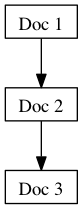
\includegraphics{code/ex15/ex1.png}

Now when the query gets executes MongoDB will start from the top of the chain and check each document to see if it matches \texttt{a equals 5}. If it does match it will add it to the result set otherwise it will skip to the next document. This is what is known as a \texttt{table scan} in the database world. If you imagine the chain containing millions of documents you can see that this is not a very efficient way of querying data as we would have to check each document for each query meaning a lot of reading data from disk. Thus a better approach to searching is needed and this is where the concept of an index comes in.


\subsection{Index Magic%
  \label{index-magic}%
}

Now indexes are not truly magic and once you grasp the main concept you'll wonder why you never thought of them yourself. The main index used in MongoDB is what's called a BTree index (or more specifically a variation of a BTree+ index).

So let's get into what a BTree index is. In very short it's a way to keep a list of values in a sorted order that's a tree structure and not a chain. What do you mean you might ask. Well it's easier to illustrate than explain.

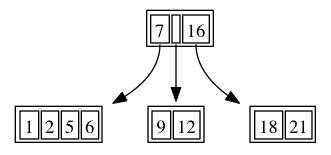
\includegraphics{code/ex15/ex2.png}

The tree above is an \texttt{index} for the field \texttt{a} in the documents above. Notice how it's a tree structure, instead of a chained list of documents. Each level of the tree contains a set of id's that correspond to a value that is stored in the \texttt{a} field in a document. So say we need to find the document with the value \texttt{a equals 5}. We grab the top node where we find the the first value to be \texttt{7}. We know our value is less than \texttt{7} so we decent into the left node of the tree and scan from left to right until we find the value \texttt{5} and we can now return the correct document. So instead of having to scan all documents we can short-cut our search because we have split the search \texttt{space} into smaller chunks of data to search through. So in this case given that we know that \texttt{a is less than 7} we only need to search through the documents that are \texttt{larger than 0 and less than 7} which are all contained in the left lower node.

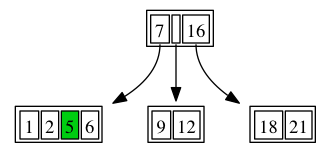
\includegraphics{code/ex15/ex3.png}

The main benefit comes from when our collections of documents grow very big as it allows MongoDB to limit the number of documents it needs to search through to find the correct matches to the query, thus speeding up the search massively compared to searching through all of the documents.

An index like this lets us look up a document by an indexed value very quickly but it also lets us do what is called a \texttt{ranged query}. A \texttt{ranged query} is a query that looks like this in mongodb \texttt{\{a:\{\$gt:0, \$lt:10\}\}}. This looks for all documents where \texttt{a is greater than 0 and less than 10}. Because of the way the Btree index is structured it helps us limit the amount of documents we need to search as as can see from the first node that we only have to search the leftmost and middle node for all values that are less than 10. So we only need to search the results

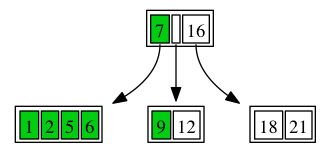
\includegraphics{code/ex15/ex4.png}

This is of course a very oversimplified way of explaining the way an index works but safe to say is that it allows you to search more efficiently for a value.

The last item we will cover is what's called a \texttt{compound index} and a beneficial side effect of \texttt{compound indexes} called \texttt{covered indexes}.


\subsection{Compound indexes%
  \label{compound-indexes}%
}

Besides support a single value index MongoDB also supports what's called a \texttt{compound ~index}. This type of index is made up of multiple values. Let's take an example of documents that look like this.
%
\begin{quote}{\ttfamily \raggedright \noindent
\DUrole{p}{\{}~\\
~~\DUrole{nx}{pid}\DUrole{o}{:}~\DUrole{mi}{1}\DUrole{p}{,}~\\
~~\DUrole{nx}{name}\DUrole{o}{:}~\DUrole{s1}{'Steve'}\DUrole{p}{,}~\\
~~\DUrole{nx}{salary}\DUrole{o}{:}~\DUrole{mi}{10000}~\\
\DUrole{p}{\}}~\\
~\\
\DUrole{p}{\{}~\\
~~\DUrole{nx}{pid}\DUrole{o}{:}~\DUrole{mi}{2}\DUrole{p}{,}~\\
~~\DUrole{nx}{name}\DUrole{o}{:}~\DUrole{s1}{'John'}\DUrole{p}{,}~\\
~~\DUrole{nx}{salary}\DUrole{o}{:}~\DUrole{mi}{12000}~\\
\DUrole{p}{\}}~\\
~\\
\DUrole{p}{\{}~\\
~~\DUrole{nx}{pid}\DUrole{o}{:}~\DUrole{mi}{7}\DUrole{p}{,}~\\
~~\DUrole{nx}{name}\DUrole{o}{:}~\DUrole{s1}{'Peter'}\DUrole{p}{,}~\\
~~\DUrole{nx}{salary}\DUrole{o}{:}~\DUrole{mi}{7000}~\\
\DUrole{p}{\}}~\\
~\\
\DUrole{p}{\{}~\\
~~\DUrole{nx}{pid}\DUrole{o}{:}~\DUrole{mi}{18}\DUrole{p}{,}~\\
~~\DUrole{nx}{name}\DUrole{o}{:}~\DUrole{s1}{'Arnold'}\DUrole{p}{,}~\\
~~\DUrole{nx}{salary}\DUrole{o}{:}~\DUrole{mi}{32000}~\\
\DUrole{p}{\}}~\\
~\\
\DUrole{p}{\{}~\\
~~\DUrole{nx}{pid}\DUrole{o}{:}~\DUrole{mi}{23}\DUrole{p}{,}~\\
~~\DUrole{nx}{name}\DUrole{o}{:}~\DUrole{s1}{'Gandalf'}\DUrole{p}{,}~\\
~~\DUrole{nx}{salary}\DUrole{o}{:}~\DUrole{mi}{34000}~\\
\DUrole{p}{\}}
}
\end{quote}

What if we want to efficiently search for documents where \texttt{pid is larger than 2 and the salary is less than 10000}. This is where a compound index comes in and allows us to do this efficiently. \texttt{Compound} means to combine and that what it is, an index that combines two or more fields. Let's look at an example of a compound index of \texttt{\{pid, salary, name\}}.

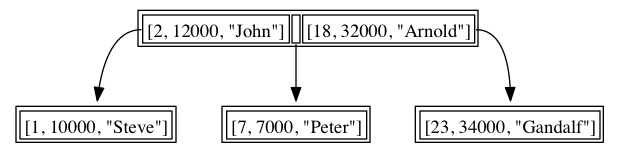
\includegraphics{code/ex15/ex5.png}

Now let's run our query against it. The first part of the query is the pid factor, so let's locate all the \texttt{pids larger than 2}

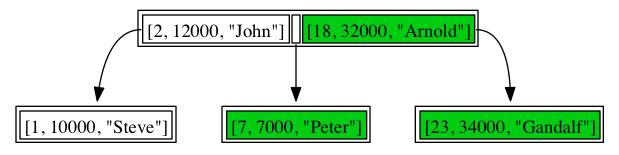
\includegraphics{code/ex15/ex6.png}

As you can see we have identified 3 nodes (colored green) that fulfill the the criteria of \texttt{pid larger than 2}. It's time to apply the second criteria to this new sub tree of results. Inside of the green nodes we locate the ones where \texttt{salary is less than 10000}

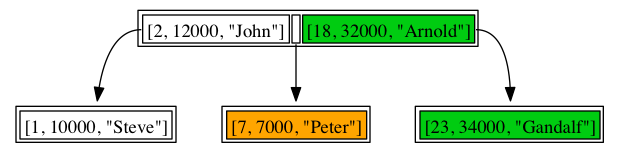
\includegraphics{code/ex15/ex7.png}

This is awesome, we can use a single index to narrow down the number of documents we need to search to locate the values in the query even if the query covers two or more fields. This brings us to the last aspect of compound indexes, namely \texttt{covered indexes}. Given that the data for \texttt{pid, salary, name} is already in the index we can retrieve the data directly from the index if the query only requires the fields in the index to be returned. This means we will not have to load the actual documents into memory to satisfy a query.

This covers the basics of how indexes work. We have not covered geo indexes or text indexes here on purpose as we will cover them in future exercises. Hopefully this introduction will be enough for you to grasp why indexes are one of the most important aspects of MongoDB and that they are vital to get maximum performance out your queries.


\section{Exercise 16: Basic Indexes in MongoDB%
  \label{exercise-16-basic-indexes-in-mongodb}%
}

In this exercise we will focus on the basics of creating indexes for MongoDB, using them and understanding how our queries use indexes. To kick off let's insert some documents into a database and create an index on the field salary.

\begin{Verbatim}[commandchars=\\\{\}]
\PY{k+kd}{var} \PY{n+nx}{mongodb} \PY{o}{=} \PY{n+nx}{require}\PY{p}{(}\PY{l+s+s1}{'mongodb'}\PY{p}{)}
  \PY{p}{,} \PY{n+nx}{MongoClient} \PY{o}{=} \PY{n+nx}{mongodb}\PY{p}{.}\PY{n+nx}{MongoClient}\PY{p}{;}

\PY{n+nx}{MongoClient}\PY{p}{.}\PY{n+nx}{connect}\PY{p}{(}\PY{l+s+s2}{"mongodb://localhost:27017/test"}\PY{p}{,} \PY{k+kd}{function}\PY{p}{(}\PY{n+nx}{err}\PY{p}{,} \PY{n+nx}{db}\PY{p}{)} \PY{p}{\PYZob{}}
  \PY{k}{if}\PY{p}{(}\PY{n+nx}{err}\PY{p}{)} \PY{p}{\PYZob{}}
    \PY{n+nx}{console}\PY{p}{.}\PY{n+nx}{log}\PY{p}{(}\PY{l+s+s2}{"failed to connect to the database"}\PY{p}{)}\PY{p}{;}
  \PY{p}{\PYZcb{}} \PY{k}{else} \PY{p}{\PYZob{}}
    \PY{n+nx}{console}\PY{p}{.}\PY{n+nx}{log}\PY{p}{(}\PY{l+s+s2}{"connected to database"}\PY{p}{)}\PY{p}{;}
  \PY{p}{\PYZcb{}}

  \PY{k+kd}{var} \PY{n+nx}{documents} \PY{o}{=} \PY{p}{[}
    \PY{p}{\PYZob{}}
      \PY{n+nx}{pid}\PY{o}{:} \PY{l+m+mi}{1}\PY{p}{,}
      \PY{n+nx}{name}\PY{o}{:} \PY{l+s+s1}{'Steve'}\PY{p}{,}
      \PY{n+nx}{salary}\PY{o}{:} \PY{l+m+mi}{10000}
    \PY{p}{\PYZcb{}}\PY{p}{,}
    \PY{p}{\PYZob{}}
      \PY{n+nx}{pid}\PY{o}{:} \PY{l+m+mi}{2}\PY{p}{,}
      \PY{n+nx}{name}\PY{o}{:} \PY{l+s+s1}{'John'}\PY{p}{,}
      \PY{n+nx}{salary}\PY{o}{:} \PY{l+m+mi}{12000}
    \PY{p}{\PYZcb{}}\PY{p}{,}
    \PY{p}{\PYZob{}}
      \PY{n+nx}{pid}\PY{o}{:} \PY{l+m+mi}{7}\PY{p}{,}
      \PY{n+nx}{name}\PY{o}{:} \PY{l+s+s1}{'Peter'}\PY{p}{,}
      \PY{n+nx}{salary}\PY{o}{:} \PY{l+m+mi}{7000}
    \PY{p}{\PYZcb{}}\PY{p}{,}
    \PY{p}{\PYZob{}}
      \PY{n+nx}{pid}\PY{o}{:} \PY{l+m+mi}{18}\PY{p}{,}
      \PY{n+nx}{name}\PY{o}{:} \PY{l+s+s1}{'Arnold'}\PY{p}{,}
      \PY{n+nx}{salary}\PY{o}{:} \PY{l+m+mi}{32000}
    \PY{p}{\PYZcb{}}\PY{p}{,}
    \PY{p}{\PYZob{}}
      \PY{n+nx}{pid}\PY{o}{:} \PY{l+m+mi}{23}\PY{p}{,}
      \PY{n+nx}{name}\PY{o}{:} \PY{l+s+s1}{'Gandalf'}\PY{p}{,}
      \PY{n+nx}{salary}\PY{o}{:} \PY{l+m+mi}{34000}
    \PY{p}{\PYZcb{}}
  \PY{p}{]}\PY{p}{;}

  \PY{k+kd}{var} \PY{n+nx}{collection} \PY{o}{=} \PY{n+nx}{db}\PY{p}{.}\PY{n+nx}{collection}\PY{p}{(}\PY{l+s+s1}{'salaries'}\PY{p}{)}\PY{p}{;}
  \PY{n+nx}{collection}\PY{p}{.}\PY{n+nx}{remove}\PY{p}{(}\PY{k+kd}{function}\PY{p}{(}\PY{n+nx}{err}\PY{p}{,} \PY{n+nx}{result}\PY{p}{)} \PY{p}{\PYZob{}}

    \PY{n+nx}{collection}\PY{p}{.}\PY{n+nx}{insert}\PY{p}{(}\PY{n+nx}{documents}\PY{p}{,} \PY{k+kd}{function}\PY{p}{(}\PY{n+nx}{err}\PY{p}{,} \PY{n+nx}{result}\PY{p}{)} \PY{p}{\PYZob{}}
      \PY{k}{if}\PY{p}{(}\PY{n+nx}{err}\PY{p}{)} \PY{k}{throw} \PY{n+nx}{err}\PY{p}{;}
      \PY{n+nx}{console}\PY{p}{.}\PY{n+nx}{log}\PY{p}{(}\PY{l+s+s2}{"added salary documents"}\PY{p}{)}\PY{p}{;}

      \PY{n+nx}{collection}\PY{p}{.}\PY{n+nx}{ensureIndex}\PY{p}{(}\PY{p}{\PYZob{}}\PY{n+nx}{salary}\PY{o}{:}\PY{l+m+mi}{1}\PY{p}{\PYZcb{}}\PY{p}{,} \PY{k+kd}{function}\PY{p}{(}\PY{n+nx}{err}\PY{p}{,} \PY{n+nx}{index\PYZus{}name}\PY{p}{)} \PY{p}{\PYZob{}}

        \PY{n+nx}{collection}\PY{p}{.}\PY{n+nx}{find}\PY{p}{(}\PY{p}{\PYZob{}}\PY{n+nx}{salary}\PY{o}{:}\PY{l+m+mi}{7000}\PY{p}{\PYZcb{}}\PY{p}{)}\PY{p}{.}\PY{n+nx}{toArray}\PY{p}{(}\PY{k+kd}{function}\PY{p}{(}\PY{n+nx}{err}\PY{p}{,} \PY{n+nx}{docs}\PY{p}{)} \PY{p}{\PYZob{}}
          \PY{n+nx}{console}\PY{p}{.}\PY{n+nx}{log}\PY{p}{(}\PY{l+s+s2}{"documents"}\PY{p}{)}\PY{p}{;}
          \PY{n+nx}{console}\PY{p}{.}\PY{n+nx}{dir}\PY{p}{(}\PY{n+nx}{docs}\PY{p}{)}\PY{p}{;}
          \PY{n+nx}{db}\PY{p}{.}\PY{n+nx}{close}\PY{p}{(}\PY{p}{)}\PY{p}{;}
        \PY{p}{\PYZcb{}}\PY{p}{)}\PY{p}{;}
      \PY{p}{\PYZcb{}}\PY{p}{)}\PY{p}{;}
    \PY{p}{\PYZcb{}}\PY{p}{)}\PY{p}{;}
  \PY{p}{\PYZcb{}}\PY{p}{)}\PY{p}{;}
\PY{p}{\PYZcb{}}\PY{p}{)}\PY{p}{;}
\end{Verbatim}

Let's have a look at the new collection method we are using called \texttt{ensureIndex}. The call looks like.
%
\begin{quote}{\ttfamily \raggedright \noindent
\DUrole{nx}{collection}\DUrole{p}{.}\DUrole{nx}{ensureIndex}\DUrole{p}{(}\DUrole{p}{\{}\DUrole{nx}{salary}\DUrole{o}{:}\DUrole{mi}{1}\DUrole{p}{\},}~\DUrole{kd}{function}\DUrole{p}{(}\DUrole{nx}{err}\DUrole{p}{,}~\DUrole{nx}{index\_name}\DUrole{p}{)}~\DUrole{p}{\{}~\\
\DUrole{p}{\}}
}
\end{quote}

The \texttt{ensureIndex} method will only add the index if there is not an index already present. This lets you specify the index creation as part of your code to ensure that the specified index exists. A typical place to locate this code is at the boot up time of your application so the indexes are built before your application is ready to process incoming requests (if an web app).

The meat of the story is the \texttt{\{salary:1\}} index specifier. This tells MongoDB to build a \texttt{BTree index} over the field \texttt{salary} in all documents present in the collection. If you remember from the introduction on indexes this will create a tree structure allowing us to efficiently query the data. The next line is the actual query.
%
\begin{quote}{\ttfamily \raggedright \noindent
\DUrole{nx}{collection}\DUrole{p}{.}\DUrole{nx}{find}\DUrole{p}{(}\DUrole{p}{\{}\DUrole{nx}{salary}\DUrole{o}{:}\DUrole{mi}{7000}\DUrole{p}{\}).}\DUrole{nx}{toArray}\DUrole{p}{(}\DUrole{kd}{function}\DUrole{p}{(}\DUrole{nx}{err}\DUrole{p}{,}~\DUrole{nx}{docs}\DUrole{p}{)}~\DUrole{p}{\{}~\\
\DUrole{p}{\}}
}
\end{quote}

This will look for any documents where the \texttt{salary is equal to 7000} and the output after running the example is (\_id will vary).
%
\begin{quote}{\ttfamily \raggedright \noindent
\DUrole{go}{connected~to~database\\
added~salary~documents\\
documents\\
{[}~\{~pid:~7,\\
name:~'Peter',\\
salary:~7000,\\
\_id:~51811ee1746bbbc015000003~\}~{]}}
}
\end{quote}

But how can we know if a query is using an index ?. Actually you can do this both from the driver as well as the \texttt{mongo shell}. To be fair it's probably better to do it from the shell but let's cover what that would look like using the driver. The code below \texttt{requires} that the first example has been run first to populate the collection and create the index. Notice that we use a option for the \texttt{find} method called \texttt{explain}. This tells the server to return the \texttt{query plan} or the way it searched for data instead of the actual data for the query.

\begin{Verbatim}[commandchars=\\\{\}]
\PY{k+kd}{var} \PY{n+nx}{mongodb} \PY{o}{=} \PY{n+nx}{require}\PY{p}{(}\PY{l+s+s1}{'mongodb'}\PY{p}{)}
  \PY{p}{,} \PY{n+nx}{MongoClient} \PY{o}{=} \PY{n+nx}{mongodb}\PY{p}{.}\PY{n+nx}{MongoClient}\PY{p}{;}

\PY{n+nx}{MongoClient}\PY{p}{.}\PY{n+nx}{connect}\PY{p}{(}\PY{l+s+s2}{"mongodb://localhost:27017/test"}\PY{p}{,} \PY{k+kd}{function}\PY{p}{(}\PY{n+nx}{err}\PY{p}{,} \PY{n+nx}{db}\PY{p}{)} \PY{p}{\PYZob{}}
  \PY{k}{if}\PY{p}{(}\PY{n+nx}{err}\PY{p}{)} \PY{p}{\PYZob{}}
    \PY{n+nx}{console}\PY{p}{.}\PY{n+nx}{log}\PY{p}{(}\PY{l+s+s2}{"failed to connect to the database"}\PY{p}{)}\PY{p}{;}
  \PY{p}{\PYZcb{}} \PY{k}{else} \PY{p}{\PYZob{}}
    \PY{n+nx}{console}\PY{p}{.}\PY{n+nx}{log}\PY{p}{(}\PY{l+s+s2}{"connected to database"}\PY{p}{)}\PY{p}{;}
  \PY{p}{\PYZcb{}}
  \PY{k+kd}{var} \PY{n+nx}{collection} \PY{o}{=} \PY{n+nx}{db}\PY{p}{.}\PY{n+nx}{collection}\PY{p}{(}\PY{l+s+s1}{'salaries'}\PY{p}{)}\PY{p}{;}
  \PY{n+nx}{collection}\PY{p}{.}\PY{n+nx}{find}\PY{p}{(}\PY{p}{\PYZob{}}\PY{n+nx}{salary}\PY{o}{:}\PY{l+m+mi}{7000}\PY{p}{\PYZcb{}}\PY{p}{,} \PY{p}{\PYZob{}}\PY{n+nx}{explain}\PY{o}{:}\PY{k+kc}{true}\PY{p}{\PYZcb{}}\PY{p}{)}\PY{p}{.}\PY{n+nx}{toArray}\PY{p}{(}\PY{k+kd}{function}\PY{p}{(}\PY{n+nx}{err}\PY{p}{,} \PY{n+nx}{docs}\PY{p}{)} \PY{p}{\PYZob{}}
    \PY{n+nx}{console}\PY{p}{.}\PY{n+nx}{log}\PY{p}{(}\PY{l+s+s2}{"documents"}\PY{p}{)}\PY{p}{;}
    \PY{n+nx}{console}\PY{p}{.}\PY{n+nx}{dir}\PY{p}{(}\PY{n+nx}{docs}\PY{p}{)}\PY{p}{;}
    \PY{n+nx}{db}\PY{p}{.}\PY{n+nx}{close}\PY{p}{(}\PY{p}{)}\PY{p}{;}
  \PY{p}{\PYZcb{}}\PY{p}{)}\PY{p}{;}
\PY{p}{\PYZcb{}}\PY{p}{)}\PY{p}{;}
\end{Verbatim}

After running the example you'll see the following
%
\begin{quote}{\ttfamily \raggedright \noindent
\DUrole{go}{connected~to~database\\
documents\\
{[}~\{~cursor:~'BtreeCursor~salary\_1',\\
~~~~isMultiKey:~false,\\
~~~~n:~1,\\
~~~~nscannedObjects:~1,\\
~~~~nscanned:~1,\\
~~~~nscannedObjectsAllPlans:~1,\\
~~~~nscannedAllPlans:~1,\\
~~~~scanAndOrder:~false,\\
~~~~indexOnly:~false,\\
~~~~nYields:~0,\\
~~~~nChunkSkips:~0,\\
~~~~millis:~0,\\
~~~~indexBounds:~\{~salary:~{[}Object{]}~\},\\
~~~~allPlans:~{[}~{[}Object{]}~{]},\\
~~~~oldPlan:~\{~cursor:~'BtreeCursor~salary\_1',~indexBounds:~{[}Object{]}~\},\\
~~~~server:~'localhost:27017'~\}~{]}}
}
\end{quote}

This can be done more simply from the \texttt{mongo} shell executing the following commands.
%
\begin{quote}{\ttfamily \raggedright \noindent
\DUrole{go}{mongo\\
MongoDB~shell~version:~2.4.3\\
connecting~to:~test\\
}\DUrole{gp}{>}~db.salaries.find\DUrole{o}{(\{}salary:7000\DUrole{o}{\})}.explain\DUrole{o}{(}\DUrole{nb}{true}\DUrole{o}{)}~\\
\DUrole{go}{\{\\
~~"cursor"~:~"BtreeCursor~salary\_1",\\
~~"isMultiKey"~:~false,\\
~~"n"~:~1,\\
~~"nscannedObjects"~:~1,\\
~~"nscanned"~:~1,\\
~~"nscannedObjectsAllPlans"~:~1,\\
~~"nscannedAllPlans"~:~1,\\
~~"scanAndOrder"~:~false,\\
~~"indexOnly"~:~false,\\
~~"nYields"~:~0,\\
~~"nChunkSkips"~:~0,\\
~~"millis"~:~0,\\
~~"indexBounds"~:~\{\\
~~~~"salary"~:~{[}\\
~~~~~~{[}\\
~~~~~~~~7000,\\
~~~~~~~~7000\\
~~~~~~{]}\\
~~~~{]}\\
~~\},\\
~~"allPlans"~:~{[}\\
~~~~~~\{\\
~~~~~~~~"cursor"~:~"BtreeCursor~salary\_1",\\
~~~~~~~~"n"~:~1,\\
~~~~~~~~"nscannedObjects"~:~1,\\
~~~~~~~~"nscanned"~:~1,\\
~~~~~~~~"indexBounds"~:~\{\\
~~~~~~~~~~"salary"~:~{[}\\
~~~~~~~~~~~~{[}\\
~~~~~~~~~~~~~~7000,\\
~~~~~~~~~~~~~~7000\\
~~~~~~~~~~~~{]}\\
~~~~~~~~~~{]}\\
~~~~~~~~\}\\
~~~~~~\}\\
~~~~{]},\\
~~~~"oldPlan"~:~\{\\
~~~~~~"cursor"~:~"BtreeCursor~salary\_1",\\
~~~~~~"indexBounds"~:~\{\\
~~~~~~~~"salary"~:~{[}\\
~~~~~~~~~~{[}\\
~~~~~~~~~~~~7000,\\
~~~~~~~~~~~~7000\\
~~~~~~~~~~{]}\\
~~~~~~~~{]}\\
~~~~~~\}\\
~~~~\},\\
~~"server"~:~"localhost:27017"\\
\}\\
}\DUrole{gp}{>}~\DUrole{nb}{exit}~\\
\DUrole{go}{bye}
}
\end{quote}

I personally prefer to use the \texttt{mongo} shell to \texttt{explain} queries as it does not require me to write additional code.

So let's pick apart what the explain document actually means and how it relates to the usage of the documents.

\setlength{\DUtablewidth}{\linewidth}
\begin{longtable*}[c]{|p{0.133\DUtablewidth}|p{0.117\DUtablewidth}|p{0.694\DUtablewidth}|}
\hline
\textbf{%
Field
} & \textbf{%
Value
} & \textbf{%
Description
} \\
\hline
\endfirsthead
\hline
\textbf{%
Field
} & \textbf{%
Value
} & \textbf{%
Description
} \\
\hline
\endhead
\multicolumn{3}{c}{\hfill ... continued on next page} \\
\endfoot
\endlastfoot

cursor
 & 
BtreeCursor salary\_1
 & 
Tells us what kind of cursor was used for the query. In this case it was a BtreeCursor which means it used the \texttt{salary} index.
 \\
\hline

isMultiKey
 & 
false
 & 
If true it tells us that one of the fields in the index is an array of values.
 \\
\hline

n
 & 
1
 & 
The number of documents that matches the query.
 \\
\hline

nscannedObjects
 & 
1
 & 
The number of documents scanned during the query
 \\
\hline

nscanned
 & 
1
 & 
The number of documents + index entries scanned during the query.
 \\
\hline

nscannedObjectsAllPlans
 & 
1
 & 
The total number of documents scanned for all query plans;
 \\
\hline

nscannedAllPlans
 & 
1
 & 
The total number of documents + index entries scanned across all query plans.
 \\
\hline

scanAndOrder
 & 
false
 & 
Is true if an index cannot be used to order the documents returned.
 \\
\hline

indexOnly
 & 
false
 & 
Is true if the query can be answered using only the data stored in the index.
 \\
\hline

nYields
 & 
0
 & 
The number of times MongoDB let somebody else perform work while executing the query.
 \\
\hline

nChunkSkips
 & 
0
 & 
Advanced field for sharding, reflects the number of chunks skipped during the search because chunks were being migrated.
 \\
\hline

millis
 & 
0
 & 
The miliseconds it took to execute the query.
 \\
\hline

indexBounds
 & 
salary:{[}{[}7000,7000{]}{]}
 & 
Contains what field in the index satisfied the query and what range of the index was used to locate the documents.
 \\
\hline

allPlans
 & 
...
 & 
Contains a list of all the query plans MongoDB tried when executing the query
 \\
\hline

oldPlan
 & 
...
 & 
Contains the last query plan used for this query (MongoDB caches the most efficient query plan and reuses it)
 \\
\hline

``server''
 & 
localhost:27017
 & 
Server the query was run against
 \\
\hline
\end{longtable*}

As you can see it's quite a lot of information. The easiest way to understand how to read it is to contrast the information above with a query that does not use an index.
%
\begin{quote}{\ttfamily \raggedright \noindent
\DUrole{go}{~~mongo\\
~~MongoDB~shell~version:~2.4.3\\
~~connecting~to:~test\\
~~>~db.salaries.find(\{name:~"Steve"\}).explain(true)\\
~~\{\\
~~~~"cursor"~:~"BasicCursor",\\
~~~~"isMultiKey"~:~false,\\
~~~~"n"~:~1,\\
~~~~"nscannedObjects"~:~5,\\
~~~~"nscanned"~:~5,\\
~~~~"nscannedObjectsAllPlans"~:~5,\\
~~~~"nscannedAllPlans"~:~5,\\
~~~~"scanAndOrder"~:~false,\\
~~~~"indexOnly"~:~false,\\
~~~~"nYields"~:~0,\\
~~~~"nChunkSkips"~:~0,\\
~~~~"millis"~:~0,\\
~~~~"indexBounds"~:~\{\\
~\\
~~~~\},\\
~~~~"allPlans"~:~{[}\\
~~~~~~\{\\
~~~~~~~~"cursor"~:~"BasicCursor",\\
~~~~~~~~"n"~:~1,\\
~~~~~~~~"nscannedObjects"~:~5,\\
~~~~~~~~"nscanned"~:~5,\\
~~~~~~~~"indexBounds"~:~\{\\
~\\
~~~~~~~~\}\\
~~~~~~\}\\
~~~~{]},\\
~~~~"server"~:~"localhost:27017"\\
~~\}\\
~~quit\\
~~bye\\
~\\
Let's~look~at~the~two~side~by~side.}
}
\end{quote}

\setlength{\DUtablewidth}{\linewidth}
\begin{longtable*}[c]{|p{0.331\DUtablewidth}|p{0.296\DUtablewidth}|p{0.272\DUtablewidth}|}
\hline
\textbf{%
Field
} & \textbf{%
Value
} & \textbf{%
Value
} \\
\hline
\endfirsthead
\hline
\textbf{%
Field
} & \textbf{%
Value
} & \textbf{%
Value
} \\
\hline
\endhead
\multicolumn{3}{c}{\hfill ... continued on next page} \\
\endfoot
\endlastfoot

\texttt{cursor}
 & 
\texttt{BtreeCursor salary\_1}
 & 
\texttt{BasicCursor}
 \\
\hline

isMultiKey
 & 
false
 & 
false
 \\
\hline

n
 & 
1
 & 
1
 \\
\hline

\texttt{nscannedObjects}
 & 
\texttt{1}
 & 
\texttt{5}
 \\
\hline

\texttt{nscanned}
 & 
\texttt{1}
 & 
\texttt{5}
 \\
\hline

\texttt{nscannedObjectsAllPlans}
 & 
\texttt{1}
 & 
\texttt{5}
 \\
\hline

\texttt{nscannedAllPlans}
 & 
\texttt{1}
 & 
\texttt{5}
 \\
\hline

scanAndOrder
 & 
false
 & 
false
 \\
\hline

indexOnly
 & 
false
 & 
false
 \\
\hline

nYields
 & 
0
 & 
0
 \\
\hline

nChunkSkips
 & 
0
 & 
0
 \\
\hline

millis
 & 
0
 & 
0
 \\
\hline

indexBounds
 & 
salary:{[}{[}7000,7000{]}{]}
 & 
\{\}
 \\
\hline

allPlans
 & 
...
 & 
...
 \\
\hline

oldPlan
 & 
...
 & 
...
 \\
\hline

``server''
 & 
localhost:27017
 & 
localhost:27017
 \\
\hline
\end{longtable*}

Notice how the \texttt{cursor} field says \texttt{BasicCursor} instead off \texttt{BtreeCursor}. This tells us that the query did not use an index and had to go through all of the documents in the collection to satisfy the query. This directly leads to \texttt{nscannedObjects}, \texttt{nscanned}, \texttt{nscannedObjectsAllPlans} and \texttt{nscannedAllPlans} being \texttt{5} as there are \texttt{5} documents in the collection. Also as MongoDB did not use an index for the query the \texttt{indexBound} is empty as we could not locate a boundary for the query (remember how the Btree is laid out, a boundary is the set of tree node ranges needed to satisfy the query)

Imagine that there was \texttt{hundreds of thousands} of documents in the collection instead of just 5. A query looking up a name would require each query to scan through all of the documents to locate matching documents. This would very quickly become unsustainable as the slowness of the query would be compounded by many of them happening in parallel. Even worse since MongoDB would have to load every document into it could cause excessive swapping out of memory to disk (moving documents out of RAM to make space for the ones we need to scan) making the queries even slower and limiting the performance of our application. This is why we need to make sure we always use indexes and even more so if the collection of documents is very large. Cool that covers the basics of understanding how we can create a simple index and how we can investigate if a query is using it correctly or not. Next exercise we will build a ton of different indexes and see how they work and perform.

\DUadmonition[note]{
\DUtitle[note]{Note}

In development I tend to use an option for \texttt{mongod} that allows me to catch queries that don't use an index. When you start up the \texttt{mongod} server add the option \texttt{-{}-notablescan} to the \texttt{mongod} command line. If you now attempt to run a query that does not use an index MongoDb will throw an error \texttt{\{"\$err" : "table scans not allowed:test.salaries", "code" : 10111 \}}
}


\section{Exercise 17: Index Katas%
  \label{exercise-17-index-katas}%
}

Let's do a bunch of index Katas to get used to how indexes work in MongoDB. A Kata is a form or pattern. Let's start off with the single value index.


\subsection{Single Value Index%
  \label{single-value-index}%
}

Given the documents inserted into the database \texttt{test} and collection \texttt{users}.
%
\begin{quote}{\ttfamily \raggedright \noindent
\DUrole{p}{\{}~\\
~~\DUrole{nx}{pid}\DUrole{o}{:}~\DUrole{mi}{1}\DUrole{p}{,}~\\
~~\DUrole{nx}{name}\DUrole{o}{:}~\DUrole{s1}{'Steve'}\DUrole{p}{,}~\\
~~\DUrole{nx}{salary}\DUrole{o}{:}~\DUrole{mi}{10000}~\\
\DUrole{p}{\}}~\\
~\\
\DUrole{p}{\{}~\\
~~\DUrole{nx}{pid}\DUrole{o}{:}~\DUrole{mi}{2}\DUrole{p}{,}~\\
~~\DUrole{nx}{name}\DUrole{o}{:}~\DUrole{s1}{'John'}\DUrole{p}{,}~\\
~~\DUrole{nx}{salary}\DUrole{o}{:}~\DUrole{mi}{12000}~\\
\DUrole{p}{\}}~\\
~\\
\DUrole{p}{\{}~\\
~~\DUrole{nx}{pid}\DUrole{o}{:}~\DUrole{mi}{7}\DUrole{p}{,}~\\
~~\DUrole{nx}{name}\DUrole{o}{:}~\DUrole{s1}{'Peter'}\DUrole{p}{,}~\\
~~\DUrole{nx}{salary}\DUrole{o}{:}~\DUrole{mi}{7000}~\\
\DUrole{p}{\}}~\\
~\\
\DUrole{p}{\{}~\\
~~\DUrole{nx}{pid}\DUrole{o}{:}~\DUrole{mi}{18}\DUrole{p}{,}~\\
~~\DUrole{nx}{name}\DUrole{o}{:}~\DUrole{s1}{'Arnold'}\DUrole{p}{,}~\\
~~\DUrole{nx}{salary}\DUrole{o}{:}~\DUrole{mi}{32000}~\\
\DUrole{p}{\}}
}
\end{quote}

We want to create an index on the \texttt{salary} field so we can perform two queries using the index. The first one is \texttt{locate all users with the salary 10000} and the second one is the query \texttt{locate all users that have a salary less then 30000 but larger than 8000}.

Let's create the index using either the driver
%
\begin{quote}{\ttfamily \raggedright \noindent
\DUrole{nx}{db}\DUrole{p}{.}\DUrole{nx}{collection}\DUrole{p}{(}\DUrole{s1}{'users'}\DUrole{p}{).}\DUrole{nx}{ensureIndex}\DUrole{p}{(}\DUrole{p}{\{}\DUrole{nx}{salary}\DUrole{o}{:}\DUrole{mi}{1}\DUrole{p}{\},}~\DUrole{kd}{function}\DUrole{p}{(}\DUrole{nx}{err}\DUrole{p}{,}~\DUrole{nx}{result}\DUrole{p}{)}~\DUrole{p}{\{}\DUrole{p}{\});}
}
\end{quote}

or the console
%
\begin{quote}{\ttfamily \raggedright \noindent
\DUrole{gp}{>}~use~\DUrole{nb}{test\\
}\DUrole{gp}{>}\DUrole{nb}{~}db.users.ensureIndex\DUrole{o}{(\{}salary:1\DUrole{o}{\})}
}
\end{quote}

Let's execute the queries mentioned above using the \texttt{console} and have a look at the resulting explain results.

First the \texttt{locate all users with the salary 10000} query
%
\begin{quote}{\ttfamily \raggedright \noindent
\DUrole{gp}{>}~use~\DUrole{nb}{test\\
}\DUrole{gp}{>}\DUrole{nb}{~}db.users.find\DUrole{o}{(\{}salary:10000\DUrole{o}{\})}.explain\DUrole{o}{()}~\\
\DUrole{go}{\{\\
~~"cursor"~:~"BtreeCursor~salary\_1",\\
~~"isMultiKey"~:~false,\\
~~"n"~:~1,\\
~~"nscannedObjects"~:~1,\\
~~"nscanned"~:~1,\\
~~"nscannedObjectsAllPlans"~:~1,\\
~~"nscannedAllPlans"~:~1,\\
~~"scanAndOrder"~:~false,\\
~~"indexOnly"~:~false,\\
~~"nYields"~:~0,\\
~~"nChunkSkips"~:~0,\\
~~"millis"~:~0,\\
~~"indexBounds"~:~\{\\
~~~~"salary"~:~{[}\\
~~~~~~{[}\\
~~~~~~~~10000,\\
~~~~~~~~10000\\
~~~~~~{]}\\
~~~~{]}\\
~~\},\\
~~"server"~:~"localhost:27017"\\
\}}
}
\end{quote}

and then the \texttt{locate all users that have a salary less then 30000 but larger than 8000} query.
%
\begin{quote}{\ttfamily \raggedright \noindent
\DUrole{gp}{>}~use~\DUrole{nb}{test\\
}\DUrole{gp}{>}\DUrole{nb}{~}db.users.find\DUrole{o}{(\{}salary:\DUrole{o}{\{}\DUrole{nv}{\$lt}:~30000,~\DUrole{nv}{\$gt}:~8000\DUrole{o}{\}\})}.explain\DUrole{o}{()}~\\
\DUrole{go}{\{\\
~~"cursor"~:~"BtreeCursor~salary\_1",\\
~~"isMultiKey"~:~false,\\
~~"n"~:~2,\\
~~"nscannedObjects"~:~2,\\
~~"nscanned"~:~2,\\
~~"nscannedObjectsAllPlans"~:~2,\\
~~"nscannedAllPlans"~:~2,\\
~~"scanAndOrder"~:~false,\\
~~"indexOnly"~:~false,\\
~~"nYields"~:~0,\\
~~"nChunkSkips"~:~0,\\
~~"millis"~:~0,\\
~~"indexBounds"~:~\{\\
~~~~"salary"~:~{[}\\
~~~~~~{[}\\
~~~~~~~~8000,\\
~~~~~~~~30000\\
~~~~~~{]}\\
~~~~{]}\\
~~\},\\
~~"server"~:~"localhost:27017"\\
\}}
}
\end{quote}

As you notice we are explicitly making you look the \texttt{explains} for the queries. We are trying to impart the importance of understanding how you queries use indexes as it's a prime factor in getting the best performance out of all databases. Going forward we will only touch on the explain part when it expands the understanding of how indexes work. Let's move on to a single index with sorting.


\subsection{Single Value Index With Sorting%
  \label{single-value-index-with-sorting}%
}

Let's play with sorting and using an index. For this we need a bigger set of data to play with. Let's generate some using the \texttt{mongo} shell. Remember it's a JavaScript \texttt{repl} so we can script it in JavaScript.
%
\begin{quote}{\ttfamily \raggedright \noindent
\DUrole{gp}{>}~use~\DUrole{nb}{test\\
}\DUrole{gp}{>}\DUrole{nb}{~}\DUrole{k}{for}\DUrole{o}{(}var~\DUrole{nv}{i}~\DUrole{o}{=}~0;~i~<~10000;~i++\DUrole{o}{)}~db.sorting.insert\DUrole{o}{(\{}a:i,~b:\DUrole{o}{(}10000~-~i\DUrole{o}{)\})}
}
\end{quote}

This will generate \texttt{10000} documents with an a field \texttt{a} that increases for each insert (as well as an increasing \texttt{b} field).

\DUadmonition[note]{
\DUtitle[note]{Note}

When we create an index we have to specify either \texttt{-1} or \texttt{1}. This is the ordering of the data in the index. \texttt{-1} means in \texttt{descending} (4, 3, 2, 1), while \texttt{1} means \texttt{ascending} sort order (1, 2, 3, 4). This impacts how data is scanned in indexes and optimally you should always create the index in the \texttt{sort} order that will used in most of the queries to make them as efficient as possible.
}

Now let's add an index to this field.
%
\begin{quote}{\ttfamily \raggedright \noindent
\DUrole{gp}{>}~use~\DUrole{nb}{test\\
}\DUrole{gp}{>}\DUrole{nb}{~}db.sorting.ensureIndex\DUrole{o}{(\{}a:1\DUrole{o}{\})}
}
\end{quote}

The index can be created in the following way with the driver.
%
\begin{quote}{\ttfamily \raggedright \noindent
\DUrole{nx}{db}\DUrole{p}{.}\DUrole{nx}{collection}\DUrole{p}{(}\DUrole{s1}{'employees'}\DUrole{p}{).}\DUrole{nx}{ensureIndex}\DUrole{p}{(}\DUrole{p}{\{}\DUrole{nx}{a}\DUrole{o}{:}\DUrole{mi}{1}\DUrole{p}{\},}~\DUrole{kd}{function}\DUrole{p}{(}\DUrole{nx}{err}\DUrole{p}{,}~\DUrole{nx}{result}\DUrole{p}{)}~\DUrole{p}{\{}\DUrole{p}{\});}
}
\end{quote}

Let's look at how it works when we are using a sort.
%
\begin{quote}{\ttfamily \raggedright \noindent
\DUrole{gp}{>}~use~\DUrole{nb}{test\\
}\DUrole{gp}{>}\DUrole{nb}{~}db.sorting.find\DUrole{o}{(\{}a:~\DUrole{o}{\{}\DUrole{nv}{\$lt}:5000,~\DUrole{nv}{\$gt}:~1000\DUrole{o}{\}\})}.sort\DUrole{o}{(\{}a:1\DUrole{o}{\})}.explain\DUrole{o}{()}~\\
\DUrole{go}{\{\\
~~"cursor"~:~"BtreeCursor~a\_1",\\
~~"isMultiKey"~:~false,\\
~~"n"~:~3999,\\
~~"nscannedObjects"~:~3999,\\
~~"nscanned"~:~3999,\\
~~"nscannedObjectsAllPlans"~:~3999,\\
~~"nscannedAllPlans"~:~3999,\\
~~"scanAndOrder"~:~false,\\
~~"indexOnly"~:~false,\\
~~"nYields"~:~0,\\
~~"nChunkSkips"~:~0,\\
~~"millis"~:~6,\\
~~"indexBounds"~:~\{\\
~~~~"a"~:~{[}\\
~~~~~~{[}\\
~~~~~~~~1000,\\
~~~~~~~~5000\\
~~~~~~{]}\\
~~~~{]}\\
~~\},\\
~~"server"~:~"localhost:27017"\\
\}}
}
\end{quote}

Contrast that to
%
\begin{quote}{\ttfamily \raggedright \noindent
\DUrole{gp}{>}~use~\DUrole{nb}{test\\
}\DUrole{gp}{>}\DUrole{nb}{~}db.sorting.find\DUrole{o}{(\{}a:~\DUrole{o}{\{}\DUrole{nv}{\$lt}:5000,~\DUrole{nv}{\$gt}:~1000\DUrole{o}{\}\})}.sort\DUrole{o}{(\{}a:-1\DUrole{o}{\})}.explain\DUrole{o}{()}~\\
\DUrole{go}{\{\\
~~"cursor"~:~"BtreeCursor~a\_1~reverse",\\
~~"isMultiKey"~:~false,\\
~~"n"~:~3999,\\
~~"nscannedObjects"~:~3999,\\
~~"nscanned"~:~3999,\\
~~"nscannedObjectsAllPlans"~:~3999,\\
~~"nscannedAllPlans"~:~3999,\\
~~"scanAndOrder"~:~false,\\
~~"indexOnly"~:~false,\\
~~"nYields"~:~0,\\
~~"nChunkSkips"~:~0,\\
~~"millis"~:~6,\\
~~"indexBounds"~:~\{\\
~~~~"a"~:~{[}\\
~~~~~~{[}\\
~~~~~~~~5000,\\
~~~~~~~~1000\\
~~~~~~{]}\\
~~~~{]}\\
~~\},\\
~~"server"~:~"localhost:27017"\\
\}}
}
\end{quote}

Notice how \texttt{cursor} says \texttt{BtreeCursor a\_1 reverse} instead off \texttt{BtreeCursor a\_1}. This is because \texttt{MongoDB} was able to use the index to sort the values by traversing the \texttt{index} tree in the \texttt{reverse} order.

But what if we sort on the field \texttt{b} instead. Let's try it.
%
\begin{quote}{\ttfamily \raggedright \noindent
\DUrole{gp}{>}~use~\DUrole{nb}{test\\
}\DUrole{gp}{>}\DUrole{nb}{~}db.sorting.find\DUrole{o}{(\{}a:~\DUrole{o}{\{}\DUrole{nv}{\$lt}:5000,~\DUrole{nv}{\$gt}:~1000\DUrole{o}{\}\})}.sort\DUrole{o}{(\{}b:1\DUrole{o}{\})}.explain\DUrole{o}{()}~\\
\DUrole{go}{\{\\
~~"cursor"~:~"BtreeCursor~a\_1",\\
~~"isMultiKey"~:~false,\\
~~"n"~:~3999,\\
~~"nscannedObjects"~:~3999,\\
~~"nscanned"~:~3999,\\
~~"nscannedObjectsAllPlans"~:~4100,\\
~~"nscannedAllPlans"~:~4100,\\
~~"scanAndOrder"~:~true,\\
~~"indexOnly"~:~false,\\
~~"nYields"~:~0,\\
~~"nChunkSkips"~:~0,\\
~~"millis"~:~22,\\
~~"indexBounds"~:~\{\\
~~~~"a"~:~{[}\\
~~~~~~{[}\\
~~~~~~~~1000,\\
~~~~~~~~5000\\
~~~~~~{]}\\
~~~~{]}\\
~~\},\\
~~"server"~:~"localhost:27017"\\
\}}
}
\end{quote}

Let's look at the field here \texttt{scanAndOrder}. \texttt{scanAndOrder} is defined as \texttt{Is true if an index cannot be used to order the documents returned.}. In the cases where we are using \texttt{a} for sorting this is set to \texttt{false} as the index can be used for the sorting. But in the case of using \texttt{b} for sorting MongoDB cannot use the \texttt{a} index for sorting so it uses it to retrieve all the matching documents by the query and then sorts them by \texttt{b} in memory.
%
\begin{description}
\item[{NOTE::}] \leavevmode 
At the moment MongoDB can only use a single index for a query and sort, this will change in the future to allow multiple indexes to be used in a query and sort scenario.

\end{description}


\subsection{Compound That Index%
  \label{compound-that-index}%
}

So we've looked at single value indexes. But what if we want to search by \texttt{a} as well as \texttt{b} and also a combination of the two. This is where \texttt{compound indexes} come in. A \texttt{compound index} is an index built up of one or fields. Let's use the data from the previous example to play around with the implications for search. But first let's drop the existing indexes and then create the compound index \texttt{\{a:1, b:-1\}}.
%
\begin{quote}{\ttfamily \raggedright \noindent
\DUrole{gp}{>}~use~\DUrole{nb}{test\\
}\DUrole{gp}{>}\DUrole{nb}{~}db.sorting.dropIndexes\DUrole{o}{()}~\\
\DUrole{gp}{>}~db.sorting.ensureIndex\DUrole{o}{(\{}a:1,~b:1\DUrole{o}{\})}
}
\end{quote}

The index can be created in the following way with the driver.
%
\begin{quote}{\ttfamily \raggedright \noindent
\DUrole{nx}{db}\DUrole{p}{.}\DUrole{nx}{collection}\DUrole{p}{(}\DUrole{s1}{'employees'}\DUrole{p}{).}\DUrole{nx}{ensureIndex}\DUrole{p}{(}\DUrole{p}{\{}\DUrole{nx}{a}\DUrole{o}{:}\DUrole{mi}{1}\DUrole{p}{,}~\DUrole{nx}{b}\DUrole{o}{:}\DUrole{mi}{1}\DUrole{p}{\},}~\DUrole{kd}{function}\DUrole{p}{(}\DUrole{nx}{err}\DUrole{p}{,}~\DUrole{nx}{result}\DUrole{p}{)}~\DUrole{p}{\{}\DUrole{p}{\});}
}
\end{quote}

Let's do the query over the field \texttt{a} again and sort over the fields \texttt{a} and \texttt{b}.
%
\begin{quote}{\ttfamily \raggedright \noindent
\DUrole{gp}{>}~use~\DUrole{nb}{test\\
}\DUrole{gp}{>}\DUrole{nb}{~}db.sorting.find\DUrole{o}{(\{}a:~\DUrole{o}{\{}\DUrole{nv}{\$lt}:5000,~\DUrole{nv}{\$gt}:~1000\DUrole{o}{\}\})}.sort\DUrole{o}{(\{}a:1,~b:1\DUrole{o}{\})}.explain\DUrole{o}{()}~\\
\DUrole{go}{\{\\
~~"cursor"~:~"BtreeCursor~a\_1\_b\_1",\\
~~"isMultiKey"~:~false,\\
~~"n"~:~3999,\\
~~"nscannedObjects"~:~3999,\\
~~"nscanned"~:~3999,\\
~~"nscannedObjectsAllPlans"~:~3999,\\
~~"nscannedAllPlans"~:~3999,\\
~~"scanAndOrder"~:~false,\\
~~"indexOnly"~:~false,\\
~~"nYields"~:~0,\\
~~"nChunkSkips"~:~0,\\
~~"millis"~:~6,\\
~~"indexBounds"~:~\{\\
~~~~"a"~:~{[}\\
~~~~~~{[}\\
~~~~~~~~1000,\\
~~~~~~~~5000\\
~~~~~~{]}\\
~~~~{]},\\
~~~~"b"~:~{[}\\
~~~~~~{[}\\
~~~~~~~~\{\\
~~~~~~~~~~"\$minElement"~:~1\\
~~~~~~~~\},\\
~~~~~~~~\{\\
~~~~~~~~~~"\$maxElement"~:~1\\
~~~~~~~~\}\\
~~~~~~{]}\\
~~~~{]}\\
~~\},\\
~~"server"~:~"localhost:27017"\\
\}}
}
\end{quote}

Notice how \texttt{scanAndOrder} is false telling us MongoDB was able to use the index to sort the retrieve as well as sorting the data.

However if we don't specify the sort order as \texttt{\{a:1, b:1\}} MongoDB cannot establish that we want to use the \texttt{b} part of the index to sort and will have to sort all the documents after retrieving them.
%
\begin{quote}{\ttfamily \raggedright \noindent
\DUrole{gp}{>}~use~\DUrole{nb}{test\\
}\DUrole{gp}{>}\DUrole{nb}{~}db.sorting.find\DUrole{o}{(\{}a:~\DUrole{o}{\{}\DUrole{nv}{\$lt}:5000,~\DUrole{nv}{\$gt}:~1000\DUrole{o}{\}\})}.sort\DUrole{o}{(\{}b:1\DUrole{o}{\})}.explain\DUrole{o}{()}~\\
\DUrole{go}{\{\\
~~"cursor"~:~"BtreeCursor~a\_1\_b\_1",\\
~~"isMultiKey"~:~false,\\
~~"n"~:~3999,\\
~~"nscannedObjects"~:~3999,\\
~~"nscanned"~:~3999,\\
~~"nscannedObjectsAllPlans"~:~4100,\\
~~"nscannedAllPlans"~:~4100,\\
~~"scanAndOrder"~:~true,\\
~~"indexOnly"~:~false,\\
~~"nYields"~:~0,\\
~~"nChunkSkips"~:~0,\\
~~"millis"~:~21,\\
~~"indexBounds"~:~\{\\
~~~~"a"~:~{[}\\
~~~~~~{[}\\
~~~~~~~~1000,\\
~~~~~~~~5000\\
~~~~~~{]}\\
~~~~{]},\\
~~~~"b"~:~{[}\\
~~~~~~{[}\\
~~~~~~~~\{\\
~~~~~~~~~~"\$minElement"~:~1\\
~~~~~~~~\},\\
~~~~~~~~\{\\
~~~~~~~~~~"\$maxElement"~:~1\\
~~~~~~~~\}\\
~~~~~~{]}\\
~~~~{]}\\
~~\},\\
~~"server"~:~"localhost:27017"\\
\}}
}
\end{quote}

Notice how \texttt{scanAndOrder} is \texttt{true} when we just sort by \texttt{\{b:1\}}. The reason is that when the index is built it's compounded by adding the fields \texttt{a} and \texttt{b} together when we use \texttt{ensureIndex(\{a:1, b:1\})} meaning we need to tell MongoDB the sort order of the first key before the second one. If we wanted to sort by only \texttt{\{b:1\}} we would need to reverse the order of the fields in the compound index making it \texttt{\{b:1, a:1\}} instead.

Let's take a sample compound index and tell which queries would use the index and which would not be able to.

Assume the index \texttt{\{ a: 1, b: 1, c: 1, d: 1 \}}

\setlength{\DUtablewidth}{\linewidth}
\begin{longtable*}[c]{|p{0.722\DUtablewidth}|p{0.218\DUtablewidth}|}
\hline
\textbf{%
Query
} & \textbf{%
Uses Index
} \\
\hline
\endfirsthead
\hline
\textbf{%
Query
} & \textbf{%
Uses Index
} \\
\hline
\endhead
\multicolumn{2}{c}{\hfill ... continued on next page} \\
\endfoot
\endlastfoot

db.sorting.find().sort( \{ a:1 \} )
 & 
true
 \\
\hline

db.sorting.find().sort( \{ a:1, b:1 \} )
 & 
true
 \\
\hline

db.sorting.find( \{ a:4 \} ).sort( \{ a:1, b:1 \} )
 & 
true
 \\
\hline

db.sorting.find( \{ b:5 \} ).sort( \{ a:1, b:1 \} )
 & 
true
 \\
\hline

db.sorting.find( \{ a:5 \} ).sort( \{ b:1, c:1 \} )
 & 
true
 \\
\hline

db.sorting.find( \{ a:5, c:4, b:3 \} ).sort( \{ d:1 \} )
 & 
true
 \\
\hline

db.sorting.find( \{ a: \{ \$gt:4 \} \} ).sort( \{ a:1, b:1 \} )
 & 
true
 \\
\hline

db.sorting.find( \{ a: \{ \$gt:5 \} \} ).sort( \{ a:1, b:1 \} )
 & 
true
 \\
\hline

db.sorting.find( \{ a:5, b:3, d:\{ \$gt:4 \} \} ).sort( \{ c:1 \} )
 & 
true
 \\
\hline

db.sorting.find( \{ a:5, b:3, c:\{ \$lt:2 \}, d:\{ \$gt:4 \} \} )
 & 
true
 \\
\hline

db.sorting.find().sort( \{ b:1 \} )
 & 
\texttt{false}
 \\
\hline

db.sorting.find( \{ b:5 \} ).sort( \{ b:1 \} )
 & 
\texttt{false}
 \\
\hline

db.sorting.find(\{ a:\{\$lt:10, \$gt:5\} \}).sort(\{ b:1, c:1 \})
 & 
\texttt{false}
 \\
\hline
\end{longtable*}

Two important rules to keep in mind for your queries.
\setcounter{listcnt0}{0}
\begin{list}{\arabic{listcnt0}.}
{
\usecounter{listcnt0}
\setlength{\rightmargin}{\leftmargin}
}

\item If doing a simple equality match and not matching on the first field \texttt{a} you need to include the fields previous to the field you are matching on to use the index. Example \texttt{db.sorting.find( \{ b:5 \} ).sort( \{ a:1, b:1 \} )}

\item If doing a ranged query you need to include the field you are performing the ranged query over as well as proceeding fields. Example \texttt{db.sorting.find(\{ b:\{\$lt:10, \$gt:5\} \}).sort(\{ a:1, b:1, c:1 \})}
\end{list}

That covers the basics for \texttt{compound indexes}. Let's move onto something cool that we can do with \texttt{compound indexes} namely \texttt{covered indexes}.

\DUadmonition[note]{
\DUtitle[note]{Note}

When sorting large results sets you want to make sure you are using the index as MongoDB will only sort up to 32MB of document at the moment meaning that if the result set is to big it will not be sorted.
}

\DUadmonition[note]{
\DUtitle[note]{Note}

In development I tend to use an option for \texttt{mongod} that allows me to catch queries that don't use an index. When you start up the \texttt{mongod} server add the option \texttt{-{}-notablescan} to the \texttt{mongod} command line. If you now attempt to run a query that does not use an index MongoDb will throw an error \texttt{\{"\$err" : "table scans not allowed:test.salaries", "code" : 10111 \}}
}


\subsection{I've Got You Covered%
  \label{i-ve-got-you-covered}%
}

So what if you could return results from a query without ever touching the actual documents. Incredible as this sounds it's possible because of \texttt{compound indexes}. There is only one limitation and that is that we cannot return the \texttt{\_id} field.

Given the documents inserted into the database \texttt{test} and collection \texttt{users}.
%
\begin{quote}{\ttfamily \raggedright \noindent
\DUrole{p}{\{}~\\
~~\DUrole{nx}{pid}\DUrole{o}{:}~\DUrole{mi}{1}\DUrole{p}{,}~\\
~~\DUrole{nx}{name}\DUrole{o}{:}~\DUrole{s1}{'Steve'}\DUrole{p}{,}~\\
~~\DUrole{nx}{salary}\DUrole{o}{:}~\DUrole{mi}{10000}~\\
\DUrole{p}{\}}~\\
~\\
\DUrole{p}{\{}~\\
~~\DUrole{nx}{pid}\DUrole{o}{:}~\DUrole{mi}{2}\DUrole{p}{,}~\\
~~\DUrole{nx}{name}\DUrole{o}{:}~\DUrole{s1}{'John'}\DUrole{p}{,}~\\
~~\DUrole{nx}{salary}\DUrole{o}{:}~\DUrole{mi}{12000}~\\
\DUrole{p}{\}}~\\
~\\
\DUrole{p}{\{}~\\
~~\DUrole{nx}{pid}\DUrole{o}{:}~\DUrole{mi}{7}\DUrole{p}{,}~\\
~~\DUrole{nx}{name}\DUrole{o}{:}~\DUrole{s1}{'Peter'}\DUrole{p}{,}~\\
~~\DUrole{nx}{salary}\DUrole{o}{:}~\DUrole{mi}{7000}~\\
\DUrole{p}{\}}~\\
~\\
\DUrole{p}{\{}~\\
~~\DUrole{nx}{pid}\DUrole{o}{:}~\DUrole{mi}{18}\DUrole{p}{,}~\\
~~\DUrole{nx}{name}\DUrole{o}{:}~\DUrole{s1}{'Arnold'}\DUrole{p}{,}~\\
~~\DUrole{nx}{salary}\DUrole{o}{:}~\DUrole{mi}{32000}~\\
\DUrole{p}{\}}
}
\end{quote}

No let's create a compound index over the tree fields present.
%
\begin{quote}{\ttfamily \raggedright \noindent
\DUrole{gp}{>}~use~\DUrole{nb}{test\\
}\DUrole{gp}{>}\DUrole{nb}{~}db.users.dropIndexes\DUrole{o}{()}~\\
\DUrole{gp}{>}~db.users.ensureIndex\DUrole{o}{(\{}pid:1,~name:1,~salary:1\DUrole{o}{\})}
}
\end{quote}

The index can be created in the following way with the driver.
%
\begin{quote}{\ttfamily \raggedright \noindent
\DUrole{nx}{db}\DUrole{p}{.}\DUrole{nx}{collection}\DUrole{p}{(}\DUrole{s1}{'employees'}\DUrole{p}{).}\DUrole{nx}{ensureIndex}\DUrole{p}{(}\DUrole{p}{\{}\DUrole{nx}{pid}\DUrole{o}{:}\DUrole{mi}{1}\DUrole{p}{,}~\DUrole{nx}{name}\DUrole{o}{:}\DUrole{mi}{1}\DUrole{p}{,}~\DUrole{nx}{salary}\DUrole{o}{:}\DUrole{mi}{1}\DUrole{p}{\},}~\DUrole{kd}{function}\DUrole{p}{(}\DUrole{nx}{err}\DUrole{p}{,}~\DUrole{nx}{result}\DUrole{p}{)}~\DUrole{p}{\{}\DUrole{p}{\});}
}
\end{quote}

Let's perform a normal simple query to retrieve all the users.
%
\begin{quote}{\ttfamily \raggedright \noindent
\DUrole{gp}{>}~use~\DUrole{nb}{test\\
}\DUrole{gp}{>}\DUrole{nb}{~}db.users.find\DUrole{o}{(\{}pid:\DUrole{o}{\{}\DUrole{nv}{\$gt}:~1\DUrole{o}{\}\})}~\\
\DUrole{go}{\{~~~"\_id"~:~ObjectId("51824040ae699e537241fcef")\\
~~,~"pid"~:~2\\
~~,~"name"~:~"John"\\
~~,~"salary"~:~12000~\}\\
\{~~~"\_id"~:~ObjectId("51824040ae699e537241fcf0")\\
~~,~"pid"~:~7\\
~~,~"name"~:~"Peter"\\
~~,~"salary"~:~7000~\}\\
\{~~~"\_id"~:~ObjectId("51824040ae699e537241fcf1")\\
~~,~"pid"~:~18\\
~~,~"name"~:~"Arnold"\\
~~,~"salary"~:~32000~\}}
}
\end{quote}

Sweet works fine and the explain method returns
%
\begin{quote}{\ttfamily \raggedright \noindent
\DUrole{gp}{>}~use~\DUrole{nb}{test\\
}\DUrole{gp}{>}\DUrole{nb}{~}db.users.find\DUrole{o}{(\{}pid:\DUrole{o}{\{}\DUrole{nv}{\$gt}:~1\DUrole{o}{\}\})}.explain\DUrole{o}{()}~\\
\DUrole{go}{\{\\
~~"cursor"~:~"BtreeCursor~pid\_1\_name\_1\_salary\_1",\\
~~"isMultiKey"~:~false,\\
~~"n"~:~3,\\
~~"nscannedObjects"~:~3,\\
~~"nscanned"~:~3,\\
~~"nscannedObjectsAllPlans"~:~3,\\
~~"nscannedAllPlans"~:~3,\\
~~"scanAndOrder"~:~false,\\
~~"indexOnly"~:~false,\\
~~"nYields"~:~0,\\
~~"nChunkSkips"~:~0,\\
~~"millis"~:~0,\\
~~"indexBounds"~:~\{\\
~~~~"pid"~:~{[}\\
~~~~~~{[}\\
~~~~~~~~1,\\
~~~~~~~~1.7976931348623157e+308\\
~~~~~~{]}\\
~~~~{]},\\
~~~~"name"~:~{[}\\
~~~~~~{[}\\
~~~~~~~~\{\\
~~~~~~~~~~"\$minElement"~:~1\\
~~~~~~~~\},\\
~~~~~~~~\{\\
~~~~~~~~~~"\$maxElement"~:~1\\
~~~~~~~~\}\\
~~~~~~{]}\\
~~~~{]},\\
~~~~"salary"~:~{[}\\
~~~~~~{[}\\
~~~~~~~~\{\\
~~~~~~~~~~"\$minElement"~:~1\\
~~~~~~~~\},\\
~~~~~~~~\{\\
~~~~~~~~~~"\$maxElement"~:~1\\
~~~~~~~~\}\\
~~~~~~{]}\\
~~~~{]}\\
~~\},\\
~~"server"~:~"localhost:27017"\\
\}}
}
\end{quote}

Showing us that we are using the index during the query. Now let's modify the query slightly to get rid of the \texttt{\_id} field in the results and only return the values \texttt{pid}, \texttt{name} and \texttt{salary}.
%
\begin{quote}{\ttfamily \raggedright \noindent
\DUrole{gp}{>}~use~\DUrole{nb}{test\\
}\DUrole{gp}{>}\DUrole{nb}{~}db.users.find\DUrole{o}{(\{}pid:\DUrole{o}{\{}\DUrole{nv}{\$gt}:~1\DUrole{o}{\}\}},~\DUrole{o}{\{}\_id:0,~pid:1,~name:1,~salary:1\DUrole{o}{\})}~\\
\DUrole{go}{\{~"pid"~:~2,~"name"~:~"John",~"salary"~:~12000~\}\\
\{~"pid"~:~7,~"name"~:~"Peter",~"salary"~:~7000~\}\\
\{~"pid"~:~18,~"name"~:~"Arnold",~"salary"~:~32000~\}}
}
\end{quote}

And let's run the explain again
%
\begin{quote}{\ttfamily \raggedright \noindent
\DUrole{gp}{>}~use~\DUrole{nb}{test\\
}\DUrole{gp}{>}\DUrole{nb}{~}db.users.find\DUrole{o}{(\{}pid:\DUrole{o}{\{}\DUrole{nv}{\$gt}:~1\DUrole{o}{\}\}},~\DUrole{o}{\{}\_id:0,~pid:1,~name:1,~salary:1\DUrole{o}{\})}.explain\DUrole{o}{()}~\\
\DUrole{go}{\{\\
~~"cursor"~:~"BtreeCursor~pid\_1\_name\_1\_salary\_1",\\
~~"isMultiKey"~:~false,\\
~~"n"~:~3,\\
~~"nscannedObjects"~:~0,\\
~~"nscanned"~:~3,\\
~~"nscannedObjectsAllPlans"~:~0,\\
~~"nscannedAllPlans"~:~3,\\
~~"scanAndOrder"~:~false,\\
~~"indexOnly"~:~true,\\
~~"nYields"~:~0,\\
~~"nChunkSkips"~:~0,\\
~~"millis"~:~0,\\
~~"indexBounds"~:~\{\\
~~~~"pid"~:~{[}\\
~~~~~~{[}\\
~~~~~~~~1,\\
~~~~~~~~1.7976931348623157e+308\\
~~~~~~{]}\\
~~~~{]},\\
~~~~"name"~:~{[}\\
~~~~~~{[}\\
~~~~~~~~\{\\
~~~~~~~~~~"\$minElement"~:~1\\
~~~~~~~~\},\\
~~~~~~~~\{\\
~~~~~~~~~~"\$maxElement"~:~1\\
~~~~~~~~\}\\
~~~~~~{]}\\
~~~~{]},\\
~~~~"salary"~:~{[}\\
~~~~~~{[}\\
~~~~~~~~\{\\
~~~~~~~~~~"\$minElement"~:~1\\
~~~~~~~~\},\\
~~~~~~~~\{\\
~~~~~~~~~~"\$maxElement"~:~1\\
~~~~~~~~\}\\
~~~~~~{]}\\
~~~~{]}\\
~~\},\\
~~"server"~:~"localhost:27017"\\
\}}
}
\end{quote}

Notice something different?. Take a look at the \texttt{indexOnly} field. It's now set to \texttt{true} because MongoDB is able to use the data stored in the index to answer the query instead of having to read documents. This can be a powerful feature that can speed up queries by leveraging the indexes and avoiding loading documents from disk. You don't have to return all three values, but can return any combination of the tree values. The only limitation is that you can only return fields that are in the index (in this case \texttt{pid}, \texttt{name} or \texttt{salary}) and \texttt{\_id} can never be returned or MongoDB will have to access the actual documents.

That covers \texttt{covered indexes}. Next we will have a look at what's called a \texttt{sparse} index.


\subsection{Sparse Indexes%
  \label{sparse-indexes}%
}

Let's imagine that we have a set of document where only some of the documents have a specific field. If we index this field normally it will include an entry for each document even if they don't have the field. This is obviously not very efficient space wise as we are including empty documents in our index. This is where a \texttt{sparse index} comes in. A \texttt{sparse index} will only include the documents in the index where the field is actually present.

We assume that we have the following documents inserted in the \texttt{test} database and \texttt{sparse} collection.
%
\begin{quote}{\ttfamily \raggedright \noindent
\DUrole{p}{\{}~\\
~~\DUrole{nx}{pid}\DUrole{o}{:}~\DUrole{mi}{1}\DUrole{p}{,}~\\
~~\DUrole{nx}{name}\DUrole{o}{:}~\DUrole{s1}{'Steve'}\DUrole{p}{,}~\\
~~\DUrole{nx}{salary}\DUrole{o}{:}~\DUrole{mi}{10000}\DUrole{p}{,}~\\
~~\DUrole{nx}{city}\DUrole{o}{:}~\DUrole{s1}{'New~York'}~\\
\DUrole{p}{\}}~\\
~\\
\DUrole{p}{\{}~\\
~~\DUrole{nx}{pid}\DUrole{o}{:}~\DUrole{mi}{2}\DUrole{p}{,}~\\
~~\DUrole{nx}{name}\DUrole{o}{:}~\DUrole{s1}{'John'}\DUrole{p}{,}~\\
~~\DUrole{nx}{salary}\DUrole{o}{:}~\DUrole{mi}{12000}~\\
\DUrole{p}{\}}~\\
~\\
\DUrole{p}{\{}~\\
~~\DUrole{nx}{pid}\DUrole{o}{:}~\DUrole{mi}{7}\DUrole{p}{,}~\\
~~\DUrole{nx}{name}\DUrole{o}{:}~\DUrole{s1}{'Peter'}\DUrole{p}{,}~\\
~~\DUrole{nx}{salary}\DUrole{o}{:}~\DUrole{mi}{7000}\DUrole{p}{,}~\\
~~\DUrole{nx}{city}\DUrole{o}{:}~\DUrole{s1}{'New~York'}~\\
\DUrole{p}{\}}~\\
~\\
\DUrole{p}{\{}~\\
~~\DUrole{nx}{pid}\DUrole{o}{:}~\DUrole{mi}{18}\DUrole{p}{,}~\\
~~\DUrole{nx}{name}\DUrole{o}{:}~\DUrole{s1}{'Arnold'}\DUrole{p}{,}~\\
~~\DUrole{nx}{salary}\DUrole{o}{:}~\DUrole{mi}{32000}~\\
\DUrole{p}{\}}
}
\end{quote}

Let's create a sparse index on the field \texttt{city}
%
\begin{quote}{\ttfamily \raggedright \noindent
\DUrole{gp}{>}~use~\DUrole{nb}{test\\
}\DUrole{gp}{>}\DUrole{nb}{~}db.sparse.ensureIndex\DUrole{o}{(\{}city:1\DUrole{o}{\}},~\DUrole{o}{\{}sparse:true\DUrole{o}{\})}
}
\end{quote}

The index can be created in the following way with the driver.
%
\begin{quote}{\ttfamily \raggedright \noindent
\DUrole{nx}{db}\DUrole{p}{.}\DUrole{nx}{collection}\DUrole{p}{(}\DUrole{s1}{'employees'}\DUrole{p}{).}\DUrole{nx}{ensureIndex}\DUrole{p}{(}\DUrole{p}{\{}\DUrole{nx}{city}\DUrole{o}{:}\DUrole{mi}{1}\DUrole{p}{\},}~\DUrole{p}{\{}\DUrole{nx}{sparse}\DUrole{o}{:}\DUrole{kc}{true}\DUrole{p}{\},}~\DUrole{kd}{function}\DUrole{p}{(}\DUrole{nx}{err}\DUrole{p}{,}~\DUrole{nx}{result}\DUrole{p}{)}~\DUrole{p}{\{}\DUrole{p}{\});}
}
\end{quote}

When we query for the field \texttt{city} we will not only query an index that contains documents that actually have the field populated. Imagine that the total number of documents that contain a city is \texttt{30\%} of the collection. This means we only have entries for \texttt{30\%} of the documents in the \texttt{sparse index} versus all of the documents in a normal index, saving us lots of diskspace and memory to hold the index. Not much more to say about \texttt{sparse indexes}.

Until now we have been talking about indexes that contain all documents for a given value (if we have an index on field \texttt{a} and two documents that contain the field \texttt{a} with the same value they are both stored in the index). But what if we want to ensure that only a single document can have a specific value for \texttt{a}. Luckily we can do that with an unique index.


\subsection{I'm An Unique Flower%
  \label{i-m-an-unique-flower}%
}

Let's take the situation of a social security number. Only one person can have a specific social security number associated with them. To ensure this is the case we can create an \texttt{unique} index. An \texttt{unique} index is an index that rejects insertion of values that have duplicate values for the fields in the index. Let's get cracking with some examples. First insert an employee \texttt{Peter} and then create the unique index on the field \texttt{ssid}.
%
\begin{quote}{\ttfamily \raggedright \noindent
\DUrole{gp}{>}~use~\DUrole{nb}{test\\
}\DUrole{gp}{>}\DUrole{nb}{~}db.employees.insert\DUrole{o}{(\{}ssid:\DUrole{s1}{'123'},~name:\DUrole{s1}{'Peter'}\DUrole{o}{\})}~\\
\DUrole{gp}{>}~db.employees.ensureIndex\DUrole{o}{(\{}ssid:1\DUrole{o}{\}},~\DUrole{o}{\{}unique:true\DUrole{o}{\})}
}
\end{quote}

The index can be created in the following way with the driver.
%
\begin{quote}{\ttfamily \raggedright \noindent
\DUrole{nx}{db}\DUrole{p}{.}\DUrole{nx}{collection}\DUrole{p}{(}\DUrole{s1}{'employees'}\DUrole{p}{).}\DUrole{nx}{ensureIndex}\DUrole{p}{(}\DUrole{p}{\{}\DUrole{nx}{ssid}\DUrole{o}{:}\DUrole{mi}{1}\DUrole{p}{\},}~\DUrole{p}{\{}\DUrole{nx}{unique}\DUrole{o}{:}\DUrole{kc}{true}\DUrole{p}{\},}~\DUrole{kd}{function}\DUrole{p}{(}\DUrole{nx}{err}\DUrole{p}{,}~\DUrole{nx}{result}\DUrole{p}{)}~\DUrole{p}{\{}\DUrole{p}{\});}
}
\end{quote}

Cool we have an \texttt{unique index} specified for the field \texttt{ssid}. Let's attempt to insert a duplicate record.
%
\begin{quote}{\ttfamily \raggedright \noindent
\DUrole{gp}{>}~use~\DUrole{nb}{test\\
}\DUrole{gp}{>}\DUrole{nb}{~}db.employees.insert\DUrole{o}{(\{}ssid:\DUrole{s1}{'123'},~name:\DUrole{s1}{'Peter'}\DUrole{o}{\})}~\\
\DUrole{go}{E11000~duplicate~key~error~index:~test.employees.\$ssid\_1~~dup~key:~\{~:~"123"~\}}
}
\end{quote}

One more thing to note is that this also works for \texttt{compound indexes}. Let's say the \texttt{ssid} and \texttt{name} combination must be unique. Let's try it out.
%
\begin{quote}{\ttfamily \raggedright \noindent
\DUrole{gp}{>}~use~\DUrole{nb}{test\\
}\DUrole{gp}{>}\DUrole{nb}{~}db.employees.dropIndexes\DUrole{o}{()}~\\
\DUrole{gp}{>}~db.employees.insert\DUrole{o}{(\{}ssid:\DUrole{s1}{'123'},~name:\DUrole{s1}{'Peter'}\DUrole{o}{\})}~\\
\DUrole{gp}{>}~db.employees.ensureIndex\DUrole{o}{(\{}ssid:1,~name:1\DUrole{o}{\}},~\DUrole{o}{\{}unique:true\DUrole{o}{\})}~\\
\DUrole{gp}{>}~db.employees.insert\DUrole{o}{(\{}ssid:\DUrole{s1}{'123'},~name:\DUrole{s1}{'Peter'}\DUrole{o}{\})}~\\
\DUrole{go}{E11000~duplicate~key~error~index:~test.employees.\$ssid\_1\_name\_1\\
dup~key:~\{~:~"123",~:~"Peter"~\}\\
}\DUrole{gp}{>}~db.employees.insert\DUrole{o}{(\{}ssid:\DUrole{s1}{'123'},~name:\DUrole{s1}{'Peter2'}\DUrole{o}{\})}
}
\end{quote}

The index can be created in the following way with the driver.
%
\begin{quote}{\ttfamily \raggedright \noindent
\DUrole{nx}{db}\DUrole{p}{.}\DUrole{nx}{collection}\DUrole{p}{(}\DUrole{s1}{'employees'}\DUrole{p}{)}~\\
~~\DUrole{p}{.}\DUrole{nx}{ensureIndex}\DUrole{p}{(}\DUrole{p}{\{}\DUrole{nx}{ssid}\DUrole{o}{:}\DUrole{mi}{1}\DUrole{p}{,}~\DUrole{nx}{name}\DUrole{o}{:}\DUrole{mi}{1}\DUrole{p}{\},}~\DUrole{p}{\{}\DUrole{nx}{unique}\DUrole{o}{:}\DUrole{kc}{true}\DUrole{p}{\},}~\DUrole{kd}{function}\DUrole{p}{(}\DUrole{nx}{err}\DUrole{p}{,}~\DUrole{nx}{result}\DUrole{p}{)}~\DUrole{p}{\{}\DUrole{p}{\});}
}
\end{quote}

As you can see it works perfectly with a \texttt{compound index} as well.

\DUadmonition[note]{
\DUtitle[note]{Note}

All documents include the \texttt{\_id} field which a unique index. This is to ensure a document in a collection can be \texttt{uniquely} identified.
}

So far we have been indexing single fields, but what if we want to index fields that are arrays or sub documents?


\subsection{Indexing Arrays and Sub Documents%
  \label{indexing-arrays-and-sub-documents}%
}

MongoDB can index both array field and sub documents. But how to go about it. Let's take an example document that contains tags.

We assume we have the following documents stored in the database \texttt{test} and collection \texttt{docs}.
%
\begin{quote}{\ttfamily \raggedright \noindent
\DUrole{p}{\{}~\\
~~\DUrole{nx}{title}\DUrole{o}{:}~\DUrole{s1}{'Abgenders~2'}\DUrole{p}{,}~\\
~~\DUrole{nx}{tags}\DUrole{o}{:}~\DUrole{p}{{[}}\DUrole{s1}{'comic'}\DUrole{p}{,}~\DUrole{s1}{'scifi'}\DUrole{p}{,}~\DUrole{s1}{'parody'}\DUrole{p}{{]},}~\\
~~\DUrole{nx}{published}\DUrole{o}{:}~\DUrole{p}{\{}~\\
~~~~\DUrole{nx}{year}\DUrole{o}{:}~\DUrole{mi}{2012}~\\
~~\DUrole{p}{\}}~\\
\DUrole{p}{\}}~\\
~\\
\DUrole{p}{\{}~\\
~~\DUrole{nx}{title}\DUrole{o}{:}~\DUrole{s1}{'Nerds~4'}\DUrole{p}{,}~\\
~~\DUrole{nx}{tags}\DUrole{o}{:}~\DUrole{p}{{[}}\DUrole{s1}{'comic'}\DUrole{p}{,}~\DUrole{s1}{'scifi'}\DUrole{p}{,}~\DUrole{s1}{'serious'}\DUrole{p}{{]},}~\\
~~\DUrole{nx}{published}\DUrole{o}{:}~\DUrole{p}{\{}~\\
~~~~\DUrole{nx}{year}\DUrole{o}{:}~\DUrole{mi}{2011}~\\
~~\DUrole{p}{\}}~\\
\DUrole{p}{\}}
}
\end{quote}

Let's create two indexes to allow us to query by tag and also by date.
%
\begin{quote}{\ttfamily \raggedright \noindent
\DUrole{gp}{>}~use~\DUrole{nb}{test\\
}\DUrole{gp}{>}\DUrole{nb}{~}db.docs.dropIndexes\DUrole{o}{()}~\\
\DUrole{gp}{>}~db.docs.ensureIndex\DUrole{o}{(\{}tags:~1\DUrole{o}{\})}~\\
\DUrole{gp}{>}~db.docs.ensureIndex\DUrole{o}{(\{}\DUrole{s1}{'published.year'}:~1\DUrole{o}{\})}
}
\end{quote}

The index can be created in the following way with the driver.
%
\begin{quote}{\ttfamily \raggedright \noindent
\DUrole{nx}{db}\DUrole{p}{.}\DUrole{nx}{collection}\DUrole{p}{(}\DUrole{s1}{'employees'}\DUrole{p}{).}\DUrole{nx}{ensureIndex}\DUrole{p}{(}\DUrole{p}{\{}\DUrole{nx}{tags}\DUrole{o}{:}\DUrole{mi}{1}\DUrole{p}{\},}~\DUrole{kd}{function}\DUrole{p}{(}\DUrole{nx}{err}\DUrole{p}{,}~\DUrole{nx}{result}\DUrole{p}{)}~\DUrole{p}{\{}\DUrole{p}{\});}~\\
\DUrole{nx}{db}\DUrole{p}{.}\DUrole{nx}{collection}\DUrole{p}{(}\DUrole{s1}{'employees'}\DUrole{p}{).}\DUrole{nx}{ensureIndex}\DUrole{p}{(}\DUrole{p}{\{}\DUrole{s1}{'published.year'}\DUrole{o}{:}\DUrole{mi}{1}\DUrole{p}{\},}~\DUrole{kd}{function}\DUrole{p}{(}\DUrole{nx}{err}\DUrole{p}{,}~\DUrole{nx}{result}\DUrole{p}{)}~\DUrole{p}{\{}\DUrole{p}{\});}
}
\end{quote}

Let's execute a query using each of the indexes.
%
\begin{quote}{\ttfamily \raggedright \noindent
\DUrole{gp}{>}~use~\DUrole{nb}{test\\
}\DUrole{gp}{>}\DUrole{nb}{~}db.docs.find\DUrole{o}{(\{}tags:\DUrole{s1}{'scifi'}\DUrole{o}{\})}.explain\DUrole{o}{()}~\\
\DUrole{go}{\{\\
~~"cursor"~:~"BtreeCursor~tags\_1",\\
~~"isMultiKey"~:~true,\\
~~"n"~:~2,\\
~~"nscannedObjects"~:~2,\\
~~"nscanned"~:~2,\\
~~"nscannedObjectsAllPlans"~:~2,\\
~~"nscannedAllPlans"~:~2,\\
~~"scanAndOrder"~:~false,\\
~~"indexOnly"~:~false,\\
~~"nYields"~:~0,\\
~~"nChunkSkips"~:~0,\\
~~"millis"~:~0,\\
~~"indexBounds"~:~\{\\
~~~~"tags"~:~{[}\\
~~~~~~{[}\\
~~~~~~~~"scifi",\\
~~~~~~~~"scifi"\\
~~~~~~{]}\\
~~~~{]}\\
~~\},\\
~~"server"~:~"localhost:27017"\\
\}}
}
\end{quote}

and
%
\begin{quote}{\ttfamily \raggedright \noindent
\DUrole{gp}{>}~use~\DUrole{nb}{test\\
}\DUrole{gp}{>}\DUrole{nb}{~}db.docs.find\DUrole{o}{(\{}\DUrole{s1}{'published.year'}:2012\DUrole{o}{\})}.explain\DUrole{o}{()}~\\
\DUrole{go}{\{\\
~~"cursor"~:~"BtreeCursor~published.year\_1",\\
~~"isMultiKey"~:~false,\\
~~"n"~:~1,\\
~~"nscannedObjects"~:~1,\\
~~"nscanned"~:~1,\\
~~"nscannedObjectsAllPlans"~:~1,\\
~~"nscannedAllPlans"~:~1,\\
~~"scanAndOrder"~:~false,\\
~~"indexOnly"~:~false,\\
~~"nYields"~:~0,\\
~~"nChunkSkips"~:~0,\\
~~"millis"~:~0,\\
~~"indexBounds"~:~\{\\
~~~~"published.year"~:~{[}\\
~~~~~~{[}\\
~~~~~~~~2012,\\
~~~~~~~~2012\\
~~~~~~{]}\\
~~~~{]}\\
~~\},\\
~~"server"~:~"localhost:27017"\\
\}}
}
\end{quote}

As we can see we both of the queries uses indexes to retrieve the values. One of the possibilities of being able to index arrays is that you can create a word index lookup. Imagine that you want to be able to look for documents that matches a specific word. You could do this using a \texttt{regular} expression query but this would most likely force a table scan for your query. What if you instead split the text into words, add them to a field \texttt{words} as an array and then \texttt{ensureIndex(words:1)}. Now you can leverage the index to do a quick lookup.

\DUadmonition[note]{
\DUtitle[note]{Note}

In 2.4 or later MongoDB includes an experimental \texttt{text index} that we will talk more about in a later exercise.
}


\section{Exercise 18: The Importance of Schema Design%
  \label{exercise-18-the-importance-of-schema-design}%
}

The hardest part of starting to work with MongoDB is to unlearn most of the skills you have applied to data modeling when using a traditional Relational Database. That's not to say that the skills are wasted it's just that the emphasis is on on other factors than when creating a relational model.

One of the main goals of Relational Databases is to avoid duplication of information as well as the integrity of said data. This is usually accomplished by providing a Database Description Language that allows you to specify constraints and relationships between data items (including one to one, one to many and many to many relationships). The focus on demoralization of the data (avoid duplicated data) means we store the relationships in \texttt{join tables} and merge the data together at query time to reconstitute the final result. There are a lot of fancy words here. Let's make it simpler by showing a model some very simple entities, namely a book and an author.

Let's write down some facts about the book (I studied at Swinburne in Melbourne the homestead of ORM, object relational modeling).


\subsection{Facts%
  \label{facts}%
}


\subsubsection{Book Facts%
  \label{book-facts}%
}
%
\begin{itemize}

\item A book has a title of \texttt{Moby Dick}

\item A book had a an unique ISBN number

\item A book has a published data

\item A book has a publisher

\item A book was written by one or more authors

\end{itemize}


\subsubsection{Author Facts%
  \label{author-facts}%
}
%
\begin{itemize}

\item An author has a name

\item An author has written one or more books

\end{itemize}


\subsubsection{Publisher Facts%
  \label{publisher-facts}%
}
%
\begin{itemize}

\item A publisher has a name

\item A publisher has published one or more books

\end{itemize}


\subsection{Entity Relational Modeling%
  \label{entity-relational-modeling}%
}

So what would this look like if using an \texttt{Entity Relational Modeling Diagram}. Let's have a look at what a normalized data model for this could look like.

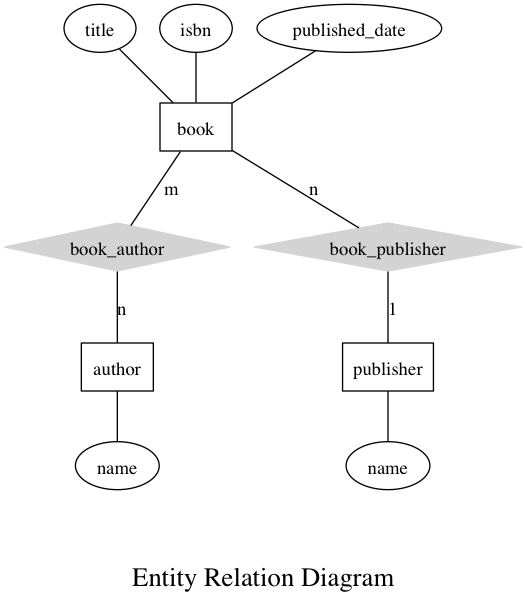
\includegraphics{code/ex18/ex8.png}

Let's translate this into a set of tables we could use in a relational database. First up are the basic entity tables for \texttt{book}, \texttt{publisher} and \texttt{author}.


\subsubsection{Book Table%
  \label{book-table}%
}

\setlength{\DUtablewidth}{\linewidth}
\begin{longtable*}[c]{|p{0.284\DUtablewidth}|p{0.458\DUtablewidth}|}
\hline
\textbf{%
Field
} & \textbf{%
Type
} \\
\hline
\endfirsthead
\hline
\textbf{%
Field
} & \textbf{%
Type
} \\
\hline
\endhead
\multicolumn{2}{c}{\hfill ... continued on next page} \\
\endfoot
\endlastfoot

Id
 & 
autoincrement int
 \\
\hline

Title
 & 
varchar (255)
 \\
\hline

ISBN
 & 
varchar (25)
 \\
\hline

Published
 & 
datetime
 \\
\hline

Publisher\_id
 & 
\texttt{Foreign Key Id} to table Publishers
 \\
\hline
\end{longtable*}

Since there is only a single \texttt{publisher} we can include a reference to the publisher entity directly in the \texttt{book} table.


\subsubsection{Publisher Table%
  \label{publisher-table}%
}

\setlength{\DUtablewidth}{\linewidth}
\begin{longtable*}[c]{|p{0.284\DUtablewidth}|p{0.412\DUtablewidth}|}
\hline
\textbf{%
Field
} & \textbf{%
Type
} \\
\hline
\endfirsthead
\hline
\textbf{%
Field
} & \textbf{%
Type
} \\
\hline
\endhead
\multicolumn{2}{c}{\hfill ... continued on next page} \\
\endfoot
\endlastfoot

Id
 & 
autoincrement int
 \\
\hline

Name
 & 
varchar (255)
 \\
\hline
\end{longtable*}


\subsubsection{Author Table%
  \label{author-table}%
}

\setlength{\DUtablewidth}{\linewidth}
\begin{longtable*}[c]{|p{0.284\DUtablewidth}|p{0.412\DUtablewidth}|}
\hline
\textbf{%
Field
} & \textbf{%
Type
} \\
\hline
\endfirsthead
\hline
\textbf{%
Field
} & \textbf{%
Type
} \\
\hline
\endhead
\multicolumn{2}{c}{\hfill ... continued on next page} \\
\endfoot
\endlastfoot

Id
 & 
autoincrement int
 \\
\hline

Name
 & 
varchar (255)
 \\
\hline
\end{longtable*}

Next up we need to define the relationships between the entities. Luckily for us the relationship between a \texttt{publisher} and a \texttt{book} is that a \texttt{publisher} can publish many \texttt{books} but a \texttt{book} can only have one \texttt{publisher}. This means we don't need a special join table to be able to retrieve both sides of the query. It's enough to just put the \texttt{publisher's id} in the \texttt{book} table.

On the other hand an \texttt{author} can have written many books and a book can have more than one \texttt{author}. We need to introduce a table to model this relation. This is called a \texttt{join table}. This table well show the relationships between individual books and authors.


\subsubsection{AuthorBook Table%
  \label{authorbook-table}%
}

\setlength{\DUtablewidth}{\linewidth}
\begin{longtable*}[c]{|p{0.284\DUtablewidth}|p{0.412\DUtablewidth}|}
\hline
\textbf{%
Field
} & \textbf{%
Type
} \\
\hline
\endfirsthead
\hline
\textbf{%
Field
} & \textbf{%
Type
} \\
\hline
\endhead
\multicolumn{2}{c}{\hfill ... continued on next page} \\
\endfoot
\endlastfoot

Book Id
 & 
\texttt{Foreign Key Id} to table Books
 \\
\hline

Author Id
 & 
\texttt{Foreign Key Id} to table Author
 \\
\hline
\end{longtable*}

Awesome we have an initial model for how to store a book. Now let's use this in our fancy OO language. Let's define a set of classes that allows us to represent a book, an author and a publisher.

\begin{Verbatim}[commandchars=\\\{\}]
\PY{c+c1}{// Helper method to make simple getter / setter}
\PY{k+kd}{var} \PY{n+nx}{simple\PYZus{}setter\PYZus{}getter} \PY{o}{=} \PY{k+kd}{function}\PY{p}{(}\PY{n+nx}{object}\PY{p}{,} \PY{n+nx}{fields}\PY{p}{,} \PY{n+nx}{name}\PY{p}{)} \PY{p}{\PYZob{}}
  \PY{n+nb}{Object}\PY{p}{.}\PY{n+nx}{defineProperty}\PY{p}{(}\PY{n+nx}{object}\PY{p}{,} \PY{n+nx}{name}\PY{p}{,} \PY{p}{\PYZob{}} \PY{n+nx}{enumerable}\PY{o}{:} \PY{k+kc}{true}
    \PY{p}{,} \PY{n+nx}{get}\PY{o}{:} \PY{k+kd}{function} \PY{p}{(}\PY{p}{)} \PY{p}{\PYZob{}} \PY{k}{return} \PY{n+nx}{fields}\PY{p}{[}\PY{n+nx}{name}\PY{p}{]}\PY{p}{;} \PY{p}{\PYZcb{}}
    \PY{p}{,} \PY{n+nx}{set}\PY{o}{:} \PY{k+kd}{function} \PY{p}{(}\PY{n+nx}{value}\PY{p}{)} \PY{p}{\PYZob{}} \PY{n+nx}{fields}\PY{p}{[}\PY{n+nx}{name}\PY{p}{]} \PY{o}{=} \PY{n+nx}{value}\PY{p}{;} \PY{p}{\PYZcb{}}
  \PY{p}{\PYZcb{}}\PY{p}{)}\PY{p}{;}
\PY{p}{\PYZcb{}}

\PY{c+c1}{// An Author entity}
\PY{k+kd}{var} \PY{n+nx}{Author} \PY{o}{=} \PY{k+kd}{function}\PY{p}{(}\PY{n+nx}{\PYZus{}name}\PY{p}{,} \PY{n+nx}{\PYZus{}books}\PY{p}{)} \PY{p}{\PYZob{}}
  \PY{k+kd}{var} \PY{n+nx}{fields} \PY{o}{=} \PY{p}{\PYZob{}}
      \PY{n+nx}{name}\PY{o}{:} \PY{n+nx}{\PYZus{}name}
    \PY{p}{,} \PY{n+nx}{books}\PY{o}{:} \PY{n+nx}{\PYZus{}books} \PY{o}{||} \PY{p}{[}\PY{p}{]}
  \PY{p}{\PYZcb{}}

  \PY{k}{this}\PY{p}{.}\PY{n+nx}{addBook} \PY{o}{=} \PY{k+kd}{function}\PY{p}{(}\PY{n+nx}{book}\PY{p}{)} \PY{p}{\PYZob{}}
    \PY{n+nx}{fields}\PY{p}{.}\PY{n+nx}{books}\PY{p}{.}\PY{n+nx}{push}\PY{p}{(}\PY{n+nx}{book}\PY{p}{)}\PY{p}{;}
  \PY{p}{\PYZcb{}}

  \PY{n+nx}{simple\PYZus{}setter\PYZus{}getter}\PY{p}{(}\PY{k}{this}\PY{p}{,} \PY{n+nx}{fields}\PY{p}{,} \PY{l+s+s2}{"name"}\PY{p}{)}\PY{p}{;}
  \PY{n+nx}{simple\PYZus{}setter\PYZus{}getter}\PY{p}{(}\PY{k}{this}\PY{p}{,} \PY{n+nx}{fields}\PY{p}{,} \PY{l+s+s2}{"books"}\PY{p}{)}\PY{p}{;}
\PY{p}{\PYZcb{}}

\PY{c+c1}{// A Published entity}
\PY{k+kd}{var} \PY{n+nx}{Publisher} \PY{o}{=} \PY{k+kd}{function}\PY{p}{(}\PY{n+nx}{\PYZus{}name}\PY{p}{,} \PY{n+nx}{\PYZus{}books}\PY{p}{)} \PY{p}{\PYZob{}}
  \PY{k+kd}{var} \PY{n+nx}{fields} \PY{o}{=} \PY{p}{\PYZob{}}
      \PY{n+nx}{name}\PY{o}{:} \PY{n+nx}{\PYZus{}name}
    \PY{p}{,} \PY{n+nx}{books}\PY{o}{:} \PY{n+nx}{\PYZus{}books} \PY{o}{||} \PY{p}{[}\PY{p}{]}
  \PY{p}{\PYZcb{}}

  \PY{k}{this}\PY{p}{.}\PY{n+nx}{addBook} \PY{o}{=} \PY{k+kd}{function}\PY{p}{(}\PY{n+nx}{book}\PY{p}{)} \PY{p}{\PYZob{}}
    \PY{n+nx}{fields}\PY{p}{.}\PY{n+nx}{books}\PY{p}{.}\PY{n+nx}{push}\PY{p}{(}\PY{n+nx}{book}\PY{p}{)}\PY{p}{;}
  \PY{p}{\PYZcb{}}

  \PY{n+nx}{simple\PYZus{}setter\PYZus{}getter}\PY{p}{(}\PY{k}{this}\PY{p}{,} \PY{n+nx}{fields}\PY{p}{,} \PY{l+s+s2}{"name"}\PY{p}{)}\PY{p}{;}
  \PY{n+nx}{simple\PYZus{}setter\PYZus{}getter}\PY{p}{(}\PY{k}{this}\PY{p}{,} \PY{n+nx}{fields}\PY{p}{,} \PY{l+s+s2}{"books"}\PY{p}{)}\PY{p}{;}
\PY{p}{\PYZcb{}}

\PY{c+c1}{// A Book entity}
\PY{k+kd}{var} \PY{n+nx}{Book} \PY{o}{=} \PY{k+kd}{function}\PY{p}{(}\PY{n+nx}{\PYZus{}isbn}\PY{p}{,} \PY{n+nx}{\PYZus{}title}\PY{p}{,} \PY{n+nx}{\PYZus{}published\PYZus{}date}\PY{p}{,} \PY{n+nx}{\PYZus{}authors}\PY{p}{,} \PY{n+nx}{\PYZus{}publisher}\PY{p}{)} \PY{p}{\PYZob{}}
  \PY{k+kd}{var} \PY{n+nx}{fields} \PY{o}{=} \PY{p}{\PYZob{}}
      \PY{n+nx}{isbn}\PY{o}{:} \PY{n+nx}{\PYZus{}isbn}
    \PY{p}{,} \PY{n+nx}{title}\PY{o}{:} \PY{n+nx}{\PYZus{}title}
    \PY{p}{,} \PY{n+nx}{published\PYZus{}date}\PY{o}{:} \PY{n+nx}{\PYZus{}published\PYZus{}date}
    \PY{p}{,} \PY{n+nx}{authors}\PY{o}{:} \PY{n+nx}{\PYZus{}authors} \PY{o}{||} \PY{p}{[}\PY{p}{]}
    \PY{p}{,} \PY{n+nx}{publisher}\PY{o}{:} \PY{n+nx}{\PYZus{}publisher}
  \PY{p}{\PYZcb{}}

  \PY{k}{this}\PY{p}{.}\PY{n+nx}{addAuthor} \PY{o}{=} \PY{k+kd}{function}\PY{p}{(}\PY{n+nx}{author}\PY{p}{)} \PY{p}{\PYZob{}}
    \PY{n+nx}{fields}\PY{p}{.}\PY{n+nx}{authors}\PY{p}{.}\PY{n+nx}{push}\PY{p}{(}\PY{n+nx}{author}\PY{p}{)}\PY{p}{;}
  \PY{p}{\PYZcb{}}

  \PY{n+nx}{simple\PYZus{}setter\PYZus{}getter}\PY{p}{(}\PY{k}{this}\PY{p}{,} \PY{n+nx}{fields}\PY{p}{,} \PY{l+s+s2}{"title"}\PY{p}{)}\PY{p}{;}
  \PY{n+nx}{simple\PYZus{}setter\PYZus{}getter}\PY{p}{(}\PY{k}{this}\PY{p}{,} \PY{n+nx}{fields}\PY{p}{,} \PY{l+s+s2}{"isbn"}\PY{p}{)}\PY{p}{;}
  \PY{n+nx}{simple\PYZus{}setter\PYZus{}getter}\PY{p}{(}\PY{k}{this}\PY{p}{,} \PY{n+nx}{fields}\PY{p}{,} \PY{l+s+s2}{"authors"}\PY{p}{)}\PY{p}{;}
  \PY{n+nx}{simple\PYZus{}setter\PYZus{}getter}\PY{p}{(}\PY{k}{this}\PY{p}{,} \PY{n+nx}{fields}\PY{p}{,} \PY{l+s+s2}{"publisher"}\PY{p}{)}\PY{p}{;}
\PY{p}{\PYZcb{}}

\PY{c+c1}{// Create a publisher}
\PY{k+kd}{var} \PY{n+nx}{publisher} \PY{o}{=} \PY{k}{new} \PY{n+nx}{Author}\PY{p}{(}\PY{l+s+s2}{"Maxwell Books"}\PY{p}{)}\PY{p}{;}
\PY{c+c1}{// Create the first author and book}
\PY{k+kd}{var} \PY{n+nx}{author1} \PY{o}{=} \PY{k}{new} \PY{n+nx}{Author}\PY{p}{(}\PY{l+s+s2}{"James"}\PY{p}{)}\PY{p}{;}
\PY{k+kd}{var} \PY{n+nx}{book1} \PY{o}{=} \PY{k}{new} \PY{n+nx}{Book}\PY{p}{(}\PY{l+s+s2}{"1"}\PY{p}{,} \PY{l+s+s2}{"Wizard"}\PY{p}{,} \PY{k}{new} \PY{n+nb}{Date}\PY{p}{(}\PY{p}{)}\PY{p}{)}\PY{p}{;}

\PY{c+c1}{// Add the author to the book}
\PY{n+nx}{book1}\PY{p}{.}\PY{n+nx}{addAuthor}\PY{p}{(}\PY{n+nx}{author1}\PY{p}{)}\PY{p}{;}
\PY{c+c1}{// Add the book to the author}
\PY{n+nx}{author1}\PY{p}{.}\PY{n+nx}{addBook}\PY{p}{(}\PY{n+nx}{book1}\PY{p}{)}\PY{p}{;}
\PY{c+c1}{// Add the publisher to the book}
\PY{n+nx}{book1}\PY{p}{.}\PY{n+nx}{publisher} \PY{o}{=} \PY{n+nx}{publisher}\PY{p}{;}
\PY{c+c1}{// Add the book to the publisher}
\PY{n+nx}{publisher}\PY{p}{.}\PY{n+nx}{addBook}\PY{p}{(}\PY{n+nx}{book1}\PY{p}{)}\PY{p}{;}

\PY{c+c1}{// Create second author and book}
\PY{k+kd}{var} \PY{n+nx}{author2} \PY{o}{=} \PY{k}{new} \PY{n+nx}{Author}\PY{p}{(}\PY{l+s+s2}{"Peter"}\PY{p}{)}\PY{p}{;}
\PY{k+kd}{var} \PY{n+nx}{book2} \PY{o}{=} \PY{k}{new} \PY{n+nx}{Book}\PY{p}{(}\PY{l+s+s2}{"2"}\PY{p}{,} \PY{l+s+s2}{"Space war"}\PY{p}{,} \PY{k}{new} \PY{n+nb}{Date}\PY{p}{(}\PY{p}{)}\PY{p}{,} \PY{p}{[}\PY{p}{]}\PY{p}{,} \PY{k+kc}{null}\PY{p}{)}\PY{p}{;}

\PY{c+c1}{// Add the author to the book}
\PY{n+nx}{book2}\PY{p}{.}\PY{n+nx}{addAuthor}\PY{p}{(}\PY{n+nx}{author2}\PY{p}{)}\PY{p}{;}
\PY{c+c1}{// Add the book to the author}
\PY{n+nx}{author2}\PY{p}{.}\PY{n+nx}{addBook}\PY{p}{(}\PY{n+nx}{book1}\PY{p}{)}\PY{p}{;}
\PY{c+c1}{// Add the publisher to the book}
\PY{n+nx}{book2}\PY{p}{.}\PY{n+nx}{publisher} \PY{o}{=} \PY{n+nx}{publisher}\PY{p}{;}
\PY{c+c1}{// Add the book to the publisher}
\PY{n+nx}{publisher}\PY{p}{.}\PY{n+nx}{addBook}\PY{p}{(}\PY{n+nx}{book2}\PY{p}{)}\PY{p}{;}
\end{Verbatim}

One thing is clear mapping one of the objects to the underlying data store requires a set of co-ordinated inserts, queries and updates as the objects are very inter-dependent. F.ex for the \texttt{author} object each \texttt{book} must be stored in the \texttt{Book} table before we can safely write to the \texttt{AuthorBook} table.

This creates a fair bit of complexity. To avoid doing this over and over Object-Relational Mappers were developed to map from a class structure to a Relational database. This layers an additional level of abstraction on top of the relational model to make OO programming more natural and to hide the decomposition that needs to occur to fit the OO model to the relational model.

There are some pain point related to this, when it comes to changing the data model as you'll likely have to change your data model in 3 places in your code (first in your code, then in your ORM and lastly in the database itself). This incurs significant cognitive cost as you'll have to keep everything straight from top to bottom. Worse situation are if your entity model no longer fits the problem you are trying to solve in code and you need to evolve the schema. This can create a fairly substantial refactoring in your code base as you need to move relationships around and thus migrate data from a schema to another.

It gets worse when trying to describe tree like structures like objects as a single object might require a multitude of join tables making the mapping less than transparent between the \texttt{class} and the storage layer below. When evolved over time the cost of change increases due to the implied complexity.

Thus one of the more important aspects of relational data modeling is to do better modeling up front to avoid the cost of mutating the schema later. It's harder to evolve the schema more naturally with the application itself.


\subsection{Document Modeling%
  \label{document-modeling}%
}

So why are document databases being em-brassed by developers. It's fairly simple. The mapping between an OO language and documents are much closer than between OO languages and relational models. Another aspect is the dynamic schema concept meaning that documents are not set in stone and can evolve without having to modify the underlying Schema definition.

Let's have a look at how we could model the Book class and it's relationships in a document database. Remember the definition of the Book class.

\begin{Verbatim}[commandchars=\\\{\}]
\PY{c+c1}{// A Book entity}
\PY{k+kd}{var} \PY{n+nx}{Book} \PY{o}{=} \PY{k+kd}{function}\PY{p}{(}\PY{n+nx}{\PYZus{}isbn}\PY{p}{,} \PY{n+nx}{\PYZus{}title}\PY{p}{,} \PY{n+nx}{\PYZus{}published\PYZus{}date}\PY{p}{,} \PY{n+nx}{\PYZus{}authors}\PY{p}{,} \PY{n+nx}{\PYZus{}publisher}\PY{p}{)} \PY{p}{\PYZob{}}
  \PY{k+kd}{var} \PY{n+nx}{fields} \PY{o}{=} \PY{p}{\PYZob{}}
      \PY{n+nx}{isbn}\PY{o}{:} \PY{n+nx}{\PYZus{}isbn}
    \PY{p}{,} \PY{n+nx}{title}\PY{o}{:} \PY{n+nx}{\PYZus{}title}
    \PY{p}{,} \PY{n+nx}{published\PYZus{}date}\PY{o}{:} \PY{n+nx}{\PYZus{}published\PYZus{}date}
    \PY{p}{,} \PY{n+nx}{authors}\PY{o}{:} \PY{n+nx}{\PYZus{}authors} \PY{o}{||} \PY{p}{[}\PY{p}{]}
    \PY{p}{,} \PY{n+nx}{publisher}\PY{o}{:} \PY{n+nx}{\PYZus{}publisher}
  \PY{p}{\PYZcb{}}

  \PY{k}{this}\PY{p}{.}\PY{n+nx}{addAuthor} \PY{o}{=} \PY{k+kd}{function}\PY{p}{(}\PY{n+nx}{author}\PY{p}{)} \PY{p}{\PYZob{}}
    \PY{n+nx}{fields}\PY{p}{.}\PY{n+nx}{authors}\PY{p}{.}\PY{n+nx}{push}\PY{p}{(}\PY{n+nx}{author}\PY{p}{)}\PY{p}{;}
  \PY{p}{\PYZcb{}}

  \PY{n+nx}{simple\PYZus{}setter\PYZus{}getter}\PY{p}{(}\PY{k}{this}\PY{p}{,} \PY{n+nx}{fields}\PY{p}{,} \PY{l+s+s2}{"title"}\PY{p}{)}\PY{p}{;}
  \PY{n+nx}{simple\PYZus{}setter\PYZus{}getter}\PY{p}{(}\PY{k}{this}\PY{p}{,} \PY{n+nx}{fields}\PY{p}{,} \PY{l+s+s2}{"isbn"}\PY{p}{)}\PY{p}{;}
  \PY{n+nx}{simple\PYZus{}setter\PYZus{}getter}\PY{p}{(}\PY{k}{this}\PY{p}{,} \PY{n+nx}{fields}\PY{p}{,} \PY{l+s+s2}{"authors"}\PY{p}{)}\PY{p}{;}
  \PY{n+nx}{simple\PYZus{}setter\PYZus{}getter}\PY{p}{(}\PY{k}{this}\PY{p}{,} \PY{n+nx}{fields}\PY{p}{,} \PY{l+s+s2}{"publisher"}\PY{p}{)}\PY{p}{;}
\PY{p}{\PYZcb{}}
\end{Verbatim}

How could this look as a document? Well let's create a JSON (JavaScript Object Notation) document to show a possible schema design. The first document represents a book, the second one an author and the third one a publisher.


\subsubsection{Book%
  \label{book}%
}

\begin{Verbatim}[commandchars=\\\{\}]
\PY{p}{\PYZob{}}
    \PY{n+nt}{"id"}\PY{p}{:} \PY{l+m+mi}{1}
  \PY{p}{,} \PY{n+nt}{"title"}\PY{p}{:} \PY{l+s+s2}{"Moby Dick"}
  \PY{p}{,} \PY{n+nt}{"isbn"}\PY{p}{:} \PY{l+s+s2}{"978-1853260087"}
  \PY{p}{,} \PY{n+nt}{"published"}\PY{p}{:} \PY{l+m+mi}{1992}
  \PY{p}{,} \PY{n+nt}{"authors"}\PY{p}{:} \PY{p}{[}\PY{p}{\PYZob{}}
        \PY{n+nt}{"id"}\PY{p}{:} \PY{l+m+mi}{1}
      \PY{p}{,} \PY{n+nt}{"name"}\PY{p}{:} \PY{l+s+s2}{"Herman Melville"}
    \PY{p}{\PYZcb{}}\PY{p}{]}
  \PY{p}{,} \PY{n+nt}{"publisher"}\PY{p}{:} \PY{p}{\PYZob{}}
      \PY{n+nt}{"id"}\PY{p}{:} \PY{l+m+mi}{1}
    \PY{p}{,} \PY{n+nt}{"name"}\PY{p}{:} \PY{l+s+s2}{"Wordsworth Editions Ltd"}
  \PY{p}{\PYZcb{}}
\PY{p}{\PYZcb{}}
\end{Verbatim}


\subsubsection{Author%
  \label{author}%
}

\begin{Verbatim}[commandchars=\\\{\}]
\PY{p}{\PYZob{}}
    \PY{n+nt}{"id"}\PY{p}{:} \PY{l+m+mi}{1}
  \PY{p}{,} \PY{n+nt}{"name"}\PY{p}{:} \PY{l+s+s2}{"Herman Melville"}
  \PY{p}{,} \PY{n+nt}{"books"}\PY{p}{:} \PY{p}{[}\PY{l+m+mi}{1}\PY{p}{]}
\PY{p}{\PYZcb{}}
\end{Verbatim}


\subsubsection{Publisher%
  \label{publisher}%
}

\begin{Verbatim}[commandchars=\\\{\}]
\PY{p}{\PYZob{}}
    \PY{n+nt}{"id"}\PY{p}{:} \PY{l+m+mi}{1}
  \PY{p}{,} \PY{n+nt}{"name"}\PY{p}{:} \PY{l+s+s2}{"Wordsworth Editions Ltd"}
  \PY{p}{,} \PY{n+nt}{"books"}\PY{p}{:} \PY{p}{[}\PY{l+m+mi}{1}\PY{p}{]}
  \PY{p}{,} \PY{n+nt}{"authors"}\PY{p}{:} \PY{p}{[}\PY{l+m+mi}{1}\PY{p}{]}
\PY{p}{\PYZcb{}}
\end{Verbatim}

Notice somethings? The data and context of the data is bundled together in the document making a document self descriptive. Also we have nested documents in the \texttt{Book} document for the \texttt{authors} and the \texttt{publisher}. This matches very closely to how the actual \texttt{Book} classes internal \texttt{fields} are laid out. The level off abstraction between the model and the data in the database is lower.

This is especially evident if we decide to introduce a new concept like a review. Let's add the review concept to the \texttt{Book} class.

\begin{Verbatim}[commandchars=\\\{\}]
\PY{c+c1}{// A Book entity}
\PY{k+kd}{var} \PY{n+nx}{Book} \PY{o}{=} \PY{k+kd}{function}\PY{p}{(}\PY{n+nx}{\PYZus{}isbn}\PY{p}{,} \PY{n+nx}{\PYZus{}title}\PY{p}{,} \PY{n+nx}{\PYZus{}published\PYZus{}date}\PY{p}{,} \PY{n+nx}{\PYZus{}authors}\PY{p}{,} \PY{n+nx}{\PYZus{}publisher}\PY{p}{,} \PY{n+nx}{\PYZus{}reviews}\PY{p}{)} \PY{p}{\PYZob{}}
  \PY{k+kd}{var} \PY{n+nx}{fields} \PY{o}{=} \PY{p}{\PYZob{}}
      \PY{n+nx}{isbn}\PY{o}{:} \PY{n+nx}{\PYZus{}isbn}
    \PY{p}{,} \PY{n+nx}{title}\PY{o}{:} \PY{n+nx}{\PYZus{}title}
    \PY{p}{,} \PY{n+nx}{published\PYZus{}date}\PY{o}{:} \PY{n+nx}{\PYZus{}published\PYZus{}date}
    \PY{p}{,} \PY{n+nx}{authors}\PY{o}{:} \PY{n+nx}{\PYZus{}authors} \PY{o}{||} \PY{p}{[}\PY{p}{]}
    \PY{p}{,} \PY{n+nx}{publisher}\PY{o}{:} \PY{n+nx}{\PYZus{}publisher}
    \PY{p}{,} \PY{n+nx}{reviews}\PY{o}{:} \PY{n+nx}{\PYZus{}reviews}
  \PY{p}{\PYZcb{}}

  \PY{k}{this}\PY{p}{.}\PY{n+nx}{addAuthor} \PY{o}{=} \PY{k+kd}{function}\PY{p}{(}\PY{n+nx}{author}\PY{p}{)} \PY{p}{\PYZob{}}
    \PY{n+nx}{fields}\PY{p}{.}\PY{n+nx}{authors}\PY{p}{.}\PY{n+nx}{push}\PY{p}{(}\PY{n+nx}{author}\PY{p}{)}\PY{p}{;}
  \PY{p}{\PYZcb{}}

  \PY{k}{this}\PY{p}{.}\PY{n+nx}{addReview} \PY{o}{=} \PY{k+kd}{function}\PY{p}{(}\PY{n+nx}{review}\PY{p}{)} \PY{p}{\PYZob{}}
    \PY{n+nx}{fields}\PY{p}{.}\PY{n+nx}{reviews}\PY{p}{.}\PY{n+nx}{push}\PY{p}{(}\PY{n+nx}{review}\PY{p}{)}\PY{p}{;}
  \PY{p}{\PYZcb{}}

  \PY{n+nx}{simple\PYZus{}setter\PYZus{}getter}\PY{p}{(}\PY{k}{this}\PY{p}{,} \PY{n+nx}{fields}\PY{p}{,} \PY{l+s+s2}{"title"}\PY{p}{)}\PY{p}{;}
  \PY{n+nx}{simple\PYZus{}setter\PYZus{}getter}\PY{p}{(}\PY{k}{this}\PY{p}{,} \PY{n+nx}{fields}\PY{p}{,} \PY{l+s+s2}{"isbn"}\PY{p}{)}\PY{p}{;}
  \PY{n+nx}{simple\PYZus{}setter\PYZus{}getter}\PY{p}{(}\PY{k}{this}\PY{p}{,} \PY{n+nx}{fields}\PY{p}{,} \PY{l+s+s2}{"authors"}\PY{p}{)}\PY{p}{;}
  \PY{n+nx}{simple\PYZus{}setter\PYZus{}getter}\PY{p}{(}\PY{k}{this}\PY{p}{,} \PY{n+nx}{fields}\PY{p}{,} \PY{l+s+s2}{"publisher"}\PY{p}{)}\PY{p}{;}
  \PY{n+nx}{simple\PYZus{}setter\PYZus{}getter}\PY{p}{(}\PY{k}{this}\PY{p}{,} \PY{n+nx}{fields}\PY{p}{,} \PY{l+s+s2}{"reviews"}\PY{p}{)}\PY{p}{;}
\PY{p}{\PYZcb{}}
\end{Verbatim}

Now let's see how that could be reflected in a the document for the \texttt{Book}.

\begin{Verbatim}[commandchars=\\\{\}]
\PY{p}{\PYZob{}}
    \PY{n+nt}{"id"}\PY{p}{:} \PY{l+m+mi}{1}
  \PY{p}{,} \PY{n+nt}{"title"}\PY{p}{:} \PY{l+s+s2}{"Moby Dick"}
  \PY{p}{,} \PY{n+nt}{"isbn"}\PY{p}{:} \PY{l+s+s2}{" 978-1853260087"}
  \PY{p}{,} \PY{n+nt}{"published"}\PY{p}{:} \PY{l+m+mi}{1992}
  \PY{p}{,} \PY{n+nt}{"authors"}\PY{p}{:} \PY{p}{[}\PY{p}{\PYZob{}}
        \PY{n+nt}{"id"}\PY{p}{:} \PY{l+m+mi}{1}
      \PY{p}{,} \PY{n+nt}{"name"}\PY{p}{:} \PY{l+s+s2}{"Herman Melville"}
    \PY{p}{\PYZcb{}}\PY{p}{]}
  \PY{p}{,} \PY{n+nt}{"publisher"}\PY{p}{:} \PY{p}{\PYZob{}}
      \PY{n+nt}{"id"}\PY{p}{:} \PY{l+m+mi}{1}
    \PY{p}{,} \PY{n+nt}{"name"}\PY{p}{:} \PY{l+s+s2}{"Wordsworth Editions Ltd"}
  \PY{p}{\PYZcb{}}
  \PY{p}{,} \PY{n+nt}{"reviews"}\PY{p}{:} \PY{p}{[}\PY{p}{\PYZob{}}
      \PY{n+nt}{"id"}\PY{p}{:} \PY{l+m+mi}{1}
    \PY{p}{,} \PY{n+nt}{"review"}\PY{p}{:} \PY{l+s+s2}{"Awesome book, loved the whale"}
    \PY{p}{,} \PY{n+nt}{"stars"}\PY{p}{:} \PY{l+m+mi}{5}
  \PY{p}{\PYZcb{}}\PY{p}{]}
\PY{p}{\PYZcb{}}
\end{Verbatim}

As you can see the mapping between the OO class and the data stored in the database is close to 1:1. In a relational database this would require an additional \texttt{Review} table and a \texttt{BookReviews} join table requiring additional logic to map back and forth between the OO class and the data model.


\subsection{Things To Note%
  \label{things-to-note}%
}

Our world is made up of data object that change structure over time. Document databases have become more and more popular as they embrace the concept of evolving data structures better than traditional relational databases and map better to the way computer programming languages model data. In later exercises we will go ahead and build our very own simple ODM (object document mapping) library to help us make the mapping more simple and get a feel on how to map data back and forth. We will also briefly introduce the Mongoose ODM as more full featured version of our simple attempt at abstraction. But first things first. We are going to explore different schema designs and the pros and cons of each.


\section{Exercise 19: Evolving A Simple Schema%
  \label{exercise-19-evolving-a-simple-schema}%
}

Let's put together some of the stuff we have covered including inserts, updates with atomic updates and removes to create a little book lending library application. We are going to focus on only the actual code around the book library itself in this chapter and then in the next chapter provide a very simple rest \texttt{API} to out library application so we can integrate it into the next \texttt{facebook} of library lending called \texttt{bookface}.

Let's fact model our library model concepts.


\subsection{Facts%
  \label{id2}%
}


\subsubsection{Book%
  \label{id3}%
}
%
\begin{itemize}

\item A Book has the title \texttt{Fall of the Roman Empire}

\item The Book \texttt{Fall of the Roman Empire} has the unique id 1

\item The Book \texttt{Fall of the Roman Empire} has a 1973 Edition

\item The Book \texttt{Fall of the Roman Empire} was published by \texttt{T Books} in 1973

\item The Book \texttt{Fall of the Roman Empire} is identified by the ISBN number \texttt{978-1853260087}

\item The Book \texttt{Fall of the Roman Empire} was written by the Author \texttt{James W Kirk}

\item The Book \texttt{Fall of the Roman Empire} has the summary \texttt{The road to the fall of the Roman Empire}, a comprehensive history of the greatest western empire's decline``

\item The 1973 Edition of \texttt{Fall of the Roman Empire} was loaned by the User \texttt{Peter Griffin} on the 19th of June 1976.

\item The 1973 Edition of \texttt{Fall of the Roman Empire} that was loaned by the User \texttt{Peter Griffin} on the 1th of June 1986 should be returned on the 15th of June 1986.

\end{itemize}


\subsubsection{Edition%
  \label{edition}%
}
%
\begin{itemize}

\item The Edition of \texttt{Fall of the Roman Empire} is Published by \texttt{T Books}

\item The Edition of \texttt{Fall of the Roman Empire} was Published in 1973

\item The Library has 4 copies of the 1973 Edition of the \texttt{Fall of the Roman Empire}

\end{itemize}


\subsubsection{Author%
  \label{id4}%
}
%
\begin{itemize}

\item The Author \texttt{James W Kirk} wrote the book \texttt{Fall of the Roman Empire}

\item The Author \texttt{James W Kirk} wrote the book ''The Rise of the Roman Empire``

\end{itemize}


\subsubsection{Publisher%
  \label{id5}%
}
%
\begin{itemize}

\item The Publisher \texttt{T Books} published the 1973 Edition of the Book \texttt{Fall of the Roman Empire}

\item The Publisher \texttt{T Books} has published the 1967 Edition of the Book \texttt{Wizard of Oz}

\item The Publisher is names \texttt{T Books}

\end{itemize}


\subsubsection{User%
  \label{user}%
}
%
\begin{itemize}

\item The User \texttt{Peter Griffin} loaned the Book \texttt{Fall of the Roman Empire} on the 1st of June 1986.

\item The User \texttt{Peter Griffin} has to return the Book \texttt{Fall of the Roman Empire} on the 15th of June 1986.

\item A User is named \texttt{Peter Griffin}

\end{itemize}

Awesome we have a lot of facts to model around. Let's try to organize them in documents.


\subsection{Document Representation%
  \label{document-representation}%
}

We've identified 4 different entities that we can potentially model as documents. Let's start by roughly sketch them out.

Let's consider the \texttt{User} entity described above. We know the user has a \texttt{name} and can \texttt{loan} books for a defined period of time. Let's model the data and see how we can interact with the model.


\subsubsection{User Document%
  \label{user-document}%
}
%
\begin{quote}{\ttfamily \raggedright \noindent
\DUrole{p}{\{}~\\
~~~~\DUrole{s2}{"\_id"}\DUrole{o}{:}~\DUrole{mi}{1}~\\
~~\DUrole{p}{,}~\DUrole{s2}{"name"}\DUrole{o}{:}~\DUrole{s2}{"Peter~Griffin"}~\\
~~\DUrole{p}{,}~\DUrole{s2}{"loaned\_books"}\DUrole{o}{:}~\DUrole{p}{{[}}~\\
~~~~~~\DUrole{p}{\{}~\\
~~~~~~~~~~\DUrole{s2}{"id"}\DUrole{o}{:}~\DUrole{mi}{1}~\\
~~~~~~~~\DUrole{p}{,}~\DUrole{s2}{"title"}\DUrole{o}{:}~\DUrole{s2}{"Fall~of~the~Roman~Empire"}~\\
~~~~~~~~\DUrole{p}{,}~\DUrole{s2}{"loaned\_on"}\DUrole{o}{:}~\DUrole{s2}{"1st~of~June~1986"}~\\
~~~~~~~~\DUrole{p}{,}~\DUrole{s2}{"due\_on"}\DUrole{o}{:}~\DUrole{s2}{"15th~of~June~1986"}~\\
~~~~~~\DUrole{p}{\}}~\\
~~~~\DUrole{p}{{]}}~\\
\DUrole{p}{\}}
}
\end{quote}

We added an embedded array of documents called \texttt{loaned\_books} that contain documents representing each loaned book ''Peter Griffin`` has checked out of the library. In this case it's the 1973 edition of the ''Fall of the Roman Empire`` \texttt{Book}. What kind of operations would be performed on this document. For the \texttt{User} have decided to embed \texttt{loaned} books as an embedded array for each of retrieval and since the amount of books on loan is not likely to be very big for a given \texttt{User}.
\setcounter{listcnt0}{0}
\begin{list}{\arabic{listcnt0}.}
{
\usecounter{listcnt0}
\setlength{\rightmargin}{\leftmargin}
}

\item Add a new loan to the user document
\end{list}
%
\begin{quote}{\ttfamily \raggedright \noindent
\DUrole{nx}{db}\DUrole{p}{.}\DUrole{nx}{collection}\DUrole{p}{(}\DUrole{s1}{'users'}\DUrole{p}{).}\DUrole{nx}{update}\DUrole{p}{(}~\\
~~~~\DUrole{p}{\{}\DUrole{nx}{\_id}\DUrole{o}{:}~\DUrole{mi}{1}\DUrole{p}{\}}~\\
~~\DUrole{p}{,}~\DUrole{p}{\{}~\\
~~~~~~\DUrole{nx}{\$push}\DUrole{o}{:}~\DUrole{p}{\{}\DUrole{nx}{loaned\_books}\DUrole{o}{:}~\DUrole{p}{\{}~\\
~~~~~~~~~~\DUrole{nx}{id}\DUrole{o}{:}~\DUrole{mi}{2}~\\
~~~~~~~~\DUrole{p}{,}~\DUrole{nx}{title}\DUrole{o}{:}~\DUrole{s2}{"Wizard~of~Oz"}~\\
~~~~~~~~\DUrole{p}{,}~\DUrole{nx}{loaned\_on}\DUrole{o}{:}~\DUrole{nx}{start\_date}~\\
~~~~~~~~\DUrole{p}{,}~\DUrole{nx}{due\_on}\DUrole{o}{:}~\DUrole{nx}{due\_date}~\\
~~~~~~\DUrole{p}{\}\}}~\\
~~~~\DUrole{p}{\},}~\DUrole{kd}{function}\DUrole{p}{(}\DUrole{nx}{err}\DUrole{p}{,}~\DUrole{nx}{result}\DUrole{p}{)}~\DUrole{p}{\{}\DUrole{p}{\})}
}
\end{quote}
\setcounter{listcnt0}{0}
\begin{list}{\arabic{listcnt0}.}
{
\usecounter{listcnt0}
\addtocounter{listcnt0}{1}
\setlength{\rightmargin}{\leftmargin}
}

\item Remove a book from the user and return it to the library
\end{list}
%
\begin{quote}{\ttfamily \raggedright \noindent
\DUrole{nx}{db}\DUrole{p}{.}\DUrole{nx}{collection}\DUrole{p}{(}\DUrole{s1}{'users'}\DUrole{p}{).}\DUrole{nx}{update}\DUrole{p}{(}~\\
~~~~\DUrole{p}{\{}\DUrole{nx}{\_id}\DUrole{o}{:}~\DUrole{mi}{1}\DUrole{p}{\}}~\\
~~\DUrole{p}{,}~\DUrole{p}{\{}~\\
~~~~~~\DUrole{nx}{\$pop}\DUrole{o}{:}~\DUrole{p}{\{}\DUrole{nx}{loaned\_books}\DUrole{o}{:}~\DUrole{p}{\{}\DUrole{nx}{id}\DUrole{o}{:}\DUrole{mi}{2}\DUrole{p}{\}\}}~\\
~~~~\DUrole{p}{\},}~\DUrole{kd}{function}\DUrole{p}{(}\DUrole{nx}{err}\DUrole{p}{,}~\DUrole{nx}{result}\DUrole{p}{)}~\DUrole{p}{\{}\DUrole{p}{\})}
}
\end{quote}
\setcounter{listcnt0}{0}
\begin{list}{\arabic{listcnt0}.}
{
\usecounter{listcnt0}
\addtocounter{listcnt0}{2}
\setlength{\rightmargin}{\leftmargin}
}

\item Extend a loan period (change the due date)
\end{list}
%
\begin{quote}{\ttfamily \raggedright \noindent
\DUrole{nx}{db}\DUrole{p}{.}\DUrole{nx}{collection}\DUrole{p}{(}\DUrole{s1}{'users'}\DUrole{p}{).}\DUrole{nx}{update}\DUrole{p}{(}~\\
~~~~\DUrole{p}{\{}\DUrole{nx}{\_id}\DUrole{o}{:}~\DUrole{mi}{1}\DUrole{p}{,}~\DUrole{s2}{"loaned\_on.id"}\DUrole{o}{:}~\DUrole{mi}{2}\DUrole{p}{\}}~\\
~~\DUrole{p}{,}~\DUrole{p}{\{}~\\
~~~~~~\DUrole{nx}{\$set}\DUrole{o}{:}~\DUrole{p}{\{}~\\
~~~~~~~~\DUrole{s2}{"loaned\_on.\$.due\_on"}\DUrole{o}{:}~\DUrole{nx}{new\_due\_date}~\\
~~~~~~\DUrole{p}{\}}~\\
~~~~\DUrole{p}{\},}~\DUrole{kd}{function}\DUrole{p}{(}\DUrole{nx}{err}\DUrole{p}{,}~\DUrole{nx}{result}\DUrole{p}{)}~\DUrole{p}{\{}\DUrole{p}{\})}
}
\end{quote}

Let's look at a possible Author document.


\subsubsection{Author Document%
  \label{author-document}%
}
%
\begin{quote}{\ttfamily \raggedright \noindent
\DUrole{p}{\{}~\\
~~~~\DUrole{s2}{"\_id"}\DUrole{o}{:}~\DUrole{mi}{1}~\\
~~\DUrole{p}{,}~\DUrole{s2}{"name"}\DUrole{o}{:}~\DUrole{s2}{"James~W~Kirk"}~\\
\DUrole{p}{\}}
}
\end{quote}

As you can see we don't include an array of authored \texttt{Book} id's because we will be including the array of authors in the \texttt{Book} document so we can easily browse books by author. This is similar to the traditional \texttt{1:N} relational database relationship.

Similarly a publisher is represented as a separate document.


\subsubsection{Publisher Document%
  \label{publisher-document}%
}
%
\begin{quote}{\ttfamily \raggedright \noindent
\DUrole{p}{\{}~\\
~~~~\DUrole{s2}{"\_id"}\DUrole{o}{:}~\DUrole{mi}{1}~\\
~~\DUrole{p}{,}~\DUrole{s2}{"name"}\DUrole{o}{:}~\DUrole{s2}{"T~Books"}~\\
\DUrole{p}{\}}
}
\end{quote}

As you can see we don't include an array of published \texttt{Book} id's because we will be including the \texttt{publisher\_id} in the \texttt{Book} document so we can easily browse books by publisher. This is similar to the traditional \texttt{1:N} relational database relationship.

Let's Have a look at the central concept in our library, namely the \texttt{Book}. Let's take a look at the document.


\subsubsection{Book Document%
  \label{book-document}%
}
%
\begin{quote}{\ttfamily \raggedright \noindent
\DUrole{p}{\{}~\\
~~\DUrole{c1}{//~Individual~Edition~id\\
}~~~~\DUrole{s2}{"\_id"}\DUrole{o}{:}~\DUrole{mi}{1}~\\
~~\DUrole{p}{,}~\DUrole{s2}{"title"}\DUrole{o}{:}~\DUrole{s2}{"Fall~of~the~Roman~Empire"}~\\
~\\
~~\DUrole{c1}{//~Shared~id~for~all~"Fall~of~the~Roman~Empire"~books\\
}~~\DUrole{p}{,}~\DUrole{s2}{"origin\_id"}\DUrole{o}{:}~\DUrole{mi}{1}~\\
~\\
~~\DUrole{c1}{//~Information~about~the~publisher\\
}~~\DUrole{p}{,}~\DUrole{s2}{"publisher"}\DUrole{o}{:}~\DUrole{p}{\{}~\\
~~~~~~\DUrole{s2}{"published"}\DUrole{o}{:}~\DUrole{mi}{1973}~\\
~~~~\DUrole{p}{,}~\DUrole{s2}{"edition"}\DUrole{o}{:}~\DUrole{mi}{4}~\\
~~~~\DUrole{p}{,}~\DUrole{s2}{"publisher\_id"}\DUrole{o}{:}~\DUrole{mi}{1}~\\
~~~~\DUrole{p}{,}~\DUrole{s2}{"publisher"}\DUrole{o}{:}~\DUrole{s2}{"T~Books"}~\\
~~\DUrole{p}{\}}~\\
~\\
~~\DUrole{c1}{//~Book~Authors\\
}~~\DUrole{p}{,}~\DUrole{s2}{"authors"}\DUrole{o}{:}~\DUrole{p}{{[}}~\\
~~~~~~\DUrole{p}{\{}~\\
~~~~~~~~~~\DUrole{s2}{"id"}\DUrole{o}{:}~\DUrole{mi}{1}~\\
~~~~~~~~\DUrole{p}{,}~\DUrole{s2}{"name"}\DUrole{o}{:}~\DUrole{s2}{"James~W~Kirk"}~\\
~~~~~~\DUrole{p}{\}}~\\
~~~~\DUrole{p}{{]}}~\\
~\\
~~\DUrole{c1}{//~State~of~book\\
}~~\DUrole{p}{,}~\DUrole{nx}{loaned\_out}\DUrole{o}{:}~\DUrole{kc}{true}~\\
~\\
~~\DUrole{c1}{//~Books~lent~out\\
}~~\DUrole{p}{,}~\DUrole{s2}{"loaned\_out\_to"}\DUrole{o}{:}~\DUrole{p}{\{}~\\
~~~~~~~~\DUrole{s2}{"user\_id"}\DUrole{o}{:}~\DUrole{mi}{1}~\\
~~~~~~\DUrole{p}{,}~\DUrole{s2}{"loaned\_on"}\DUrole{o}{:}~\DUrole{s2}{"1st~of~June~1986"}~\\
~~~~~~\DUrole{p}{,}~\DUrole{s2}{"due\_on"}\DUrole{o}{:}~\DUrole{s2}{"15th~of~June~1986"}~\\
~~~~\DUrole{p}{\}}~\\
\DUrole{p}{\}}
}
\end{quote}

As you can see the schema for the \texttt{Book} is quite a bit more complex than the other concepts in the database. Let's look at the some of the values and what they mean.

\setlength{\DUtablewidth}{\linewidth}
\begin{longtable*}[c]{|p{0.235\DUtablewidth}|p{0.705\DUtablewidth}|}
\hline
\textbf{%
Field
} & \textbf{%
Description
} \\
\hline
\endfirsthead
\hline
\textbf{%
Field
} & \textbf{%
Description
} \\
\hline
\endhead
\multicolumn{2}{c}{\hfill ... continued on next page} \\
\endfoot
\endlastfoot

origin\_id
 & 
This id is shared by all editions of a specific book
 \\
\hline

publisher
 & 
Embedded document with all the publisher information for easy access
 \\
\hline

authors
 & 
An array of embedded author documents
 \\
\hline

loaned\_out
 & 
Embedded document containing information about the user who has borrowed the book
 \\
\hline
\end{longtable*}

So what kind of operation could we do on this document.
\setcounter{listcnt0}{0}
\begin{list}{\arabic{listcnt0}.}
{
\usecounter{listcnt0}
\setlength{\rightmargin}{\leftmargin}
}

\item Locate a \texttt{Fall of the Roman Empire} book that is not currently loaned out
\end{list}
%
\begin{quote}{\ttfamily \raggedright \noindent
\DUrole{nx}{db}\DUrole{p}{.}\DUrole{nx}{collection}\DUrole{p}{(}\DUrole{s1}{'books'}\DUrole{p}{).}\DUrole{nx}{findOne}\DUrole{p}{(}\DUrole{p}{\{}~\\
~~~~\DUrole{nx}{title}\DUrole{o}{:}~\DUrole{sr}{/\textasciicircum{}Fall~of~the~Roman/}~\\
~~\DUrole{p}{,}~\DUrole{nx}{loaned\_out}\DUrole{o}{:}\DUrole{kc}{false}~\\
\DUrole{p}{\},}~\DUrole{kd}{function}\DUrole{p}{(}\DUrole{nx}{err}\DUrole{p}{,}~\DUrole{nx}{doc}\DUrole{p}{)}~\DUrole{p}{\{}\DUrole{p}{\});}
}
\end{quote}
\setcounter{listcnt0}{0}
\begin{list}{\arabic{listcnt0}.}
{
\usecounter{listcnt0}
\addtocounter{listcnt0}{1}
\setlength{\rightmargin}{\leftmargin}
}

\item Locate all the books for %
\raisebox{1em}{\hypertarget{id7}{}}\hyperlink{id6}{\textbf{\color{red}``}}Fall of the Roman Empire currently out for loan.

\DUadmonition[system-message]{
\DUtitle[system-message]{system-message}
\raisebox{1em}{\hypertarget{id6}{}}

{\color{red}WARNING/2} in \texttt{learn-x-the-hard-way.rst}, line~5739

\hyperlink{id7}{
Inline literal start-string without end-string.
}}
\end{list}
%
\begin{quote}{\ttfamily \raggedright \noindent
\DUrole{nx}{db}\DUrole{p}{.}\DUrole{nx}{collection}\DUrole{p}{(}\DUrole{s1}{'books'}\DUrole{p}{).}\DUrole{nx}{findOne}\DUrole{p}{(}\DUrole{p}{\{}~\\
~~~~\DUrole{nx}{title}\DUrole{o}{:}~\DUrole{sr}{/\textasciicircum{}Fall~of~the~Roman/}~\\
~~\DUrole{p}{,}~\DUrole{nx}{loaned\_out}\DUrole{o}{:}\DUrole{kc}{false}~\\
\DUrole{p}{\},}~\DUrole{kd}{function}\DUrole{p}{(}\DUrole{nx}{err}\DUrole{p}{,}~\DUrole{nx}{doc}\DUrole{p}{)}~\DUrole{p}{\{}\DUrole{p}{\});}
}
\end{quote}
\setcounter{listcnt0}{0}
\begin{list}{\arabic{listcnt0}.}
{
\usecounter{listcnt0}
\addtocounter{listcnt0}{2}
\setlength{\rightmargin}{\leftmargin}
}

\item Loan one of the \texttt{Fall of the Roman Empire} books out
\end{list}
%
\begin{quote}{\ttfamily \raggedright \noindent
\DUrole{nx}{db}\DUrole{p}{.}\DUrole{nx}{collection}\DUrole{p}{(}\DUrole{s1}{'books'}\DUrole{p}{).}\DUrole{nx}{update}\DUrole{p}{(}\DUrole{p}{\{}~\\
~~\DUrole{nx}{\_id}\DUrole{o}{:}~\DUrole{mi}{1}\DUrole{p}{,}~\DUrole{nx}{loaned\_out\_to}\DUrole{o}{:}~\DUrole{p}{\{}\DUrole{nx}{\$exists}\DUrole{o}{:}~\DUrole{kc}{false}\DUrole{p}{\}}~\\
\DUrole{p}{\},}~\DUrole{p}{\{}~\\
~~~~\DUrole{nx}{\$set}\DUrole{o}{:}~\DUrole{p}{\{}~\\
~~~~~~\DUrole{nx}{loaned\_out}\DUrole{o}{:}~\DUrole{kc}{true}~\\
~~~~\DUrole{p}{,}~\DUrole{nx}{loaned\_out\_to}\DUrole{o}{:}~\DUrole{p}{\{}~\\
~~~~~~~~~~\DUrole{nx}{user\_id}\DUrole{o}{:}~\DUrole{mi}{1}~\\
~~~~~~~~\DUrole{p}{,}~\DUrole{nx}{loaned\_on}\DUrole{o}{:}~\DUrole{k}{new}~\DUrole{nb}{Date}\DUrole{p}{(}\DUrole{p}{)}~\\
~~~~~~~~\DUrole{p}{,}~\DUrole{nx}{due\_on}\DUrole{o}{:}~\DUrole{nx}{due\_date\_variable}~\\
~~~~~~\DUrole{p}{\}}~\\
~~~~\DUrole{p}{\}}~\\
\DUrole{p}{\},}~\DUrole{kd}{function}\DUrole{p}{(}\DUrole{nx}{err}\DUrole{p}{,}~\DUrole{nx}{doc}\DUrole{p}{)}~\DUrole{p}{\{}\DUrole{p}{\});}
}
\end{quote}

The first thing to notice is that the \texttt{update selector} contains not only the \texttt{\_id} of the \texttt{Book} we are loaning out but also a requirement that the field \texttt{loaned\_out} should be false. This way we ensure the update fails if someone else checked out the book before our update got run. If we do correctly find the valid document where \texttt{loaned\_out} is still \texttt{false} we set the the \texttt{loaned\_out} field to true and update the \texttt{loaned\_out\_to} field to the user who is borrowing the book.
\setcounter{listcnt0}{0}
\begin{list}{\arabic{listcnt0}.}
{
\usecounter{listcnt0}
\addtocounter{listcnt0}{3}
\setlength{\rightmargin}{\leftmargin}
}

\item Return the \texttt{Fall of the Roman Empire} book to the library
\end{list}
%
\begin{quote}{\ttfamily \raggedright \noindent
\DUrole{nx}{db}\DUrole{p}{.}\DUrole{nx}{collection}\DUrole{p}{(}\DUrole{s1}{'books'}\DUrole{p}{).}\DUrole{nx}{update}\DUrole{p}{(}\DUrole{p}{\{}~\\
~~~~\DUrole{nx}{\_id}\DUrole{o}{:}~\DUrole{mi}{1}~\\
~~\DUrole{p}{,}~\DUrole{s2}{"loaned\_out\_to.user\_id"}\DUrole{o}{:}~\DUrole{mi}{1}~\\
\DUrole{p}{\},}~\DUrole{p}{\{}~\\
~~\DUrole{nx}{\$set}\DUrole{o}{:}~\DUrole{p}{\{}~\\
~~~~~~\DUrole{nx}{loaned\_out}\DUrole{o}{:}~\DUrole{kc}{false}~\\
~~~~\DUrole{p}{,}~\DUrole{nx}{loaned\_out\_to}\DUrole{o}{:}~\DUrole{kc}{null}~\\
~~\DUrole{p}{\}}~\\
\DUrole{p}{\},}~\DUrole{kd}{function}\DUrole{p}{(}\DUrole{nx}{err}\DUrole{p}{,}~\DUrole{nx}{doc}\DUrole{p}{)}~\DUrole{p}{\{}\DUrole{p}{\});}
}
\end{quote}

This concludes the schema design for our simple library application. In the next chapter we will implement a \texttt{REST} api that allows you to write your frontend code for the library application.


\section{Exercise 20: A RESTFul Programming exercise%
  \label{exercise-20-a-restful-programming-exercise}%
}

Let's get cracking on the RESTful experience for our application. We are of course going to do this simply and from scratch so we won't be using such fancy things as express but instead keep it real with low level code (makes it easier to keep this exercise up to data aswell as we won't be tied to changes in Express.JS so much).

We are of course ignoring any sort of concept of user security sessions and such trivial real world important features.

\DUadmonition[note]{
\DUtitle[note]{Note}

What's a \texttt{REST API} you might ask. \texttt{HTTP} contains several verbs that make up what we call \texttt{CRUD} operations. These verbs are \texttt{GET}, \texttt{POST}, \texttt{PUT} and \texttt{DELETE}. Think off them as basic verbs of modifying a document. So \texttt{GET} would be equivalent to a \texttt{MongoDB find} operation, \texttt{POST} would be an \texttt{insert}, \texttt{PUT} an \texttt{update} and \texttt{DELETE} a remove. Bare with us as we will cover them in more detail as we implement our \texttt{API}.
}


\subsection{It's alive%
  \label{it-s-alive}%
}

Let's get the code up and running and let's print the most useless but also the most common greeting in all programming tutorial. I present the ''Hello World step``.

Fire up the editor, open the file server.js and get cracking.

\begin{Verbatim}[commandchars=\\\{\}]
\PY{k+kd}{var} \PY{n+nx}{http} \PY{o}{=} \PY{n+nx}{require}\PY{p}{(}\PY{l+s+s1}{'http'}\PY{p}{)}\PY{p}{;}

\PY{k+kd}{var} \PY{n+nx}{server} \PY{o}{=} \PY{n+nx}{http}\PY{p}{.}\PY{n+nx}{createServer}\PY{p}{(}\PY{k+kd}{function}\PY{p}{(}\PY{n+nx}{req}\PY{p}{,} \PY{n+nx}{res}\PY{p}{)} \PY{p}{\PYZob{}}
  \PY{n+nx}{res}\PY{p}{.}\PY{n+nx}{end}\PY{p}{(}\PY{l+s+s2}{"hello world!"}\PY{p}{)}\PY{p}{;}
\PY{p}{\PYZcb{}}\PY{p}{)}\PY{p}{;}

\PY{n+nx}{server}\PY{p}{.}\PY{n+nx}{listen}\PY{p}{(}\PY{l+m+mi}{9090}\PY{p}{,} \PY{k+kd}{function}\PY{p}{(}\PY{p}{)} \PY{p}{\PYZob{}}
  \PY{n+nx}{console}\PY{p}{.}\PY{n+nx}{log}\PY{p}{(}\PY{l+s+s2}{"listening on "}\PY{p}{,} \PY{l+m+mi}{9090}\PY{p}{)}\PY{p}{;}
\PY{p}{\PYZcb{}}\PY{p}{)}\PY{p}{;}
\end{Verbatim}

The code will fire up an \texttt{HTTP} server and will listen to the \texttt{9090} socket port. Let's validate that the server is up and running. You can boot up the browser and point it to \texttt{http://localhost:9090} and you should see a web page that says \texttt{Hello world!}. We are going to use a tool that comes with unixes called \texttt{curl} going forward for simplicities sake. But any \texttt{url} used with curl can be used in the browser aswell.
%
\begin{quote}{\ttfamily \raggedright \noindent
\DUrole{go}{curl~http://localhost:9090\\
hello~world!}
}
\end{quote}

Sweet our website is up and running (not that it does anything yet). Next it's time to connect to mongodb.


\subsection{We've got power%
  \label{we-ve-got-power}%
}

It's time to add some \texttt{MongoDB} to our little app. For simplicities sake we are going to just do a global \texttt{MongoDB} \texttt{NPM} install, later we will package up the code using a proper \texttt{package.json} file. Let's execute the following on the console.
%
\begin{quote}{\ttfamily \raggedright \noindent
\DUrole{go}{npm~install~-g~mongodb}
}
\end{quote}

Let's modify the code slightly so we boot up our HTTP server and also connect to our \texttt{MongoDB} database.

\begin{Verbatim}[commandchars=\\\{\}]
\PY{k+kd}{var} \PY{n+nx}{http} \PY{o}{=} \PY{n+nx}{require}\PY{p}{(}\PY{l+s+s1}{'http'}\PY{p}{)}
  \PY{p}{,} \PY{n+nx}{mongodb} \PY{o}{=} \PY{n+nx}{require}\PY{p}{(}\PY{l+s+s1}{'mongodb'}\PY{p}{)}
  \PY{p}{,} \PY{n+nx}{MongoClient} \PY{o}{=} \PY{n+nx}{mongodb}\PY{p}{.}\PY{n+nx}{MongoClient}\PY{p}{;}

\PY{k+kd}{var} \PY{n+nx}{dbInstance} \PY{o}{=} \PY{k+kc}{null}\PY{p}{;}

\PY{k+kd}{var} \PY{n+nx}{server} \PY{o}{=} \PY{n+nx}{http}\PY{p}{.}\PY{n+nx}{createServer}\PY{p}{(}\PY{k+kd}{function}\PY{p}{(}\PY{n+nx}{req}\PY{p}{,} \PY{n+nx}{res}\PY{p}{)} \PY{p}{\PYZob{}}
  \PY{n+nx}{res}\PY{p}{.}\PY{n+nx}{end}\PY{p}{(}\PY{l+s+s2}{"hello world!"}\PY{p}{)}\PY{p}{;}
\PY{p}{\PYZcb{}}\PY{p}{)}\PY{p}{;}

\PY{n+nx}{MongoClient}\PY{p}{.}\PY{n+nx}{connect}\PY{p}{(}\PY{l+s+s2}{"mongodb://localhost:27017/library"}\PY{p}{,} \PY{k+kd}{function}\PY{p}{(}\PY{n+nx}{err}\PY{p}{,} \PY{n+nx}{db}\PY{p}{)} \PY{p}{\PYZob{}}
  \PY{k}{if}\PY{p}{(}\PY{n+nx}{err}\PY{p}{)} \PY{k}{throw} \PY{n+nx}{err}\PY{p}{;}
  \PY{n+nx}{dbInstance} \PY{o}{=} \PY{n+nx}{db}\PY{p}{;}
  \PY{n+nx}{console}\PY{p}{.}\PY{n+nx}{log}\PY{p}{(}\PY{l+s+s2}{"connected to mongodb"}\PY{p}{)}

  \PY{n+nx}{server}\PY{p}{.}\PY{n+nx}{listen}\PY{p}{(}\PY{l+m+mi}{9090}\PY{p}{,} \PY{k+kd}{function}\PY{p}{(}\PY{p}{)} \PY{p}{\PYZob{}}
    \PY{n+nx}{console}\PY{p}{.}\PY{n+nx}{log}\PY{p}{(}\PY{l+s+s2}{"listening on "}\PY{p}{,} \PY{l+m+mi}{9090}\PY{p}{)}\PY{p}{;}
  \PY{p}{\PYZcb{}}\PY{p}{)}\PY{p}{;}
\PY{p}{\PYZcb{}}\PY{p}{)}\PY{p}{;}
\end{Verbatim}

Booting up the application we should see
%
\begin{quote}{\ttfamily \raggedright \noindent
\DUrole{go}{node~server.js\\
connected~to~mongodb\\
listening~on~~9090}
}
\end{quote}

This code ensures we have a live connection before we stat accepting any \texttt{HTTP} requests from users. It's time to get cracking on our \texttt{REST API}. Let's look at what kind of operations we are going to be supporting for our library application.

\setlength{\DUtablewidth}{\linewidth}
\begin{longtable*}[c]{|p{0.460\DUtablewidth}|p{0.480\DUtablewidth}|}
\hline
\textbf{%
Method Url
} & \textbf{%
Description
} \\
\hline
\endfirsthead
\hline
\textbf{%
Method Url
} & \textbf{%
Description
} \\
\hline
\endhead
\multicolumn{2}{c}{\hfill ... continued on next page} \\
\endfoot
\endlastfoot

POST    /book
 & 
Add a new book to the library
 \\
\hline

GET     /book/:id
 & 
Get a specific book by id
 \\
\hline

REMOVE  /book/:id
 & 
Remove a specific book by id
 \\
\hline

PUT     /book/:id/publisher/:publisher\_id
 & 
Associate a publisher with this book
 \\
\hline

GET     /book/search?query=?
 & 
Search for books by title
 \\
\hline

GET     /author/search?query=?
 & 
Search for author
 \\
\hline

GET     /author/:id
 & 
Get an author
 \\
\hline

POST    /author
 & 
Add a new author
 \\
\hline

DELETE  /author/:id
 & 
Remove an existing author
 \\
\hline

PUT     /book/:id/author/:author\_id
 & 
Associate an author with this book
 \\
\hline

GET     /author/:id/books
 & 
Get books by author
 \\
\hline

GET     /publisher/search?query=?
 & 
Search for publisher
 \\
\hline

GET     /publisher/:id/books
 & 
Get the books by publisher
 \\
\hline

GET     /publisher/:id
 & 
Get a publisher
 \\
\hline

POST    /publisher
 & 
Add a new publisher
 \\
\hline

DELETE  /publisher/:id
 & 
Remove an existing publisher
 \\
\hline

POST    /user
 & 
Add a user to the library
 \\
\hline

GET     /user/:id
 & 
Get a user off the library
 \\
\hline

REMOVE  /user/:id
 & 
Remove a user from the library
 \\
\hline

GET     /user/:id/loans
 & 
Get all the books loaned by a specific user
 \\
\hline

POST    /user/:id/loan/:book\_id
 & 
Borrow a book
 \\
\hline

DELETE  /user/:id/loan/:book\_id
 & 
Return a book
 \\
\hline

PUT     /user/:id/loan/:book\_id
 & 
Extend a loan period / modify a loan period
 \\
\hline

GET     /loan/overdue
 & 
Get a list of all overdue books
 \\
\hline

GET     /loan/overdue/:days
 & 
Get a list of all overdue books in ?days days
 \\
\hline
\end{longtable*}

Let's get cracking on adding the initial book API support. The first step is to write a simple router for our application. Let's write it to support the initial book URL's. Fire up the editor and let's get cracking.

\begin{Verbatim}[commandchars=\\\{\}]
\PY{k+kd}{var} \PY{n+nx}{http} \PY{o}{=} \PY{n+nx}{require}\PY{p}{(}\PY{l+s+s1}{'http'}\PY{p}{)}
  \PY{p}{,} \PY{n+nx}{mongodb} \PY{o}{=} \PY{n+nx}{require}\PY{p}{(}\PY{l+s+s1}{'mongodb'}\PY{p}{)}
  \PY{p}{,} \PY{n+nx}{parse} \PY{o}{=} \PY{n+nx}{require}\PY{p}{(}\PY{l+s+s1}{'url'}\PY{p}{)}\PY{p}{.}\PY{n+nx}{parse}
  \PY{p}{,} \PY{n+nx}{MongoClient} \PY{o}{=} \PY{n+nx}{mongodb}\PY{p}{.}\PY{n+nx}{MongoClient}\PY{p}{;}

\PY{k+kd}{var} \PY{n+nx}{dbInstance} \PY{o}{=} \PY{k+kc}{null}\PY{p}{;}
\PY{k+kd}{var} \PY{n+nx}{router} \PY{o}{=} \PY{p}{\PYZob{}}
  \PY{n+nx}{routes}\PY{o}{:} \PY{p}{\PYZob{}}
    \PY{n+nx}{get}\PY{o}{:} \PY{p}{[}\PY{p}{]}\PY{p}{,} \PY{n+nx}{post}\PY{o}{:} \PY{p}{[}\PY{p}{]}\PY{p}{,} \PY{k}{delete}\PY{o}{:} \PY{p}{[}\PY{p}{]}\PY{p}{,} \PY{n+nx}{put}\PY{o}{:} \PY{p}{[}\PY{p}{]}
  \PY{p}{\PYZcb{}}\PY{p}{,}

  \PY{n+nx}{get}\PY{o}{:} \PY{k+kd}{function}\PY{p}{(}\PY{n+nx}{route}\PY{p}{,} \PY{n+nx}{fn}\PY{p}{)} \PY{p}{\PYZob{}}
    \PY{k}{this}\PY{p}{.}\PY{n+nx}{compile}\PY{p}{(}\PY{k}{this}\PY{p}{.}\PY{n+nx}{routes}\PY{p}{.}\PY{n+nx}{get}\PY{p}{,} \PY{n+nx}{route}\PY{p}{,} \PY{n+nx}{fn}\PY{p}{)}\PY{p}{;}
  \PY{p}{\PYZcb{}}\PY{p}{,}

  \PY{n+nx}{post}\PY{o}{:} \PY{k+kd}{function}\PY{p}{(}\PY{n+nx}{route}\PY{p}{,} \PY{n+nx}{fn}\PY{p}{)} \PY{p}{\PYZob{}}
    \PY{k}{this}\PY{p}{.}\PY{n+nx}{compile}\PY{p}{(}\PY{k}{this}\PY{p}{.}\PY{n+nx}{routes}\PY{p}{.}\PY{n+nx}{post}\PY{p}{,} \PY{n+nx}{route}\PY{p}{,} \PY{n+nx}{fn}\PY{p}{)}\PY{p}{;}
  \PY{p}{\PYZcb{}}\PY{p}{,}

  \PY{n+nx}{put}\PY{o}{:} \PY{k+kd}{function}\PY{p}{(}\PY{n+nx}{route}\PY{p}{,} \PY{n+nx}{fn}\PY{p}{)} \PY{p}{\PYZob{}}
    \PY{k}{this}\PY{p}{.}\PY{n+nx}{compile}\PY{p}{(}\PY{k}{this}\PY{p}{.}\PY{n+nx}{routes}\PY{p}{.}\PY{n+nx}{put}\PY{p}{,} \PY{n+nx}{route}\PY{p}{,} \PY{n+nx}{fn}\PY{p}{)}\PY{p}{;}
  \PY{p}{\PYZcb{}}\PY{p}{,}

  \PY{k}{delete}\PY{o}{:} \PY{k+kd}{function}\PY{p}{(}\PY{n+nx}{route}\PY{p}{,} \PY{n+nx}{fn}\PY{p}{)} \PY{p}{\PYZob{}}
    \PY{k}{this}\PY{p}{.}\PY{n+nx}{compile}\PY{p}{(}\PY{k}{this}\PY{p}{.}\PY{n+nx}{routes}\PY{p}{.}\PY{k}{delete}\PY{p}{,} \PY{n+nx}{route}\PY{p}{,} \PY{n+nx}{fn}\PY{p}{)}\PY{p}{;}
  \PY{p}{\PYZcb{}}\PY{p}{,}

  \PY{n+nx}{compile}\PY{o}{:} \PY{k+kd}{function}\PY{p}{(}\PY{n+nx}{routes}\PY{p}{,} \PY{n+nx}{route}\PY{p}{,} \PY{n+nx}{fn}\PY{p}{)} \PY{p}{\PYZob{}}
    \PY{c+c1}{// Rewrite the route as regular expression}
    \PY{k+kd}{var} \PY{n+nx}{urlParts} \PY{o}{=} \PY{n+nx}{route}\PY{p}{.}\PY{n+nx}{split}\PY{p}{(}\PY{l+s+sr}{/\PYZbs{}//}\PY{p}{)}\PY{p}{;}
    \PY{k+kd}{var} \PY{n+nx}{params} \PY{o}{=} \PY{p}{[}\PY{p}{]}\PY{p}{;}
    \PY{k+kd}{var} \PY{n+nx}{regexp} \PY{o}{=} \PY{l+s+s2}{"\PYZca{}"} \PY{o}{+} \PY{n+nx}{urlParts}\PY{p}{.}\PY{n+nx}{map}\PY{p}{(}\PY{k+kd}{function}\PY{p}{(}\PY{n+nx}{part}\PY{p}{)} \PY{p}{\PYZob{}}
      \PY{k}{if}\PY{p}{(}\PY{n+nx}{part}\PY{p}{.}\PY{n+nx}{indexOf}\PY{p}{(}\PY{l+s+s2}{":"}\PY{p}{)} \PY{o}{==} \PY{l+m+mi}{0}\PY{p}{)} \PY{p}{\PYZob{}}
        \PY{n+nx}{params}\PY{p}{.}\PY{n+nx}{push}\PY{p}{(}\PY{n+nx}{part}\PY{p}{.}\PY{n+nx}{substr}\PY{p}{(}\PY{l+m+mi}{1}\PY{p}{)}\PY{p}{)}\PY{p}{;}
        \PY{k}{return} \PY{l+s+s2}{"([0-9|a-z|A-Z|\PYZus{}]+)"}\PY{p}{;}
      \PY{p}{\PYZcb{}} \PY{k}{else} \PY{p}{\PYZob{}}
        \PY{k}{return} \PY{n+nx}{part}\PY{p}{;}
      \PY{p}{\PYZcb{}}
    \PY{p}{\PYZcb{}}\PY{p}{)}\PY{p}{.}\PY{n+nx}{join}\PY{p}{(}\PY{l+s+s2}{"/"}\PY{p}{)} \PY{o}{+} \PY{l+s+s2}{"\PYZdl{}"}\PY{p}{;}
    \PY{c+c1}{// Final object}
    \PY{k+kd}{var} \PY{n+nx}{object} \PY{o}{=} \PY{p}{\PYZob{}}\PY{n+nx}{route}\PY{o}{:} \PY{p}{\PYZob{}}\PY{n+nx}{regexp}\PY{o}{:} \PY{n+nx}{regexp}\PY{p}{,} \PY{n+nx}{params}\PY{o}{:} \PY{n+nx}{params}\PY{p}{\PYZcb{}}\PY{p}{,} \PY{n+nx}{fn}\PY{o}{:}\PY{n+nx}{fn}\PY{p}{\PYZcb{}}\PY{p}{;}
    \PY{c+c1}{// If we have no params we put it at the start}
    \PY{k}{if}\PY{p}{(}\PY{n+nx}{params}\PY{p}{.}\PY{n+nx}{length} \PY{o}{==} \PY{l+m+mi}{0}\PY{p}{)} \PY{p}{\PYZob{}}
      \PY{n+nx}{routes}\PY{p}{.}\PY{n+nx}{splice}\PY{p}{(}\PY{l+m+mi}{0}\PY{p}{,} \PY{l+m+mi}{0}\PY{p}{,} \PY{n+nx}{object}\PY{p}{)}
      \PY{c+c1}{// routes.push(object);}
    \PY{p}{\PYZcb{}} \PY{k}{else} \PY{p}{\PYZob{}}
      \PY{n+nx}{routes}\PY{p}{.}\PY{n+nx}{push}\PY{p}{(}\PY{n+nx}{object}\PY{p}{)}\PY{p}{;}
    \PY{p}{\PYZcb{}}
  \PY{p}{\PYZcb{}}\PY{p}{,}

  \PY{n+nx}{route}\PY{o}{:} \PY{k+kd}{function}\PY{p}{(}\PY{n+nx}{req}\PY{p}{,} \PY{n+nx}{res}\PY{p}{)} \PY{p}{\PYZob{}}
    \PY{k+kd}{var} \PY{n+nx}{method} \PY{o}{=} \PY{n+nx}{req}\PY{p}{.}\PY{n+nx}{method}\PY{p}{;}
    \PY{k+kd}{var} \PY{n+nx}{url} \PY{o}{=} \PY{n+nx}{parse}\PY{p}{(}\PY{n+nx}{req}\PY{p}{.}\PY{n+nx}{url}\PY{p}{)}\PY{p}{;}
    \PY{k+kd}{var} \PY{n+nx}{routes} \PY{o}{=} \PY{k}{this}\PY{p}{.}\PY{n+nx}{routes}\PY{p}{[}\PY{n+nx}{method}\PY{p}{.}\PY{n+nx}{toLowerCase}\PY{p}{(}\PY{p}{)}\PY{p}{]}
    \PY{c+c1}{// Holds the route we match}
    \PY{k+kd}{var} \PY{n+nx}{matching} \PY{o}{=} \PY{k+kc}{null}\PY{p}{;}
    \PY{k+kd}{var} \PY{n+nx}{regexpMatch} \PY{o}{=} \PY{k+kc}{null}\PY{p}{;}

    \PY{c+c1}{// Locate the matching function}
    \PY{k}{for}\PY{p}{(}\PY{k+kd}{var} \PY{n+nx}{i} \PY{o}{=} \PY{l+m+mi}{0}\PY{p}{;} \PY{n+nx}{i} \PY{o}{\PYZlt{}} \PY{n+nx}{routes}\PY{p}{.}\PY{n+nx}{length}\PY{p}{;} \PY{n+nx}{i}\PY{o}{++}\PY{p}{)} \PY{p}{\PYZob{}}
      \PY{n+nx}{regexpMatch} \PY{o}{=} \PY{n+nx}{url}\PY{p}{.}\PY{n+nx}{pathname}\PY{p}{.}\PY{n+nx}{match}\PY{p}{(}\PY{n+nx}{routes}\PY{p}{[}\PY{n+nx}{i}\PY{p}{]}\PY{p}{.}\PY{n+nx}{route}\PY{p}{.}\PY{n+nx}{regexp}\PY{p}{)}\PY{p}{;}

      \PY{c+c1}{// We have a match}
      \PY{k}{if}\PY{p}{(}\PY{n+nx}{regexpMatch} \PY{o}{!=} \PY{k+kc}{null}\PY{p}{)} \PY{p}{\PYZob{}}
        \PY{n+nx}{matching} \PY{o}{=} \PY{n+nx}{routes}\PY{p}{[}\PY{n+nx}{i}\PY{p}{]}\PY{p}{;}
        \PY{k}{break}\PY{p}{;}
      \PY{p}{\PYZcb{}}
    \PY{p}{\PYZcb{}}

    \PY{c+c1}{// No route found just write to browser}
    \PY{k}{if}\PY{p}{(}\PY{n+nx}{matching} \PY{o}{==} \PY{k+kc}{null}\PY{p}{)} \PY{k}{return} \PY{n+nx}{res}\PY{p}{.}\PY{n+nx}{end}\PY{p}{(}\PY{l+s+s1}{'no route found'}\PY{p}{)}\PY{p}{;}

    \PY{c+c1}{// Build params result}
    \PY{k+kd}{var} \PY{n+nx}{params} \PY{o}{=} \PY{p}{\PYZob{}}\PY{p}{\PYZcb{}}\PY{p}{;}
    \PY{c+c1}{// For each param let's setup the result}
    \PY{k}{for}\PY{p}{(}\PY{k+kd}{var} \PY{n+nx}{i} \PY{o}{=} \PY{l+m+mi}{0}\PY{p}{;} \PY{n+nx}{i} \PY{o}{\PYZlt{}} \PY{n+nx}{matching}\PY{p}{.}\PY{n+nx}{route}\PY{p}{.}\PY{n+nx}{params}\PY{p}{.}\PY{n+nx}{length}\PY{p}{;} \PY{n+nx}{i}\PY{o}{++}\PY{p}{)} \PY{p}{\PYZob{}}
      \PY{n+nx}{params}\PY{p}{[}\PY{n+nx}{matching}\PY{p}{.}\PY{n+nx}{route}\PY{p}{.}\PY{n+nx}{params}\PY{p}{[}\PY{n+nx}{i}\PY{p}{]}\PY{p}{]} \PY{o}{=} \PY{n+nx}{regexpMatch}\PY{p}{[}\PY{n+nx}{i} \PY{o}{+} \PY{l+m+mi}{1}\PY{p}{]}\PY{p}{;}
    \PY{p}{\PYZcb{}}

    \PY{c+c1}{// Add to the request}
    \PY{n+nx}{req}\PY{p}{.}\PY{n+nx}{params} \PY{o}{=} \PY{n+nx}{params}\PY{p}{;}

    \PY{c+c1}{// Let's execute the function}
    \PY{n+nx}{matching}\PY{p}{.}\PY{n+nx}{fn}\PY{p}{(}\PY{n+nx}{req}\PY{p}{,} \PY{n+nx}{res}\PY{p}{)}\PY{p}{;}
  \PY{p}{\PYZcb{}}
\PY{p}{\PYZcb{}}

\PY{c+c1}{// Methods}
\PY{k+kd}{var} \PY{n+nx}{createBook} \PY{o}{=} \PY{k+kd}{function}\PY{p}{(}\PY{n+nx}{req}\PY{p}{,} \PY{n+nx}{res}\PY{p}{)} \PY{p}{\PYZob{}} \PY{n+nx}{res}\PY{p}{.}\PY{n+nx}{end}\PY{p}{(}\PY{l+s+s1}{'createBook'}\PY{p}{)}\PY{p}{;} \PY{p}{\PYZcb{}}
\PY{k+kd}{var} \PY{n+nx}{getBook} \PY{o}{=} \PY{k+kd}{function}\PY{p}{(}\PY{n+nx}{req}\PY{p}{,} \PY{n+nx}{res}\PY{p}{)} \PY{p}{\PYZob{}} \PY{n+nx}{res}\PY{p}{.}\PY{n+nx}{end}\PY{p}{(}\PY{l+s+s1}{'getBook'}\PY{p}{)}\PY{p}{;} \PY{p}{\PYZcb{}}
\PY{k+kd}{var} \PY{n+nx}{deleteBook} \PY{o}{=} \PY{k+kd}{function}\PY{p}{(}\PY{n+nx}{req}\PY{p}{,} \PY{n+nx}{res}\PY{p}{)} \PY{p}{\PYZob{}} \PY{n+nx}{res}\PY{p}{.}\PY{n+nx}{end}\PY{p}{(}\PY{l+s+s1}{'deleteBook'}\PY{p}{)}\PY{p}{;} \PY{p}{\PYZcb{}}
\PY{k+kd}{var} \PY{n+nx}{searchByBook} \PY{o}{=} \PY{k+kd}{function}\PY{p}{(}\PY{n+nx}{req}\PY{p}{,} \PY{n+nx}{res}\PY{p}{)} \PY{p}{\PYZob{}} \PY{n+nx}{res}\PY{p}{.}\PY{n+nx}{end}\PY{p}{(}\PY{l+s+s1}{'searchByBook'}\PY{p}{)}\PY{p}{;} \PY{p}{\PYZcb{}}
\PY{k+kd}{var} \PY{n+nx}{searchByAuthor} \PY{o}{=} \PY{k+kd}{function}\PY{p}{(}\PY{n+nx}{req}\PY{p}{,} \PY{n+nx}{res}\PY{p}{)} \PY{p}{\PYZob{}} \PY{n+nx}{res}\PY{p}{.}\PY{n+nx}{end}\PY{p}{(}\PY{l+s+s1}{'searchByAuthor'}\PY{p}{)}\PY{p}{;} \PY{p}{\PYZcb{}}
\PY{k+kd}{var} \PY{n+nx}{getBooksByAuthor} \PY{o}{=} \PY{k+kd}{function}\PY{p}{(}\PY{n+nx}{req}\PY{p}{,} \PY{n+nx}{res}\PY{p}{)} \PY{p}{\PYZob{}} \PY{n+nx}{res}\PY{p}{.}\PY{n+nx}{end}\PY{p}{(}\PY{l+s+s1}{'getBooksByAuthor'}\PY{p}{)}\PY{p}{;} \PY{p}{\PYZcb{}}
\PY{k+kd}{var} \PY{n+nx}{searchByPublisher} \PY{o}{=} \PY{k+kd}{function}\PY{p}{(}\PY{n+nx}{req}\PY{p}{,} \PY{n+nx}{res}\PY{p}{)} \PY{p}{\PYZob{}} \PY{n+nx}{res}\PY{p}{.}\PY{n+nx}{end}\PY{p}{(}\PY{l+s+s1}{'searchByPublisher'}\PY{p}{)}\PY{p}{;} \PY{p}{\PYZcb{}}
\PY{k+kd}{var} \PY{n+nx}{getBooksByPublisher} \PY{o}{=} \PY{k+kd}{function}\PY{p}{(}\PY{n+nx}{req}\PY{p}{,} \PY{n+nx}{res}\PY{p}{)} \PY{p}{\PYZob{}} \PY{n+nx}{res}\PY{p}{.}\PY{n+nx}{end}\PY{p}{(}\PY{l+s+s1}{'getBooksByPublisher'}\PY{p}{)}\PY{p}{;} \PY{p}{\PYZcb{}}
\PY{k+kd}{var} \PY{n+nx}{getLoansByUser} \PY{o}{=} \PY{k+kd}{function}\PY{p}{(}\PY{n+nx}{req}\PY{p}{,} \PY{n+nx}{res}\PY{p}{)} \PY{p}{\PYZob{}} \PY{n+nx}{res}\PY{p}{.}\PY{n+nx}{end}\PY{p}{(}\PY{l+s+s1}{'getLoansByUser'}\PY{p}{)}\PY{p}{;} \PY{p}{\PYZcb{}}
\PY{k+kd}{var} \PY{n+nx}{borrowABook} \PY{o}{=} \PY{k+kd}{function}\PY{p}{(}\PY{n+nx}{req}\PY{p}{,} \PY{n+nx}{res}\PY{p}{)} \PY{p}{\PYZob{}} \PY{n+nx}{res}\PY{p}{.}\PY{n+nx}{end}\PY{p}{(}\PY{l+s+s1}{'borrowABook'}\PY{p}{)}\PY{p}{;} \PY{p}{\PYZcb{}}
\PY{k+kd}{var} \PY{n+nx}{returnAABook} \PY{o}{=} \PY{k+kd}{function}\PY{p}{(}\PY{n+nx}{req}\PY{p}{,} \PY{n+nx}{res}\PY{p}{)} \PY{p}{\PYZob{}} \PY{n+nx}{res}\PY{p}{.}\PY{n+nx}{end}\PY{p}{(}\PY{l+s+s1}{'returnAABook'}\PY{p}{)}\PY{p}{;} \PY{p}{\PYZcb{}}
\PY{k+kd}{var} \PY{n+nx}{modifyLoan} \PY{o}{=} \PY{k+kd}{function}\PY{p}{(}\PY{n+nx}{req}\PY{p}{,} \PY{n+nx}{res}\PY{p}{)} \PY{p}{\PYZob{}} \PY{n+nx}{res}\PY{p}{.}\PY{n+nx}{end}\PY{p}{(}\PY{l+s+s1}{'modifyLoan'}\PY{p}{)}\PY{p}{;} \PY{p}{\PYZcb{}}
\PY{k+kd}{var} \PY{n+nx}{overdueLoans} \PY{o}{=} \PY{k+kd}{function}\PY{p}{(}\PY{n+nx}{req}\PY{p}{,} \PY{n+nx}{res}\PY{p}{)} \PY{p}{\PYZob{}} \PY{n+nx}{res}\PY{p}{.}\PY{n+nx}{end}\PY{p}{(}\PY{l+s+s1}{'overdueLoans'}\PY{p}{)}\PY{p}{;} \PY{p}{\PYZcb{}}
\PY{k+kd}{var} \PY{n+nx}{overdueLoansByDays} \PY{o}{=} \PY{k+kd}{function}\PY{p}{(}\PY{n+nx}{req}\PY{p}{,} \PY{n+nx}{res}\PY{p}{)} \PY{p}{\PYZob{}} \PY{n+nx}{res}\PY{p}{.}\PY{n+nx}{end}\PY{p}{(}\PY{l+s+s1}{'overdueLoansByDays'}\PY{p}{)}\PY{p}{;} \PY{p}{\PYZcb{}}
\PY{k+kd}{var} \PY{n+nx}{getAuthor} \PY{o}{=} \PY{k+kd}{function}\PY{p}{(}\PY{n+nx}{req}\PY{p}{,} \PY{n+nx}{res}\PY{p}{)} \PY{p}{\PYZob{}} \PY{n+nx}{res}\PY{p}{.}\PY{n+nx}{end}\PY{p}{(}\PY{l+s+s1}{'getAuthor'}\PY{p}{)}\PY{p}{;} \PY{p}{\PYZcb{}}
\PY{k+kd}{var} \PY{n+nx}{createAuthor} \PY{o}{=} \PY{k+kd}{function}\PY{p}{(}\PY{n+nx}{req}\PY{p}{,} \PY{n+nx}{res}\PY{p}{)} \PY{p}{\PYZob{}} \PY{n+nx}{res}\PY{p}{.}\PY{n+nx}{end}\PY{p}{(}\PY{l+s+s1}{'createAuthor'}\PY{p}{)}\PY{p}{;} \PY{p}{\PYZcb{}}
\PY{k+kd}{var} \PY{n+nx}{deleteAuthor} \PY{o}{=} \PY{k+kd}{function}\PY{p}{(}\PY{n+nx}{req}\PY{p}{,} \PY{n+nx}{res}\PY{p}{)} \PY{p}{\PYZob{}} \PY{n+nx}{res}\PY{p}{.}\PY{n+nx}{end}\PY{p}{(}\PY{l+s+s1}{'deleteAuthor'}\PY{p}{)}\PY{p}{;} \PY{p}{\PYZcb{}}
\PY{k+kd}{var} \PY{n+nx}{getPublisher} \PY{o}{=} \PY{k+kd}{function}\PY{p}{(}\PY{n+nx}{req}\PY{p}{,} \PY{n+nx}{res}\PY{p}{)} \PY{p}{\PYZob{}} \PY{n+nx}{res}\PY{p}{.}\PY{n+nx}{end}\PY{p}{(}\PY{l+s+s1}{'getPublisher'}\PY{p}{)}\PY{p}{;} \PY{p}{\PYZcb{}}
\PY{k+kd}{var} \PY{n+nx}{createPublisher} \PY{o}{=} \PY{k+kd}{function}\PY{p}{(}\PY{n+nx}{req}\PY{p}{,} \PY{n+nx}{res}\PY{p}{)} \PY{p}{\PYZob{}} \PY{n+nx}{res}\PY{p}{.}\PY{n+nx}{end}\PY{p}{(}\PY{l+s+s1}{'createPublisher'}\PY{p}{)}\PY{p}{;} \PY{p}{\PYZcb{}}
\PY{k+kd}{var} \PY{n+nx}{deletePublisher}  \PY{o}{=} \PY{k+kd}{function}\PY{p}{(}\PY{n+nx}{req}\PY{p}{,} \PY{n+nx}{res}\PY{p}{)} \PY{p}{\PYZob{}} \PY{n+nx}{res}\PY{p}{.}\PY{n+nx}{end}\PY{p}{(}\PY{l+s+s1}{'deletePublisher'}\PY{p}{)}\PY{p}{;} \PY{p}{\PYZcb{}}

\PY{c+c1}{// Routes for the book}
\PY{n+nx}{router}\PY{p}{.}\PY{n+nx}{post}\PY{p}{(}\PY{l+s+s2}{"/book"}\PY{p}{,} \PY{n+nx}{createBook}\PY{p}{)}\PY{p}{;}
\PY{n+nx}{router}\PY{p}{.}\PY{n+nx}{get}\PY{p}{(}\PY{l+s+s2}{"/book/:id"}\PY{p}{,} \PY{n+nx}{getBook}\PY{p}{)}\PY{p}{;}
\PY{n+nx}{router}\PY{p}{.}\PY{k}{delete}\PY{p}{(}\PY{l+s+s2}{"/book/:id"}\PY{p}{,} \PY{n+nx}{deleteBook}\PY{p}{)}\PY{p}{;}
\PY{n+nx}{router}\PY{p}{.}\PY{n+nx}{get}\PY{p}{(}\PY{l+s+s2}{"/book/search"}\PY{p}{,} \PY{n+nx}{searchByBook}\PY{p}{)}\PY{p}{;}

\PY{c+c1}{// Routes for the author}
\PY{n+nx}{router}\PY{p}{.}\PY{n+nx}{get}\PY{p}{(}\PY{l+s+s2}{"/author/search"}\PY{p}{,} \PY{n+nx}{searchByAuthor}\PY{p}{)}\PY{p}{;}
\PY{n+nx}{router}\PY{p}{.}\PY{n+nx}{get}\PY{p}{(}\PY{l+s+s2}{"/author/:id/books"}\PY{p}{,} \PY{n+nx}{getBooksByAuthor}\PY{p}{)}\PY{p}{;}
\PY{n+nx}{router}\PY{p}{.}\PY{n+nx}{get}\PY{p}{(}\PY{l+s+s2}{"/author/:id"}\PY{p}{,} \PY{n+nx}{getAuthor}\PY{p}{)}\PY{p}{;}
\PY{n+nx}{router}\PY{p}{.}\PY{n+nx}{post}\PY{p}{(}\PY{l+s+s2}{"/author"}\PY{p}{,} \PY{n+nx}{createAuthor}\PY{p}{)}\PY{p}{;}
\PY{n+nx}{router}\PY{p}{.}\PY{k}{delete}\PY{p}{(}\PY{l+s+s2}{"/author/:id"}\PY{p}{,} \PY{n+nx}{deleteAuthor}\PY{p}{)}\PY{p}{;}

\PY{c+c1}{// Routes for the publisher}
\PY{n+nx}{router}\PY{p}{.}\PY{n+nx}{get}\PY{p}{(}\PY{l+s+s2}{"/publisher/search"}\PY{p}{,} \PY{n+nx}{searchByPublisher}\PY{p}{)}\PY{p}{;}
\PY{n+nx}{router}\PY{p}{.}\PY{n+nx}{get}\PY{p}{(}\PY{l+s+s2}{"/publisher/:id/books"}\PY{p}{,} \PY{n+nx}{getBooksByPublisher}\PY{p}{)}\PY{p}{;}
\PY{n+nx}{router}\PY{p}{.}\PY{n+nx}{get}\PY{p}{(}\PY{l+s+s2}{"/publisher/:id"}\PY{p}{,} \PY{n+nx}{getPublisher}\PY{p}{)}\PY{p}{;}
\PY{n+nx}{router}\PY{p}{.}\PY{n+nx}{post}\PY{p}{(}\PY{l+s+s2}{"/publisher"}\PY{p}{,} \PY{n+nx}{createPublisher}\PY{p}{)}\PY{p}{;}
\PY{n+nx}{router}\PY{p}{.}\PY{k}{delete}\PY{p}{(}\PY{l+s+s2}{"/publisher/:id"}\PY{p}{,} \PY{n+nx}{deletePublisher}\PY{p}{)}\PY{p}{;}

\PY{c+c1}{// Routes for the user}
\PY{n+nx}{router}\PY{p}{.}\PY{n+nx}{get}\PY{p}{(}\PY{l+s+s2}{"/user/:id/loans"}\PY{p}{,} \PY{n+nx}{getLoansByUser}\PY{p}{)}\PY{p}{;}
\PY{n+nx}{router}\PY{p}{.}\PY{n+nx}{post}\PY{p}{(}\PY{l+s+s2}{"/user/:id/loan"}\PY{p}{,} \PY{n+nx}{borrowABook}\PY{p}{)}\PY{p}{;}
\PY{n+nx}{router}\PY{p}{.}\PY{k}{delete}\PY{p}{(}\PY{l+s+s2}{"/user/:id/loan"}\PY{p}{,} \PY{n+nx}{returnAABook}\PY{p}{)}\PY{p}{;}
\PY{n+nx}{router}\PY{p}{.}\PY{n+nx}{put}\PY{p}{(}\PY{l+s+s2}{"/user/:id/loan"}\PY{p}{,} \PY{n+nx}{modifyLoan}\PY{p}{)}\PY{p}{;}

\PY{c+c1}{// Routes for handling loans}
\PY{n+nx}{router}\PY{p}{.}\PY{n+nx}{get}\PY{p}{(}\PY{l+s+s2}{"/loan/overdue"}\PY{p}{,} \PY{n+nx}{overdueLoans}\PY{p}{)}\PY{p}{;}
\PY{n+nx}{router}\PY{p}{.}\PY{n+nx}{get}\PY{p}{(}\PY{l+s+s2}{"/loan/overdue/:days"}\PY{p}{,} \PY{n+nx}{overdueLoansByDays}\PY{p}{)}\PY{p}{;}

\PY{c+c1}{// Start a server instance}
\PY{k+kd}{var} \PY{n+nx}{server} \PY{o}{=} \PY{n+nx}{http}\PY{p}{.}\PY{n+nx}{createServer}\PY{p}{(}\PY{k+kd}{function}\PY{p}{(}\PY{n+nx}{req}\PY{p}{,} \PY{n+nx}{res}\PY{p}{)} \PY{p}{\PYZob{}}
  \PY{n+nx}{router}\PY{p}{.}\PY{n+nx}{route}\PY{p}{(}\PY{n+nx}{req}\PY{p}{,} \PY{n+nx}{res}\PY{p}{)}\PY{p}{;}
\PY{p}{\PYZcb{}}\PY{p}{)}\PY{p}{;}

\PY{c+c1}{// Connect to MongoDB}
\PY{n+nx}{MongoClient}\PY{p}{.}\PY{n+nx}{connect}\PY{p}{(}\PY{l+s+s2}{"mongodb://localhost:27017/library"}\PY{p}{,} \PY{k+kd}{function}\PY{p}{(}\PY{n+nx}{err}\PY{p}{,} \PY{n+nx}{db}\PY{p}{)} \PY{p}{\PYZob{}}
  \PY{k}{if}\PY{p}{(}\PY{n+nx}{err}\PY{p}{)} \PY{k}{throw} \PY{n+nx}{err}\PY{p}{;}
  \PY{n+nx}{dbInstance} \PY{o}{=} \PY{n+nx}{db}\PY{p}{;}
  \PY{n+nx}{console}\PY{p}{.}\PY{n+nx}{log}\PY{p}{(}\PY{l+s+s2}{"connected to mongodb"}\PY{p}{)}

  \PY{n+nx}{server}\PY{p}{.}\PY{n+nx}{listen}\PY{p}{(}\PY{l+m+mi}{9090}\PY{p}{,} \PY{k+kd}{function}\PY{p}{(}\PY{p}{)} \PY{p}{\PYZob{}}
    \PY{n+nx}{console}\PY{p}{.}\PY{n+nx}{log}\PY{p}{(}\PY{l+s+s2}{"listening on "}\PY{p}{,} \PY{l+m+mi}{9090}\PY{p}{)}\PY{p}{;}
  \PY{p}{\PYZcb{}}\PY{p}{)}\PY{p}{;}
\PY{p}{\PYZcb{}}\PY{p}{)}\PY{p}{;}
\end{Verbatim}

So what's the point of the router. It simplifies our application by letting us use a string to match a \texttt{URL} pattern and \texttt{route} the request to the right function. The magic is in the \texttt{compile} function. What the function does is to rewrite a string like \texttt{/book/:id} to a regular expression that matches on URL's like \texttt{/book/1}. After the regular expression is created it's stored with the available parameters. in an object looking like this.
%
\begin{quote}{\ttfamily \raggedright \noindent
\DUrole{p}{\{}~\\
~~\DUrole{nx}{route}\DUrole{o}{:}~\DUrole{p}{\{}~\\
~~~~~~\DUrole{nx}{regexp}\DUrole{o}{:}~\DUrole{s2}{"/book/({[}0-9|a-z|A-Z|\_{]}+)"}~\\
~~~~\DUrole{p}{,}~\DUrole{nx}{params}\DUrole{o}{:}~\DUrole{p}{{[}}\DUrole{s2}{"id"}\DUrole{p}{{]}}~\\
~~\DUrole{p}{\}}~\\
~~\DUrole{p}{,}\DUrole{nx}{fn}\DUrole{o}{:}~\DUrole{kd}{function}\DUrole{p}{(}\DUrole{nx}{req}\DUrole{p}{,}~\DUrole{nx}{res}\DUrole{p}{)}~\DUrole{p}{\{}\DUrole{p}{\}}~\\
\DUrole{p}{\}}
}
\end{quote}

\DUadmonition[note]{
\DUtitle[note]{Note}

Notice if there is no \texttt{params} for a \texttt{route} we add it to the start of the list of routes. This is because we want to test the non parametrized \texttt{routes} first as \texttt{routes} that contain parameters could match fixed routes. That's to say \texttt{/book/({[}0-9|a-z|A-Z|\_{]}+} will match on \texttt{/book/1} as well as \texttt{/book/search}. By putting \texttt{/book/search} first we ensure we can match on specific version before falling back to the \texttt{/book/({[}0-9|a-z|A-Z|\_{]}+} match.
}

Each time a new HTTP request happens the incoming \texttt{URL} is decoded using the \texttt{route} method and if it matches a registered \texttt{route} any \texttt{params} are extracted and added to the \texttt{request} object under the \texttt{params} field. So in other words if we register the following method.
%
\begin{quote}{\ttfamily \raggedright \noindent
\DUrole{kd}{var}~\DUrole{nx}{getBook}~\DUrole{o}{=}~\DUrole{kd}{function}\DUrole{p}{(}\DUrole{nx}{req}\DUrole{p}{,}~\DUrole{nx}{res}\DUrole{p}{)}~\DUrole{p}{\{}~\DUrole{nx}{res}\DUrole{p}{.}\DUrole{nx}{end}\DUrole{p}{(}\DUrole{s1}{'getBook'}\DUrole{p}{);}~\DUrole{p}{\}}~\\
~\\
\DUrole{nx}{router}\DUrole{p}{.}\DUrole{nx}{get}\DUrole{p}{(}\DUrole{s2}{"/book/:id"}\DUrole{p}{,}~\DUrole{nx}{getBook}\DUrole{p}{);}
}
\end{quote}

The method \texttt{getBook} will receive a \texttt{request} object that will contain the \texttt{params} object containing \texttt{id} parameter. Let's say the we fetch \texttt{http://localhost:9090/book/1}. How can we get to the \texttt{id} variable?.
%
\begin{quote}{\ttfamily \raggedright \noindent
\DUrole{kd}{var}~\DUrole{nx}{getBook}~\DUrole{o}{=}~\DUrole{kd}{function}\DUrole{p}{(}\DUrole{nx}{req}\DUrole{p}{,}~\DUrole{nx}{res}\DUrole{p}{)}~\DUrole{p}{\{}~\\
~~\DUrole{kd}{var}~\DUrole{nx}{id}~\DUrole{o}{=}~\DUrole{nx}{req}\DUrole{p}{.}\DUrole{nx}{params}\DUrole{p}{.}\DUrole{nx}{id}\DUrole{p}{;}~\\
~~\DUrole{nx}{res}\DUrole{p}{.}\DUrole{nx}{end}\DUrole{p}{(}\DUrole{s1}{'getBook'}\DUrole{p}{);}~\\
\DUrole{p}{\}}~\\
~\\
\DUrole{nx}{router}\DUrole{p}{.}\DUrole{nx}{get}\DUrole{p}{(}\DUrole{s2}{"/book/:id"}\DUrole{p}{,}~\DUrole{nx}{getBook}\DUrole{p}{);}
}
\end{quote}

As you can see we have set up all the routes we mentioned above. So let's get started implementing them. Let's start with adding the author and publisher as books are depended on these entities.

\begin{Verbatim}[commandchars=\\\{\}]
\PY{k+kd}{var} \PY{n+nx}{writeError} \PY{o}{=} \PY{k+kd}{function}\PY{p}{(}\PY{n+nx}{res}\PY{p}{,} \PY{n+nx}{code}\PY{p}{,} \PY{n+nx}{message}\PY{p}{)} \PY{p}{\PYZob{}}
  \PY{n+nx}{res}\PY{p}{.}\PY{n+nx}{writeHead}\PY{p}{(}\PY{n+nx}{code}\PY{p}{,} \PY{n+nx}{message}\PY{p}{,} \PY{p}{\PYZob{}}\PY{l+s+s1}{'content-type'}\PY{o}{:} \PY{l+s+s1}{'text/plain'}\PY{p}{\PYZcb{}}\PY{p}{)}\PY{p}{;}
  \PY{n+nx}{res}\PY{p}{.}\PY{n+nx}{end}\PY{p}{(}\PY{n+nx}{message}\PY{p}{)}\PY{p}{;}
\PY{p}{\PYZcb{}}

\PY{k+kd}{var} \PY{n+nx}{postJSONHelper} \PY{o}{=} \PY{k+kd}{function}\PY{p}{(}\PY{n+nx}{req}\PY{p}{,} \PY{n+nx}{callback}\PY{p}{)} \PY{p}{\PYZob{}}
  \PY{k+kd}{var} \PY{n+nx}{data} \PY{o}{=} \PY{l+s+s1}{''}\PY{p}{;}

  \PY{n+nx}{req}\PY{p}{.}\PY{n+nx}{on}\PY{p}{(}\PY{l+s+s1}{'data'}\PY{p}{,} \PY{k+kd}{function}\PY{p}{(}\PY{n+nx}{chunk}\PY{p}{)} \PY{p}{\PYZob{}}
    \PY{n+nx}{data} \PY{o}{+=} \PY{n+nx}{chunk}\PY{p}{;}
  \PY{p}{\PYZcb{}}\PY{p}{)}

  \PY{n+nx}{req}\PY{p}{.}\PY{n+nx}{on}\PY{p}{(}\PY{l+s+s1}{'end'}\PY{p}{,} \PY{k+kd}{function}\PY{p}{(}\PY{p}{)} \PY{p}{\PYZob{}}
    \PY{k}{try} \PY{p}{\PYZob{}}
      \PY{k+kd}{var} \PY{n+nx}{obj} \PY{o}{=} \PY{n+nx}{JSON}\PY{p}{.}\PY{n+nx}{parse}\PY{p}{(}\PY{n+nx}{data}\PY{p}{)}\PY{p}{;}
      \PY{n+nx}{callback}\PY{p}{(}\PY{k+kc}{null}\PY{p}{,} \PY{n+nx}{obj}\PY{p}{)}\PY{p}{;}
    \PY{p}{\PYZcb{}} \PY{k}{catch}\PY{p}{(}\PY{n+nx}{err}\PY{p}{)} \PY{p}{\PYZob{}}
      \PY{n+nx}{callback}\PY{p}{(}\PY{n+nx}{err}\PY{p}{)}\PY{p}{;}
    \PY{p}{\PYZcb{}}
  \PY{p}{\PYZcb{}}\PY{p}{)}
\PY{p}{\PYZcb{}}

\PY{c+c1}{// Methods for the author}
\PY{c+c1}{// POST /author}
\PY{k+kd}{var} \PY{n+nx}{createAuthor} \PY{o}{=} \PY{k+kd}{function}\PY{p}{(}\PY{n+nx}{req}\PY{p}{,} \PY{n+nx}{res}\PY{p}{)} \PY{p}{\PYZob{}}
  \PY{n+nx}{postJSONHelper}\PY{p}{(}\PY{n+nx}{req}\PY{p}{,} \PY{k+kd}{function}\PY{p}{(}\PY{n+nx}{err}\PY{p}{,} \PY{n+nx}{object}\PY{p}{)} \PY{p}{\PYZob{}}
    \PY{k}{if}\PY{p}{(}\PY{n+nx}{err}\PY{p}{)}
      \PY{k}{return} \PY{n+nx}{writeError}\PY{p}{(}\PY{n+nx}{res}\PY{p}{,} \PY{l+m+mi}{406}\PY{p}{,} \PY{l+s+s1}{'Illegal JSON'}\PY{p}{)}\PY{p}{;}

    \PY{c+c1}{// Insert the user}
    \PY{n+nx}{dbInstance}\PY{p}{.}\PY{n+nx}{collection}\PY{p}{(}\PY{l+s+s1}{'authors'}\PY{p}{)}\PY{p}{.}\PY{n+nx}{insert}\PY{p}{(}\PY{n+nx}{object}\PY{p}{,} \PY{k+kd}{function}\PY{p}{(}\PY{n+nx}{err}\PY{p}{,} \PY{n+nx}{doc}\PY{p}{)} \PY{p}{\PYZob{}}
      \PY{k}{if}\PY{p}{(}\PY{n+nx}{err}\PY{p}{)}
        \PY{k}{return} \PY{n+nx}{writeError}\PY{p}{(}\PY{n+nx}{res}\PY{p}{,} \PY{l+m+mi}{500}\PY{p}{,} \PY{l+s+s1}{'Failed to insert document'}\PY{p}{)}\PY{p}{;}

      \PY{n+nx}{res}\PY{p}{.}\PY{n+nx}{end}\PY{p}{(}\PY{n+nx}{JSON}\PY{p}{.}\PY{n+nx}{stringify}\PY{p}{(}\PY{n+nx}{doc}\PY{p}{[}\PY{l+m+mi}{0}\PY{p}{]}\PY{p}{)}\PY{p}{)}\PY{p}{;}
    \PY{p}{\PYZcb{}}\PY{p}{)}\PY{p}{;}
  \PY{p}{\PYZcb{}}\PY{p}{)}\PY{p}{;}
\PY{p}{\PYZcb{}}

\PY{c+c1}{// GET /author/:id}
\PY{k+kd}{var} \PY{n+nx}{getAuthor} \PY{o}{=} \PY{k+kd}{function}\PY{p}{(}\PY{n+nx}{req}\PY{p}{,} \PY{n+nx}{res}\PY{p}{)} \PY{p}{\PYZob{}}
  \PY{n+nx}{dbInstance}\PY{p}{.}\PY{n+nx}{collection}\PY{p}{(}\PY{l+s+s1}{'authors'}\PY{p}{)}
    \PY{p}{.}\PY{n+nx}{findOne}\PY{p}{(}\PY{p}{\PYZob{}}\PY{n+nx}{\PYZus{}id}\PY{o}{:} \PY{k}{new} \PY{n+nx}{ObjectID}\PY{p}{(}\PY{n+nx}{req}\PY{p}{.}\PY{n+nx}{params}\PY{p}{.}\PY{n+nx}{id}\PY{p}{)}\PY{p}{\PYZcb{}}\PY{p}{,} \PY{k+kd}{function}\PY{p}{(}\PY{n+nx}{err}\PY{p}{,} \PY{n+nx}{doc}\PY{p}{)} \PY{p}{\PYZob{}}
      \PY{k}{if}\PY{p}{(}\PY{n+nx}{err} \PY{o}{||} \PY{n+nx}{doc} \PY{o}{==} \PY{k+kc}{null}\PY{p}{)}
        \PY{k}{return} \PY{n+nx}{writeError}\PY{p}{(}\PY{n+nx}{res}
          \PY{p}{,} \PY{l+m+mi}{404}
          \PY{p}{,} \PY{l+s+s1}{'Failed to retrieve document from database for id '} \PY{o}{+} \PY{n+nx}{req}\PY{p}{.}\PY{n+nx}{params}\PY{p}{.}\PY{n+nx}{id}\PY{p}{)}\PY{p}{;}

      \PY{n+nx}{res}\PY{p}{.}\PY{n+nx}{end}\PY{p}{(}\PY{n+nx}{JSON}\PY{p}{.}\PY{n+nx}{stringify}\PY{p}{(}\PY{n+nx}{doc}\PY{p}{)}\PY{p}{)}\PY{p}{;}
  \PY{p}{\PYZcb{}}\PY{p}{)}\PY{p}{;}
\PY{p}{\PYZcb{}}

\PY{c+c1}{// DELETE /author/:id}
\PY{k+kd}{var} \PY{n+nx}{deleteAuthor} \PY{o}{=} \PY{k+kd}{function}\PY{p}{(}\PY{n+nx}{req}\PY{p}{,} \PY{n+nx}{res}\PY{p}{)} \PY{p}{\PYZob{}}
  \PY{n+nx}{dbInstance}\PY{p}{.}\PY{n+nx}{collection}\PY{p}{(}\PY{l+s+s1}{'authors'}\PY{p}{)}
    \PY{p}{.}\PY{n+nx}{remove}\PY{p}{(}\PY{p}{\PYZob{}}\PY{n+nx}{\PYZus{}id}\PY{o}{:} \PY{k}{new} \PY{n+nx}{ObjectID}\PY{p}{(}\PY{n+nx}{req}\PY{p}{.}\PY{n+nx}{params}\PY{p}{.}\PY{n+nx}{id}\PY{p}{)}\PY{p}{\PYZcb{}}\PY{p}{,} \PY{k+kd}{function}\PY{p}{(}\PY{n+nx}{err}\PY{p}{,} \PY{n+nx}{deleted}\PY{p}{)} \PY{p}{\PYZob{}}
      \PY{k}{if}\PY{p}{(}\PY{n+nx}{err}\PY{p}{)}
        \PY{k}{return} \PY{n+nx}{writeError}\PY{p}{(}\PY{n+nx}{res}
          \PY{p}{,} \PY{l+m+mi}{500}
          \PY{p}{,} \PY{l+s+s1}{'Failed to delete document from database for id '} \PY{o}{+} \PY{n+nx}{req}\PY{p}{.}\PY{n+nx}{params}\PY{p}{.}\PY{n+nx}{id}\PY{p}{)}\PY{p}{;}

      \PY{k}{if}\PY{p}{(}\PY{n+nx}{deleted} \PY{o}{==} \PY{l+m+mi}{0}\PY{p}{)}
        \PY{k}{return} \PY{n+nx}{writeError}\PY{p}{(}\PY{n+nx}{res}
          \PY{p}{,} \PY{l+m+mi}{404}
          \PY{p}{,} \PY{l+s+s1}{'No document with id '} \PY{o}{+} \PY{n+nx}{req}\PY{p}{.}\PY{n+nx}{params}\PY{p}{.}\PY{n+nx}{id} \PY{o}{+} \PY{l+s+s1}{' found in database'}\PY{p}{)}\PY{p}{;}

      \PY{n+nx}{res}\PY{p}{.}\PY{n+nx}{end}\PY{p}{(}\PY{n+nx}{JSON}\PY{p}{.}\PY{n+nx}{stringify}\PY{p}{(}\PY{p}{\PYZob{}}\PY{n+nx}{\PYZus{}id}\PY{o}{:} \PY{n+nx}{req}\PY{p}{.}\PY{n+nx}{params}\PY{p}{.}\PY{n+nx}{id}\PY{p}{\PYZcb{}}\PY{p}{)}\PY{p}{)}\PY{p}{;}
  \PY{p}{\PYZcb{}}\PY{p}{)}\PY{p}{;}
\PY{p}{\PYZcb{}}
\end{Verbatim}

Let's try out to create a new book, fetch it and remove it. Notice that the \texttt{\_id} field will vary for you so make sure to modify the curl commands to use the correct id.
%
\begin{quote}{\ttfamily \raggedright \noindent
\DUrole{go}{curl~-X~POST~-d~"\{\textbackslash{}"name\textbackslash{}":\textbackslash{}"James~Kirk\textbackslash{}"\}"~http://localhost:9090/author\\
\{"name":"James~Kirk","\_id":"51921ef8b67cc57333000001"\}\\
~\\
curl~-X~GET~http://localhost:9090/author/51921ef8b67cc57333000001\\
\{"name":"James~Kirk","\_id":"51921ef8b67cc57333000001"\}\\
~\\
curl~-X~DELETE~http://localhost:9090/author/51921ef8b67cc57333000001\\
\{"\_id":"51921ef8b67cc57333000001"\}}
}
\end{quote}

Awesome we now have a couple of CRUD operations that we can use to add an author, fetch an existing author by id and delete an author by id. So let's look at the methods we have added starting with the \texttt{createAuthor} method.
%
\begin{quote}{\ttfamily \raggedright \noindent
\DUrole{c1}{//~Methods~for~the~author\\
//~POST~/author\\
}\DUrole{kd}{var}~\DUrole{nx}{createAuthor}~\DUrole{o}{=}~\DUrole{kd}{function}\DUrole{p}{(}\DUrole{nx}{req}\DUrole{p}{,}~\DUrole{nx}{res}\DUrole{p}{)}~\DUrole{p}{\{}~\\
~~\DUrole{nx}{postJSONHelper}\DUrole{p}{(}\DUrole{nx}{req}\DUrole{p}{,}~\DUrole{kd}{function}\DUrole{p}{(}\DUrole{nx}{err}\DUrole{p}{,}~\DUrole{nx}{object}\DUrole{p}{)}~\DUrole{p}{\{}~\\
~~~~\DUrole{k}{if}\DUrole{p}{(}\DUrole{nx}{err}\DUrole{p}{)}~\\
~~~~~~\DUrole{k}{return}~\DUrole{nx}{writeError}\DUrole{p}{(}\DUrole{nx}{res}\DUrole{p}{,}~\DUrole{mi}{406}\DUrole{p}{,}~\DUrole{s1}{'Illegal~JSON'}\DUrole{p}{);}~\\
~\\
~~~~\DUrole{c1}{//~Insert~the~user\\
}~~~~\DUrole{nx}{dbInstance}\DUrole{p}{.}\DUrole{nx}{collection}\DUrole{p}{(}\DUrole{s1}{'authors'}\DUrole{p}{).}\DUrole{nx}{insert}\DUrole{p}{(}\DUrole{nx}{object}\DUrole{p}{,}~\DUrole{kd}{function}\DUrole{p}{(}\DUrole{nx}{err}\DUrole{p}{,}~\DUrole{nx}{doc}\DUrole{p}{)}~\DUrole{p}{\{}~\\
~~~~~~\DUrole{k}{if}\DUrole{p}{(}\DUrole{nx}{err}\DUrole{p}{)}~\\
~~~~~~~~\DUrole{k}{return}~\DUrole{nx}{writeError}\DUrole{p}{(}\DUrole{nx}{res}\DUrole{p}{,}~\DUrole{mi}{500}\DUrole{p}{,}~\DUrole{s1}{'Failed~to~insert~document'}\DUrole{p}{);}~\\
~\\
~~~~~~\DUrole{nx}{res}\DUrole{p}{.}\DUrole{nx}{end}\DUrole{p}{(}\DUrole{nx}{JSON}\DUrole{p}{.}\DUrole{nx}{stringify}\DUrole{p}{(}\DUrole{nx}{doc}\DUrole{p}{{[}}\DUrole{mi}{0}\DUrole{p}{{]}));}~\\
~~~~\DUrole{p}{\});}~\\
~~\DUrole{p}{\});}~\\
\DUrole{p}{\}}
}
\end{quote}

Notice the two helper methods called \texttt{postJSONHelper} and \texttt{writeError}. Let's stop a moment and take a look at the code for those two methods.
%
\begin{quote}{\ttfamily \raggedright \noindent
\DUrole{kd}{var}~\DUrole{nx}{writeError}~\DUrole{o}{=}~\DUrole{kd}{function}\DUrole{p}{(}\DUrole{nx}{res}\DUrole{p}{,}~\DUrole{nx}{code}\DUrole{p}{,}~\DUrole{nx}{message}\DUrole{p}{)}~\DUrole{p}{\{}~\\
~~\DUrole{nx}{res}\DUrole{p}{.}\DUrole{nx}{writeHead}\DUrole{p}{(}\DUrole{nx}{code}\DUrole{p}{,}~\DUrole{nx}{message}\DUrole{p}{,}~\DUrole{p}{\{}\DUrole{s1}{'content-type'}\DUrole{o}{:}~\DUrole{s1}{'text/plain'}\DUrole{p}{\});}~\\
~~\DUrole{nx}{res}\DUrole{p}{.}\DUrole{nx}{end}\DUrole{p}{(}\DUrole{nx}{message}\DUrole{p}{);}~\\
\DUrole{p}{\}}~\\
~\\
\DUrole{kd}{var}~\DUrole{nx}{postJSONHelper}~\DUrole{o}{=}~\DUrole{kd}{function}\DUrole{p}{(}\DUrole{nx}{req}\DUrole{p}{,}~\DUrole{nx}{callback}\DUrole{p}{)}~\DUrole{p}{\{}~\\
~~\DUrole{kd}{var}~\DUrole{nx}{data}~\DUrole{o}{=}~\DUrole{s1}{'{}'}\DUrole{p}{;}~\\
~\\
~~\DUrole{nx}{req}\DUrole{p}{.}\DUrole{nx}{on}\DUrole{p}{(}\DUrole{s1}{'data'}\DUrole{p}{,}~\DUrole{kd}{function}\DUrole{p}{(}\DUrole{nx}{chunk}\DUrole{p}{)}~\DUrole{p}{\{}~\\
~~~~\DUrole{nx}{data}~\DUrole{o}{+=}~\DUrole{nx}{chunk}\DUrole{p}{;}~\\
~~\DUrole{p}{\})}~\\
~\\
~~\DUrole{nx}{req}\DUrole{p}{.}\DUrole{nx}{on}\DUrole{p}{(}\DUrole{s1}{'end'}\DUrole{p}{,}~\DUrole{kd}{function}\DUrole{p}{(}\DUrole{p}{)}~\DUrole{p}{\{}~\\
~~~~\DUrole{k}{try}~\DUrole{p}{\{}~\\
~~~~~~\DUrole{kd}{var}~\DUrole{nx}{obj}~\DUrole{o}{=}~\DUrole{nx}{JSON}\DUrole{p}{.}\DUrole{nx}{parse}\DUrole{p}{(}\DUrole{nx}{data}\DUrole{p}{);}~\\
~~~~~~\DUrole{nx}{callback}\DUrole{p}{(}\DUrole{kc}{null}\DUrole{p}{,}~\DUrole{nx}{obj}\DUrole{p}{);}~\\
~~~~\DUrole{p}{\}}~\DUrole{k}{catch}\DUrole{p}{(}\DUrole{nx}{err}\DUrole{p}{)}~\DUrole{p}{\{}~\\
~~~~~~\DUrole{nx}{callback}\DUrole{p}{(}\DUrole{nx}{err}\DUrole{p}{);}~\\
~~~~\DUrole{p}{\}}~\\
~~\DUrole{p}{\})}~\\
\DUrole{p}{\}}
}
\end{quote}

The \texttt{postJSONHelper} method is a simple utility method to deal with \texttt{HTTP} \texttt{POST} events as node.js actually reads in the body of a \texttt{HTTP} \texttt{POST} as a stream meaning we have to read in data an concatenate it until we received the \texttt{end} event. To avoid having to do this in each \texttt{POST} route we make a very simple helper function to do it for us so we can reduce the duplicated code.

\DUadmonition[note]{
\DUtitle[note]{Note}

The reason the \texttt{POST} body is a stream is that it could be used to send a big file that you might not want to store in memory in it's entirety. An example could be if you wanted to save a large video file to \texttt{GridFS}. In this case you would want to write the file into \texttt{GridFS} in \texttt{chunks} avoid having to store the entire file in memory while saving it.
}

The \texttt{writeError} is a bit different. To understand why we decided to use it we have to understand what a \texttt{HTTP} code is. Have a look at the web page \url{http://en.wikipedia.org/wiki/List_of_HTTP_status_codes}. \texttt{HTTP} codes are numeric values that inform the calling application about the state of the http call. For example if an author does not exist we would use a \texttt{404} status code. Let's take a look at the ones we have used and what they mean.

\setlength{\DUtablewidth}{\linewidth}
\begin{longtable*}[c]{|p{0.110\DUtablewidth}|p{0.272\DUtablewidth}|}
\hline
\textbf{%
CODE
} & \textbf{%
Description
} \\
\hline
\endfirsthead
\hline
\textbf{%
CODE
} & \textbf{%
Description
} \\
\hline
\endhead
\multicolumn{2}{c}{\hfill ... continued on next page} \\
\endfoot
\endlastfoot

404
 & 
Not Found
 \\
\hline

406
 & 
Not Acceptable
 \\
\hline

500
 & 
Internal Server Error
 \\
\hline
\end{longtable*}

As we can see we are using the \texttt{404} when we cannot find the document identified by the passed in \texttt{id}. We use the \texttt{406} code to signal that the \texttt{JSON} document could not be parsed and \texttt{500} when there is a MongoDB error that is not related to the application logic. The codes lets us tell calling clients that an error has occurred in a more standardized way making it easy for the calling application to reason about the results being returned from our \texttt{REST API}.

Returning to the \texttt{createAuthor} method we see that if we have a successful insert we return the document as JSON to the client with the newly added \texttt{\_id} field that contains the unique identifier for this document.

Let's look at the \texttt{getAuthor} method next.
%
\begin{quote}{\ttfamily \raggedright \noindent
\DUrole{c1}{//~GET~/author/:id\\
}\DUrole{kd}{var}~\DUrole{nx}{getAuthor}~\DUrole{o}{=}~\DUrole{kd}{function}\DUrole{p}{(}\DUrole{nx}{req}\DUrole{p}{,}~\DUrole{nx}{res}\DUrole{p}{)}~\DUrole{p}{\{}~\\
~~\DUrole{nx}{dbInstance}\DUrole{p}{.}\DUrole{nx}{collection}\DUrole{p}{(}\DUrole{s1}{'authors'}\DUrole{p}{)}~\\
~~~~\DUrole{p}{.}\DUrole{nx}{findOne}\DUrole{p}{(}\DUrole{p}{\{}\DUrole{nx}{\_id}\DUrole{o}{:}~\DUrole{k}{new}~\DUrole{nx}{ObjectID}\DUrole{p}{(}\DUrole{nx}{req}\DUrole{p}{.}\DUrole{nx}{params}\DUrole{p}{.}\DUrole{nx}{id}\DUrole{p}{)\},}~\DUrole{kd}{function}\DUrole{p}{(}\DUrole{nx}{err}\DUrole{p}{,}~\DUrole{nx}{doc}\DUrole{p}{)}~\DUrole{p}{\{}~\\
~~~~~~\DUrole{k}{if}\DUrole{p}{(}\DUrole{nx}{err}~\DUrole{o}{||}~\DUrole{nx}{doc}~\DUrole{o}{==}~\DUrole{kc}{null}\DUrole{p}{)}~\\
~~~~~~~~\DUrole{k}{return}~\DUrole{nx}{writeError}\DUrole{p}{(}\DUrole{nx}{res}~\\
~~~~~~~~~~\DUrole{p}{,}~\DUrole{mi}{404}~\\
~~~~~~~~~~\DUrole{p}{,}~\DUrole{s1}{'Failed~to~retrieve~document~from~database~for~id~'}~\DUrole{o}{+}~\DUrole{nx}{req}\DUrole{p}{.}\DUrole{nx}{params}\DUrole{p}{.}\DUrole{nx}{id}\DUrole{p}{);}~\\
~\\
~~~~~~\DUrole{nx}{res}\DUrole{p}{.}\DUrole{nx}{end}\DUrole{p}{(}\DUrole{nx}{JSON}\DUrole{p}{.}\DUrole{nx}{stringify}\DUrole{p}{(}\DUrole{nx}{doc}\DUrole{p}{));}~\\
~~\DUrole{p}{\});}~\\
\DUrole{p}{\}}
}
\end{quote}

The main thing here is that we take the incoming \texttt{id} field that's returned in the \texttt{param} object by the router and wrap it in an \texttt{ObjectID}. This is because an \texttt{ObjectID} is a 12 byte binary value while the passed in id is a 24 byte hex decimal string representation. By creating a new ObjectID \texttt{new ObjectID(req.params.id)} we let the \texttt{MongoDB} driver parse the hex decimal string and convert it to a proper 12 byte \texttt{ObjectID} matching the ones we have in our documents.

We then use the \texttt{collection.findOne} method to return the document or if none is available a \texttt{404} code response alerting the calling application that we have no such document.

Finally let's have a look at how we allow for removing authors.
%
\begin{quote}{\ttfamily \raggedright \noindent
\DUrole{c1}{//~DELETE~/author/:id\\
}\DUrole{kd}{var}~\DUrole{nx}{deleteAuthor}~\DUrole{o}{=}~\DUrole{kd}{function}\DUrole{p}{(}\DUrole{nx}{req}\DUrole{p}{,}~\DUrole{nx}{res}\DUrole{p}{)}~\DUrole{p}{\{}~\\
~~\DUrole{nx}{dbInstance}~\\
~~~~\DUrole{p}{.}\DUrole{nx}{collection}\DUrole{p}{(}\DUrole{s1}{'authors'}\DUrole{p}{)}~\\
~~~~\DUrole{p}{.}\DUrole{nx}{remove}\DUrole{p}{(}\DUrole{p}{\{}\DUrole{nx}{\_id}\DUrole{o}{:}~\DUrole{k}{new}~\DUrole{nx}{ObjectID}\DUrole{p}{(}\DUrole{nx}{req}\DUrole{p}{.}\DUrole{nx}{params}\DUrole{p}{.}\DUrole{nx}{id}\DUrole{p}{)\},}~\DUrole{kd}{function}\DUrole{p}{(}\DUrole{nx}{err}\DUrole{p}{,}~\DUrole{nx}{deleted}\DUrole{p}{)}~\DUrole{p}{\{}~\\
~~~~~~\DUrole{k}{if}\DUrole{p}{(}\DUrole{nx}{err}\DUrole{p}{)}~\\
~~~~~~~~\DUrole{k}{return}~\DUrole{nx}{writeError}\DUrole{p}{(}\DUrole{nx}{res}~\\
~~~~~~~~~~\DUrole{p}{,}~\DUrole{mi}{500}~\\
~~~~~~~~~~\DUrole{p}{,}~\DUrole{s1}{'Failed~to~delete~document~from~database~for~id~'}~\DUrole{o}{+}~\DUrole{nx}{req}\DUrole{p}{.}\DUrole{nx}{params}\DUrole{p}{.}\DUrole{nx}{id}\DUrole{p}{);}~\\
~\\
~~~~~~\DUrole{k}{if}\DUrole{p}{(}\DUrole{nx}{deleted}~\DUrole{o}{==}~\DUrole{mi}{0}\DUrole{p}{)}~\\
~~~~~~~~\DUrole{k}{return}~\DUrole{nx}{writeError}\DUrole{p}{(}\DUrole{nx}{res}~\\
~~~~~~~~~~\DUrole{p}{,}~\DUrole{mi}{404}~\\
~~~~~~~~~~\DUrole{p}{,}~\DUrole{s1}{'No~document~with~id~'}~\DUrole{o}{+}~\DUrole{nx}{req}\DUrole{p}{.}\DUrole{nx}{params}\DUrole{p}{.}\DUrole{nx}{id}~\DUrole{o}{+}~\DUrole{s1}{'~found~in~database'}\DUrole{p}{);}~\\
~\\
~~~~~~\DUrole{nx}{res}\DUrole{p}{.}\DUrole{nx}{end}\DUrole{p}{(}\DUrole{nx}{JSON}\DUrole{p}{.}\DUrole{nx}{stringify}\DUrole{p}{(}\DUrole{p}{\{}\DUrole{nx}{\_id}\DUrole{o}{:}~\DUrole{nx}{req}\DUrole{p}{.}\DUrole{nx}{params}\DUrole{p}{.}\DUrole{nx}{id}\DUrole{p}{\}));}~\\
~~\DUrole{p}{\});}~\\
\DUrole{p}{\}}
}
\end{quote}

Just as for \texttt{getAuthor} we convert the \texttt{id} value to a proper \texttt{ObjectID} and then use the \texttt{collection.remove} function to attempt to remove it. If the \texttt{deleted} value is \texttt{1} we know we removed the document and return a JSON object with the \texttt{\_id} we just removed. Otherwise we notify the user setting code \texttt{404} that the document does not exist.

\DUadmonition[note]{
\DUtitle[note]{Note}

You might have a question. What if the author already has books entered into the system? Won't this leave Book records that don't have an author in the system associated with them ? The answer is yes. This would usually be solved in a relational database by creating foreign key relationship that would make it impossible to delete an \texttt{Author} if he had associated books. In \texttt{MongoDB} this integrity checking is left to the application itself. It's worth to notice however that most applications avoid foreign key relationship for the reason that they make the schema to rigid.
}

So let's change the \texttt{deleteAuthor} method to ensure we can only delete \texttt{Authors} that do not have books associated with them yet.
%
\begin{quote}{\ttfamily \raggedright \noindent
\DUrole{c1}{//~DELETE~/author/:id\\
}\DUrole{kd}{var}~\DUrole{nx}{deleteAuthor}~\DUrole{o}{=}~\DUrole{kd}{function}\DUrole{p}{(}\DUrole{nx}{req}\DUrole{p}{,}~\DUrole{nx}{res}\DUrole{p}{)}~\DUrole{p}{\{}~\\
~~\DUrole{nx}{dbInstance}\DUrole{p}{.}\DUrole{nx}{collection}\DUrole{p}{(}\DUrole{s1}{'books'}\DUrole{p}{)}~\\
~~~~\DUrole{p}{.}\DUrole{nx}{count}\DUrole{p}{(}\DUrole{p}{\{}\DUrole{s2}{"authors.id"}\DUrole{o}{:}~\DUrole{k}{new}~\DUrole{nx}{ObjectID}\DUrole{p}{(}\DUrole{nx}{req}\DUrole{p}{.}\DUrole{nx}{params}\DUrole{p}{.}\DUrole{nx}{id}\DUrole{p}{)\},}~\DUrole{kd}{function}\DUrole{p}{(}\DUrole{nx}{err}\DUrole{p}{,}~\DUrole{nx}{count}\DUrole{p}{)}~\DUrole{p}{\{}~\\
~~~~~~\DUrole{k}{if}\DUrole{p}{(}\DUrole{nx}{err}\DUrole{p}{)}~\\
~~~~~~~~\DUrole{k}{return}~\DUrole{nx}{writeError}\DUrole{p}{(}\DUrole{nx}{res}~\\
~~~~~~~~~~\DUrole{p}{,}~\DUrole{mi}{500}~\\
~~~~~~~~~~\DUrole{p}{,}~\DUrole{s1}{'Failed~to~delete~document~from~database~for~id~'}~\DUrole{o}{+}~\DUrole{nx}{req}\DUrole{p}{.}\DUrole{nx}{params}\DUrole{p}{.}\DUrole{nx}{id}\DUrole{p}{);}~\\
~\\
~~~~~~\DUrole{k}{if}\DUrole{p}{(}\DUrole{nx}{count}~\DUrole{o}{>}~\DUrole{mi}{0}\DUrole{p}{)}~\\
~~~~~~~~\DUrole{k}{return}~\DUrole{nx}{writeError}\DUrole{p}{(}\DUrole{nx}{res}~\\
~~~~~~~~~~\DUrole{p}{,}~\DUrole{mi}{406}~\\
~~~~~~~~~~\DUrole{p}{,}~\DUrole{s1}{'Author~with~'}~\\
~~~~~~~~~~~~\DUrole{o}{+}~\DUrole{nx}{req}\DUrole{p}{.}\DUrole{nx}{params}\DUrole{p}{.}\DUrole{nx}{id}~\\
~~~~~~~~~~~~\DUrole{o}{+}~\DUrole{s2}{"~cannot~be~deleted~as~it's~associated~with~existing~books"}\DUrole{p}{);}~\\
~\\
~~~~~~\DUrole{nx}{dbInstance}\DUrole{p}{.}\DUrole{nx}{collection}\DUrole{p}{(}\DUrole{s1}{'authors'}\DUrole{p}{)}~\\
~~~~~~~~\DUrole{p}{.}\DUrole{nx}{remove}\DUrole{p}{(}\DUrole{p}{\{}\DUrole{nx}{\_id}\DUrole{o}{:}~\DUrole{k}{new}~\DUrole{nx}{ObjectID}\DUrole{p}{(}\DUrole{nx}{req}\DUrole{p}{.}\DUrole{nx}{params}\DUrole{p}{.}\DUrole{nx}{id}\DUrole{p}{)\},}~\DUrole{kd}{function}\DUrole{p}{(}\DUrole{nx}{err}\DUrole{p}{,}~\DUrole{nx}{deleted}\DUrole{p}{)}~\DUrole{p}{\{}~\\
~~~~~~~~~~\DUrole{k}{if}\DUrole{p}{(}\DUrole{nx}{err}\DUrole{p}{)}~\\
~~~~~~~~~~~~\DUrole{k}{return}~\DUrole{nx}{writeError}\DUrole{p}{(}\DUrole{nx}{res}~\\
~~~~~~~~~~~~~~\DUrole{p}{,}~\DUrole{mi}{500}~\\
~~~~~~~~~~~~~~\DUrole{p}{,}~\DUrole{s1}{'Failed~to~delete~document~from~database~for~id~'}~\DUrole{o}{+}~\DUrole{nx}{req}\DUrole{p}{.}\DUrole{nx}{params}\DUrole{p}{.}\DUrole{nx}{id}\DUrole{p}{);}~\\
~\\
~~~~~~~~~~\DUrole{k}{if}\DUrole{p}{(}\DUrole{nx}{deleted}~\DUrole{o}{==}~\DUrole{mi}{0}\DUrole{p}{)}~\\
~~~~~~~~~~~~\DUrole{k}{return}~\DUrole{nx}{writeError}\DUrole{p}{(}\DUrole{nx}{res}~\\
~~~~~~~~~~~~~~\DUrole{p}{,}~\DUrole{mi}{404}~\\
~~~~~~~~~~~~~~\DUrole{p}{,}~\DUrole{s1}{'No~document~with~id~'}~\DUrole{o}{+}~\DUrole{nx}{req}\DUrole{p}{.}\DUrole{nx}{params}\DUrole{p}{.}\DUrole{nx}{id}~\DUrole{o}{+}~\DUrole{s1}{'~found~in~database'}\DUrole{p}{);}~\\
~\\
~~~~~~~~~~\DUrole{nx}{res}\DUrole{p}{.}\DUrole{nx}{end}\DUrole{p}{(}\DUrole{nx}{JSON}\DUrole{p}{.}\DUrole{nx}{stringify}\DUrole{p}{(}\DUrole{p}{\{}\DUrole{nx}{\_id}\DUrole{o}{:}~\DUrole{nx}{req}\DUrole{p}{.}\DUrole{nx}{params}\DUrole{p}{.}\DUrole{nx}{id}\DUrole{p}{\}));}~\\
~~~~~~\DUrole{p}{\});}~\\
~~~~\DUrole{p}{\});}~\\
\DUrole{p}{\}}
}
\end{quote}

The main difference is that we \texttt{count} the number of books that have the author with the passed in \texttt{id}. If the \texttt{count} is larger than \texttt{0} it means we cannot delete the \texttt{Author} as it would break the data integrity.

Next up is the publisher \texttt{CRUD} methods \texttt{createPublisher}, \texttt{getPublisher} and \texttt{deletePublisher}. These methods are very similar to the get authors. Let's start with the \texttt{createPublisher} method.
%
\begin{quote}{\ttfamily \raggedright \noindent
\DUrole{c1}{//~POST~/publisher\\
}\DUrole{kd}{var}~\DUrole{nx}{createPublisher}~\DUrole{o}{=}~\DUrole{kd}{function}\DUrole{p}{(}\DUrole{nx}{req}\DUrole{p}{,}~\DUrole{nx}{res}\DUrole{p}{)}~\DUrole{p}{\{}~\\
~~\DUrole{nx}{postJSONHelper}\DUrole{p}{(}\DUrole{nx}{req}\DUrole{p}{,}~\DUrole{kd}{function}\DUrole{p}{(}\DUrole{nx}{err}\DUrole{p}{,}~\DUrole{nx}{object}\DUrole{p}{)}~\DUrole{p}{\{}~\\
~~~~\DUrole{k}{if}\DUrole{p}{(}\DUrole{nx}{err}\DUrole{p}{)}~\\
~~~~~~\DUrole{k}{return}~\DUrole{nx}{writeError}\DUrole{p}{(}\DUrole{nx}{res}\DUrole{p}{,}~\DUrole{mi}{406}\DUrole{p}{,}~\DUrole{s1}{'Illegal~JSON'}\DUrole{p}{);}~\\
~\\
~~~~\DUrole{c1}{//~Insert~the~user\\
}~~~~\DUrole{nx}{dbInstance}\DUrole{p}{.}\DUrole{nx}{collection}\DUrole{p}{(}\DUrole{s1}{'publishers'}\DUrole{p}{).}\DUrole{nx}{insert}\DUrole{p}{(}\DUrole{nx}{object}\DUrole{p}{,}~\DUrole{kd}{function}\DUrole{p}{(}\DUrole{nx}{err}\DUrole{p}{,}~\DUrole{nx}{doc}\DUrole{p}{)}~\DUrole{p}{\{}~\\
~~~~~~\DUrole{k}{if}\DUrole{p}{(}\DUrole{nx}{err}\DUrole{p}{)}~\\
~~~~~~~~\DUrole{k}{return}~\DUrole{nx}{writeError}\DUrole{p}{(}\DUrole{nx}{res}\DUrole{p}{,}~\DUrole{mi}{500}\DUrole{p}{,}~\DUrole{s1}{'Failed~to~insert~document'}\DUrole{p}{);}~\\
~\\
~~~~~~\DUrole{nx}{res}\DUrole{p}{.}\DUrole{nx}{end}\DUrole{p}{(}\DUrole{nx}{JSON}\DUrole{p}{.}\DUrole{nx}{stringify}\DUrole{p}{(}\DUrole{nx}{doc}\DUrole{p}{{[}}\DUrole{mi}{0}\DUrole{p}{{]}));}~\\
~~~~\DUrole{p}{\});}~\\
~~\DUrole{p}{\});}~\\
\DUrole{p}{\}}
}
\end{quote}

The only main difference here is changing the collection we are using to the publisher one. Similarly the \texttt{getPublisher} method looks a lot like the \texttt{getAuthor} method.
%
\begin{quote}{\ttfamily \raggedright \noindent
\DUrole{c1}{//~GET~/publisher/:id\\
}\DUrole{kd}{var}~\DUrole{nx}{getPublisher}~\DUrole{o}{=}~\DUrole{kd}{function}\DUrole{p}{(}\DUrole{nx}{req}\DUrole{p}{,}~\DUrole{nx}{res}\DUrole{p}{)}~\DUrole{p}{\{}~\\
~~\DUrole{nx}{dbInstance}\DUrole{p}{.}\DUrole{nx}{collection}\DUrole{p}{(}\DUrole{s1}{'publishers'}\DUrole{p}{)}~\\
~~~~\DUrole{p}{.}\DUrole{nx}{findOne}\DUrole{p}{(}\DUrole{p}{\{}\DUrole{nx}{\_id}\DUrole{o}{:}~\DUrole{k}{new}~\DUrole{nx}{ObjectID}\DUrole{p}{(}\DUrole{nx}{req}\DUrole{p}{.}\DUrole{nx}{params}\DUrole{p}{.}\DUrole{nx}{id}\DUrole{p}{)\},}~\DUrole{kd}{function}\DUrole{p}{(}\DUrole{nx}{err}\DUrole{p}{,}~\DUrole{nx}{doc}\DUrole{p}{)}~\DUrole{p}{\{}~\\
~~~~~~\DUrole{k}{if}\DUrole{p}{(}\DUrole{nx}{err}~\DUrole{o}{||}~\DUrole{nx}{doc}~\DUrole{o}{==}~\DUrole{kc}{null}\DUrole{p}{)}~\\
~~~~~~~~\DUrole{k}{return}~\DUrole{nx}{writeError}\DUrole{p}{(}\DUrole{nx}{res}~\\
~~~~~~~~~~\DUrole{p}{,}~\DUrole{mi}{404}~\\
~~~~~~~~~~\DUrole{p}{,}~\DUrole{s1}{'Failed~to~retrieve~document~from~database~for~id~'}~\DUrole{o}{+}~\DUrole{nx}{req}\DUrole{p}{.}\DUrole{nx}{params}\DUrole{p}{.}\DUrole{nx}{id}\DUrole{p}{);}~\\
~\\
~~~~~~\DUrole{nx}{res}\DUrole{p}{.}\DUrole{nx}{end}\DUrole{p}{(}\DUrole{nx}{JSON}\DUrole{p}{.}\DUrole{nx}{stringify}\DUrole{p}{(}\DUrole{nx}{doc}\DUrole{p}{));}~\\
~~\DUrole{p}{\});}~\\
\DUrole{p}{\}}
}
\end{quote}

The only main difference being that we are retrieving the documents from the \texttt{publishers} collection not the \texttt{authors} collection. Just as in the \texttt{deleteAuthors} method the \texttt{deletePublisher} method needs to enforce that we are not actually deleting a publisher that has books associated with it.
%
\begin{quote}{\ttfamily \raggedright \noindent
\DUrole{c1}{//~DELETE~/publisher/:id\\
}\DUrole{kd}{var}~\DUrole{nx}{deletePublisher}~~\DUrole{o}{=}~\DUrole{kd}{function}\DUrole{p}{(}\DUrole{nx}{req}\DUrole{p}{,}~\DUrole{nx}{res}\DUrole{p}{)}~\DUrole{p}{\{}~\\
~~\DUrole{nx}{dbInstance}\DUrole{p}{.}\DUrole{nx}{collection}\DUrole{p}{(}\DUrole{s1}{'books'}\DUrole{p}{)}~\\
~~~~\DUrole{p}{.}\DUrole{nx}{count}\DUrole{p}{(}\DUrole{p}{\{}\DUrole{s2}{"publisher\_id"}\DUrole{o}{:}~\DUrole{k}{new}~\DUrole{nx}{ObjectID}\DUrole{p}{(}\DUrole{nx}{req}\DUrole{p}{.}\DUrole{nx}{params}\DUrole{p}{.}\DUrole{nx}{id}\DUrole{p}{)\},}~\DUrole{kd}{function}\DUrole{p}{(}\DUrole{nx}{err}\DUrole{p}{,}~\DUrole{nx}{count}\DUrole{p}{)}~\DUrole{p}{\{}~\\
~~~~~~\DUrole{k}{if}\DUrole{p}{(}\DUrole{nx}{err}\DUrole{p}{)}~\\
~~~~~~~~\DUrole{k}{return}~\DUrole{nx}{writeError}\DUrole{p}{(}\DUrole{nx}{res}~\\
~~~~~~~~~~\DUrole{p}{,}~\DUrole{mi}{500}~\\
~~~~~~~~~~\DUrole{p}{,}~\DUrole{s1}{'Failed~to~delete~document~from~database~for~id~'}~\DUrole{o}{+}~\DUrole{nx}{req}\DUrole{p}{.}\DUrole{nx}{params}\DUrole{p}{.}\DUrole{nx}{id}\DUrole{p}{);}~\\
~\\
~~~~~~\DUrole{k}{if}\DUrole{p}{(}\DUrole{nx}{count}~\DUrole{o}{>}~\DUrole{mi}{0}\DUrole{p}{)}~\\
~~~~~~~~\DUrole{k}{return}~\DUrole{nx}{writeError}\DUrole{p}{(}\DUrole{nx}{res}~\\
~~~~~~~~~~\DUrole{p}{,}~\DUrole{mi}{406}~\\
~~~~~~~~~~\DUrole{p}{,}~\DUrole{s1}{'Publisher~with~'}~\\
~~~~~~~~~~~~\DUrole{o}{+}~\DUrole{nx}{req}\DUrole{p}{.}\DUrole{nx}{params}\DUrole{p}{.}\DUrole{nx}{id}~\\
~~~~~~~~~~~~\DUrole{o}{+}~\DUrole{s2}{"~cannot~be~deleted~as~it's~associated~with~existing~books"}\DUrole{p}{);}~\\
~\\
~~~~~~\DUrole{nx}{dbInstance}\DUrole{p}{.}\DUrole{nx}{collection}\DUrole{p}{(}\DUrole{s1}{'publishers'}\DUrole{p}{)}~\\
~~~~~~~~\DUrole{p}{.}\DUrole{nx}{remove}\DUrole{p}{(}\DUrole{p}{\{}\DUrole{nx}{\_id}\DUrole{o}{:}~\DUrole{k}{new}~\DUrole{nx}{ObjectID}\DUrole{p}{(}\DUrole{nx}{req}\DUrole{p}{.}\DUrole{nx}{params}\DUrole{p}{.}\DUrole{nx}{id}\DUrole{p}{)\},}~\DUrole{kd}{function}\DUrole{p}{(}\DUrole{nx}{err}\DUrole{p}{,}~\DUrole{nx}{deleted}\DUrole{p}{)}~\DUrole{p}{\{}~\\
~~~~~~~~~~\DUrole{k}{if}\DUrole{p}{(}\DUrole{nx}{err}\DUrole{p}{)}~\\
~~~~~~~~~~~~\DUrole{k}{return}~\DUrole{nx}{writeError}\DUrole{p}{(}\DUrole{nx}{res}~\\
~~~~~~~~~~~~~~\DUrole{p}{,}~\DUrole{mi}{500}~\\
~~~~~~~~~~~~~~\DUrole{p}{,}~\DUrole{s1}{'Failed~to~delete~document~from~database~for~id~'}~\DUrole{o}{+}~\DUrole{nx}{req}\DUrole{p}{.}\DUrole{nx}{params}\DUrole{p}{.}\DUrole{nx}{id}\DUrole{p}{);}~\\
~\\
~~~~~~~~~~\DUrole{k}{if}\DUrole{p}{(}\DUrole{nx}{deleted}~\DUrole{o}{==}~\DUrole{mi}{0}\DUrole{p}{)}~\\
~~~~~~~~~~~~\DUrole{k}{return}~\DUrole{nx}{writeError}\DUrole{p}{(}\DUrole{nx}{res}~\\
~~~~~~~~~~~~~~\DUrole{p}{,}~\DUrole{mi}{404}~\\
~~~~~~~~~~~~~~\DUrole{p}{,}~\DUrole{s1}{'No~document~with~id~'}~\DUrole{o}{+}~\DUrole{nx}{req}\DUrole{p}{.}\DUrole{nx}{params}\DUrole{p}{.}\DUrole{nx}{id}~\DUrole{o}{+}~\DUrole{s1}{'~found~in~database'}\DUrole{p}{);}~\\
~\\
~~~~~~~~~~\DUrole{nx}{res}\DUrole{p}{.}\DUrole{nx}{end}\DUrole{p}{(}\DUrole{nx}{JSON}\DUrole{p}{.}\DUrole{nx}{stringify}\DUrole{p}{(}\DUrole{p}{\{}\DUrole{nx}{\_id}\DUrole{o}{:}~\DUrole{nx}{req}\DUrole{p}{.}\DUrole{nx}{params}\DUrole{p}{.}\DUrole{nx}{id}\DUrole{p}{\}));}~\\
~~~~~~\DUrole{p}{\});}~\\
~~~~\DUrole{p}{\});}~\\
\DUrole{p}{\}}
}
\end{quote}

Let's make sure the methods correctly by testing it from the command line using curl. \texttt{Note} that the id returned will vary on your system so make sure you change \texttt{51921ef8b67cc57333000001} where appropriate to your own id.
%
\begin{quote}{\ttfamily \raggedright \noindent
\DUrole{go}{curl~-X~POST~-d~"\{\textbackslash{}"name\textbackslash{}":\textbackslash{}"T~Books\textbackslash{}"\}"~http://localhost:9090/publisher\\
\{"name":"T~Books","\_id":"51921ef8b67cc57333000001"\}\\
~\\
curl~-X~GET~http://localhost:9090/publisher/51921ef8b67cc57333000001\\
\{"name":"T~Books","\_id":"51921ef8b67cc57333000001"\}\\
~\\
curl~-X~DELETE~http://localhost:9090/publisher/51921ef8b67cc57333000001\\
\{"\_id":"51921ef8b67cc57333000001"\}}
}
\end{quote}

Awesome we only have two more sets of CRUD operations to implement, namely the \texttt{User} and \texttt{Book} related \texttt{CRUD} operations before we move on in the next chapter to the more advanced REST API method of managing the books.

Let's do the user ones first. They consist off the \texttt{createUser}, \texttt{getUser} and \texttt{deleteUser} methods and are very similar to the previous \texttt{Author} and \texttt{Publisher} methods. Let's look at them in turn starting with the \texttt{createUser} method.
%
\begin{quote}{\ttfamily \raggedright \noindent
\DUrole{c1}{//~POST~/user\\
}\DUrole{kd}{var}~\DUrole{nx}{createUser}~\DUrole{o}{=}~\DUrole{kd}{function}\DUrole{p}{(}\DUrole{nx}{req}\DUrole{p}{,}~\DUrole{nx}{res}\DUrole{p}{)}~\DUrole{p}{\{}~\\
~~\DUrole{nx}{postJSONHelper}\DUrole{p}{(}\DUrole{nx}{req}\DUrole{p}{,}~\DUrole{kd}{function}\DUrole{p}{(}\DUrole{nx}{err}\DUrole{p}{,}~\DUrole{nx}{object}\DUrole{p}{)}~\DUrole{p}{\{}~\\
~~~~\DUrole{k}{if}\DUrole{p}{(}\DUrole{nx}{err}\DUrole{p}{)}~\\
~~~~~~\DUrole{k}{return}~\DUrole{nx}{writeError}\DUrole{p}{(}\DUrole{nx}{res}\DUrole{p}{,}~\DUrole{mi}{406}\DUrole{p}{,}~\DUrole{s1}{'Illegal~JSON'}\DUrole{p}{);}~\\
~\\
~~~~\DUrole{c1}{//~Insert~the~user\\
}~~~~\DUrole{nx}{dbInstance}\DUrole{p}{.}\DUrole{nx}{collection}\DUrole{p}{(}\DUrole{s1}{'users'}\DUrole{p}{).}\DUrole{nx}{insert}\DUrole{p}{(}\DUrole{nx}{object}\DUrole{p}{,}~\DUrole{kd}{function}\DUrole{p}{(}\DUrole{nx}{err}\DUrole{p}{,}~\DUrole{nx}{doc}\DUrole{p}{)}~\DUrole{p}{\{}~\\
~~~~~~\DUrole{k}{if}\DUrole{p}{(}\DUrole{nx}{err}\DUrole{p}{)}~\\
~~~~~~~~\DUrole{k}{return}~\DUrole{nx}{writeError}\DUrole{p}{(}\DUrole{nx}{res}\DUrole{p}{,}~\DUrole{mi}{500}\DUrole{p}{,}~\DUrole{s1}{'Failed~to~insert~document'}\DUrole{p}{);}~\\
~\\
~~~~~~\DUrole{nx}{res}\DUrole{p}{.}\DUrole{nx}{end}\DUrole{p}{(}\DUrole{nx}{JSON}\DUrole{p}{.}\DUrole{nx}{stringify}\DUrole{p}{(}\DUrole{nx}{doc}\DUrole{p}{{[}}\DUrole{mi}{0}\DUrole{p}{{]}));}~\\
~~~~\DUrole{p}{\});}~\\
~~\DUrole{p}{\});}~\\
\DUrole{p}{\}}
}
\end{quote}

Just as in \texttt{getAuthor} and \texttt{getPublisher} the \texttt{getUser} method is very simple and just return the document from the collection if it finds it.
%
\begin{quote}{\ttfamily \raggedright \noindent
\DUrole{c1}{//~GET~/user/:id\\
}\DUrole{kd}{var}~\DUrole{nx}{getUser}~\DUrole{o}{=}~\DUrole{kd}{function}\DUrole{p}{(}\DUrole{nx}{req}\DUrole{p}{,}~\DUrole{nx}{res}\DUrole{p}{)}~\DUrole{p}{\{}~\\
~~\DUrole{nx}{dbInstance}\DUrole{p}{.}\DUrole{nx}{collection}\DUrole{p}{(}\DUrole{s1}{'users'}\DUrole{p}{)}~\\
~~~~\DUrole{p}{.}\DUrole{nx}{findOne}\DUrole{p}{(}\DUrole{p}{\{}\DUrole{nx}{\_id}\DUrole{o}{:}~\DUrole{k}{new}~\DUrole{nx}{ObjectID}\DUrole{p}{(}\DUrole{nx}{req}\DUrole{p}{.}\DUrole{nx}{params}\DUrole{p}{.}\DUrole{nx}{id}\DUrole{p}{)\},}~\DUrole{kd}{function}\DUrole{p}{(}\DUrole{nx}{err}\DUrole{p}{,}~\DUrole{nx}{doc}\DUrole{p}{)}~\DUrole{p}{\{}~\\
~~~~~~\DUrole{k}{if}\DUrole{p}{(}\DUrole{nx}{err}~\DUrole{o}{||}~\DUrole{nx}{doc}~\DUrole{o}{==}~\DUrole{kc}{null}\DUrole{p}{)}~\\
~~~~~~~~\DUrole{k}{return}~\DUrole{nx}{writeError}\DUrole{p}{(}\DUrole{nx}{res}~\\
~~~~~~~~~~\DUrole{p}{,}~\DUrole{mi}{404}~\\
~~~~~~~~~~\DUrole{p}{,}~\DUrole{s1}{'Failed~to~retrieve~document~from~database~for~id~'}~\DUrole{o}{+}~\DUrole{nx}{req}\DUrole{p}{.}\DUrole{nx}{params}\DUrole{p}{.}\DUrole{nx}{id}\DUrole{p}{);}~\\
~\\
~~~~~~\DUrole{nx}{res}\DUrole{p}{.}\DUrole{nx}{end}\DUrole{p}{(}\DUrole{nx}{JSON}\DUrole{p}{.}\DUrole{nx}{stringify}\DUrole{p}{(}\DUrole{nx}{doc}\DUrole{p}{));}~\\
~~\DUrole{p}{\});}~\\
\DUrole{p}{\}}
}
\end{quote}

The main difference in the \texttt{deleteUser} method vs \texttt{deleteAuthor} or \texttt{deletePublisher} is that we can only remove a user if he has no outstanding books in the system. To ensure that we do a count of books in the library where the book is registered as loaned\_out to the user with the \texttt{id} we wish to delete. If there are any books outstanding the \texttt{API} will fail and report that the user still has books out for loan.
%
\begin{quote}{\ttfamily \raggedright \noindent
\DUrole{c1}{//~DELETE~/user/:id\\
}\DUrole{kd}{var}~\DUrole{nx}{deleteUser}~~\DUrole{o}{=}~\DUrole{kd}{function}\DUrole{p}{(}\DUrole{nx}{req}\DUrole{p}{,}~\DUrole{nx}{res}\DUrole{p}{)}~\DUrole{p}{\{}~\\
~~\DUrole{nx}{dbInstance}\DUrole{p}{.}\DUrole{nx}{collection}\DUrole{p}{(}\DUrole{s1}{'books'}\DUrole{p}{)}~\\
~~~~\DUrole{p}{.}\DUrole{nx}{count}\DUrole{p}{(}\DUrole{p}{\{}\DUrole{s2}{"loaned\_out\_to.user\_id"}\DUrole{o}{:}~\DUrole{k}{new}~\DUrole{nx}{ObjectID}\DUrole{p}{(}\DUrole{nx}{req}\DUrole{p}{.}\DUrole{nx}{params}\DUrole{p}{.}\DUrole{nx}{id}\DUrole{p}{)\},}~\DUrole{kd}{function}\DUrole{p}{(}\DUrole{nx}{err}\DUrole{p}{,}~\DUrole{nx}{count}\DUrole{p}{)}~\DUrole{p}{\{}~\\
~~~~~~\DUrole{k}{if}\DUrole{p}{(}\DUrole{nx}{err}\DUrole{p}{)}~\\
~~~~~~~~\DUrole{k}{return}~\DUrole{nx}{writeError}\DUrole{p}{(}\DUrole{nx}{res}~\\
~~~~~~~~~~\DUrole{p}{,}~\DUrole{mi}{500}~\\
~~~~~~~~~~\DUrole{p}{,}~\DUrole{s1}{'Failed~to~delete~document~from~database~for~id~'}~\DUrole{o}{+}~\DUrole{nx}{req}\DUrole{p}{.}\DUrole{nx}{params}\DUrole{p}{.}\DUrole{nx}{id}\DUrole{p}{);}~\\
~\\
~~~~~~\DUrole{k}{if}\DUrole{p}{(}\DUrole{nx}{count}~\DUrole{o}{>}~\DUrole{mi}{0}\DUrole{p}{)}~\\
~~~~~~~~\DUrole{k}{return}~\DUrole{nx}{writeError}\DUrole{p}{(}\DUrole{nx}{res}~\\
~~~~~~~~~~\DUrole{p}{,}~\DUrole{mi}{406}~\\
~~~~~~~~~~\DUrole{p}{,}~\DUrole{s1}{'User~with~'}~\\
~~~~~~~~~~~~\DUrole{o}{+}~\DUrole{nx}{req}\DUrole{p}{.}\DUrole{nx}{params}\DUrole{p}{.}\DUrole{nx}{id}~\\
~~~~~~~~~~~~\DUrole{o}{+}~\DUrole{s2}{"~cannot~be~deleted~as~it's~associated~with~existing~books"}\DUrole{p}{);}~\\
~\\
~~~~~~\DUrole{nx}{dbInstance}\DUrole{p}{.}\DUrole{nx}{collection}\DUrole{p}{(}\DUrole{s1}{'users'}\DUrole{p}{)}~\\
~~~~~~~~\DUrole{p}{.}\DUrole{nx}{remove}\DUrole{p}{(}\DUrole{p}{\{}\DUrole{nx}{\_id}\DUrole{o}{:}~\DUrole{k}{new}~\DUrole{nx}{ObjectID}\DUrole{p}{(}\DUrole{nx}{req}\DUrole{p}{.}\DUrole{nx}{params}\DUrole{p}{.}\DUrole{nx}{id}\DUrole{p}{)\},}~\DUrole{kd}{function}\DUrole{p}{(}\DUrole{nx}{err}\DUrole{p}{,}~\DUrole{nx}{deleted}\DUrole{p}{)}~\DUrole{p}{\{}~\\
~~~~~~~~~~\DUrole{k}{if}\DUrole{p}{(}\DUrole{nx}{err}\DUrole{p}{)}~\\
~~~~~~~~~~~~\DUrole{k}{return}~\DUrole{nx}{writeError}\DUrole{p}{(}\DUrole{nx}{res}~\\
~~~~~~~~~~~~~~\DUrole{p}{,}~\DUrole{mi}{500}~\\
~~~~~~~~~~~~~~\DUrole{p}{,}~\DUrole{s1}{'Failed~to~delete~document~from~database~for~id~'}~\DUrole{o}{+}~\DUrole{nx}{req}\DUrole{p}{.}\DUrole{nx}{params}\DUrole{p}{.}\DUrole{nx}{id}\DUrole{p}{);}~\\
~\\
~~~~~~~~~~\DUrole{k}{if}\DUrole{p}{(}\DUrole{nx}{deleted}~\DUrole{o}{==}~\DUrole{mi}{0}\DUrole{p}{)}~\\
~~~~~~~~~~~~\DUrole{k}{return}~\DUrole{nx}{writeError}\DUrole{p}{(}\DUrole{nx}{res}~\\
~~~~~~~~~~~~~~\DUrole{p}{,}~\DUrole{mi}{404}~\\
~~~~~~~~~~~~~~\DUrole{p}{,}~\DUrole{s1}{'No~document~with~id~'}~\DUrole{o}{+}~\DUrole{nx}{req}\DUrole{p}{.}\DUrole{nx}{params}\DUrole{p}{.}\DUrole{nx}{id}~\DUrole{o}{+}~\DUrole{s1}{'~found~in~database'}\DUrole{p}{);}~\\
~\\
~~~~~~~~~~\DUrole{nx}{res}\DUrole{p}{.}\DUrole{nx}{end}\DUrole{p}{(}\DUrole{nx}{JSON}\DUrole{p}{.}\DUrole{nx}{stringify}\DUrole{p}{(}\DUrole{p}{\{}\DUrole{nx}{\_id}\DUrole{o}{:}~\DUrole{nx}{req}\DUrole{p}{.}\DUrole{nx}{params}\DUrole{p}{.}\DUrole{nx}{id}\DUrole{p}{\}));}~\\
~~~~~~\DUrole{p}{\});}~\\
~~\DUrole{p}{\});}~\\
\DUrole{p}{\}}
}
\end{quote}

As before let's verify that the \texttt{API} work correctly by using \texttt{curl}.
%
\begin{quote}{\ttfamily \raggedright \noindent
\DUrole{go}{curl~-X~POST~-d~"\{\textbackslash{}"name\textbackslash{}":\textbackslash{}"James~Bond\textbackslash{}"\}"~http://localhost:9090/user\\
\{"name":"James~Bond","\_id":"51921ef8b67cc57333000001"\}\\
~\\
curl~-X~GET~http://localhost:9090/user/51921ef8b67cc57333000001\\
\{"name":"James~Bond","\_id":"51921ef8b67cc57333000001"\}\\
~\\
curl~-X~DELETE~http://localhost:9090/user/51921ef8b67cc57333000001\\
\{"\_id":"51921ef8b67cc57333000001"\}}
}
\end{quote}

We are nearly done. Let's look at the final \texttt{Book} \texttt{CRUD} operations \texttt{createBook}, \texttt{getBook} and \texttt{deleteBook}. If you've noticed there is a pattern to the CRUD operations and they look very similar with the exception being the \texttt{deleteXXX} methods. Let's take a quick look at the \texttt{createBook} method.
%
\begin{quote}{\ttfamily \raggedright \noindent
\DUrole{c1}{//~POST~/book\\
}\DUrole{kd}{var}~\DUrole{nx}{createBook}~\DUrole{o}{=}~\DUrole{kd}{function}\DUrole{p}{(}\DUrole{nx}{req}\DUrole{p}{,}~\DUrole{nx}{res}\DUrole{p}{)}~\DUrole{p}{\{}~\\
~~\DUrole{nx}{postJSONHelper}\DUrole{p}{(}\DUrole{nx}{req}\DUrole{p}{,}~\DUrole{kd}{function}\DUrole{p}{(}\DUrole{nx}{err}\DUrole{p}{,}~\DUrole{nx}{object}\DUrole{p}{)}~\DUrole{p}{\{}~\\
~~~~\DUrole{k}{if}\DUrole{p}{(}\DUrole{nx}{err}\DUrole{p}{)}~\\
~~~~~~\DUrole{k}{return}~\DUrole{nx}{writeError}\DUrole{p}{(}\DUrole{nx}{res}\DUrole{p}{,}~\DUrole{mi}{406}\DUrole{p}{,}~\DUrole{s1}{'Illegal~JSON'}\DUrole{p}{);}~\\
~\\
~~~~\DUrole{c1}{//~Insert~the~user\\
}~~~~\DUrole{nx}{dbInstance}\DUrole{p}{.}\DUrole{nx}{collection}\DUrole{p}{(}\DUrole{s1}{'books'}\DUrole{p}{).}\DUrole{nx}{insert}\DUrole{p}{(}\DUrole{nx}{object}\DUrole{p}{,}~\DUrole{kd}{function}\DUrole{p}{(}\DUrole{nx}{err}\DUrole{p}{,}~\DUrole{nx}{doc}\DUrole{p}{)}~\DUrole{p}{\{}~\\
~~~~~~\DUrole{k}{if}\DUrole{p}{(}\DUrole{nx}{err}\DUrole{p}{)}~\\
~~~~~~~~\DUrole{k}{return}~\DUrole{nx}{writeError}\DUrole{p}{(}\DUrole{nx}{res}\DUrole{p}{,}~\DUrole{mi}{500}\DUrole{p}{,}~\DUrole{s1}{'Failed~to~insert~document'}\DUrole{p}{);}~\\
~\\
~~~~~~\DUrole{nx}{res}\DUrole{p}{.}\DUrole{nx}{end}\DUrole{p}{(}\DUrole{nx}{JSON}\DUrole{p}{.}\DUrole{nx}{stringify}\DUrole{p}{(}\DUrole{nx}{doc}\DUrole{p}{{[}}\DUrole{mi}{0}\DUrole{p}{{]}));}~\\
~~~~\DUrole{p}{\});}~\\
~~\DUrole{p}{\});}~\\
\DUrole{p}{\}}
}
\end{quote}

Looks very similar to the previous \texttt{createXXX} methods for \texttt{Author}, \texttt{Publisher} and \texttt{User}. Let's look at the \texttt{getBook} method.
%
\begin{quote}{\ttfamily \raggedright \noindent
\DUrole{c1}{//~GET~/book/:id\\
}\DUrole{kd}{var}~\DUrole{nx}{getBook}~\DUrole{o}{=}~\DUrole{kd}{function}\DUrole{p}{(}\DUrole{nx}{req}\DUrole{p}{,}~\DUrole{nx}{res}\DUrole{p}{)}~\DUrole{p}{\{}~\\
~~\DUrole{nx}{dbInstance}\DUrole{p}{.}\DUrole{nx}{collection}\DUrole{p}{(}\DUrole{s1}{'books'}\DUrole{p}{)}~\\
~~~~\DUrole{p}{.}\DUrole{nx}{findOne}\DUrole{p}{(}\DUrole{p}{\{}\DUrole{nx}{\_id}\DUrole{o}{:}~\DUrole{k}{new}~\DUrole{nx}{ObjectID}\DUrole{p}{(}\DUrole{nx}{req}\DUrole{p}{.}\DUrole{nx}{params}\DUrole{p}{.}\DUrole{nx}{id}\DUrole{p}{)\},}~\DUrole{kd}{function}\DUrole{p}{(}\DUrole{nx}{err}\DUrole{p}{,}~\DUrole{nx}{doc}\DUrole{p}{)}~\DUrole{p}{\{}~\\
~~~~~~\DUrole{k}{if}\DUrole{p}{(}\DUrole{nx}{err}~\DUrole{o}{||}~\DUrole{nx}{doc}~\DUrole{o}{==}~\DUrole{kc}{null}\DUrole{p}{)}~\\
~~~~~~~~\DUrole{k}{return}~\DUrole{nx}{writeError}\DUrole{p}{(}\DUrole{nx}{res}~\\
~~~~~~~~~~\DUrole{p}{,}~\DUrole{mi}{404}~\\
~~~~~~~~~~\DUrole{p}{,}~\DUrole{s1}{'Failed~to~retrieve~document~from~database~for~id~'}~\DUrole{o}{+}~\DUrole{nx}{req}\DUrole{p}{.}\DUrole{nx}{params}\DUrole{p}{.}\DUrole{nx}{id}\DUrole{p}{);}~\\
~\\
~~~~~~\DUrole{nx}{res}\DUrole{p}{.}\DUrole{nx}{end}\DUrole{p}{(}\DUrole{nx}{JSON}\DUrole{p}{.}\DUrole{nx}{stringify}\DUrole{p}{(}\DUrole{nx}{doc}\DUrole{p}{));}~\\
~~\DUrole{p}{\});}~\\
\DUrole{p}{\}}
}
\end{quote}

Again very similar to the previous \texttt{getXXX} methods. How about the \texttt{deleteBook} method ?
%
\begin{quote}{\ttfamily \raggedright \noindent
\DUrole{c1}{//~DELETE~/book/:id\\
}\DUrole{kd}{var}~\DUrole{nx}{deleteBook}~~\DUrole{o}{=}~\DUrole{kd}{function}\DUrole{p}{(}\DUrole{nx}{req}\DUrole{p}{,}~\DUrole{nx}{res}\DUrole{p}{)}~\DUrole{p}{\{}~\\
~~\DUrole{nx}{dbInstance}\DUrole{p}{.}\DUrole{nx}{collection}\DUrole{p}{(}\DUrole{s1}{'books'}\DUrole{p}{)}~\\
~~~~\DUrole{p}{.}\DUrole{nx}{findOne}\DUrole{p}{(}\DUrole{p}{\{}\DUrole{nx}{\_id}\DUrole{o}{:}~\DUrole{k}{new}~\DUrole{nx}{ObjectID}\DUrole{p}{(}\DUrole{nx}{req}\DUrole{p}{.}\DUrole{nx}{params}\DUrole{p}{.}\DUrole{nx}{id}\DUrole{p}{)\},}~\DUrole{kd}{function}\DUrole{p}{(}\DUrole{nx}{err}\DUrole{p}{,}~\DUrole{nx}{book}\DUrole{p}{)}~\DUrole{p}{\{}~\\
~~~~~~\DUrole{k}{if}\DUrole{p}{(}\DUrole{nx}{err}\DUrole{p}{)}~\\
~~~~~~~~\DUrole{k}{return}~\DUrole{nx}{writeError}\DUrole{p}{(}\DUrole{nx}{res}~\\
~~~~~~~~~~\DUrole{p}{,}~\DUrole{mi}{500}~\\
~~~~~~~~~~\DUrole{p}{,}~\DUrole{s1}{'Failed~to~delete~document~from~database~for~id~'}~\DUrole{o}{+}~\DUrole{nx}{req}\DUrole{p}{.}\DUrole{nx}{params}\DUrole{p}{.}\DUrole{nx}{id}\DUrole{p}{);}~\\
~\\
~~~~~~\DUrole{k}{if}\DUrole{p}{(}\DUrole{o}{!}\DUrole{nx}{book}\DUrole{p}{)}~\\
~~~~~~~~\DUrole{k}{return}~\DUrole{nx}{writeError}\DUrole{p}{(}\DUrole{nx}{res}~\\
~~~~~~~~~~\DUrole{p}{,}~\DUrole{mi}{406}~\\
~~~~~~~~~~\DUrole{p}{,}~\DUrole{s1}{'Book~with~'}~\DUrole{o}{+}~\DUrole{nx}{req}\DUrole{p}{.}\DUrole{nx}{params}\DUrole{p}{.}\DUrole{nx}{id}~\DUrole{o}{+}~\DUrole{s2}{"~was~not~found"}\DUrole{p}{);}~\\
~\\
~~~~~~\DUrole{k}{if}\DUrole{p}{(}\DUrole{nx}{book}\DUrole{p}{.}\DUrole{nx}{loaned\_out\_to}~\DUrole{o}{\&\&}~\DUrole{nx}{book}\DUrole{p}{.}\DUrole{nx}{loaned\_out\_to}\DUrole{p}{.}\DUrole{nx}{length}~\DUrole{o}{>}~\DUrole{mi}{0}\DUrole{p}{)}~\\
~~~~~~~~\DUrole{k}{return}~\DUrole{nx}{writeError}\DUrole{p}{(}\DUrole{nx}{res}~\\
~~~~~~~~~~\DUrole{p}{,}~\DUrole{mi}{500}~\\
~~~~~~~~~~\DUrole{p}{,}~\DUrole{s1}{'Book~with~'}~\\
~~~~~~~~~~~~\DUrole{o}{+}~\DUrole{nx}{req}\DUrole{p}{.}\DUrole{nx}{params}\DUrole{p}{.}\DUrole{nx}{id}~\\
~~~~~~~~~~~~\DUrole{o}{+}~\DUrole{s2}{"~was~not~deleted~as~copies~are~currently~loaned~out"}\DUrole{p}{);}~\\
~\\
~~~~~~\DUrole{nx}{dbInstance}\DUrole{p}{.}\DUrole{nx}{collection}\DUrole{p}{(}\DUrole{s1}{'books'}\DUrole{p}{)}~\\
~~~~~~~~\DUrole{p}{.}\DUrole{nx}{remove}\DUrole{p}{(}\DUrole{p}{\{}\DUrole{nx}{\_id}\DUrole{o}{:}~\DUrole{k}{new}~\DUrole{nx}{ObjectID}\DUrole{p}{(}\DUrole{nx}{req}\DUrole{p}{.}\DUrole{nx}{params}\DUrole{p}{.}\DUrole{nx}{id}\DUrole{p}{)\},}~\DUrole{kd}{function}\DUrole{p}{(}\DUrole{nx}{err}\DUrole{p}{,}~\DUrole{nx}{deleted}\DUrole{p}{)}~\DUrole{p}{\{}~\\
~~~~~~~~~~\DUrole{k}{if}\DUrole{p}{(}\DUrole{nx}{err}\DUrole{p}{)}~\\
~~~~~~~~~~~~\DUrole{k}{return}~\DUrole{nx}{writeError}\DUrole{p}{(}\DUrole{nx}{res}~\\
~~~~~~~~~~~~~~\DUrole{p}{,}~\DUrole{mi}{500}~\\
~~~~~~~~~~~~~~\DUrole{p}{,}~\DUrole{s1}{'Failed~to~delete~document~from~database~for~id~'}~\DUrole{o}{+}~\DUrole{nx}{req}\DUrole{p}{.}\DUrole{nx}{params}\DUrole{p}{.}\DUrole{nx}{id}\DUrole{p}{);}~\\
~\\
~~~~~~~~~~\DUrole{k}{if}\DUrole{p}{(}\DUrole{nx}{deleted}~\DUrole{o}{==}~\DUrole{mi}{0}\DUrole{p}{)}~\\
~~~~~~~~~~~~\DUrole{k}{return}~\DUrole{nx}{writeError}\DUrole{p}{(}\DUrole{nx}{res}~\\
~~~~~~~~~~~~~~\DUrole{p}{,}~\DUrole{mi}{404}~\\
~~~~~~~~~~~~~~\DUrole{p}{,}~\DUrole{s1}{'No~document~with~id~'}~\DUrole{o}{+}~\DUrole{nx}{req}\DUrole{p}{.}\DUrole{nx}{params}\DUrole{p}{.}\DUrole{nx}{id}~\DUrole{o}{+}~\DUrole{s1}{'~found~in~database'}\DUrole{p}{);}~\\
~\\
~~~~~~~~~~\DUrole{nx}{res}\DUrole{p}{.}\DUrole{nx}{end}\DUrole{p}{(}\DUrole{nx}{JSON}\DUrole{p}{.}\DUrole{nx}{stringify}\DUrole{p}{(}\DUrole{p}{\{}\DUrole{nx}{\_id}\DUrole{o}{:}~\DUrole{nx}{req}\DUrole{p}{.}\DUrole{nx}{params}\DUrole{p}{.}\DUrole{nx}{id}\DUrole{p}{\}));}~\\
~~~~~~\DUrole{p}{\});}~\\
~~~~\DUrole{p}{\});}~\\
\DUrole{p}{\}}
}
\end{quote}

As we can see the main difference here is that we don't let the book be deleted if there are any copies out for loan. This is ensured by checking the \texttt{loaned\_out\_to} array on the returned \texttt{Book}. If it's empty we can go ahead and delete the \texttt{Book} as nobody is in possession of it. Notice that we are not checking the \texttt{Authors} or \texttt{Publishers} collections as they do not store any information directly associated with the \texttt{Book} so removing a Book does not cause \texttt{Authors} and \texttt{Pulishers} to link to non-existing books.

Let's verify the correct behavior off the \texttt{API} by using \texttt{Curl} again to test the \texttt{REST} endpoints.
%
\begin{quote}{\ttfamily \raggedright \noindent
\DUrole{go}{curl~-X~POST~-d~"\{\textbackslash{}"name\textbackslash{}":\textbackslash{}"Wizard~of~Oz\textbackslash{}"\}"~http://localhost:9090/book\\
\{"name":"Wizard~of~Oz","\_id":"51921ef8b67cc57333000001"\}\\
~\\
curl~-X~GET~http://localhost:9090/book/51921ef8b67cc57333000001\\
\{"name":"Wizard~of~Oz","\_id":"51921ef8b67cc57333000001"\}\\
~\\
curl~-X~DELETE~http://localhost:9090/book/51921ef8b67cc57333000001\\
\{"\_id":"51921ef8b67cc57333000001"\}}
}
\end{quote}

We are now ready to move forward and add the remaining methods for our library API.

\setlength{\DUtablewidth}{\linewidth}
\begin{longtable*}[c]{|p{0.460\DUtablewidth}|p{0.480\DUtablewidth}|}
\hline
\textbf{%
Method Url
} & \textbf{%
Description
} \\
\hline
\endfirsthead
\hline
\textbf{%
Method Url
} & \textbf{%
Description
} \\
\hline
\endhead
\multicolumn{2}{c}{\hfill ... continued on next page} \\
\endfoot
\endlastfoot

PUT     /book/:id/publisher/:publisher\_id
 & 
Associate a publisher with this book
 \\
\hline

PUT     /book/:id/author/:author\_id
 & 
Associate an author with this book
 \\
\hline

GET     /book/search?query=?
 & 
Search for books by title
 \\
\hline

GET     /author/search?query=?
 & 
Search for author
 \\
\hline

GET     /author/:id/books
 & 
Get books by author
 \\
\hline

GET     /publisher/search?query=?
 & 
Search for publisher
 \\
\hline

GET     /publisher/:id/books
 & 
Get the books by publisher
 \\
\hline

GET     /user/:id/loans
 & 
Get all the books loaned by a specific user
 \\
\hline

POST    /user/:id/loan/:book\_id
 & 
Borrow a book
 \\
\hline

DELETE  /user/:id/loan/:book\_id
 & 
Return a book
 \\
\hline

PUT     /user/:id/loan/:book\_id
 & 
Extend a loan period / modify a loan period
 \\
\hline

GET     /loan/overdue
 & 
Get a list of all overdue books
 \\
\hline

GET     /loan/overdue/:days
 & 
Get a list of all overdue books in ?days days
 \\
\hline
\end{longtable*}

So let's move on and finish up our API.

\DUadmonition[note]{
\DUtitle[note]{Note}

You might have noticed that we are not doing any validation on the documents as in checking if they have the minimum number of expected fields. We will touch on this briefly later but have chosen not to include it yet as it would complicate our example more than necessary.
}


\section{Exercise 21: Let's Loan Out Some Books%
  \label{exercise-21-let-s-loan-out-some-books}%
}

In the last Exercise we looked at how to establish the basic \texttt{routing} infrastructure in our application as well as looking at writing the \texttt{CRUD} operations for the \texttt{Author}, \texttt{Publisher}, \texttt{User} and \texttt{Book} entities for our \texttt{REST} \texttt{API}. It's now time to actually add the business functionality to our \texttt{API} that lets a user borrow some books as well as to look for a specific book. Let's look at the remaining \texttt{API} calls.

\setlength{\DUtablewidth}{\linewidth}
\begin{longtable*}[c]{|p{0.460\DUtablewidth}|p{0.480\DUtablewidth}|}
\hline
\textbf{%
Method Url
} & \textbf{%
Description
} \\
\hline
\endfirsthead
\hline
\textbf{%
Method Url
} & \textbf{%
Description
} \\
\hline
\endhead
\multicolumn{2}{c}{\hfill ... continued on next page} \\
\endfoot
\endlastfoot

PUT     /book/:id/publisher/:publisher\_id
 & 
Associate a publisher with this book
 \\
\hline

PUT     /book/:id/author/:author\_id
 & 
Associate an author with this book
 \\
\hline

GET     /author/:id/books
 & 
Get books by author
 \\
\hline

GET     /publisher/:id/books
 & 
Get the books by publisher
 \\
\hline

GET     /book/search?query=?
 & 
Search for books by title
 \\
\hline

GET     /author/search?query=?
 & 
Search for author
 \\
\hline

GET     /publisher/search?query=?
 & 
Search for publisher
 \\
\hline

GET     /user/:id/loans
 & 
Get all the books loaned by a specific user
 \\
\hline

POST    /user/:id/loan/:book\_id
 & 
Borrow a book
 \\
\hline

DELETE  /user/:id/loan/:book\_id
 & 
Return a book
 \\
\hline

PUT     /user/:id/loan/:book\_id
 & 
Extend a loan period / modify a loan period
 \\
\hline

GET     /loan/overdue
 & 
Get a list of all overdue books
 \\
\hline

GET     /loan/overdue/:days
 & 
Get a list of all overdue books in ?days days
 \\
\hline
\end{longtable*}

The two first API calls we need to implement is the ability to \texttt{associate} a \texttt{Publisher} or \texttt{Author} to a specific book. Let's take a look at the method \texttt{associatePublisher} first.
%
\begin{quote}{\ttfamily \raggedright \noindent
\DUrole{c1}{//~PUT~/book/:id/publisher/:publisher\_id\\
}\DUrole{kd}{var}~\DUrole{nx}{associatePublisher}~\DUrole{o}{=}~\DUrole{kd}{function}\DUrole{p}{(}\DUrole{nx}{req}\DUrole{p}{,}~\DUrole{nx}{res}\DUrole{p}{)}~\DUrole{p}{\{}~\\
~~\DUrole{nx}{dbInstance}\DUrole{p}{.}\DUrole{nx}{collection}\DUrole{p}{(}\DUrole{s1}{'books'}\DUrole{p}{)}~\\
~~~~\DUrole{p}{.}\DUrole{nx}{findOne}\DUrole{p}{(}\DUrole{p}{\{}\DUrole{nx}{\_id}\DUrole{o}{:}~\DUrole{k}{new}~\DUrole{nx}{ObjectID}\DUrole{p}{(}\DUrole{nx}{req}\DUrole{p}{.}\DUrole{nx}{params}\DUrole{p}{.}\DUrole{nx}{id}\DUrole{p}{)\},}~\DUrole{kd}{function}\DUrole{p}{(}\DUrole{nx}{err}\DUrole{p}{,}~\DUrole{nx}{book}\DUrole{p}{)}~\DUrole{p}{\{}~\\
~~~~~~\DUrole{k}{if}\DUrole{p}{(}\DUrole{nx}{err}\DUrole{p}{)}~\\
~~~~~~~~\DUrole{k}{return}~\DUrole{nx}{writeError}\DUrole{p}{(}\DUrole{nx}{res}~\\
~~~~~~~~~~\DUrole{p}{,}~\DUrole{mi}{500}~\\
~~~~~~~~~~\DUrole{p}{,}~\DUrole{s1}{'Failed~to~retrieve~book~with~id~'}~\DUrole{o}{+}~\DUrole{nx}{req}\DUrole{p}{.}\DUrole{nx}{params}\DUrole{p}{.}\DUrole{nx}{id}\DUrole{p}{);}~\\
~\\
~~~~~~\DUrole{k}{if}\DUrole{p}{(}\DUrole{o}{!}\DUrole{nx}{book}\DUrole{p}{)}~\\
~~~~~~~~\DUrole{k}{return}~\DUrole{nx}{writeError}\DUrole{p}{(}\DUrole{nx}{res}~\\
~~~~~~~~~~\DUrole{p}{,}~\DUrole{mi}{406}~\\
~~~~~~~~~~\DUrole{p}{,}~\DUrole{s1}{'Book~with~'}~\DUrole{o}{+}~\DUrole{nx}{req}\DUrole{p}{.}\DUrole{nx}{params}\DUrole{p}{.}\DUrole{nx}{id}~\DUrole{o}{+}~\DUrole{s2}{"~was~not~found"}\DUrole{p}{);}~\\
~\\
~~~~~~\DUrole{nx}{dbInstance}\DUrole{p}{.}\DUrole{nx}{collection}\DUrole{p}{(}\DUrole{s1}{'publishers'}\DUrole{p}{)}~\\
~~~~~~~~\DUrole{p}{.}\DUrole{nx}{findOne}\DUrole{p}{(}\DUrole{p}{\{}\DUrole{nx}{\_id}\DUrole{o}{:}~\DUrole{k}{new}~\DUrole{nx}{ObjectID}\DUrole{p}{(}\DUrole{nx}{req}\DUrole{p}{.}\DUrole{nx}{params}\DUrole{p}{.}\DUrole{nx}{publisher\_id}\DUrole{p}{)\}}~\\
~~~~~~~~~~\DUrole{p}{,}~\DUrole{kd}{function}\DUrole{p}{(}\DUrole{nx}{err}\DUrole{p}{,}~\DUrole{nx}{publisher}\DUrole{p}{)}~\DUrole{p}{\{}~\\
~~~~~~~~~~~~\DUrole{k}{if}\DUrole{p}{(}\DUrole{nx}{err}\DUrole{p}{)}~\\
~~~~~~~~~~~~~~\DUrole{k}{return}~\DUrole{nx}{writeError}\DUrole{p}{(}\DUrole{nx}{res}~\\
~~~~~~~~~~~~~~~~\DUrole{p}{,}~\DUrole{mi}{500}~\\
~~~~~~~~~~~~~~~~\DUrole{p}{,}~\DUrole{s1}{'Failed~to~retrieve~publisher~with~id~'}~\DUrole{o}{+}~\DUrole{nx}{req}\DUrole{p}{.}\DUrole{nx}{params}\DUrole{p}{.}\DUrole{nx}{publisher\_id}\DUrole{p}{);}~\\
~\\
~~~~~~~~~~~~\DUrole{k}{if}\DUrole{p}{(}\DUrole{o}{!}\DUrole{nx}{publisher}\DUrole{p}{)}~\\
~~~~~~~~~~~~~~\DUrole{k}{return}~\DUrole{nx}{writeError}\DUrole{p}{(}\DUrole{nx}{res}~\\
~~~~~~~~~~~~~~~~\DUrole{p}{,}~\DUrole{mi}{406}~\\
~~~~~~~~~~~~~~~~\DUrole{p}{,}~\DUrole{s1}{'Publisher~with~'}~\DUrole{o}{+}~\DUrole{nx}{req}\DUrole{p}{.}\DUrole{nx}{params}\DUrole{p}{.}\DUrole{nx}{publisher\_id}~\DUrole{o}{+}~\DUrole{s2}{"~was~not~found"}\DUrole{p}{);}~\\
~\\
~~~~~~~~~~~~\DUrole{nx}{dbInstance}\DUrole{p}{.}\DUrole{nx}{collection}\DUrole{p}{(}\DUrole{s1}{'books'}\DUrole{p}{)}~\\
~~~~~~~~~~~~~~\DUrole{p}{.}\DUrole{nx}{update}\DUrole{p}{(}\DUrole{p}{\{}\DUrole{nx}{\_id}\DUrole{o}{:}~\DUrole{k}{new}~\DUrole{nx}{ObjectID}\DUrole{p}{(}\DUrole{nx}{req}\DUrole{p}{.}\DUrole{nx}{params}\DUrole{p}{.}\DUrole{nx}{id}\DUrole{p}{)\}}~\\
~~~~~~~~~~~~~~~~\DUrole{p}{,}~\DUrole{p}{\{}~\\
~~~~~~~~~~~~~~~~~~\DUrole{nx}{\$set}\DUrole{o}{:}~\DUrole{p}{\{}~\\
~~~~~~~~~~~~~~~~~~~~\DUrole{s2}{"publisher.publisher\_id"}\DUrole{o}{:}~\DUrole{k}{new}~\DUrole{nx}{ObjectID}\DUrole{p}{(}\DUrole{nx}{req}\DUrole{p}{.}\DUrole{nx}{params}\DUrole{p}{.}\DUrole{nx}{publisher\_id}\DUrole{p}{)}~\\
~~~~~~~~~~~~~~~~~~\DUrole{p}{\}}~\\
~~~~~~~~~~~~~~~~\DUrole{p}{\},}~\DUrole{kd}{function}\DUrole{p}{(}\DUrole{nx}{err}\DUrole{p}{,}~\DUrole{nx}{updated}\DUrole{p}{)}~\DUrole{p}{\{}~\\
~\\
~~~~~~~~~~~~~~~~~~\DUrole{k}{if}\DUrole{p}{(}\DUrole{nx}{err}\DUrole{p}{)}~\\
~~~~~~~~~~~~~~~~~~~~\DUrole{k}{return}~\DUrole{nx}{writeError}\DUrole{p}{(}\DUrole{nx}{res}~\\
~~~~~~~~~~~~~~~~~~~~~~\DUrole{p}{,}~\DUrole{mi}{500}~\\
~~~~~~~~~~~~~~~~~~~~~~\DUrole{p}{,}~\DUrole{s1}{'Failed~to~update~publisher~for~book~with~id~'}~\\
~~~~~~~~~~~~~~~~~~~~~~~~\DUrole{o}{+}~\DUrole{nx}{req}\DUrole{p}{.}\DUrole{nx}{params}\DUrole{p}{.}\DUrole{nx}{id}\DUrole{p}{);}~\\
~\\
~~~~~~~~~~~~~~~~~~\DUrole{nx}{res}\DUrole{p}{.}\DUrole{nx}{end}\DUrole{p}{(}\DUrole{nx}{JSON}\DUrole{p}{.}\DUrole{nx}{stringify}\DUrole{p}{(}\DUrole{p}{\{}\DUrole{nx}{\_id}\DUrole{o}{:}~\DUrole{nx}{req}\DUrole{p}{.}\DUrole{nx}{params}\DUrole{p}{.}\DUrole{nx}{id}\DUrole{p}{\}));}~\\
~~~~~~~~~~~~\DUrole{p}{\});}~\\
~~~~~~~~\DUrole{p}{\});}~\\
~~\DUrole{p}{\});}~\\
\DUrole{p}{\}}
}
\end{quote}

Notice a couple of things. First off all we verify that both the indicated \texttt{Book} and \texttt{Publisher} exists in the system. Once we established that we update the field \texttt{publisher.publisher\_id} to set it with the value of the associated \texttt{Publisher}. Notice that we are not adding the other specifics of the \texttt{Published} edition of the \texttt{Book}. We are assuming this was stored as part of the actual original storing of the \texttt{Book} information. What we are ensuring is that this \texttt{Book} is now correctly associated with a \texttt{Publisher} entity in our system. If the field \texttt{publisher.publisher\_id} does not exist it will automatically be created and added to the document by \texttt{MongoDB}. Now let's look at how the \texttt{associateAuthor} method works in comparison considering a book can have \texttt{one} or \texttt{more} authors associated with it.
%
\begin{quote}{\ttfamily \raggedright \noindent
\DUrole{c1}{//~PUT~/book/:id/author/:publisher\_id\\
}\DUrole{kd}{var}~\DUrole{nx}{associateAuthor}~\DUrole{o}{=}~\DUrole{kd}{function}\DUrole{p}{(}\DUrole{nx}{req}\DUrole{p}{,}~\DUrole{nx}{res}\DUrole{p}{)}~\DUrole{p}{\{}~\\
~~\DUrole{nx}{dbInstance}\DUrole{p}{.}\DUrole{nx}{collection}\DUrole{p}{(}\DUrole{s1}{'books'}\DUrole{p}{)}~\\
~~~~\DUrole{p}{.}\DUrole{nx}{findOne}\DUrole{p}{(}\DUrole{p}{\{}\DUrole{nx}{\_id}\DUrole{o}{:}~\DUrole{k}{new}~\DUrole{nx}{ObjectID}\DUrole{p}{(}\DUrole{nx}{req}\DUrole{p}{.}\DUrole{nx}{params}\DUrole{p}{.}\DUrole{nx}{id}\DUrole{p}{)\},}~\DUrole{kd}{function}\DUrole{p}{(}\DUrole{nx}{err}\DUrole{p}{,}~\DUrole{nx}{book}\DUrole{p}{)}~\DUrole{p}{\{}~\\
~~~~~~\DUrole{k}{if}\DUrole{p}{(}\DUrole{nx}{err}\DUrole{p}{)}~\\
~~~~~~~~\DUrole{k}{return}~\DUrole{nx}{writeError}\DUrole{p}{(}\DUrole{nx}{res}~\\
~~~~~~~~~~\DUrole{p}{,}~\DUrole{mi}{500}~\\
~~~~~~~~~~\DUrole{p}{,}~\DUrole{s1}{'Failed~to~retrieve~book~with~id~'}~\DUrole{o}{+}~\DUrole{nx}{req}\DUrole{p}{.}\DUrole{nx}{params}\DUrole{p}{.}\DUrole{nx}{id}\DUrole{p}{);}~\\
~\\
~~~~~~\DUrole{k}{if}\DUrole{p}{(}\DUrole{o}{!}\DUrole{nx}{book}\DUrole{p}{)}~\\
~~~~~~~~\DUrole{k}{return}~\DUrole{nx}{writeError}\DUrole{p}{(}\DUrole{nx}{res}~\\
~~~~~~~~~~\DUrole{p}{,}~\DUrole{mi}{406}~\\
~~~~~~~~~~\DUrole{p}{,}~\DUrole{s1}{'Book~with~'}~\DUrole{o}{+}~\DUrole{nx}{req}\DUrole{p}{.}\DUrole{nx}{params}\DUrole{p}{.}\DUrole{nx}{id}~\DUrole{o}{+}~\DUrole{s2}{"~was~not~found"}\DUrole{p}{);}~\\
~\\
~~~~~~\DUrole{nx}{dbInstance}\DUrole{p}{.}\DUrole{nx}{collection}\DUrole{p}{(}\DUrole{s1}{'authors'}\DUrole{p}{)}~\\
~~~~~~~~\DUrole{p}{.}\DUrole{nx}{findOne}\DUrole{p}{(}\DUrole{p}{\{}\DUrole{nx}{\_id}\DUrole{o}{:}~\DUrole{k}{new}~\DUrole{nx}{ObjectID}\DUrole{p}{(}\DUrole{nx}{req}\DUrole{p}{.}\DUrole{nx}{params}\DUrole{p}{.}\DUrole{nx}{author\_id}\DUrole{p}{)\},}~\DUrole{kd}{function}\DUrole{p}{(}\DUrole{nx}{err}\DUrole{p}{,}~\DUrole{nx}{author}\DUrole{p}{)}~\DUrole{p}{\{}~\\
~~~~~~~~~~\DUrole{k}{if}\DUrole{p}{(}\DUrole{nx}{err}\DUrole{p}{)}~\\
~~~~~~~~~~~~\DUrole{k}{return}~\DUrole{nx}{writeError}\DUrole{p}{(}\DUrole{nx}{res}~\\
~~~~~~~~~~~~~~\DUrole{p}{,}~\DUrole{mi}{500}~\\
~~~~~~~~~~~~~~\DUrole{p}{,}~\DUrole{s1}{'Failed~to~retrieve~publisher~with~id~'}~\DUrole{o}{+}~\DUrole{nx}{req}\DUrole{p}{.}\DUrole{nx}{params}\DUrole{p}{.}\DUrole{nx}{author\_id}\DUrole{p}{);}~\\
~\\
~~~~~~~~~~\DUrole{k}{if}\DUrole{p}{(}\DUrole{o}{!}\DUrole{nx}{author}\DUrole{p}{)}~\\
~~~~~~~~~~~~\DUrole{k}{return}~\DUrole{nx}{writeError}\DUrole{p}{(}\DUrole{nx}{res}~\\
~~~~~~~~~~~~~~\DUrole{p}{,}~\DUrole{mi}{406}~\\
~~~~~~~~~~~~~~\DUrole{p}{,}~\DUrole{s1}{'Author~with~'}~\DUrole{o}{+}~\DUrole{nx}{req}\DUrole{p}{.}\DUrole{nx}{params}\DUrole{p}{.}\DUrole{nx}{author\_id}~\DUrole{o}{+}~\DUrole{s2}{"~was~not~found"}\DUrole{p}{);}~\\
~\\
~~~~~~~~~~\DUrole{kd}{var}~\DUrole{nx}{author}~\DUrole{o}{=}~\DUrole{p}{\{}~\\
~~~~~~~~~~~~~~\DUrole{nx}{id}\DUrole{o}{:}~\DUrole{k}{new}~\DUrole{nx}{ObjectID}\DUrole{p}{(}\DUrole{nx}{req}\DUrole{p}{.}\DUrole{nx}{params}\DUrole{p}{.}\DUrole{nx}{author\_id}\DUrole{p}{)}~\\
~~~~~~~~~~~~\DUrole{p}{,}~\DUrole{nx}{name}\DUrole{o}{:}~\DUrole{nx}{author}\DUrole{p}{.}\DUrole{nx}{name}~\\
~~~~~~~~~~\DUrole{p}{\}}~\\
~\\
~~~~~~~~~~\DUrole{nx}{dbInstance}\DUrole{p}{.}\DUrole{nx}{collection}\DUrole{p}{(}\DUrole{s1}{'books'}\DUrole{p}{)}~\\
~~~~~~~~~~~~\DUrole{p}{.}\DUrole{nx}{update}\DUrole{p}{(}\DUrole{p}{\{}\DUrole{nx}{\_id}\DUrole{o}{:}~\DUrole{k}{new}~\DUrole{nx}{ObjectID}\DUrole{p}{(}\DUrole{nx}{req}\DUrole{p}{.}\DUrole{nx}{params}\DUrole{p}{.}\DUrole{nx}{id}\DUrole{p}{)\}}~\\
~~~~~~~~~~~~~~\DUrole{p}{,}~\DUrole{p}{\{}\DUrole{nx}{\$addToSet}\DUrole{o}{:}~\DUrole{p}{\{}\DUrole{s2}{"authors"}\DUrole{o}{:}~\DUrole{nx}{author}\DUrole{p}{\}\},}~\DUrole{kd}{function}\DUrole{p}{(}\DUrole{nx}{err}\DUrole{p}{,}~\DUrole{nx}{updated}\DUrole{p}{)}~\DUrole{p}{\{}~\\
~\\
~~~~~~~~~~~~~~\DUrole{k}{if}\DUrole{p}{(}\DUrole{nx}{err}\DUrole{p}{)}~\\
~~~~~~~~~~~~~~~~\DUrole{k}{return}~\DUrole{nx}{writeError}\DUrole{p}{(}\DUrole{nx}{res}~\\
~~~~~~~~~~~~~~~~~~\DUrole{p}{,}~\DUrole{mi}{500}~\\
~~~~~~~~~~~~~~~~~~\DUrole{p}{,}~\DUrole{s1}{'Failed~to~update~publisher~for~book~with~id~'}~\DUrole{o}{+}~\DUrole{nx}{req}\DUrole{p}{.}\DUrole{nx}{params}\DUrole{p}{.}\DUrole{nx}{id}\DUrole{p}{);}~\\
~\\
~~~~~~~~~~~~~~\DUrole{k}{if}\DUrole{p}{(}\DUrole{nx}{updated}~\DUrole{o}{==}~\DUrole{mi}{0}\DUrole{p}{)}~\\
~~~~~~~~~~~~~~~~\DUrole{k}{return}~\DUrole{nx}{writeError}\DUrole{p}{(}\DUrole{nx}{res}~\\
~~~~~~~~~~~~~~~~~~\DUrole{p}{,}~\DUrole{mi}{500}~\\
~~~~~~~~~~~~~~~~~~\DUrole{p}{,}~\DUrole{s1}{'Author~already~associated~with~the~book~with~id~'}~\\
~~~~~~~~~~~~~~~~~~~~\DUrole{o}{+}~\DUrole{nx}{req}\DUrole{p}{.}\DUrole{nx}{params}\DUrole{p}{.}\DUrole{nx}{id}\DUrole{p}{);}~\\
~\\
~~~~~~~~~~~~~~\DUrole{nx}{res}\DUrole{p}{.}\DUrole{nx}{end}\DUrole{p}{(}\DUrole{nx}{JSON}\DUrole{p}{.}\DUrole{nx}{stringify}\DUrole{p}{(}\DUrole{p}{\{}\DUrole{nx}{\_id}\DUrole{o}{:}~\DUrole{nx}{req}\DUrole{p}{.}\DUrole{nx}{params}\DUrole{p}{.}\DUrole{nx}{id}\DUrole{p}{\}));}~\\
~~~~~~~~~~~~\DUrole{p}{\});}~\\
~~~~~~~~\DUrole{p}{\});}~\\
~~~~\DUrole{p}{\});}~\\
\DUrole{p}{\}}
}
\end{quote}

\DUadmonition[note]{
\DUtitle[note]{Note}

The \texttt{\$addToSet} only adds a value to an array if the value does not already exist. Let's see how we can use this in practice. Remember the meeting. Well let's use \texttt{\$addToSet} and attempt to add a duplicate document. Open up your editor and type in.
}

It looks very similar to the previous \texttt{associatePublisher} method but with one important difference. As we have an array of \texttt{authors} for a book we want to ensure that we do not have duplicate \texttt{Author} entries. Luckily \texttt{MongoDB} provides an \texttt{update} operated called \texttt{\$addToSet}. Let's go look at what the operator does briefly.

\begin{Verbatim}[commandchars=\\\{\}]
\PY{k+kd}{var} \PY{n+nx}{mongodb} \PY{o}{=} \PY{n+nx}{require}\PY{p}{(}\PY{l+s+s1}{'mongodb'}\PY{p}{)}
  \PY{p}{,} \PY{n+nx}{MongoClient} \PY{o}{=} \PY{n+nx}{mongodb}\PY{p}{.}\PY{n+nx}{MongoClient}\PY{p}{;}

\PY{n+nx}{MongoClient}\PY{p}{.}\PY{n+nx}{connect}\PY{p}{(}\PY{l+s+s2}{"mongodb://localhost:27017/test"}\PY{p}{,} \PY{k+kd}{function}\PY{p}{(}\PY{n+nx}{err}\PY{p}{,} \PY{n+nx}{db}\PY{p}{)} \PY{p}{\PYZob{}}
  \PY{k}{if}\PY{p}{(}\PY{n+nx}{err}\PY{p}{)} \PY{p}{\PYZob{}}
    \PY{n+nx}{console}\PY{p}{.}\PY{n+nx}{log}\PY{p}{(}\PY{l+s+s2}{"failed to connect to the database"}\PY{p}{)}\PY{p}{;}
  \PY{p}{\PYZcb{}} \PY{k}{else} \PY{p}{\PYZob{}}
    \PY{n+nx}{console}\PY{p}{.}\PY{n+nx}{log}\PY{p}{(}\PY{l+s+s2}{"connected to database"}\PY{p}{)}\PY{p}{;}
  \PY{p}{\PYZcb{}}

  \PY{k+kd}{var} \PY{n+nx}{meeting} \PY{o}{=} \PY{p}{\PYZob{}}
      \PY{n+nx}{\PYZus{}id} \PY{o}{:} \PY{l+m+mi}{1}
    \PY{p}{,} \PY{n+nx}{title}\PY{o}{:} \PY{l+s+s2}{"Let's buy a widget"}
    \PY{p}{,} \PY{n+nx}{description}\PY{o}{:} \PY{l+s+s2}{"We need to buy the ACME widget and need budget approval"}
    \PY{p}{,} \PY{n+nx}{startTime}\PY{o}{:} \PY{k}{new} \PY{n+nb}{Date}\PY{p}{(}\PY{p}{)}
    \PY{p}{,} \PY{n+nx}{endTime}\PY{o}{:} \PY{k}{new} \PY{n+nb}{Date}\PY{p}{(}\PY{p}{)}
  \PY{p}{\PYZcb{}}

  \PY{k+kd}{var} \PY{n+nx}{users} \PY{o}{=} \PY{p}{[}
      \PY{p}{\PYZob{}} \PY{n+nx}{name}\PY{o}{:} \PY{l+s+s1}{'April'}\PY{p}{,} \PY{n+nx}{email}\PY{o}{:} \PY{l+s+s1}{'april@inc.com'}\PY{p}{\PYZcb{}}
    \PY{p}{,} \PY{p}{\PYZob{}} \PY{n+nx}{name}\PY{o}{:} \PY{l+s+s1}{'John'}\PY{p}{,} \PY{n+nx}{email}\PY{o}{:} \PY{l+s+s1}{'john@inc.com'}\PY{p}{\PYZcb{}}
  \PY{p}{]}

  \PY{k+kd}{var} \PY{n+nx}{collection} \PY{o}{=} \PY{n+nx}{db}\PY{p}{.}\PY{n+nx}{collection}\PY{p}{(}\PY{l+s+s1}{'meetings'}\PY{p}{)}\PY{p}{;}

  \PY{n+nx}{collection}\PY{p}{.}\PY{n+nx}{remove}\PY{p}{(}\PY{k+kd}{function}\PY{p}{(}\PY{p}{)} \PY{p}{\PYZob{}}

    \PY{n+nx}{collection}\PY{p}{.}\PY{n+nx}{insert}\PY{p}{(}\PY{n+nx}{meeting}\PY{p}{,} \PY{k+kd}{function}\PY{p}{(}\PY{n+nx}{err}\PY{p}{,} \PY{n+nx}{result}\PY{p}{)} \PY{p}{\PYZob{}}
      \PY{k}{if}\PY{p}{(}\PY{n+nx}{err}\PY{p}{)} \PY{p}{\PYZob{}}
        \PY{n+nx}{console}\PY{p}{.}\PY{n+nx}{log}\PY{p}{(}\PY{l+s+s2}{"write concern on collection caught duplicate key error"}\PY{p}{)}\PY{p}{;}
      \PY{p}{\PYZcb{}}

      \PY{n+nx}{collection}\PY{p}{.}\PY{n+nx}{update}\PY{p}{(}\PY{p}{\PYZob{}} \PY{n+nx}{\PYZus{}id}\PY{o}{:} \PY{n+nx}{meeting}\PY{p}{.}\PY{n+nx}{\PYZus{}id} \PY{p}{\PYZcb{}}
        \PY{p}{,} \PY{p}{\PYZob{}}\PY{n+nx}{\PYZdl{}pushAll}\PY{o}{:} \PY{p}{\PYZob{}}\PY{n+nx}{participants}\PY{o}{:} \PY{n+nx}{users}\PY{p}{\PYZcb{}}\PY{p}{\PYZcb{}}\PY{p}{,} \PY{k+kd}{function}\PY{p}{(}\PY{n+nx}{err}\PY{p}{,} \PY{n+nx}{result}\PY{p}{,} \PY{n+nx}{full\PYZus{}result}\PY{p}{)} \PY{p}{\PYZob{}}

          \PY{k+kd}{var} \PY{n+nx}{april} \PY{o}{=} \PY{p}{\PYZob{}} \PY{n+nx}{name}\PY{o}{:} \PY{l+s+s1}{'April'}\PY{p}{,} \PY{n+nx}{email}\PY{o}{:} \PY{l+s+s1}{'april@inc.com'}\PY{p}{\PYZcb{}}\PY{p}{;}

          \PY{n+nx}{collection}\PY{p}{.}\PY{n+nx}{update}\PY{p}{(}\PY{p}{\PYZob{}}\PY{n+nx}{\PYZus{}id}\PY{o}{:} \PY{n+nx}{meeting}\PY{p}{.}\PY{n+nx}{\PYZus{}id}\PY{p}{\PYZcb{}}
            \PY{p}{,} \PY{p}{\PYZob{}}\PY{n+nx}{\PYZdl{}addToSet}\PY{o}{:} \PY{p}{\PYZob{}}\PY{n+nx}{participants}\PY{o}{:} \PY{n+nx}{april}\PY{p}{\PYZcb{}}\PY{p}{\PYZcb{}}\PY{p}{,} \PY{k+kd}{function}\PY{p}{(}\PY{n+nx}{err}\PY{p}{,} \PY{n+nx}{result}\PY{p}{,} \PY{n+nx}{full\PYZus{}result}\PY{p}{)} \PY{p}{\PYZob{}}

            \PY{n+nx}{collection}\PY{p}{.}\PY{n+nx}{findOne}\PY{p}{(}\PY{p}{\PYZob{}} \PY{n+nx}{\PYZus{}id}\PY{o}{:} \PY{n+nx}{meeting}\PY{p}{.}\PY{n+nx}{\PYZus{}id} \PY{p}{\PYZcb{}}\PY{p}{,} \PY{k+kd}{function}\PY{p}{(}\PY{n+nx}{err}\PY{p}{,} \PY{n+nx}{doc}\PY{p}{)} \PY{p}{\PYZob{}}

              \PY{n+nx}{console}\PY{p}{.}\PY{n+nx}{dir}\PY{p}{(}\PY{n+nx}{doc}\PY{p}{)}\PY{p}{;}

              \PY{n+nx}{db}\PY{p}{.}\PY{n+nx}{close}\PY{p}{(}\PY{p}{)}\PY{p}{;}
            \PY{p}{\PYZcb{}}\PY{p}{)}\PY{p}{;}
        \PY{p}{\PYZcb{}}\PY{p}{)}\PY{p}{;}
      \PY{p}{\PYZcb{}}\PY{p}{)}\PY{p}{;}
    \PY{p}{\PYZcb{}}\PY{p}{)}\PY{p}{;}
  \PY{p}{\PYZcb{}}\PY{p}{)}\PY{p}{;}
\PY{p}{\PYZcb{}}\PY{p}{)}\PY{p}{;}
\end{Verbatim}

Your output should look like the following.
%
\begin{quote}{\ttfamily \raggedright \noindent
\DUrole{go}{connected~to~database\\
\{~\_id:~1,\\
~~description:~'We~need~to~buy~the~ACME~widget~and~need~budget~approval',\\
~~endTime:~Wed~Jan~23~2013~15:35:03~GMT+0100~(CET),\\
~~participants:\\
~~~{[}~\{~name:~'April',~email:~'april@inc.com'~\},\\
~~~~~\{~name:~'John',~email:~'john@inc.com'~\}~{]},\\
~~startTime:~Wed~Jan~23~2013~15:35:03~GMT+0100~(CET),\\
~~title:~'Let\textbackslash{}'s~buy~a~widget'~\}}
}
\end{quote}

As you can see there was no duplicate entries of the user \texttt{April} in the participants field when using \texttt{\$addToSet}. But what if we want to modify a document inside an array, not remove it from the array but set a value on it. Luckily there are a couple of ways we can go about doing this.

This is perfect for our method. We create a new embedded document.
%
\begin{quote}{\ttfamily \raggedright \noindent
\DUrole{kd}{var}~\DUrole{nx}{author}~\DUrole{o}{=}~\DUrole{p}{\{}~\\
~~~~\DUrole{nx}{id}\DUrole{o}{:}~\DUrole{k}{new}~\DUrole{nx}{ObjectID}\DUrole{p}{(}\DUrole{nx}{req}\DUrole{p}{.}\DUrole{nx}{params}\DUrole{p}{.}\DUrole{nx}{author\_id}\DUrole{p}{)}~\\
~~\DUrole{p}{,}~\DUrole{nx}{name}\DUrole{o}{:}~\DUrole{nx}{author}\DUrole{p}{.}\DUrole{nx}{name}~\\
\DUrole{p}{\}}
}
\end{quote}

and then perform an update using \texttt{\{\$addToSet: \{"authors": author\}\}}. As we read about the \texttt{\$addToSet} operator the new \texttt{author} document will only be added to the \texttt{authors} array if it does not already exists thus neatly avoiding duplicated entries.

Now let's test our new methods using \texttt{Curl} from the command line.
%
\begin{quote}{\ttfamily \raggedright \noindent
\DUrole{go}{curl~-X~POST~-d~"\{\textbackslash{}"name\textbackslash{}":\textbackslash{}"L.~Frank~Baum\textbackslash{}"\}"~http://localhost:9090/author\\
\{"name":"L.~Frank~Baum","\_id":"51921ef8b67cc57333000001"\}\\
~\\
curl~-X~POST~-d~"\{\textbackslash{}"name\textbackslash{}":\textbackslash{}"Penguin~Books\textbackslash{}"\}"~http://localhost:9090/publisher\\
\{"name":"Penguin~Books","\_id":"51921ef8b67cc57333000002"\}\\
~\\
curl~-X~POST~-d~"\{\textbackslash{}"title\textbackslash{}":\textbackslash{}"Wizard~of~Oz\textbackslash{}"\}"~http://localhost:9090/book\\
\{"name":"Wizard~of~Oz","\_id":"51921ef8b67cc57333000003"\}\\
~\\
curl~-X~POST~-d~"\{\textbackslash{}"name\textbackslash{}":\textbackslash{}"James~Bond\textbackslash{}"\}"~http://localhost:9090/user\\
\{"name":"James~Bond","\_id":"51921ef8b67cc57333000004"\}\\
~\\
curl~-X~PUT~http://localhost:9090/book/51921ef8b67cc57333000003/publisher\\
/51921ef8b67cc57333000002\\
\{"name":"Wizard~of~Oz","\_id":"51921ef8b67cc57333000004"\}\\
~\\
curl~-X~PUT~http://localhost:9090/book/51921ef8b67cc57333000003/author\\
/51921ef8b67cc57333000001\\
\{"name":"Wizard~of~Oz","\_id":"51921ef8b67cc57333000004"\}}
}
\end{quote}

What if we want to look up books by a \texttt{Publisher} or \texttt{Author}. Now that we have books associated with both a \texttt{Publisher} or \texttt{Author} we can implement the two methods that let us do exactly this, namely \texttt{getBooksByPublisher} and \texttt{getBooksByAuthor}.
%
\begin{quote}{\ttfamily \raggedright \noindent
\DUrole{c1}{//~GET~/publisher/:id/books\\
}\DUrole{kd}{var}~\DUrole{nx}{getBooksByPublisher}~\DUrole{o}{=}~\DUrole{kd}{function}\DUrole{p}{(}\DUrole{nx}{req}\DUrole{p}{,}~\DUrole{nx}{res}\DUrole{p}{)}~\DUrole{p}{\{}~\\
~~\DUrole{nx}{dbInstance}\DUrole{p}{.}\DUrole{nx}{collection}\DUrole{p}{(}\DUrole{s1}{'publishers'}\DUrole{p}{)}~\\
~~~~\DUrole{p}{.}\DUrole{nx}{findOne}\DUrole{p}{(}\DUrole{p}{\{}\DUrole{nx}{\_id}\DUrole{o}{:}~\DUrole{k}{new}~\DUrole{nx}{ObjectID}\DUrole{p}{(}\DUrole{nx}{req}\DUrole{p}{.}\DUrole{nx}{params}\DUrole{p}{.}\DUrole{nx}{id}\DUrole{p}{)\},}~\DUrole{kd}{function}\DUrole{p}{(}\DUrole{nx}{err}\DUrole{p}{,}~\DUrole{nx}{publisher}\DUrole{p}{)}~\DUrole{p}{\{}~\\
~~~~~~\DUrole{k}{if}\DUrole{p}{(}\DUrole{nx}{err}\DUrole{p}{)}~\\
~~~~~~~~\DUrole{k}{return}~\DUrole{nx}{writeError}\DUrole{p}{(}\DUrole{nx}{res}~\\
~~~~~~~~~~\DUrole{p}{,}~\DUrole{mi}{500}~\\
~~~~~~~~~~\DUrole{p}{,}~\DUrole{s1}{'Failed~to~retrieve~publisher~with~id~'}~\DUrole{o}{+}~\DUrole{nx}{req}\DUrole{p}{.}\DUrole{nx}{params}\DUrole{p}{.}\DUrole{nx}{id}\DUrole{p}{);}~\\
~\\
~~~~~~\DUrole{k}{if}\DUrole{p}{(}\DUrole{o}{!}\DUrole{nx}{publisher}\DUrole{p}{)}~\\
~~~~~~~~\DUrole{k}{return}~\DUrole{nx}{writeError}\DUrole{p}{(}\DUrole{nx}{res}~\\
~~~~~~~~~~\DUrole{p}{,}~\DUrole{mi}{406}~\\
~~~~~~~~~~\DUrole{p}{,}~\DUrole{s1}{'Publisher~with~'}~\DUrole{o}{+}~\DUrole{nx}{req}\DUrole{p}{.}\DUrole{nx}{params}\DUrole{p}{.}\DUrole{nx}{id}~\DUrole{o}{+}~\DUrole{s2}{"~was~not~found"}\DUrole{p}{);}~\\
~\\
~~~~~~\DUrole{nx}{dbInstance}\DUrole{p}{.}\DUrole{nx}{collection}\DUrole{p}{(}\DUrole{s1}{'books'}\DUrole{p}{)}~\\
~~~~~~~~\DUrole{p}{.}\DUrole{nx}{find}\DUrole{p}{(}\DUrole{p}{\{}\DUrole{s2}{"publisher.publisher\_id"}\DUrole{o}{:}~\DUrole{nx}{publisher}\DUrole{p}{.}\DUrole{nx}{\_id}\DUrole{p}{\},}~\DUrole{p}{\{}\DUrole{nx}{loaned\_out\_to}\DUrole{o}{:}~\DUrole{mi}{0}\DUrole{p}{\})}~\\
~~~~~~~~\DUrole{p}{.}\DUrole{nx}{toArray}\DUrole{p}{(}\DUrole{kd}{function}\DUrole{p}{(}\DUrole{nx}{err}\DUrole{p}{,}~\DUrole{nx}{books}\DUrole{p}{)}~\DUrole{p}{\{}~\\
~~~~~~~~~~\DUrole{k}{if}\DUrole{p}{(}\DUrole{nx}{err}\DUrole{p}{)}~\\
~~~~~~~~~~~~\DUrole{k}{return}~\DUrole{nx}{writeError}\DUrole{p}{(}\DUrole{nx}{res}~\\
~~~~~~~~~~~~~~\DUrole{p}{,}~\DUrole{mi}{500}~\\
~~~~~~~~~~~~~~\DUrole{p}{,}~\DUrole{s1}{'Failed~to~retrieve~books~for~publisher~with~id~'}~\DUrole{o}{+}~\DUrole{nx}{req}\DUrole{p}{.}\DUrole{nx}{params}\DUrole{p}{.}\DUrole{nx}{id}\DUrole{p}{);}~\\
~\\
~~~~~~~~~~\DUrole{nx}{res}\DUrole{p}{.}\DUrole{nx}{end}\DUrole{p}{(}\DUrole{nx}{JSON}\DUrole{p}{.}\DUrole{nx}{stringify}\DUrole{p}{(}\DUrole{nx}{books}\DUrole{p}{));}~\\
~~~~~~\DUrole{p}{\});}~\\
~~\DUrole{p}{\});}~\\
\DUrole{p}{\}}
}
\end{quote}

As a \texttt{Book} is now associated to a \texttt{Publisher} through the \texttt{publisher.publisher\_id} field we can now easily look up all \texttt{Books} for a particular known \texttt{Publisher}. The \texttt{getBooksByAuthor} method perform the same action but for looking up books by a known system \texttt{Author} instead.
%
\begin{quote}{\ttfamily \raggedright \noindent
\DUrole{c1}{//~GET~/author/:id/books\\
}\DUrole{kd}{var}~\DUrole{nx}{getBooksByAuthor}~\DUrole{o}{=}~\DUrole{kd}{function}\DUrole{p}{(}\DUrole{nx}{req}\DUrole{p}{,}~\DUrole{nx}{res}\DUrole{p}{)}~\DUrole{p}{\{}~\\
~~\DUrole{nx}{dbInstance}\DUrole{p}{.}\DUrole{nx}{collection}\DUrole{p}{(}\DUrole{s1}{'authors'}\DUrole{p}{)}~\\
~~~~\DUrole{p}{.}\DUrole{nx}{findOne}\DUrole{p}{(}\DUrole{p}{\{}\DUrole{nx}{\_id}\DUrole{o}{:}~\DUrole{k}{new}~\DUrole{nx}{ObjectID}\DUrole{p}{(}\DUrole{nx}{req}\DUrole{p}{.}\DUrole{nx}{params}\DUrole{p}{.}\DUrole{nx}{id}\DUrole{p}{)\},}~\DUrole{kd}{function}\DUrole{p}{(}\DUrole{nx}{err}\DUrole{p}{,}~\DUrole{nx}{author}\DUrole{p}{)}~\DUrole{p}{\{}~\\
~~~~~~\DUrole{k}{if}\DUrole{p}{(}\DUrole{nx}{err}\DUrole{p}{)}~\\
~~~~~~~~\DUrole{k}{return}~\DUrole{nx}{writeError}\DUrole{p}{(}\DUrole{nx}{res}~\\
~~~~~~~~~~\DUrole{p}{,}~\DUrole{mi}{500}~\\
~~~~~~~~~~\DUrole{p}{,}~\DUrole{s1}{'Failed~to~retrieve~author~with~id~'}~\DUrole{o}{+}~\DUrole{nx}{req}\DUrole{p}{.}\DUrole{nx}{params}\DUrole{p}{.}\DUrole{nx}{id}\DUrole{p}{);}~\\
~\\
~~~~~~\DUrole{k}{if}\DUrole{p}{(}\DUrole{o}{!}\DUrole{nx}{author}\DUrole{p}{)}~\\
~~~~~~~~\DUrole{k}{return}~\DUrole{nx}{writeError}\DUrole{p}{(}\DUrole{nx}{res}~\\
~~~~~~~~~~\DUrole{p}{,}~\DUrole{mi}{406}~\\
~~~~~~~~~~\DUrole{p}{,}~\DUrole{s1}{'Author~with~'}~\DUrole{o}{+}~\DUrole{nx}{req}\DUrole{p}{.}\DUrole{nx}{params}\DUrole{p}{.}\DUrole{nx}{id}~\DUrole{o}{+}~\DUrole{s2}{"~was~not~found"}\DUrole{p}{);}~\\
~\\
~~~~~~\DUrole{nx}{dbInstance}\DUrole{p}{.}\DUrole{nx}{collection}\DUrole{p}{(}\DUrole{s1}{'books'}\DUrole{p}{)}~\\
~~~~~~~~\DUrole{p}{.}\DUrole{nx}{find}\DUrole{p}{(}\DUrole{p}{\{}\DUrole{s2}{"authors.id"}\DUrole{o}{:}~\DUrole{nx}{author}\DUrole{p}{.}\DUrole{nx}{\_id}\DUrole{p}{\},}~\DUrole{p}{\{}\DUrole{nx}{loaned\_out\_to}\DUrole{o}{:}~\DUrole{mi}{0}\DUrole{p}{\})}~\\
~~~~~~~~\DUrole{p}{.}\DUrole{nx}{toArray}\DUrole{p}{(}\DUrole{kd}{function}\DUrole{p}{(}\DUrole{nx}{err}\DUrole{p}{,}~\DUrole{nx}{books}\DUrole{p}{)}~\DUrole{p}{\{}~\\
~~~~~~~~~~\DUrole{k}{if}\DUrole{p}{(}\DUrole{nx}{err}\DUrole{p}{)}~\\
~~~~~~~~~~~~\DUrole{k}{return}~\DUrole{nx}{writeError}\DUrole{p}{(}\DUrole{nx}{res}~\\
~~~~~~~~~~~~~~\DUrole{p}{,}~\DUrole{mi}{500}~\\
~~~~~~~~~~~~~~\DUrole{p}{,}~\DUrole{s1}{'Failed~to~retrieve~books~for~author~with~id~'}~\\
~~~~~~~~~~~~~~~~\DUrole{o}{+}~\DUrole{nx}{req}\DUrole{p}{.}\DUrole{nx}{params}\DUrole{p}{.}\DUrole{nx}{id}\DUrole{p}{);}~\\
~\\
~~~~~~~~~~\DUrole{nx}{res}\DUrole{p}{.}\DUrole{nx}{end}\DUrole{p}{(}\DUrole{nx}{JSON}\DUrole{p}{.}\DUrole{nx}{stringify}\DUrole{p}{(}\DUrole{nx}{books}\DUrole{p}{));}~\\
~~~~~~\DUrole{p}{\});}~\\
~~\DUrole{p}{\});}~\\
\DUrole{p}{\}}
}
\end{quote}

In \texttt{getBooksByAuthor} we look up any book where there is an embedded document in the array off \texttt{authors} that contains the \texttt{id} equivalent to the given \texttt{Author} id. Did you maybe notice the \texttt{\{loaned\_out\_to: 0\}} part of the \texttt{find} and wonder what that means. \texttt{\{loaned\_out\_to: 0\}} is what's called a \texttt{projection} in \texttt{MongoDB}. Basically it means we are filtering out the field \texttt{loaned\_out\_to} from the documents returned from the database as this is non-needed information. \texttt{Projection} let's you avoid returning all the document when it's not strictly needed, when you want to reduce the size of the document results sent to your application from the server or there are parts that needs to be filtered out as in this case where the \texttt{loaned\_out\_to} is an internal state of the \texttt{API}.

Let's try out the new search methods by firing up \texttt{Curl} and retrieving the \texttt{Books} by \texttt{Publisher} and \texttt{Author}.
%
\begin{quote}{\ttfamily \raggedright \noindent
\DUrole{go}{curl~-X~GET~http://localhost:9090/publisher/51921ef8b67cc57333000002/books\\
{[}\{"\_id":"51921ef8b67cc57333000003","authors":{[}\{"id":"51921ef8b67cc57333000001"\\
,"name":"L.~Frank~Baum"\}{]},"name":"Wizard~of~Oz"\\
,"publisher":\{"publisher\_id":"51921ef8b67cc57333000002"\}\}{]}\\
~\\
curl~-X~GET~http://localhost:9090/author/51921ef8b67cc57333000001/books\\
{[}\{"\_id":"51921ef8b67cc57333000003","authors":{[}\{"id":"51921ef8b67cc57333000001"\\
,"name":"L.~Frank~Baum"\}{]},"name":"Wizard~of~Oz"\\
,"publisher":\{"publisher\_id":"51921ef8b67cc57333000002"\}\}{]}}
}
\end{quote}

We need to provide a couple of ways for the users of our \texttt{API} to search for \texttt{Books}. These are embodied in the methods \texttt{searchByAuthor}, \texttt{searchByPublisher} and \texttt{searchByBook}. We are going to use a new experimental index introduced in \texttt{MongoDB} 2.4 to allow us to perform full text search on documents.

\DUadmonition[note]{
\DUtitle[note]{Note}

Full text search is a beta feature in \texttt{MongoDB} 2.4 and will most likely change a lot in forthcoming versions as it get moved from beta into a fully supported feature.
}

Let's start with a slight modification to the connection code to create our index.
%
\begin{quote}{\ttfamily \raggedright \noindent
\DUrole{c1}{//~Connect~to~MongoDB\\
}\DUrole{nx}{MongoClient}\DUrole{p}{.}\DUrole{nx}{connect}\DUrole{p}{(}\DUrole{s2}{"mongodb://localhost:27017/library"}\DUrole{p}{,}~\DUrole{kd}{function}\DUrole{p}{(}\DUrole{nx}{err}\DUrole{p}{,}~\DUrole{nx}{db}\DUrole{p}{)}~\DUrole{p}{\{}~\\
~~\DUrole{k}{if}\DUrole{p}{(}\DUrole{nx}{err}\DUrole{p}{)}~\DUrole{k}{throw}~\DUrole{nx}{err}\DUrole{p}{;}~\\
~~\DUrole{nx}{dbInstance}~\DUrole{o}{=}~\DUrole{nx}{db}\DUrole{p}{;}~\\
~~\DUrole{nx}{console}\DUrole{p}{.}\DUrole{nx}{log}\DUrole{p}{(}\DUrole{s2}{"connected~to~mongodb"}\DUrole{p}{)}~\\
~\\
~~\DUrole{nx}{db}\DUrole{p}{.}\DUrole{nx}{admin}\DUrole{p}{(}\DUrole{p}{)}~\\
~~~~\DUrole{p}{.}\DUrole{nx}{command}\DUrole{p}{(}\DUrole{p}{\{}~\DUrole{nx}{setParameter}~\DUrole{o}{:}~\DUrole{mi}{1}\DUrole{p}{,}~\DUrole{nx}{textSearchEnabled}~\DUrole{o}{:}~\DUrole{kc}{true}~\DUrole{p}{\},}~\DUrole{kd}{function}\DUrole{p}{(}\DUrole{nx}{err}\DUrole{p}{,}~\DUrole{nx}{result}\DUrole{p}{)}~\DUrole{p}{\{}~\\
~\\
~~~~~~\DUrole{nx}{db}\DUrole{p}{.}\DUrole{nx}{collection}\DUrole{p}{(}\DUrole{s1}{'books'}\DUrole{p}{).}\DUrole{nx}{ensureIndex}\DUrole{p}{(}\DUrole{p}{\{}\DUrole{nx}{title}\DUrole{o}{:}\DUrole{s2}{"text"}\DUrole{p}{\},}~\DUrole{p}{\{}\DUrole{nx}{w}\DUrole{o}{:}\DUrole{mi}{0}\DUrole{p}{\});}~\\
~~~~~~\DUrole{nx}{db}\DUrole{p}{.}\DUrole{nx}{collection}\DUrole{p}{(}\DUrole{s1}{'authors'}\DUrole{p}{).}\DUrole{nx}{ensureIndex}\DUrole{p}{(}\DUrole{p}{\{}\DUrole{nx}{name}\DUrole{o}{:}\DUrole{s2}{"text"}\DUrole{p}{\},}~\DUrole{p}{\{}\DUrole{nx}{w}\DUrole{o}{:}\DUrole{mi}{0}\DUrole{p}{\});}~\\
~~~~~~\DUrole{nx}{db}\DUrole{p}{.}\DUrole{nx}{collection}\DUrole{p}{(}\DUrole{s1}{'publishers'}\DUrole{p}{).}\DUrole{nx}{ensureIndex}\DUrole{p}{(}\DUrole{p}{\{}\DUrole{nx}{name}\DUrole{o}{:}\DUrole{s2}{"text"}\DUrole{p}{\},}~\DUrole{p}{\{}\DUrole{nx}{w}\DUrole{o}{:}\DUrole{mi}{0}\DUrole{p}{\});}~\\
~\\
~~~~~~\DUrole{nx}{server}\DUrole{p}{.}\DUrole{nx}{listen}\DUrole{p}{(}\DUrole{mi}{9090}\DUrole{p}{,}~\DUrole{kd}{function}\DUrole{p}{(}\DUrole{p}{)}~\DUrole{p}{\{}~\\
~~~~~~~~\DUrole{nx}{console}\DUrole{p}{.}\DUrole{nx}{log}\DUrole{p}{(}\DUrole{s2}{"listening~on~"}\DUrole{p}{,}~\DUrole{mi}{9090}\DUrole{p}{);}~\\
~~~~~~\DUrole{p}{\});}~\\
~~\DUrole{p}{\});}~\\
\DUrole{p}{\});}
}
\end{quote}

The first part of the change is to execute a command against the \texttt{admin} database to enable the \texttt{BETA} text search capabilities in \texttt{MongoDB} 2.4. We then create a text index for each of the collections \texttt{books}, \texttt{authors} and \texttt{publishers}. The only difference between the three indexes is that the \texttt{books} index is on the \texttt{title} field of books.

\DUadmonition[note]{
\DUtitle[note]{Note}

You might want to extend the book model with a \texttt{description} or \texttt{summary} field in the future. To index this field you might want to drop the existing text index and then reindex by changing the book index creation command to db.``collection('books').ensureIndex(\{title:''text``, summary:''text``\}, \{w:0\})``

More indepth information about the text index is available in a future exercise.
}

Now when we reboot our \texttt{API} it will automatically create the right text indexes. It's now time to implement the first search method \texttt{searchByAuthor}. But first let's create a little helper method to be able to access the \texttt{query} parameter at the end of the \texttt{url}.
%
\begin{quote}{\ttfamily \raggedright \noindent
\DUrole{kd}{var}~\DUrole{nx}{queryHelper}~\DUrole{o}{=}~\DUrole{kd}{function}\DUrole{p}{(}\DUrole{nx}{req}\DUrole{p}{)}~\DUrole{p}{\{}~\\
~~\DUrole{kd}{var}~\DUrole{nx}{url\_parts}~\DUrole{o}{=}~\DUrole{nx}{url}\DUrole{p}{.}\DUrole{nx}{parse}\DUrole{p}{(}\DUrole{nx}{req}\DUrole{p}{.}\DUrole{nx}{url}\DUrole{p}{,}~\DUrole{kc}{true}\DUrole{p}{);}~\\
~~\DUrole{k}{return}~\DUrole{nx}{url\_parts}\DUrole{p}{.}\DUrole{nx}{query}\DUrole{p}{;}~\\
\DUrole{p}{\}}
}
\end{quote}

Also ensure you add the \texttt{var url = require('url');} line at the top of your script. So what does \texttt{queryHelper} do?. It's fairly simple it takes the \texttt{?query=xxx} and parses it into form we can more easily work with. If you pass it a request for the url \texttt{http://localhost:9090/author/search?query=test} it will return an object that looks like \texttt{\{query: "test"\}} making it easy for us to get hold of the query the user is performing. Now that we have this method it's time to write the \texttt{searchByAuthor} method.

\DUadmonition[note]{
\DUtitle[note]{Note}

What if you want to use more than a single word?. Well you have to \texttt{URL} encode your query. What does that mean? Well there are certain characters that are not allowed in a query string such as a blank space. If you wanted to encode the query \texttt{oz wizard} you would need to convert the space so that the query looked like \texttt{oz\%20wizard}. So a query for a book would look like \texttt{http://localhost:9090/author/search?query=oz\%20wizard}.
}
%
\begin{quote}{\ttfamily \raggedright \noindent
\DUrole{c1}{//~GET~/author/search?query=?\\
}\DUrole{kd}{var}~\DUrole{nx}{searchByAuthor}~\DUrole{o}{=}~\DUrole{kd}{function}\DUrole{p}{(}\DUrole{nx}{req}\DUrole{p}{,}~\DUrole{nx}{res}\DUrole{p}{)}~\DUrole{p}{\{}~\\
~~\DUrole{kd}{var}~\DUrole{nx}{queryStringParams}~\DUrole{o}{=}~\DUrole{nx}{queryHelper}\DUrole{p}{(}\DUrole{nx}{req}\DUrole{p}{);}~\\
~~\DUrole{kd}{var}~\DUrole{nx}{query}~\DUrole{o}{=}~\DUrole{nx}{queryStringParams}\DUrole{p}{.}\DUrole{nx}{query}~\DUrole{o}{||}~\DUrole{s1}{'{}'}\DUrole{p}{;}~\\
~\\
~~\DUrole{nx}{dbInstance}\DUrole{p}{.}\DUrole{nx}{command}\DUrole{p}{(}\DUrole{p}{\{}\DUrole{nx}{text}\DUrole{o}{:}~\DUrole{s2}{"authors"}\DUrole{p}{,}~\DUrole{nx}{search}\DUrole{o}{:}~\DUrole{nx}{query}\DUrole{p}{\},}~\DUrole{kd}{function}\DUrole{p}{(}\DUrole{nx}{err}\DUrole{p}{,}~\DUrole{nx}{results}\DUrole{p}{)}~\DUrole{p}{\{}~\\
~~~~\DUrole{k}{if}\DUrole{p}{(}\DUrole{nx}{err}\DUrole{p}{)}~\\
~~~~~~\DUrole{k}{return}~\DUrole{nx}{writeError}\DUrole{p}{(}\DUrole{nx}{res}~\\
~~~~~~~~\DUrole{p}{,}~\DUrole{mi}{500}~\\
~~~~~~~~\DUrole{p}{,}~\DUrole{s1}{'Failed~to~search~by~author~with~search~'}~\DUrole{o}{+}~\DUrole{nx}{query}\DUrole{p}{);}~\\
~\\
~~~~\DUrole{nx}{res}\DUrole{p}{.}\DUrole{nx}{end}\DUrole{p}{(}\DUrole{nx}{JSON}\DUrole{p}{.}\DUrole{nx}{stringify}\DUrole{p}{(}\DUrole{nx}{results}\DUrole{p}{.}\DUrole{nx}{results}\DUrole{p}{));}~\\
~~\DUrole{p}{\});}~\\
\DUrole{p}{\}}
}
\end{quote}

The code is not very difficult to understand, we execute the \texttt{text} search command and it returns a document.
%
\begin{quote}{\ttfamily \raggedright \noindent
\DUrole{p}{\{}~\\
~~\DUrole{s2}{"queryDebugString"}~\DUrole{o}{:}~\DUrole{s2}{"oz||||||"}\DUrole{p}{,}~\\
~~\DUrole{s2}{"language"}~\DUrole{o}{:}~\DUrole{s2}{"english"}\DUrole{p}{,}~\\
~~\DUrole{s2}{"results"}~\DUrole{o}{:}~\DUrole{p}{{[}}~\\
~~~~\DUrole{p}{\{}~\\
~~~~~~\DUrole{s2}{"score"}~\DUrole{o}{:}~\DUrole{mf}{0.75}\DUrole{p}{,}~\\
~~~~~~\DUrole{s2}{"obj"}~\DUrole{o}{:}~\DUrole{p}{\{}~\\
~~~~~~~~\DUrole{s2}{"\_id"}~\DUrole{o}{:}~\DUrole{nx}{ObjectId}\DUrole{p}{(}\DUrole{s2}{"51921ef8b67cc57333000003"}\DUrole{p}{),}~\\
~~~~~~~~\DUrole{s2}{"authors"}~\DUrole{o}{:}~\DUrole{p}{{[}}~\\
~~~~~~~~~~\DUrole{p}{\{}~\\
~~~~~~~~~~~~\DUrole{s2}{"id"}~\DUrole{o}{:}~\DUrole{nx}{ObjectId}\DUrole{p}{(}\DUrole{s2}{"51921ef8b67cc57333000001"}\DUrole{p}{),}~\\
~~~~~~~~~~~~\DUrole{s2}{"name"}~\DUrole{o}{:}~\DUrole{s2}{"L.~Frank~Baum"}~\\
~~~~~~~~~~\DUrole{p}{\}}~\\
~~~~~~~~\DUrole{p}{{]},}~\\
~~~~~~~~\DUrole{s2}{"publisher"}~\DUrole{o}{:}~\DUrole{p}{\{}~\\
~~~~~~~~~~\DUrole{s2}{"publisher\_id"}~\DUrole{o}{:}~\DUrole{nx}{ObjectId}\DUrole{p}{(}\DUrole{s2}{"51921ef8b67cc57333000002"}\DUrole{p}{)}~\\
~~~~~~~~\DUrole{p}{\},}~\\
~~~~~~~~\DUrole{s2}{"title"}~\DUrole{o}{:}~\DUrole{s2}{"Wizard~of~Oz"}~\\
~~~~~~\DUrole{p}{\}}~\\
~~~~\DUrole{p}{\}}~\\
~~\DUrole{p}{{]},}~\\
~~\DUrole{s2}{"stats"}~\DUrole{o}{:}~\DUrole{p}{\{}~\\
~~~~\DUrole{s2}{"nscanned"}~\DUrole{o}{:}~\DUrole{mi}{1}\DUrole{p}{,}~\\
~~~~\DUrole{s2}{"nscannedObjects"}~\DUrole{o}{:}~\DUrole{mi}{0}\DUrole{p}{,}~\\
~~~~\DUrole{s2}{"n"}~\DUrole{o}{:}~\DUrole{mi}{1}\DUrole{p}{,}~\\
~~~~\DUrole{s2}{"nfound"}~\DUrole{o}{:}~\DUrole{mi}{1}\DUrole{p}{,}~\\
~~~~\DUrole{s2}{"timeMicros"}~\DUrole{o}{:}~\DUrole{mi}{107}~\\
~~\DUrole{p}{\},}~\\
~~\DUrole{s2}{"ok"}~\DUrole{o}{:}~\DUrole{mi}{1}~\\
\DUrole{p}{\}}
}
\end{quote}

The actual search results are in the \texttt{results} field and the code turns the results into \texttt{JSON} and returns it. Due to text search being a \texttt{command} in \texttt{MongoDB} 2.4 it's limited to a maximum result set of \texttt{16 MB}. It's very likely this will change going forward with the text search returning a cursor that lets you iterate over the returned results. Nice not very hard right. Let's take a look at the \texttt{searchByPublisher} method.
%
\begin{quote}{\ttfamily \raggedright \noindent
\DUrole{c1}{//~GET~/publisher/search?query=?\\
}\DUrole{kd}{var}~\DUrole{nx}{searchByPublisher}~\DUrole{o}{=}~\DUrole{kd}{function}\DUrole{p}{(}\DUrole{nx}{req}\DUrole{p}{,}~\DUrole{nx}{res}\DUrole{p}{)}~\DUrole{p}{\{}~\\
~~\DUrole{kd}{var}~\DUrole{nx}{queryStringParams}~\DUrole{o}{=}~\DUrole{nx}{queryHelper}\DUrole{p}{(}\DUrole{nx}{req}\DUrole{p}{);}~\\
~~\DUrole{kd}{var}~\DUrole{nx}{query}~\DUrole{o}{=}~\DUrole{nx}{queryStringParams}\DUrole{p}{.}\DUrole{nx}{query}~\DUrole{o}{||}~\DUrole{s1}{'{}'}\DUrole{p}{;}~\\
~\\
~~\DUrole{nx}{dbInstance}\DUrole{p}{.}\DUrole{nx}{command}\DUrole{p}{(}\DUrole{p}{\{}\DUrole{nx}{text}\DUrole{o}{:}~\DUrole{s2}{"publishers"}\DUrole{p}{,}~\DUrole{nx}{search}\DUrole{o}{:}~\DUrole{nx}{query}\DUrole{p}{\}}~\\
~~~~\DUrole{p}{,}~\DUrole{kd}{function}\DUrole{p}{(}\DUrole{nx}{err}\DUrole{p}{,}~\DUrole{nx}{results}\DUrole{p}{)}~\DUrole{p}{\{}~\\
~~~~~~\DUrole{k}{if}\DUrole{p}{(}\DUrole{nx}{err}\DUrole{p}{)}~\\
~~~~~~~~\DUrole{k}{return}~\DUrole{nx}{writeError}\DUrole{p}{(}\DUrole{nx}{res}~\\
~~~~~~~~~~\DUrole{p}{,}~\DUrole{mi}{500}~\\
~~~~~~~~~~\DUrole{p}{,}~\DUrole{s1}{'Failed~to~search~by~author~with~search~'}~\DUrole{o}{+}~\DUrole{nx}{query}\DUrole{p}{);}~\\
~\\
~~~~~~\DUrole{nx}{res}\DUrole{p}{.}\DUrole{nx}{end}\DUrole{p}{(}\DUrole{nx}{JSON}\DUrole{p}{.}\DUrole{nx}{stringify}\DUrole{p}{(}\DUrole{nx}{results}\DUrole{p}{.}\DUrole{nx}{results}\DUrole{p}{));}~\\
~~\DUrole{p}{\});}~\\
\DUrole{p}{\}}
}
\end{quote}

Pretty much the same as the \texttt{searchByAuthor} method with the difference being that we are searching the \texttt{publishers} pages. Finally let's allow to search for books using the method \texttt{searchByBook}.
%
\begin{quote}{\ttfamily \raggedright \noindent
\DUrole{c1}{//~GET~/book/search?query=?\\
}\DUrole{kd}{var}~\DUrole{nx}{searchByBook}~\DUrole{o}{=}~\DUrole{kd}{function}\DUrole{p}{(}\DUrole{nx}{req}\DUrole{p}{,}~\DUrole{nx}{res}\DUrole{p}{)}~\DUrole{p}{\{}~\\
~~\DUrole{kd}{var}~\DUrole{nx}{queryStringParams}~\DUrole{o}{=}~\DUrole{nx}{queryHelper}\DUrole{p}{(}\DUrole{nx}{req}\DUrole{p}{);}~\\
~~\DUrole{kd}{var}~\DUrole{nx}{query}~\DUrole{o}{=}~\DUrole{nx}{queryStringParams}\DUrole{p}{.}\DUrole{nx}{query}~\DUrole{o}{||}~\DUrole{s1}{'{}'}\DUrole{p}{;}~\\
~\\
~~\DUrole{nx}{dbInstance}\DUrole{p}{.}\DUrole{nx}{command}\DUrole{p}{(}\DUrole{p}{\{}\DUrole{nx}{text}\DUrole{o}{:}~\DUrole{s2}{"books"}~\\
~~~~\DUrole{p}{,}~\DUrole{nx}{search}\DUrole{o}{:}~\DUrole{nx}{query}~\\
~~~~\DUrole{p}{,}~\DUrole{nx}{project}\DUrole{o}{:}~\DUrole{p}{\{}\DUrole{nx}{loaned\_out\_to}\DUrole{o}{:}~\DUrole{mi}{0}\DUrole{p}{\}\}}~\\
~~~~\DUrole{p}{,}~\DUrole{kd}{function}\DUrole{p}{(}\DUrole{nx}{err}\DUrole{p}{,}~\DUrole{nx}{results}\DUrole{p}{)}~\DUrole{p}{\{}~\\
~~~~~~\DUrole{k}{if}\DUrole{p}{(}\DUrole{nx}{err}\DUrole{p}{)}~\\
~~~~~~~~\DUrole{k}{return}~\DUrole{nx}{writeError}\DUrole{p}{(}\DUrole{nx}{res}~\\
~~~~~~~~~~\DUrole{p}{,}~\DUrole{mi}{500}~\\
~~~~~~~~~~\DUrole{p}{,}~\DUrole{s1}{'Failed~to~search~by~author~with~search~'}~\DUrole{o}{+}~\DUrole{nx}{query}\DUrole{p}{);}~\\
~\\
~~~~~~\DUrole{nx}{res}\DUrole{p}{.}\DUrole{nx}{end}\DUrole{p}{(}\DUrole{nx}{JSON}\DUrole{p}{.}\DUrole{nx}{stringify}\DUrole{p}{(}\DUrole{nx}{results}\DUrole{p}{.}\DUrole{nx}{results}\DUrole{p}{));}~\\
~~\DUrole{p}{\});}~\\
\DUrole{p}{\}}
}
\end{quote}

Notice the single difference? Yeah you are right it's the \texttt{project: \{loaned\_out\_to: 0\}} field we passed into the command. This works exactly the same as the field projection parameter in a normal \texttt{find} allowing you to filter out fields that you do not want to return. In our case we don't want to return the \texttt{loaned\_out\_to} field as it's internal state for the \texttt{API} and should not be available outside. So let's test out the new \texttt{API's} using the \texttt{curl} commands.
%
\begin{quote}{\ttfamily \raggedright \noindent
\DUrole{go}{curl~-X~GET~http://localhost:9090/author/search?query=james\\
{[}\{"score":0.75,"obj":\{"name":"James~Kirk","\_id":"51921ef8b67cc57333000001"\}\}{]}\\
~\\
curl~-X~GET~http://localhost:9090/publisher/search?query=books\\
{[}\{"score":0.75,"obj":\{"name":"Penguin~Books","\_id":"51921ef8b67cc57333000002"\}\}{]}\\
~\\
http://localhost:9090/book/search?query=oz\\
{[}\{"score":0.75,"obj":\{"\_id":"51921ef8b67cc57333000003"\\
,"authors":{[}\{"id":"51921ef8b67cc57333000001","name":"L.~Frank~Baum"\}{]}\\
,"name":"Wizard~of~Oz","publisher":\{"publisher\_id":"51921ef8b67cc57333000002"\}\\
,"title":"Wizard~of~Oz"\}\}{]}}
}
\end{quote}

Alright it's time to add the ability to borrow books from our library. Let's look at the \texttt{borrowABook} function.
%
\begin{quote}{\ttfamily \raggedright \noindent
\DUrole{c1}{//~POST~/user/:id/loan/:book\_id\\
}\DUrole{kd}{var}~\DUrole{nx}{borrowABook}~\DUrole{o}{=}~\DUrole{kd}{function}\DUrole{p}{(}\DUrole{nx}{req}\DUrole{p}{,}~\DUrole{nx}{res}\DUrole{p}{)}~\DUrole{p}{\{}~\\
~~\DUrole{nx}{dbInstance}\DUrole{p}{.}\DUrole{nx}{collection}\DUrole{p}{(}\DUrole{s1}{'books'}\DUrole{p}{)}~\\
~~~~\DUrole{p}{.}\DUrole{nx}{findOne}\DUrole{p}{(}\DUrole{p}{\{}\DUrole{nx}{\_id}\DUrole{o}{:}~\DUrole{k}{new}~\DUrole{nx}{ObjectID}\DUrole{p}{(}\DUrole{nx}{req}\DUrole{p}{.}\DUrole{nx}{params}\DUrole{p}{.}\DUrole{nx}{book\_id}\DUrole{p}{)\},}~\DUrole{kd}{function}\DUrole{p}{(}\DUrole{nx}{err}\DUrole{p}{,}~\DUrole{nx}{book}\DUrole{p}{)}~\DUrole{p}{\{}~\\
~~~~~~\DUrole{k}{if}\DUrole{p}{(}\DUrole{nx}{err}\DUrole{p}{)}~\\
~~~~~~~~\DUrole{k}{return}~\DUrole{nx}{writeError}\DUrole{p}{(}\DUrole{nx}{res}~\\
~~~~~~~~~~\DUrole{p}{,}~\DUrole{mi}{500}~\\
~~~~~~~~~~\DUrole{p}{,}~\DUrole{s1}{'Failed~to~retrieve~Book~for~id~'}~\DUrole{o}{+}~\DUrole{nx}{req}\DUrole{p}{.}\DUrole{nx}{params}\DUrole{p}{.}\DUrole{nx}{id}\DUrole{p}{);}~\\
~\\
~~~~~~\DUrole{k}{if}\DUrole{p}{(}\DUrole{o}{!}\DUrole{nx}{book}\DUrole{p}{)}~\\
~~~~~~~~\DUrole{k}{return}~\DUrole{nx}{writeError}\DUrole{p}{(}\DUrole{nx}{res}~\\
~~~~~~~~~~\DUrole{p}{,}~\DUrole{mi}{406}~\\
~~~~~~~~~~\DUrole{p}{,}~\DUrole{s1}{'Book~with~'}~\DUrole{o}{+}~\DUrole{nx}{req}\DUrole{p}{.}\DUrole{nx}{params}\DUrole{p}{.}\DUrole{nx}{book\_id}~\DUrole{o}{+}~\DUrole{s2}{"~was~not~found"}\DUrole{p}{);}~\\
~\\
~~~~~~\DUrole{nx}{dbInstance}\DUrole{p}{.}\DUrole{nx}{collection}\DUrole{p}{(}\DUrole{s1}{'users'}\DUrole{p}{)}~\\
~~~~~~~~\DUrole{p}{.}\DUrole{nx}{findOne}\DUrole{p}{(}\DUrole{p}{\{}\DUrole{nx}{\_id}\DUrole{o}{:}~\DUrole{k}{new}~\DUrole{nx}{ObjectID}\DUrole{p}{(}\DUrole{nx}{req}\DUrole{p}{.}\DUrole{nx}{params}\DUrole{p}{.}\DUrole{nx}{id}\DUrole{p}{)\},}~\DUrole{kd}{function}\DUrole{p}{(}\DUrole{nx}{err}\DUrole{p}{,}~\DUrole{nx}{user}\DUrole{p}{)}~\DUrole{p}{\{}~\\
~~~~~~~~~~\DUrole{k}{if}\DUrole{p}{(}\DUrole{nx}{err}\DUrole{p}{)}~\\
~~~~~~~~~~~~\DUrole{k}{return}~\DUrole{nx}{writeError}\DUrole{p}{(}\DUrole{nx}{res}~\\
~~~~~~~~~~~~~~\DUrole{p}{,}~\DUrole{mi}{500}~\\
~~~~~~~~~~~~~~\DUrole{p}{,}~\DUrole{s1}{'Failed~to~retrieve~User~for~id~'}~\DUrole{o}{+}~\DUrole{nx}{req}\DUrole{p}{.}\DUrole{nx}{params}\DUrole{p}{.}\DUrole{nx}{id}\DUrole{p}{);}~\\
~\\
~~~~~~~~~~\DUrole{k}{if}\DUrole{p}{(}\DUrole{o}{!}\DUrole{nx}{user}\DUrole{p}{)}~\\
~~~~~~~~~~~~\DUrole{k}{return}~\DUrole{nx}{writeError}\DUrole{p}{(}\DUrole{nx}{res}~\\
~~~~~~~~~~~~~~\DUrole{p}{,}~\DUrole{mi}{406}~\\
~~~~~~~~~~~~~~\DUrole{p}{,}~\DUrole{s1}{'User~with~'}~\DUrole{o}{+}~\DUrole{nx}{req}\DUrole{p}{.}\DUrole{nx}{params}\DUrole{p}{.}\DUrole{nx}{id}~\DUrole{o}{+}~\DUrole{s2}{"~was~not~found"}\DUrole{p}{);}~\\
~\\
~~~~~~~~~~\DUrole{k}{if}\DUrole{p}{(}\DUrole{nx}{book}\DUrole{p}{.}\DUrole{nx}{loaned\_out\_to}\DUrole{p}{)}~\\
~~~~~~~~~~~~\DUrole{k}{return}~\DUrole{nx}{writeError}\DUrole{p}{(}\DUrole{nx}{res}~\\
~~~~~~~~~~~~~~\DUrole{p}{,}~\DUrole{mi}{406}~\\
~~~~~~~~~~~~~~\DUrole{p}{,}~\DUrole{s1}{'Book~with~'}~\DUrole{o}{+}~\DUrole{nx}{req}\DUrole{p}{.}\DUrole{nx}{params}\DUrole{p}{.}\DUrole{nx}{book\_id}~\DUrole{o}{+}~\DUrole{s2}{"~already~loaned~out"}\DUrole{p}{);}~\\
~\\
~~~~~~~~~~\DUrole{kd}{var}~\DUrole{nx}{currentDate}~\DUrole{o}{=}~\DUrole{k}{new}~\DUrole{nb}{Date}\DUrole{p}{(}\DUrole{p}{);}~\\
~~~~~~~~~~\DUrole{kd}{var}~\DUrole{nx}{dueOn}~\DUrole{o}{=}~\DUrole{nx}{currentDate}\DUrole{p}{;}~\\
~~~~~~~~~~\DUrole{kd}{var}~\DUrole{nx}{dueOnTime}~\DUrole{o}{=}~\DUrole{nx}{currentDate}\DUrole{p}{.}\DUrole{nx}{getTime}\DUrole{p}{(}\DUrole{p}{)}~\DUrole{o}{+}~\DUrole{p}{(}\DUrole{mi}{14}~\DUrole{o}{*}~\DUrole{mi}{24}~\DUrole{o}{*}~\DUrole{mi}{60}~\DUrole{o}{*}~\DUrole{mi}{60}~\DUrole{o}{*}~\DUrole{mi}{1000}\DUrole{p}{);}~\\
~~~~~~~~~~\DUrole{nx}{dueOn}\DUrole{p}{.}\DUrole{nx}{setTime}\DUrole{p}{(}\DUrole{nx}{dueOnTime}\DUrole{p}{);}~\\
~\\
~~~~~~~~~~\DUrole{kd}{var}~\DUrole{nx}{loanedOutTo}~\DUrole{o}{=}~\DUrole{p}{\{}~\\
~~~~~~~~~~~~~~\DUrole{nx}{user\_id}\DUrole{o}{:}~\DUrole{nx}{user}\DUrole{p}{.}\DUrole{nx}{\_id}~\\
~~~~~~~~~~~~\DUrole{p}{,}~\DUrole{nx}{loaned\_on}\DUrole{o}{:}~\DUrole{k}{new}~\DUrole{nb}{Date}\DUrole{p}{(}\DUrole{p}{)}~\\
~~~~~~~~~~~~\DUrole{p}{,}~\DUrole{nx}{due\_on}\DUrole{o}{:}~\DUrole{nx}{dueOn}~\\
~~~~~~~~~~\DUrole{p}{\}}~\\
~\\
~~~~~~~~~~\DUrole{kd}{var}~\DUrole{nx}{loanedBook}~\DUrole{o}{=}~\DUrole{p}{\{}~\\
~~~~~~~~~~~~~~\DUrole{nx}{id}\DUrole{o}{:}~\DUrole{nx}{book}\DUrole{p}{.}\DUrole{nx}{\_id}~\\
~~~~~~~~~~~~\DUrole{p}{,}~\DUrole{nx}{title}\DUrole{o}{:}~\DUrole{nx}{book}\DUrole{p}{.}\DUrole{nx}{title}~\\
~~~~~~~~~~~~\DUrole{p}{,}~\DUrole{nx}{loaned\_out}\DUrole{o}{:}~\DUrole{nx}{loanedOutTo}\DUrole{p}{.}\DUrole{nx}{loaned\_on}~\\
~~~~~~~~~~~~\DUrole{p}{,}~\DUrole{nx}{due\_on}\DUrole{o}{:}~\DUrole{nx}{loanedOutTo}\DUrole{p}{.}\DUrole{nx}{due\_on}~\\
~~~~~~~~~~\DUrole{p}{\}}~\\
~\\
~~~~~~~~~~\DUrole{nx}{dbInstance}\DUrole{p}{.}\DUrole{nx}{collection}\DUrole{p}{(}\DUrole{s1}{'books'}\DUrole{p}{)}~\\
~~~~~~~~~~~~\DUrole{p}{.}\DUrole{nx}{update}\DUrole{p}{(}\DUrole{p}{\{}\DUrole{nx}{\_id}\DUrole{o}{:}~\DUrole{k}{new}~\DUrole{nx}{ObjectID}\DUrole{p}{(}\DUrole{nx}{req}\DUrole{p}{.}\DUrole{nx}{params}\DUrole{p}{.}\DUrole{nx}{book\_id}\DUrole{p}{)}~\\
~~~~~~~~~~~~~~\DUrole{p}{,}~\DUrole{nx}{loaned\_out\_to}\DUrole{o}{:}~\DUrole{p}{\{}\DUrole{nx}{\$exists}\DUrole{o}{:}~\DUrole{kc}{false}\DUrole{p}{\}\}}~\\
~~~~~~~~~~~~~~\DUrole{p}{,}~\DUrole{p}{\{}\DUrole{nx}{\$set}\DUrole{o}{:}~\\
~~~~~~~~~~~~~~~~~~\DUrole{p}{\{}~\\
~~~~~~~~~~~~~~~~~~~~~~\DUrole{nx}{loaned\_out}\DUrole{o}{:}\DUrole{kc}{true}~\\
~~~~~~~~~~~~~~~~~~~~\DUrole{p}{,}~\DUrole{nx}{loaned\_out\_to}\DUrole{o}{:}~\DUrole{nx}{loanedOutTo}~\DUrole{p}{\}\},}~\DUrole{kd}{function}\DUrole{p}{(}\DUrole{nx}{err}\DUrole{p}{,}~\DUrole{nx}{updated}\DUrole{p}{)}~\DUrole{p}{\{}~\\
~\\
~~~~~~~~~~~~~~~~\DUrole{k}{if}\DUrole{p}{(}\DUrole{nx}{err}~\DUrole{o}{||}~\DUrole{nx}{updated}~\DUrole{o}{==}~\DUrole{mi}{0}\DUrole{p}{)}~\\
~~~~~~~~~~~~~~~~~~\DUrole{k}{return}~\DUrole{nx}{writeError}\DUrole{p}{(}\DUrole{nx}{res}~\\
~~~~~~~~~~~~~~~~~~~~\DUrole{p}{,}~\DUrole{mi}{500}~\\
~~~~~~~~~~~~~~~~~~~~\DUrole{p}{,}~\DUrole{s1}{'Failed~to~loan~Book~with~id~'}~\DUrole{o}{+}~\DUrole{nx}{req}\DUrole{p}{.}\DUrole{nx}{params}\DUrole{p}{.}\DUrole{nx}{book\_id}\DUrole{p}{);}~\\
~\\
~~~~~~~~~~~~~~~~\DUrole{nx}{dbInstance}\DUrole{p}{.}\DUrole{nx}{collection}\DUrole{p}{(}\DUrole{s1}{'users'}\DUrole{p}{)}~\\
~~~~~~~~~~~~~~~~~~\DUrole{p}{.}\DUrole{nx}{update}\DUrole{p}{(}\DUrole{p}{\{}\DUrole{nx}{\_id}\DUrole{o}{:}~\DUrole{k}{new}~\DUrole{nx}{ObjectID}\DUrole{p}{(}\DUrole{nx}{req}\DUrole{p}{.}\DUrole{nx}{params}\DUrole{p}{.}\DUrole{nx}{id}\DUrole{p}{)\}}~\\
~~~~~~~~~~~~~~~~~~\DUrole{p}{,}~\DUrole{p}{\{}\DUrole{nx}{\$push}\DUrole{o}{:}~\\
~~~~~~~~~~~~~~~~~~~~~~\DUrole{p}{\{}~\DUrole{nx}{loaned\_books}\DUrole{o}{:}~\DUrole{nx}{loanedBook}~\DUrole{p}{\}\},}~\DUrole{kd}{function}\DUrole{p}{(}\DUrole{nx}{err}\DUrole{p}{,}~\DUrole{nx}{updated}\DUrole{p}{)}~\DUrole{p}{\{}~\\
~\\
~~~~~~~~~~~~~~~~~~~~\DUrole{k}{if}\DUrole{p}{(}\DUrole{nx}{err}~\DUrole{o}{||}~\DUrole{nx}{updated}~\DUrole{o}{==}~\DUrole{mi}{0}\DUrole{p}{)}~\\
~~~~~~~~~~~~~~~~~~~~~~\DUrole{k}{return}~\DUrole{nx}{writeError}\DUrole{p}{(}\DUrole{nx}{res}~\\
~~~~~~~~~~~~~~~~~~~~~~~~\DUrole{p}{,}~\DUrole{mi}{500}~\\
~~~~~~~~~~~~~~~~~~~~~~~~\DUrole{p}{,}~\DUrole{s1}{'Failed~to~update~User~with~id~'}~\DUrole{o}{+}~\DUrole{nx}{req}\DUrole{p}{.}\DUrole{nx}{params}\DUrole{p}{.}\DUrole{nx}{id}\DUrole{p}{);}~\\
~\\
~~~~~~~~~~~~~~~~~~~~\DUrole{nx}{res}\DUrole{p}{.}\DUrole{nx}{end}\DUrole{p}{(}\DUrole{nx}{JSON}\DUrole{p}{.}\DUrole{nx}{stringify}\DUrole{p}{(}\DUrole{nx}{loanedBook}\DUrole{p}{));}~\\
~~~~~~~~~~~~~~~~~~\DUrole{p}{\});}~\\
~~~~~~~~~~~~~~\DUrole{p}{\});}~\\
~~~~~~\DUrole{p}{\});}~\\
~~\DUrole{p}{\});}~\\
\DUrole{p}{\}}
}
\end{quote}

Alright we got quite a bit more code than the other methods we have implemented so far, but not to worry it's much simpler than what it looks. Remember two exercises ago we defined the operations we needed to perform when borrowing a book? Let's take a look.
\setcounter{listcnt0}{0}
\begin{list}{\arabic{listcnt0}.}
{
\usecounter{listcnt0}
\setlength{\rightmargin}{\leftmargin}
}

\item Add a new loan to the user document
\end{list}
%
\begin{quote}{\ttfamily \raggedright \noindent
\DUrole{nx}{db}\DUrole{p}{.}\DUrole{nx}{collection}\DUrole{p}{(}\DUrole{s1}{'users'}\DUrole{p}{).}\DUrole{nx}{update}\DUrole{p}{(}~\\
~~~~\DUrole{p}{\{}\DUrole{nx}{\_id}\DUrole{o}{:}~\DUrole{mi}{1}\DUrole{p}{\}}~\\
~~\DUrole{p}{,}~\DUrole{p}{\{}~\\
~~~~~~\DUrole{nx}{\$push}\DUrole{o}{:}~\DUrole{p}{\{}\DUrole{nx}{loaned\_books}\DUrole{o}{:}~\DUrole{p}{\{}~\\
~~~~~~~~~~\DUrole{nx}{id}\DUrole{o}{:}~\DUrole{mi}{2}~\\
~~~~~~~~\DUrole{p}{,}~\DUrole{nx}{title}\DUrole{o}{:}~\DUrole{s2}{"Wizard~of~Oz"}~\\
~~~~~~~~\DUrole{p}{,}~\DUrole{nx}{loaned\_on}\DUrole{o}{:}~\DUrole{nx}{start\_date}~\\
~~~~~~~~\DUrole{p}{,}~\DUrole{nx}{due\_on}\DUrole{o}{:}~\DUrole{nx}{due\_date}~\\
~~~~~~\DUrole{p}{\}\}}~\\
~~~~\DUrole{p}{\},}~\DUrole{kd}{function}\DUrole{p}{(}\DUrole{nx}{err}\DUrole{p}{,}~\DUrole{nx}{result}\DUrole{p}{)}~\DUrole{p}{\{}\DUrole{p}{\})}
}
\end{quote}
\setcounter{listcnt0}{0}
\begin{list}{\arabic{listcnt0}.}
{
\usecounter{listcnt0}
\addtocounter{listcnt0}{1}
\setlength{\rightmargin}{\leftmargin}
}

\item Mark the \texttt{Wizard of Oz} book as borrowed.
\end{list}
%
\begin{quote}{\ttfamily \raggedright \noindent
\DUrole{nx}{db}\DUrole{p}{.}\DUrole{nx}{collection}\DUrole{p}{(}\DUrole{s1}{'books'}\DUrole{p}{).}\DUrole{nx}{update}\DUrole{p}{(}\DUrole{p}{\{}~\\
~~\DUrole{nx}{\_id}\DUrole{o}{:}~\DUrole{mi}{1}\DUrole{p}{,}~\DUrole{nx}{loaned\_out\_to}\DUrole{o}{:}~\DUrole{p}{\{}\DUrole{nx}{\$exists}\DUrole{o}{:}~\DUrole{kc}{false}\DUrole{p}{\}}~\\
\DUrole{p}{\},}~\DUrole{p}{\{}~\\
~~~~\DUrole{nx}{\$set}\DUrole{o}{:}~\DUrole{p}{\{}~\\
~~~~~~\DUrole{nx}{loaned\_out}\DUrole{o}{:}~\DUrole{kc}{true}~\\
~~~~\DUrole{p}{,}~\DUrole{nx}{loaned\_out\_to}\DUrole{o}{:}~\DUrole{p}{\{}~\\
~~~~~~~~~~\DUrole{nx}{user\_id}\DUrole{o}{:}~\DUrole{mi}{1}~\\
~~~~~~~~\DUrole{p}{,}~\DUrole{nx}{loaned\_on}\DUrole{o}{:}~\DUrole{k}{new}~\DUrole{nb}{Date}\DUrole{p}{(}\DUrole{p}{)}~\\
~~~~~~~~\DUrole{p}{,}~\DUrole{nx}{due\_on}\DUrole{o}{:}~\DUrole{nx}{due\_date\_variable}~\\
~~~~~~\DUrole{p}{\}}~\\
~~~~\DUrole{p}{\}}~\\
\DUrole{p}{\},}~\DUrole{kd}{function}\DUrole{p}{(}\DUrole{nx}{err}\DUrole{p}{,}~\DUrole{nx}{doc}\DUrole{p}{)}~\DUrole{p}{\{}\DUrole{p}{\});}
}
\end{quote}

With this in mind the first part of the \texttt{borrowABook} method is just to ensure the passed in \texttt{User} and \texttt{Book} exist in our library. The next line is.
%
\begin{quote}{\ttfamily \raggedright \noindent
\DUrole{k}{if}\DUrole{p}{(}\DUrole{nx}{book}\DUrole{p}{.}\DUrole{nx}{loaned\_out\_to}\DUrole{p}{)}~\\
~~\DUrole{k}{return}~\DUrole{nx}{writeError}\DUrole{p}{(}\DUrole{nx}{res}\DUrole{p}{,}~\DUrole{mi}{406}\DUrole{p}{,}~\DUrole{s1}{'Book~with~'}~\DUrole{o}{+}~\DUrole{nx}{req}\DUrole{p}{.}\DUrole{nx}{params}\DUrole{p}{.}\DUrole{nx}{book\_id}~\DUrole{o}{+}~\DUrole{s2}{"~already~loaned~out"}\DUrole{p}{);}
}
\end{quote}

We check if the returned \texttt{Book} document is already loaned to another \texttt{User}. If the field \texttt{loaned\_out\_to} exists it's been marked as loaned out.

Next wee need to calculate the due date that in this library is hardcoded to 14 days and then build the embedded documents for the loan.
%
\begin{quote}{\ttfamily \raggedright \noindent
\DUrole{kd}{var}~\DUrole{nx}{currentDate}~\DUrole{o}{=}~\DUrole{k}{new}~\DUrole{nb}{Date}\DUrole{p}{(}\DUrole{p}{);}~\\
\DUrole{kd}{var}~\DUrole{nx}{dueOn}~\DUrole{o}{=}~\DUrole{nx}{currentDate}\DUrole{p}{;}~\\
\DUrole{kd}{var}~\DUrole{nx}{dueOnTime}~\DUrole{o}{=}~\DUrole{nx}{currentDate}\DUrole{p}{.}\DUrole{nx}{getTime}\DUrole{p}{(}\DUrole{p}{)}~\DUrole{o}{+}~\DUrole{p}{(}\DUrole{mi}{14}~\DUrole{o}{*}~\DUrole{mi}{24}~\DUrole{o}{*}~\DUrole{mi}{60}~\DUrole{o}{*}~\DUrole{mi}{60}~\DUrole{o}{*}~\DUrole{mi}{1000}\DUrole{p}{);}~\\
\DUrole{nx}{dueOn}\DUrole{p}{.}\DUrole{nx}{setTime}\DUrole{p}{(}\DUrole{nx}{dueOnTime}\DUrole{p}{);}~\\
~\\
\DUrole{kd}{var}~\DUrole{nx}{loanedOutTo}~\DUrole{o}{=}~\DUrole{p}{\{}~\\
~~~~\DUrole{nx}{user\_id}\DUrole{o}{:}~\DUrole{nx}{user}\DUrole{p}{.}\DUrole{nx}{\_id}~\\
~~\DUrole{p}{,}~\DUrole{nx}{loaned\_on}\DUrole{o}{:}~\DUrole{k}{new}~\DUrole{nb}{Date}\DUrole{p}{(}\DUrole{p}{)}~\\
~~\DUrole{p}{,}~\DUrole{nx}{due\_on}\DUrole{o}{:}~\DUrole{nx}{dueOn}~\\
\DUrole{p}{\}}~\\
~\\
\DUrole{kd}{var}~\DUrole{nx}{loanedBook}~\DUrole{o}{=}~\DUrole{p}{\{}~\\
~~~~\DUrole{nx}{id}\DUrole{o}{:}~\DUrole{nx}{book}\DUrole{p}{.}\DUrole{nx}{\_id}~\\
~~\DUrole{p}{,}~\DUrole{nx}{title}\DUrole{o}{:}~\DUrole{nx}{book}\DUrole{p}{.}\DUrole{nx}{title}~\\
~~\DUrole{p}{,}~\DUrole{nx}{loaned\_out}\DUrole{o}{:}~\DUrole{nx}{loanedOutTo}\DUrole{p}{.}\DUrole{nx}{loaned\_on}~\\
~~\DUrole{p}{,}~\DUrole{nx}{due\_on}\DUrole{o}{:}~\DUrole{nx}{loanedOutTo}\DUrole{p}{.}\DUrole{nx}{due\_on}~\\
\DUrole{p}{\}}
}
\end{quote}

To calculate a due date \texttt{14} days in the future we take the current time in \texttt{milliseconds} and add (14 days * 24 hours * 60 minutes * 60 seconds * 1000 miliseconds in a second) to the date. We then prepare the \texttt{loaned\_out\_to} document that will set on the \texttt{Book} document indicating that it's loaned out. Likewise we set up the \texttt{loanedBook} document that will be added to the list of books borrowed by a specific \texttt{User}.

Now comes the trick. We need to ensure we only loan out the book if nobody has borrowed while we were setting up our loan details. We do this by only updating the \texttt{Book} \texttt{loaned\_out\_to} field if it does not exist when the \texttt{update} is performed. This is done with.
%
\begin{quote}{\ttfamily \raggedright \noindent
\DUrole{nx}{dbInstance}\DUrole{p}{.}\DUrole{nx}{collection}\DUrole{p}{(}\DUrole{s1}{'books'}\DUrole{p}{)}~\\
~~\DUrole{p}{.}\DUrole{nx}{update}\DUrole{p}{(}\DUrole{p}{\{}\DUrole{nx}{\_id}\DUrole{o}{:}~\DUrole{k}{new}~\DUrole{nx}{ObjectID}\DUrole{p}{(}\DUrole{nx}{req}\DUrole{p}{.}\DUrole{nx}{params}\DUrole{p}{.}\DUrole{nx}{book\_id}\DUrole{p}{)}~\\
~~~~\DUrole{p}{,}~\DUrole{nx}{loaned\_out\_to}\DUrole{o}{:}~\DUrole{p}{\{}\DUrole{nx}{\$exists}\DUrole{o}{:}~\DUrole{kc}{false}\DUrole{p}{\}\},}~\DUrole{kd}{function}\DUrole{p}{(}\DUrole{nx}{err}\DUrole{p}{,}~\DUrole{nx}{updated}\DUrole{p}{)}~\DUrole{p}{\{}~\\
\DUrole{p}{\});}
}
\end{quote}

notice the \texttt{loaned\_out\_to: \{\$exists:false\}}. This part of the \texttt{find} part of the \texttt{update} operation ensure that we will only match on a \texttt{Book} that has not been loaned out (meaning the \texttt{loaned\_out\_to} is not set).

Awesome so if the first \texttt{update} succeeds we now need to add the book to the \texttt{User} documents under the array in the field \texttt{loaned\_books}. That's simpler than the previous update as we don't need to worry about concurrent updates adding the book multiple times. Let's look at the \texttt{update} statement.
%
\begin{quote}{\ttfamily \raggedright \noindent
\DUrole{nx}{dbInstance}\DUrole{p}{.}\DUrole{nx}{collection}\DUrole{p}{(}\DUrole{s1}{'users'}\DUrole{p}{)}~\\
~~\DUrole{p}{.}\DUrole{nx}{update}\DUrole{p}{(}\DUrole{p}{\{}\DUrole{nx}{\_id}\DUrole{o}{:}~\DUrole{k}{new}~\DUrole{nx}{ObjectID}\DUrole{p}{(}\DUrole{nx}{req}\DUrole{p}{.}\DUrole{nx}{params}\DUrole{p}{.}\DUrole{nx}{id}\DUrole{p}{)\}}~\\
~~~~~~~~\DUrole{p}{,}~\DUrole{p}{\{}\DUrole{nx}{\$push}\DUrole{o}{:}~\DUrole{p}{\{}~\DUrole{nx}{loaned\_books}\DUrole{o}{:}~\DUrole{nx}{loanedBook}~\DUrole{p}{\}\},}~\DUrole{kd}{function}\DUrole{p}{(}\DUrole{nx}{err}\DUrole{p}{,}~\DUrole{nx}{updated}\DUrole{p}{)}~\DUrole{p}{\{}~\\
\DUrole{p}{\});}
}
\end{quote}

Notice how we use the \texttt{\$push} operator. It will create the array field \texttt{loaned\_books} if none already exists. Test out the ability to borrow a book using \texttt{curl}.
%
\begin{quote}{\ttfamily \raggedright \noindent
\DUrole{go}{curl~-X~POST~http://localhost:9090/user/51921ef8b67cc57333000004/loan\\
/51921ef8b67cc57333000003\\
\{"id":"51921ef8b67cc57333000003","title":"Wizard~of~Oz"\\
,"loaned\_out":"2013-05-28T11:18:02.795Z","due\_on":"2013-06-11T11:18:02.795Z"\}}
}
\end{quote}

Now let's get to the other important aspect of a library, namely being able to return a borrowed book. In our case this is the \texttt{returnAABook} method. Let's have a look at the code
%
\begin{quote}{\ttfamily \raggedright \noindent
\DUrole{c1}{//~DELETE~~/user/:id/loan/:book\_id\\
}\DUrole{kd}{var}~\DUrole{nx}{returnAABook}~\DUrole{o}{=}~\DUrole{kd}{function}\DUrole{p}{(}\DUrole{nx}{req}\DUrole{p}{,}~\DUrole{nx}{res}\DUrole{p}{)}~\DUrole{p}{\{}~\\
~~\DUrole{nx}{dbInstance}\DUrole{p}{.}\DUrole{nx}{collection}\DUrole{p}{(}\DUrole{s1}{'books'}\DUrole{p}{)}~\\
~~~~\DUrole{p}{.}\DUrole{nx}{findOne}\DUrole{p}{(}\DUrole{p}{\{}\DUrole{nx}{\_id}\DUrole{o}{:}~\DUrole{k}{new}~\DUrole{nx}{ObjectID}\DUrole{p}{(}\DUrole{nx}{req}\DUrole{p}{.}\DUrole{nx}{params}\DUrole{p}{.}\DUrole{nx}{book\_id}\DUrole{p}{)\},}~\DUrole{kd}{function}\DUrole{p}{(}\DUrole{nx}{err}\DUrole{p}{,}~\DUrole{nx}{book}\DUrole{p}{)}~\DUrole{p}{\{}~\\
~~~~~~\DUrole{k}{if}\DUrole{p}{(}\DUrole{nx}{err}\DUrole{p}{)}~\\
~~~~~~~~\DUrole{k}{return}~\DUrole{nx}{writeError}\DUrole{p}{(}\DUrole{nx}{res}~\\
~~~~~~~~~~\DUrole{p}{,}~\DUrole{mi}{500}~\\
~~~~~~~~~~\DUrole{p}{,}~\DUrole{s1}{'Failed~to~retrieve~Book~for~id~'}~\DUrole{o}{+}~\DUrole{nx}{req}\DUrole{p}{.}\DUrole{nx}{params}\DUrole{p}{.}\DUrole{nx}{id}\DUrole{p}{);}~\\
~\\
~~~~~~\DUrole{k}{if}\DUrole{p}{(}\DUrole{o}{!}\DUrole{nx}{book}\DUrole{p}{)}~\\
~~~~~~~~\DUrole{k}{return}~\DUrole{nx}{writeError}\DUrole{p}{(}\DUrole{nx}{res}~\\
~~~~~~~~~~\DUrole{p}{,}~\DUrole{mi}{406}~\\
~~~~~~~~~~\DUrole{p}{,}~\DUrole{s1}{'Book~with~'}~\DUrole{o}{+}~\DUrole{nx}{req}\DUrole{p}{.}\DUrole{nx}{params}\DUrole{p}{.}\DUrole{nx}{book\_id}~\DUrole{o}{+}~\DUrole{s2}{"~was~not~found"}\DUrole{p}{);}~\\
~\\
~~~~~~\DUrole{nx}{dbInstance}\DUrole{p}{.}\DUrole{nx}{collection}\DUrole{p}{(}\DUrole{s1}{'users'}\DUrole{p}{)}~\\
~~~~~~~~\DUrole{p}{.}\DUrole{nx}{findOne}\DUrole{p}{(}\DUrole{p}{\{}\DUrole{nx}{\_id}\DUrole{o}{:}~\DUrole{k}{new}~\DUrole{nx}{ObjectID}\DUrole{p}{(}\DUrole{nx}{req}\DUrole{p}{.}\DUrole{nx}{params}\DUrole{p}{.}\DUrole{nx}{id}\DUrole{p}{)\},}~\DUrole{kd}{function}\DUrole{p}{(}\DUrole{nx}{err}\DUrole{p}{,}~\DUrole{nx}{user}\DUrole{p}{)}~\DUrole{p}{\{}~\\
~~~~~~~~~~\DUrole{k}{if}\DUrole{p}{(}\DUrole{nx}{err}\DUrole{p}{)}~\\
~~~~~~~~~~~~\DUrole{k}{return}~\DUrole{nx}{writeError}\DUrole{p}{(}\DUrole{nx}{res}~\\
~~~~~~~~~~~~~~\DUrole{p}{,}~\DUrole{mi}{500}~\\
~~~~~~~~~~~~~~\DUrole{p}{,}~\DUrole{s1}{'Failed~to~retrieve~User~for~id~'}~\DUrole{o}{+}~\DUrole{nx}{req}\DUrole{p}{.}\DUrole{nx}{params}\DUrole{p}{.}\DUrole{nx}{id}\DUrole{p}{);}~\\
~\\
~~~~~~~~~~\DUrole{k}{if}\DUrole{p}{(}\DUrole{o}{!}\DUrole{nx}{user}\DUrole{p}{)}~\\
~~~~~~~~~~~~\DUrole{k}{return}~\DUrole{nx}{writeError}\DUrole{p}{(}\DUrole{nx}{res}~\\
~~~~~~~~~~~~~~\DUrole{p}{,}~\DUrole{mi}{406}~\\
~~~~~~~~~~~~~~\DUrole{p}{,}~\DUrole{s1}{'User~with~'}~\DUrole{o}{+}~\DUrole{nx}{req}\DUrole{p}{.}\DUrole{nx}{params}\DUrole{p}{.}\DUrole{nx}{id}~\DUrole{o}{+}~\DUrole{s2}{"~was~not~found"}\DUrole{p}{);}~\\
~\\
~~~~~~~~~~\DUrole{nx}{dbInstance}\DUrole{p}{.}\DUrole{nx}{collection}\DUrole{p}{(}\DUrole{s1}{'books'}\DUrole{p}{)}~\\
~~~~~~~~~~~~\DUrole{p}{.}\DUrole{nx}{update}\DUrole{p}{(}\DUrole{p}{\{}~\\
~~~~~~~~~~~~~~~~\DUrole{nx}{\_id}\DUrole{o}{:}~\DUrole{k}{new}~\DUrole{nx}{ObjectID}\DUrole{p}{(}\DUrole{nx}{req}\DUrole{p}{.}\DUrole{nx}{params}\DUrole{p}{.}\DUrole{nx}{book\_id}\DUrole{p}{)}~\\
~~~~~~~~~~~~~~\DUrole{p}{,}~\DUrole{nx}{loaned\_out}\DUrole{o}{:}~\DUrole{kc}{true}\DUrole{p}{\}}~\\
~~~~~~~~~~~~\DUrole{p}{,}~\DUrole{p}{\{}~~~\DUrole{nx}{\$set}\DUrole{o}{:}~\DUrole{p}{\{}~\DUrole{nx}{loaned\_out}\DUrole{o}{:}\DUrole{kc}{false}\DUrole{p}{\}}~\\
~~~~~~~~~~~~~~~~\DUrole{p}{,}~\DUrole{nx}{\$unset}\DUrole{o}{:}~\DUrole{p}{\{}\DUrole{nx}{loaned\_out\_to}\DUrole{o}{:}~\DUrole{kc}{null}\DUrole{p}{\}}~\DUrole{p}{\},}~\DUrole{kd}{function}\DUrole{p}{(}\DUrole{nx}{err}\DUrole{p}{,}~\DUrole{nx}{updated}\DUrole{p}{)}~\DUrole{p}{\{}~\\
~\\
~~~~~~~~~~~~\DUrole{k}{if}\DUrole{p}{(}\DUrole{nx}{err}~\DUrole{o}{||}~\DUrole{nx}{updated}~\DUrole{o}{==}~\DUrole{mi}{0}\DUrole{p}{)}~\\
~~~~~~~~~~~~~~\DUrole{k}{return}~\DUrole{nx}{writeError}\DUrole{p}{(}\DUrole{nx}{res}~\\
~~~~~~~~~~~~~~~~\DUrole{p}{,}~\DUrole{mi}{500}~\\
~~~~~~~~~~~~~~~~\DUrole{p}{,}~\DUrole{s1}{'Failed~to~return~Book~with~id~'}~\DUrole{o}{+}~\DUrole{nx}{req}\DUrole{p}{.}\DUrole{nx}{params}\DUrole{p}{.}\DUrole{nx}{book\_id}\DUrole{p}{);}~\\
~\\
~~~~~~~~~~~~\DUrole{nx}{dbInstance}\DUrole{p}{.}\DUrole{nx}{collection}\DUrole{p}{(}\DUrole{s1}{'users'}\DUrole{p}{)}~\\
~~~~~~~~~~~~~~\DUrole{p}{.}\DUrole{nx}{update}\DUrole{p}{(}\DUrole{p}{\{}\DUrole{nx}{\_id}\DUrole{o}{:}~\DUrole{k}{new}~\DUrole{nx}{ObjectID}\DUrole{p}{(}\DUrole{nx}{req}\DUrole{p}{.}\DUrole{nx}{params}\DUrole{p}{.}\DUrole{nx}{id}\DUrole{p}{)\}}~\\
~~~~~~~~~~~~~~\DUrole{p}{,}~\DUrole{p}{\{}\DUrole{nx}{\$pop}\DUrole{o}{:}~\DUrole{p}{\{}~\DUrole{nx}{loaned\_books}\DUrole{o}{:}~\DUrole{p}{\{}\DUrole{nx}{id}\DUrole{o}{:}~\DUrole{k}{new}~\DUrole{nx}{ObjectID}\DUrole{p}{(}\DUrole{nx}{req}\DUrole{p}{.}\DUrole{nx}{params}\DUrole{p}{.}\DUrole{nx}{book\_id}\DUrole{p}{)}~\DUrole{p}{\}\}\}}~\\
~~~~~~~~~~~~~~\DUrole{p}{,}~\DUrole{kd}{function}\DUrole{p}{(}\DUrole{nx}{err}\DUrole{p}{,}~\DUrole{nx}{updated}\DUrole{p}{)}~\DUrole{p}{\{}~\\
~\\
~~~~~~~~~~~~~~~~\DUrole{k}{if}\DUrole{p}{(}\DUrole{nx}{err}~\DUrole{o}{||}~\DUrole{nx}{updated}~\DUrole{o}{==}~\DUrole{mi}{0}\DUrole{p}{)}~\\
~~~~~~~~~~~~~~~~~~\DUrole{k}{return}~\DUrole{nx}{writeError}\DUrole{p}{(}\DUrole{nx}{res}~\\
~~~~~~~~~~~~~~~~~~~~\DUrole{p}{,}~\DUrole{mi}{500}~\\
~~~~~~~~~~~~~~~~~~~~\DUrole{p}{,}~\DUrole{s1}{'Failed~to~update~User~with~id~'}~\DUrole{o}{+}~\DUrole{nx}{req}\DUrole{p}{.}\DUrole{nx}{params}\DUrole{p}{.}\DUrole{nx}{id}\DUrole{p}{);}~\\
~\\
~~~~~~~~~~~~~~~~\DUrole{nx}{res}\DUrole{p}{.}\DUrole{nx}{end}\DUrole{p}{(}\DUrole{nx}{JSON}\DUrole{p}{.}\DUrole{nx}{stringify}\DUrole{p}{(}\DUrole{nx}{book}\DUrole{p}{.}\DUrole{nx}{loaned\_out\_to}\DUrole{p}{));}~\\
~~~~~~~~~~~~\DUrole{p}{\});}~\\
~~~~~~~~~~\DUrole{p}{\});}~\\
~~~~~~\DUrole{p}{\});}~\\
~~~~\DUrole{p}{\});}~\\
\DUrole{p}{\}}
}
\end{quote}

Just as in the previous method we first check if the \texttt{User} and \texttt{Book} are valid before we update the state. Since race conditions don't matter in this case we can do a much simpler update scheme. Let's look at the two \texttt{update} statements.
%
\begin{quote}{\ttfamily \raggedright \noindent
\DUrole{nx}{dbInstance}\DUrole{p}{.}\DUrole{nx}{collection}\DUrole{p}{(}\DUrole{s1}{'books'}\DUrole{p}{)}~\\
~~\DUrole{p}{.}\DUrole{nx}{update}\DUrole{p}{(}\DUrole{p}{\{}\DUrole{nx}{\_id}\DUrole{o}{:}~\DUrole{k}{new}~\DUrole{nx}{ObjectID}\DUrole{p}{(}\DUrole{nx}{req}\DUrole{p}{.}\DUrole{nx}{params}\DUrole{p}{.}\DUrole{nx}{book\_id}\DUrole{p}{),}~\DUrole{nx}{loaned\_out}\DUrole{o}{:}~\DUrole{kc}{true}\DUrole{p}{\}}~\\
~~~~\DUrole{p}{,}~\DUrole{p}{\{}~~~\DUrole{nx}{\$set}\DUrole{o}{:}~\DUrole{p}{\{}~\DUrole{nx}{loaned\_out}\DUrole{o}{:}\DUrole{kc}{false}\DUrole{p}{\}}~\\
~~~~~~~~\DUrole{p}{,}~\DUrole{nx}{\$unset}\DUrole{o}{:}~\DUrole{p}{\{}\DUrole{nx}{loaned\_out\_to}\DUrole{o}{:}~\DUrole{kc}{null}\DUrole{p}{\}}~\DUrole{p}{\},}~\DUrole{kd}{function}\DUrole{p}{(}\DUrole{nx}{err}\DUrole{p}{,}~\DUrole{nx}{updated}\DUrole{p}{)}~\DUrole{p}{\{}\DUrole{p}{\});}
}
\end{quote}

The first update statement takes the passed in boko and removes the \texttt{loaned\_out\_to} field using \texttt{\$unset}. This makes the \texttt{Book} available for borrowing again.
%
\begin{quote}{\ttfamily \raggedright \noindent
\DUrole{nx}{dbInstance}\DUrole{p}{.}\DUrole{nx}{collection}\DUrole{p}{(}\DUrole{s1}{'users'}\DUrole{p}{)}~\\
~~\DUrole{p}{.}\DUrole{nx}{update}\DUrole{p}{(}\DUrole{p}{\{}\DUrole{nx}{\_id}\DUrole{o}{:}~\DUrole{k}{new}~\DUrole{nx}{ObjectID}\DUrole{p}{(}\DUrole{nx}{req}\DUrole{p}{.}\DUrole{nx}{params}\DUrole{p}{.}\DUrole{nx}{id}\DUrole{p}{)\}}~\\
~~\DUrole{p}{,}~\DUrole{p}{\{}\DUrole{nx}{\$pop}\DUrole{o}{:}~\DUrole{p}{\{}~\DUrole{nx}{loaned\_books}\DUrole{o}{:}~\DUrole{p}{\{}\DUrole{nx}{id}\DUrole{o}{:}~\DUrole{k}{new}~\DUrole{nx}{ObjectID}\DUrole{p}{(}\DUrole{nx}{req}\DUrole{p}{.}\DUrole{nx}{params}\DUrole{p}{.}\DUrole{nx}{book\_id}\DUrole{p}{)}~\DUrole{p}{\}\}\}}~\\
~~\DUrole{p}{,}~\DUrole{kd}{function}\DUrole{p}{(}\DUrole{nx}{err}\DUrole{p}{,}~\DUrole{nx}{updated}\DUrole{p}{)}~\DUrole{p}{\{}\DUrole{p}{\});}
}
\end{quote}

The second update statement removed the borrowed book from the list of \texttt{loaned\_books} in the \texttt{User} document using the \texttt{\$pop} operator matching on the document in the \texttt{loaned\_books} array that has the \texttt{id} field equivalent to the Book that was returned to the library. Let's exercise the new \texttt{API} using \texttt{curl}.
%
\begin{quote}{\ttfamily \raggedright \noindent
\DUrole{go}{curl~-X~DELETE~http://localhost:9090/user/51921ef8b67cc57333000004/loan\\
/51921ef8b67cc57333000003\\
\{"id":"51921ef8b67cc57333000003","title":"Wizard~of~Oz"\\
,"loaned\_out":"2013-05-28T11:18:02.795Z","due\_on":"2013-06-11T11:18:02.795Z"\}}
}
\end{quote}

Awesome we now have the ability to borrow and return books. We just have a couple of more features for our \texttt{API} before we wrap it up in our next exercise with some refactorings (changing the code to make it simpler) as well as adding some validation.

\setlength{\DUtablewidth}{\linewidth}
\begin{longtable*}[c]{|p{0.460\DUtablewidth}|p{0.480\DUtablewidth}|}
\hline
\textbf{%
Method Url
} & \textbf{%
Description
} \\
\hline
\endfirsthead
\hline
\textbf{%
Method Url
} & \textbf{%
Description
} \\
\hline
\endhead
\multicolumn{2}{c}{\hfill ... continued on next page} \\
\endfoot
\endlastfoot

GET     /user/:id/loans
 & 
Get all the books loaned by a specific user
 \\
\hline

PUT     /user/:id/loan/:book\_id
 & 
Extend a loan period / modify a loan period
 \\
\hline

GET     /loan/overdue
 & 
Get a list of all overdue books
 \\
\hline

GET     /loan/overdue/:days
 & 
Get a list of all overdue books in ?days days
 \\
\hline
\end{longtable*}

Let's look at the first method which allows the \texttt{API} to return the list of books borrowed by a specific user \texttt{getLoansByUser}.
%
\begin{quote}{\ttfamily \raggedright \noindent
\DUrole{c1}{//~GET~/user/:id/loans\\
}\DUrole{kd}{var}~\DUrole{nx}{getLoansByUser}~\DUrole{o}{=}~\DUrole{kd}{function}\DUrole{p}{(}\DUrole{nx}{req}\DUrole{p}{,}~\DUrole{nx}{res}\DUrole{p}{)}~\DUrole{p}{\{}~\\
~~\DUrole{nx}{dbInstance}\DUrole{p}{.}\DUrole{nx}{collection}\DUrole{p}{(}\DUrole{s1}{'users'}\DUrole{p}{)}~\\
~~~~\DUrole{p}{.}\DUrole{nx}{findOne}\DUrole{p}{(}\DUrole{p}{\{}\DUrole{nx}{\_id}\DUrole{o}{:}~\DUrole{k}{new}~\DUrole{nx}{ObjectID}\DUrole{p}{(}\DUrole{nx}{req}\DUrole{p}{.}\DUrole{nx}{params}\DUrole{p}{.}\DUrole{nx}{id}\DUrole{p}{)\},}~\DUrole{kd}{function}\DUrole{p}{(}\DUrole{nx}{err}\DUrole{p}{,}~\DUrole{nx}{user}\DUrole{p}{)}~\DUrole{p}{\{}~\\
~~~~~~\DUrole{k}{if}\DUrole{p}{(}\DUrole{nx}{err}\DUrole{p}{)}~\\
~~~~~~~~\DUrole{k}{return}~\DUrole{nx}{writeError}\DUrole{p}{(}\DUrole{nx}{res}~\\
~~~~~~~~~~\DUrole{p}{,}~\DUrole{mi}{500}~\\
~~~~~~~~~~\DUrole{p}{,}~\DUrole{s1}{'Failed~to~retrieve~User~for~id~'}~\DUrole{o}{+}~\DUrole{nx}{req}\DUrole{p}{.}\DUrole{nx}{params}\DUrole{p}{.}\DUrole{nx}{id}\DUrole{p}{);}~\\
~\\
~~~~~~\DUrole{k}{if}\DUrole{p}{(}\DUrole{o}{!}\DUrole{nx}{user}\DUrole{p}{)}~\\
~~~~~~~~\DUrole{k}{return}~\DUrole{nx}{writeError}\DUrole{p}{(}\DUrole{nx}{res}~\\
~~~~~~~~~~\DUrole{p}{,}~\DUrole{mi}{406}~\\
~~~~~~~~~~\DUrole{p}{,}~\DUrole{s1}{'User~with~'}~\DUrole{o}{+}~\DUrole{nx}{req}\DUrole{p}{.}\DUrole{nx}{params}\DUrole{p}{.}\DUrole{nx}{id}~\DUrole{o}{+}~\DUrole{s2}{"~was~not~found"}\DUrole{p}{);}~\\
~\\
~~~~~~\DUrole{kd}{var}~\DUrole{nx}{loaned\_books}~\DUrole{o}{=}~\DUrole{nx}{user}\DUrole{p}{.}\DUrole{nx}{loaned\_books}~\DUrole{o}{||}~\DUrole{p}{{[}}\DUrole{p}{{]};}~\\
~~~~~~\DUrole{nx}{res}\DUrole{p}{.}\DUrole{nx}{end}\DUrole{p}{(}\DUrole{nx}{JSON}\DUrole{p}{.}\DUrole{nx}{stringify}\DUrole{p}{(}\DUrole{nx}{loaned\_books}\DUrole{p}{));}~\\
~~\DUrole{p}{\});}~\\
\DUrole{p}{\}}
}
\end{quote}

It's a very simple method all we do is return the books the \texttt{User} has currently lent (notice the \texttt{||}, that makes sure we return an empty array if the \texttt{User} has not borrowed any books). Let's try it using \texttt{curl}. The first \texttt{curl} command is to ensure the \texttt{User} has borrowed a book so we can get a result.
%
\begin{quote}{\ttfamily \raggedright \noindent
\DUrole{go}{curl~-X~POST~http://localhost:9090/user/51921ef8b67cc57333000004/loan\\
/51921ef8b67cc57333000003\\
\{"id":"51921ef8b67cc57333000003","title":"Wizard~of~Oz"\\
,"loaned\_out":"2013-05-28T11:18:02.795Z","due\_on":"2013-06-11T11:18:02.795Z"\}\\
~\\
curl~-X~GET~http://localhost:9090/user/51921ef8b67cc57333000004/loans\\
{[}\{"id":"51921ef8b67cc57333000003","title":"Wizard~of~Oz"\\
,"loaned\_out":"2013-05-28T12:35:52.330Z","due\_on":"2013-06-11T12:35:52.330Z"\}{]}}
}
\end{quote}

So what if the user wants to renew the book for another 14 day period. For this we have the method \texttt{modifyLoan}. Let's take a look.
%
\begin{quote}{\ttfamily \raggedright \noindent
\DUrole{c1}{//~PUT~/user/:id/loan/:book\_id\\
}\DUrole{kd}{var}~\DUrole{nx}{modifyLoan}~\DUrole{o}{=}~\DUrole{kd}{function}\DUrole{p}{(}\DUrole{nx}{req}\DUrole{p}{,}~\DUrole{nx}{res}\DUrole{p}{)}~\DUrole{p}{\{}~\\
~~\DUrole{nx}{dbInstance}\DUrole{p}{.}\DUrole{nx}{collection}\DUrole{p}{(}\DUrole{s1}{'books'}\DUrole{p}{)}~\\
~~~~\DUrole{p}{.}\DUrole{nx}{findOne}\DUrole{p}{(}\DUrole{p}{\{}\DUrole{nx}{\_id}\DUrole{o}{:}~\DUrole{k}{new}~\DUrole{nx}{ObjectID}\DUrole{p}{(}\DUrole{nx}{req}\DUrole{p}{.}\DUrole{nx}{params}\DUrole{p}{.}\DUrole{nx}{book\_id}\DUrole{p}{)\},}~\DUrole{kd}{function}\DUrole{p}{(}\DUrole{nx}{err}\DUrole{p}{,}~\DUrole{nx}{book}\DUrole{p}{)}~\DUrole{p}{\{}~\\
~~~~~~\DUrole{k}{if}\DUrole{p}{(}\DUrole{nx}{err}\DUrole{p}{)}~\\
~~~~~~~~\DUrole{k}{return}~\DUrole{nx}{writeError}\DUrole{p}{(}\DUrole{nx}{res}~\\
~~~~~~~~~~\DUrole{p}{,}~\DUrole{mi}{500}~\\
~~~~~~~~~~\DUrole{p}{,}~\DUrole{s1}{'Failed~to~retrieve~Book~for~id~'}~\DUrole{o}{+}~\DUrole{nx}{req}\DUrole{p}{.}\DUrole{nx}{params}\DUrole{p}{.}\DUrole{nx}{id}\DUrole{p}{);}~\\
~\\
~~~~~~\DUrole{k}{if}\DUrole{p}{(}\DUrole{o}{!}\DUrole{nx}{book}\DUrole{p}{)}~\\
~~~~~~~~\DUrole{k}{return}~\DUrole{nx}{writeError}\DUrole{p}{(}\DUrole{nx}{res}~\\
~~~~~~~~~~\DUrole{p}{,}~\DUrole{mi}{406}~\\
~~~~~~~~~~\DUrole{p}{,}~\DUrole{s1}{'Book~with~'}~\DUrole{o}{+}~\DUrole{nx}{req}\DUrole{p}{.}\DUrole{nx}{params}\DUrole{p}{.}\DUrole{nx}{book\_id}~\DUrole{o}{+}~\DUrole{s2}{"~was~not~found"}\DUrole{p}{);}~\\
~\\
~~~~~~\DUrole{nx}{dbInstance}\DUrole{p}{.}\DUrole{nx}{collection}\DUrole{p}{(}\DUrole{s1}{'users'}\DUrole{p}{)}~\\
~~~~~~~~\DUrole{p}{.}\DUrole{nx}{findOne}\DUrole{p}{(}\DUrole{p}{\{}\DUrole{nx}{\_id}\DUrole{o}{:}~\DUrole{k}{new}~\DUrole{nx}{ObjectID}\DUrole{p}{(}\DUrole{nx}{req}\DUrole{p}{.}\DUrole{nx}{params}\DUrole{p}{.}\DUrole{nx}{id}\DUrole{p}{)\},}~\DUrole{kd}{function}\DUrole{p}{(}\DUrole{nx}{err}\DUrole{p}{,}~\DUrole{nx}{user}\DUrole{p}{)}~\DUrole{p}{\{}~\\
~~~~~~~~~~\DUrole{k}{if}\DUrole{p}{(}\DUrole{nx}{err}\DUrole{p}{)}~\\
~~~~~~~~~~~~\DUrole{k}{return}~\DUrole{nx}{writeError}\DUrole{p}{(}\DUrole{nx}{res}~\\
~~~~~~~~~~~~~~\DUrole{p}{,}~\DUrole{mi}{500}~\\
~~~~~~~~~~~~~~\DUrole{p}{,}~\DUrole{s1}{'Failed~to~retrieve~User~for~id~'}~\DUrole{o}{+}~\DUrole{nx}{req}\DUrole{p}{.}\DUrole{nx}{params}\DUrole{p}{.}\DUrole{nx}{id}\DUrole{p}{);}~\\
~\\
~~~~~~~~~~\DUrole{k}{if}\DUrole{p}{(}\DUrole{o}{!}\DUrole{nx}{user}\DUrole{p}{)}~\\
~~~~~~~~~~~~\DUrole{k}{return}~\DUrole{nx}{writeError}\DUrole{p}{(}\DUrole{nx}{res}~\\
~~~~~~~~~~~~~~\DUrole{p}{,}~\DUrole{mi}{406}~\\
~~~~~~~~~~~~~~\DUrole{p}{,}~\DUrole{s1}{'User~with~'}~\DUrole{o}{+}~\DUrole{nx}{req}\DUrole{p}{.}\DUrole{nx}{params}\DUrole{p}{.}\DUrole{nx}{id}~\DUrole{o}{+}~\DUrole{s2}{"~was~not~found"}\DUrole{p}{);}~\\
~\\
~~~~~~~~~~\DUrole{k}{if}\DUrole{p}{(}\DUrole{o}{!}\DUrole{nx}{user}\DUrole{p}{.}\DUrole{nx}{loaned\_books}\DUrole{p}{)}~\\
~~~~~~~~~~~~\DUrole{k}{return}~\DUrole{nx}{writeError}\DUrole{p}{(}\DUrole{nx}{res}~\\
~~~~~~~~~~~~~~\DUrole{p}{,}~\DUrole{mi}{406}~\\
~~~~~~~~~~~~~~\DUrole{p}{,}~\DUrole{s1}{'User~with~'}~\DUrole{o}{+}~\DUrole{nx}{req}\DUrole{p}{.}\DUrole{nx}{params}\DUrole{p}{.}\DUrole{nx}{id}~\DUrole{o}{+}~\DUrole{s2}{"~has~not~borrowed~any~books"}\DUrole{p}{);}~\\
~\\
~~~~~~~~~~\DUrole{c1}{//~Let's~locate~the~book\\
}~~~~~~~~~~\DUrole{kd}{var}~\DUrole{nx}{loaned\_book}\DUrole{p}{;}~\\
~\\
~~~~~~~~~~\DUrole{k}{for}\DUrole{p}{(}\DUrole{kd}{var}~\DUrole{nx}{i}~\DUrole{o}{=}~\DUrole{mi}{0}\DUrole{p}{;}~\DUrole{nx}{user}\DUrole{p}{.}\DUrole{nx}{loaned\_books}\DUrole{p}{.}\DUrole{nx}{length}\DUrole{p}{;}~\DUrole{nx}{i}\DUrole{o}{++}\DUrole{p}{)}~\DUrole{p}{\{}~\\
~~~~~~~~~~~~\DUrole{k}{if}\DUrole{p}{(}\DUrole{nx}{user}\DUrole{p}{.}\DUrole{nx}{loaned\_books}\DUrole{p}{{[}}\DUrole{nx}{i}\DUrole{p}{{]}.}\DUrole{nx}{id}\DUrole{p}{.}\DUrole{nx}{toString}\DUrole{p}{(}\DUrole{p}{)}~\DUrole{o}{==}~\DUrole{nx}{req}\DUrole{p}{.}\DUrole{nx}{params}\DUrole{p}{.}\DUrole{nx}{book\_id}\DUrole{p}{)}~\DUrole{p}{\{}~\\
~~~~~~~~~~~~~~\DUrole{nx}{loaned\_book}~\DUrole{o}{=}~\DUrole{nx}{user}\DUrole{p}{.}\DUrole{nx}{loaned\_books}\DUrole{p}{{[}}\DUrole{nx}{i}\DUrole{p}{{]};}~\\
~~~~~~~~~~~~~~\DUrole{k}{break}\DUrole{p}{;}~\\
~~~~~~~~~~~~\DUrole{p}{\}}~\\
~~~~~~~~~~\DUrole{p}{\}}~\\
~\\
~~~~~~~~~~\DUrole{k}{if}\DUrole{p}{(}\DUrole{nx}{loaned\_book}~\DUrole{o}{==}~\DUrole{kc}{null}\DUrole{p}{)}~\\
~~~~~~~~~~~~\DUrole{k}{return}~\DUrole{nx}{writeError}\DUrole{p}{(}\DUrole{nx}{res}~\\
~~~~~~~~~~~~~~\DUrole{p}{,}~\DUrole{mi}{406}~\\
~~~~~~~~~~~~~~\DUrole{p}{,}~\DUrole{s1}{'User~with~'}~\DUrole{o}{+}~\DUrole{nx}{req}\DUrole{p}{.}\DUrole{nx}{params}\DUrole{p}{.}\DUrole{nx}{id}~\\
~~~~~~~~~~~~~~~~\DUrole{o}{+}~\DUrole{s2}{"~has~not~borrowed~the~book~with~id~"}~\\
~~~~~~~~~~~~~~~~\DUrole{o}{+}~\DUrole{nx}{req}\DUrole{p}{.}\DUrole{nx}{params}\DUrole{p}{.}\DUrole{nx}{book\_id}\DUrole{p}{);}~\\
~\\
~~~~~~~~~~\DUrole{kd}{var}~\DUrole{nx}{currentDate}~\DUrole{o}{=}~\DUrole{nx}{loaned\_book}\DUrole{p}{.}\DUrole{nx}{due\_on}\DUrole{p}{;}~\\
~~~~~~~~~~\DUrole{kd}{var}~\DUrole{nx}{dueOn}~\DUrole{o}{=}~\DUrole{nx}{currentDate}\DUrole{p}{;}~\\
~~~~~~~~~~\DUrole{kd}{var}~\DUrole{nx}{dueOnTime}~\DUrole{o}{=}~\DUrole{nx}{currentDate}\DUrole{p}{.}\DUrole{nx}{getTime}\DUrole{p}{(}\DUrole{p}{)}~\DUrole{o}{+}~\DUrole{p}{(}\DUrole{mi}{14}~\DUrole{o}{*}~\DUrole{mi}{24}~\DUrole{o}{*}~\DUrole{mi}{60}~\DUrole{o}{*}~\DUrole{mi}{60}~\DUrole{o}{*}~\DUrole{mi}{1000}\DUrole{p}{);}~\\
~~~~~~~~~~\DUrole{nx}{dueOn}\DUrole{p}{.}\DUrole{nx}{setTime}\DUrole{p}{(}\DUrole{nx}{dueOnTime}\DUrole{p}{);}~\\
~\\
~~~~~~~~~~\DUrole{nx}{dbInstance}\DUrole{p}{.}\DUrole{nx}{collection}\DUrole{p}{(}\DUrole{s1}{'users'}\DUrole{p}{)}~\\
~~~~~~~~~~~~\DUrole{p}{.}\DUrole{nx}{update}\DUrole{p}{(}\DUrole{p}{\{}\DUrole{nx}{\_id}\DUrole{o}{:}~\DUrole{k}{new}~\DUrole{nx}{ObjectID}\DUrole{p}{(}\DUrole{nx}{req}\DUrole{p}{.}\DUrole{nx}{params}\DUrole{p}{.}\DUrole{nx}{id}\DUrole{p}{)}~\\
~~~~~~~~~~~~~~\DUrole{p}{,}~\DUrole{s2}{"loaned\_books.id"}\DUrole{o}{:}~\DUrole{k}{new}~\DUrole{nx}{ObjectID}\DUrole{p}{(}\DUrole{nx}{req}\DUrole{p}{.}\DUrole{nx}{params}\DUrole{p}{.}\DUrole{nx}{book\_id}\DUrole{p}{)\}}~\\
~~~~~~~~~~~~~~\DUrole{p}{,}~\DUrole{p}{\{}\DUrole{nx}{\$set}\DUrole{o}{:}~\DUrole{p}{\{}\DUrole{s2}{"loaned\_books.\$.due\_on"}\DUrole{o}{:}~\DUrole{nx}{dueOn}\DUrole{p}{\}\},}~\DUrole{kd}{function}\DUrole{p}{(}\DUrole{nx}{err}\DUrole{p}{,}~\DUrole{nx}{updated}\DUrole{p}{)}~\DUrole{p}{\{}~\\
~\\
~~~~~~~~~~~~~~~~\DUrole{k}{if}\DUrole{p}{(}\DUrole{nx}{err}~\DUrole{o}{||}~\DUrole{nx}{updated}~\DUrole{o}{==}~\DUrole{mi}{0}\DUrole{p}{)}~\\
~~~~~~~~~~~~~~~~~~\DUrole{k}{return}~\DUrole{nx}{writeError}\DUrole{p}{(}\DUrole{nx}{res}~\\
~~~~~~~~~~~~~~~~~~~~\DUrole{p}{,}~\DUrole{mi}{500}~\\
~~~~~~~~~~~~~~~~~~~~\DUrole{p}{,}~\DUrole{s1}{'Failed~to~update~User~with~id~'}~\DUrole{o}{+}~\DUrole{nx}{req}\DUrole{p}{.}\DUrole{nx}{params}\DUrole{p}{.}\DUrole{nx}{id}\DUrole{p}{);}~\\
~\\
~~~~~~~~~~~~~~~~\DUrole{nx}{loaned\_book}\DUrole{p}{.}\DUrole{nx}{due\_on}~\DUrole{o}{=}~\DUrole{nx}{dueOn}\DUrole{p}{;}~\\
~~~~~~~~~~~~~~~~\DUrole{nx}{res}\DUrole{p}{.}\DUrole{nx}{end}\DUrole{p}{(}\DUrole{nx}{JSON}\DUrole{p}{.}\DUrole{nx}{stringify}\DUrole{p}{(}\DUrole{nx}{loaned\_book}\DUrole{p}{));}~\\
~~~~~~~~~~~~\DUrole{p}{\});}~\\
~~~~~~~~\DUrole{p}{\});}~\\
~~~~\DUrole{p}{\});}~\\
\DUrole{p}{\}}
}
\end{quote}

Quite a mouthful right. But not to worry it's not as hard as it seems. Let's break it down. Just as in previous methods we ensure that the passed in \texttt{User} and \texttt{Book} exists before getting to the meat of the method. The first thing you might notice is that we check if the \texttt{User} has the field \texttt{loaned\_books} set. If it does not then obviously we cannot renew the loan as the user never borrowed the book. If they have books out we iterate over the list of \texttt{loaned\_books} and attempt to locate the \texttt{Book} we wish to renew. If no \texttt{Book} is found \texttt{loaned\_book == null} we return an error as the \texttt{User} has not borrowed this \texttt{Book} and we cannot renew a non existing \texttt{Book}. If he has borrowed the \texttt{Book} we calculate a new due date 14 days in the future from the existing due date. We then update the \texttt{loan} due date. Let's have a look at the update statement.
%
\begin{quote}{\ttfamily \raggedright \noindent
\DUrole{nx}{dbInstance}\DUrole{p}{.}\DUrole{nx}{collection}\DUrole{p}{(}\DUrole{s1}{'users'}\DUrole{p}{)}~\\
~~\DUrole{p}{.}\DUrole{nx}{update}\DUrole{p}{(}\DUrole{p}{\{}\DUrole{nx}{\_id}\DUrole{o}{:}~\DUrole{k}{new}~\DUrole{nx}{ObjectID}\DUrole{p}{(}\DUrole{nx}{req}\DUrole{p}{.}\DUrole{nx}{params}\DUrole{p}{.}\DUrole{nx}{id}\DUrole{p}{)}~\\
~~~~~~\DUrole{p}{,}~\DUrole{s2}{"loaned\_books.id"}\DUrole{o}{:}~\DUrole{k}{new}~\DUrole{nx}{ObjectID}\DUrole{p}{(}\DUrole{nx}{req}\DUrole{p}{.}\DUrole{nx}{params}\DUrole{p}{.}\DUrole{nx}{book\_id}\DUrole{p}{)\}}~\\
~~~~~~\DUrole{p}{,}~\DUrole{p}{\{}\DUrole{nx}{\$set}\DUrole{o}{:}~\DUrole{p}{\{}\DUrole{s2}{"loaned\_books.\$.due\_on"}\DUrole{o}{:}~\DUrole{nx}{dueOn}\DUrole{p}{\}\},}~\DUrole{kd}{function}\DUrole{p}{(}\DUrole{nx}{err}\DUrole{p}{,}~\DUrole{nx}{updated}\DUrole{p}{)}~\DUrole{p}{\{}~\\
~~~~\DUrole{p}{\});}
}
\end{quote}

The \texttt{\{\_id: new ObjectID(req.params.id), "loaned\_books.id": new ObjectID(req.params.book\_id)} selector will match on the right \texttt{User} and then the correct borrowed \texttt{Book} in the \texttt{loaned\_books} array. The \texttt{\{\$set: \{"loaned\_books.\$.due\_on": dueOn\}\}} update statement used the positional operator \texttt{\$} to change the \texttt{due\_on} field in the first matched embedded document in the \texttt{loaned\_books} array which will be the \texttt{Book} we want to renew.

Great now we have a possibility to renew a \texttt{Book}. We now need to be able to discover what \texttt{Books} are passed their due date and also what \texttt{Books} are due in the next \texttt{X} days so we can send reminders to \texttt{Users} that their \texttt{Books} are due soon. Let's start with the list of \texttt{Books} that are due, namely the method \texttt{overdueLoans}.
%
\begin{quote}{\ttfamily \raggedright \noindent
\DUrole{c1}{//~GET~/loan/overdue\\
}\DUrole{kd}{var}~\DUrole{nx}{overdueLoans}~\DUrole{o}{=}~\DUrole{kd}{function}\DUrole{p}{(}\DUrole{nx}{req}\DUrole{p}{,}~\DUrole{nx}{res}\DUrole{p}{)}~\DUrole{p}{\{}~\\
~~\DUrole{nx}{dbInstance}\DUrole{p}{.}\DUrole{nx}{collection}\DUrole{p}{(}\DUrole{s1}{'users'}\DUrole{p}{).}\DUrole{nx}{aggregate}\DUrole{p}{(}~\\
~~~~\DUrole{p}{{[}}~\\
~~~~~~~~\DUrole{p}{\{}~\DUrole{nx}{\$match}\DUrole{o}{:}~\DUrole{p}{\{}\DUrole{s2}{"loaned\_books.due\_on"}\DUrole{o}{:}~\DUrole{p}{\{}~\DUrole{nx}{\$lte}\DUrole{o}{:}~\DUrole{k}{new}~\DUrole{nb}{Date}\DUrole{p}{(}\DUrole{p}{)}~\DUrole{p}{\}}~\DUrole{p}{\}}~\DUrole{p}{\}}~\\
~~~~~~\DUrole{p}{,}~\DUrole{p}{\{}~\DUrole{nx}{\$unwind}\DUrole{o}{:}~\DUrole{s2}{"\$loaned\_books"}~\DUrole{p}{\}}~\\
~~~~~~\DUrole{p}{,}~\DUrole{p}{\{}~\DUrole{nx}{\$project}\DUrole{o}{:}~\DUrole{p}{\{}~\\
~~~~~~~~~~~~~~\DUrole{nx}{\_id}\DUrole{o}{:}~\DUrole{s2}{"\$loaned\_books.id"}~\\
~~~~~~~~~~~~\DUrole{p}{,}~\DUrole{nx}{user\_id}\DUrole{o}{:}~\DUrole{s2}{"\$\_id"}~\\
~~~~~~~~~~~~\DUrole{p}{,}~\DUrole{nx}{title}\DUrole{o}{:}~\DUrole{s2}{"\$loaned\_books.title"}~\\
~~~~~~~~~~~~\DUrole{p}{,}~\DUrole{nx}{loaned\_out}\DUrole{o}{:}~\DUrole{s2}{"\$loaned\_books.loaned\_out"}~\\
~~~~~~~~~~~~\DUrole{p}{,}~\DUrole{nx}{due\_on}\DUrole{o}{:}~\DUrole{s2}{"\$loaned\_books.due\_on"}~\\
~~~~~~~~~~\DUrole{p}{\}}~\\
~~~~~~~~\DUrole{p}{\}}~\\
~~~~\DUrole{p}{{]},}~\DUrole{kd}{function}\DUrole{p}{(}\DUrole{nx}{err}\DUrole{p}{,}~\DUrole{nx}{results}\DUrole{p}{)}~\DUrole{p}{\{}~\\
~~~~~~\DUrole{k}{if}\DUrole{p}{(}\DUrole{nx}{err}\DUrole{p}{)}~\\
~~~~~~~~\DUrole{k}{return}~\DUrole{nx}{writeError}\DUrole{p}{(}\DUrole{nx}{res}\DUrole{p}{,}~\DUrole{mi}{500}\DUrole{p}{,}~\DUrole{s1}{'Failed~to~locate~overdue~books'}\DUrole{p}{);}~\\
~\\
~~~~~~\DUrole{nx}{res}\DUrole{p}{.}\DUrole{nx}{end}\DUrole{p}{(}\DUrole{nx}{JSON}\DUrole{p}{.}\DUrole{nx}{stringify}\DUrole{p}{(}\DUrole{nx}{results}\DUrole{p}{));}~\\
~~\DUrole{p}{\});}~\\
\DUrole{p}{\}}
}
\end{quote}

Remember how the borrowed \texttt{Books} are inside the \texttt{User} document?. We want to just return the matching \texttt{Books} for all users that are overdue as a single list of \texttt{Books} that are overdue with the \texttt{user\_id} of the user who borrowed that particular overdue \texttt{Book}; For this we will use the \texttt{Aggregation Framework} introduced in \texttt{MongoDB} 2.2. In a later exercise we will into all the intricacies of the Application Framework for now we will skim and just look at the little subset off operations we are using.

The Aggregation Framework works as a set of transformations where each stage does some action on the data provided. In this case it's broken up into 3 different stages.
%
\begin{quote}{\ttfamily \raggedright \noindent
\DUrole{p}{\{}~\DUrole{nx}{\$match}\DUrole{o}{:}~\DUrole{p}{\{}\DUrole{s2}{"loaned\_books.due\_on"}\DUrole{o}{:}~\DUrole{p}{\{}~\DUrole{nx}{\$lte}\DUrole{o}{:}~\DUrole{k}{new}~\DUrole{nb}{Date}\DUrole{p}{(}\DUrole{p}{)}~\DUrole{p}{\}}~\DUrole{p}{\}}~\DUrole{p}{\}}
}
\end{quote}

The \texttt{\$match} operator is the equivalent to the \texttt{find} operation in that it will look for a set of documents in the collection that matches the passed in operators. Fairly simple and straight forward. The next operator is.
%
\begin{quote}{\ttfamily \raggedright \noindent
\DUrole{p}{\{}~\DUrole{nx}{\$unwind}\DUrole{o}{:}~\DUrole{s2}{"\$loaned\_books"}~\DUrole{p}{\}}
}
\end{quote}

The \texttt{\$unwind} operator is a little harder to grasp but what it does is simple. It takes the array in the \texttt{User} document \texttt{loaned\_books} and \texttt{unwinds} it by creating an individual document for each item in the array. Better to show by example. Lets take the following document.
%
\begin{quote}{\ttfamily \raggedright \noindent
\DUrole{p}{\{}~\\
~~\DUrole{nx}{\_id}\DUrole{o}{:}~\DUrole{mi}{1}~\\
~~\DUrole{nx}{loaned\_books}\DUrole{o}{:}~\DUrole{p}{{[}}~\\
~~~~~~\DUrole{p}{\{}\DUrole{nx}{id}\DUrole{o}{:}~\DUrole{mi}{2}\DUrole{p}{\}}~\\
~~~~\DUrole{p}{,}~\DUrole{p}{\{}\DUrole{nx}{id}\DUrole{o}{:}~\DUrole{mi}{3}\DUrole{p}{\}}~\\
~~\DUrole{p}{{]}}~\\
\DUrole{p}{\}}
}
\end{quote}

After we do \texttt{\{ \$unwind: "\$loaned\_books" \}} we get the following documents.
%
\begin{quote}{\ttfamily \raggedright \noindent
\DUrole{p}{\{}~\\
~~\DUrole{nx}{\_id}\DUrole{o}{:}~\DUrole{mi}{1}~\\
~~\DUrole{nx}{loaned\_books}\DUrole{o}{:}~\DUrole{p}{\{}\DUrole{nx}{id}\DUrole{o}{:}~\DUrole{mi}{2}\DUrole{p}{\}}~\\
\DUrole{p}{\}}~\\
~\\
\DUrole{p}{\{}~\\
~~\DUrole{nx}{\_id}\DUrole{o}{:}~\DUrole{mi}{1}~\\
~~\DUrole{nx}{loaned\_books}\DUrole{o}{:}~\DUrole{p}{\{}\DUrole{nx}{id}\DUrole{o}{:}~\DUrole{mi}{3}\DUrole{p}{\}}~\\
\DUrole{p}{\}}
}
\end{quote}

So as we can see we have expanded the array into a set of documents where each element in the array is mapped to a copy of the original document under the \texttt{loaned\_books} field. Finally we want to make the embedded document under \texttt{loaned\_books} be at the top level of the document. We execute the last step in our aggregation.
%
\begin{quote}{\ttfamily \raggedright \noindent
\DUrole{p}{\{}~\DUrole{nx}{\$project}\DUrole{o}{:}~\DUrole{p}{\{}~\\
~~~~~~\DUrole{nx}{\_id}\DUrole{o}{:}~\DUrole{s2}{"\$loaned\_books.id"}~\\
~~~~\DUrole{p}{,}~\DUrole{nx}{user\_id}\DUrole{o}{:}~\DUrole{s2}{"\$\_id"}~\\
~~~~\DUrole{p}{,}~\DUrole{nx}{title}\DUrole{o}{:}~\DUrole{s2}{"\$loaned\_books.title"}~\\
~~~~\DUrole{p}{,}~\DUrole{nx}{loaned\_out}\DUrole{o}{:}~\DUrole{s2}{"\$loaned\_books.loaned\_out"}~\\
~~~~\DUrole{p}{,}~\DUrole{nx}{due\_on}\DUrole{o}{:}~\DUrole{s2}{"\$loaned\_books.due\_on"}~\\
~~\DUrole{p}{\}}~\\
\DUrole{p}{\}}
}
\end{quote}

What we actually are doing is transforming (or rewriting) the documents from the \texttt{\$unwind} step. \texttt{user\_id: "\$\_id"} moves the \texttt{\_id} field into the new field \texttt{user\_id} while the field \texttt{\$loaned\_books.id} becomes the new \texttt{\_id} field. Similarly we move the \texttt{title}, \texttt{`loaned\_out} and \texttt{due\_on} up from \texttt{loaned\_books}. The result is a brand new document. Given that we have a book passed it's due date (creating or modifying a \texttt{User} document for this is left to you as an exercise. A hint is to look at the update code above and use the mongo console).
%
\begin{quote}{\ttfamily \raggedright \noindent
\DUrole{go}{curl~-X~GET~http://localhost:9090/loan/overdue\\
{[}\{"\_id":"51921ef8b67cc57333000003","user\_id":"51921ef8b67cc57333000004"\\
,"title":"Wizard~of~Oz","loaned\_out":"2013-05-28T12:35:52.330Z"\\
,"due\_on":"2013-05-23T13:22:15.568Z"\}{]}}
}
\end{quote}

We will get deeper into the Aggregation framework in a later exercise but it's quite useful as you can see and a lot more powerful. At the moment however it's limited as it's a command thus limiting it to a maximum result size of 16MB.

We only have one more method to implement \texttt{overdueLoansByDays}. Let's have a look at the code.
%
\begin{quote}{\ttfamily \raggedright \noindent
\DUrole{c1}{//~GET~/loan/overdue/:days\\
}\DUrole{kd}{var}~\DUrole{nx}{overdueLoansByDays}~\DUrole{o}{=}~\DUrole{kd}{function}\DUrole{p}{(}\DUrole{nx}{req}\DUrole{p}{,}~\DUrole{nx}{res}\DUrole{p}{)}~\DUrole{p}{\{}~\\
~~\DUrole{kd}{var}~\DUrole{nx}{days}~\DUrole{o}{=}~\DUrole{nb}{parseInt}\DUrole{p}{(}\DUrole{nx}{req}\DUrole{p}{.}\DUrole{nx}{params}\DUrole{p}{.}\DUrole{nx}{days}\DUrole{p}{,}~\DUrole{mi}{10}\DUrole{p}{);}~\\
~~\DUrole{kd}{var}~\DUrole{nx}{currentDate}~\DUrole{o}{=}~\DUrole{k}{new}~\DUrole{nb}{Date}\DUrole{p}{(}\DUrole{p}{);}~\\
~~\DUrole{kd}{var}~\DUrole{nx}{time}~\DUrole{o}{=}~\DUrole{nx}{currentDate}\DUrole{p}{.}\DUrole{nx}{getTime}\DUrole{p}{(}\DUrole{p}{)}~\DUrole{o}{+}~\DUrole{p}{(}\DUrole{nx}{days}~\DUrole{o}{*}~\DUrole{mi}{24}~\DUrole{o}{*}~\DUrole{mi}{60}~\DUrole{o}{*}~\DUrole{mi}{60}~\DUrole{o}{*}~\DUrole{mi}{1000}\DUrole{p}{);}~\\
~~\DUrole{nx}{currentDate}\DUrole{p}{.}\DUrole{nx}{setTime}\DUrole{p}{(}\DUrole{nx}{time}\DUrole{p}{);}~\\
~\\
~~\DUrole{nx}{dbInstance}\DUrole{p}{.}\DUrole{nx}{collection}\DUrole{p}{(}\DUrole{s1}{'users'}\DUrole{p}{).}\DUrole{nx}{aggregate}\DUrole{p}{(}~\\
~~~~\DUrole{p}{{[}}~\\
~~~~~~~~\DUrole{p}{\{}~\DUrole{nx}{\$match}\DUrole{o}{:}~\DUrole{p}{\{}\DUrole{s2}{"loaned\_books.due\_on"}\DUrole{o}{:}~\DUrole{p}{\{}~\DUrole{nx}{\$lte}\DUrole{o}{:}~\DUrole{nx}{currentDate}~\DUrole{p}{\}}~\DUrole{p}{\}}~\DUrole{p}{\}}~\\
~~~~~~\DUrole{p}{,}~\DUrole{p}{\{}~\DUrole{nx}{\$unwind}\DUrole{o}{:}~\DUrole{s2}{"\$loaned\_books"}~\DUrole{p}{\}}~\\
~~~~~~\DUrole{p}{,}~\DUrole{p}{\{}~\DUrole{nx}{\$project}\DUrole{o}{:}~\DUrole{p}{\{}~\\
~~~~~~~~~~~~~~\DUrole{nx}{\_id}\DUrole{o}{:}~\DUrole{s2}{"\$loaned\_books.id"}~\\
~~~~~~~~~~~~\DUrole{p}{,}~\DUrole{nx}{user\_id}\DUrole{o}{:}~\DUrole{s2}{"\$\_id"}~\\
~~~~~~~~~~~~\DUrole{p}{,}~\DUrole{nx}{title}\DUrole{o}{:}~\DUrole{s2}{"\$loaned\_books.title"}~\\
~~~~~~~~~~~~\DUrole{p}{,}~\DUrole{nx}{loaned\_out}\DUrole{o}{:}~\DUrole{s2}{"\$loaned\_books.loaned\_out"}~\\
~~~~~~~~~~~~\DUrole{p}{,}~\DUrole{nx}{due\_on}\DUrole{o}{:}~\DUrole{s2}{"\$loaned\_books.due\_on"}~\\
~~~~~~~~~~\DUrole{p}{\}}~\\
~~~~~~~~\DUrole{p}{\}}~\\
~~~~\DUrole{p}{{]},}~\DUrole{kd}{function}\DUrole{p}{(}\DUrole{nx}{err}\DUrole{p}{,}~\DUrole{nx}{results}\DUrole{p}{)}~\DUrole{p}{\{}~\\
~~~~~~\DUrole{k}{if}\DUrole{p}{(}\DUrole{nx}{err}\DUrole{p}{)}~\\
~~~~~~~~\DUrole{k}{return}~\DUrole{nx}{writeError}\DUrole{p}{(}\DUrole{nx}{res}\DUrole{p}{,}~\DUrole{mi}{500}\DUrole{p}{,}~\DUrole{s1}{'Failed~to~locate~overdue~books'}\DUrole{p}{);}~\\
~\\
~~~~~~\DUrole{nx}{res}\DUrole{p}{.}\DUrole{nx}{end}\DUrole{p}{(}\DUrole{nx}{JSON}\DUrole{p}{.}\DUrole{nx}{stringify}\DUrole{p}{(}\DUrole{nx}{results}\DUrole{p}{));}~\\
~~\DUrole{p}{\});}~\\
\DUrole{p}{\}}
}
\end{quote}

As we can see the only difference is in the date we pass in \texttt{days} that lets us check for books that validate \texttt{x} days in the future. Let's try it out using \texttt{curl}.
%
\begin{quote}{\ttfamily \raggedright \noindent
\DUrole{go}{curl~-X~GET~http://localhost:9090/loan/overdue/1\\
{[}\{"\_id":"51921ef8b67cc57333000003","user\_id":"51921ef8b67cc57333000004"\\
,"title":"Wizard~of~Oz","loaned\_out":"2013-05-28T12:35:52.330Z"\\
,"due\_on":"2013-05-23T13:22:15.568Z"\}{]}}
}
\end{quote}

Awesome that wraps up the \texttt{API} methods.

There are several improvements you could do to this code. This is left as an exercise for you. But to point you in the right direction I'll make some observations.
\setcounter{listcnt0}{0}
\begin{list}{\arabic{listcnt0}.}
{
\usecounter{listcnt0}
\setlength{\rightmargin}{\leftmargin}
}

\item There is a fair bit of duplicated code for validating the existence of Documents for \texttt{User}, \texttt{Author} and \texttt{Publisher} that you might be able to simplify by extracting some new methods.

\item There is no document validation for the \texttt{POST} methods. It would be useful if the \texttt{User}, \texttt{Author}, \texttt{Publisher} and \texttt{Book} creation methods contained validation of the new documents to ensure no illegal documents are inserted.

\item You might consider breaking the application up into modules, moving the router into a separate file for example.

\item What indexes are missing? Add any missing indexes to ensure you don't force MongoDB to scan entire collections.
\end{list}

That wraps up the exercise.


\section{Exercise 22: MongoDB Topologies%
  \label{exercise-22-mongodb-topologies}%
}

It's time to talk a little about the deployment Topologies of MongoDB. They are split into three distinct setups.

\setlength{\DUtablewidth}{\linewidth}
\begin{longtable*}[c]{|p{0.278\DUtablewidth}|p{0.662\DUtablewidth}|}
\hline
\textbf{%
Topology
} & \textbf{%
Description
} \\
\hline
\endfirsthead
\hline
\textbf{%
Topology
} & \textbf{%
Description
} \\
\hline
\endhead
\multicolumn{2}{c}{\hfill ... continued on next page} \\
\endfoot
\endlastfoot

Single Server
 & 
A single MongoDB instance handles all reads and writes
 \\
\hline

Replicaset
 & 
A cluster of MongoDB servers handle reads and writes and provide fault tolerance with automatic failover.
 \\
\hline

Sharded System
 & 
A collection of replicasets handles horizontal scaling using sharding
 \\
\hline
\end{longtable*}

In the next couple of exercises we will dig into the Three categories and go into how it works and how the driver supports each of the categories.


\subsection{The Single Server%
  \label{the-single-server}%
}

The single server will most people's first experience with MongoDB. It's pretty straight forwards as all reads and writes from your application will be going to the same single server. Let's take a look at how we can set up a single server and connect to it using the driver. Let's start with booting up the \texttt{mongod} process.
%
\begin{quote}{\ttfamily \raggedright \noindent
\DUrole{go}{mkdir~./data\\
mongod~-{}-dbpath=./data~-{}-port~27017}
}
\end{quote}

Boot up your text editor and enter the needed connection code.
%
\begin{quote}{\ttfamily \raggedright \noindent
\DUrole{kd}{var}~\DUrole{nx}{MongoClient}~\DUrole{o}{=}~\DUrole{nx}{require}\DUrole{p}{(}\DUrole{s1}{'mongodb'}\DUrole{p}{).}\DUrole{nx}{MongoClient}\DUrole{p}{;}~\\
~\\
\DUrole{nx}{MongoClient}\DUrole{p}{.}\DUrole{nx}{connect}\DUrole{p}{(}\DUrole{s2}{"mongodb://localhost:27017/test"}\DUrole{p}{,}~\DUrole{kd}{function}\DUrole{p}{(}\DUrole{nx}{err}\DUrole{p}{,}~\DUrole{nx}{db}\DUrole{p}{)}~\DUrole{p}{\{}~\\
~~\DUrole{k}{if}\DUrole{p}{(}\DUrole{nx}{err}\DUrole{p}{)}~\DUrole{k}{throw}~\DUrole{nx}{err}\DUrole{p}{;}~\\
~\\
~~\DUrole{nx}{console}\DUrole{p}{.}\DUrole{nx}{log}\DUrole{p}{(}\DUrole{s2}{"connected~to~the~database"}\DUrole{p}{);}~\\
~~\DUrole{nx}{db}\DUrole{p}{.}\DUrole{nx}{close}\DUrole{p}{(}\DUrole{p}{);}~\\
\DUrole{p}{\});}
}
\end{quote}

That pretty much covers a single server. Not very hard to get started right. But what if we want to ensure that our application still runs if the MongoDB server goes down? That's where Replicasets come in and what is next.


\subsection{The Replicaset%
  \label{the-replicaset}%
}

The replicaset is the way MongoDB handles fault tolerance. It consists of 3 types of server instances (why 3 you might ask, we will get into that shortly).

\setlength{\DUtablewidth}{\linewidth}
\begin{longtable*}[c]{|p{0.223\DUtablewidth}|p{0.717\DUtablewidth}|}
\hline
\textbf{%
Server type
} & \textbf{%
Description
} \\
\hline
\endfirsthead
\hline
\textbf{%
Server type
} & \textbf{%
Description
} \\
\hline
\endhead
\multicolumn{2}{c}{\hfill ... continued on next page} \\
\endfoot
\endlastfoot

Primary
 & 
The current master of the replicaset that accepts writes
 \\
\hline

Secondary
 & 
The slaves of the replicaset, accepts reads but no writes. Can be elected as primary if the current primary goes down.
 \\
\hline

Arbiter
 & 
A special type of server that accepts no reads or writes and only partake in the election of a new primary server if the current one goes down.
 \\
\hline
\end{longtable*}

As you can see the only server that accepts writes is the primary but the secondaries allow for an intriguing possibility of scaling reads. Let's get a replicaset up and running.
%
\begin{quote}{\ttfamily \raggedright \noindent
\DUrole{go}{\textasciitilde{}~\$~mkdir~./data\\
\textasciitilde{}~\$~mkdir~./data/30000\\
\textasciitilde{}~\$~mkdir~./data/30001\\
\textasciitilde{}~\$~mkdir~./data/30002\\
\textasciitilde{}~\$~mkdir~./data/logs\\
~\\
\textasciitilde{}~\$~mongod~-{}-dbpath=./data/30000~-{}-logpath=./data/logs/30000.log\\
-{}-replSet~test~-{}-port~30000~-{}-fork\\
about~to~fork~child~process,~waiting~until~server~is~ready~for~connections.\\
forked~process:~69559\\
\textasciitilde{}~\$~mongod~-{}-dbpath=./data/30001~-{}-logpath=./data/logs/30001.log\\
-{}-replSet~test~-{}-port~30001~-{}-fork\\
about~to~fork~child~process,~waiting~until~server~is~ready~for~connections.\\
forked~process:~69560\\
\textasciitilde{}~\$~mongod~-{}-dbpath=./data/30002~-{}-logpath=./data/logs/30002.log\\
-{}-replSet~test~-{}-port~30002~-{}-fork\\
about~to~fork~child~process,~waiting~until~server~is~ready~for~connections.\\
forked~process:~69561}
}
\end{quote}

The next step is to configure the servers so they will connect to each other and form a working replicaset. A configuration is a simple \texttt{JSON} document. Let's look at the a simple configuration for a replicaset where we have a single primary, one secondary and one arbiter
%
\begin{quote}{\ttfamily \raggedright \noindent
\DUrole{p}{\{}~\\
~~~~\DUrole{s2}{"\_id"}\DUrole{o}{:}~\DUrole{s2}{"test"}~\\
~~\DUrole{p}{,}~\DUrole{s2}{"version"}\DUrole{o}{:}~\DUrole{mi}{1}~\\
~~\DUrole{p}{,}~\DUrole{s2}{"members"}\DUrole{o}{:}~\DUrole{p}{{[}}~\\
~~~~\DUrole{p}{\{}~\\
~~~~~~~~\DUrole{s2}{"\_id"}\DUrole{o}{:}~\DUrole{mi}{0}~\\
~~~~~~\DUrole{p}{,}~\DUrole{s2}{"host"}\DUrole{o}{:}~\DUrole{s2}{"localhost:30000"}~\\
~~~~\DUrole{p}{\},}~\\
~~~~\DUrole{p}{\{}~\\
~~~~~~~~\DUrole{s2}{"\_id"}\DUrole{o}{:}~\DUrole{mi}{1}~\\
~~~~~~\DUrole{p}{,}~\DUrole{s2}{"host"}\DUrole{o}{:}~\DUrole{s2}{"localhost:30001"}~\\
~~~~\DUrole{p}{\},}~\\
~~~~\DUrole{p}{\{}~\\
~~~~~~~~\DUrole{s2}{"\_id"}\DUrole{o}{:}~\DUrole{mi}{2}~\\
~~~~~~\DUrole{p}{,}~\DUrole{s2}{"host"}\DUrole{o}{:}~\DUrole{s2}{"localhost:30002"}~\\
~~~~~~\DUrole{p}{,}~\DUrole{s2}{"arbiterOnly"}\DUrole{o}{:}~\DUrole{kc}{true}~\\
~~~~\DUrole{p}{\}}~\\
~~\DUrole{p}{{]}}~\\
\DUrole{p}{\}}
}
\end{quote}

So let's have a look at what this configuration means. The top level \texttt{\_id} field is the \texttt{name} of the replicaset. When we started the \texttt{mongod} processes earlier we passed in an argument \texttt{-{}-replSet test}. This marks the \texttt{mongod} process as being a part of a replicaset named \texttt{test}. Our configuration's \texttt{\_id} field needs to match this name so we set it to \texttt{test} aswell. The \texttt{version} field is the version of this document. The reason this exists is that we can change the configuration of a replicaset at runtime and MongoDB uses the version number to ensure that we cannot revert to an older version (each new configuration needs to have an increasing version number).

The last part is a field called \texttt{members} that contains an array of documents, one for each of the servers in the replicaset. Let's look at them.
%
\begin{quote}{\ttfamily \raggedright \noindent
\DUrole{p}{\{}~\\
~~~~\DUrole{s2}{"\_id"}\DUrole{o}{:}~\DUrole{mi}{0}~\\
~~\DUrole{p}{,}~\DUrole{s2}{"host"}\DUrole{o}{:}~\DUrole{s2}{"localhost:30000"}~\\
\DUrole{p}{\}}~\\
~\\
\DUrole{p}{\{}~\\
~~~~\DUrole{s2}{"\_id"}\DUrole{o}{:}~\DUrole{mi}{1}~\\
~~\DUrole{p}{,}~\DUrole{s2}{"host"}\DUrole{o}{:}~\DUrole{s2}{"localhost:30001"}~\\
\DUrole{p}{\}}
}
\end{quote}

The two first documents each have a \texttt{\_id} and \texttt{host} field. The \texttt{\_id} field is a unique identifier inside the replicaset for that specific server. The \texttt{host} field contains the host and port for the server.
%
\begin{quote}{\ttfamily \raggedright \noindent
\DUrole{p}{\{}~\\
~~~~~~\DUrole{s2}{"\_id"}\DUrole{o}{:}~\DUrole{mi}{2}~\\
~~~~\DUrole{p}{,}~\DUrole{s2}{"host"}\DUrole{o}{:}~\DUrole{s2}{"localhost:30002"}~\\
~~~~\DUrole{p}{,}~\DUrole{s2}{"arbiterOnly"}\DUrole{o}{:}~\DUrole{kc}{true}~\\
\DUrole{p}{\}}
}
\end{quote}

Notice that the last document has an \texttt{arbiterOnly} tag? That is because this last server is only going to be running as an arbiter for server elections (we will cover what elections are in a little bit) and will not service any reads or writes.

So as you obviously have figured out there are some potential parameters that can be added to this configuration file. Let's go through all of the available ones as of MongoDB 2.4.


\subsubsection{Top Level Fields%
  \label{top-level-fields}%
}

\setlength{\DUtablewidth}{\linewidth}
\begin{longtable*}[c]{|p{0.230\DUtablewidth}|p{0.191\DUtablewidth}|p{0.524\DUtablewidth}|}
\hline
\textbf{%
Parameter
} & \textbf{%
Value
} & \textbf{%
Description
} \\
\hline
\endfirsthead
\hline
\textbf{%
Parameter
} & \textbf{%
Value
} & \textbf{%
Description
} \\
\hline
\endhead
\multicolumn{3}{c}{\hfill ... continued on next page} \\
\endfoot
\endlastfoot

\_id
 & 
string
 & 
The name of the replicaset
 \\
\hline

members
 & 
array
 & 
The array of members that are in the replicaset
 \\
\hline

settings
 & 
doc
 & 
Settings that apply to all servers in the replicaset
 \\
\hline
\end{longtable*}

Let's look at the fields we can define in a member document.


\subsubsection{Member Fields%
  \label{member-fields}%
}

\setlength{\DUtablewidth}{\linewidth}
\begin{longtable*}[c]{|p{0.075\DUtablewidth}|p{0.063\DUtablewidth}|p{0.807\DUtablewidth}|}
\hline
\textbf{%
Parameter
} & \textbf{%
Value (Default)
} & \textbf{%
Description
} \\
\hline
\endfirsthead
\hline
\textbf{%
Parameter
} & \textbf{%
Value (Default)
} & \textbf{%
Description
} \\
\hline
\endhead
\multicolumn{3}{c}{\hfill ... continued on next page} \\
\endfoot
\endlastfoot

chainingAllowed
 & 
boolean (true)
 & 
If true let's secondary to replicate from other secondaries instead of just the primary
 \\
\hline

getLastErrorDefaults
 & 
doc
 & 
Default behavior for getLastError command if none are provided from the driver
 \\
\hline

getLastErrorModes
 & 
doc
 & 
Let's you set up getLastError shortnames that move the configuration details of a write concern to the server configuration. One example might be a \texttt{MultipleDC} write concern that means different things in different server environment or might change over time.
 \\
\hline
\end{longtable*}

Similarly the settings field can have several different options


\subsubsection{Settings Fields%
  \label{settings-fields}%
}

\setlength{\DUtablewidth}{\linewidth}
\begin{longtable*}[c]{|p{0.073\DUtablewidth}|p{0.061\DUtablewidth}|p{0.811\DUtablewidth}|}
\hline
\textbf{%
Parameter
} & \textbf{%
Value (Default)
} & \textbf{%
Description
} \\
\hline
\endfirsthead
\hline
\textbf{%
Parameter
} & \textbf{%
Value (Default)
} & \textbf{%
Description
} \\
\hline
\endhead
\multicolumn{3}{c}{\hfill ... continued on next page} \\
\endfoot
\endlastfoot

\_id
 & 
ordinal
 & 
The zero-indexed identifier of every member in the replicaset
 \\
\hline

host
 & 
host:port
 & 
The host/port location of the member (ex: ''localhost:30000``)
 \\
\hline

arbiterOnly
 & 
boolean (false)
 & 
Sets if the server is an arbiter
 \\
\hline

buildIndexes
 & 
boolean (true)
 & 
Determines if \texttt{mongod} builds indexes on this member
 \\
\hline

hidden
 & 
boolean (false)
 & 
If set the server is hidden and not included in the command \texttt{isMaster} meaning no reads or writes will go to this server
 \\
\hline

priority
 & 
integer (1)
 & 
The server with the highest priority becomes more eligible to become primary in a replicaset. If you set the priority to \texttt{0} the node can never become a primary.
 \\
\hline

tags
 & 
doc
 & 
Allows you to tag a specific server with arbitrary tags that can be used to mark servers f.ex with geographical location. The tags can be used from the driver to f.ex direct reads to closer servers (only read from tags tagged with Germany from German application servers)
 \\
\hline

slaveDelay
 & 
integer (0)
 & 
Allows you to tell the server to lag \texttt{X} seconds behind the primary. Can be used to ensure you have a window of recovery if data is corrupted on the primary.
 \\
\hline
\end{longtable*}

Alright let's get connected and configure the replicaset so it will be up and running.
%
\begin{quote}{\ttfamily \raggedright \noindent
\DUrole{o}{\textasciitilde{}}~\DUrole{nx}{\$}~\DUrole{nx}{mongo}~\DUrole{o}{-{}-}\DUrole{nx}{port}~\DUrole{mi}{30000}~\\
\DUrole{nx}{MongoDB}~\DUrole{nx}{shell}~\DUrole{nx}{version}\DUrole{o}{:}~\DUrole{mf}{2.4}\DUrole{p}{.}\DUrole{mi}{3}~\\
\DUrole{nx}{connecting}~\DUrole{nx}{to}\DUrole{o}{:}~\DUrole{mf}{127.0}\DUrole{p}{.}\DUrole{mf}{0.1}\DUrole{o}{:}\DUrole{mi}{30000}\DUrole{o}{/}\DUrole{nx}{test}~\\
\DUrole{o}{>}~\DUrole{nx}{c}~\DUrole{o}{=}~\DUrole{p}{\{}\DUrole{s2}{"\_id"}\DUrole{o}{:}~\DUrole{s2}{"test"}\DUrole{p}{,}~\DUrole{s2}{"version"}\DUrole{o}{:}~\DUrole{mi}{1}~\\
\DUrole{p}{,}~\DUrole{s2}{"members"}\DUrole{o}{:}~\DUrole{p}{{[}}\DUrole{p}{\{}~\DUrole{s2}{"\_id"}\DUrole{o}{:}~\DUrole{mi}{0}\DUrole{p}{,}~\DUrole{s2}{"host"}\DUrole{o}{:}~\DUrole{s2}{"localhost:30000"}\DUrole{p}{\}}~\\
\DUrole{p}{,}\DUrole{p}{\{}\DUrole{s2}{"\_id"}\DUrole{o}{:}~\DUrole{mi}{1}\DUrole{p}{,}~\DUrole{s2}{"host"}\DUrole{o}{:}~\DUrole{s2}{"localhost:30001"}\DUrole{p}{\}}~\\
\DUrole{p}{,}\DUrole{p}{\{}\DUrole{s2}{"\_id"}\DUrole{o}{:}~\DUrole{mi}{2}\DUrole{p}{,}~\DUrole{s2}{"host"}\DUrole{o}{:}~\DUrole{s2}{"localhost:30002"}\DUrole{p}{,}~\DUrole{s2}{"arbiterOnly"}\DUrole{o}{:}~\DUrole{kc}{true}\DUrole{p}{\}{]}\}}~\\
\DUrole{p}{\{}~\\
~~\DUrole{s2}{"\_id"}~\DUrole{o}{:}~\DUrole{s2}{"test"}\DUrole{p}{,}~\\
~~\DUrole{s2}{"version"}~\DUrole{o}{:}~\DUrole{mi}{1}\DUrole{p}{,}~\\
~~\DUrole{s2}{"members"}~\DUrole{o}{:}~\DUrole{p}{{[}}~\\
~~~~\DUrole{p}{\{}~\\
~~~~~~\DUrole{s2}{"\_id"}~\DUrole{o}{:}~\DUrole{mi}{0}\DUrole{p}{,}~\\
~~~~~~\DUrole{s2}{"host"}~\DUrole{o}{:}~\DUrole{s2}{"localhost:30000"}~\\
~~~~\DUrole{p}{\},}~\\
~~~~\DUrole{p}{\{}~\\
~~~~~~\DUrole{s2}{"\_id"}~\DUrole{o}{:}~\DUrole{mi}{1}\DUrole{p}{,}~\\
~~~~~~\DUrole{s2}{"host"}~\DUrole{o}{:}~\DUrole{s2}{"localhost:30001"}~\\
~~~~\DUrole{p}{\},}~\\
~~~~\DUrole{p}{\{}~\\
~~~~~~\DUrole{s2}{"\_id"}~\DUrole{o}{:}~\DUrole{mi}{2}\DUrole{p}{,}~\\
~~~~~~\DUrole{s2}{"host"}~\DUrole{o}{:}~\DUrole{s2}{"localhost:30002"}\DUrole{p}{,}~\\
~~~~~~\DUrole{s2}{"arbiterOnly"}~\DUrole{o}{:}~\DUrole{kc}{true}~\\
~~~~\DUrole{p}{\}}~\\
~~\DUrole{p}{{]}}~\\
\DUrole{p}{\}}~\\
\DUrole{o}{>}~\DUrole{nx}{rs}\DUrole{p}{.}\DUrole{nx}{initiate}\DUrole{p}{(}\DUrole{nx}{c}\DUrole{p}{)}~\\
\DUrole{p}{\{}~\\
~~\DUrole{s2}{"info"}~\DUrole{o}{:}~\DUrole{s2}{"Config~now~saved~locally.~~Should~come~online~in~about~a~minute."}\DUrole{p}{,}~\\
~~\DUrole{s2}{"ok"}~\DUrole{o}{:}~\DUrole{mi}{1}~\\
\DUrole{p}{\}}~\\
\DUrole{nx}{test}\DUrole{o}{:}\DUrole{nx}{STARTUP2}\DUrole{o}{>}~\DUrole{nx}{rs}\DUrole{p}{.}\DUrole{nx}{status}\DUrole{p}{(}\DUrole{p}{)}~\\
\DUrole{p}{\{}~\\
~~\DUrole{s2}{"set"}~\DUrole{o}{:}~\DUrole{s2}{"test"}\DUrole{p}{,}~\\
~~\DUrole{s2}{"date"}~\DUrole{o}{:}~\DUrole{nx}{ISODate}\DUrole{p}{(}\DUrole{s2}{"2013-05-29T12:51:48Z"}\DUrole{p}{),}~\\
~~\DUrole{s2}{"myState"}~\DUrole{o}{:}~\DUrole{mi}{1}\DUrole{p}{,}~\\
~~\DUrole{s2}{"members"}~\DUrole{o}{:}~\DUrole{p}{{[}}~\\
~~~~\DUrole{p}{\{}~\\
~~~~~~\DUrole{s2}{"\_id"}~\DUrole{o}{:}~\DUrole{mi}{0}\DUrole{p}{,}~\\
~~~~~~\DUrole{s2}{"name"}~\DUrole{o}{:}~\DUrole{s2}{"localhost:30000"}\DUrole{p}{,}~\\
~~~~~~\DUrole{s2}{"health"}~\DUrole{o}{:}~\DUrole{mi}{1}\DUrole{p}{,}~\\
~~~~~~\DUrole{s2}{"state"}~\DUrole{o}{:}~\DUrole{mi}{1}\DUrole{p}{,}~\\
~~~~~~\DUrole{s2}{"stateStr"}~\DUrole{o}{:}~\DUrole{s2}{"PRIMARY"}\DUrole{p}{,}~\\
~~~~~~\DUrole{s2}{"uptime"}~\DUrole{o}{:}~\DUrole{mi}{2573}\DUrole{p}{,}~\\
~~~~~~\DUrole{s2}{"optime"}~\DUrole{o}{:}~\DUrole{p}{\{}~\\
~~~~~~~~\DUrole{s2}{"t"}~\DUrole{o}{:}~\DUrole{mi}{1369831875}\DUrole{p}{,}~\\
~~~~~~~~\DUrole{s2}{"i"}~\DUrole{o}{:}~\DUrole{mi}{1}~\\
~~~~~~\DUrole{p}{\},}~\\
~~~~~~\DUrole{s2}{"optimeDate"}~\DUrole{o}{:}~\DUrole{nx}{ISODate}\DUrole{p}{(}\DUrole{s2}{"2013-05-29T12:51:15Z"}\DUrole{p}{),}~\\
~~~~~~\DUrole{s2}{"self"}~\DUrole{o}{:}~\DUrole{kc}{true}~\\
~~~~\DUrole{p}{\},}~\\
~~~~\DUrole{p}{\{}~\\
~~~~~~\DUrole{s2}{"\_id"}~\DUrole{o}{:}~\DUrole{mi}{1}\DUrole{p}{,}~\\
~~~~~~\DUrole{s2}{"name"}~\DUrole{o}{:}~\DUrole{s2}{"localhost:30001"}\DUrole{p}{,}~\\
~~~~~~\DUrole{s2}{"health"}~\DUrole{o}{:}~\DUrole{mi}{1}\DUrole{p}{,}~\\
~~~~~~\DUrole{s2}{"state"}~\DUrole{o}{:}~\DUrole{mi}{2}\DUrole{p}{,}~\\
~~~~~~\DUrole{s2}{"stateStr"}~\DUrole{o}{:}~\DUrole{s2}{"SECONDARY"}\DUrole{p}{,}~\\
~~~~~~\DUrole{s2}{"uptime"}~\DUrole{o}{:}~\DUrole{mi}{33}\DUrole{p}{,}~\\
~~~~~~\DUrole{s2}{"optime"}~\DUrole{o}{:}~\DUrole{p}{\{}~\\
~~~~~~~~\DUrole{s2}{"t"}~\DUrole{o}{:}~\DUrole{mi}{1369831875}\DUrole{p}{,}~\\
~~~~~~~~\DUrole{s2}{"i"}~\DUrole{o}{:}~\DUrole{mi}{1}~\\
~~~~~~\DUrole{p}{\},}~\\
~~~~~~\DUrole{s2}{"optimeDate"}~\DUrole{o}{:}~\DUrole{nx}{ISODate}\DUrole{p}{(}\DUrole{s2}{"2013-05-29T12:51:15Z"}\DUrole{p}{),}~\\
~~~~~~\DUrole{s2}{"lastHeartbeat"}~\DUrole{o}{:}~\DUrole{nx}{ISODate}\DUrole{p}{(}\DUrole{s2}{"2013-05-29T12:51:47Z"}\DUrole{p}{),}~\\
~~~~~~\DUrole{s2}{"lastHeartbeatRecv"}~\DUrole{o}{:}~\DUrole{nx}{ISODate}\DUrole{p}{(}\DUrole{s2}{"1970-01-01T00:00:00Z"}\DUrole{p}{),}~\\
~~~~~~\DUrole{s2}{"pingMs"}~\DUrole{o}{:}~\DUrole{mi}{0}~\\
~~~~\DUrole{p}{\},}~\\
~~~~\DUrole{p}{\{}~\\
~~~~~~\DUrole{s2}{"\_id"}~\DUrole{o}{:}~\DUrole{mi}{2}\DUrole{p}{,}~\\
~~~~~~\DUrole{s2}{"name"}~\DUrole{o}{:}~\DUrole{s2}{"localhost:30002"}\DUrole{p}{,}~\\
~~~~~~\DUrole{s2}{"health"}~\DUrole{o}{:}~\DUrole{mi}{1}\DUrole{p}{,}~\\
~~~~~~\DUrole{s2}{"state"}~\DUrole{o}{:}~\DUrole{mi}{7}\DUrole{p}{,}~\\
~~~~~~\DUrole{s2}{"stateStr"}~\DUrole{o}{:}~\DUrole{s2}{"ARBITER"}\DUrole{p}{,}~\\
~~~~~~\DUrole{s2}{"uptime"}~\DUrole{o}{:}~\DUrole{mi}{31}\DUrole{p}{,}~\\
~~~~~~\DUrole{s2}{"lastHeartbeat"}~\DUrole{o}{:}~\DUrole{nx}{ISODate}\DUrole{p}{(}\DUrole{s2}{"2013-05-29T12:51:47Z"}\DUrole{p}{),}~\\
~~~~~~\DUrole{s2}{"lastHeartbeatRecv"}~\DUrole{o}{:}~\DUrole{nx}{ISODate}\DUrole{p}{(}\DUrole{s2}{"1970-01-01T00:00:00Z"}\DUrole{p}{),}~\\
~~~~~~\DUrole{s2}{"pingMs"}~\DUrole{o}{:}~\DUrole{mi}{0}~\\
~~~~\DUrole{p}{\}}~\\
~~\DUrole{p}{{]},}~\\
~~\DUrole{s2}{"ok"}~\DUrole{o}{:}~\DUrole{mi}{1}~\\
\DUrole{p}{\}}
}
\end{quote}

I might take a little while before \texttt{rs.status()} returns with a result similar to the one above. Just be patient it will eventually finish starting up and get to a stable state. You should see one \texttt{primary} server, one \texttt{secondary} server and an \texttt{arbiter}.

We are now up and running let's fire up our editor and get connected.
%
\begin{quote}{\ttfamily \raggedright \noindent
\DUrole{kd}{var}~\DUrole{nx}{MongoClient}~\DUrole{o}{=}~\DUrole{nx}{require}\DUrole{p}{(}\DUrole{s1}{'mongodb'}\DUrole{p}{).}\DUrole{nx}{MongoClient}\DUrole{p}{;}~\\
~\\
\DUrole{nx}{MongoClient}\DUrole{p}{.}\DUrole{nx}{connect}\DUrole{p}{(}\DUrole{s2}{"mongodb://localhost:30000/test"}\DUrole{p}{,}~\DUrole{kd}{function}\DUrole{p}{(}\DUrole{nx}{err}\DUrole{p}{,}~\DUrole{nx}{db}\DUrole{p}{)}~\DUrole{p}{\{}~\\
~~\DUrole{k}{if}\DUrole{p}{(}\DUrole{nx}{err}\DUrole{p}{)}~\DUrole{k}{throw}~\DUrole{nx}{err}\DUrole{p}{;}~\\
~\\
~~\DUrole{nx}{console}\DUrole{p}{.}\DUrole{nx}{log}\DUrole{p}{(}\DUrole{s2}{"connected~to~the~database"}\DUrole{p}{);}~\\
~~\DUrole{nx}{db}\DUrole{p}{.}\DUrole{nx}{close}\DUrole{p}{(}\DUrole{p}{);}~\\
\DUrole{p}{\});}
}
\end{quote}

Only a single address in the \texttt{connect} function you might ask? The reason is because the replicaset is self discovering. You need only point to a single member of the replicaset for it to discover the other members. Obviously more than on address is better as the connection will fail if that single \texttt{seed} server it not up when the application tries to connect. Let's change it slightly to reflect this.
%
\begin{quote}{\ttfamily \raggedright \noindent
\DUrole{kd}{var}~\DUrole{nx}{MongoClient}~\DUrole{o}{=}~\DUrole{nx}{require}\DUrole{p}{(}\DUrole{s1}{'mongodb'}\DUrole{p}{).}\DUrole{nx}{MongoClient}\DUrole{p}{;}~\\
~\\
\DUrole{nx}{MongoClient}\DUrole{p}{.}\DUrole{nx}{connect}\DUrole{p}{(}\DUrole{s2}{"mongodb://localhost:30000,localhost:30001/test"}\DUrole{p}{,}~\DUrole{kd}{function}\DUrole{p}{(}\DUrole{nx}{err}\DUrole{p}{,}~\DUrole{nx}{db}\DUrole{p}{)}~\DUrole{p}{\{}~\\
~~\DUrole{k}{if}\DUrole{p}{(}\DUrole{nx}{err}\DUrole{p}{)}~\DUrole{k}{throw}~\DUrole{nx}{err}\DUrole{p}{;}~\\
~\\
~~\DUrole{nx}{console}\DUrole{p}{.}\DUrole{nx}{log}\DUrole{p}{(}\DUrole{s2}{"connected~to~the~database"}\DUrole{p}{);}~\\
~~\DUrole{nx}{db}\DUrole{p}{.}\DUrole{nx}{close}\DUrole{p}{(}\DUrole{p}{);}~\\
\DUrole{p}{\});}
}
\end{quote}

That's it when it comes to connecting to the Replicaset from your application. Now let's discover one of the more powerful aspects of the replicasets, namely read preferences.


\subsection{Read Preferences%
  \label{read-preferences}%
}

One of the things introduces in 2.2 or higher is the concept of read preferences. The reason was to allow more flexibility to the application developer in where their application reads from. Say you don't need up to the millisecond updated data (say a content management system where you publish articles). Since you have a replicaset it would be useful to read from one of the \texttt{secondaries} instead of from the \texttt{primary} so you could scale your reads by leveraging the multiple \texttt{secondaries} you have in your replicaset. Or maybe you need the application reads only to go against local data center \texttt{secondaries} that are replicated across from another datacenter. That's where read preferences and tags come in. Let's quickly look at an overview of the possible read preference concepts the driver has.

\setlength{\DUtablewidth}{\linewidth}
\begin{longtable*}[c]{|p{0.162\DUtablewidth}|p{0.778\DUtablewidth}|}
\hline
\textbf{%
Read Preference
} & \textbf{%
Description
} \\
\hline
\endfirsthead
\hline
\textbf{%
Read Preference
} & \textbf{%
Description
} \\
\hline
\endhead
\multicolumn{2}{c}{\hfill ... continued on next page} \\
\endfoot
\endlastfoot

Primary
 & 
The read should only go to the primary
 \\
\hline

Primary Preferred
 & 
The read should go to the primary if available but two a secondary if not available
 \\
\hline

Secondary
 & 
The read should go to a secondary only
 \\
\hline

Secondary Preferred
 & 
The read should go to the primary only if a secondary is not available
 \\
\hline

Nearest
 & 
The read should go to the nearest server (including secondaries and primary) within an acceptable latency period
 \\
\hline
\end{longtable*}

As you can see the read preferences give you control over how your read's should behave. The second part of the read preferences are the tags.

As we saw above you can add a field called \texttt{tags} for a \texttt{member} document in the replicaset configuration. Tags can be used to identify a server as having some specific location or anything else you can think off. Let's look at an example configuration with tags.
%
\begin{quote}{\ttfamily \raggedright \noindent
\DUrole{p}{\{}~\\
~~~~\DUrole{s2}{"\_id"}\DUrole{o}{:}~\DUrole{s2}{"test"}~\\
~~\DUrole{p}{,}~\DUrole{s2}{"version"}\DUrole{o}{:}~\DUrole{mi}{1}~\\
~~\DUrole{p}{,}~\DUrole{s2}{"members"}\DUrole{o}{:}~\DUrole{p}{{[}}~\\
~~~~\DUrole{p}{\{}~\\
~~~~~~~~\DUrole{s2}{"\_id"}\DUrole{o}{:}~\DUrole{mi}{0}~\\
~~~~~~\DUrole{p}{,}~\DUrole{s2}{"host"}\DUrole{o}{:}~\DUrole{s2}{"localhost:30000"}~\\
~~~~~~\DUrole{p}{,}~\DUrole{s2}{"tags"}\DUrole{o}{:}~\DUrole{p}{\{}~\\
~~~~~~~~\DUrole{s2}{"dc"}\DUrole{o}{:}~\DUrole{s2}{"ny"}~\\
~~~~~~\DUrole{p}{\}}~\\
~~~~\DUrole{p}{\},}~\\
~~~~\DUrole{p}{\{}~\\
~~~~~~~~\DUrole{s2}{"\_id"}\DUrole{o}{:}~\DUrole{mi}{1}~\\
~~~~~~\DUrole{p}{,}~\DUrole{s2}{"host"}\DUrole{o}{:}~\DUrole{s2}{"localhost:30001"}~\\
~~~~~~\DUrole{p}{,}~\DUrole{s2}{"tags"}\DUrole{o}{:}~\DUrole{p}{\{}~\\
~~~~~~~~\DUrole{s2}{"dc"}\DUrole{o}{:}~\DUrole{s2}{"ny"}~\\
~~~~~~\DUrole{p}{\}}~\\
~~~~\DUrole{p}{\},}~\\
~~~~\DUrole{p}{\{}~\\
~~~~~~~~\DUrole{s2}{"\_id"}\DUrole{o}{:}~\DUrole{mi}{2}~\\
~~~~~~\DUrole{p}{,}~\DUrole{s2}{"host"}\DUrole{o}{:}~\DUrole{s2}{"localhost:30002"}~\\
~~~~~~\DUrole{p}{,}~\DUrole{s2}{"tags"}\DUrole{o}{:}~\DUrole{p}{\{}~\\
~~~~~~~~\DUrole{s2}{"dc"}\DUrole{o}{:}~\DUrole{s2}{"sf"}~\\
~~~~~~\DUrole{p}{\}}~\\
~~~~\DUrole{p}{\}}~\\
~~\DUrole{p}{{]}}~\\
\DUrole{p}{\}}
}
\end{quote}

In this configuration we have one \texttt{primary} and two \texttt{secondaries}. Notice how we have added the \texttt{"dc": "ny"} tag to the two first servers indicating that they are physically located in New York. The last one has the tag \texttt{"dc": "sf"} indicating it's located in San Francisco. In a bit we will see how we can use the tags to direct our reads to a server with a specific tag.

So how do we use read preference with the driver? It's fairly simple as we will see, but first we need to understand the inheritance of read preferences in the driver. Let's have a look at our connection example from above but this time we will set a read preference.
%
\begin{quote}{\ttfamily \raggedright \noindent
\DUrole{kd}{var}~\DUrole{nx}{MongoClient}~\DUrole{o}{=}~\DUrole{nx}{require}\DUrole{p}{(}\DUrole{s1}{'mongodb'}\DUrole{p}{).}\DUrole{nx}{MongoClient}\DUrole{p}{;}~\\
~\\
\DUrole{nx}{MongoClient}\DUrole{p}{.}\DUrole{nx}{connect}\DUrole{p}{(}\DUrole{s2}{"mongodb://localhost:30000/test?readPreference=primaryPreferred"}~\\
~~\DUrole{p}{,}~\DUrole{kd}{function}\DUrole{p}{(}\DUrole{nx}{err}\DUrole{p}{,}~\DUrole{nx}{db}\DUrole{p}{)}~\DUrole{p}{\{}~\\
~~~~~~\DUrole{k}{if}\DUrole{p}{(}\DUrole{nx}{err}\DUrole{p}{)}~\DUrole{k}{throw}~\DUrole{nx}{err}\DUrole{p}{;}~\\
~~~~~~\DUrole{nx}{console}\DUrole{p}{.}\DUrole{nx}{log}\DUrole{p}{(}\DUrole{s2}{"connected~to~the~database"}\DUrole{p}{);}~\\
~\\
~~~~~~\DUrole{kd}{var}~\DUrole{nx}{articles}~\DUrole{o}{=}~\DUrole{nx}{db}\DUrole{p}{.}\DUrole{nx}{collection}\DUrole{p}{(}\DUrole{s1}{'articles'}\DUrole{p}{);}~\\
~\\
~~~~~~\DUrole{nx}{db}\DUrole{p}{.}\DUrole{nx}{close}\DUrole{p}{(}\DUrole{p}{);}~\\
~~\DUrole{p}{\});}
}
\end{quote}

The \texttt{db} instance returned will have it's read preference set to \texttt{primaryPreferred} and the \texttt{articles} collection instance will inherit the read preference settings from the \texttt{db}, meaning all read operations using the \texttt{articles} collection will use \texttt{primaryPreferred}. But what if we need to override the collections \texttt{read preference} as we intend reads to happen from a \texttt{secondary} not from a \texttt{primary}. Luckily this is fairly easy. Let's see how.
%
\begin{quote}{\ttfamily \raggedright \noindent
\DUrole{kd}{var}~\DUrole{nx}{MongoClient}~\DUrole{o}{=}~\DUrole{nx}{require}\DUrole{p}{(}\DUrole{s1}{'mongodb'}\DUrole{p}{).}\DUrole{nx}{MongoClient}~\\
~~\DUrole{p}{,}~\DUrole{nx}{ReadPreference}~\DUrole{o}{=}~\DUrole{nx}{require}\DUrole{p}{(}\DUrole{s1}{'mongodb'}\DUrole{p}{).}\DUrole{nx}{ReadPreference}\DUrole{p}{;}~\\
~\\
\DUrole{nx}{MongoClient}\DUrole{p}{.}\DUrole{nx}{connect}\DUrole{p}{(}\DUrole{s2}{"mongodb://localhost:30000/test?readPreference=primaryPreferred"}~\\
~~\DUrole{p}{,}~\DUrole{kd}{function}\DUrole{p}{(}\DUrole{nx}{err}\DUrole{p}{,}~\DUrole{nx}{db}\DUrole{p}{)}~\DUrole{p}{\{}~\\
~~~~~~\DUrole{k}{if}\DUrole{p}{(}\DUrole{nx}{err}\DUrole{p}{)}~\DUrole{k}{throw}~\DUrole{nx}{err}\DUrole{p}{;}~\\
~~~~~~\DUrole{nx}{console}\DUrole{p}{.}\DUrole{nx}{log}\DUrole{p}{(}\DUrole{s2}{"connected~to~the~database"}\DUrole{p}{);}~\\
~\\
~~~~~~\DUrole{kd}{var}~\DUrole{nx}{articles}~\DUrole{o}{=}~\DUrole{nx}{db}\DUrole{p}{.}\DUrole{nx}{collection}\DUrole{p}{(}\DUrole{s1}{'articles'}~\\
~~~~~~~~\DUrole{p}{,}~\DUrole{p}{\{}\DUrole{nx}{readPreference}\DUrole{o}{:}~\DUrole{nx}{ReadPreference}\DUrole{p}{.}\DUrole{nx}{SECONDARY\_PREFERRED}\DUrole{p}{\});}~\\
~\\
~~~~~~\DUrole{nx}{db}\DUrole{p}{.}\DUrole{nx}{close}\DUrole{p}{(}\DUrole{p}{);}~\\
~~\DUrole{p}{\});}
}
\end{quote}

Any read operations on the \texttt{articles} collection will now be executed with the \texttt{secondaryPreferred} read preference instead of the default one for the database \texttt{primaryPreferred}. Even then imagine that there is a particular query we want to ensure is run against the \texttt{primary} instead of a secondary. Luckily that's possible as well. Let's see how.
%
\begin{quote}{\ttfamily \raggedright \noindent
\DUrole{kd}{var}~\DUrole{nx}{MongoClient}~\DUrole{o}{=}~\DUrole{nx}{require}\DUrole{p}{(}\DUrole{s1}{'mongodb'}\DUrole{p}{).}\DUrole{nx}{MongoClient}~\\
~~\DUrole{p}{,}~\DUrole{nx}{ReadPreference}~\DUrole{o}{=}~\DUrole{nx}{require}\DUrole{p}{(}\DUrole{s1}{'mongodb'}\DUrole{p}{).}\DUrole{nx}{ReadPreference}\DUrole{p}{;}~\\
~\\
\DUrole{nx}{MongoClient}\DUrole{p}{.}\DUrole{nx}{connect}\DUrole{p}{(}\DUrole{s2}{"mongodb://localhost:30000/test?readPreference=primaryPreferred"}~\\
~~\DUrole{p}{,}~\DUrole{kd}{function}\DUrole{p}{(}\DUrole{nx}{err}\DUrole{p}{,}~\DUrole{nx}{db}\DUrole{p}{)}~\DUrole{p}{\{}~\\
~~~~~~\DUrole{k}{if}\DUrole{p}{(}\DUrole{nx}{err}\DUrole{p}{)}~\DUrole{k}{throw}~\DUrole{nx}{err}\DUrole{p}{;}~\\
~~~~~~\DUrole{nx}{console}\DUrole{p}{.}\DUrole{nx}{log}\DUrole{p}{(}\DUrole{s2}{"connected~to~the~database"}\DUrole{p}{);}~\\
~\\
~~~~~~\DUrole{kd}{var}~\DUrole{nx}{articles}~\DUrole{o}{=}~\DUrole{nx}{db}\DUrole{p}{.}\DUrole{nx}{collection}\DUrole{p}{(}\DUrole{s1}{'articles'}~\\
~~~~~~~~\DUrole{p}{,}~\DUrole{p}{\{}\DUrole{nx}{readPreference}\DUrole{o}{:}~\DUrole{nx}{ReadPreference}\DUrole{p}{.}\DUrole{nx}{SECONDARY\_PREFERRED}\DUrole{p}{\});}~\\
~\\
~~~~~~\DUrole{kd}{var}~\DUrole{nx}{cursor}~\DUrole{o}{=}~\DUrole{nx}{articles}\DUrole{p}{.}\DUrole{nx}{find}\DUrole{p}{(}\DUrole{p}{\{}\DUrole{p}{\},}~\DUrole{p}{\{}\DUrole{nx}{readPreference}\DUrole{o}{:}~\DUrole{nx}{ReadPreference}\DUrole{p}{.}\DUrole{nx}{PRIMARY}\DUrole{p}{\});}~\\
~\\
~~~~~~\DUrole{nx}{db}\DUrole{p}{.}\DUrole{nx}{close}\DUrole{p}{(}\DUrole{p}{);}~\\
~~\DUrole{p}{\});}
}
\end{quote}

The \texttt{cursor} returned from the \texttt{find} method will now have the \texttt{primary} read preference instead of the \texttt{secondaryPreferred} specified in it's collection instance. So as you can see you can read preferences down to the individual query issues against the replicaset. Most of the read preferences are fairly simple but the \texttt{nearest} one require a bit more explanation. The idea of the \texttt{nearest} read preference is to attempt to steer the queries to the server that's the closest. This might sound like it's always the closest one but in fact it's not always true. The definition is actually the closest inside an acceptable latency window from the server with the lowest current pingtime. There is an optional parameter that can be passed into \texttt{MongoClient.connect} that lets you change the value, but the default is \texttt{15ms}. So how does it work.

The driver will ping all \texttt{secondaries} and the \texttt{primary} at a regular interval. Saw we get the following results.

\setlength{\DUtablewidth}{\linewidth}
\begin{longtable*}[c]{|p{0.203\DUtablewidth}|p{0.156\DUtablewidth}|}
\hline
\textbf{%
Server
} & \textbf{%
Ping Time
} \\
\hline
\endfirsthead
\hline
\textbf{%
Server
} & \textbf{%
Ping Time
} \\
\hline
\endhead
\multicolumn{2}{c}{\hfill ... continued on next page} \\
\endfoot
\endlastfoot

localhost:30000
 & 
1 ms
 \\
\hline

localhost:30001
 & 
10 ms
 \\
\hline

localhost:30001
 & 
50 ms
 \\
\hline
\end{longtable*}

The driver establishes the lowest ping time to be \texttt{1 ms} and since the \texttt{acceptable} latency window is \texttt{15 ms} only servers with a ping time less than \texttt{16 ms} will be candidates for reads.

\setlength{\DUtablewidth}{\linewidth}
\begin{longtable*}[c]{|p{0.203\DUtablewidth}|p{0.156\DUtablewidth}|}
\hline
\textbf{%
Server
} & \textbf{%
Ping Time
} \\
\hline
\endfirsthead
\hline
\textbf{%
Server
} & \textbf{%
Ping Time
} \\
\hline
\endhead
\multicolumn{2}{c}{\hfill ... continued on next page} \\
\endfoot
\endlastfoot

localhost:30000
 & 
1 ms
 \\
\hline

localhost:30001
 & 
10 ms
 \\
\hline
\end{longtable*}

In our case that will be servers \texttt{localhost:30000} and \texttt{localhost:30001}. So how can you change the acceptable latency window? Let's take a quick look.
%
\begin{quote}{\ttfamily \raggedright \noindent
\DUrole{kd}{var}~\DUrole{nx}{MongoClient}~\DUrole{o}{=}~\DUrole{nx}{require}\DUrole{p}{(}\DUrole{s1}{'mongodb'}\DUrole{p}{).}\DUrole{nx}{MongoClient}\DUrole{p}{;}~\\
~\\
\DUrole{nx}{MongoClient}\DUrole{p}{.}\DUrole{nx}{connect}\DUrole{p}{(}\DUrole{s2}{"mongodb://localhost:30000/test?readPreference=nearest"}\DUrole{p}{,}~\DUrole{p}{\{}~\\
~~\DUrole{nx}{replSet}\DUrole{o}{:}~\DUrole{p}{\{}\DUrole{nx}{secondaryAcceptableLatencyMS}\DUrole{o}{:}~\DUrole{mi}{50}\DUrole{p}{\}}~\\
\DUrole{p}{\},}~\DUrole{kd}{function}\DUrole{p}{(}\DUrole{nx}{err}\DUrole{p}{,}~\DUrole{nx}{db}\DUrole{p}{)}~\DUrole{p}{\{}~\\
~~\DUrole{k}{if}\DUrole{p}{(}\DUrole{nx}{err}\DUrole{p}{)}~\DUrole{k}{throw}~\DUrole{nx}{err}\DUrole{p}{;}~\\
~\\
~~\DUrole{nx}{db}\DUrole{p}{.}\DUrole{nx}{close}\DUrole{p}{(}\DUrole{p}{);}~\\
\DUrole{p}{\});}
}
\end{quote}

We changed the acceptable latency window to \texttt{50ms} which in our example above would not include all tree servers as possible candidates for reads.

But what if our application should only read from the San Francisco \texttt{secondary}. Let's see how that is accomplished.
%
\begin{quote}{\ttfamily \raggedright \noindent
\DUrole{kd}{var}~\DUrole{nx}{MongoClient}~\DUrole{o}{=}~\DUrole{nx}{require}\DUrole{p}{(}\DUrole{s1}{'mongodb'}\DUrole{p}{).}\DUrole{nx}{MongoClient}~\\
~~\DUrole{p}{,}~\DUrole{nx}{ReadPreference}~\DUrole{o}{=}~\DUrole{nx}{require}\DUrole{p}{(}\DUrole{s1}{'mongodb'}\DUrole{p}{).}\DUrole{nx}{ReadPreference}\DUrole{p}{;}~\\
~\\
\DUrole{nx}{MongoClient}\DUrole{p}{.}\DUrole{nx}{connect}\DUrole{p}{(}\DUrole{s2}{"mongodb://localhost:30000/test?"}~\\
~~\DUrole{o}{+}~\DUrole{s2}{"readPreference=secondaryPreferred"}~\\
~~\DUrole{o}{+}~\DUrole{s2}{"\&readPreferenceTags=dc:sf"}~\\
~~\DUrole{o}{+}~\DUrole{s2}{"\&readPreferenceTags=dc:ny"}\DUrole{p}{,}~\DUrole{kd}{function}\DUrole{p}{(}\DUrole{nx}{err}\DUrole{p}{,}~\DUrole{nx}{db}\DUrole{p}{)}~\DUrole{p}{\{}~\\
~~~~\DUrole{k}{if}\DUrole{p}{(}\DUrole{nx}{err}\DUrole{p}{)}~\DUrole{k}{throw}~\DUrole{nx}{err}\DUrole{p}{;}~\\
~~~~\DUrole{nx}{console}\DUrole{p}{.}\DUrole{nx}{log}\DUrole{p}{(}\DUrole{s2}{"connected~to~the~database"}\DUrole{p}{);}~\\
~\\
~~~~\DUrole{kd}{var}~\DUrole{nx}{articles}~\DUrole{o}{=}~\DUrole{nx}{db}\DUrole{p}{.}\DUrole{nx}{collection}\DUrole{p}{(}\DUrole{s1}{'articles'}~\\
~~~~~~\DUrole{p}{,}~\DUrole{p}{\{}\DUrole{nx}{readPreference}\DUrole{o}{:}~\DUrole{nx}{ReadPreference}\DUrole{p}{.}\DUrole{nx}{SECONDARY\_PREFERRED}\DUrole{p}{\});}~\\
~\\
~~~~\DUrole{kd}{var}~\DUrole{nx}{cursor}~\DUrole{o}{=}~\DUrole{nx}{articles}\DUrole{p}{.}\DUrole{nx}{find}\DUrole{p}{(}\DUrole{p}{\{}\DUrole{p}{\},}~\DUrole{p}{\{}\DUrole{nx}{readPreference}\DUrole{o}{:}~\DUrole{nx}{ReadPreference}\DUrole{p}{.}\DUrole{nx}{PRIMARY}\DUrole{p}{\});}~\\
~\\
~~~~\DUrole{nx}{db}\DUrole{p}{.}\DUrole{nx}{close}\DUrole{p}{(}\DUrole{p}{);}~\\
~~\DUrole{p}{\});}
}
\end{quote}

Let's have a look at the connection string. Notice \texttt{readPreferenceTags=dc:sf} and \texttt{readPreferenceTags=dc:ny}. These tells the driver to prefer servers that are tagged with \texttt{"dc":"df"} before any tagged with \texttt{"dc":"ny"}. The order of the \texttt{readPreferenceTags=dc:ny} matter as the first one will be the most important one. Just as in the previous example tags can be overridden at a \texttt{collection} and individual \texttt{query} level. Let's see how.
%
\begin{quote}{\ttfamily \raggedright \noindent
\DUrole{kd}{var}~\DUrole{nx}{MongoClient}~\DUrole{o}{=}~\DUrole{nx}{require}\DUrole{p}{(}\DUrole{s1}{'mongodb'}\DUrole{p}{).}\DUrole{nx}{MongoClient}~\\
~~\DUrole{p}{,}~\DUrole{nx}{ReadPreference}~\DUrole{o}{=}~\DUrole{nx}{require}\DUrole{p}{(}\DUrole{s1}{'mongodb'}\DUrole{p}{).}\DUrole{nx}{ReadPreference}\DUrole{p}{;}~\\
~\\
\DUrole{nx}{MongoClient}\DUrole{p}{.}\DUrole{nx}{connect}\DUrole{p}{(}\DUrole{s2}{"mongodb://localhost:30000/test?"}~\\
~~\DUrole{o}{+}~\DUrole{s2}{"readPreference=secondaryPreferred"}~\\
~~\DUrole{o}{+}~\DUrole{s2}{"\&readPreferenceTags=dc:sf"}~\\
~~\DUrole{o}{+}~\DUrole{s2}{"\&readPreferenceTags=dc:ny"}\DUrole{p}{,}~\DUrole{kd}{function}\DUrole{p}{(}\DUrole{nx}{err}\DUrole{p}{,}~\DUrole{nx}{db}\DUrole{p}{)}~\DUrole{p}{\{}~\\
~~~~\DUrole{k}{if}\DUrole{p}{(}\DUrole{nx}{err}\DUrole{p}{)}~\DUrole{k}{throw}~\DUrole{nx}{err}\DUrole{p}{;}~\\
~~~~\DUrole{nx}{console}\DUrole{p}{.}\DUrole{nx}{log}\DUrole{p}{(}\DUrole{s2}{"connected~to~the~database"}\DUrole{p}{);}~\\
~\\
~~~~\DUrole{kd}{var}~\DUrole{nx}{articles}~\DUrole{o}{=}~\DUrole{nx}{db}\DUrole{p}{.}\DUrole{nx}{collection}\DUrole{p}{(}\DUrole{s1}{'articles'}\DUrole{p}{);}~\\
~\\
~~~~\DUrole{kd}{var}~\DUrole{nx}{cursor}~\DUrole{o}{=}~\DUrole{nx}{articles}\DUrole{p}{.}\DUrole{nx}{find}\DUrole{p}{(}\DUrole{p}{\{}\DUrole{p}{\}}~\\
~~~~~~\DUrole{p}{,}~\DUrole{p}{\{}\DUrole{nx}{readPreference}\DUrole{o}{:}~\DUrole{k}{new}~\DUrole{nx}{ReadPreference}\DUrole{p}{(}\DUrole{nx}{ReadPreference}\DUrole{p}{.}\DUrole{nx}{PRIMARY}\DUrole{p}{,}~\DUrole{p}{\{}\DUrole{s2}{"dc"}\DUrole{o}{:}~\DUrole{s2}{"ny"}\DUrole{p}{\}\});}~\\
~\\
~~~~\DUrole{nx}{db}\DUrole{p}{.}\DUrole{nx}{close}\DUrole{p}{(}\DUrole{p}{);}~\\
~~\DUrole{p}{\});}
}
\end{quote}

We create an instance of the \texttt{ReadPreference} class pass in the desired tags as the second parameter of the constructor. The \texttt{cursor} from the \texttt{articles.find} will now attempt to read from the New York tagged server instead of the San Francisco one.

\DUadmonition[note]{
\DUtitle[note]{Note}

Tags can be used to create some fairly sophisticated read topologies in your application such as allowing the application to be aware of the geographical location of your servers. When we look at sharding we will see the tags put to some fairly sophisticated uses.
}


\section{Tic-Tac-Toe: Exercise 1%
  \label{tic-tac-toe-exercise-1}%
}

We are going to build ourselves a brand new super high-tech multiplayer Tic-Tac-Toe game (and the crowd goes wild). During these exercises we will learn about exiting technologies such as \texttt{SocketIO} and \texttt{Express JS`, two of the most popular `{}`NPM} modules, as well as \texttt{MongoDB}, of course. The application is built slightly differently than what you might be used to if you've written other classic web applications. It's 100\% client driven and dynamic. Yes, you read that right. It's Javascript powered all the way down. A single controller renders HTML and only a single template. The rest is all rendered in the client using \texttt{Mustache} to create an awesome next generation Tic-Tac-Toe worthy of the title of the best multiplayer Tic-Tac-Toe game ever (irony noted).


\subsection{Where Is The Code%
  \label{where-is-the-code}%
}

The code for this exercise is located at

\url{https://github.com/christkv/tic-tac-toe-steps/tree/step0}


\subsection{Architecture%
  \label{architecture}%
}

Let's look at why we picked \texttt{SocketIO} for communication. \texttt{SocketIO} is an abstraction library for message passing between the client and server. It's got full support for websockets but also has fallback mechanisms if Websockets is not available in the browser. This makes it a great choice for games like Tic-Tac-Toe that do not have strong realtime requirements which need to be able to reliably deliver 25 messages a second.

The main goal is to build our application as a set of API methods that model the interactions between the front (client side javascript) and the server code. This makes the interactions between the client and the server a defined set and gives us some structure for our application so we can extend it in the future.

The first realization is that there are two types of interactions in our application: those initiated by the client (ex: get a list of all available gamers) and those initiated by either the server or another client via the server (ex: player one invites player two to play a game). That means a calling \texttt{API} as well as event handling. Having this in mind, let's look at what kind of actions we need in our fancy Tic-Tac-Toe game.

From the client (browser) there are several actions that we need to consider in relation to the game such as finding the list of available gamers, logging in, inviting a player to a game and actually playing the game by putting down markers.

\setlength{\DUtablewidth}{\linewidth}
\begin{longtable*}[c]{|p{0.319\DUtablewidth}|p{0.610\DUtablewidth}|}
\hline
\textbf{%
Action
} & \textbf{%
Description
} \\
\hline
\endfirsthead
\hline
\textbf{%
Action
} & \textbf{%
Description
} \\
\hline
\endhead
\multicolumn{2}{c}{\hfill ... continued on next page} \\
\endfoot
\endlastfoot

register
 & 
Attempt to register a new user
 \\
\hline

login
 & 
Attempt to perform a login of an existing user
 \\
\hline

find\_all\_available\_gamers
 & 
Locate all logged on gamers
 \\
\hline

invite\_gamer
 & 
Invite another gamer to participate in a new game
 \\
\hline

decline\_game
 & 
Decline an invitation to participate in a game
 \\
\hline

accept\_game
 & 
Accept an invitation to participate in a game
 \\
\hline

place\_marker
 & 
Attempt to place a new marker on a board
 \\
\hline

send\_message
 & 
Send a chat message to another player during a game
 \\
\hline

leave\_game
 & 
The player wishes to leave a game in progress
 \\
\hline
\end{longtable*}

We've outlined the actions a client can perform to interact with the server or other players. However, what are the types of messages the client needs to listen to? Let's list them out.

\setlength{\DUtablewidth}{\linewidth}
\begin{longtable*}[c]{|p{0.181\DUtablewidth}|p{0.759\DUtablewidth}|}
\hline
\textbf{%
Event
} & \textbf{%
Description
} \\
\hline
\endfirsthead
\hline
\textbf{%
Event
} & \textbf{%
Description
} \\
\hline
\endhead
\multicolumn{2}{c}{\hfill ... continued on next page} \\
\endfoot
\endlastfoot

init
 & 
Server calls back with initial state information when \texttt{SocketIO} connects
 \\
\hline

game\_move
 & 
A valid placement of a marker on the board was performed by the other player
 \\
\hline

game\_over
 & 
The game is over, returns the state of the game (who won or if it's a draw)
 \\
\hline

game\_invite
 & 
Another user invites the player to a game
 \\
\hline

chat\_message
 & 
A chat message is received by the gamer
 \\
\hline

gamer\_joined
 & 
A new gamer joins the system (lets us update the list of gamers we can play)
 \\
\hline

disconnected
 & 
A player leaves a game currently in progress
 \\
\hline
\end{longtable*}

The simple idea is to model the application interactions as an \texttt{API} where the calls go over \texttt{SocketIO}. This allows us to write the application in a more thick client style without having to rely on server logic and define the boundary between the server and the client. Some of you might point out that there are libraries to help do this already but the core idea of this exercise is to show the basic principals behind such libraries so that you can understand them better and make a more enlightened choice for your own future applications.

So let's get started with the first steps.


\subsection{Mac OSX and Linux%
  \label{mac-osx-and-linux}%
}

Go to the directory where you want to store your application and let's set up the basics.
%
\begin{quote}{\ttfamily \raggedright \noindent
\DUrole{go}{mkdir~tic-tac-toe\\
cd~tic-tac-toe\\
npm~init}
}
\end{quote}

\texttt{NPM} will ask you a lot of questions. Fill them in as you see fit. Once you're done, you need to edit the newly created \texttt{package.json} file. So, open it in your editor and add the \texttt{dependencies} part. The repository version looks like this.
%
\begin{quote}{\ttfamily \raggedright \noindent
\DUrole{p}{\{}~\\
~~\DUrole{nt}{"name"}\DUrole{p}{:}~\DUrole{s2}{"tic-tac-toe-steps"}\DUrole{p}{,}~\\
~~\DUrole{nt}{"version"}\DUrole{p}{:}~\DUrole{s2}{"0.0.1"}\DUrole{p}{,}~\\
~~\DUrole{nt}{"description"}\DUrole{p}{:}~\DUrole{s2}{"ERROR:~No~README.md~file~found!"}\DUrole{p}{,}~\\
~~\DUrole{nt}{"main"}\DUrole{p}{:}~\DUrole{s2}{"app.js"}\DUrole{p}{,}~\\
~~\DUrole{nt}{"scripts"}\DUrole{p}{:}~\DUrole{p}{\{}~\\
~~~~\DUrole{nt}{"test"}\DUrole{p}{:}~\DUrole{s2}{"echo~\textbackslash{}"Error:~no~test~specified\textbackslash{}"~\&\&~exit~1"}~\\
~~\DUrole{p}{\},}~\\
~~\DUrole{nt}{"dependencies"}\DUrole{p}{:}~\DUrole{p}{\{}~\\
~~~~\DUrole{nt}{"mongodb"}\DUrole{p}{:}~\DUrole{s2}{"1.2.9"}\DUrole{p}{,}~\\
~~~~\DUrole{nt}{"express"}\DUrole{p}{:}~\DUrole{s2}{"3.0.4"}\DUrole{p}{,}~\\
~~~~\DUrole{nt}{"cookie"}\DUrole{p}{:}~\DUrole{s2}{"0.0.5"}\DUrole{p}{,}~\\
~~~~\DUrole{nt}{"socket.io"}\DUrole{p}{:}~\DUrole{s2}{"0.9.13"}~\\
~~\DUrole{p}{\},}~\\
~~\DUrole{nt}{"repository"}\DUrole{p}{:}~\DUrole{s2}{"{}"}\DUrole{p}{,}~\\
~~\DUrole{nt}{"author"}\DUrole{p}{:}~\DUrole{s2}{"{}"}\DUrole{p}{,}~\\
~~\DUrole{nt}{"license"}\DUrole{p}{:}~\DUrole{s2}{"BSD"}~\\
\DUrole{p}{\}}
}
\end{quote}

Notice the part called \texttt{dependencies}. This tells NPM that the application needs to use the \texttt{MongoDB} driver as well as \texttt{Express JS}, \texttt{SocketIO} and an utility module called \texttt{cookie}.
%
\begin{quote}{\ttfamily \raggedright \noindent
\DUrole{go}{npm~install}
}
\end{quote}

\texttt{NPM} will now download the declared dependencies. Once \texttt{NPM} finishes we need to \texttt{bootstrap} the application or in other words set up the initial structure. Let's boot up the console and create our directory structure as well as grab the libraries like \texttt{bootstrap}, \texttt{jquery}, \texttt{mustache} and the images we need for the board.
%
\begin{quote}{\ttfamily \raggedright \noindent
\DUrole{go}{mkdir~public\\
mkdir~public/javascripts\\
mkdir~public/css\\
mkdir~public/templates\\
mkdir~public/img\\
mkdir~lib\\
mkdir~lib/controllers\\
mkdir~lib/handlers\\
mkdir~lib/models\\
mkdir~lib/views\\
touch~app.js\\
touch~env.js\\
touch~public/javascripts/app.js\\
touch~public/javascripts/api.js\\
touch~public/javascripts/template\_handler.js\\
touch~public/css/app.css\\
curl~http://www.bootstrapcdn.com/twitter-bootstrap/2.2.2/js/bootstrap.min.js~>\\
public/javascripts/bootstrap.min.js\\
curl~http://www.bootstrapcdn.com/twitter-bootstrap/2.2.2/css/bootstrap.css~>\\
public/css/bootstrap.css\\
curl~http://www.bootstrapcdn.com/twitter-bootstrap/2.2.2/css/bootstrap-responsive.css~>\\
public/css/bootstrap-responsive.css\\
curl~http://cdnjs.cloudflare.com/ajax/libs/jquery/1.8.3/jquery.min.js~>\\
public/javascripts/jquery.js\\
curl~http://cdnjs.cloudflare.com/ajax/libs/mustache.js/0.7.0/mustache.min.js~>\\
public/javascripts/mustache.js\\
curl~https://raw.github.com/christkv/tic-tac-toe/master/public/img/board\_background\_img.\\
png~>~public/img/board\_background\_img.png\\
curl~https://raw.github.com/christkv/tic-tac-toe/master/public/img/circle.png~>\\
public/img/circle.png\\
curl~https://raw.github.com/christkv/tic-tac-toe/master/public/img/cross.png~>\\
public/img/cross.png\\
curl~https://raw.github.com/christkv/tic-tac-toe/master/public/img/glyphicons-halflings-\\
white.png~>~public/img/glyphicons-halflings-white.png\\
curl~https://raw.github.com/christkv/tic-tac-toe/master/public/img/glyphicons-halflings.\\
png~>~public/img/glyphicons-halflings.png}
}
\end{quote}

Right we are set for the basic structure of the application. Let's get cracking on the first part of the application. The places to start are the \texttt{app.js} and the \texttt{env.js} files.


\subsection{App.js%
  \label{app-js}%
}

First, let's have a look at the \texttt{app.js} file. Fire up your preferred code editor and type in the code.

\begin{Verbatim}[commandchars=\\\{\}]
\PY{k+kd}{var} \PY{n+nx}{env}                               \PY{o}{=} \PY{n+nx}{require}\PY{p}{(}\PY{l+s+s1}{'./env'}\PY{p}{)}
  \PY{p}{,} \PY{n+nx}{main\PYZus{}controller}                   \PY{o}{=} \PY{n+nx}{require}\PY{p}{(}\PY{l+s+s1}{'./lib/controllers/main\PYZus{}controller'}\PY{p}{)}\PY{p}{;}

\PY{n+nx}{env}\PY{p}{.}\PY{n+nx}{initialize}\PY{p}{(}\PY{k+kd}{function}\PY{p}{(}\PY{n+nx}{err}\PY{p}{,} \PY{n+nx}{app}\PY{p}{,} \PY{n+nx}{io}\PY{p}{,} \PY{n+nx}{session\PYZus{}store}\PY{p}{,} \PY{n+nx}{db}\PY{p}{)} \PY{p}{\PYZob{}}
  \PY{k}{if}\PY{p}{(}\PY{n+nx}{err}\PY{p}{)} \PY{k}{throw} \PY{n+nx}{err}\PY{p}{;}

  \PY{c+c1}{//}
  \PY{c+c1}{// http routes}
  \PY{c+c1}{//}
  \PY{n+nx}{app}\PY{p}{.}\PY{n+nx}{get}\PY{p}{(}\PY{l+s+s1}{'/'}\PY{p}{,} \PY{n+nx}{main\PYZus{}controller}\PY{p}{.}\PY{n+nx}{index}\PY{p}{(}\PY{p}{)}\PY{p}{)}\PY{p}{;}

  \PY{c+c1}{//}
  \PY{c+c1}{// websocket api end point handlers (our API)}
  \PY{c+c1}{//}
  \PY{n+nx}{io}\PY{p}{.}\PY{n+nx}{sockets}\PY{p}{.}\PY{n+nx}{on}\PY{p}{(}\PY{l+s+s1}{'connection'}\PY{p}{,} \PY{k+kd}{function} \PY{p}{(}\PY{n+nx}{socket}\PY{p}{)} \PY{p}{\PYZob{}}

    \PY{c+c1}{// Fire the init message to setup the game}
    \PY{n+nx}{socket}\PY{p}{.}\PY{n+nx}{emit}\PY{p}{(}\PY{l+s+s1}{'data'}\PY{p}{,} \PY{p}{\PYZob{}}\PY{n+nx}{event}\PY{o}{:}\PY{l+s+s1}{'init'}\PY{p}{,} \PY{n+nx}{ok}\PY{o}{:}\PY{k+kc}{true}\PY{p}{,} \PY{n+nx}{result}\PY{o}{:} \PY{n+nx}{socket}\PY{p}{.}\PY{n+nx}{handshake}\PY{p}{.}\PY{n+nx}{sessionID}\PY{p}{\PYZcb{}}\PY{p}{)}\PY{p}{;}
  \PY{p}{\PYZcb{}}\PY{p}{)}\PY{p}{;}

  \PY{c+c1}{//}
  \PY{c+c1}{// fire up the server}
  \PY{c+c1}{//  }
  \PY{n+nx}{env}\PY{p}{.}\PY{n+nx}{run}\PY{p}{(}\PY{k+kd}{function}\PY{p}{(}\PY{n+nx}{err}\PY{p}{)} \PY{p}{\PYZob{}}
    \PY{k}{if}\PY{p}{(}\PY{n+nx}{err}\PY{p}{)} \PY{k}{throw} \PY{n+nx}{err}\PY{p}{;}

    \PY{c+c1}{//}
    \PY{c+c1}{// nothing to do}
    \PY{c+c1}{//}
  \PY{p}{\PYZcb{}}\PY{p}{)}\PY{p}{;}
\PY{p}{\PYZcb{}}\PY{p}{)}\PY{p}{;}
\end{Verbatim}

Something to notice here is that we have hidden most of the plumbing of the application in the \texttt{env.js} file but that we are setting up the \texttt{controllers} and \texttt{SocketIO} in the \texttt{app.js} file. The function \texttt{app.get('/', ....)} maps the handler \texttt{main\_controller.index()} to the root of the web address (if the server is running on \texttt{localhost} and port \texttt{3000} it would map to \texttt{http://localhost:3000}). Let's have a quick look at \texttt{main\_controller.js}

\begin{Verbatim}[commandchars=\\\{\}]
\PY{k+kd}{var} \PY{n+nx}{path} \PY{o}{=} \PY{n+nx}{require}\PY{p}{(}\PY{l+s+s1}{'path'}\PY{p}{)}\PY{p}{;}

\PY{c+cm}{/**}
\PY{c+cm}{ * Returns the actual starting page of the game}
\PY{c+cm}{ */}
\PY{k+kd}{var} \PY{n+nx}{index} \PY{o}{=} \PY{k+kd}{function}\PY{p}{(}\PY{p}{)} \PY{p}{\PYZob{}}
  \PY{k}{return} \PY{k+kd}{function}\PY{p}{(}\PY{n+nx}{request}\PY{p}{,} \PY{n+nx}{response}\PY{p}{)} \PY{p}{\PYZob{}}
    \PY{k+kd}{var} \PY{n+nx}{html} \PY{o}{=} \PY{n+nx}{path}\PY{p}{.}\PY{n+nx}{normalize}\PY{p}{(}\PY{n+nx}{\PYZus{}\PYZus{}dirname} \PY{o}{+} \PY{l+s+s1}{'/../views/index.html'}\PY{p}{)}\PY{p}{;}
    \PY{n+nx}{response}\PY{p}{.}\PY{n+nx}{sendfile}\PY{p}{(}\PY{n+nx}{html}\PY{p}{)}\PY{p}{;}
  \PY{p}{\PYZcb{}}
\PY{p}{\PYZcb{}}

\PY{n+nx}{exports}\PY{p}{.}\PY{n+nx}{index} \PY{o}{=} \PY{n+nx}{index}\PY{p}{;}
\end{Verbatim}

Notice how the \texttt{index} function returns a function that takes a request and a response parameter. Returning a function lets us do things like \texttt{index(db)} and create a function that knows about a shared \texttt{MongoDB} database object (we are creating a function in a scope where the db object exists). In the next exercise we will see how this is used to create handlers for the \texttt{SocketIO} based \texttt{API}. The \texttt{index} controller reads the file \texttt{lib/views/index.html} and sends it to the browser. The \texttt{index.html} file contains the start screen of our Tic-Tac-Toe application. Fire up your editor and enter it.

\begin{Verbatim}[commandchars=\\\{\}]
\PY{c+cp}{\PYZlt{}!DOCTYPE html\PYZgt{}}
\PY{n+nt}{\PYZlt{}html} \PY{n+na}{lang=}\PY{l+s}{"en"} \PY{n+na}{ng-app=}\PY{l+s}{"app"}\PY{n+nt}{\PYZgt{}}
  \PY{n+nt}{\PYZlt{}head}\PY{n+nt}{\PYZgt{}}
    \PY{n+nt}{\PYZlt{}meta} \PY{n+na}{charset=}\PY{l+s}{"utf-8"}\PY{n+nt}{\PYZgt{}}
    \PY{n+nt}{\PYZlt{}title}\PY{n+nt}{\PYZgt{}}Tic-Tac-Toe\PY{n+nt}{\PYZlt{}/title\PYZgt{}}

    \PY{c}{\PYZlt{}!--}\PY{c}{ Le styles }\PY{c}{--\PYZgt{}}
    \PY{n+nt}{\PYZlt{}link} \PY{n+na}{href=}\PY{l+s}{"/css/bootstrap.css"} \PY{n+na}{rel=}\PY{l+s}{"stylesheet"}\PY{n+nt}{\PYZgt{}}
    \PY{n+nt}{\PYZlt{}style }\PY{n+na}{type=}\PY{l+s}{"text/css"}\PY{n+nt}{\PYZgt{}}
      \PY{n+nt}{body} \PY{p}{\PYZob{}}
        \PY{k}{padding-top}\PY{o}{:} \PY{l+m}{60px}\PY{p}{;}
        \PY{k}{padding-bottom}\PY{o}{:} \PY{l+m}{40px}\PY{p}{;}
      \PY{p}{\PYZcb{}}
    \PY{n+nt}{\PYZlt{}/style\PYZgt{}}
    \PY{n+nt}{\PYZlt{}link} \PY{n+na}{href=}\PY{l+s}{"/css/bootstrap-responsive.css"} \PY{n+na}{rel=}\PY{l+s}{"stylesheet"}\PY{n+nt}{\PYZgt{}}
    \PY{n+nt}{\PYZlt{}link} \PY{n+na}{href=}\PY{l+s}{"/css/app.css"} \PY{n+na}{rel=}\PY{l+s}{"stylesheet"}\PY{n+nt}{\PYZgt{}}
  \PY{n+nt}{\PYZlt{}/head\PYZgt{}}
  \PY{n+nt}{\PYZlt{}body}\PY{n+nt}{\PYZgt{}}
    \PY{n+nt}{\PYZlt{}div}\PY{n+nt}{\PYZgt{}}
      \PY{n+nt}{\PYZlt{}ng}\PY{n+na}{-view}\PY{n+nt}{\PYZgt{}}\PY{err}{\PYZlt{}}/ng-view\PYZgt{}
    \PY{n+nt}{\PYZlt{}/div\PYZgt{}}
    \PY{n+nt}{\PYZlt{}script }\PY{n+na}{type=}\PY{l+s}{"text/javascript"} \PY{n+na}{src=}\PY{l+s}{"javascripts/jquery.js"}\PY{n+nt}{\PYZgt{}}\PY{n+nt}{\PYZlt{}/script\PYZgt{}}
    \PY{n+nt}{\PYZlt{}script }\PY{n+na}{src=}\PY{l+s}{"/socket.io/socket.io.js"}\PY{n+nt}{\PYZgt{}}\PY{n+nt}{\PYZlt{}/script\PYZgt{}}
    \PY{n+nt}{\PYZlt{}script }\PY{n+na}{type=}\PY{l+s}{"text/javascript"} \PY{n+na}{src=}\PY{l+s}{"javascripts/api.js"}\PY{n+nt}{\PYZgt{}}\PY{n+nt}{\PYZlt{}/script\PYZgt{}}
    \PY{n+nt}{\PYZlt{}script }\PY{n+na}{type=}\PY{l+s}{"text/javascript"} \PY{n+na}{src=}\PY{l+s}{"javascripts/template\PYZus{}handler.js"}\PY{n+nt}{\PYZgt{}}\PY{n+nt}{\PYZlt{}/script\PYZgt{}}
    \PY{n+nt}{\PYZlt{}script }\PY{n+na}{type=}\PY{l+s}{"text/javascript"} \PY{n+na}{src=}\PY{l+s}{"javascripts/mustache.js"}\PY{n+nt}{\PYZgt{}}\PY{n+nt}{\PYZlt{}/script\PYZgt{}}
    \PY{n+nt}{\PYZlt{}script }\PY{n+na}{type=}\PY{l+s}{"text/javascript"} \PY{n+na}{src=}\PY{l+s}{"javascripts/bootstrap.min.js"}\PY{n+nt}{\PYZgt{}}\PY{n+nt}{\PYZlt{}/script\PYZgt{}}
    \PY{n+nt}{\PYZlt{}script }\PY{n+na}{type=}\PY{l+s}{"text/javascript"} \PY{n+na}{src=}\PY{l+s}{"javascripts/app.js"}\PY{n+nt}{\PYZgt{}}\PY{n+nt}{\PYZlt{}/script\PYZgt{}}

    \PY{n+nt}{\PYZlt{}div} \PY{n+na}{class=}\PY{l+s}{"container"}\PY{n+nt}{\PYZgt{}}

      \PY{n+nt}{\PYZlt{}div} \PY{n+na}{class=}\PY{l+s}{"navbar navbar-inverse navbar-fixed-top"}\PY{n+nt}{\PYZgt{}}
        \PY{n+nt}{\PYZlt{}div} \PY{n+na}{class=}\PY{l+s}{"navbar-inner"}\PY{n+nt}{\PYZgt{}}
          \PY{n+nt}{\PYZlt{}div} \PY{n+na}{class=}\PY{l+s}{"container"}\PY{n+nt}{\PYZgt{}}
            \PY{n+nt}{\PYZlt{}a} \PY{n+na}{class=}\PY{l+s}{"btn btn-navbar"} \PY{n+na}{data-toggle=}\PY{l+s}{"collapse"} \PY{n+na}{data-target=}\PY{l+s}{".nav-collapse"}\PY{n+nt}{\PYZgt{}}
              \PY{n+nt}{\PYZlt{}span} \PY{n+na}{class=}\PY{l+s}{"icon-bar"}\PY{n+nt}{\PYZgt{}}\PY{n+nt}{\PYZlt{}/span\PYZgt{}}
              \PY{n+nt}{\PYZlt{}span} \PY{n+na}{class=}\PY{l+s}{"icon-bar"}\PY{n+nt}{\PYZgt{}}\PY{n+nt}{\PYZlt{}/span\PYZgt{}}
              \PY{n+nt}{\PYZlt{}span} \PY{n+na}{class=}\PY{l+s}{"icon-bar"}\PY{n+nt}{\PYZgt{}}\PY{n+nt}{\PYZlt{}/span\PYZgt{}}
            \PY{n+nt}{\PYZlt{}/a\PYZgt{}}
            \PY{n+nt}{\PYZlt{}a} \PY{n+na}{class=}\PY{l+s}{"brand"} \PY{n+na}{href=}\PY{l+s}{"\PYZsh{}"}\PY{n+nt}{\PYZgt{}}Tic-Tac-Toe\PY{n+nt}{\PYZlt{}/a\PYZgt{}}
          \PY{n+nt}{\PYZlt{}/div\PYZgt{}}
        \PY{n+nt}{\PYZlt{}/div\PYZgt{}}
      \PY{n+nt}{\PYZlt{}/div\PYZgt{}}

      \PY{c}{\PYZlt{}!--}\PY{c}{ Main hero unit for a primary marketing message or call to action }\PY{c}{--\PYZgt{}}
      \PY{n+nt}{\PYZlt{}div} \PY{n+na}{class=}\PY{l+s}{"hero-unit"}\PY{n+nt}{\PYZgt{}}
        \PY{n+nt}{\PYZlt{}h1}\PY{n+nt}{\PYZgt{}}Tic Tac Toe!\PY{n+nt}{\PYZlt{}/h1\PYZgt{}}
        \PY{n+nt}{\PYZlt{}p}\PY{n+nt}{\PYZgt{}}Play Tic Tac Toe against your friends in this multiplayer demo.\PY{n+nt}{\PYZlt{}/p\PYZgt{}}
        \PY{n+nt}{\PYZlt{}p}\PY{n+nt}{\PYZgt{}}\PY{n+nt}{\PYZlt{}a} \PY{n+na}{class=}\PY{l+s}{"btn btn-primary btn-large"}
          \PY{n+na}{href=}\PY{l+s}{"https://github.com/christkv/tic-tac-toe"}\PY{n+nt}{\PYZgt{}}Github \PY{n+ni}{\PYZam{}raquo;}\PY{n+nt}{\PYZlt{}/a\PYZgt{}}\PY{n+nt}{\PYZlt{}/p\PYZgt{}}
      \PY{n+nt}{\PYZlt{}/div\PYZgt{}}

      \PY{c}{\PYZlt{}!--}\PY{c}{ Example row of columns }\PY{c}{--\PYZgt{}}
      \PY{n+nt}{\PYZlt{}div} \PY{n+na}{class=}\PY{l+s}{"row"} \PY{n+na}{id=}\PY{l+s}{"view"}\PY{n+nt}{\PYZgt{}}
      \PY{n+nt}{\PYZlt{}/div\PYZgt{}}

      \PY{n+nt}{\PYZlt{}hr}\PY{n+nt}{\PYZgt{}}

      \PY{n+nt}{\PYZlt{}footer}\PY{n+nt}{\PYZgt{}}
        \PY{n+nt}{\PYZlt{}p}\PY{n+nt}{\PYZgt{}}\PY{n+ni}{\PYZam{}copy;} Christian Kvalheim 2012\PY{n+nt}{\PYZlt{}/p\PYZgt{}}
      \PY{n+nt}{\PYZlt{}/footer\PYZgt{}}

    \PY{n+nt}{\PYZlt{}/div\PYZgt{}} \PY{c}{\PYZlt{}!--}\PY{c}{ /container }\PY{c}{--\PYZgt{}}
    \PY{c}{\PYZlt{}!--}\PY{c}{ Modal }\PY{c}{--\PYZgt{}}
    \PY{n+nt}{\PYZlt{}div} \PY{n+na}{id=}\PY{l+s}{"status\PYZus{}box"} \PY{n+na}{class=}\PY{l+s}{"modal hide fade"} \PY{n+na}{tabindex=}\PY{l+s}{"-1"} \PY{n+na}{role=}\PY{l+s}{"dialog"}
    \PY{n+na}{aria-labelledby=}\PY{l+s}{"status\PYZus{}box"} \PY{n+na}{aria-hidden=}\PY{l+s}{"true"}\PY{n+nt}{\PYZgt{}}
      \PY{n+nt}{\PYZlt{}div} \PY{n+na}{class=}\PY{l+s}{"modal-header"}\PY{n+nt}{\PYZgt{}}
        \PY{n+nt}{\PYZlt{}button} \PY{n+na}{type=}\PY{l+s}{"button"} \PY{n+na}{class=}\PY{l+s}{"close"} \PY{n+na}{data-dismiss=}\PY{l+s}{"modal"} \PY{n+na}{aria-hidden=}\PY{l+s}{"true"}\PY{n+nt}{\PYZgt{}}
          ×
        \PY{n+nt}{\PYZlt{}/button\PYZgt{}}
        \PY{n+nt}{\PYZlt{}h3} \PY{n+na}{id=}\PY{l+s}{"status\PYZus{}box\PYZus{}header"}\PY{n+nt}{\PYZgt{}}Modal header\PY{n+nt}{\PYZlt{}/h3\PYZgt{}}
      \PY{n+nt}{\PYZlt{}/div\PYZgt{}}
      \PY{n+nt}{\PYZlt{}div} \PY{n+na}{class=}\PY{l+s}{"modal-body"}\PY{n+nt}{\PYZgt{}}
        \PY{n+nt}{\PYZlt{}p} \PY{n+na}{id=}\PY{l+s}{"status\PYZus{}box\PYZus{}body"}\PY{n+nt}{\PYZgt{}}\PY{n+nt}{\PYZlt{}/p\PYZgt{}}
      \PY{n+nt}{\PYZlt{}/div\PYZgt{}}
      \PY{n+nt}{\PYZlt{}div} \PY{n+na}{class=}\PY{l+s}{"modal-footer"}\PY{n+nt}{\PYZgt{}}
        \PY{n+nt}{\PYZlt{}button} \PY{n+na}{class=}\PY{l+s}{"btn"} \PY{n+na}{data-dismiss=}\PY{l+s}{"modal"} \PY{n+na}{aria-hidden=}\PY{l+s}{"true"}\PY{n+nt}{\PYZgt{}}Close\PY{n+nt}{\PYZlt{}/button\PYZgt{}}
      \PY{n+nt}{\PYZlt{}/div\PYZgt{}}
    \PY{n+nt}{\PYZlt{}/div\PYZgt{}}
  \PY{n+nt}{\PYZlt{}/body\PYZgt{}}
\PY{n+nt}{\PYZlt{}/html\PYZgt{}}
\end{Verbatim}

If you are wondering how this HTML works I suggest you have a look at \url{http://twitter.github.com/bootstrap/index.html} for documentation. In short, it lets people like me with lesser well developed design abilities create websites that are not complete eyesores. Also, notice that we are including the javascript files for \texttt{api.js}, \texttt{app.js} and \texttt{template\_handler.js} that we \texttt{touched} when we created the initial directory structure. These will include the actual logic for the client side part of the game and their secrets will be revealed in due time.


\subsection{Env.js%
  \label{env-js}%
}

Let's take a quick look at \texttt{env.js} file. If you remember the \texttt{app.js} file you would have noticed that it contained two methods that did not exist in the \texttt{app.js} file. The first one was \texttt{initialize} and the second one was \texttt{run}. Open up your editor and bring up the \texttt{env.js} file and get coding.

\begin{Verbatim}[commandchars=\\\{\}]
\PY{k+kd}{var} \PY{n+nx}{express} \PY{o}{=} \PY{n+nx}{require}\PY{p}{(}\PY{l+s+s1}{'express'}\PY{p}{)}
  \PY{p}{,} \PY{n+nx}{MongoClient} \PY{o}{=} \PY{n+nx}{require}\PY{p}{(}\PY{l+s+s1}{'mongodb'}\PY{p}{)}\PY{p}{.}\PY{n+nx}{MongoClient}
  \PY{p}{,} \PY{n+nx}{format} \PY{o}{=} \PY{n+nx}{require}\PY{p}{(}\PY{l+s+s1}{'util'}\PY{p}{)}\PY{p}{.}\PY{n+nx}{format}
  \PY{p}{,} \PY{n+nx}{app} \PY{o}{=} \PY{n+nx}{express}\PY{p}{(}\PY{p}{)}
  \PY{p}{,} \PY{n+nx}{server} \PY{o}{=} \PY{n+nx}{require}\PY{p}{(}\PY{l+s+s1}{'http'}\PY{p}{)}\PY{p}{.}\PY{n+nx}{createServer}\PY{p}{(}\PY{n+nx}{app}\PY{p}{)}
  \PY{p}{,} \PY{n+nx}{io} \PY{o}{=} \PY{n+nx}{require}\PY{p}{(}\PY{l+s+s1}{'socket.io'}\PY{p}{)}\PY{p}{.}\PY{n+nx}{listen}\PY{p}{(}\PY{n+nx}{server}\PY{p}{)}
  \PY{p}{,} \PY{n+nx}{cookie} \PY{o}{=} \PY{n+nx}{require}\PY{p}{(}\PY{l+s+s1}{'cookie'}\PY{p}{)}\PY{p}{;}

\PY{c+cm}{/** }
\PY{c+cm}{ * Setting for the application}
\PY{c+cm}{ */}
\PY{k+kd}{var} \PY{n+nx}{MONGO\PYZus{}DB\PYZus{}URL} \PY{o}{=} \PY{n+nx}{process}\PY{p}{.}\PY{n+nx}{env}\PY{p}{.}\PY{n+nx}{MONGO\PYZus{}DB} \PY{o}{||} \PY{l+s+s1}{'mongodb://localhost:27017/tic-tac-toe'}\PY{p}{;}
\PY{k+kd}{var} \PY{n+nx}{APP\PYZus{}HOST} \PY{o}{=} \PY{n+nx}{process}\PY{p}{.}\PY{n+nx}{env}\PY{p}{.}\PY{n+nx}{APP\PYZus{}HOST} \PY{o}{||} \PY{l+s+s1}{'localhost'}\PY{p}{;}
\PY{k+kd}{var} \PY{n+nx}{APP\PYZus{}PORT} \PY{o}{=} \PY{n+nx}{process}\PY{p}{.}\PY{n+nx}{env}\PY{p}{.}\PY{n+nx}{APP\PYZus{}PORT} \PY{o}{||} \PY{l+m+mi}{3000}\PY{p}{;}
\PY{k+kd}{var} \PY{n+nx}{SESSION\PYZus{}SECRET} \PY{o}{=} \PY{n+nx}{process}\PY{p}{.}\PY{n+nx}{env}\PY{p}{.}\PY{n+nx}{SESSION\PYZus{}SECRET} \PY{o}{||} \PY{l+s+s1}{'CHANGE\PYZus{}ME'}\PY{p}{;}

\PY{c+cm}{/** }
\PY{c+cm}{ * Keeps the db connection}
\PY{c+cm}{ */}
\PY{k+kd}{var} \PY{n+nx}{db} \PY{o}{=} \PY{k+kc}{null}\PY{p}{;}

\PY{c+cm}{/**}
\PY{c+cm}{ * Session store, for production use mongo}
\PY{c+cm}{ */}
\PY{k+kd}{var} \PY{n+nx}{session\PYZus{}store} \PY{o}{=} \PY{k}{new} \PY{n+nx}{express}\PY{p}{.}\PY{n+nx}{session}\PY{p}{.}\PY{n+nx}{MemoryStore}\PY{p}{(}\PY{p}{)}\PY{p}{;}

\PY{c+cm}{/**}
\PY{c+cm}{ * Set up the environment for the application}
\PY{c+cm}{ */}
\PY{k+kd}{var} \PY{n+nx}{initialize} \PY{o}{=} \PY{k+kd}{function}\PY{p}{(}\PY{n+nx}{callback}\PY{p}{)} \PY{p}{\PYZob{}}
  \PY{c+cm}{/**}
\PY{c+cm}{   * configure express}
\PY{c+cm}{   */}
  \PY{n+nx}{app}\PY{p}{.}\PY{n+nx}{configure}\PY{p}{(}\PY{l+s+s1}{'development'}\PY{p}{,} \PY{k+kd}{function}\PY{p}{(}\PY{p}{)} \PY{p}{\PYZob{}}
    \PY{n+nx}{app}\PY{p}{.}\PY{n+nx}{use}\PY{p}{(}\PY{n+nx}{express}\PY{p}{.}\PY{n+nx}{bodyParser}\PY{p}{(}\PY{p}{)}\PY{p}{)}\PY{p}{;}
    \PY{n+nx}{app}\PY{p}{.}\PY{n+nx}{use}\PY{p}{(}\PY{n+nx}{express}\PY{p}{.}\PY{n+nx}{cookieParser}\PY{p}{(}\PY{p}{)}\PY{p}{)}\PY{p}{;}
    \PY{n+nx}{app}\PY{p}{.}\PY{n+nx}{use}\PY{p}{(}\PY{n+nx}{express}\PY{p}{.}\PY{k+kr}{static}\PY{p}{(}\PY{n+nx}{\PYZus{}\PYZus{}dirname} \PY{o}{+} \PY{l+s+s1}{'/public'}\PY{p}{)}\PY{p}{)}\PY{p}{;}
    \PY{n+nx}{app}\PY{p}{.}\PY{n+nx}{use}\PY{p}{(}\PY{n+nx}{express}\PY{p}{.}\PY{n+nx}{errorHandler}\PY{p}{(}\PY{p}{\PYZob{}} \PY{n+nx}{dumpExceptions}\PY{o}{:} \PY{k+kc}{true}\PY{p}{,} \PY{n+nx}{showStack}\PY{o}{:} \PY{k+kc}{true} \PY{p}{\PYZcb{}}\PY{p}{)}\PY{p}{)}\PY{p}{;}
    \PY{n+nx}{app}\PY{p}{.}\PY{n+nx}{use}\PY{p}{(}\PY{n+nx}{express}\PY{p}{.}\PY{n+nx}{session}\PY{p}{(}\PY{p}{\PYZob{}}
      \PY{n+nx}{key}\PY{o}{:} \PY{l+s+s1}{'sid'}\PY{p}{,}
      \PY{n+nx}{secret}\PY{o}{:} \PY{n+nx}{SESSION\PYZus{}SECRET}\PY{p}{,}
      \PY{n+nx}{store}\PY{o}{:} \PY{n+nx}{session\PYZus{}store}
    \PY{p}{\PYZcb{}}\PY{p}{)}\PY{p}{)}\PY{p}{;}
  \PY{p}{\PYZcb{}}\PY{p}{)}\PY{p}{;}

  \PY{c+cm}{/**}
\PY{c+cm}{   * Capture the session id and make it available}
\PY{c+cm}{   */}
  \PY{n+nx}{io}\PY{p}{.}\PY{n+nx}{set}\PY{p}{(}\PY{l+s+s1}{'authorization'}\PY{p}{,} \PY{k+kd}{function} \PY{p}{(}\PY{n+nx}{data}\PY{p}{,} \PY{n+nx}{accept}\PY{p}{)} \PY{p}{\PYZob{}}
    \PY{c+c1}{// check if there's a cookie header}
    \PY{k}{if}\PY{p}{(}\PY{n+nx}{data}\PY{p}{.}\PY{n+nx}{headers}\PY{p}{[}\PY{l+s+s1}{'cookie'}\PY{p}{]}\PY{p}{)} \PY{p}{\PYZob{}}
      \PY{c+c1}{// if there is, parse the cookie}
      \PY{n+nx}{data}\PY{p}{.}\PY{n+nx}{cookie} \PY{o}{=} \PY{n+nx}{cookie}\PY{p}{.}\PY{n+nx}{parse}\PY{p}{(}\PY{n+nx}{data}\PY{p}{.}\PY{n+nx}{headers}\PY{p}{.}\PY{n+nx}{cookie}\PY{p}{)}\PY{p}{;}
      \PY{c+c1}{// note that you will need to use the same key to grad the}
      \PY{c+c1}{// session id, as you specified in the Express setup.}
      \PY{n+nx}{data}\PY{p}{.}\PY{n+nx}{sessionID} \PY{o}{=} \PY{n+nx}{data}\PY{p}{.}\PY{n+nx}{cookie}\PY{p}{[}\PY{l+s+s1}{'sid'}\PY{p}{]}\PY{p}{;}
      \PY{c+c1}{// Set the user as authenticated in on the express session}
      \PY{k}{if}\PY{p}{(}\PY{n+nx}{session\PYZus{}store}\PY{p}{.}\PY{n+nx}{sessions}\PY{p}{[}\PY{n+nx}{data}\PY{p}{.}\PY{n+nx}{sessionID}\PY{p}{]} \PY{o}{==} \PY{k+kc}{null}\PY{p}{)} \PY{p}{\PYZob{}}
        \PY{n+nx}{session\PYZus{}store}\PY{p}{.}\PY{n+nx}{sessions}\PY{p}{[}\PY{n+nx}{data}\PY{p}{.}\PY{n+nx}{sessionID}\PY{p}{]} \PY{o}{=} \PY{p}{\PYZob{}}\PY{p}{\PYZcb{}}
      \PY{p}{\PYZcb{}}
    \PY{p}{\PYZcb{}} \PY{k}{else} \PY{p}{\PYZob{}}
     \PY{c+c1}{// if there isn't, turn down the connection with a message}
     \PY{c+c1}{// and leave the function.}
     \PY{k}{return} \PY{n+nx}{accept}\PY{p}{(}\PY{l+s+s1}{'No cookie transmitted.'}\PY{p}{,} \PY{k+kc}{false}\PY{p}{)}\PY{p}{;}
    \PY{p}{\PYZcb{}}
    \PY{c+c1}{// accept the incoming connection}
    \PY{n+nx}{accept}\PY{p}{(}\PY{k+kc}{null}\PY{p}{,} \PY{k+kc}{true}\PY{p}{)}\PY{p}{;}
  \PY{p}{\PYZcb{}}\PY{p}{)}\PY{p}{;}

  \PY{c+cm}{/**}
\PY{c+cm}{   * Connect to MongoDB and start the server}
\PY{c+cm}{   */}
  \PY{n+nx}{MongoClient}\PY{p}{.}\PY{n+nx}{connect}\PY{p}{(}\PY{n+nx}{MONGO\PYZus{}DB\PYZus{}URL}\PY{p}{,} \PY{k+kd}{function}\PY{p}{(}\PY{n+nx}{err}\PY{p}{,} \PY{n+nx}{\PYZus{}db}\PY{p}{)} \PY{p}{\PYZob{}}
    \PY{k}{if}\PY{p}{(}\PY{n+nx}{err}\PY{p}{)} \PY{k}{return} \PY{n+nx}{callback}\PY{p}{(}\PY{n+nx}{err}\PY{p}{)}\PY{p}{;}

    \PY{c+c1}{// Save the db reference}
    \PY{n+nx}{db} \PY{o}{=} \PY{n+nx}{\PYZus{}db}\PY{p}{;}

    \PY{c+c1}{// Return the callback}
    \PY{n+nx}{callback}\PY{p}{(}\PY{k+kc}{null}\PY{p}{,} \PY{n+nx}{app}\PY{p}{,} \PY{n+nx}{io}\PY{p}{,} \PY{n+nx}{session\PYZus{}store}\PY{p}{,} \PY{n+nx}{db}\PY{p}{)}\PY{p}{;}
  \PY{p}{\PYZcb{}}\PY{p}{)}\PY{p}{;}
\PY{p}{\PYZcb{}}\PY{p}{;}

\PY{k+kd}{var} \PY{n+nx}{run} \PY{o}{=} \PY{k+kd}{function}\PY{p}{(}\PY{n+nx}{callback}\PY{p}{)} \PY{p}{\PYZob{}}
  \PY{n+nx}{server}\PY{p}{.}\PY{n+nx}{listen}\PY{p}{(}\PY{n+nx}{APP\PYZus{}PORT}\PY{p}{,} \PY{n+nx}{APP\PYZus{}HOST}\PY{p}{,} \PY{k+kd}{function}\PY{p}{(}\PY{n+nx}{err}\PY{p}{)} \PY{p}{\PYZob{}}
    \PY{k}{if}\PY{p}{(}\PY{n+nx}{err}\PY{p}{)} \PY{p}{\PYZob{}}
      \PY{n+nx}{db}\PY{p}{.}\PY{n+nx}{close}\PY{p}{(}\PY{p}{)}\PY{p}{;}
      \PY{k}{return} \PY{n+nx}{callback}\PY{p}{(}\PY{n+nx}{err}\PY{p}{)}\PY{p}{;}
    \PY{p}{\PYZcb{}}

    \PY{c+c1}{// Print out a nice message to the console}
    \PY{n+nx}{console}\PY{p}{.}\PY{n+nx}{log}\PY{p}{(}
        \PY{p}{[} \PY{l+s+s2}{""}
        \PY{p}{,} \PY{l+s+s2}{"        |       |"}
        \PY{p}{,} \PY{l+s+s2}{"        |       |"}
        \PY{p}{,} \PY{l+s+s2}{"  — — — | — — — | — — — "}
        \PY{p}{,} \PY{l+s+s2}{"        |       |"}
        \PY{p}{,} \PY{l+s+s2}{"        |       |"}
        \PY{p}{,} \PY{l+s+s2}{"  — — — | — — — | — — — "}
        \PY{p}{,} \PY{l+s+s2}{"        |       |"}
        \PY{p}{,} \PY{l+s+s2}{"        |       |"}
        \PY{p}{,} \PY{l+s+s2}{""}
        \PY{p}{,} \PY{l+s+s2}{"tic-tac-toe server v"} \PY{o}{+} \PY{n+nx}{require}\PY{p}{(}\PY{l+s+s1}{'./package.json'}\PY{p}{)}\PY{p}{.}\PY{n+nx}{version}
        \PY{p}{,} \PY{l+s+s2}{"listening on port "} \PY{o}{+} \PY{n+nx}{APP\PYZus{}PORT} \PY{o}{+} \PY{l+s+s2}{" and host "} \PY{o}{+} \PY{n+nx}{APP\PYZus{}HOST}
      \PY{p}{]}\PY{p}{.}\PY{n+nx}{join}\PY{p}{(}\PY{l+s+s1}{'\PYZbs{}n'}\PY{p}{)}\PY{p}{)}\PY{p}{;}

    \PY{c+c1}{// Return successful start of server}
    \PY{n+nx}{callback}\PY{p}{(}\PY{k+kc}{null}\PY{p}{)}\PY{p}{;}
  \PY{p}{\PYZcb{}}\PY{p}{)}\PY{p}{;}
\PY{p}{\PYZcb{}}

\PY{n+nx}{exports}\PY{p}{.}\PY{n+nx}{initialize} \PY{o}{=} \PY{n+nx}{initialize}\PY{p}{;}
\PY{n+nx}{exports}\PY{p}{.}\PY{n+nx}{run} \PY{o}{=} \PY{n+nx}{run}\PY{p}{;}
\end{Verbatim}

So, what do the methods do? Well, the \texttt{intialize} function sets up the \texttt{Express JS} web framework with a \texttt{session} store and a location for static file serving of all files under the \texttt{/public} directory which lets us access the javascripts, css and image files from the browser. At the top of the file, you'll notice the three core lines.
%
\begin{quote}{\ttfamily \raggedright \noindent
\DUrole{p}{,}~\DUrole{nx}{app}~\DUrole{o}{=}~\DUrole{nx}{express}\DUrole{p}{(}\DUrole{p}{)}~\\
\DUrole{p}{,}~\DUrole{nx}{server}~\DUrole{o}{=}~\DUrole{nx}{require}\DUrole{p}{(}\DUrole{s1}{'http'}\DUrole{p}{).}\DUrole{nx}{createServer}\DUrole{p}{(}\DUrole{nx}{app}\DUrole{p}{)}~\\
\DUrole{p}{,}~\DUrole{nx}{io}~\DUrole{o}{=}~\DUrole{nx}{require}\DUrole{p}{(}\DUrole{s1}{'socket.io'}\DUrole{p}{).}\DUrole{nx}{listen}\DUrole{p}{(}\DUrole{nx}{server}\DUrole{p}{)}
}
\end{quote}

This sets up an \texttt{Express JS} instance and maps \texttt{SocketIO} to the same socket so they can work together. The \texttt{SocketIO} instance is stored in the variable \texttt{io}. One of the things we need to ensure is that our \texttt{SocketIO} instance can be associated with the initial web page the user loaded through a \texttt{Session Cookie}. To do this, we need to do some mapping between the \texttt{SocketIO} instance and the server session using our \texttt{Session} Store. Luckily \texttt{SocketIO} has thought about this.

The \texttt{io.set('authorization', ...)} event occurs when the web page is first loaded and a \texttt{SocketIO} connection is made. When the connection happens, the code looks up the \texttt{Session Cookie} set by \texttt{Express JS} and adds it to the \texttt{SocketIO} connection. This makes it possible for the application to identify which user is associated with which \texttt{SocketIO} connection and future exercises will show how we use this to communicate between two specific users.

Lastly, we call \texttt{MongoClient.connect} to connect to the \texttt{MongoDB} server and if all works well, we'll return to the calling code in \texttt{app.js}. When \texttt{app.js} calls the \texttt{run} method in \texttt{env.js}, the \texttt{Express JS} server starts up and we print the welcome message to the console. Before we can boot up, we need a \texttt{MongoDB} server. Open another terminal and go to the project directory. Let's start a new server.
%
\begin{quote}{\ttfamily \raggedright \noindent
\DUrole{go}{mkdir~data\\
mongod~-{}-dbpath=./data}
}
\end{quote}

In your previous terminal, start the application (make sure your node.js executable is in your path).
%
\begin{quote}{\ttfamily \raggedright \noindent
\DUrole{go}{node~app.js}
}
\end{quote}

You can now go to \texttt{http://localhost:3000} and see the initial page running in your browser. Awesome, right? Now that we have the basic scaffolding in place, we can move on to the next exercise where we will create the \texttt{login} and \texttt{registration} API's.


\section{Tic-Tac-Toe: Exercise 2%
  \label{tic-tac-toe-exercise-2}%
}

Welcome back it's time to start implementing the first parts of our game. In this exercise we will focus on the registration and login process for the game allowing our marks (I mean potential tic-tac-toe players) to register as players and to return to wet their addiction in the future with a user and password. Since we want to keep the registration process as simple as possible we are going to just remove such fancy things as email verification or captchas (feel free to add this if you fear an avalanche of 419 scammers).

As we touched on in the last exercise we decided to go with an API over \texttt{SocketIO} as it's all the rage (at least in 2013 when this was written) and we've forgone any fancy frameworks like \texttt{meteor}, \texttt{geddy} or \texttt{socketstream} to make it very clear what's going on (I hope).


\subsection{Where Is The Code%
  \label{id8}%
}

The code for this exercise is located at

\url{https://github.com/christkv/tic-tac-toe-steps/tree/step1}


\subsection{It's Like LEGO But With Code%
  \label{it-s-like-lego-but-with-code}%
}

Let's create the files we are going to be using in our exercise.
%
\begin{quote}{\ttfamily \raggedright \noindent
\DUrole{go}{touch~lib/handlers/login\_handler.js\\
touch~lib/models/shared.js\\
touch~lib/models/user.js\\
touch~lib/models/gamer.js}
}
\end{quote}

We are going to need two API calls for our registration and login process. The first method one is to \texttt{register} a new user and the second method, is to allow an existing user to \texttt{login}. Open the \texttt{app.js} file and add the new handlers for our API calls.

\begin{Verbatim}[commandchars=\\\{\}]
\PY{k+kd}{var} \PY{n+nx}{env}                      \PY{o}{=} \PY{n+nx}{require}\PY{p}{(}\PY{l+s+s1}{'./env'}\PY{p}{)}
  \PY{p}{,} \PY{n+nx}{main\PYZus{}controller}          \PY{o}{=} \PY{n+nx}{require}\PY{p}{(}\PY{l+s+s1}{'./lib/controllers/main\PYZus{}controller'}\PY{p}{)}\PY{p}{;}

\PY{k+kd}{var} \PY{n+nx}{register\PYZus{}handler}         \PY{o}{=} \PY{n+nx}{require}\PY{p}{(}\PY{l+s+s1}{'./lib/handlers/login\PYZus{}handler'}\PY{p}{)}\PY{p}{.}\PY{n+nx}{register\PYZus{}handler}
  \PY{p}{,} \PY{n+nx}{login\PYZus{}handler}            \PY{o}{=} \PY{n+nx}{require}\PY{p}{(}\PY{l+s+s1}{'./lib/handlers/login\PYZus{}handler'}\PY{p}{)}\PY{p}{.}\PY{n+nx}{login\PYZus{}handler}


\PY{n+nx}{env}\PY{p}{.}\PY{n+nx}{initialize}\PY{p}{(}\PY{k+kd}{function}\PY{p}{(}\PY{n+nx}{err}\PY{p}{,} \PY{n+nx}{app}\PY{p}{,} \PY{n+nx}{io}\PY{p}{,} \PY{n+nx}{session\PYZus{}store}\PY{p}{,} \PY{n+nx}{db}\PY{p}{)} \PY{p}{\PYZob{}}
  \PY{k}{if}\PY{p}{(}\PY{n+nx}{err}\PY{p}{)} \PY{k}{throw} \PY{n+nx}{err}\PY{p}{;}

  \PY{c+c1}{//}
  \PY{c+c1}{// http routes}
  \PY{c+c1}{//}
  \PY{n+nx}{app}\PY{p}{.}\PY{n+nx}{get}\PY{p}{(}\PY{l+s+s1}{'/'}\PY{p}{,} \PY{n+nx}{main\PYZus{}controller}\PY{p}{.}\PY{n+nx}{index}\PY{p}{(}\PY{p}{)}\PY{p}{)}\PY{p}{;}

  \PY{c+c1}{//}
  \PY{c+c1}{// websocket api end point handlers (our API)}
  \PY{c+c1}{//}
  \PY{n+nx}{io}\PY{p}{.}\PY{n+nx}{sockets}\PY{p}{.}\PY{n+nx}{on}\PY{p}{(}\PY{l+s+s1}{'connection'}\PY{p}{,} \PY{k+kd}{function} \PY{p}{(}\PY{n+nx}{socket}\PY{p}{)} \PY{p}{\PYZob{}}
    \PY{n+nx}{socket}\PY{p}{.}\PY{n+nx}{on}\PY{p}{(}\PY{l+s+s1}{'register'}\PY{p}{,} \PY{n+nx}{register\PYZus{}handler}\PY{p}{(}\PY{n+nx}{io}\PY{p}{,} \PY{n+nx}{socket}\PY{p}{,} \PY{n+nx}{session\PYZus{}store}\PY{p}{,} \PY{n+nx}{db}\PY{p}{)}\PY{p}{)}\PY{p}{;}
    \PY{n+nx}{socket}\PY{p}{.}\PY{n+nx}{on}\PY{p}{(}\PY{l+s+s1}{'login'}\PY{p}{,} \PY{n+nx}{login\PYZus{}handler}\PY{p}{(}\PY{n+nx}{io}\PY{p}{,} \PY{n+nx}{socket}\PY{p}{,} \PY{n+nx}{session\PYZus{}store}\PY{p}{,} \PY{n+nx}{db}\PY{p}{)}\PY{p}{)}\PY{p}{;}

    \PY{c+c1}{// Fire the init message to setup the game}
    \PY{n+nx}{socket}\PY{p}{.}\PY{n+nx}{emit}\PY{p}{(}\PY{l+s+s1}{'data'}\PY{p}{,} \PY{p}{\PYZob{}}\PY{n+nx}{event}\PY{o}{:}\PY{l+s+s1}{'init'}\PY{p}{,} \PY{n+nx}{ok}\PY{o}{:}\PY{k+kc}{true}\PY{p}{,} \PY{n+nx}{result}\PY{o}{:} \PY{n+nx}{socket}\PY{p}{.}\PY{n+nx}{handshake}\PY{p}{.}\PY{n+nx}{sessionID}\PY{p}{\PYZcb{}}\PY{p}{)}\PY{p}{;}
  \PY{p}{\PYZcb{}}\PY{p}{)}\PY{p}{;}

  \PY{c+c1}{//}
  \PY{c+c1}{// fire up the server}
  \PY{c+c1}{//  }
  \PY{n+nx}{env}\PY{p}{.}\PY{n+nx}{run}\PY{p}{(}\PY{k+kd}{function}\PY{p}{(}\PY{n+nx}{err}\PY{p}{)} \PY{p}{\PYZob{}}
    \PY{k}{if}\PY{p}{(}\PY{n+nx}{err}\PY{p}{)} \PY{k}{throw} \PY{n+nx}{err}\PY{p}{;}

    \PY{c+c1}{//}
    \PY{c+c1}{// nothing to do}
    \PY{c+c1}{//}
  \PY{p}{\PYZcb{}}\PY{p}{)}\PY{p}{;}
\PY{p}{\PYZcb{}}\PY{p}{)}\PY{p}{;}
\end{Verbatim}

Notice that we are adding the handlers as events to the socket connection. This is because we are using the custom event functionality of \texttt{SocketIO} to map our messages from the \texttt{frontend} javascript to the backend API.
%
\begin{quote}{\ttfamily \raggedright \noindent
\DUrole{nx}{socket}\DUrole{p}{.}\DUrole{nx}{on}\DUrole{p}{(}\DUrole{s1}{'register'}\DUrole{p}{,}~\DUrole{nx}{register\_handler}\DUrole{p}{(}\DUrole{nx}{io}\DUrole{p}{,}~\DUrole{nx}{socket}\DUrole{p}{,}~\DUrole{nx}{session\_store}\DUrole{p}{,}~\DUrole{nx}{db}\DUrole{p}{));}~\\
\DUrole{nx}{socket}\DUrole{p}{.}\DUrole{nx}{on}\DUrole{p}{(}\DUrole{s1}{'login'}\DUrole{p}{,}~\DUrole{nx}{login\_handler}\DUrole{p}{(}\DUrole{nx}{io}\DUrole{p}{,}~\DUrole{nx}{socket}\DUrole{p}{,}~\DUrole{nx}{session\_store}\DUrole{p}{,}~\DUrole{nx}{db}\DUrole{p}{));}
}
\end{quote}

We pass in the \texttt{io} variable that represents our \texttt{SocketIO} instance allowing us to interact with all of the other \texttt{SocketIO} connections. Next is the current \texttt{socket} representing the current user, then the \texttt{session store} so we can do such stuff as registering if the user is currently logged on or not and finally the \texttt{db} instance so we can interact with \texttt{MongoDB}.

We are defining both of these \texttt{handler} functions in the \texttt{lib/handlers/login\_handler.js} file and then including them at the top of the file using \texttt{require}.
%
\begin{quote}{\ttfamily \raggedright \noindent
\DUrole{kd}{var}~\DUrole{nx}{register\_handler}~~~~~\DUrole{o}{=}~\DUrole{nx}{require}\DUrole{p}{(}\DUrole{s1}{'./lib/handlers/login\_handler'}\DUrole{p}{).}\DUrole{nx}{register\_handler}~\\
~~\DUrole{p}{,}~\DUrole{nx}{login\_handler}~~~~~~~~\DUrole{o}{=}~\DUrole{nx}{require}\DUrole{p}{(}\DUrole{s1}{'./lib/handlers/login\_handler'}\DUrole{p}{).}\DUrole{nx}{login\_handler}
}
\end{quote}

Don't worry how these handlers look we will get back to them in a minute. First we need to talk a bit about how our data structures look.


\subsection{Modeling That Data%
  \label{modeling-that-data}%
}

It's quite obvious that we need some sort of entities (data structures) in our game. In this game we've decided to use the two terms \texttt{user} and \texttt{gamer} where \texttt{user} is the login and user information for a particular mark(user) and gamer is the current \texttt{session} relationship between a \texttt{user} in \texttt{MongoDB} and the browser the user is playing on.

For the user we will need a couple of functions to allow us to correctly implement a \texttt{registration} and %
\raisebox{1em}{\hypertarget{id10}{}}\hyperlink{id9}{\textbf{\color{red}``}}login process`.

\DUadmonition[system-message]{
\DUtitle[system-message]{system-message}
\raisebox{1em}{\hypertarget{id9}{}}

{\color{red}WARNING/2} in \texttt{learn-x-the-hard-way.rst}, line~8695

\hyperlink{id10}{
Inline literal start-string without end-string.
}}

\setlength{\DUtablewidth}{\linewidth}
\begin{longtable*}[c]{|p{0.232\DUtablewidth}|p{0.708\DUtablewidth}|}
\hline
\textbf{%
Function
} & \textbf{%
Description
} \\
\hline
\endfirsthead
\hline
\textbf{%
Function
} & \textbf{%
Description
} \\
\hline
\endhead
\multicolumn{2}{c}{\hfill ... continued on next page} \\
\endfoot
\endlastfoot

findByUser
 & 
Locate a user object by user name
 \\
\hline

findByUserAndPassword
 & 
Locate a user by username and password, used for login verification
 \\
\hline

createUser
 & 
Create a user with his full name, user name and elected password
 \\
\hline
\end{longtable*}

Let's Implement the user module, fire up the editor again and enter.

\begin{Verbatim}[commandchars=\\\{\}]
\PY{k+kd}{var} \PY{n+nx}{crypto} \PY{o}{=} \PY{n+nx}{require}\PY{p}{(}\PY{l+s+s1}{'crypto'}\PY{p}{)}\PY{p}{;}

\PY{n+nx}{module}\PY{p}{.}\PY{n+nx}{exports} \PY{o}{=} \PY{k+kd}{function}\PY{p}{(}\PY{n+nx}{db}\PY{p}{)} \PY{p}{\PYZob{}}
  \PY{k+kd}{var} \PY{n+nx}{User} \PY{o}{=} \PY{k+kd}{function}\PY{p}{(}\PY{p}{)} \PY{p}{\PYZob{}}\PY{p}{\PYZcb{}}

  \PY{c+c1}{//}
  \PY{c+c1}{// Locate a user by a user name}
  \PY{c+c1}{//}
  \PY{n+nx}{User}\PY{p}{.}\PY{n+nx}{findByUser} \PY{o}{=} \PY{k+kd}{function}\PY{p}{(}\PY{n+nx}{user\PYZus{}name}\PY{p}{,} \PY{n+nx}{callback}\PY{p}{)} \PY{p}{\PYZob{}}
    \PY{n+nx}{db}\PY{p}{.}\PY{n+nx}{collection}\PY{p}{(}\PY{l+s+s1}{'users'}\PY{p}{)}\PY{p}{.}\PY{n+nx}{findOne}\PY{p}{(}\PY{p}{\PYZob{}}\PY{n+nx}{user\PYZus{}name}\PY{o}{:} \PY{n+nx}{user\PYZus{}name}\PY{p}{\PYZcb{}}\PY{p}{,} \PY{n+nx}{callback}\PY{p}{)}\PY{p}{;}
  \PY{p}{\PYZcb{}}

  \PY{c+c1}{//}
  \PY{c+c1}{// Locate a user by user name and password}
  \PY{c+c1}{//}
  \PY{n+nx}{User}\PY{p}{.}\PY{n+nx}{findByUserAndPassword} \PY{o}{=} \PY{k+kd}{function}\PY{p}{(}\PY{n+nx}{user\PYZus{}name}\PY{p}{,} \PY{n+nx}{password}\PY{p}{,} \PY{n+nx}{callback}\PY{p}{)} \PY{p}{\PYZob{}}
    \PY{c+c1}{// Hash password}
    \PY{k+kd}{var} \PY{n+nx}{sha1} \PY{o}{=} \PY{n+nx}{crypto}\PY{p}{.}\PY{n+nx}{createHash}\PY{p}{(}\PY{l+s+s1}{'sha1'}\PY{p}{)}\PY{p}{;}
    \PY{n+nx}{sha1}\PY{p}{.}\PY{n+nx}{update}\PY{p}{(}\PY{n+nx}{password}\PY{p}{)}\PY{p}{;}
    \PY{c+c1}{// Get digest}
    \PY{k+kd}{var} \PY{n+nx}{hashed\PYZus{}password} \PY{o}{=} \PY{n+nx}{sha1}\PY{p}{.}\PY{n+nx}{digest}\PY{p}{(}\PY{l+s+s1}{'hex'}\PY{p}{)}\PY{p}{;}
    \PY{c+c1}{// Locate user}
    \PY{n+nx}{db}\PY{p}{.}\PY{n+nx}{collection}\PY{p}{(}\PY{l+s+s1}{'users'}\PY{p}{)}\PY{p}{.}\PY{n+nx}{findOne}\PY{p}{(}
      \PY{p}{\PYZob{}}   \PY{n+nx}{user\PYZus{}name}\PY{o}{:} \PY{n+nx}{user\PYZus{}name}
        \PY{p}{,} \PY{n+nx}{password}\PY{o}{:} \PY{n+nx}{hashed\PYZus{}password}\PY{p}{\PYZcb{}}\PY{p}{,} \PY{n+nx}{callback}\PY{p}{)}\PY{p}{;}
  \PY{p}{\PYZcb{}}

  \PY{c+c1}{//}
  \PY{c+c1}{// Create a new user with full name and password}
  \PY{c+c1}{//}
  \PY{n+nx}{User}\PY{p}{.}\PY{n+nx}{createUser} \PY{o}{=} \PY{k+kd}{function}\PY{p}{(}\PY{n+nx}{full\PYZus{}name}\PY{p}{,} \PY{n+nx}{user\PYZus{}name}\PY{p}{,} \PY{n+nx}{password}\PY{p}{,} \PY{n+nx}{callback}\PY{p}{)} \PY{p}{\PYZob{}}
    \PY{c+c1}{// Hash password}
    \PY{k+kd}{var} \PY{n+nx}{sha1} \PY{o}{=} \PY{n+nx}{crypto}\PY{p}{.}\PY{n+nx}{createHash}\PY{p}{(}\PY{l+s+s1}{'sha1'}\PY{p}{)}\PY{p}{;}
    \PY{n+nx}{sha1}\PY{p}{.}\PY{n+nx}{update}\PY{p}{(}\PY{n+nx}{password}\PY{p}{)}\PY{p}{;}
    \PY{c+c1}{// Get digest}
    \PY{k+kd}{var} \PY{n+nx}{hashed\PYZus{}password} \PY{o}{=} \PY{n+nx}{sha1}\PY{p}{.}\PY{n+nx}{digest}\PY{p}{(}\PY{l+s+s1}{'hex'}\PY{p}{)}\PY{p}{;}
    \PY{c+c1}{// Insert user}
    \PY{n+nx}{db}\PY{p}{.}\PY{n+nx}{collection}\PY{p}{(}\PY{l+s+s1}{'users'}\PY{p}{)}\PY{p}{.}\PY{n+nx}{insert}\PY{p}{(}
      \PY{p}{\PYZob{}}   \PY{n+nx}{full\PYZus{}name}\PY{o}{:} \PY{n+nx}{full\PYZus{}name}
        \PY{p}{,} \PY{n+nx}{user\PYZus{}name}\PY{o}{:} \PY{n+nx}{user\PYZus{}name}
        \PY{p}{,} \PY{n+nx}{password}\PY{o}{:} \PY{n+nx}{hashed\PYZus{}password}\PY{p}{\PYZcb{}}\PY{p}{,} \PY{n+nx}{callback}\PY{p}{)}\PY{p}{;}
  \PY{p}{\PYZcb{}}

  \PY{k}{return} \PY{n+nx}{User}\PY{p}{;}
\PY{p}{\PYZcb{}}
\end{Verbatim}

There are a couple of things to notice here. The first one is the \texttt{module.exports = function(db)}. This lets us do \texttt{user(db).findByUser} and apply the method \texttt{findByUser} to the selected \texttt{db}. Remember that in \texttt{Javascript} a constructor is just a function so in this case \texttt{User} which is a function is returned but since it's created inside the function \texttt{module.exports = function(db)} \texttt{db} is in the scope of the returned \texttt{User} function. A useful pattern to remember.

Let's move on and have a look at \texttt{findByUserAndPassword} method. We are using the \texttt{crypto} library in \texttt{Node.js} to encrypt the passed in password. Always remember to do this in your application. \texttt{NEVER} store the clean word password in your database as it's a huge security risk. In this case I've picked a hashing method called \texttt{sha1} but feel free to pick something like \texttt{sha256} if you really want to avoid the chance of people being able to crack the password. We then turn the \texttt{sha'ed} password into a \texttt{hex} string and attempt to lookup a user by the user name and the \texttt{hex} digest of the password. If no user is returned, there either is no user or the password does not match.

The \texttt{createUser} method is quite similar to the \texttt{findByUserAndPassword}, the main difference being that we are adding a user to the db instead of checking if it exists or has a valid password.

Let's move on to the \texttt{gamer} model we are using to map the users browser \texttt{session} to his database \texttt{user}. For this one we are going to need a couple of things. First off all we are defining the \texttt{collection} for the data as \texttt{time to live or TTL} collection meaning that the seesions will timeout after a certain period of time (in this case 60 seconds times 60 minutes or 1 hour). The other two methods we will need is to look up a user by a \texttt{session} and to update an existing gamer \texttt{session}.

\setlength{\DUtablewidth}{\linewidth}
\begin{longtable*}[c]{|p{0.261\DUtablewidth}|p{0.517\DUtablewidth}|}
\hline
\textbf{%
Function
} & \textbf{%
Description
} \\
\hline
\endfirsthead
\hline
\textbf{%
Function
} & \textbf{%
Description
} \\
\hline
\endhead
\multicolumn{2}{c}{\hfill ... continued on next page} \\
\endfoot
\endlastfoot

findGamerBySid
 & 
Locate a gamer by his session id
 \\
\hline

updateGamer
 & 
Updates a given user with a live session id
 \\
\hline

init
 & 
Sets up the TTL collection
 \\
\hline
\end{longtable*}

Fire up the editor and implement the code below.

\begin{Verbatim}[commandchars=\\\{\}]
\PY{n+nx}{module}\PY{p}{.}\PY{n+nx}{exports} \PY{o}{=} \PY{k+kd}{function}\PY{p}{(}\PY{n+nx}{db}\PY{p}{)} \PY{p}{\PYZob{}}
  \PY{k+kd}{var} \PY{n+nx}{Gamer} \PY{o}{=} \PY{k+kd}{function}\PY{p}{(}\PY{p}{)} \PY{p}{\PYZob{}}\PY{p}{\PYZcb{}}

  \PY{c+c1}{//}
  \PY{c+c1}{// Locate a gamer by his session id}
  \PY{c+c1}{//}
  \PY{n+nx}{Gamer}\PY{p}{.}\PY{n+nx}{findGamerBySid} \PY{o}{=} \PY{k+kd}{function}\PY{p}{(}\PY{n+nx}{sid}\PY{p}{,} \PY{n+nx}{callback}\PY{p}{)} \PY{p}{\PYZob{}}
    \PY{n+nx}{db}\PY{p}{.}\PY{n+nx}{collection}\PY{p}{(}\PY{l+s+s1}{'gamers'}\PY{p}{)}\PY{p}{.}\PY{n+nx}{findOne}\PY{p}{(}\PY{p}{\PYZob{}}\PY{n+nx}{sid}\PY{o}{:} \PY{n+nx}{sid}\PY{p}{\PYZcb{}}\PY{p}{,} \PY{n+nx}{callback}\PY{p}{)}\PY{p}{;}
  \PY{p}{\PYZcb{}}

  \PY{c+c1}{//}
  \PY{c+c1}{// Update a gamers current activity time and session id}
  \PY{c+c1}{// when they come back after some time away}
  \PY{c+c1}{//}
  \PY{n+nx}{Gamer}\PY{p}{.}\PY{n+nx}{updateGamer} \PY{o}{=} \PY{k+kd}{function}\PY{p}{(}\PY{n+nx}{user\PYZus{}name}\PY{p}{,} \PY{n+nx}{sid}\PY{p}{,} \PY{n+nx}{callback}\PY{p}{)} \PY{p}{\PYZob{}}
    \PY{n+nx}{db}\PY{p}{.}\PY{n+nx}{collection}\PY{p}{(}\PY{l+s+s1}{'gamers'}\PY{p}{)}\PY{p}{.}\PY{n+nx}{update}\PY{p}{(}\PY{p}{\PYZob{}}\PY{n+nx}{user\PYZus{}name}\PY{o}{:} \PY{n+nx}{user\PYZus{}name}\PY{p}{\PYZcb{}}
      \PY{p}{,} \PY{p}{\PYZob{}}\PY{n+nx}{\PYZdl{}set}\PY{o}{:} \PY{p}{\PYZob{}}\PY{n+nx}{updated\PYZus{}on}\PY{o}{:} \PY{k}{new} \PY{n+nb}{Date}\PY{p}{(}\PY{p}{)}\PY{p}{,} \PY{n+nx}{sid}\PY{o}{:}\PY{n+nx}{sid}\PY{p}{\PYZcb{}}\PY{p}{\PYZcb{}}
      \PY{p}{,} \PY{p}{\PYZob{}}\PY{n+nx}{upsert}\PY{o}{:}\PY{k+kc}{true}\PY{p}{\PYZcb{}}\PY{p}{,} \PY{n+nx}{callback}\PY{p}{)}\PY{p}{;}
  \PY{p}{\PYZcb{}}

  \PY{c+c1}{//}
  \PY{c+c1}{// Initialize the gamer collection, by adding indexes etc}
  \PY{c+c1}{//}
  \PY{n+nx}{Gamer}\PY{p}{.}\PY{n+nx}{init} \PY{o}{=} \PY{k+kd}{function}\PY{p}{(}\PY{n+nx}{callback}\PY{p}{)} \PY{p}{\PYZob{}}
    \PY{n+nx}{db}\PY{p}{.}\PY{n+nx}{collection}\PY{p}{(}\PY{l+s+s1}{'gamers'}\PY{p}{)}\PY{p}{.}\PY{n+nx}{ensureIndex}\PY{p}{(}\PY{p}{\PYZob{}}\PY{n+nx}{updated\PYZus{}on}\PY{o}{:} \PY{l+m+mi}{1}\PY{p}{\PYZcb{}}
      \PY{p}{,} \PY{p}{\PYZob{}}\PY{n+nx}{expireAfterSeconds}\PY{o}{:} \PY{p}{(}\PY{l+m+mi}{60} \PY{o}{*} \PY{l+m+mi}{60}\PY{p}{)}\PY{p}{\PYZcb{}}\PY{p}{,} \PY{n+nx}{callback}\PY{p}{)}\PY{p}{;}
  \PY{p}{\PYZcb{}}

  \PY{k}{return} \PY{n+nx}{Gamer}\PY{p}{;}
\PY{p}{\PYZcb{}}
\end{Verbatim}

Two things to notice are the \texttt{Gamer.init} and the \texttt{Gamer.updateGamer} methods. The first \texttt{Gamer.init} should be run only once when we are setting up the server to ensure we have the \texttt{TTL} index all set up on the \texttt{gamers} collection. Let's modify the \texttt{env.js} file.

\begin{Verbatim}[commandchars=\\\{\}]
\PY{k+kd}{var} \PY{n+nx}{run} \PY{o}{=} \PY{k+kd}{function}\PY{p}{(}\PY{n+nx}{callback}\PY{p}{)} \PY{p}{\PYZob{}}
  \PY{n+nx}{gamer}\PY{p}{(}\PY{n+nx}{db}\PY{p}{)}\PY{p}{.}\PY{n+nx}{init}\PY{p}{(}\PY{k+kd}{function}\PY{p}{(}\PY{n+nx}{err}\PY{p}{,} \PY{n+nx}{result}\PY{p}{)} \PY{p}{\PYZob{}}
    \PY{k}{if}\PY{p}{(}\PY{n+nx}{err}\PY{p}{)} \PY{k}{return} \PY{n+nx}{callback}\PY{p}{(}\PY{n+nx}{err}\PY{p}{)}\PY{p}{;}

    \PY{n+nx}{server}\PY{p}{.}\PY{n+nx}{listen}\PY{p}{(}\PY{n+nx}{APP\PYZus{}PORT}\PY{p}{,} \PY{n+nx}{APP\PYZus{}HOST}\PY{p}{,} \PY{k+kd}{function}\PY{p}{(}\PY{n+nx}{err}\PY{p}{)} \PY{p}{\PYZob{}}
      \PY{k}{if}\PY{p}{(}\PY{n+nx}{err}\PY{p}{)} \PY{p}{\PYZob{}}
        \PY{n+nx}{db}\PY{p}{.}\PY{n+nx}{close}\PY{p}{(}\PY{p}{)}\PY{p}{;}
        \PY{k}{return} \PY{n+nx}{callback}\PY{p}{(}\PY{n+nx}{err}\PY{p}{)}\PY{p}{;}
      \PY{p}{\PYZcb{}}

      \PY{c+c1}{// Print out a nice message to the console}
      \PY{n+nx}{console}\PY{p}{.}\PY{n+nx}{log}\PY{p}{(}
          \PY{p}{[} \PY{l+s+s2}{""}
          \PY{p}{,} \PY{l+s+s2}{"        |       |"}
          \PY{p}{,} \PY{l+s+s2}{"        |       |"}
          \PY{p}{,} \PY{l+s+s2}{"  — — — | — — — | — — — "}
          \PY{p}{,} \PY{l+s+s2}{"        |       |"}
          \PY{p}{,} \PY{l+s+s2}{"        |       |"}
          \PY{p}{,} \PY{l+s+s2}{"  — — — | — — — | — — — "}
          \PY{p}{,} \PY{l+s+s2}{"        |       |"}
          \PY{p}{,} \PY{l+s+s2}{"        |       |"}
          \PY{p}{,} \PY{l+s+s2}{""}
          \PY{p}{,} \PY{l+s+s2}{"tic-tac-toe server v"} \PY{o}{+} \PY{n+nx}{require}\PY{p}{(}\PY{l+s+s1}{'./package.json'}\PY{p}{)}\PY{p}{.}\PY{n+nx}{version}
          \PY{p}{,} \PY{l+s+s2}{"listening on port "} \PY{o}{+} \PY{n+nx}{APP\PYZus{}PORT} \PY{o}{+} \PY{l+s+s2}{" and host "} \PY{o}{+} \PY{n+nx}{APP\PYZus{}HOST}
        \PY{p}{]}\PY{p}{.}\PY{n+nx}{join}\PY{p}{(}\PY{l+s+s1}{'\PYZbs{}n'}\PY{p}{)}\PY{p}{)}\PY{p}{;}

      \PY{c+c1}{// Return successful start of server}
      \PY{n+nx}{callback}\PY{p}{(}\PY{k+kc}{null}\PY{p}{)}\PY{p}{;}
    \PY{p}{\PYZcb{}}\PY{p}{)}\PY{p}{;}
  \PY{p}{\PYZcb{}}\PY{p}{)}\PY{p}{;}
\PY{p}{\PYZcb{}}
\end{Verbatim}

Notice that we added the line \texttt{gamer(db).init(...)} to the \texttt{env.js} file. This means the initialization of the \texttt{TTL} index on the \texttt{gamers} collection will only happen at startup and only once. We've now set up the models, let's get cracking on the backend API's for our game.


\subsection{Handlers For The Win%
  \label{handlers-for-the-win}%
}

We have two handlers we need to define on the server side, to allow a new user to \texttt{register} and an existing user to \texttt{login}. These are the \texttt{register\_handler} and \texttt{login\_handler} methods.

Fire up the text editor, open \texttt{lib/handlers/login\_handler.js} and get cracking on the code for the handlers by entering the following code.

\begin{Verbatim}[commandchars=\\\{\}]
\PY{k+kd}{var} \PY{n+nx}{emit\PYZus{}message} \PY{o}{=} \PY{n+nx}{require}\PY{p}{(}\PY{l+s+s2}{"../models/shared"}\PY{p}{)}\PY{p}{.}\PY{n+nx}{emit\PYZus{}message}
  \PY{p}{,} \PY{n+nx}{emit\PYZus{}message\PYZus{}all} \PY{o}{=} \PY{n+nx}{require}\PY{p}{(}\PY{l+s+s2}{"../models/shared"}\PY{p}{)}\PY{p}{.}\PY{n+nx}{emit\PYZus{}message\PYZus{}all}
  \PY{p}{,} \PY{n+nx}{emit\PYZus{}error} \PY{o}{=} \PY{n+nx}{require}\PY{p}{(}\PY{l+s+s2}{"../models/shared"}\PY{p}{)}\PY{p}{.}\PY{n+nx}{emit\PYZus{}error}\PY{p}{;}

\PY{k+kd}{var} \PY{n+nx}{user} \PY{o}{=} \PY{n+nx}{require}\PY{p}{(}\PY{l+s+s1}{'../models/user'}\PY{p}{)}
  \PY{p}{,} \PY{n+nx}{gamer} \PY{o}{=} \PY{n+nx}{require}\PY{p}{(}\PY{l+s+s1}{'../models/gamer'}\PY{p}{)}\PY{p}{;}

\PY{c+cm}{/**}
\PY{c+cm}{ * Register a new user}
\PY{c+cm}{ */}
\PY{k+kd}{var} \PY{n+nx}{register\PYZus{}handler} \PY{o}{=} \PY{k+kd}{function}\PY{p}{(}\PY{n+nx}{io}\PY{p}{,} \PY{n+nx}{socket}\PY{p}{,} \PY{n+nx}{session\PYZus{}store}\PY{p}{,} \PY{n+nx}{db}\PY{p}{)} \PY{p}{\PYZob{}}
  \PY{c+c1}{// Easier to keep track of where we emitting messages}
  \PY{k+kd}{var} \PY{n+nx}{calling\PYZus{}method\PYZus{}name} \PY{o}{=} \PY{l+s+s2}{"register"}\PY{p}{;}

  \PY{c+c1}{// Function we return that accepts the data from SocketIO}
  \PY{k}{return} \PY{k+kd}{function}\PY{p}{(}\PY{n+nx}{data}\PY{p}{)} \PY{p}{\PYZob{}}
    \PY{c+c1}{// Unpack the parameters}
    \PY{k+kd}{var} \PY{n+nx}{full\PYZus{}name} \PY{o}{=} \PY{n+nx}{data}\PY{p}{.}\PY{n+nx}{full\PYZus{}name}\PY{p}{;}
    \PY{k+kd}{var} \PY{n+nx}{user\PYZus{}name} \PY{o}{=} \PY{n+nx}{data}\PY{p}{.}\PY{n+nx}{user\PYZus{}name}\PY{p}{;}
    \PY{k+kd}{var} \PY{n+nx}{password} \PY{o}{=} \PY{n+nx}{data}\PY{p}{.}\PY{n+nx}{password}\PY{p}{;}

    \PY{c+c1}{// Check if the user already exists}
    \PY{n+nx}{user}\PY{p}{(}\PY{n+nx}{db}\PY{p}{)}\PY{p}{.}\PY{n+nx}{findByUser}\PY{p}{(}\PY{n+nx}{user\PYZus{}name}\PY{p}{,} \PY{k+kd}{function}\PY{p}{(}\PY{n+nx}{err}\PY{p}{,} \PY{n+nx}{\PYZus{}user}\PY{p}{)} \PY{p}{\PYZob{}}
      \PY{c+c1}{// If there is there is an error when attempting to find the user}
      \PY{k}{if}\PY{p}{(}\PY{n+nx}{err}\PY{p}{)} \PY{k}{return} \PY{n+nx}{emit\PYZus{}error}\PY{p}{(}\PY{n+nx}{calling\PYZus{}method\PYZus{}name}\PY{p}{,} \PY{n+nx}{err}\PY{p}{.}\PY{n+nx}{message}\PY{p}{,} \PY{n+nx}{socket}\PY{p}{)}\PY{p}{;}

      \PY{c+c1}{// The user already exists notify the client function}
      \PY{k}{if}\PY{p}{(}\PY{n+nx}{\PYZus{}user} \PY{o}{!=} \PY{k+kc}{null}\PY{p}{)}
        \PY{k}{return} \PY{n+nx}{emit\PYZus{}error}\PY{p}{(}\PY{n+nx}{calling\PYZus{}method\PYZus{}name}
            \PY{p}{,} \PY{l+s+s2}{"User with user name "} \PY{o}{+} \PY{n+nx}{user\PYZus{}name} \PY{o}{+} \PY{l+s+s2}{" already exists"}\PY{p}{,} \PY{n+nx}{socket}\PY{p}{)}\PY{p}{;}

      \PY{c+c1}{// The user does not exist, let's create it}
      \PY{n+nx}{user}\PY{p}{(}\PY{n+nx}{db}\PY{p}{)}\PY{p}{.}\PY{n+nx}{createUser}\PY{p}{(}\PY{n+nx}{full\PYZus{}name}\PY{p}{,} \PY{n+nx}{user\PYZus{}name}\PY{p}{,} \PY{n+nx}{password}\PY{p}{,} \PY{k+kd}{function}\PY{p}{(}\PY{n+nx}{err}\PY{p}{,} \PY{n+nx}{\PYZus{}user}\PY{p}{)} \PY{p}{\PYZob{}}
        \PY{c+c1}{// There was an error during the creation of the user, emit an error message}
        \PY{c+c1}{// to the calling client}
        \PY{k}{if}\PY{p}{(}\PY{n+nx}{err}\PY{p}{)} \PY{k}{return} \PY{n+nx}{emit\PYZus{}error}\PY{p}{(}\PY{n+nx}{calling\PYZus{}method\PYZus{}name}\PY{p}{,} \PY{n+nx}{err}\PY{p}{.}\PY{n+nx}{message}\PY{p}{,} \PY{n+nx}{socket}\PY{p}{)}\PY{p}{;}

        \PY{c+c1}{// We have a legal registration, lets set up the state needed}
        \PY{c+c1}{// and log the user in}
        \PY{n+nx}{emit\PYZus{}login\PYZus{}or\PYZus{}registration\PYZus{}ok}\PY{p}{(}\PY{n+nx}{io}
          \PY{p}{,} \PY{n+nx}{calling\PYZus{}method\PYZus{}name}\PY{p}{,} \PY{n+nx}{db}\PY{p}{,} \PY{n+nx}{session\PYZus{}store}\PY{p}{,} \PY{n+nx}{user\PYZus{}name}\PY{p}{,} \PY{n+nx}{socket}\PY{p}{)}\PY{p}{;}
      \PY{p}{\PYZcb{}}\PY{p}{)}\PY{p}{;}
    \PY{p}{\PYZcb{}}\PY{p}{)}
  \PY{p}{\PYZcb{}}
\PY{p}{\PYZcb{}}

\PY{c+cm}{/**}
\PY{c+cm}{ * Attempt to login user}
\PY{c+cm}{ */}
\PY{k+kd}{var} \PY{n+nx}{login\PYZus{}handler} \PY{o}{=} \PY{k+kd}{function}\PY{p}{(}\PY{n+nx}{io}\PY{p}{,} \PY{n+nx}{socket}\PY{p}{,} \PY{n+nx}{session\PYZus{}store}\PY{p}{,} \PY{n+nx}{db}\PY{p}{)} \PY{p}{\PYZob{}}
  \PY{c+c1}{// Easier to keep track of where we emitting messages}
  \PY{k+kd}{var} \PY{n+nx}{calling\PYZus{}method\PYZus{}name} \PY{o}{=} \PY{l+s+s2}{"login"}\PY{p}{;}

  \PY{c+c1}{// Function we return that accepts the data from SocketIO}
  \PY{k}{return} \PY{k+kd}{function}\PY{p}{(}\PY{n+nx}{data}\PY{p}{)} \PY{p}{\PYZob{}}
    \PY{c+c1}{// Unpack the parameters}
    \PY{k+kd}{var} \PY{n+nx}{user\PYZus{}name} \PY{o}{=} \PY{n+nx}{data}\PY{p}{.}\PY{n+nx}{user\PYZus{}name}\PY{p}{;}
    \PY{k+kd}{var} \PY{n+nx}{password} \PY{o}{=} \PY{n+nx}{data}\PY{p}{.}\PY{n+nx}{password}\PY{p}{;}

    \PY{c+c1}{// Locate the user by user name and password}
    \PY{n+nx}{user}\PY{p}{(}\PY{n+nx}{db}\PY{p}{)}\PY{p}{.}\PY{n+nx}{findByUserAndPassword}\PY{p}{(}\PY{n+nx}{user\PYZus{}name}\PY{p}{,} \PY{n+nx}{password}\PY{p}{,} \PY{k+kd}{function}\PY{p}{(}\PY{n+nx}{err}\PY{p}{,} \PY{n+nx}{user}\PY{p}{)} \PY{p}{\PYZob{}}
      \PY{c+c1}{// If there is there is an error when attempting to find the user      }
      \PY{k}{if}\PY{p}{(}\PY{n+nx}{err}\PY{p}{)} \PY{k}{return} \PY{n+nx}{emit\PYZus{}error}\PY{p}{(}\PY{n+nx}{calling\PYZus{}method\PYZus{}name}\PY{p}{,} \PY{n+nx}{err}\PY{p}{.}\PY{n+nx}{message}\PY{p}{,} \PY{n+nx}{socket}\PY{p}{)}\PY{p}{;}
      \PY{c+c1}{// There was no user returned, meaning the user either does not exist or the}
      \PY{c+c1}{// password is incorrect}
      \PY{k}{if}\PY{p}{(}\PY{n+nx}{user} \PY{o}{==} \PY{k+kc}{null}\PY{p}{)} \PY{k}{return} \PY{n+nx}{emit\PYZus{}error}\PY{p}{(}\PY{n+nx}{calling\PYZus{}method\PYZus{}name}
          \PY{p}{,} \PY{l+s+s2}{"User or Password is incorrect"}\PY{p}{,} \PY{n+nx}{socket}\PY{p}{)}\PY{p}{;}

      \PY{c+c1}{// We have a legal login, lets set up the state needed}
      \PY{c+c1}{// and log the user in}
      \PY{n+nx}{emit\PYZus{}login\PYZus{}or\PYZus{}registration\PYZus{}ok}\PY{p}{(}\PY{n+nx}{io}
        \PY{p}{,} \PY{n+nx}{calling\PYZus{}method\PYZus{}name}\PY{p}{,} \PY{n+nx}{db}\PY{p}{,} \PY{n+nx}{session\PYZus{}store}\PY{p}{,} \PY{n+nx}{user\PYZus{}name}\PY{p}{,} \PY{n+nx}{socket}\PY{p}{)}\PY{p}{;}
    \PY{p}{\PYZcb{}}\PY{p}{)}\PY{p}{;}
  \PY{p}{\PYZcb{}}
\PY{p}{\PYZcb{}}

\PY{c+cm}{/**}
\PY{c+cm}{ * Updates the gamer status and sets up the session as being authenticated, finally}
\PY{c+cm}{ * returns the gamer data to all other clients that are connected signaling a new}
\PY{c+cm}{ * player is available}
\PY{c+cm}{ */}
\PY{k+kd}{var} \PY{n+nx}{emit\PYZus{}login\PYZus{}or\PYZus{}registration\PYZus{}ok} \PY{o}{=} \PY{k+kd}{function}\PY{p}{(}\PY{n+nx}{io}\PY{p}{,}\PY{n+nx}{event}\PY{p}{,}\PY{n+nx}{db}\PY{p}{,}\PY{n+nx}{session\PYZus{}store}\PY{p}{,}\PY{n+nx}{user\PYZus{}name}\PY{p}{,}\PY{n+nx}{socket}\PY{p}{)} \PY{p}{\PYZob{}}
  \PY{c+c1}{// Easier to keep track of where we emitting messages}
  \PY{k+kd}{var} \PY{n+nx}{event\PYZus{}name}          \PY{o}{=} \PY{l+s+s2}{"gamer\PYZus{}joined"}\PY{p}{;}

  \PY{c+c1}{// Update the current gamer with the new session id and update the last updated date time}
  \PY{n+nx}{gamer}\PY{p}{(}\PY{n+nx}{db}\PY{p}{)}\PY{p}{.}\PY{n+nx}{updateGamer}\PY{p}{(}\PY{n+nx}{user\PYZus{}name}\PY{p}{,} \PY{n+nx}{socket}\PY{p}{.}\PY{n+nx}{handshake}\PY{p}{.}\PY{n+nx}{sessionID}\PY{p}{,} \PY{k+kd}{function}\PY{p}{(}\PY{n+nx}{err}\PY{p}{,} \PY{n+nx}{result}\PY{p}{)} \PY{p}{\PYZob{}}
    \PY{k}{if}\PY{p}{(}\PY{n+nx}{err}\PY{p}{)} \PY{k}{return} \PY{n+nx}{emit\PYZus{}error}\PY{p}{(}\PY{n+nx}{event}\PY{p}{,} \PY{n+nx}{err}\PY{p}{.}\PY{n+nx}{message}\PY{p}{,} \PY{n+nx}{socket}\PY{p}{)}\PY{p}{;}
    \PY{k}{if}\PY{p}{(}\PY{n+nx}{result} \PY{o}{==} \PY{l+m+mi}{0}\PY{p}{)} \PY{k}{return} \PY{n+nx}{emit\PYZus{}error}\PY{p}{(}\PY{n+nx}{event}\PY{p}{,} \PY{l+s+s2}{"Failed to Save user as active"}\PY{p}{,} \PY{n+nx}{socket}\PY{p}{)}\PY{p}{;}

    \PY{c+c1}{// Set authenticated on the session}
    \PY{n+nx}{session\PYZus{}store}\PY{p}{.}\PY{n+nx}{sessions}\PY{p}{[}\PY{n+nx}{socket}\PY{p}{.}\PY{n+nx}{handshake}\PY{p}{.}\PY{n+nx}{sessionID}\PY{p}{]}\PY{p}{.}\PY{n+nx}{user\PYZus{}name} \PY{o}{=} \PY{n+nx}{user\PYZus{}name}\PY{p}{;}

    \PY{c+c1}{// Return succesful login (including setting up user as logged in)}
    \PY{n+nx}{emit\PYZus{}message}\PY{p}{(}\PY{n+nx}{event}\PY{p}{,} \PY{p}{\PYZob{}}
      \PY{n+nx}{ok}\PY{o}{:} \PY{k+kc}{true}
    \PY{p}{\PYZcb{}}\PY{p}{,} \PY{n+nx}{socket}\PY{p}{)}\PY{p}{;}

    \PY{c+c1}{// Find the gamer so we can send the info}
    \PY{n+nx}{gamer}\PY{p}{(}\PY{n+nx}{db}\PY{p}{)}\PY{p}{.}\PY{n+nx}{findGamerBySid}\PY{p}{(}\PY{n+nx}{socket}\PY{p}{.}\PY{n+nx}{handshake}\PY{p}{.}\PY{n+nx}{sessionID}\PY{p}{,} \PY{k+kd}{function}\PY{p}{(}\PY{n+nx}{err}\PY{p}{,} \PY{n+nx}{gamer}\PY{p}{)} \PY{p}{\PYZob{}}
      \PY{k}{if}\PY{p}{(}\PY{n+nx}{err}\PY{p}{)} \PY{k}{return}\PY{p}{;}

      \PY{c+c1}{// Fire off gamer joined to all connections minus our own}
      \PY{n+nx}{emit\PYZus{}message\PYZus{}all}\PY{p}{(}\PY{n+nx}{io}\PY{p}{,} \PY{n+nx}{session\PYZus{}store}\PY{p}{,} \PY{n+nx}{event\PYZus{}name}\PY{p}{,} \PY{p}{\PYZob{}}
          \PY{n+nx}{ok}\PY{o}{:} \PY{k+kc}{true}
        \PY{p}{,} \PY{n+nx}{result}\PY{o}{:} \PY{n+nx}{gamer}
      \PY{p}{\PYZcb{}}\PY{p}{,} \PY{n+nx}{socket}\PY{p}{.}\PY{n+nx}{handshake}\PY{p}{.}\PY{n+nx}{sessionID}\PY{p}{)}\PY{p}{;}
    \PY{p}{\PYZcb{}}\PY{p}{)}\PY{p}{;}
  \PY{p}{\PYZcb{}}\PY{p}{)}\PY{p}{;}
\PY{p}{\PYZcb{}}

\PY{c+c1}{// Export functions}
\PY{n+nx}{exports}\PY{p}{.}\PY{n+nx}{register\PYZus{}handler} \PY{o}{=} \PY{n+nx}{register\PYZus{}handler}\PY{p}{;}
\PY{n+nx}{exports}\PY{p}{.}\PY{n+nx}{login\PYZus{}handler} \PY{o}{=} \PY{n+nx}{login\PYZus{}handler}\PY{p}{;}
\end{Verbatim}


\subsection{The register\_handler Function%
  \label{the-register-handler-function}%
}

Let's have a look at the \texttt{register\_handler} method that handles the registration of a new user to the game. The first thing you'll notice is that we return a \texttt{function}. This is used to create a unique function tied to the specific connection's socket. The returned function responds to any messages sent via \texttt{SocketIO} with the event \texttt{register}.

\texttt{SocketIO} will return a \texttt{data} object that contains \texttt{full\_name}, \texttt{user\_name} and \texttt{password}. The first step is to check if the user already exists by calling the \texttt{findByUser} method on the \texttt{User} model we have. If there is one we call a method called \texttt{emit\_error} that is defined in the file \texttt{lib/models/shared.js}. Let's have a quick look at \texttt{emit\_error} in \texttt{lib/models/shared.js}

\begin{Verbatim}[commandchars=\\\{\}]
\PY{c+cm}{/**}
\PY{c+cm}{ * Emit the standard error message across the SocketIO connection}
\PY{c+cm}{ */}
\PY{k+kd}{var} \PY{n+nx}{emit\PYZus{}error} \PY{o}{=} \PY{k+kd}{function}\PY{p}{(}\PY{n+nx}{event}\PY{p}{,} \PY{n+nx}{err}\PY{p}{,} \PY{n+nx}{socket}\PY{p}{)} \PY{p}{\PYZob{}}
  \PY{k}{if}\PY{p}{(}\PY{n+nb}{Array}\PY{p}{.}\PY{n+nx}{isArray}\PY{p}{(}\PY{n+nx}{socket}\PY{p}{)}\PY{p}{)} \PY{p}{\PYZob{}}
    \PY{k}{for}\PY{p}{(}\PY{k+kd}{var} \PY{n+nx}{i} \PY{o}{=} \PY{l+m+mi}{0}\PY{p}{;} \PY{n+nx}{i} \PY{o}{\PYZlt{}} \PY{n+nx}{socket}\PY{p}{.}\PY{n+nx}{length}\PY{p}{;} \PY{n+nx}{i}\PY{o}{++}\PY{p}{)} \PY{p}{\PYZob{}}
      \PY{n+nx}{socket}\PY{p}{[}\PY{n+nx}{i}\PY{p}{]}\PY{p}{.}\PY{n+nx}{emit}\PY{p}{(}\PY{l+s+s2}{"data"}\PY{p}{,} \PY{p}{\PYZob{}}
          \PY{n+nx}{event}\PY{o}{:} \PY{n+nx}{event}
        \PY{p}{,} \PY{n+nx}{ok}\PY{o}{:} \PY{k+kc}{false}
        \PY{p}{,} \PY{n+nx}{is\PYZus{}error}\PY{o}{:}\PY{k+kc}{true}
        \PY{p}{,} \PY{n+nx}{error}\PY{o}{:} \PY{n+nx}{err}
      \PY{p}{\PYZcb{}}\PY{p}{)}\PY{p}{;}
    \PY{p}{\PYZcb{}}
  \PY{p}{\PYZcb{}} \PY{k}{else} \PY{p}{\PYZob{}}
    \PY{n+nx}{socket}\PY{p}{.}\PY{n+nx}{emit}\PY{p}{(}\PY{l+s+s2}{"data"}\PY{p}{,} \PY{p}{\PYZob{}}
        \PY{n+nx}{event}\PY{o}{:} \PY{n+nx}{event}
      \PY{p}{,} \PY{n+nx}{ok}\PY{o}{:} \PY{k+kc}{false}
      \PY{p}{,} \PY{n+nx}{is\PYZus{}error}\PY{o}{:}\PY{k+kc}{true}
      \PY{p}{,} \PY{n+nx}{error}\PY{o}{:} \PY{n+nx}{err}
    \PY{p}{\PYZcb{}}\PY{p}{)}\PY{p}{;}
  \PY{p}{\PYZcb{}}
\PY{p}{\PYZcb{}}

\PY{c+cm}{/**}
\PY{c+cm}{ * Emit the standard message across the SocketIO connection}
\PY{c+cm}{ */}
\PY{k+kd}{var} \PY{n+nx}{emit\PYZus{}message} \PY{o}{=} \PY{k+kd}{function}\PY{p}{(}\PY{n+nx}{event}\PY{p}{,} \PY{n+nx}{message}\PY{p}{,} \PY{n+nx}{socket}\PY{p}{)} \PY{p}{\PYZob{}}
  \PY{c+c1}{// Add event}
  \PY{n+nx}{message}\PY{p}{.}\PY{n+nx}{event} \PY{o}{=} \PY{n+nx}{event}\PY{p}{;}
  \PY{c+c1}{// Emit}
  \PY{n+nx}{socket}\PY{p}{.}\PY{n+nx}{emit}\PY{p}{(}\PY{l+s+s2}{"data"}\PY{p}{,} \PY{n+nx}{message}\PY{p}{)}\PY{p}{;}
\PY{p}{\PYZcb{}}

\PY{c+cm}{/**}
\PY{c+cm}{ * Emit a message to all clients minus the excluded session id connection}
\PY{c+cm}{ */}
\PY{k+kd}{var} \PY{n+nx}{emit\PYZus{}message\PYZus{}all} \PY{o}{=} \PY{k+kd}{function}\PY{p}{(}\PY{n+nx}{io}\PY{p}{,} \PY{n+nx}{session\PYZus{}store}\PY{p}{,} \PY{n+nx}{event}\PY{p}{,} \PY{n+nx}{message}\PY{p}{,} \PY{n+nx}{exclude\PYZus{}sid}\PY{p}{)} \PY{p}{\PYZob{}}
  \PY{k+kd}{var} \PY{n+nx}{clients} \PY{o}{=} \PY{n+nx}{io}\PY{p}{.}\PY{n+nx}{sockets}\PY{p}{.}\PY{n+nx}{clients}\PY{p}{(}\PY{p}{)}\PY{p}{;}

  \PY{c+c1}{// Locate our session id}
  \PY{k}{for}\PY{p}{(}\PY{k+kd}{var} \PY{n+nx}{i} \PY{o}{=} \PY{l+m+mi}{0}\PY{p}{;} \PY{n+nx}{i} \PY{o}{\PYZlt{}} \PY{n+nx}{clients}\PY{p}{.}\PY{n+nx}{length}\PY{p}{;} \PY{n+nx}{i}\PY{o}{++}\PY{p}{)} \PY{p}{\PYZob{}}
    \PY{k}{if}\PY{p}{(}\PY{n+nx}{clients}\PY{p}{[}\PY{n+nx}{i}\PY{p}{]}\PY{p}{.}\PY{n+nx}{handshake}\PY{p}{.}\PY{n+nx}{sessionID} \PY{o}{!=} \PY{n+nx}{exclude\PYZus{}sid}
      \PY{o}{\PYZam{}\PYZam{}} \PY{n+nx}{session\PYZus{}store}\PY{p}{.}\PY{n+nx}{sessions}\PY{p}{[}\PY{n+nx}{clients}\PY{p}{[}\PY{n+nx}{i}\PY{p}{]}\PY{p}{.}\PY{n+nx}{handshake}\PY{p}{.}\PY{n+nx}{sessionID}\PY{p}{]} \PY{o}{!=} \PY{k+kc}{null}
      \PY{o}{\PYZam{}\PYZam{}} \PY{n+nx}{session\PYZus{}store}\PY{p}{.}\PY{n+nx}{sessions}\PY{p}{[}\PY{n+nx}{clients}\PY{p}{[}\PY{n+nx}{i}\PY{p}{]}\PY{p}{.}\PY{n+nx}{handshake}\PY{p}{.}\PY{n+nx}{sessionID}\PY{p}{]}\PY{p}{.}\PY{n+nx}{user\PYZus{}name} \PY{o}{!=} \PY{k+kc}{null}\PY{p}{)} \PY{p}{\PYZob{}}
      \PY{n+nx}{emit\PYZus{}message}\PY{p}{(}\PY{n+nx}{event}\PY{p}{,} \PY{n+nx}{message}\PY{p}{,} \PY{n+nx}{clients}\PY{p}{[}\PY{n+nx}{i}\PY{p}{]}\PY{p}{)}\PY{p}{;}
    \PY{p}{\PYZcb{}}
  \PY{p}{\PYZcb{}}
\PY{p}{\PYZcb{}}

\PY{n+nx}{exports}\PY{p}{.}\PY{n+nx}{emit\PYZus{}error}                      \PY{o}{=} \PY{n+nx}{emit\PYZus{}error}\PY{p}{;}
\PY{n+nx}{exports}\PY{p}{.}\PY{n+nx}{emit\PYZus{}message}                    \PY{o}{=} \PY{n+nx}{emit\PYZus{}message}\PY{p}{;}
\PY{n+nx}{exports}\PY{p}{.}\PY{n+nx}{emit\PYZus{}message\PYZus{}all}                \PY{o}{=} \PY{n+nx}{emit\PYZus{}message\PYZus{}all}\PY{p}{;}
\end{Verbatim}

As we can see the method \texttt{emit\_error} will emit an object to one or more \texttt{SocketIO} sockets (if it detects that the socket parameter is an Array it will loop through all the sockets and emit the error). The message is \texttt{standardized} for the application so we can handle all the errors the same way in the browser. Standardizing your messaging protocol is quite useful to avoid complexity and unnecessary duplicated code.
%
\begin{quote}{\ttfamily \raggedright \noindent
\DUrole{nx}{socket}\DUrole{p}{.}\DUrole{nx}{emit}\DUrole{p}{(}\DUrole{s2}{"data"}\DUrole{p}{,}~\DUrole{p}{\{}~\\
~~~~\DUrole{nx}{event}\DUrole{o}{:}~\DUrole{nx}{event}~\\
~~\DUrole{p}{,}~\DUrole{nx}{ok}\DUrole{o}{:}~\DUrole{kc}{false}~\\
~~\DUrole{p}{,}~\DUrole{nx}{is\_error}\DUrole{o}{:}\DUrole{kc}{true}~\\
~~\DUrole{p}{,}~\DUrole{nx}{error}\DUrole{o}{:}~\DUrole{nx}{err}~\\
\DUrole{p}{\});}
}
\end{quote}

The other two functions in the \texttt{shared.js} file is the \texttt{emit\_message} and \texttt{emit\_message\_all}. The \texttt{emit\_message} is fairly simple it just emits a message over the provided \texttt{SocketIO} with a given socket, event and message. The \texttt{emit\_message\_all} uses the \texttt{io.socket.clients()} method to get a list of all connected \texttt{SocketIO} clients and then loops through all of them with the exception being the \texttt{socket} that called the method. The exclusion is done using the \texttt{clients{[}i{]}.handshake.sessionID} that is set in the \texttt{env.js} file when a user first visits the game and a \texttt{SocketIO} connection is made from the browser to the server.

If no user exists we create a new user using the \texttt{User.createUser} method we wrote earlier and use the shared method \texttt{emit\_login\_or\_registration\_ok} to login the user and notify the browser about a successful login.

The first thing the function \texttt{emit\_login\_or\_registration\_ok} does is to update the current gamers session and last active time, using the passed in user name. It then sets the sessions value \texttt{session\_store.sessions{[}socket.handshake.sessionID{]}.user\_name} that is used to ensure the user is authenticated (in later exercises we will use this to lock down API calls to make sure there is a valid authenticated user calling the method). Once this is done we send a message back over the user \texttt{socket} with the event \texttt{register} and the object \texttt{\{ok:true\}} that notifies the browser that the user was registered successfully and is now logged in.

At the end of the handler we look up our \texttt{gamer} document by our \texttt{session} id and send a message with the event \texttt{gamer\_joined} to all the other gamers currently connected via SocketIO. This lets us update things such as the list of available players when other people log in. Since we are iterating over all the live \texttt{SocketIO} connections, only players that are still active will receive the message of the newly joined gamer.

That end the the backend part of the registration/login process. Let's move on to the frontend part of the application and implement the user facing part of the game.


\subsection{Fronting It%
  \label{fronting-it}%
}

One of the things we touched upon earlier was a common error message. We want to have a common error box for all errors on the frontend and we are going to add it as a \texttt{modal} dialog using \texttt{bootstrap}. Let's bring up the editor and add it to our \texttt{index.html} file.

\begin{Verbatim}[commandchars=\\\{\}]
\PY{c+cp}{\PYZlt{}!DOCTYPE html\PYZgt{}}
\PY{n+nt}{\PYZlt{}html} \PY{n+na}{lang=}\PY{l+s}{"en"} \PY{n+na}{ng-app=}\PY{l+s}{"app"}\PY{n+nt}{\PYZgt{}}
  \PY{n+nt}{\PYZlt{}head}\PY{n+nt}{\PYZgt{}}
    \PY{n+nt}{\PYZlt{}meta} \PY{n+na}{charset=}\PY{l+s}{"utf-8"}\PY{n+nt}{\PYZgt{}}
    \PY{n+nt}{\PYZlt{}title}\PY{n+nt}{\PYZgt{}}Tic-Tac-Toe\PY{n+nt}{\PYZlt{}/title\PYZgt{}}

    \PY{c}{\PYZlt{}!--}\PY{c}{ Le styles }\PY{c}{--\PYZgt{}}
    \PY{n+nt}{\PYZlt{}link} \PY{n+na}{href=}\PY{l+s}{"/css/bootstrap.css"} \PY{n+na}{rel=}\PY{l+s}{"stylesheet"}\PY{n+nt}{\PYZgt{}}
    \PY{n+nt}{\PYZlt{}style }\PY{n+na}{type=}\PY{l+s}{"text/css"}\PY{n+nt}{\PYZgt{}}
      \PY{n+nt}{body} \PY{p}{\PYZob{}}
        \PY{k}{padding-top}\PY{o}{:} \PY{l+m}{60px}\PY{p}{;}
        \PY{k}{padding-bottom}\PY{o}{:} \PY{l+m}{40px}\PY{p}{;}
      \PY{p}{\PYZcb{}}
    \PY{n+nt}{\PYZlt{}/style\PYZgt{}}
    \PY{n+nt}{\PYZlt{}link} \PY{n+na}{href=}\PY{l+s}{"/css/bootstrap-responsive.css"} \PY{n+na}{rel=}\PY{l+s}{"stylesheet"}\PY{n+nt}{\PYZgt{}}
    \PY{n+nt}{\PYZlt{}link} \PY{n+na}{href=}\PY{l+s}{"/css/app.css"} \PY{n+na}{rel=}\PY{l+s}{"stylesheet"}\PY{n+nt}{\PYZgt{}}
  \PY{n+nt}{\PYZlt{}/head\PYZgt{}}
  \PY{n+nt}{\PYZlt{}body}\PY{n+nt}{\PYZgt{}}
    \PY{n+nt}{\PYZlt{}div}\PY{n+nt}{\PYZgt{}}
      \PY{n+nt}{\PYZlt{}ng}\PY{n+na}{-view}\PY{n+nt}{\PYZgt{}}\PY{err}{\PYZlt{}}/ng-view\PYZgt{}
    \PY{n+nt}{\PYZlt{}/div\PYZgt{}}
    \PY{n+nt}{\PYZlt{}script }\PY{n+na}{type=}\PY{l+s}{"text/javascript"} \PY{n+na}{src=}\PY{l+s}{"javascripts/jquery.js"}\PY{n+nt}{\PYZgt{}}\PY{n+nt}{\PYZlt{}/script\PYZgt{}}
    \PY{n+nt}{\PYZlt{}script }\PY{n+na}{src=}\PY{l+s}{"/socket.io/socket.io.js"}\PY{n+nt}{\PYZgt{}}\PY{n+nt}{\PYZlt{}/script\PYZgt{}}
    \PY{n+nt}{\PYZlt{}script }\PY{n+na}{type=}\PY{l+s}{"text/javascript"} \PY{n+na}{src=}\PY{l+s}{"javascripts/api.js"}\PY{n+nt}{\PYZgt{}}\PY{n+nt}{\PYZlt{}/script\PYZgt{}}
    \PY{n+nt}{\PYZlt{}script }\PY{n+na}{type=}\PY{l+s}{"text/javascript"} \PY{n+na}{src=}\PY{l+s}{"javascripts/template\PYZus{}handler.js"}\PY{n+nt}{\PYZgt{}}\PY{n+nt}{\PYZlt{}/script\PYZgt{}}
    \PY{n+nt}{\PYZlt{}script }\PY{n+na}{type=}\PY{l+s}{"text/javascript"} \PY{n+na}{src=}\PY{l+s}{"javascripts/mustache.js"}\PY{n+nt}{\PYZgt{}}\PY{n+nt}{\PYZlt{}/script\PYZgt{}}
    \PY{n+nt}{\PYZlt{}script }\PY{n+na}{type=}\PY{l+s}{"text/javascript"} \PY{n+na}{src=}\PY{l+s}{"javascripts/bootstrap.min.js"}\PY{n+nt}{\PYZgt{}}\PY{n+nt}{\PYZlt{}/script\PYZgt{}}
    \PY{n+nt}{\PYZlt{}script }\PY{n+na}{type=}\PY{l+s}{"text/javascript"} \PY{n+na}{src=}\PY{l+s}{"javascripts/app.js"}\PY{n+nt}{\PYZgt{}}\PY{n+nt}{\PYZlt{}/script\PYZgt{}}

    \PY{n+nt}{\PYZlt{}div} \PY{n+na}{class=}\PY{l+s}{"container"}\PY{n+nt}{\PYZgt{}}

      \PY{n+nt}{\PYZlt{}div} \PY{n+na}{class=}\PY{l+s}{"navbar navbar-inverse navbar-fixed-top"}\PY{n+nt}{\PYZgt{}}
        \PY{n+nt}{\PYZlt{}div} \PY{n+na}{class=}\PY{l+s}{"navbar-inner"}\PY{n+nt}{\PYZgt{}}
          \PY{n+nt}{\PYZlt{}div} \PY{n+na}{class=}\PY{l+s}{"container"}\PY{n+nt}{\PYZgt{}}
            \PY{n+nt}{\PYZlt{}a} \PY{n+na}{class=}\PY{l+s}{"btn btn-navbar"} \PY{n+na}{data-toggle=}\PY{l+s}{"collapse"} \PY{n+na}{data-target=}\PY{l+s}{".nav-collapse"}\PY{n+nt}{\PYZgt{}}
              \PY{n+nt}{\PYZlt{}span} \PY{n+na}{class=}\PY{l+s}{"icon-bar"}\PY{n+nt}{\PYZgt{}}\PY{n+nt}{\PYZlt{}/span\PYZgt{}}
              \PY{n+nt}{\PYZlt{}span} \PY{n+na}{class=}\PY{l+s}{"icon-bar"}\PY{n+nt}{\PYZgt{}}\PY{n+nt}{\PYZlt{}/span\PYZgt{}}
              \PY{n+nt}{\PYZlt{}span} \PY{n+na}{class=}\PY{l+s}{"icon-bar"}\PY{n+nt}{\PYZgt{}}\PY{n+nt}{\PYZlt{}/span\PYZgt{}}
            \PY{n+nt}{\PYZlt{}/a\PYZgt{}}
            \PY{n+nt}{\PYZlt{}a} \PY{n+na}{class=}\PY{l+s}{"brand"} \PY{n+na}{href=}\PY{l+s}{"\PYZsh{}"}\PY{n+nt}{\PYZgt{}}Tic-Tac-Toe\PY{n+nt}{\PYZlt{}/a\PYZgt{}}
          \PY{n+nt}{\PYZlt{}/div\PYZgt{}}
        \PY{n+nt}{\PYZlt{}/div\PYZgt{}}
      \PY{n+nt}{\PYZlt{}/div\PYZgt{}}

      \PY{c}{\PYZlt{}!--}\PY{c}{ Main hero unit for a primary marketing message or call to action }\PY{c}{--\PYZgt{}}
      \PY{n+nt}{\PYZlt{}div} \PY{n+na}{class=}\PY{l+s}{"hero-unit"}\PY{n+nt}{\PYZgt{}}
        \PY{n+nt}{\PYZlt{}h1}\PY{n+nt}{\PYZgt{}}Tic Tac Toe!\PY{n+nt}{\PYZlt{}/h1\PYZgt{}}
        \PY{n+nt}{\PYZlt{}p}\PY{n+nt}{\PYZgt{}}Play Tic Tac Toe against your friends in this multiplayer demo.\PY{n+nt}{\PYZlt{}/p\PYZgt{}}
        \PY{n+nt}{\PYZlt{}p}\PY{n+nt}{\PYZgt{}}\PY{n+nt}{\PYZlt{}a} \PY{n+na}{class=}\PY{l+s}{"btn btn-primary btn-large"}
          \PY{n+na}{href=}\PY{l+s}{"https://github.com/christkv/tic-tac-toe"}\PY{n+nt}{\PYZgt{}}Github \PY{n+ni}{\PYZam{}raquo;}\PY{n+nt}{\PYZlt{}/a\PYZgt{}}\PY{n+nt}{\PYZlt{}/p\PYZgt{}}
      \PY{n+nt}{\PYZlt{}/div\PYZgt{}}

      \PY{c}{\PYZlt{}!--}\PY{c}{ Example row of columns }\PY{c}{--\PYZgt{}}
      \PY{n+nt}{\PYZlt{}div} \PY{n+na}{class=}\PY{l+s}{"row"} \PY{n+na}{id=}\PY{l+s}{"view"}\PY{n+nt}{\PYZgt{}}
      \PY{n+nt}{\PYZlt{}/div\PYZgt{}}

      \PY{n+nt}{\PYZlt{}hr}\PY{n+nt}{\PYZgt{}}

      \PY{n+nt}{\PYZlt{}footer}\PY{n+nt}{\PYZgt{}}
        \PY{n+nt}{\PYZlt{}p}\PY{n+nt}{\PYZgt{}}\PY{n+ni}{\PYZam{}copy;} Christian Kvalheim 2012\PY{n+nt}{\PYZlt{}/p\PYZgt{}}
      \PY{n+nt}{\PYZlt{}/footer\PYZgt{}}

    \PY{n+nt}{\PYZlt{}/div\PYZgt{}} \PY{c}{\PYZlt{}!--}\PY{c}{ /container }\PY{c}{--\PYZgt{}}
    \PY{c}{\PYZlt{}!--}\PY{c}{ Modal }\PY{c}{--\PYZgt{}}
    \PY{n+nt}{\PYZlt{}div} \PY{n+na}{id=}\PY{l+s}{"status\PYZus{}box"} \PY{n+na}{class=}\PY{l+s}{"modal hide fade"} \PY{n+na}{tabindex=}\PY{l+s}{"-1"} \PY{n+na}{role=}\PY{l+s}{"dialog"}
    \PY{n+na}{aria-labelledby=}\PY{l+s}{"status\PYZus{}box"} \PY{n+na}{aria-hidden=}\PY{l+s}{"true"}\PY{n+nt}{\PYZgt{}}
      \PY{n+nt}{\PYZlt{}div} \PY{n+na}{class=}\PY{l+s}{"modal-header"}\PY{n+nt}{\PYZgt{}}
        \PY{n+nt}{\PYZlt{}button} \PY{n+na}{type=}\PY{l+s}{"button"} \PY{n+na}{class=}\PY{l+s}{"close"} \PY{n+na}{data-dismiss=}\PY{l+s}{"modal"} \PY{n+na}{aria-hidden=}\PY{l+s}{"true"}\PY{n+nt}{\PYZgt{}}
          ×
        \PY{n+nt}{\PYZlt{}/button\PYZgt{}}
        \PY{n+nt}{\PYZlt{}h3} \PY{n+na}{id=}\PY{l+s}{"status\PYZus{}box\PYZus{}header"}\PY{n+nt}{\PYZgt{}}Modal header\PY{n+nt}{\PYZlt{}/h3\PYZgt{}}
      \PY{n+nt}{\PYZlt{}/div\PYZgt{}}
      \PY{n+nt}{\PYZlt{}div} \PY{n+na}{class=}\PY{l+s}{"modal-body"}\PY{n+nt}{\PYZgt{}}
        \PY{n+nt}{\PYZlt{}p} \PY{n+na}{id=}\PY{l+s}{"status\PYZus{}box\PYZus{}body"}\PY{n+nt}{\PYZgt{}}\PY{n+nt}{\PYZlt{}/p\PYZgt{}}
      \PY{n+nt}{\PYZlt{}/div\PYZgt{}}
      \PY{n+nt}{\PYZlt{}div} \PY{n+na}{class=}\PY{l+s}{"modal-footer"}\PY{n+nt}{\PYZgt{}}
        \PY{n+nt}{\PYZlt{}button} \PY{n+na}{class=}\PY{l+s}{"btn"} \PY{n+na}{data-dismiss=}\PY{l+s}{"modal"} \PY{n+na}{aria-hidden=}\PY{l+s}{"true"}\PY{n+nt}{\PYZgt{}}Close\PY{n+nt}{\PYZlt{}/button\PYZgt{}}
      \PY{n+nt}{\PYZlt{}/div\PYZgt{}}
    \PY{n+nt}{\PYZlt{}/div\PYZgt{}}
  \PY{n+nt}{\PYZlt{}/body\PYZgt{}}
\PY{n+nt}{\PYZlt{}/html\PYZgt{}}
\end{Verbatim}

Awesome let's look at the core of the frontend interface to our backend. This is the \texttt{public/javascript/api.js} file. Open the file and enter the following code.

\begin{Verbatim}[commandchars=\\\{\}]
\PY{c+cm}{/**}
\PY{c+cm}{ * Wraps the API used for the game and handles the socketIO connection}
\PY{c+cm}{ */}
\PY{k+kd}{var} \PY{n+nx}{API} \PY{o}{=} \PY{k+kd}{function}\PY{p}{(}\PY{p}{)} \PY{p}{\PYZob{}}
  \PY{k+kd}{var} \PY{n+nx}{self} \PY{o}{=} \PY{k}{this}\PY{p}{;}

  \PY{k}{this}\PY{p}{.}\PY{n+nx}{socket} \PY{o}{=} \PY{n+nx}{io}\PY{p}{.}\PY{n+nx}{connect}\PY{p}{(}\PY{l+s+s2}{"http://"} \PY{o}{+} \PY{n+nb}{document}\PY{p}{.}\PY{n+nx}{domain}\PY{p}{)}\PY{p}{;}
  \PY{k}{this}\PY{p}{.}\PY{n+nx}{handlers} \PY{o}{=} \PY{p}{\PYZob{}}\PY{p}{\PYZcb{}}\PY{p}{;}
  \PY{k}{this}\PY{p}{.}\PY{n+nx}{once\PYZus{}handlers} \PY{o}{=} \PY{p}{\PYZob{}}\PY{p}{\PYZcb{}}\PY{p}{;}

  \PY{c+c1}{// Handle the data returned over the SocketIO}
  \PY{k}{this}\PY{p}{.}\PY{n+nx}{socket}\PY{p}{.}\PY{n+nx}{on}\PY{p}{(}\PY{l+s+s2}{"data"}\PY{p}{,} \PY{k+kd}{function}\PY{p}{(}\PY{n+nx}{data}\PY{p}{)} \PY{p}{\PYZob{}}

    \PY{c+c1}{// If the data object has an event member we have}
    \PY{c+c1}{// a valid event message from the server}
    \PY{k}{if}\PY{p}{(}\PY{n+nx}{data} \PY{o}{\PYZam{}\PYZam{}} \PY{n+nx}{data}\PY{p}{.}\PY{n+nx}{event}\PY{p}{)} \PY{p}{\PYZob{}}
      \PY{k+kd}{var} \PY{n+nx}{handlers} \PY{o}{=} \PY{n+nx}{self}\PY{p}{.}\PY{n+nx}{handlers}\PY{p}{[}\PY{n+nx}{data}\PY{p}{.}\PY{n+nx}{event}\PY{p}{]}\PY{p}{;}
      \PY{k}{if}\PY{p}{(}\PY{n+nx}{handlers} \PY{o}{!=} \PY{k+kc}{null}\PY{p}{)} \PY{p}{\PYZob{}}
        \PY{k}{for}\PY{p}{(}\PY{k+kd}{var} \PY{n+nx}{i} \PY{o}{=} \PY{l+m+mi}{0}\PY{p}{;} \PY{n+nx}{i} \PY{o}{\PYZlt{}} \PY{n+nx}{handlers}\PY{p}{.}\PY{n+nx}{length}\PY{p}{;} \PY{n+nx}{i}\PY{o}{++}\PY{p}{)} \PY{p}{\PYZob{}}
          \PY{n+nx}{data}\PY{p}{.}\PY{n+nx}{is\PYZus{}error} \PY{o}{?} \PY{n+nx}{handlers}\PY{p}{[}\PY{n+nx}{i}\PY{p}{]}\PY{p}{(}\PY{n+nx}{data}\PY{p}{)} \PY{o}{:} \PY{n+nx}{handlers}\PY{p}{[}\PY{n+nx}{i}\PY{p}{]}\PY{p}{(}\PY{k+kc}{null}\PY{p}{,} \PY{n+nx}{data}\PY{p}{.}\PY{n+nx}{result}\PY{p}{)}\PY{p}{;}
        \PY{p}{\PYZcb{}}
      \PY{p}{\PYZcb{}}

      \PY{k+kd}{var} \PY{n+nx}{handlers} \PY{o}{=} \PY{n+nx}{self}\PY{p}{.}\PY{n+nx}{once\PYZus{}handlers}\PY{p}{[}\PY{n+nx}{data}\PY{p}{.}\PY{n+nx}{event}\PY{p}{]}\PY{p}{;}
      \PY{k}{if}\PY{p}{(}\PY{n+nx}{handlers} \PY{o}{!=} \PY{k+kc}{null}\PY{p}{)} \PY{p}{\PYZob{}}
        \PY{k}{while}\PY{p}{(}\PY{n+nx}{handlers}\PY{p}{.}\PY{n+nx}{length} \PY{o}{\PYZgt{}} \PY{l+m+mi}{0}\PY{p}{)} \PY{p}{\PYZob{}}
          \PY{n+nx}{data}\PY{p}{.}\PY{n+nx}{is\PYZus{}error} \PY{o}{?} \PY{n+nx}{handlers}\PY{p}{.}\PY{n+nx}{pop}\PY{p}{(}\PY{p}{)}\PY{p}{(}\PY{n+nx}{data}\PY{p}{)} \PY{o}{:} \PY{n+nx}{handlers}\PY{p}{.}\PY{n+nx}{pop}\PY{p}{(}\PY{p}{)}\PY{p}{(}\PY{k+kc}{null}\PY{p}{,} \PY{n+nx}{data}\PY{p}{.}\PY{n+nx}{result}\PY{p}{)}\PY{p}{;}
        \PY{p}{\PYZcb{}}

        \PY{k}{delete} \PY{n+nx}{self}\PY{p}{.}\PY{n+nx}{once\PYZus{}handlers}\PY{p}{[}\PY{n+nx}{data}\PY{p}{.}\PY{n+nx}{event}\PY{p}{]}\PY{p}{;}
      \PY{p}{\PYZcb{}}
    \PY{p}{\PYZcb{}}
  \PY{p}{\PYZcb{}}\PY{p}{)}\PY{p}{;}
\PY{p}{\PYZcb{}}

\PY{c+cm}{/**}
\PY{c+cm}{ * Register an event listener callback (will keep receiving messages)}
\PY{c+cm}{ */}
\PY{n+nx}{API}\PY{p}{.}\PY{n+nx}{prototype}\PY{p}{.}\PY{n+nx}{on} \PY{o}{=} \PY{k+kd}{function}\PY{p}{(}\PY{n+nx}{event}\PY{p}{,} \PY{n+nx}{callback}\PY{p}{)} \PY{p}{\PYZob{}}
  \PY{k}{if}\PY{p}{(}\PY{k}{this}\PY{p}{.}\PY{n+nx}{handlers}\PY{p}{[}\PY{n+nx}{event}\PY{p}{]} \PY{o}{==} \PY{k+kc}{null}\PY{p}{)} \PY{k}{this}\PY{p}{.}\PY{n+nx}{handlers}\PY{p}{[}\PY{n+nx}{event}\PY{p}{]} \PY{o}{=} \PY{p}{[}\PY{p}{]}\PY{p}{;}
  \PY{k}{this}\PY{p}{.}\PY{n+nx}{handlers}\PY{p}{[}\PY{n+nx}{event}\PY{p}{]}\PY{p}{.}\PY{n+nx}{push}\PY{p}{(}\PY{n+nx}{callback}\PY{p}{)}\PY{p}{;}
\PY{p}{\PYZcb{}}

\PY{c+cm}{/**}
\PY{c+cm}{ * Register an event listener callback for a single instance of the event}
\PY{c+cm}{ */}
\PY{n+nx}{API}\PY{p}{.}\PY{n+nx}{prototype}\PY{p}{.}\PY{n+nx}{once} \PY{o}{=} \PY{k+kd}{function}\PY{p}{(}\PY{n+nx}{event}\PY{p}{,} \PY{n+nx}{callback}\PY{p}{)} \PY{p}{\PYZob{}}
  \PY{k}{if}\PY{p}{(}\PY{k}{this}\PY{p}{.}\PY{n+nx}{once\PYZus{}handlers}\PY{p}{[}\PY{n+nx}{event}\PY{p}{]} \PY{o}{==} \PY{k+kc}{null}\PY{p}{)} \PY{k}{this}\PY{p}{.}\PY{n+nx}{once\PYZus{}handlers}\PY{p}{[}\PY{n+nx}{event}\PY{p}{]} \PY{o}{=} \PY{p}{[}\PY{p}{]}\PY{p}{;}
  \PY{k}{this}\PY{p}{.}\PY{n+nx}{once\PYZus{}handlers}\PY{p}{[}\PY{n+nx}{event}\PY{p}{]}\PY{p}{.}\PY{n+nx}{push}\PY{p}{(}\PY{n+nx}{callback}\PY{p}{)}\PY{p}{;}
\PY{p}{\PYZcb{}}

\PY{c+cm}{/**}
\PY{c+cm}{ * Register a new user}
\PY{c+cm}{ */}
\PY{n+nx}{API}\PY{p}{.}\PY{n+nx}{prototype}\PY{p}{.}\PY{n+nx}{register} \PY{o}{=} \PY{k+kd}{function}\PY{p}{(}\PY{n+nx}{full\PYZus{}name}\PY{p}{,} \PY{n+nx}{user\PYZus{}name}\PY{p}{,} \PY{n+nx}{password}\PY{p}{,} \PY{n+nx}{callback}\PY{p}{)} \PY{p}{\PYZob{}}
  \PY{c+c1}{// Do basic validation}
  \PY{k}{if}\PY{p}{(}\PY{n+nx}{full\PYZus{}name} \PY{o}{==} \PY{k+kc}{null} \PY{o}{||} \PY{n+nx}{full\PYZus{}name}\PY{p}{.}\PY{n+nx}{length} \PY{o}{==} \PY{l+m+mi}{0}\PY{p}{)}
    \PY{k}{return} \PY{n+nx}{callback}\PY{p}{(}\PY{n+nx}{create\PYZus{}error}\PY{p}{(}\PY{l+s+s2}{"register"}\PY{p}{,} \PY{l+s+s2}{"Full name cannot be empty"}\PY{p}{)}\PY{p}{)}\PY{p}{;}
  \PY{k}{if}\PY{p}{(}\PY{n+nx}{user\PYZus{}name} \PY{o}{==} \PY{k+kc}{null} \PY{o}{||} \PY{n+nx}{user\PYZus{}name}\PY{p}{.}\PY{n+nx}{length} \PY{o}{==} \PY{l+m+mi}{0}\PY{p}{)}
    \PY{k}{return} \PY{n+nx}{callback}\PY{p}{(}\PY{n+nx}{create\PYZus{}error}\PY{p}{(}\PY{l+s+s2}{"register"}\PY{p}{,} \PY{l+s+s2}{"User name cannot be empty"}\PY{p}{)}\PY{p}{)}\PY{p}{;}
  \PY{k}{if}\PY{p}{(}\PY{n+nx}{password} \PY{o}{==} \PY{k+kc}{null} \PY{o}{||} \PY{n+nx}{password}\PY{p}{.}\PY{n+nx}{length} \PY{o}{==} \PY{l+m+mi}{0}\PY{p}{)}
    \PY{k}{return} \PY{n+nx}{callback}\PY{p}{(}\PY{n+nx}{create\PYZus{}error}\PY{p}{(}\PY{l+s+s2}{"register"}\PY{p}{,} \PY{l+s+s2}{"Password name cannot be empty"}\PY{p}{)}\PY{p}{)}\PY{p}{;}
  \PY{c+c1}{// Register callback}
  \PY{k}{this}\PY{p}{.}\PY{n+nx}{once}\PY{p}{(}\PY{l+s+s2}{"register"}\PY{p}{,} \PY{n+nx}{callback}\PY{p}{)}\PY{p}{;}
  \PY{c+c1}{// Fire message}
  \PY{k}{this}\PY{p}{.}\PY{n+nx}{socket}\PY{p}{.}\PY{n+nx}{emit}\PY{p}{(}\PY{l+s+s2}{"register"}\PY{p}{,} \PY{p}{\PYZob{}}
      \PY{n+nx}{full\PYZus{}name}\PY{o}{:} \PY{n+nx}{full\PYZus{}name}
    \PY{p}{,} \PY{n+nx}{user\PYZus{}name}\PY{o}{:} \PY{n+nx}{user\PYZus{}name}
    \PY{p}{,} \PY{n+nx}{password}\PY{o}{:} \PY{n+nx}{password}
  \PY{p}{\PYZcb{}}\PY{p}{)}\PY{p}{;}
\PY{p}{\PYZcb{}}

\PY{c+cm}{/**}
\PY{c+cm}{ * Login a user}
\PY{c+cm}{ */}
\PY{n+nx}{API}\PY{p}{.}\PY{n+nx}{prototype}\PY{p}{.}\PY{n+nx}{login} \PY{o}{=} \PY{k+kd}{function}\PY{p}{(}\PY{n+nx}{user\PYZus{}name}\PY{p}{,} \PY{n+nx}{password}\PY{p}{,} \PY{n+nx}{callback}\PY{p}{)} \PY{p}{\PYZob{}}
  \PY{c+c1}{// Do basic validation}
  \PY{k}{if}\PY{p}{(}\PY{n+nx}{user\PYZus{}name} \PY{o}{==} \PY{k+kc}{null} \PY{o}{||} \PY{n+nx}{user\PYZus{}name}\PY{p}{.}\PY{n+nx}{length} \PY{o}{==} \PY{l+m+mi}{0}\PY{p}{)}
    \PY{k}{return} \PY{n+nx}{callback}\PY{p}{(}\PY{n+nx}{create\PYZus{}error}\PY{p}{(}\PY{l+s+s2}{"login"}\PY{p}{,} \PY{l+s+s2}{"User name cannot be empty"}\PY{p}{)}\PY{p}{)}\PY{p}{;}
  \PY{k}{if}\PY{p}{(}\PY{n+nx}{password} \PY{o}{==} \PY{k+kc}{null} \PY{o}{||} \PY{n+nx}{password}\PY{p}{.}\PY{n+nx}{length} \PY{o}{==} \PY{l+m+mi}{0}\PY{p}{)}
    \PY{k}{return} \PY{n+nx}{callback}\PY{p}{(}\PY{n+nx}{create\PYZus{}error}\PY{p}{(}\PY{l+s+s2}{"login"}\PY{p}{,} \PY{l+s+s2}{"Password name cannot be empty"}\PY{p}{)}\PY{p}{)}\PY{p}{;}
  \PY{c+c1}{// Register callback}
  \PY{k}{this}\PY{p}{.}\PY{n+nx}{once}\PY{p}{(}\PY{l+s+s2}{"login"}\PY{p}{,} \PY{n+nx}{callback}\PY{p}{)}\PY{p}{;}
  \PY{c+c1}{// Fire message}
  \PY{k}{this}\PY{p}{.}\PY{n+nx}{socket}\PY{p}{.}\PY{n+nx}{emit}\PY{p}{(}\PY{l+s+s2}{"login"}\PY{p}{,} \PY{p}{\PYZob{}}
      \PY{n+nx}{user\PYZus{}name}\PY{o}{:} \PY{n+nx}{user\PYZus{}name}
    \PY{p}{,} \PY{n+nx}{password}\PY{o}{:} \PY{n+nx}{password}
  \PY{p}{\PYZcb{}}\PY{p}{)}\PY{p}{;}
\PY{p}{\PYZcb{}}

\PY{c+cm}{/**}
\PY{c+cm}{ * Simple method to create a formated error message that fits the}
\PY{c+cm}{ * format returned from the server}
\PY{c+cm}{ */}
\PY{k+kd}{var} \PY{n+nx}{create\PYZus{}error} \PY{o}{=} \PY{k+kd}{function}\PY{p}{(}\PY{n+nx}{event}\PY{p}{,} \PY{n+nx}{err}\PY{p}{)} \PY{p}{\PYZob{}}
  \PY{k}{return} \PY{p}{\PYZob{}}
      \PY{n+nx}{event}\PY{o}{:} \PY{n+nx}{event}
    \PY{p}{,} \PY{n+nx}{ok}\PY{o}{:} \PY{k+kc}{false}
    \PY{p}{,} \PY{n+nx}{is\PYZus{}error}\PY{o}{:} \PY{k+kc}{true}
    \PY{p}{,} \PY{n+nx}{error}\PY{o}{:} \PY{n+nx}{err}
  \PY{p}{\PYZcb{}}
\PY{p}{\PYZcb{}}
\end{Verbatim}

Let's start with the actual API creation function.
%
\begin{quote}{\ttfamily \raggedright \noindent
\DUrole{cm}{/**\\
~*~Wraps~the~API~used~for~the~game~and~handles~the~socketIO~connection\\
~*/}~\\
\DUrole{kd}{var}~\DUrole{nx}{API}~\DUrole{o}{=}~\DUrole{kd}{function}\DUrole{p}{(}\DUrole{p}{)}~\DUrole{p}{\{}~\\
~~\DUrole{kd}{var}~\DUrole{nx}{self}~\DUrole{o}{=}~\DUrole{k}{this}\DUrole{p}{;}~\\
~\\
~~\DUrole{k}{this}\DUrole{p}{.}\DUrole{nx}{socket}~\DUrole{o}{=}~\DUrole{nx}{io}\DUrole{p}{.}\DUrole{nx}{connect}\DUrole{p}{(}\DUrole{s2}{"http://"}~\DUrole{o}{+}~\DUrole{nb}{document}\DUrole{p}{.}\DUrole{nx}{domain}\DUrole{p}{);}~\\
~~\DUrole{k}{this}\DUrole{p}{.}\DUrole{nx}{handlers}~\DUrole{o}{=}~\DUrole{p}{\{}\DUrole{p}{\};}~\\
~~\DUrole{k}{this}\DUrole{p}{.}\DUrole{nx}{once\_handlers}~\DUrole{o}{=}~\DUrole{p}{\{}\DUrole{p}{\};}~\\
~\\
~~\DUrole{c1}{//~Handle~the~data~returned~over~the~SocketIO\\
}~~\DUrole{k}{this}\DUrole{p}{.}\DUrole{nx}{socket}\DUrole{p}{.}\DUrole{nx}{on}\DUrole{p}{(}\DUrole{s2}{"data"}\DUrole{p}{,}~\DUrole{kd}{function}\DUrole{p}{(}\DUrole{nx}{data}\DUrole{p}{)}~\DUrole{p}{\{}~\\
~\\
~~~~\DUrole{c1}{//~If~the~data~object~has~an~event~member~we~have\\
}~~~~\DUrole{c1}{//~a~valid~event~message~from~the~server\\
}~~~~\DUrole{k}{if}\DUrole{p}{(}\DUrole{nx}{data}~\DUrole{o}{\&\&}~\DUrole{nx}{data}\DUrole{p}{.}\DUrole{nx}{event}\DUrole{p}{)}~\DUrole{p}{\{}~\\
~~~~~~\DUrole{kd}{var}~\DUrole{nx}{handlers}~\DUrole{o}{=}~\DUrole{nx}{self}\DUrole{p}{.}\DUrole{nx}{handlers}\DUrole{p}{{[}}\DUrole{nx}{data}\DUrole{p}{.}\DUrole{nx}{event}\DUrole{p}{{]};}~\\
~~~~~~\DUrole{k}{if}\DUrole{p}{(}\DUrole{nx}{handlers}~\DUrole{o}{!=}~\DUrole{kc}{null}\DUrole{p}{)}~\DUrole{p}{\{}~\\
~~~~~~~~\DUrole{k}{for}\DUrole{p}{(}\DUrole{kd}{var}~\DUrole{nx}{i}~\DUrole{o}{=}~\DUrole{mi}{0}\DUrole{p}{;}~\DUrole{nx}{i}~\DUrole{o}{<}~\DUrole{nx}{handlers}\DUrole{p}{.}\DUrole{nx}{length}\DUrole{p}{;}~\DUrole{nx}{i}\DUrole{o}{++}\DUrole{p}{)}~\DUrole{p}{\{}~\\
~~~~~~~~~~\DUrole{nx}{data}\DUrole{p}{.}\DUrole{nx}{is\_error}~\DUrole{o}{?}~\DUrole{nx}{handlers}\DUrole{p}{{[}}\DUrole{nx}{i}\DUrole{p}{{]}(}\DUrole{nx}{data}\DUrole{p}{)}~\DUrole{o}{:}~\DUrole{nx}{handlers}\DUrole{p}{{[}}\DUrole{nx}{i}\DUrole{p}{{]}(}\DUrole{kc}{null}\DUrole{p}{,}~\DUrole{nx}{data}\DUrole{p}{.}\DUrole{nx}{result}\DUrole{p}{);}~\\
~~~~~~~~\DUrole{p}{\}}~\\
~~~~~~\DUrole{p}{\}}~\\
~\\
~~~~~~\DUrole{kd}{var}~\DUrole{nx}{handlers}~\DUrole{o}{=}~\DUrole{nx}{self}\DUrole{p}{.}\DUrole{nx}{once\_handlers}\DUrole{p}{{[}}\DUrole{nx}{data}\DUrole{p}{.}\DUrole{nx}{event}\DUrole{p}{{]};}~\\
~~~~~~\DUrole{k}{if}\DUrole{p}{(}\DUrole{nx}{handlers}~\DUrole{o}{!=}~\DUrole{kc}{null}\DUrole{p}{)}~\DUrole{p}{\{}~\\
~~~~~~~~\DUrole{k}{while}\DUrole{p}{(}\DUrole{nx}{handlers}\DUrole{p}{.}\DUrole{nx}{length}~\DUrole{o}{>}~\DUrole{mi}{0}\DUrole{p}{)}~\DUrole{p}{\{}~\\
~~~~~~~~~~\DUrole{nx}{data}\DUrole{p}{.}\DUrole{nx}{is\_error}~\DUrole{o}{?}~\DUrole{nx}{handlers}\DUrole{p}{.}\DUrole{nx}{pop}\DUrole{p}{(}\DUrole{p}{)(}\DUrole{nx}{data}\DUrole{p}{)}~\DUrole{o}{:}~\DUrole{nx}{handlers}\DUrole{p}{.}\DUrole{nx}{pop}\DUrole{p}{(}\DUrole{p}{)(}\DUrole{kc}{null}\DUrole{p}{,}~\DUrole{nx}{data}\DUrole{p}{.}\DUrole{nx}{result}\DUrole{p}{);}~\\
~~~~~~~~\DUrole{p}{\}}~\\
~\\
~~~~~~~~\DUrole{k}{delete}~\DUrole{nx}{self}\DUrole{p}{.}\DUrole{nx}{once\_handlers}\DUrole{p}{{[}}\DUrole{nx}{data}\DUrole{p}{.}\DUrole{nx}{event}\DUrole{p}{{]};}~\\
~~~~~~\DUrole{p}{\}}~\\
~~~~\DUrole{p}{\}}~\\
~~\DUrole{p}{\});}~\\
\DUrole{p}{\}}
}
\end{quote}

The first thing you'll notice is that we use the \texttt{docuemnt.domain} as the identifier for the \texttt{SocketIO} connection. This is to ensure we are not doing cross-domain websockets and to avoid any authentication issues. Once the connection has been created we add an event listener to the event \texttt{data}. Notice that we don't handle any \texttt{errors} on the socket. We leave it as an exercise to handle how to reconnect if the socket closes.

The handler for the \texttt{data} event takes the object returned by \texttt{SocketIO} and determines what kind of event it is by looking at the \texttt{data.event} value that is always present in our messages (hence the importance of standardizing your messaging protocol messages so they always look the same). After having determined what kind of \texttt{event} we received we locate all the handlers that are interested in the event and call their functions notifying all interested parties.

There are two types of handlers we can set up.
%
\begin{quote}{\ttfamily \raggedright \noindent
\DUrole{cm}{/**\\
~*~Register~an~event~listener~callback~(will~keep~receiving~messages)\\
~*/}~\\
\DUrole{nx}{API}\DUrole{p}{.}\DUrole{nx}{prototype}\DUrole{p}{.}\DUrole{nx}{on}~\DUrole{o}{=}~\DUrole{kd}{function}\DUrole{p}{(}\DUrole{nx}{event}\DUrole{p}{,}~\DUrole{nx}{callback}\DUrole{p}{)}~\DUrole{p}{\{}~\\
~~\DUrole{k}{if}\DUrole{p}{(}\DUrole{k}{this}\DUrole{p}{.}\DUrole{nx}{handlers}\DUrole{p}{{[}}\DUrole{nx}{event}\DUrole{p}{{]}}~\DUrole{o}{==}~\DUrole{kc}{null}\DUrole{p}{)}~\DUrole{k}{this}\DUrole{p}{.}\DUrole{nx}{handlers}\DUrole{p}{{[}}\DUrole{nx}{event}\DUrole{p}{{]}}~\DUrole{o}{=}~\DUrole{p}{{[}}\DUrole{p}{{]};}~\\
~~\DUrole{k}{this}\DUrole{p}{.}\DUrole{nx}{handlers}\DUrole{p}{{[}}\DUrole{nx}{event}\DUrole{p}{{]}.}\DUrole{nx}{push}\DUrole{p}{(}\DUrole{nx}{callback}\DUrole{p}{);}~\\
\DUrole{p}{\}}~\\
~\\
\DUrole{cm}{/**\\
~*~Register~an~event~listener~callback~for~a~single~instance~of~the~event\\
~*/}~\\
\DUrole{nx}{API}\DUrole{p}{.}\DUrole{nx}{prototype}\DUrole{p}{.}\DUrole{nx}{once}~\DUrole{o}{=}~\DUrole{kd}{function}\DUrole{p}{(}\DUrole{nx}{event}\DUrole{p}{,}~\DUrole{nx}{callback}\DUrole{p}{)}~\DUrole{p}{\{}~\\
~~\DUrole{k}{if}\DUrole{p}{(}\DUrole{k}{this}\DUrole{p}{.}\DUrole{nx}{once\_handlers}\DUrole{p}{{[}}\DUrole{nx}{event}\DUrole{p}{{]}}~\DUrole{o}{==}~\DUrole{kc}{null}\DUrole{p}{)}~\DUrole{k}{this}\DUrole{p}{.}\DUrole{nx}{once\_handlers}\DUrole{p}{{[}}\DUrole{nx}{event}\DUrole{p}{{]}}~\DUrole{o}{=}~\DUrole{p}{{[}}\DUrole{p}{{]};}~\\
~~\DUrole{k}{this}\DUrole{p}{.}\DUrole{nx}{once\_handlers}\DUrole{p}{{[}}\DUrole{nx}{event}\DUrole{p}{{]}.}\DUrole{nx}{push}\DUrole{p}{(}\DUrole{nx}{callback}\DUrole{p}{);}~\\
\DUrole{p}{\}}
}
\end{quote}

A \texttt{on} and \texttt{once} handler (blatant ripoff from Node.js EventEmitter). The \texttt{on} registers a function to an \texttt{event} that gets called each time that event is detected in a \texttt{SocketIO} message. The \texttt{once} registers a function that will only fire once when a message of the event type is detected in a \texttt{SocketIO} message.

Why do we do this. Well simply put. When we do a single call to the backend we don't want the callback to be executed more than once and since all messaging is driven by events we register a callback for only a single \texttt{execution}. But for some other things like when a new player joins the game we might want to get messaged each time it happens using the same function. That's when \texttt{on} comes into force. Don't worry it will make more sense when we show you the next piece of code. The more astute of you might have noticed that this could cause an issue if you have multiple messages being fired on the same event (how would it know what callback to send the message to). A solution for this would be to extend our protocol to contain a callback identifier so a message would contain some sort of identification of what the originating callback was. However this is not needed for our simple Tic-Tac-Toe game and is left for you as an exercise. Let's look at the handlers.
%
\begin{quote}{\ttfamily \raggedright \noindent
\DUrole{cm}{/**\\
~*~Register~a~new~user\\
~*/}~\\
\DUrole{nx}{API}\DUrole{p}{.}\DUrole{nx}{prototype}\DUrole{p}{.}\DUrole{nx}{register}~\DUrole{o}{=}~\DUrole{kd}{function}\DUrole{p}{(}\DUrole{nx}{full\_name}\DUrole{p}{,}~\DUrole{nx}{user\_name}\DUrole{p}{,}~\DUrole{nx}{password}\DUrole{p}{,}~\DUrole{nx}{callback}\DUrole{p}{)}~\DUrole{p}{\{}~\\
~~\DUrole{c1}{//~Do~basic~validation\\
}~~\DUrole{k}{if}\DUrole{p}{(}\DUrole{nx}{full\_name}~\DUrole{o}{==}~\DUrole{kc}{null}~\DUrole{o}{||}~\DUrole{nx}{full\_name}\DUrole{p}{.}\DUrole{nx}{length}~\DUrole{o}{==}~\DUrole{mi}{0}\DUrole{p}{)}~\\
~~~~\DUrole{k}{return}~\DUrole{nx}{callback}\DUrole{p}{(}\DUrole{nx}{create\_error}\DUrole{p}{(}\DUrole{s2}{"register"}\DUrole{p}{,}~\DUrole{s2}{"Full~name~cannot~be~empty"}\DUrole{p}{));}~\\
~~\DUrole{k}{if}\DUrole{p}{(}\DUrole{nx}{user\_name}~\DUrole{o}{==}~\DUrole{kc}{null}~\DUrole{o}{||}~\DUrole{nx}{user\_name}\DUrole{p}{.}\DUrole{nx}{length}~\DUrole{o}{==}~\DUrole{mi}{0}\DUrole{p}{)}~\\
~~~~\DUrole{k}{return}~\DUrole{nx}{callback}\DUrole{p}{(}\DUrole{nx}{create\_error}\DUrole{p}{(}\DUrole{s2}{"register"}\DUrole{p}{,}~\DUrole{s2}{"User~name~cannot~be~empty"}\DUrole{p}{));}~\\
~~\DUrole{k}{if}\DUrole{p}{(}\DUrole{nx}{password}~\DUrole{o}{==}~\DUrole{kc}{null}~\DUrole{o}{||}~\DUrole{nx}{password}\DUrole{p}{.}\DUrole{nx}{length}~\DUrole{o}{==}~\DUrole{mi}{0}\DUrole{p}{)}~\\
~~~~\DUrole{k}{return}~\DUrole{nx}{callback}\DUrole{p}{(}\DUrole{nx}{create\_error}\DUrole{p}{(}\DUrole{s2}{"register"}\DUrole{p}{,}~\DUrole{s2}{"Password~name~cannot~be~empty"}\DUrole{p}{));}~\\
~~\DUrole{c1}{//~Register~callback\\
}~~\DUrole{k}{this}\DUrole{p}{.}\DUrole{nx}{once}\DUrole{p}{(}\DUrole{s2}{"register"}\DUrole{p}{,}~\DUrole{nx}{callback}\DUrole{p}{);}~\\
~~\DUrole{c1}{//~Fire~message\\
}~~\DUrole{k}{this}\DUrole{p}{.}\DUrole{nx}{socket}\DUrole{p}{.}\DUrole{nx}{emit}\DUrole{p}{(}\DUrole{s2}{"register"}\DUrole{p}{,}~\DUrole{p}{\{}~\\
~~~~~~\DUrole{nx}{full\_name}\DUrole{o}{:}~\DUrole{nx}{full\_name}~\\
~~~~\DUrole{p}{,}~\DUrole{nx}{user\_name}\DUrole{o}{:}~\DUrole{nx}{user\_name}~\\
~~~~\DUrole{p}{,}~\DUrole{nx}{password}\DUrole{o}{:}~\DUrole{nx}{password}~\\
~~\DUrole{p}{\});}~\\
\DUrole{p}{\}}~\\
~\\
\DUrole{cm}{/**\\
~*~Login~a~user\\
~*/}~\\
\DUrole{nx}{API}\DUrole{p}{.}\DUrole{nx}{prototype}\DUrole{p}{.}\DUrole{nx}{login}~\DUrole{o}{=}~\DUrole{kd}{function}\DUrole{p}{(}\DUrole{nx}{user\_name}\DUrole{p}{,}~\DUrole{nx}{password}\DUrole{p}{,}~\DUrole{nx}{callback}\DUrole{p}{)}~\DUrole{p}{\{}~\\
~~\DUrole{c1}{//~Do~basic~validation\\
}~~\DUrole{k}{if}\DUrole{p}{(}\DUrole{nx}{user\_name}~\DUrole{o}{==}~\DUrole{kc}{null}~\DUrole{o}{||}~\DUrole{nx}{user\_name}\DUrole{p}{.}\DUrole{nx}{length}~\DUrole{o}{==}~\DUrole{mi}{0}\DUrole{p}{)}~\\
~~~~\DUrole{k}{return}~\DUrole{nx}{callback}\DUrole{p}{(}\DUrole{nx}{create\_error}\DUrole{p}{(}\DUrole{s2}{"login"}\DUrole{p}{,}~\DUrole{s2}{"User~name~cannot~be~empty"}\DUrole{p}{));}~\\
~~\DUrole{k}{if}\DUrole{p}{(}\DUrole{nx}{password}~\DUrole{o}{==}~\DUrole{kc}{null}~\DUrole{o}{||}~\DUrole{nx}{password}\DUrole{p}{.}\DUrole{nx}{length}~\DUrole{o}{==}~\DUrole{mi}{0}\DUrole{p}{)}~\\
~~~~\DUrole{k}{return}~\DUrole{nx}{callback}\DUrole{p}{(}\DUrole{nx}{create\_error}\DUrole{p}{(}\DUrole{s2}{"login"}\DUrole{p}{,}~\DUrole{s2}{"Password~name~cannot~be~empty"}\DUrole{p}{));}~\\
~~\DUrole{c1}{//~Register~callback\\
}~~\DUrole{k}{this}\DUrole{p}{.}\DUrole{nx}{once}\DUrole{p}{(}\DUrole{s2}{"login"}\DUrole{p}{,}~\DUrole{nx}{callback}\DUrole{p}{);}~\\
~~\DUrole{c1}{//~Fire~message\\
}~~\DUrole{k}{this}\DUrole{p}{.}\DUrole{nx}{socket}\DUrole{p}{.}\DUrole{nx}{emit}\DUrole{p}{(}\DUrole{s2}{"login"}\DUrole{p}{,}~\DUrole{p}{\{}~\\
~~~~~~\DUrole{nx}{user\_name}\DUrole{o}{:}~\DUrole{nx}{user\_name}~\\
~~~~\DUrole{p}{,}~\DUrole{nx}{password}\DUrole{o}{:}~\DUrole{nx}{password}~\\
~~\DUrole{p}{\});}~\\
\DUrole{p}{\}}~\\
~\\
\DUrole{cm}{/**\\
~*~Send~a~message~to~a~specific~gamer~on~a~specific~game\\
~*/}~\\
\DUrole{nx}{API}\DUrole{p}{.}\DUrole{nx}{prototype}\DUrole{p}{.}\DUrole{nx}{send\_message}~\DUrole{o}{=}~\DUrole{kd}{function}\DUrole{p}{(}\DUrole{nx}{game\_id}\DUrole{p}{,}~\DUrole{nx}{message}\DUrole{p}{,}~\DUrole{nx}{callback}\DUrole{p}{)}~\DUrole{p}{\{}~\\
~~\DUrole{k}{this}\DUrole{p}{.}\DUrole{nx}{once}\DUrole{p}{(}\DUrole{s2}{"send\_message"}\DUrole{p}{,}~\DUrole{nx}{callback}\DUrole{p}{);}~\\
~~\DUrole{k}{this}\DUrole{p}{.}\DUrole{nx}{socket}\DUrole{p}{.}\DUrole{nx}{emit}\DUrole{p}{(}\DUrole{s2}{"send\_message"}\DUrole{p}{,}~\DUrole{p}{\{}\DUrole{nx}{game\_id}\DUrole{o}{:}~\DUrole{nx}{game\_id}\DUrole{p}{,}~\DUrole{nx}{message}\DUrole{o}{:}~\DUrole{nx}{message}\DUrole{p}{\});}~\\
\DUrole{p}{\}}~\\
~\\
\DUrole{cm}{/**\\
~*~Simple~method~to~create~a~formated~error~message~that~fits~the\\
~*~format~returned~from~the~server\\
~*/}~\\
\DUrole{kd}{var}~\DUrole{nx}{create\_error}~\DUrole{o}{=}~\DUrole{kd}{function}\DUrole{p}{(}\DUrole{nx}{event}\DUrole{p}{,}~\DUrole{nx}{err}\DUrole{p}{)}~\DUrole{p}{\{}~\\
~~\DUrole{k}{return}~\DUrole{p}{\{}~\\
~~~~~~\DUrole{nx}{event}\DUrole{o}{:}~\DUrole{nx}{event}~\\
~~~~\DUrole{p}{,}~\DUrole{nx}{ok}\DUrole{o}{:}~\DUrole{kc}{false}~\\
~~~~\DUrole{p}{,}~\DUrole{nx}{is\_error}\DUrole{o}{:}~\DUrole{kc}{true}~\\
~~~~\DUrole{p}{,}~\DUrole{nx}{error}\DUrole{o}{:}~\DUrole{nx}{err}~\\
~~\DUrole{p}{\}}~\\
\DUrole{p}{\}}
}
\end{quote}

Let's have a look at the \texttt{API.prototype.register} function in the \texttt{API}. It first does a couple of validations checking that \texttt{full\_name}, \texttt{user\_name} and \texttt{password} are not empty strings and if anyone of them are it returns a \texttt{standardized} error message (same format as we send from the server) using the \texttt{create\_error} function. If all the validations pass we use the \texttt{once} method mentioned above to register the calling function's \texttt{callback} function to the event \texttt{register}. This means that when the frontend receives an event of type \texttt{register} it will locate that callback and execute it returning the results to the code originally calling the \texttt{register} \texttt{API} method. After registering the \texttt{callback} the method sends a message down to the backend with the event \texttt{register} that gets processed by our backend handler in the \texttt{lib/handlers/login\_handler.js} file called \texttt{register\_handler}.

The same applies for the \texttt{API.prototype.login} method. The difference being that the message sent is handled by the \texttt{login\_handler} function in the \texttt{lib/handlers/login\_handler.js} file.


\subsection{Wiring Up The Code%
  \label{wiring-up-the-code}%
}

We've defined the \texttt{API} for the game, now let's wire it all up so we can actually perform a registration or login from the browser. Open the file \texttt{public/javascript/app.js} in your editor.

\begin{Verbatim}[commandchars=\\\{\}]
\PY{c+c1}{// Contains the application state}
\PY{k+kd}{var} \PY{n+nx}{application\PYZus{}state} \PY{o}{=} \PY{p}{\PYZob{}}
  \PY{n+nx}{session\PYZus{}id}\PY{o}{:} \PY{k+kc}{null}
\PY{p}{\PYZcb{}}

\PY{c+c1}{// Create an instance of the API class}
\PY{k+kd}{var} \PY{n+nx}{api} \PY{o}{=} \PY{k}{new} \PY{n+nx}{API}\PY{p}{(}\PY{p}{)}\PY{p}{;}

\PY{c+c1}{// Create a template handler with all the templates}
\PY{c+c1}{// used in the application}
\PY{k+kd}{var} \PY{n+nx}{template\PYZus{}handler} \PY{o}{=} \PY{k}{new} \PY{n+nx}{TemplateHandler}\PY{p}{(}\PY{p}{\PYZob{}}
    \PY{l+s+s2}{"main"}\PY{o}{:} \PY{l+s+s2}{"/templates/main.ms"}
  \PY{p}{,} \PY{l+s+s2}{"dashboard"}\PY{o}{:} \PY{l+s+s2}{"/templates/dashboard.ms"}
\PY{p}{\PYZcb{}}\PY{p}{)}\PY{p}{;}

\PY{c+c1}{// Load all the templates and once it's done}
\PY{c+c1}{// register up all the initial button handlers}
\PY{n+nx}{template\PYZus{}handler}\PY{p}{.}\PY{n+nx}{start}\PY{p}{(}\PY{k+kd}{function}\PY{p}{(}\PY{n+nx}{err}\PY{p}{)} \PY{p}{\PYZob{}}

  \PY{c+c1}{// Render the main view in the \PYZsh{}view div}
  \PY{n+nx}{template\PYZus{}handler}\PY{p}{.}\PY{n+nx}{setTemplate}\PY{p}{(}\PY{l+s+s2}{"\PYZsh{}view"}\PY{p}{,} \PY{l+s+s2}{"main"}\PY{p}{,} \PY{p}{\PYZob{}}\PY{p}{\PYZcb{}}\PY{p}{)}\PY{p}{;}

  \PY{c+c1}{// Wire up the buttons for the main view}
  \PY{n+nx}{\PYZdl{}}\PY{p}{(}\PY{l+s+s1}{'\PYZsh{}register\PYZus{}button'}\PY{p}{)}
    \PY{p}{.}\PY{n+nx}{click}\PY{p}{(}\PY{n+nx}{register\PYZus{}button\PYZus{}handler}\PY{p}{(}\PY{n+nx}{application\PYZus{}state}\PY{p}{,} \PY{n+nx}{api}\PY{p}{,} \PY{n+nx}{template\PYZus{}handler}\PY{p}{)}\PY{p}{)}\PY{p}{;}
  \PY{n+nx}{\PYZdl{}}\PY{p}{(}\PY{l+s+s1}{'\PYZsh{}login\PYZus{}button'}\PY{p}{)}
    \PY{p}{.}\PY{n+nx}{click}\PY{p}{(}\PY{n+nx}{login\PYZus{}button\PYZus{}handler}\PY{p}{(}\PY{n+nx}{application\PYZus{}state}\PY{p}{,} \PY{n+nx}{api}\PY{p}{,} \PY{n+nx}{template\PYZus{}handler}\PY{p}{)}\PY{p}{)}\PY{p}{;}
\PY{p}{\PYZcb{}}\PY{p}{)}

\PY{c+cm}{/****************************************************************************************}
\PY{c+cm}{ * Application events we listen to}
\PY{c+cm}{ ****************************************************************************************/}

\PY{c+cm}{/**}
\PY{c+cm}{ * The init event, the server has set up everything an assigned us}
\PY{c+cm}{ * a session id that we can use in the application}
\PY{c+cm}{ */}
\PY{n+nx}{api}\PY{p}{.}\PY{n+nx}{on}\PY{p}{(}\PY{l+s+s2}{"init"}\PY{p}{,} \PY{k+kd}{function}\PY{p}{(}\PY{n+nx}{err}\PY{p}{,} \PY{n+nx}{data}\PY{p}{)} \PY{p}{\PYZob{}}
  \PY{n+nx}{application\PYZus{}state}\PY{p}{.}\PY{n+nx}{session\PYZus{}id} \PY{o}{=} \PY{n+nx}{data}\PY{p}{;}
\PY{p}{\PYZcb{}}\PY{p}{)}\PY{p}{;}

\PY{c+cm}{/**}
\PY{c+cm}{ * A new gamer logged on, display the new user in the list of available gamers}
\PY{c+cm}{ * to play}
\PY{c+cm}{ */}
\PY{n+nx}{api}\PY{p}{.}\PY{n+nx}{on}\PY{p}{(}\PY{l+s+s1}{'gamer\PYZus{}joined'}\PY{p}{,} \PY{k+kd}{function}\PY{p}{(}\PY{n+nx}{err}\PY{p}{,} \PY{n+nx}{data}\PY{p}{)} \PY{p}{\PYZob{}}
  \PY{k}{if}\PY{p}{(}\PY{n+nx}{err}\PY{p}{)} \PY{k}{return}\PY{p}{;}
\PY{p}{\PYZcb{}}\PY{p}{)}\PY{p}{;}

\PY{c+cm}{/****************************************************************************************}
\PY{c+cm}{ * Handlers}
\PY{c+cm}{ ****************************************************************************************/}
\PY{c+cm}{/**}
\PY{c+cm}{ * Handles the attempt to register a new user}
\PY{c+cm}{ */}
\PY{k+kd}{var} \PY{n+nx}{register\PYZus{}button\PYZus{}handler} \PY{o}{=} \PY{k+kd}{function}\PY{p}{(}\PY{n+nx}{application\PYZus{}state}\PY{p}{,} \PY{n+nx}{api}\PY{p}{,} \PY{n+nx}{template\PYZus{}handler}\PY{p}{)} \PY{p}{\PYZob{}}
  \PY{k}{return} \PY{k+kd}{function}\PY{p}{(}\PY{p}{)} \PY{p}{\PYZob{}}
    \PY{c+c1}{// Lets get the values for the registration}
    \PY{k+kd}{var} \PY{n+nx}{full\PYZus{}name} \PY{o}{=} \PY{n+nx}{\PYZdl{}}\PY{p}{(}\PY{l+s+s1}{'\PYZsh{}inputFullNameRegister'}\PY{p}{)}\PY{p}{.}\PY{n+nx}{val}\PY{p}{(}\PY{p}{)}\PY{p}{;}
    \PY{k+kd}{var} \PY{n+nx}{user\PYZus{}name} \PY{o}{=} \PY{n+nx}{\PYZdl{}}\PY{p}{(}\PY{l+s+s1}{'\PYZsh{}inputUserNameRegister'}\PY{p}{)}\PY{p}{.}\PY{n+nx}{val}\PY{p}{(}\PY{p}{)}\PY{p}{;}
    \PY{k+kd}{var} \PY{n+nx}{password} \PY{o}{=} \PY{n+nx}{\PYZdl{}}\PY{p}{(}\PY{l+s+s1}{'\PYZsh{}inputPasswordRegister'}\PY{p}{)}\PY{p}{.}\PY{n+nx}{val}\PY{p}{(}\PY{p}{)}\PY{p}{;}

    \PY{c+c1}{// Attempt to register a new user}
    \PY{n+nx}{api}\PY{p}{.}\PY{n+nx}{register}\PY{p}{(}\PY{n+nx}{full\PYZus{}name}\PY{p}{,} \PY{n+nx}{user\PYZus{}name}\PY{p}{,} \PY{n+nx}{password}\PY{p}{,} \PY{k+kd}{function}\PY{p}{(}\PY{n+nx}{err}\PY{p}{,} \PY{n+nx}{data}\PY{p}{)} \PY{p}{\PYZob{}}
      \PY{c+c1}{// If we have an error show the error message to the user}
      \PY{k}{if}\PY{p}{(}\PY{n+nx}{err}\PY{p}{)} \PY{k}{return} \PY{n+nx}{error\PYZus{}box\PYZus{}show}\PY{p}{(}\PY{n+nx}{err}\PY{p}{.}\PY{n+nx}{error}\PY{p}{)}\PY{p}{;}

      \PY{c+c1}{// Show the main dashboard view and render with all the available players}
      \PY{n+nx}{template\PYZus{}handler}\PY{p}{.}\PY{n+nx}{setTemplate}\PY{p}{(}\PY{l+s+s2}{"\PYZsh{}view"}\PY{p}{,} \PY{l+s+s2}{"dashboard"}\PY{p}{,} \PY{p}{\PYZob{}}\PY{n+nx}{gamers}\PY{o}{:} \PY{p}{[}\PY{p}{]}\PY{p}{\PYZcb{}}\PY{p}{)}\PY{p}{;}
    \PY{p}{\PYZcb{}}\PY{p}{)}\PY{p}{;}
  \PY{p}{\PYZcb{}}
\PY{p}{\PYZcb{}}

\PY{c+cm}{/**}
\PY{c+cm}{ * Handles the attempt to login}
\PY{c+cm}{ */}
\PY{k+kd}{var} \PY{n+nx}{login\PYZus{}button\PYZus{}handler} \PY{o}{=} \PY{k+kd}{function}\PY{p}{(}\PY{n+nx}{application\PYZus{}state}\PY{p}{,} \PY{n+nx}{api}\PY{p}{,} \PY{n+nx}{template\PYZus{}handler}\PY{p}{)} \PY{p}{\PYZob{}}
  \PY{k}{return} \PY{k+kd}{function}\PY{p}{(}\PY{p}{)} \PY{p}{\PYZob{}}
    \PY{c+c1}{// Lets get the values for the login}
    \PY{k+kd}{var} \PY{n+nx}{user\PYZus{}name} \PY{o}{=} \PY{n+nx}{\PYZdl{}}\PY{p}{(}\PY{l+s+s1}{'\PYZsh{}inputUserNameLogin'}\PY{p}{)}\PY{p}{.}\PY{n+nx}{val}\PY{p}{(}\PY{p}{)}\PY{p}{;}
    \PY{k+kd}{var} \PY{n+nx}{password} \PY{o}{=} \PY{n+nx}{\PYZdl{}}\PY{p}{(}\PY{l+s+s1}{'\PYZsh{}inputPasswordLogin'}\PY{p}{)}\PY{p}{.}\PY{n+nx}{val}\PY{p}{(}\PY{p}{)}\PY{p}{;}

    \PY{c+c1}{// Attempt to login the user}
    \PY{n+nx}{api}\PY{p}{.}\PY{n+nx}{login}\PY{p}{(}\PY{n+nx}{user\PYZus{}name}\PY{p}{,} \PY{n+nx}{password}\PY{p}{,} \PY{k+kd}{function}\PY{p}{(}\PY{n+nx}{err}\PY{p}{,} \PY{n+nx}{data}\PY{p}{)} \PY{p}{\PYZob{}}
      \PY{c+c1}{// If we have an error show the error message to the user}
      \PY{k}{if}\PY{p}{(}\PY{n+nx}{err}\PY{p}{)} \PY{k}{return} \PY{n+nx}{error\PYZus{}box\PYZus{}show}\PY{p}{(}\PY{n+nx}{err}\PY{p}{.}\PY{n+nx}{error}\PY{p}{)}\PY{p}{;}

      \PY{c+c1}{// Show the main dashboard view and render with all the available players}
      \PY{n+nx}{template\PYZus{}handler}\PY{p}{.}\PY{n+nx}{setTemplate}\PY{p}{(}\PY{l+s+s2}{"\PYZsh{}view"}\PY{p}{,} \PY{l+s+s2}{"dashboard"}\PY{p}{,} \PY{p}{\PYZob{}}\PY{n+nx}{gamers}\PY{o}{:} \PY{p}{[}\PY{p}{]}\PY{p}{\PYZcb{}}\PY{p}{)}\PY{p}{;}
    \PY{p}{\PYZcb{}}\PY{p}{)}\PY{p}{;}
  \PY{p}{\PYZcb{}}
\PY{p}{\PYZcb{}}

\PY{c+cm}{/****************************************************************************************}
\PY{c+cm}{ * Helper methods}
\PY{c+cm}{ ****************************************************************************************/}

\PY{c+cm}{/**}
\PY{c+cm}{ * Show an error message box}
\PY{c+cm}{ */}
\PY{k+kd}{var} \PY{n+nx}{error\PYZus{}box\PYZus{}show} \PY{o}{=} \PY{k+kd}{function}\PY{p}{(}\PY{n+nx}{error}\PY{p}{)} \PY{p}{\PYZob{}}
  \PY{c+c1}{// Set fields for the error}
  \PY{n+nx}{\PYZdl{}}\PY{p}{(}\PY{l+s+s1}{'\PYZsh{}status\PYZus{}box\PYZus{}header'}\PY{p}{)}\PY{p}{.}\PY{n+nx}{html}\PY{p}{(}\PY{l+s+s2}{"Registration Error"}\PY{p}{)}\PY{p}{;}
  \PY{n+nx}{\PYZdl{}}\PY{p}{(}\PY{l+s+s1}{'\PYZsh{}status\PYZus{}box\PYZus{}body'}\PY{p}{)}\PY{p}{.}\PY{n+nx}{html}\PY{p}{(}\PY{n+nx}{error}\PY{p}{)}\PY{p}{;}
  \PY{c+c1}{// Show the modal box}
  \PY{n+nx}{\PYZdl{}}\PY{p}{(}\PY{l+s+s1}{'\PYZsh{}status\PYZus{}box'}\PY{p}{)}\PY{p}{.}\PY{n+nx}{modal}\PY{p}{(}\PY{p}{\PYZob{}}\PY{n+nx}{backdrop}\PY{o}{:}\PY{k+kc}{true}\PY{p}{,} \PY{n+nx}{show}\PY{o}{:}\PY{k+kc}{true}\PY{p}{\PYZcb{}}\PY{p}{)}
\PY{p}{\PYZcb{}}
\end{Verbatim}

The first part of the file is the \texttt{application\_state}. This object keeps track of all application specific information needed across the lifetime of the application such as the current session id associated with the current user. The \texttt{var api = new API()} statement keeps an instance of the api around for the application to use and initiates contact with the server backend over \texttt{SocketIO}.

Let's take a look at the class we use to handle the rendering of all our templates in the application. Lets open the \texttt{public/javascripts/template\_handler.js} and add the following code.

\begin{Verbatim}[commandchars=\\\{\}]
\PY{c+cm}{/**}
\PY{c+cm}{ * The template handler just keeps our mustache templates}
\PY{c+cm}{ * and wraps basic things like loading the templates and rendering them}
\PY{c+cm}{ */}
\PY{k+kd}{var} \PY{n+nx}{TemplateHandler} \PY{o}{=} \PY{k+kd}{function}\PY{p}{(}\PY{n+nx}{templates}\PY{p}{)} \PY{p}{\PYZob{}}
  \PY{k}{this}\PY{p}{.}\PY{n+nx}{templates} \PY{o}{=} \PY{n+nx}{templates}\PY{p}{;}
  \PY{k}{this}\PY{p}{.}\PY{n+nx}{template\PYZus{}file\PYZus{}content} \PY{o}{=} \PY{p}{\PYZob{}}\PY{p}{\PYZcb{}}\PY{p}{;}
  \PY{k}{this}\PY{p}{.}\PY{n+nx}{numberOfTemplates} \PY{o}{=} \PY{l+m+mi}{0}\PY{p}{;}
  \PY{c+c1}{// Get templates count}
  \PY{k}{for}\PY{p}{(}\PY{k+kd}{var} \PY{n+nx}{name} \PY{k}{in} \PY{k}{this}\PY{p}{.}\PY{n+nx}{templates}\PY{p}{)} \PY{p}{\PYZob{}}
    \PY{k}{this}\PY{p}{.}\PY{n+nx}{numberOfTemplates} \PY{o}{=} \PY{k}{this}\PY{p}{.}\PY{n+nx}{numberOfTemplates} \PY{o}{+} \PY{l+m+mi}{1}\PY{p}{;}
  \PY{p}{\PYZcb{}}
\PY{p}{\PYZcb{}}

\PY{c+cm}{/**}
\PY{c+cm}{ * Load all the templates using jquery and save them in our internal}
\PY{c+cm}{ * cache}
\PY{c+cm}{ */}
\PY{n+nx}{TemplateHandler}\PY{p}{.}\PY{n+nx}{prototype}\PY{p}{.}\PY{n+nx}{start} \PY{o}{=} \PY{k+kd}{function}\PY{p}{(}\PY{n+nx}{callback}\PY{p}{)} \PY{p}{\PYZob{}}
  \PY{k+kd}{var} \PY{n+nx}{counter} \PY{o}{=} \PY{k}{this}\PY{p}{.}\PY{n+nx}{numberOfTemplates}\PY{p}{;}
  \PY{k+kd}{var} \PY{n+nx}{self} \PY{o}{=} \PY{k}{this}\PY{p}{;}

  \PY{k}{for}\PY{p}{(}\PY{k+kd}{var} \PY{n+nx}{name} \PY{k}{in} \PY{k}{this}\PY{p}{.}\PY{n+nx}{templates}\PY{p}{)} \PY{p}{\PYZob{}}
    \PY{c+c1}{// Execute each get in it's own context}
    \PY{k+kd}{var} \PY{n+nx}{wrapper\PYZus{}function} \PY{o}{=} \PY{k+kd}{function}\PY{p}{(}\PY{n+nx}{template\PYZus{}name}\PY{p}{,} \PY{n+nx}{template\PYZus{}location}\PY{p}{)} \PY{p}{\PYZob{}}

      \PY{c+c1}{// Load the initial mustache template}
      \PY{n+nx}{\PYZdl{}}\PY{p}{.}\PY{n+nx}{get}\PY{p}{(}\PY{n+nx}{self}\PY{p}{.}\PY{n+nx}{templates}\PY{p}{[}\PY{n+nx}{name}\PY{p}{]}\PY{p}{,} \PY{k+kd}{function}\PY{p}{(}\PY{n+nx}{template}\PY{p}{)} \PY{p}{\PYZob{}}
        \PY{n+nx}{counter} \PY{o}{=} \PY{n+nx}{counter} \PY{o}{-} \PY{l+m+mi}{1}\PY{p}{;}
        \PY{n+nx}{console}\PY{p}{.}\PY{n+nx}{log}\PY{p}{(}\PY{l+s+s2}{"loaded template: "} \PY{o}{+} \PY{n+nx}{template\PYZus{}name} \PY{o}{+} \PY{l+s+s2}{" at "} \PY{o}{+} \PY{n+nx}{template\PYZus{}location}\PY{p}{)}\PY{p}{;}

        \PY{c+c1}{// Store the template in the file content cache}
        \PY{n+nx}{self}\PY{p}{.}\PY{n+nx}{template\PYZus{}file\PYZus{}content}\PY{p}{[}\PY{n+nx}{template\PYZus{}name}\PY{p}{]} \PY{o}{=} \PY{n+nx}{template}\PY{p}{;}
        \PY{k}{if}\PY{p}{(}\PY{n+nx}{counter} \PY{o}{==} \PY{l+m+mi}{0}\PY{p}{)} \PY{n+nx}{callback}\PY{p}{(}\PY{p}{)}\PY{p}{;}
      \PY{p}{\PYZcb{}}\PY{p}{)}
    \PY{p}{\PYZcb{}}

    \PY{c+c1}{// Wrap the load to ensure we keep the scope local to the function}
    \PY{n+nx}{wrapper\PYZus{}function}\PY{p}{(}\PY{n+nx}{name}\PY{p}{,} \PY{k}{this}\PY{p}{.}\PY{n+nx}{templates}\PY{p}{[}\PY{n+nx}{name}\PY{p}{]}\PY{p}{)}
  \PY{p}{\PYZcb{}}
\PY{p}{\PYZcb{}}

\PY{c+cm}{/**}
\PY{c+cm}{ * Render a template by the template name and then set a div with the rendered template, }
\PY{c+cm}{ * the context is an object of values used in the template}
\PY{c+cm}{ */}
\PY{n+nx}{TemplateHandler}\PY{p}{.}\PY{n+nx}{prototype}\PY{p}{.}\PY{n+nx}{setTemplate} \PY{o}{=} \PY{k+kd}{function}\PY{p}{(}\PY{n+nx}{id}\PY{p}{,} \PY{n+nx}{template\PYZus{}name}\PY{p}{,} \PY{n+nx}{context}\PY{p}{)} \PY{p}{\PYZob{}}
  \PY{k+kd}{var} \PY{n+nx}{container} \PY{o}{=} \PY{n+nx}{\PYZdl{}}\PY{p}{(}\PY{n+nx}{id}\PY{p}{)}\PY{p}{;}
  \PY{c+c1}{// If there is no such HTML container throw an error}
  \PY{k}{if}\PY{p}{(}\PY{n+nx}{container} \PY{o}{==} \PY{k+kc}{null} \PY{o}{||} \PY{n+nx}{container}\PY{p}{.}\PY{n+nx}{html} \PY{o}{==} \PY{k+kc}{null}\PY{p}{)}
    \PY{k}{throw} \PY{k}{new} \PY{n+nb}{Error}\PY{p}{(}\PY{l+s+s2}{"no container "} \PY{o}{+} \PY{n+nx}{id}\PY{p}{)}\PY{p}{;}
  \PY{c+c1}{// If the template does not exist throw an error}
  \PY{k}{if}\PY{p}{(}\PY{k}{this}\PY{p}{.}\PY{n+nx}{template\PYZus{}file\PYZus{}content}\PY{p}{[}\PY{n+nx}{template\PYZus{}name}\PY{p}{]} \PY{o}{==} \PY{k+kc}{null}\PY{p}{)}
    \PY{k}{throw} \PY{k}{new} \PY{n+nb}{Error}\PY{p}{(}\PY{l+s+s2}{"no template name "} \PY{o}{+} \PY{n+nx}{template\PYZus{}name} \PY{o}{+} \PY{l+s+s2}{" loaded"}\PY{p}{)}\PY{p}{;}
  \PY{c+c1}{// Ensure at least empty context}
  \PY{n+nx}{context} \PY{o}{=} \PY{n+nx}{context} \PY{o}{==} \PY{k+kc}{null} \PY{o}{?} \PY{p}{\PYZob{}}\PY{p}{\PYZcb{}} \PY{o}{:} \PY{n+nx}{context}\PY{p}{;}
  \PY{c+c1}{// Render template}
  \PY{k+kd}{var} \PY{n+nx}{rendered\PYZus{}template} \PY{o}{=} \PY{n+nx}{Mustache}\PY{p}{.}\PY{n+nx}{render}\PY{p}{(}\PY{k}{this}\PY{p}{.}\PY{n+nx}{template\PYZus{}file\PYZus{}content}\PY{p}{[}\PY{n+nx}{template\PYZus{}name}\PY{p}{]}
    \PY{p}{,} \PY{n+nx}{context}\PY{p}{)}\PY{p}{;}
  \PY{c+c1}{// No error render the template}
  \PY{n+nx}{container}\PY{p}{.}\PY{n+nx}{html}\PY{p}{(}\PY{n+nx}{rendered\PYZus{}template}\PY{p}{)}\PY{p}{;}
\PY{p}{\PYZcb{}}

\PY{c+cm}{/**}
\PY{c+cm}{ * Verify if a template exists}
\PY{c+cm}{ */}
\PY{n+nx}{TemplateHandler}\PY{p}{.}\PY{n+nx}{prototype}\PY{p}{.}\PY{n+nx}{isTemplate} \PY{o}{=} \PY{k+kd}{function}\PY{p}{(}\PY{n+nx}{template\PYZus{}name}\PY{p}{)} \PY{p}{\PYZob{}}
  \PY{k}{return} \PY{k}{this}\PY{p}{.}\PY{n+nx}{template\PYZus{}file\PYZus{}content}\PY{p}{[}\PY{n+nx}{template\PYZus{}name}\PY{p}{]} \PY{o}{!=} \PY{k+kc}{null}\PY{p}{;}
\PY{p}{\PYZcb{}}

\PY{c+cm}{/**}
\PY{c+cm}{ * Just render a template and return the text}
\PY{c+cm}{ */}
\PY{n+nx}{TemplateHandler}\PY{p}{.}\PY{n+nx}{prototype}\PY{p}{.}\PY{n+nx}{render} \PY{o}{=} \PY{k+kd}{function}\PY{p}{(}\PY{n+nx}{template\PYZus{}name}\PY{p}{,} \PY{n+nx}{context}\PY{p}{)} \PY{p}{\PYZob{}}
  \PY{c+c1}{// If the template does not exist throw an error}
  \PY{k}{if}\PY{p}{(}\PY{k}{this}\PY{p}{.}\PY{n+nx}{template\PYZus{}file\PYZus{}content}\PY{p}{[}\PY{n+nx}{template\PYZus{}name}\PY{p}{]} \PY{o}{==} \PY{k+kc}{null}\PY{p}{)}
    \PY{k}{throw} \PY{k}{new} \PY{n+nb}{Error}\PY{p}{(}\PY{l+s+s2}{"no template name "} \PY{o}{+} \PY{n+nx}{template\PYZus{}name} \PY{o}{+} \PY{l+s+s2}{" loaded"}\PY{p}{)}\PY{p}{;}
  \PY{c+c1}{// Ensure at least empty context}
  \PY{n+nx}{context} \PY{o}{=} \PY{n+nx}{context} \PY{o}{==} \PY{k+kc}{null} \PY{o}{?} \PY{p}{\PYZob{}}\PY{p}{\PYZcb{}} \PY{o}{:} \PY{n+nx}{context}\PY{p}{;}
  \PY{c+c1}{// Render template}
  \PY{k}{return} \PY{n+nx}{Mustache}\PY{p}{.}\PY{n+nx}{render}\PY{p}{(}\PY{k}{this}\PY{p}{.}\PY{n+nx}{template\PYZus{}file\PYZus{}content}\PY{p}{[}\PY{n+nx}{template\PYZus{}name}\PY{p}{]}\PY{p}{,} \PY{n+nx}{context}\PY{p}{)}\PY{p}{;}
\PY{p}{\PYZcb{}}
\end{Verbatim}

The \texttt{TemplateHandler} class takes care of loading, caching and rendering our templates used in the application using the \texttt{Mustache} template rendering engine.

\setlength{\DUtablewidth}{\linewidth}
\begin{longtable*}[c]{|p{0.261\DUtablewidth}|p{0.644\DUtablewidth}|}
\hline
\textbf{%
Function
} & \textbf{%
Description
} \\
\hline
\endfirsthead
\hline
\textbf{%
Function
} & \textbf{%
Description
} \\
\hline
\endhead
\multicolumn{2}{c}{\hfill ... continued on next page} \\
\endfoot
\endlastfoot

start
 & 
Loads all the templates provided in the constructor
 \\
\hline

setTemplate
 & 
Renders a template and sets a div
 \\
\hline

isTemplate
 & 
Checks if a named template exists
 \\
\hline

render
 & 
Render a named template and return the rendered result
 \\
\hline
\end{longtable*}

All templates passed into the \texttt{TemplateHandler} constructor are passed as an object like this.
%
\begin{quote}{\ttfamily \raggedright \noindent
\DUrole{p}{\{}~\\
~~~~\DUrole{nt}{"main"}\DUrole{p}{:}~\DUrole{s2}{"/templates/main.ms"}~\\
~~\DUrole{p}{,}~\DUrole{nt}{"dashboard"}\DUrole{p}{:}~\DUrole{s2}{"/templates/dashboard.ms"}~\\
\DUrole{p}{\}}
}
\end{quote}

Each template has an unique name and an url pointing to the location where the template itself is stored. All the templates are written in a template language called \texttt{Mustache} \url{http://mustache.github.com/}.

The benefit of \texttt{Mustache} is that it keeps a very sharp divider between your code and the rendering avoiding silly string concatenations to generate HTML for your application. You can read more up on \texttt{Mustache} on the link above but safe to say it's a very very simple and limited little template language which fits the needs of our application well.

Open up your editor and enter the two templates. The first one is at \texttt{public/templates/main.ms}

\begin{Verbatim}[commandchars=\\\{\}]
\PYZlt{}div class="span6"\PYZgt{}
  \PYZlt{}h2\PYZgt{}Register\PYZlt{}/h2\PYZgt{}
  \PYZlt{}p\PYZgt{}Pick a user name and enter your full name to be able to play games,
  you can reuse the user name as many times as you wish.\PYZlt{}/p\PYZgt{}
  \PYZlt{}form class="form-horizontal"\PYZgt{}
    \PYZlt{}div class="control-group"\PYZgt{}
      \PYZlt{}label class="control-label" for="inputFullNameRegister"\PYZgt{}Full Name\PYZlt{}/label\PYZgt{}
      \PYZlt{}div class="controls"\PYZgt{}
        \PYZlt{}input type="text" id="inputFullNameRegister" placeholder="Full Name"\PYZgt{}
      \PYZlt{}/div\PYZgt{}
    \PYZlt{}/div\PYZgt{}
    \PYZlt{}div class="control-group"\PYZgt{}
      \PYZlt{}label class="control-label" for="inputUserNameRegister"\PYZgt{}User Name\PYZlt{}/label\PYZgt{}
      \PYZlt{}div class="controls"\PYZgt{}
        \PYZlt{}input type="text" id="inputUserNameRegister" placeholder="User Name"\PYZgt{}
      \PYZlt{}/div\PYZgt{}
    \PYZlt{}/div\PYZgt{}
    \PYZlt{}div class="control-group"\PYZgt{}
      \PYZlt{}label class="control-label" for="inputPasswordRegister"\PYZgt{}Password\PYZlt{}/label\PYZgt{}
      \PYZlt{}div class="controls"\PYZgt{}
        \PYZlt{}input type="password" id="inputPasswordRegister" placeholder="Password"\PYZgt{}
      \PYZlt{}/div\PYZgt{}
    \PYZlt{}/div\PYZgt{}
    \PYZlt{}div class="control-group"\PYZgt{}
      \PYZlt{}div class="controls"\PYZgt{}
        \PYZlt{}button type="button" class="btn" id="register\PYZus{}button"\PYZgt{}Register\PYZlt{}/button\PYZgt{}
      \PYZlt{}/div\PYZgt{}
    \PYZlt{}/div\PYZgt{}
  \PYZlt{}/form\PYZgt{}
\PYZlt{}/div\PYZgt{}
\PYZlt{}div class="span6"\PYZgt{}
  \PYZlt{}h2\PYZgt{}Log in\PYZlt{}/h2\PYZgt{}
  \PYZlt{}form class="form-horizontal"\PYZgt{}
    \PYZlt{}div class="control-group"\PYZgt{}
      \PYZlt{}label class="control-label" for="inputUserNameLogin"\PYZgt{}User Name\PYZlt{}/label\PYZgt{}
      \PYZlt{}div class="controls"\PYZgt{}
        \PYZlt{}input type="text" id="inputUserNameLogin" placeholder="User Name"\PYZgt{}
      \PYZlt{}/div\PYZgt{}
    \PYZlt{}/div\PYZgt{}
    \PYZlt{}div class="control-group"\PYZgt{}
      \PYZlt{}label class="control-label" for="inputPasswordLogin"\PYZgt{}Password\PYZlt{}/label\PYZgt{}
      \PYZlt{}div class="controls"\PYZgt{}
        \PYZlt{}input type="password" id="inputPasswordLogin" placeholder="Password"\PYZgt{}
      \PYZlt{}/div\PYZgt{}
    \PYZlt{}/div\PYZgt{}
    \PYZlt{}div class="control-group"\PYZgt{}
      \PYZlt{}div class="controls"\PYZgt{}
        \PYZlt{}button type="button" class="btn" id="login\PYZus{}button"\PYZgt{}Login\PYZlt{}/button\PYZgt{}
      \PYZlt{}/div\PYZgt{}
    \PYZlt{}/div\PYZgt{}
  \PYZlt{}/form\PYZgt{}
\PYZlt{}/div\PYZgt{}
\end{Verbatim}

The second one is at \texttt{public/templates/dashboard.ms}

\begin{Verbatim}[commandchars=\\\{\}]
Dashboard
\end{Verbatim}

The \texttt{TemplateHandler.prototype.start} method will use \texttt{JQuery} to load the templates specified in the constructor and store them in an internal object. The application uses the method \texttt{TemplateHandler.prototype.setTemplate} to overwrite an HTML element's contents identified by \texttt{id} with the content of the rendered template identified by \texttt{template\_name} and the value in the passed in \texttt{context} object.

\texttt{TemplateHandler.prototype.render} is similar to the \texttt{TemplateHandler.prototype.setTemplate} method but only returns the rendered template result instead of overwriting the content of a HTML element.

That covers how the \texttt{TemplateHandler} class works. It's time to get back to the \texttt{public/javascript/app.js} file and write some of the code for the application.
%
\begin{quote}{\ttfamily \raggedright \noindent
\DUrole{c1}{//~Load~all~the~templates~and~once~it's~done\\
//~register~up~all~the~initial~button~handlers\\
}\DUrole{nx}{template\_handler}\DUrole{p}{.}\DUrole{nx}{start}\DUrole{p}{(}\DUrole{kd}{function}\DUrole{p}{(}\DUrole{nx}{err}\DUrole{p}{)}~\DUrole{p}{\{}~\\
~\\
~~\DUrole{c1}{//~Render~the~main~view~in~the~\#view~div\\
}~~\DUrole{nx}{template\_handler}\DUrole{p}{.}\DUrole{nx}{setTemplate}\DUrole{p}{(}\DUrole{s2}{"\#view"}\DUrole{p}{,}~\DUrole{s2}{"main"}\DUrole{p}{,}~\DUrole{p}{\{}\DUrole{p}{\});}~\\
~\\
~~\DUrole{c1}{//~Wire~up~the~buttons~for~the~main~view\\
}~~\DUrole{nx}{\$}\DUrole{p}{(}\DUrole{s1}{'\#register\_button'}\DUrole{p}{)}~\\
~~~~\DUrole{p}{.}\DUrole{nx}{click}\DUrole{p}{(}\DUrole{nx}{register\_button\_handler}\DUrole{p}{(}\DUrole{nx}{application\_state}\DUrole{p}{,}~\DUrole{nx}{api}\DUrole{p}{,}~\DUrole{nx}{template\_handler}\DUrole{p}{));}~\\
~~\DUrole{nx}{\$}\DUrole{p}{(}\DUrole{s1}{'\#login\_button'}\DUrole{p}{)}~\\
~~~~\DUrole{p}{.}\DUrole{nx}{click}\DUrole{p}{(}\DUrole{nx}{login\_button\_handler}\DUrole{p}{(}\DUrole{nx}{application\_state}\DUrole{p}{,}~\DUrole{nx}{api}\DUrole{p}{,}~\DUrole{nx}{template\_handler}\DUrole{p}{));}~\\
\DUrole{p}{\})}
}
\end{quote}

When the user first goes to \texttt{http://localhost:3000} a \texttt{TemplateHandler} instance gets created and the method \texttt{start} is called that loads all the templates. The code then sets the initial template view overwriting the HTML element identified by the id \texttt{view} with the starting application view. After rendering and replacing the HTML the method wires up the \texttt{register\_button} and the \texttt{login\_button} to listen for \texttt{click} events. If a user clicks the \texttt{register\_button} the \texttt{register\_button\_handler} function is called and if the user clicks the \texttt{login\_button} the \texttt{login\_button\_handler} function is called. That takes care of wiring up the buttons. Let's look at the wiring up of \texttt{event} handlers in \texttt{public/javascript/app.js}.
%
\begin{quote}{\ttfamily \raggedright \noindent
\DUrole{cm}{/**\\
~*~The~init~event,~the~server~has~set~up~everything~an~assigned~us\\
~*~a~session~id~that~we~can~use~in~the~application\\
~*/}~\\
\DUrole{nx}{api}\DUrole{p}{.}\DUrole{nx}{on}\DUrole{p}{(}\DUrole{s2}{"init"}\DUrole{p}{,}~\DUrole{kd}{function}\DUrole{p}{(}\DUrole{nx}{err}\DUrole{p}{,}~\DUrole{nx}{data}\DUrole{p}{)}~\DUrole{p}{\{}~\\
~~\DUrole{nx}{application\_state}\DUrole{p}{.}\DUrole{nx}{session\_id}~\DUrole{o}{=}~\DUrole{nx}{data}\DUrole{p}{;}~\\
\DUrole{p}{\});}~\\
~\\
\DUrole{cm}{/**\\
~*~A~new~gamer~logged~on,~display~the~new~user~in~the~list~of~available~gamers\\
~*~to~play\\
~*/}~\\
\DUrole{nx}{api}\DUrole{p}{.}\DUrole{nx}{on}\DUrole{p}{(}\DUrole{s1}{'gamer\_joined'}\DUrole{p}{,}~\DUrole{kd}{function}\DUrole{p}{(}\DUrole{nx}{err}\DUrole{p}{,}~\DUrole{nx}{data}\DUrole{p}{)}~\DUrole{p}{\{}~\\
~~\DUrole{k}{if}\DUrole{p}{(}\DUrole{nx}{err}\DUrole{p}{)}~\DUrole{k}{return}\DUrole{p}{;}~\\
\DUrole{p}{\});}
}
\end{quote}

Here we are using the \texttt{on} method from the \texttt{API} class to listen to the events \texttt{init} and \texttt{gamer\_joined}.

Looking at the \texttt{api.on('init', ..)} event handler we see that we are storing the returned data in the \texttt{application\_state}. The returned data is the current users session id returned from the server and is used to identify the current user by the server. Don't worry to much about the \texttt{api.on('gamer\_joined', ..)} event handler as we will flesh it out more in the next exercise.

Let's look at the handlers for the \texttt{register\_button} and the \texttt{login\_button} buttons.
%
\begin{quote}{\ttfamily \raggedright \noindent
\DUrole{cm}{/**\\
~*~Handles~the~attempt~to~register~a~new~user\\
~*/}~\\
\DUrole{kd}{var}~\DUrole{nx}{register\_button\_handler}~\DUrole{o}{=}~\DUrole{kd}{function}\DUrole{p}{(}\DUrole{nx}{application\_state}\DUrole{p}{,}~\DUrole{nx}{api}\DUrole{p}{,}~\DUrole{nx}{template\_handler}\DUrole{p}{)}~\DUrole{p}{\{}~\\
~~\DUrole{k}{return}~\DUrole{kd}{function}\DUrole{p}{(}\DUrole{p}{)}~\DUrole{p}{\{}~\\
~~~~\DUrole{c1}{//~Lets~get~the~values~for~the~registration\\
}~~~~\DUrole{kd}{var}~\DUrole{nx}{full\_name}~\DUrole{o}{=}~\DUrole{nx}{\$}\DUrole{p}{(}\DUrole{s1}{'\#inputFullNameRegister'}\DUrole{p}{).}\DUrole{nx}{val}\DUrole{p}{(}\DUrole{p}{);}~\\
~~~~\DUrole{kd}{var}~\DUrole{nx}{user\_name}~\DUrole{o}{=}~\DUrole{nx}{\$}\DUrole{p}{(}\DUrole{s1}{'\#inputUserNameRegister'}\DUrole{p}{).}\DUrole{nx}{val}\DUrole{p}{(}\DUrole{p}{);}~\\
~~~~\DUrole{kd}{var}~\DUrole{nx}{password}~\DUrole{o}{=}~\DUrole{nx}{\$}\DUrole{p}{(}\DUrole{s1}{'\#inputPasswordRegister'}\DUrole{p}{).}\DUrole{nx}{val}\DUrole{p}{(}\DUrole{p}{);}~\\
~\\
~~~~\DUrole{c1}{//~Attempt~to~register~a~new~user\\
}~~~~\DUrole{nx}{api}\DUrole{p}{.}\DUrole{nx}{register}\DUrole{p}{(}\DUrole{nx}{full\_name}\DUrole{p}{,}~\DUrole{nx}{user\_name}\DUrole{p}{,}~\DUrole{nx}{password}\DUrole{p}{,}~\DUrole{kd}{function}\DUrole{p}{(}\DUrole{nx}{err}\DUrole{p}{,}~\DUrole{nx}{data}\DUrole{p}{)}~\DUrole{p}{\{}~\\
~~~~~~\DUrole{c1}{//~If~we~have~an~error~show~the~error~message~to~the~user\\
}~~~~~~\DUrole{k}{if}\DUrole{p}{(}\DUrole{nx}{err}\DUrole{p}{)}~\DUrole{k}{return}~\DUrole{nx}{error\_box\_show}\DUrole{p}{(}\DUrole{nx}{err}\DUrole{p}{.}\DUrole{nx}{error}\DUrole{p}{);}~\\
~\\
~~~~~~\DUrole{c1}{//~Show~the~main~dashboard~view~and~render~with~all~the~available~players\\
}~~~~~~\DUrole{nx}{template\_handler}\DUrole{p}{.}\DUrole{nx}{setTemplate}\DUrole{p}{(}\DUrole{s2}{"\#view"}\DUrole{p}{,}~\DUrole{s2}{"dashboard"}\DUrole{p}{,}~\DUrole{p}{\{}\DUrole{nx}{gamers}\DUrole{o}{:}~\DUrole{p}{{[}}\DUrole{p}{{]}\});}~\\
~~~~\DUrole{p}{\});}~\\
~~\DUrole{p}{\}}~\\
\DUrole{p}{\}}
}
\end{quote}

The first part of the method grabs the content of the three fields \texttt{inputFullNameRegister}, \texttt{inputUserNameRegister} and \texttt{inputPasswordRegister} then attempts to register the user using the \texttt{api.register} method. When the method returns the passed in callback function gets called with two parameters \texttt{err} and \texttt{data} (Standard Node.js callback). If the \texttt{err} parameter is not equal to \texttt{null} the \texttt{register} function failed and we use the method \texttt{error\_box\_show} to present the user with an error message dialog. Since all our error messages follow the same standard this makes it easy to create a more generalized error message box. If we have no errors the user was successfully created and logged in. We then set the HTML element to the \texttt{dashboard.ms} template and render it. That completes the registration process.
%
\begin{quote}{\ttfamily \raggedright \noindent
\DUrole{cm}{/**\\
~*~Handles~the~attempt~to~login\\
~*/}~\\
\DUrole{kd}{var}~\DUrole{nx}{login\_button\_handler}~\DUrole{o}{=}~\DUrole{kd}{function}\DUrole{p}{(}\DUrole{nx}{application\_state}\DUrole{p}{,}~\DUrole{nx}{api}\DUrole{p}{,}~\DUrole{nx}{template\_handler}\DUrole{p}{)}~\DUrole{p}{\{}~\\
~~\DUrole{k}{return}~\DUrole{kd}{function}\DUrole{p}{(}\DUrole{p}{)}~\DUrole{p}{\{}~\\
~~~~\DUrole{c1}{//~Lets~get~the~values~for~the~login\\
}~~~~\DUrole{kd}{var}~\DUrole{nx}{user\_name}~\DUrole{o}{=}~\DUrole{nx}{\$}\DUrole{p}{(}\DUrole{s1}{'\#inputUserNameLogin'}\DUrole{p}{).}\DUrole{nx}{val}\DUrole{p}{(}\DUrole{p}{);}~\\
~~~~\DUrole{kd}{var}~\DUrole{nx}{password}~\DUrole{o}{=}~\DUrole{nx}{\$}\DUrole{p}{(}\DUrole{s1}{'\#inputPasswordLogin'}\DUrole{p}{).}\DUrole{nx}{val}\DUrole{p}{(}\DUrole{p}{);}~\\
~\\
~~~~\DUrole{c1}{//~Attempt~to~login~the~user\\
}~~~~\DUrole{nx}{api}\DUrole{p}{.}\DUrole{nx}{login}\DUrole{p}{(}\DUrole{nx}{user\_name}\DUrole{p}{,}~\DUrole{nx}{password}\DUrole{p}{,}~\DUrole{kd}{function}\DUrole{p}{(}\DUrole{nx}{err}\DUrole{p}{,}~\DUrole{nx}{data}\DUrole{p}{)}~\DUrole{p}{\{}~\\
~~~~~~\DUrole{c1}{//~If~we~have~an~error~show~the~error~message~to~the~user\\
}~~~~~~\DUrole{k}{if}\DUrole{p}{(}\DUrole{nx}{err}\DUrole{p}{)}~\DUrole{k}{return}~\DUrole{nx}{error\_box\_show}\DUrole{p}{(}\DUrole{nx}{err}\DUrole{p}{.}\DUrole{nx}{error}\DUrole{p}{);}~\\
~\\
~~~~~~\DUrole{c1}{//~Show~the~main~dashboard~view~and~render~with~all~the~available~players\\
}~~~~~~\DUrole{nx}{template\_handler}\DUrole{p}{.}\DUrole{nx}{setTemplate}\DUrole{p}{(}\DUrole{s2}{"\#view"}\DUrole{p}{,}~\DUrole{s2}{"dashboard"}\DUrole{p}{,}~\DUrole{p}{\{}\DUrole{nx}{gamers}\DUrole{o}{:}\DUrole{p}{{[}}\DUrole{p}{{]}\});}~\\
~~~~\DUrole{p}{\});}~\\
~~\DUrole{p}{\}}~\\
\DUrole{p}{\}}
}
\end{quote}

The login code is very similar to the registration code, the difference being that we are calling the \texttt{api.login} function instead of the \texttt{api.register} function.

That the code for this exercise, lets fire up the server and play around with our application.
%
\begin{quote}{\ttfamily \raggedright \noindent
\DUrole{go}{node~app}
}
\end{quote}

Try out a couple of the scenarios below to test out the application and see how it works.
\setcounter{listcnt0}{0}
\begin{list}{\arabic{listcnt0}.}
{
\usecounter{listcnt0}
\setlength{\rightmargin}{\leftmargin}
}

\item Attempt a login with non existing user.

\item Attempt to register a new user with the full name field empty.

\item Fill in all the fields correctly for a registered user.

\item Login in using a registered user.
\end{list}

That finished step two in the tutorial. Join us for the next tutorial step where we implement the actual game play aspect of the application.


\subsection{Notes%
  \label{notes}%
}

This is a very simplified \texttt{registration} and \texttt{login} process. You might want to do things like extend the validations on the client and server side for password strength, and maybe add an email verification process to make sure the new player enters a valid email. This is left as an exercise for you to do.


\section{Tic-Tac-Toe: Exercise 3%
  \label{tic-tac-toe-exercise-3}%
}

In this exercise we are going to start implementing the process of selecting a player to play against, and playing the game itself. This is where the code gets really interesting. The first step is to display a list of available gamers that we can invite to a game. Next for the invitation to a game we need to handle the invite and accept/reject game mechanics for the game.

The final functionality we are going to implement in this exercise is to actually create the game board and handle the playing of the game.


\subsection{Where Is The Code%
  \label{id11}%
}

The code for this exercise is located at

\url{https://github.com/christkv/tic-tac-toe-steps/tree/step2}


\subsection{The Glue Of It All%
  \label{the-glue-of-it-all}%
}

The first thing we need to do is to be able to retrieve a list of all the available gamers. To do this we are going to create a new set of API calls for the gamer as well as extend our current \texttt{Gamer} model class with some more methods. Let's start with the \texttt{Gamer} model. Bring up the file \texttt{lib/models/gamer.js} with an editor and let's add the missing \texttt{API} calls.

\begin{Verbatim}[commandchars=\\\{\}]
\PY{n+nx}{module}\PY{p}{.}\PY{n+nx}{exports} \PY{o}{=} \PY{k+kd}{function}\PY{p}{(}\PY{n+nx}{db}\PY{p}{)} \PY{p}{\PYZob{}}
  \PY{k+kd}{var} \PY{n+nx}{Gamer} \PY{o}{=} \PY{k+kd}{function}\PY{p}{(}\PY{p}{)} \PY{p}{\PYZob{}}\PY{p}{\PYZcb{}}

  \PY{c+c1}{//}
  \PY{c+c1}{// Locate a gamer by his session id}
  \PY{c+c1}{//}
  \PY{n+nx}{Gamer}\PY{p}{.}\PY{n+nx}{findGamerBySid} \PY{o}{=} \PY{k+kd}{function}\PY{p}{(}\PY{n+nx}{sid}\PY{p}{,} \PY{n+nx}{callback}\PY{p}{)} \PY{p}{\PYZob{}}
    \PY{n+nx}{db}\PY{p}{.}\PY{n+nx}{collection}\PY{p}{(}\PY{l+s+s1}{'gamers'}\PY{p}{)}\PY{p}{.}\PY{n+nx}{findOne}\PY{p}{(}\PY{p}{\PYZob{}}\PY{n+nx}{sid}\PY{o}{:} \PY{n+nx}{sid}\PY{p}{\PYZcb{}}\PY{p}{,} \PY{n+nx}{callback}\PY{p}{)}\PY{p}{;}
  \PY{p}{\PYZcb{}}

  \PY{c+c1}{//}
  \PY{c+c1}{// Locate a list of gamers by their session ids}
  \PY{c+c1}{//}
  \PY{n+nx}{Gamer}\PY{p}{.}\PY{n+nx}{findAllGamersBySids} \PY{o}{=} \PY{k+kd}{function}\PY{p}{(}\PY{n+nx}{sids}\PY{p}{,} \PY{n+nx}{callback}\PY{p}{)} \PY{p}{\PYZob{}}
    \PY{n+nx}{db}\PY{p}{.}\PY{n+nx}{collection}\PY{p}{(}\PY{l+s+s1}{'gamers'}\PY{p}{)}\PY{p}{.}\PY{n+nx}{find}\PY{p}{(}\PY{p}{\PYZob{}}\PY{n+nx}{sid}\PY{o}{:} \PY{p}{\PYZob{}}\PY{n+nx}{\PYZdl{}in}\PY{o}{:} \PY{n+nx}{sids}\PY{p}{\PYZcb{}}\PY{p}{\PYZcb{}}\PY{p}{)}\PY{p}{.}\PY{n+nx}{toArray}\PY{p}{(}\PY{n+nx}{callback}\PY{p}{)}\PY{p}{;}
  \PY{p}{\PYZcb{}}

  \PY{c+c1}{//}
  \PY{c+c1}{// Update the last active time for a list of gamers by their session ids}
  \PY{c+c1}{//}
  \PY{n+nx}{Gamer}\PY{p}{.}\PY{n+nx}{updateGamersUpdatedDateBySids} \PY{o}{=} \PY{k+kd}{function}\PY{p}{(}\PY{n+nx}{sids}\PY{p}{,} \PY{n+nx}{callback}\PY{p}{)} \PY{p}{\PYZob{}}
    \PY{n+nx}{db}\PY{p}{.}\PY{n+nx}{collection}\PY{p}{(}\PY{l+s+s1}{'gamers'}\PY{p}{)}
      \PY{p}{.}\PY{n+nx}{update}\PY{p}{(}\PY{p}{\PYZob{}}\PY{n+nx}{sid}\PY{o}{:}\PY{p}{\PYZob{}}\PY{n+nx}{\PYZdl{}in}\PY{o}{:} \PY{n+nx}{sids}\PY{p}{\PYZcb{}}\PY{p}{\PYZcb{}}\PY{p}{,} \PY{p}{\PYZob{}}\PY{n+nx}{\PYZdl{}set}\PY{o}{:} \PY{p}{\PYZob{}}\PY{n+nx}{updated\PYZus{}on}\PY{o}{:} \PY{k}{new} \PY{n+nb}{Date}\PY{p}{(}\PY{p}{)}\PY{p}{\PYZcb{}}\PY{p}{\PYZcb{}}\PY{p}{,} \PY{p}{\PYZob{}}\PY{n+nx}{multi}\PY{o}{:}\PY{k+kc}{true}\PY{p}{\PYZcb{}}\PY{p}{,} \PY{n+nx}{callback}\PY{p}{)}\PY{p}{;}
  \PY{p}{\PYZcb{}}

  \PY{c+c1}{//}
  \PY{c+c1}{// Update a gamers current activity time and session id}
  \PY{c+c1}{// when they come back after some time away}
  \PY{c+c1}{//}
  \PY{n+nx}{Gamer}\PY{p}{.}\PY{n+nx}{updateGamer} \PY{o}{=} \PY{k+kd}{function}\PY{p}{(}\PY{n+nx}{user\PYZus{}name}\PY{p}{,} \PY{n+nx}{sid}\PY{p}{,} \PY{n+nx}{callback}\PY{p}{)} \PY{p}{\PYZob{}}
    \PY{n+nx}{db}\PY{p}{.}\PY{n+nx}{collection}\PY{p}{(}\PY{l+s+s1}{'gamers'}\PY{p}{)}\PY{p}{.}\PY{n+nx}{update}\PY{p}{(}\PY{p}{\PYZob{}}\PY{n+nx}{user\PYZus{}name}\PY{o}{:} \PY{n+nx}{user\PYZus{}name}\PY{p}{\PYZcb{}}
      \PY{p}{,} \PY{p}{\PYZob{}}\PY{n+nx}{\PYZdl{}set}\PY{o}{:} \PY{p}{\PYZob{}}\PY{n+nx}{updated\PYZus{}on}\PY{o}{:} \PY{k}{new} \PY{n+nb}{Date}\PY{p}{(}\PY{p}{)}\PY{p}{,} \PY{n+nx}{sid}\PY{o}{:}\PY{n+nx}{sid}\PY{p}{\PYZcb{}}\PY{p}{\PYZcb{}}
      \PY{p}{,} \PY{p}{\PYZob{}}\PY{n+nx}{upsert}\PY{o}{:}\PY{k+kc}{true}\PY{p}{\PYZcb{}}\PY{p}{,} \PY{n+nx}{callback}\PY{p}{)}\PY{p}{;}
  \PY{p}{\PYZcb{}}

  \PY{c+c1}{//}
  \PY{c+c1}{// Initialize the gamer collection, by adding indexes etc}
  \PY{c+c1}{//}
  \PY{n+nx}{Gamer}\PY{p}{.}\PY{n+nx}{init} \PY{o}{=} \PY{k+kd}{function}\PY{p}{(}\PY{n+nx}{callback}\PY{p}{)} \PY{p}{\PYZob{}}
    \PY{n+nx}{db}\PY{p}{.}\PY{n+nx}{collection}\PY{p}{(}\PY{l+s+s1}{'gamers'}\PY{p}{)}
      \PY{p}{.}\PY{n+nx}{ensureIndex}\PY{p}{(}\PY{p}{\PYZob{}}\PY{n+nx}{updated\PYZus{}on}\PY{o}{:} \PY{l+m+mi}{1}\PY{p}{\PYZcb{}}\PY{p}{,} \PY{p}{\PYZob{}}\PY{n+nx}{expireAfterSeconds}\PY{o}{:} \PY{p}{(}\PY{l+m+mi}{60} \PY{o}{*} \PY{l+m+mi}{60}\PY{p}{)}\PY{p}{\PYZcb{}}\PY{p}{,} \PY{n+nx}{callback}\PY{p}{)}\PY{p}{;}
  \PY{p}{\PYZcb{}}

  \PY{k}{return} \PY{n+nx}{Gamer}\PY{p}{;}
\PY{p}{\PYZcb{}}
\end{Verbatim}

The first method \texttt{Gamer.findAllGamersBySids} lets us locate all the gamers associated with a list of \texttt{SocketIO} session ids. This method is used to get the list of all currently active users. The second method \texttt{Gamer.updateGamersUpdatedDateBySids} is used to update the last active time on a set of users identified by their session ids (remember that the \texttt{gamers} collection is a \texttt{TTL} collection that times out active gamers after 1 hour).


\subsection{The Game Model%
  \label{the-game-model}%
}

We are going to introduce a concept of a \texttt{Game}. A \texttt{Game} keeps track of a specific game between two players in the application. We need to implement a set of functions to handle the transitions of the game over time.

\setlength{\DUtablewidth}{\linewidth}
\begin{longtable*}[c]{|p{0.261\DUtablewidth}|p{0.540\DUtablewidth}|}
\hline
\textbf{%
Function
} & \textbf{%
Description
} \\
\hline
\endfirsthead
\hline
\textbf{%
Function
} & \textbf{%
Description
} \\
\hline
\endhead
\multicolumn{2}{c}{\hfill ... continued on next page} \\
\endfoot
\endlastfoot

create\_gamer
 & 
Create a brand new game for two players
 \\
\hline

find\_name
 & 
Locate an existing game by the game id
 \\
\hline

update\_board
 & 
Update an existing board with the board state
 \\
\hline

finalize\_board
 & 
Sets the final state of the board (won/draw)
 \\
\hline
\end{longtable*}

Let's create the files we need.
%
\begin{quote}{\ttfamily \raggedright \noindent
\DUrole{go}{touch~lib/handlers/gamer\_handler.js\\
touch~lib/models/game.js}
}
\end{quote}

Open the \texttt{lib/models/game.js} file and lets enter the code for the methods we need for the application \texttt{Game.create\_gamer}, \texttt{Game.find\_name}, \texttt{Game.update\_board} and \texttt{Game.finalize\_board}.

\begin{Verbatim}[commandchars=\\\{\}]
\PY{k+kd}{var} \PY{n+nx}{ObjectID} \PY{o}{=} \PY{n+nx}{require}\PY{p}{(}\PY{l+s+s1}{'mongodb'}\PY{p}{)}\PY{p}{.}\PY{n+nx}{ObjectID}\PY{p}{;}

\PY{n+nx}{module}\PY{p}{.}\PY{n+nx}{exports} \PY{o}{=} \PY{k+kd}{function}\PY{p}{(}\PY{n+nx}{db}\PY{p}{)} \PY{p}{\PYZob{}}
  \PY{k+kd}{var} \PY{n+nx}{Game} \PY{o}{=} \PY{k+kd}{function}\PY{p}{(}\PY{p}{)} \PY{p}{\PYZob{}}\PY{p}{\PYZcb{}}

  \PY{c+c1}{//}
  \PY{c+c1}{// Create a new game, it contains all the information about the two players, }
  \PY{c+c1}{// the empty board, the whole game chat record, who is starting the game and }
  \PY{c+c1}{// who is the current player.}
  \PY{c+c1}{// }
  \PY{n+nx}{Game}\PY{p}{.}\PY{n+nx}{create\PYZus{}game} \PY{o}{=} \PY{k+kd}{function}\PY{p}{(}\PY{n+nx}{p1\PYZus{}sid}\PY{p}{,} \PY{n+nx}{p1\PYZus{}user\PYZus{}name}
    \PY{p}{,} \PY{n+nx}{p1\PYZus{}full\PYZus{}name}\PY{p}{,} \PY{n+nx}{p2\PYZus{}sid}\PY{p}{,} \PY{n+nx}{p2\PYZus{}user\PYZus{}name}\PY{p}{,} \PY{n+nx}{p2\PYZus{}full\PYZus{}name}\PY{p}{,} \PY{n+nx}{callback}\PY{p}{)} \PY{p}{\PYZob{}}
      \PY{n+nx}{db}\PY{p}{.}\PY{n+nx}{collection}\PY{p}{(}\PY{l+s+s1}{'games'}\PY{p}{)}\PY{p}{.}\PY{n+nx}{insert}\PY{p}{(}\PY{p}{\PYZob{}}
          \PY{n+nx}{player1\PYZus{}sid}\PY{o}{:} \PY{n+nx}{p1\PYZus{}sid}
        \PY{p}{,} \PY{n+nx}{player1\PYZus{}user\PYZus{}name}\PY{o}{:} \PY{n+nx}{p1\PYZus{}user\PYZus{}name}
        \PY{p}{,} \PY{n+nx}{player1\PYZus{}full\PYZus{}name}\PY{o}{:} \PY{n+nx}{p1\PYZus{}full\PYZus{}name}
        \PY{p}{,} \PY{n+nx}{player2\PYZus{}sid}\PY{o}{:} \PY{n+nx}{p2\PYZus{}sid}
        \PY{p}{,} \PY{n+nx}{player2\PYZus{}user\PYZus{}name}\PY{o}{:} \PY{n+nx}{p2\PYZus{}user\PYZus{}name}
        \PY{p}{,} \PY{n+nx}{player2\PYZus{}full\PYZus{}name}\PY{o}{:} \PY{n+nx}{p2\PYZus{}full\PYZus{}name}
        \PY{p}{,} \PY{n+nx}{board}\PY{o}{:} \PY{p}{[}
            \PY{p}{[}\PY{l+m+mi}{0}\PY{p}{,} \PY{l+m+mi}{0}\PY{p}{,} \PY{l+m+mi}{0}\PY{p}{,} \PY{l+m+mi}{0}\PY{p}{]}
          \PY{p}{,} \PY{p}{[}\PY{l+m+mi}{0}\PY{p}{,} \PY{l+m+mi}{0}\PY{p}{,} \PY{l+m+mi}{0}\PY{p}{,} \PY{l+m+mi}{0}\PY{p}{]}
          \PY{p}{,} \PY{p}{[}\PY{l+m+mi}{0}\PY{p}{,} \PY{l+m+mi}{0}\PY{p}{,} \PY{l+m+mi}{0}\PY{p}{,} \PY{l+m+mi}{0}\PY{p}{]}
          \PY{p}{,} \PY{p}{[}\PY{l+m+mi}{0}\PY{p}{,} \PY{l+m+mi}{0}\PY{p}{,} \PY{l+m+mi}{0}\PY{p}{,} \PY{l+m+mi}{0}\PY{p}{]}
        \PY{p}{]}
        \PY{p}{,} \PY{n+nx}{created\PYZus{}on}\PY{o}{:} \PY{k}{new} \PY{n+nb}{Date}\PY{p}{(}\PY{p}{)}
        \PY{p}{,} \PY{n+nx}{starting\PYZus{}player}\PY{o}{:} \PY{n+nx}{p1\PYZus{}sid}
        \PY{p}{,} \PY{n+nx}{current\PYZus{}player}\PY{o}{:} \PY{n+nx}{p1\PYZus{}sid}
      \PY{p}{\PYZcb{}}\PY{p}{,} \PY{k+kd}{function}\PY{p}{(}\PY{n+nx}{err}\PY{p}{,} \PY{n+nx}{result}\PY{p}{)} \PY{p}{\PYZob{}}
        \PY{k}{if}\PY{p}{(}\PY{n+nx}{err}\PY{p}{)} \PY{k}{return} \PY{n+nx}{callback}\PY{p}{(}\PY{n+nx}{err}\PY{p}{)}\PY{p}{;}
        \PY{n+nx}{callback}\PY{p}{(}\PY{k+kc}{null}\PY{p}{,} \PY{n+nb}{Array}\PY{p}{.}\PY{n+nx}{isArray}\PY{p}{(}\PY{n+nx}{result}\PY{p}{)} \PY{o}{?} \PY{n+nx}{result}\PY{p}{[}\PY{l+m+mi}{0}\PY{p}{]} \PY{o}{:} \PY{n+nx}{result}\PY{p}{)}\PY{p}{;}
      \PY{p}{\PYZcb{}}\PY{p}{)}
  \PY{p}{\PYZcb{}}

  \PY{c+c1}{//}
  \PY{c+c1}{// Locate an existing game by it's game id}
  \PY{c+c1}{//}
  \PY{n+nx}{Game}\PY{p}{.}\PY{n+nx}{find\PYZus{}game} \PY{o}{=} \PY{k+kd}{function}\PY{p}{(}\PY{n+nx}{game\PYZus{}id}\PY{p}{,} \PY{n+nx}{callback}\PY{p}{)} \PY{p}{\PYZob{}}
    \PY{n+nx}{db}\PY{p}{.}\PY{n+nx}{collection}\PY{p}{(}\PY{l+s+s1}{'games'}\PY{p}{)}\PY{p}{.}\PY{n+nx}{findOne}\PY{p}{(}\PY{p}{\PYZob{}}\PY{n+nx}{\PYZus{}id}\PY{o}{:} \PY{k}{new} \PY{n+nx}{ObjectID}\PY{p}{(}\PY{n+nx}{game\PYZus{}id}\PY{p}{)}\PY{p}{\PYZcb{}}\PY{p}{,} \PY{k+kd}{function}\PY{p}{(}\PY{n+nx}{err}\PY{p}{,} \PY{n+nx}{doc}\PY{p}{)} \PY{p}{\PYZob{}}
      \PY{k}{if}\PY{p}{(}\PY{n+nx}{err}\PY{p}{)} \PY{k}{return} \PY{n+nx}{callback}\PY{p}{(}\PY{n+nx}{err}\PY{p}{)}\PY{p}{;}
      \PY{k}{if}\PY{p}{(}\PY{n+nx}{doc} \PY{o}{==} \PY{k+kc}{null}\PY{p}{)}
        \PY{k}{return} \PY{n+nx}{callback}\PY{p}{(}\PY{k}{new} \PY{n+nb}{Error}\PY{p}{(}\PY{l+s+s2}{"could not find the game with id "} \PY{o}{+} \PY{n+nx}{game\PYZus{}id}\PY{p}{)}\PY{p}{)}\PY{p}{;}
      \PY{k}{return} \PY{n+nx}{callback}\PY{p}{(}\PY{k+kc}{null}\PY{p}{,} \PY{n+nx}{doc}\PY{p}{)}\PY{p}{;}
    \PY{p}{\PYZcb{}}\PY{p}{)}
  \PY{p}{\PYZcb{}}

  \PY{c+c1}{//}
  \PY{c+c1}{// Attempt to update the board for a specific game and player}
  \PY{c+c1}{// the update fails if the current players is not the player attempting to }
  \PY{c+c1}{// update the board notice that since we are doing multiple sets we are }
  \PY{c+c1}{// using the \PYZdl{}atomic operation to ensure we don't get any interleaved updates }
  \PY{c+c1}{// in between the two sets}
  \PY{c+c1}{//}
  \PY{n+nx}{Game}\PY{p}{.}\PY{n+nx}{update\PYZus{}board} \PY{o}{=} \PY{k+kd}{function}\PY{p}{(}\PY{n+nx}{sid}\PY{p}{,} \PY{n+nx}{game\PYZus{}id}\PY{p}{,} \PY{n+nx}{next\PYZus{}sid}\PY{p}{,} \PY{n+nx}{board}\PY{p}{,} \PY{n+nx}{callback}\PY{p}{)} \PY{p}{\PYZob{}}
    \PY{n+nx}{db}\PY{p}{.}\PY{n+nx}{collection}\PY{p}{(}\PY{l+s+s1}{'games'}\PY{p}{)}\PY{p}{.}\PY{n+nx}{update}\PY{p}{(}
        \PY{p}{\PYZob{}}\PY{n+nx}{\PYZus{}id}\PY{o}{:} \PY{k}{new} \PY{n+nx}{ObjectID}\PY{p}{(}\PY{n+nx}{game\PYZus{}id}\PY{p}{)}\PY{p}{,} \PY{n+nx}{current\PYZus{}player}\PY{o}{:} \PY{n+nx}{sid}\PY{p}{,} \PY{n+nx}{\PYZdl{}atomic}\PY{o}{:}\PY{k+kc}{true}\PY{p}{\PYZcb{}}
      \PY{p}{,} \PY{p}{\PYZob{}}\PY{n+nx}{\PYZdl{}set}\PY{o}{:} \PY{p}{\PYZob{}}\PY{n+nx}{board}\PY{o}{:} \PY{n+nx}{board}\PY{p}{,} \PY{n+nx}{current\PYZus{}player}\PY{o}{:} \PY{n+nx}{next\PYZus{}sid}\PY{p}{\PYZcb{}}\PY{p}{\PYZcb{}}\PY{p}{,} \PY{k+kd}{function}\PY{p}{(}\PY{n+nx}{err}\PY{p}{,} \PY{n+nx}{result}\PY{p}{)} \PY{p}{\PYZob{}}
        \PY{k}{if}\PY{p}{(}\PY{n+nx}{err}\PY{p}{)} \PY{k}{return} \PY{n+nx}{callback}\PY{p}{(}\PY{n+nx}{err}\PY{p}{)}\PY{p}{;}
        \PY{k}{if}\PY{p}{(}\PY{n+nx}{result} \PY{o}{==} \PY{l+m+mi}{0}\PY{p}{)} \PY{k}{return} \PY{n+nx}{callback}\PY{p}{(}\PY{k}{new} \PY{n+nb}{Error}\PY{p}{(}\PY{l+s+s2}{"It is not your turn"}\PY{p}{)}\PY{p}{)}\PY{p}{;}
        \PY{n+nx}{callback}\PY{p}{(}\PY{k+kc}{null}\PY{p}{,} \PY{k+kc}{null}\PY{p}{)}\PY{p}{;}
      \PY{p}{\PYZcb{}}\PY{p}{)}\PY{p}{;}
  \PY{p}{\PYZcb{}}

  \PY{c+c1}{//}
  \PY{c+c1}{// Set the winner on the board if sid == null it's a draw}
  \PY{c+c1}{//}
  \PY{n+nx}{Game}\PY{p}{.}\PY{n+nx}{finalize\PYZus{}board} \PY{o}{=} \PY{k+kd}{function}\PY{p}{(}\PY{n+nx}{sid}\PY{p}{,} \PY{n+nx}{game\PYZus{}id}\PY{p}{,} \PY{n+nx}{callback}\PY{p}{)} \PY{p}{\PYZob{}}
    \PY{k+kd}{var} \PY{n+nx}{state} \PY{o}{=} \PY{n+nx}{sid} \PY{o}{==} \PY{k+kc}{null} \PY{o}{?} \PY{l+s+s1}{'draw'} \PY{o}{:} \PY{l+s+s1}{'win'}\PY{p}{;}

    \PY{n+nx}{db}\PY{p}{.}\PY{n+nx}{collection}\PY{p}{(}\PY{l+s+s1}{'games'}\PY{p}{)}\PY{p}{.}\PY{n+nx}{update}\PY{p}{(}
        \PY{p}{\PYZob{}}\PY{n+nx}{\PYZus{}id}\PY{o}{:} \PY{k}{new} \PY{n+nx}{ObjectID}\PY{p}{(}\PY{n+nx}{game\PYZus{}id}\PY{p}{)}\PY{p}{\PYZcb{}}
      \PY{p}{,} \PY{p}{\PYZob{}}\PY{n+nx}{\PYZdl{}set}\PY{o}{:} \PY{p}{\PYZob{}}\PY{n+nx}{final\PYZus{}state}\PY{o}{:} \PY{n+nx}{state}\PY{p}{,} \PY{n+nx}{winner}\PY{o}{:} \PY{n+nx}{sid}\PY{p}{\PYZcb{}}\PY{p}{\PYZcb{}}\PY{p}{,} \PY{k+kd}{function}\PY{p}{(}\PY{n+nx}{err}\PY{p}{,} \PY{n+nx}{result}\PY{p}{)} \PY{p}{\PYZob{}}
        \PY{k}{if}\PY{p}{(}\PY{n+nx}{err}\PY{p}{)} \PY{k}{return} \PY{n+nx}{callback}\PY{p}{(}\PY{n+nx}{err}\PY{p}{)}\PY{p}{;}
        \PY{k}{if}\PY{p}{(}\PY{n+nx}{result} \PY{o}{==} \PY{l+m+mi}{0}\PY{p}{)}
          \PY{k}{return} \PY{n+nx}{callback}\PY{p}{(}\PY{k}{new} \PY{n+nb}{Error}\PY{p}{(}\PY{l+s+s2}{"Failed to finalize the board with a winner or draw"}\PY{p}{)}\PY{p}{)}\PY{p}{;}
        \PY{n+nx}{callback}\PY{p}{(}\PY{k+kc}{null}\PY{p}{,} \PY{k+kc}{null}\PY{p}{)}\PY{p}{;}
      \PY{p}{\PYZcb{}}\PY{p}{)}\PY{p}{;}
  \PY{p}{\PYZcb{}}

  \PY{c+c1}{// Return Game object class}
  \PY{k}{return} \PY{n+nx}{Game}\PY{p}{;}
\PY{p}{\PYZcb{}}
\end{Verbatim}

Let's start off with the \texttt{Game.create\_game} function. As we can see it takes quite a bit of parameters.

\setlength{\DUtablewidth}{\linewidth}
\begin{longtable*}[c]{|p{0.261\DUtablewidth}|p{0.389\DUtablewidth}|}
\hline
\textbf{%
Parameter
} & \textbf{%
Description
} \\
\hline
\endfirsthead
\hline
\textbf{%
Parameter
} & \textbf{%
Description
} \\
\hline
\endhead
\multicolumn{2}{c}{\hfill ... continued on next page} \\
\endfoot
\endlastfoot

p1\_sid
 & 
The session id for player 1
 \\
\hline

p1\_user\_name
 & 
The user name of player 1
 \\
\hline

p1\_full\_name
 & 
The full name of player 1
 \\
\hline

p2\_sid
 & 
The session id for player 2
 \\
\hline

p2\_user\_name
 & 
The user name of player 2
 \\
\hline

p2\_full\_name
 & 
The full name of player 2
 \\
\hline
\end{longtable*}

The \texttt{Game.create\_game} method creates a new game document representing the starting state of a game between two players.
%
\begin{quote}{\ttfamily \raggedright \noindent
\DUrole{p}{\{}~\\
~~~~\DUrole{nx}{player1\_sid}\DUrole{o}{:}~\DUrole{s2}{"some~session~id~1"}~\\
~~\DUrole{p}{,}~\DUrole{nx}{player1\_user\_name}\DUrole{o}{:}~\DUrole{s2}{"player1"}~\\
~~\DUrole{p}{,}~\DUrole{nx}{player1\_full\_name}\DUrole{o}{:}~\DUrole{s2}{"Joe~Player~1"}~\\
~~\DUrole{p}{,}~\DUrole{nx}{player2\_sid}\DUrole{o}{:}~\DUrole{s2}{"some~session~id~2"}~\\
~~\DUrole{p}{,}~\DUrole{nx}{player2\_user\_name}\DUrole{o}{:}~\DUrole{s2}{"player2"}~\\
~~\DUrole{p}{,}~\DUrole{nx}{player2\_full\_name}\DUrole{o}{:}~\DUrole{s2}{"Joe~Player~2"}~\\
~~\DUrole{p}{,}~\DUrole{nx}{board}\DUrole{o}{:}~\DUrole{p}{{[}}~\\
~~~~~~\DUrole{p}{{[}}\DUrole{mi}{0}\DUrole{p}{,}~\DUrole{mi}{0}\DUrole{p}{,}~\DUrole{mi}{0}\DUrole{p}{,}~\DUrole{mi}{0}\DUrole{p}{{]}}~\\
~~~~\DUrole{p}{,}~\DUrole{p}{{[}}\DUrole{mi}{0}\DUrole{p}{,}~\DUrole{mi}{0}\DUrole{p}{,}~\DUrole{mi}{0}\DUrole{p}{,}~\DUrole{mi}{0}\DUrole{p}{{]}}~\\
~~~~\DUrole{p}{,}~\DUrole{p}{{[}}\DUrole{mi}{0}\DUrole{p}{,}~\DUrole{mi}{0}\DUrole{p}{,}~\DUrole{mi}{0}\DUrole{p}{,}~\DUrole{mi}{0}\DUrole{p}{{]}}~\\
~~~~\DUrole{p}{,}~\DUrole{p}{{[}}\DUrole{mi}{0}\DUrole{p}{,}~\DUrole{mi}{0}\DUrole{p}{,}~\DUrole{mi}{0}\DUrole{p}{,}~\DUrole{mi}{0}\DUrole{p}{{]}}~\\
~~\DUrole{p}{{]}}~\\
~~\DUrole{p}{,}~\DUrole{nx}{created\_on}\DUrole{o}{:}~\DUrole{k}{new}~\DUrole{nb}{Date}\DUrole{p}{(}\DUrole{p}{)}~\\
~~\DUrole{p}{,}~\DUrole{nx}{starting\_player}\DUrole{o}{:}~\DUrole{s2}{"some~session~id~1"}~\\
~~\DUrole{p}{,}~\DUrole{nx}{current\_player}\DUrole{o}{:}~\DUrole{s2}{"some~session~id~1"}~\\
\DUrole{p}{\}}
}
\end{quote}

The first six values in the document (\texttt{player1\_sid}, \texttt{player1\_user\_name}, \texttt{player1\_full\_name}, \texttt{player2\_sid}, \texttt{player2\_user\_name} and \texttt{player2\_full\_name}) are the ones passed to the function and define who the two players are. The next field down is the \texttt{board} field that contains A \texttt{2D} representation of the \texttt{Tic-Tac-Toe} board where we will store the state of the game.

The \texttt{created\_on} field contains the date of when the game was created. The \texttt{starting\_player} field is the session id of the player that gets the first move and the \texttt{current\_player} field is the session id of player who has the next move. This field is used to make sure only the player who has the next move can update the state of the board.

Next, let's look at the \texttt{Game.find\_game} method. Not much to say here. Each \texttt{Game} document has a \texttt{\_id} field containing an \texttt{ObjectID} assigned to it by \texttt{MongoDB} and this method lets us locate a board using that \texttt{ObjectID}.

The \texttt{Game.update\_board} method handles the updating of a game between two players.
%
\begin{quote}{\ttfamily \raggedright \noindent
\DUrole{nx}{Game}\DUrole{p}{.}\DUrole{nx}{update\_board}~\DUrole{o}{=}~\DUrole{kd}{function}\DUrole{p}{(}\DUrole{nx}{sid}\DUrole{p}{,}~\DUrole{nx}{game\_id}\DUrole{p}{,}~\DUrole{nx}{next\_sid}\DUrole{p}{,}~\DUrole{nx}{board}\DUrole{p}{,}~\DUrole{nx}{callback}\DUrole{p}{)}~\DUrole{p}{\{}~\\
~~\DUrole{nx}{db}\DUrole{p}{.}\DUrole{nx}{collection}\DUrole{p}{(}\DUrole{s1}{'games'}\DUrole{p}{).}\DUrole{nx}{update}\DUrole{p}{(}~\\
~~~~~~\DUrole{p}{\{}\DUrole{nx}{\_id}\DUrole{o}{:}~\DUrole{k}{new}~\DUrole{nx}{ObjectID}\DUrole{p}{(}\DUrole{nx}{game\_id}\DUrole{p}{),}~\DUrole{nx}{current\_player}\DUrole{o}{:}~\DUrole{nx}{sid}\DUrole{p}{,}~\DUrole{nx}{\$atomic}\DUrole{o}{:}\DUrole{kc}{true}\DUrole{p}{\}}~\\
~~~~\DUrole{p}{,}~\DUrole{p}{\{}\DUrole{nx}{\$set}\DUrole{o}{:}~\DUrole{p}{\{}\DUrole{nx}{board}\DUrole{o}{:}~\DUrole{nx}{board}\DUrole{p}{,}~\DUrole{nx}{current\_player}\DUrole{o}{:}~\DUrole{nx}{next\_sid}\DUrole{p}{\}\},}~\DUrole{kd}{function}\DUrole{p}{(}\DUrole{nx}{err}\DUrole{p}{,}~\DUrole{nx}{result}\DUrole{p}{)}~\DUrole{p}{\{}~\\
~~~~~~\DUrole{k}{if}\DUrole{p}{(}\DUrole{nx}{err}\DUrole{p}{)}~\DUrole{k}{return}~\DUrole{nx}{callback}\DUrole{p}{(}\DUrole{nx}{err}\DUrole{p}{);}~\\
~~~~~~\DUrole{k}{if}\DUrole{p}{(}\DUrole{nx}{result}~\DUrole{o}{==}~\DUrole{mi}{0}\DUrole{p}{)}~\DUrole{k}{return}~\DUrole{nx}{callback}\DUrole{p}{(}\DUrole{k}{new}~\DUrole{nb}{Error}\DUrole{p}{(}\DUrole{s2}{"It~is~not~your~turn"}\DUrole{p}{));}~\\
~~~~~~\DUrole{nx}{callback}\DUrole{p}{(}\DUrole{kc}{null}\DUrole{p}{,}~\DUrole{kc}{null}\DUrole{p}{);}~\\
~~~~\DUrole{p}{\});}~\\
\DUrole{p}{\}}
}
\end{quote}

The parameters passed passed into \texttt{Game.update\_board} are used to locate a board where the \texttt{game\_id} and \texttt{current\_player} match. This will only happen when the caller attempting to update the board is the current player allowed to make a move. If it's not the current player the number of documents that were updated will be 0 and the method returns an error explaining that it's not that users turn to place a marker on the board.

If it is the callers turn to place a marker the function updates the \texttt{board} field of the document with the new document state and sets the \texttt{current\_player} to the session id of the other player allowing the other player to play his turn next.

Finally let's look at the \texttt{Game.finalize\_board} where we set the final state of a game after the game is done.
%
\begin{quote}{\ttfamily \raggedright \noindent
\DUrole{c1}{//\\
//~Set~the~winner~on~the~board~if~sid~==~null~it's~a~draw\\
//\\
}\DUrole{nx}{Game}\DUrole{p}{.}\DUrole{nx}{finalize\_board}~\DUrole{o}{=}~\DUrole{kd}{function}\DUrole{p}{(}\DUrole{nx}{sid}\DUrole{p}{,}~\DUrole{nx}{game\_id}\DUrole{p}{,}~\DUrole{nx}{callback}\DUrole{p}{)}~\DUrole{p}{\{}~\\
~~\DUrole{kd}{var}~\DUrole{nx}{state}~\DUrole{o}{=}~\DUrole{nx}{sid}~\DUrole{o}{==}~\DUrole{kc}{null}~\DUrole{o}{?}~\DUrole{s1}{'draw'}~\DUrole{o}{:}~\DUrole{s1}{'win'}\DUrole{p}{;}~\\
~\\
~~\DUrole{nx}{db}\DUrole{p}{.}\DUrole{nx}{collection}\DUrole{p}{(}\DUrole{s1}{'games'}\DUrole{p}{).}\DUrole{nx}{update}\DUrole{p}{(}~\\
~~~~~~\DUrole{p}{\{}\DUrole{nx}{\_id}\DUrole{o}{:}~\DUrole{k}{new}~\DUrole{nx}{ObjectID}\DUrole{p}{(}\DUrole{nx}{game\_id}\DUrole{p}{)\}}~\\
~~~~\DUrole{p}{,}~\DUrole{p}{\{}\DUrole{nx}{\$set}\DUrole{o}{:}~\DUrole{p}{\{}\DUrole{nx}{final\_state}\DUrole{o}{:}~\DUrole{nx}{state}\DUrole{p}{,}~\DUrole{nx}{winner}\DUrole{o}{:}~\DUrole{nx}{sid}\DUrole{p}{\}\},}~\DUrole{kd}{function}\DUrole{p}{(}\DUrole{nx}{err}\DUrole{p}{,}~\DUrole{nx}{result}\DUrole{p}{)}~\DUrole{p}{\{}~\\
~~~~~~\DUrole{k}{if}\DUrole{p}{(}\DUrole{nx}{err}\DUrole{p}{)}~\DUrole{k}{return}~\DUrole{nx}{callback}\DUrole{p}{(}\DUrole{nx}{err}\DUrole{p}{);}~\\
~~~~~~\DUrole{k}{if}\DUrole{p}{(}\DUrole{nx}{result}~\DUrole{o}{==}~\DUrole{mi}{0}\DUrole{p}{)}~\\
~~~~~~~~\DUrole{k}{return}~\DUrole{nx}{callback}\DUrole{p}{(}\DUrole{k}{new}~\DUrole{nb}{Error}\DUrole{p}{(}\DUrole{s2}{"Failed~to~finalize~the~board~with~a~winner~or~draw"}\DUrole{p}{));}~\\
~~~~~~\DUrole{nx}{callback}\DUrole{p}{(}\DUrole{kc}{null}\DUrole{p}{,}~\DUrole{kc}{null}\DUrole{p}{);}~\\
~~~~\DUrole{p}{\});}~\\
\DUrole{p}{\}}
}
\end{quote}

If the session id passed in is a \texttt{null} value it's a draw and the \texttt{final\_state} field is set to \texttt{draw} and the winner field to \texttt{null}. Otherwise the \texttt{final\_state} field is set to \texttt{win} and the \texttt{winner field} to the winners session id.

We can now create, locate and update as well as finalize a game correctly and also ensure that a board is never updated by a user who's not currently allowed to.


\subsection{The Game Handler%
  \label{the-game-handler}%
}

Some of the things we need to ensure is that we should not be able to call functions unless we are correctly logged in as a gamer. We also need to have a way to locate a given \texttt{SocketIO} socket given only another users session id.

For the first part we will implement a method called \texttt{is\_authenticated} and for the second part a method called \texttt{locate\_connection\_with\_session}. Bring up the file \texttt{lib/models/shared.js} and add the methods as shown below.

\begin{Verbatim}[commandchars=\\\{\}]
\PY{k+kd}{var} \PY{n+nx}{is\PYZus{}authenticated} \PY{o}{=} \PY{k+kd}{function}\PY{p}{(}\PY{n+nx}{socket}\PY{p}{,} \PY{n+nx}{session\PYZus{}store}\PY{p}{)} \PY{p}{\PYZob{}}
  \PY{k}{if}\PY{p}{(}\PY{n+nx}{session\PYZus{}store}\PY{p}{.}\PY{n+nx}{sessions}\PY{p}{[}\PY{n+nx}{socket}\PY{p}{.}\PY{n+nx}{handshake}\PY{p}{.}\PY{n+nx}{sessionID}\PY{p}{]} \PY{o}{==} \PY{k+kc}{null}\PY{p}{)} \PY{k}{return} \PY{k+kc}{false}\PY{p}{;}
  \PY{k}{if}\PY{p}{(}\PY{n+nx}{session\PYZus{}store}\PY{p}{.}\PY{n+nx}{sessions}\PY{p}{[}\PY{n+nx}{socket}\PY{p}{.}\PY{n+nx}{handshake}\PY{p}{.}\PY{n+nx}{sessionID}\PY{p}{]}\PY{p}{.}\PY{n+nx}{user\PYZus{}name} \PY{o}{==} \PY{k+kc}{null}\PY{p}{)} \PY{k}{return} \PY{k+kc}{false}\PY{p}{;}
  \PY{k}{return} \PY{k+kc}{true}\PY{p}{;}
\PY{p}{\PYZcb{}}

\PY{c+cm}{/**}
\PY{c+cm}{ * Emit the standard error message across the SocketIO connection}
\PY{c+cm}{ */}
\PY{k+kd}{var} \PY{n+nx}{emit\PYZus{}error} \PY{o}{=} \PY{k+kd}{function}\PY{p}{(}\PY{n+nx}{event}\PY{p}{,} \PY{n+nx}{err}\PY{p}{,} \PY{n+nx}{socket}\PY{p}{)} \PY{p}{\PYZob{}}
  \PY{k}{if}\PY{p}{(}\PY{n+nb}{Array}\PY{p}{.}\PY{n+nx}{isArray}\PY{p}{(}\PY{n+nx}{socket}\PY{p}{)}\PY{p}{)} \PY{p}{\PYZob{}}
    \PY{k}{for}\PY{p}{(}\PY{k+kd}{var} \PY{n+nx}{i} \PY{o}{=} \PY{l+m+mi}{0}\PY{p}{;} \PY{n+nx}{i} \PY{o}{\PYZlt{}} \PY{n+nx}{socket}\PY{p}{.}\PY{n+nx}{length}\PY{p}{;} \PY{n+nx}{i}\PY{o}{++}\PY{p}{)} \PY{p}{\PYZob{}}
      \PY{n+nx}{socket}\PY{p}{[}\PY{n+nx}{i}\PY{p}{]}\PY{p}{.}\PY{n+nx}{emit}\PY{p}{(}\PY{l+s+s2}{"data"}\PY{p}{,} \PY{p}{\PYZob{}}
          \PY{n+nx}{event}\PY{o}{:} \PY{n+nx}{event}
        \PY{p}{,} \PY{n+nx}{ok}\PY{o}{:} \PY{k+kc}{false}
        \PY{p}{,} \PY{n+nx}{is\PYZus{}error}\PY{o}{:}\PY{k+kc}{true}
        \PY{p}{,} \PY{n+nx}{error}\PY{o}{:} \PY{n+nx}{err}
      \PY{p}{\PYZcb{}}\PY{p}{)}\PY{p}{;}
    \PY{p}{\PYZcb{}}
  \PY{p}{\PYZcb{}} \PY{k}{else} \PY{p}{\PYZob{}}
    \PY{n+nx}{socket}\PY{p}{.}\PY{n+nx}{emit}\PY{p}{(}\PY{l+s+s2}{"data"}\PY{p}{,} \PY{p}{\PYZob{}}
        \PY{n+nx}{event}\PY{o}{:} \PY{n+nx}{event}
      \PY{p}{,} \PY{n+nx}{ok}\PY{o}{:} \PY{k+kc}{false}
      \PY{p}{,} \PY{n+nx}{is\PYZus{}error}\PY{o}{:}\PY{k+kc}{true}
      \PY{p}{,} \PY{n+nx}{error}\PY{o}{:} \PY{n+nx}{err}
    \PY{p}{\PYZcb{}}\PY{p}{)}\PY{p}{;}
  \PY{p}{\PYZcb{}}
\PY{p}{\PYZcb{}}

\PY{c+cm}{/**}
\PY{c+cm}{ * Emit the standard message across the SocketIO connection}
\PY{c+cm}{ */}
\PY{k+kd}{var} \PY{n+nx}{emit\PYZus{}message} \PY{o}{=} \PY{k+kd}{function}\PY{p}{(}\PY{n+nx}{event}\PY{p}{,} \PY{n+nx}{message}\PY{p}{,} \PY{n+nx}{socket}\PY{p}{)} \PY{p}{\PYZob{}}
  \PY{c+c1}{// Add event}
  \PY{n+nx}{message}\PY{p}{.}\PY{n+nx}{event} \PY{o}{=} \PY{n+nx}{event}\PY{p}{;}
  \PY{c+c1}{// Emit}
  \PY{n+nx}{socket}\PY{p}{.}\PY{n+nx}{emit}\PY{p}{(}\PY{l+s+s2}{"data"}\PY{p}{,} \PY{n+nx}{message}\PY{p}{)}\PY{p}{;}
\PY{p}{\PYZcb{}}

\PY{c+cm}{/**}
\PY{c+cm}{ * Locate a specific connection by it's session id of all connections available}
\PY{c+cm}{ */}
\PY{k+kd}{var} \PY{n+nx}{locate\PYZus{}connection\PYZus{}with\PYZus{}session} \PY{o}{=} \PY{k+kd}{function}\PY{p}{(}\PY{n+nx}{io}\PY{p}{,} \PY{n+nx}{sid}\PY{p}{)} \PY{p}{\PYZob{}}
  \PY{k+kd}{var} \PY{n+nx}{clients} \PY{o}{=} \PY{n+nx}{io}\PY{p}{.}\PY{n+nx}{sockets}\PY{p}{.}\PY{n+nx}{clients}\PY{p}{(}\PY{p}{)}\PY{p}{;}

  \PY{c+c1}{// Locate our session id}
  \PY{k}{for}\PY{p}{(}\PY{k+kd}{var} \PY{n+nx}{i} \PY{o}{=} \PY{l+m+mi}{0}\PY{p}{;} \PY{n+nx}{i} \PY{o}{\PYZlt{}} \PY{n+nx}{clients}\PY{p}{.}\PY{n+nx}{length}\PY{p}{;} \PY{n+nx}{i}\PY{o}{++}\PY{p}{)} \PY{p}{\PYZob{}}
    \PY{k}{if}\PY{p}{(}\PY{n+nx}{clients}\PY{p}{[}\PY{n+nx}{i}\PY{p}{]}\PY{p}{.}\PY{n+nx}{handshake}\PY{p}{.}\PY{n+nx}{sessionID} \PY{o}{==} \PY{n+nx}{sid}\PY{p}{)} \PY{p}{\PYZob{}}
      \PY{k}{return} \PY{n+nx}{clients}\PY{p}{[}\PY{n+nx}{i}\PY{p}{]}\PY{p}{;}
    \PY{p}{\PYZcb{}}
  \PY{p}{\PYZcb{}}

  \PY{k}{return} \PY{k+kc}{null}\PY{p}{;}
\PY{p}{\PYZcb{}}

\PY{c+cm}{/**}
\PY{c+cm}{ * Emit a message to all clients minus the excluded session id connection}
\PY{c+cm}{ */}
\PY{k+kd}{var} \PY{n+nx}{emit\PYZus{}message\PYZus{}all} \PY{o}{=} \PY{k+kd}{function}\PY{p}{(}\PY{n+nx}{io}\PY{p}{,} \PY{n+nx}{session\PYZus{}store}\PY{p}{,} \PY{n+nx}{event}\PY{p}{,} \PY{n+nx}{message}\PY{p}{,} \PY{n+nx}{exclude\PYZus{}sid}\PY{p}{)} \PY{p}{\PYZob{}}
  \PY{k+kd}{var} \PY{n+nx}{clients} \PY{o}{=} \PY{n+nx}{io}\PY{p}{.}\PY{n+nx}{sockets}\PY{p}{.}\PY{n+nx}{clients}\PY{p}{(}\PY{p}{)}\PY{p}{;}

  \PY{c+c1}{// Locate our session id}
  \PY{k}{for}\PY{p}{(}\PY{k+kd}{var} \PY{n+nx}{i} \PY{o}{=} \PY{l+m+mi}{0}\PY{p}{;} \PY{n+nx}{i} \PY{o}{\PYZlt{}} \PY{n+nx}{clients}\PY{p}{.}\PY{n+nx}{length}\PY{p}{;} \PY{n+nx}{i}\PY{o}{++}\PY{p}{)} \PY{p}{\PYZob{}}
    \PY{k}{if}\PY{p}{(}\PY{n+nx}{clients}\PY{p}{[}\PY{n+nx}{i}\PY{p}{]}\PY{p}{.}\PY{n+nx}{handshake}\PY{p}{.}\PY{n+nx}{sessionID} \PY{o}{!=} \PY{n+nx}{exclude\PYZus{}sid}
      \PY{o}{\PYZam{}\PYZam{}} \PY{n+nx}{session\PYZus{}store}\PY{p}{.}\PY{n+nx}{sessions}\PY{p}{[}\PY{n+nx}{clients}\PY{p}{[}\PY{n+nx}{i}\PY{p}{]}\PY{p}{.}\PY{n+nx}{handshake}\PY{p}{.}\PY{n+nx}{sessionID}\PY{p}{]} \PY{o}{!=} \PY{k+kc}{null}
      \PY{o}{\PYZam{}\PYZam{}} \PY{n+nx}{session\PYZus{}store}\PY{p}{.}\PY{n+nx}{sessions}\PY{p}{[}\PY{n+nx}{clients}\PY{p}{[}\PY{n+nx}{i}\PY{p}{]}\PY{p}{.}\PY{n+nx}{handshake}\PY{p}{.}\PY{n+nx}{sessionID}\PY{p}{]}\PY{p}{.}\PY{n+nx}{user\PYZus{}name} \PY{o}{!=} \PY{k+kc}{null}\PY{p}{)} \PY{p}{\PYZob{}}
      \PY{n+nx}{emit\PYZus{}message}\PY{p}{(}\PY{n+nx}{event}\PY{p}{,} \PY{n+nx}{message}\PY{p}{,} \PY{n+nx}{clients}\PY{p}{[}\PY{n+nx}{i}\PY{p}{]}\PY{p}{)}\PY{p}{;}
    \PY{p}{\PYZcb{}}
  \PY{p}{\PYZcb{}}
\PY{p}{\PYZcb{}}

\PY{n+nx}{exports}\PY{p}{.}\PY{n+nx}{is\PYZus{}authenticated}                \PY{o}{=} \PY{n+nx}{is\PYZus{}authenticated}\PY{p}{;}
\PY{n+nx}{exports}\PY{p}{.}\PY{n+nx}{emit\PYZus{}error}                      \PY{o}{=} \PY{n+nx}{emit\PYZus{}error}\PY{p}{;}
\PY{n+nx}{exports}\PY{p}{.}\PY{n+nx}{emit\PYZus{}message}                    \PY{o}{=} \PY{n+nx}{emit\PYZus{}message}\PY{p}{;}
\PY{n+nx}{exports}\PY{p}{.}\PY{n+nx}{locate\PYZus{}connection\PYZus{}with\PYZus{}session}  \PY{o}{=} \PY{n+nx}{locate\PYZus{}connection\PYZus{}with\PYZus{}session}\PY{p}{;}
\PY{n+nx}{exports}\PY{p}{.}\PY{n+nx}{emit\PYZus{}message\PYZus{}all}                \PY{o}{=} \PY{n+nx}{emit\PYZus{}message\PYZus{}all}\PY{p}{;}
\end{Verbatim}

Alright we have the plumbing we need. It's time to implement the logic we need for the game on the backend. Let's open up the \texttt{lib/handlers/gamer\_handler.js} file and get typing.

\begin{Verbatim}[commandchars=\\\{\}]
\PY{k+kd}{var} \PY{n+nx}{emit\PYZus{}message} \PY{o}{=} \PY{n+nx}{require}\PY{p}{(}\PY{l+s+s2}{"../models/shared"}\PY{p}{)}\PY{p}{.}\PY{n+nx}{emit\PYZus{}message}
  \PY{p}{,} \PY{n+nx}{is\PYZus{}authenticated} \PY{o}{=} \PY{n+nx}{require}\PY{p}{(}\PY{l+s+s2}{"../models/shared"}\PY{p}{)}\PY{p}{.}\PY{n+nx}{is\PYZus{}authenticated}
  \PY{p}{,} \PY{n+nx}{locate\PYZus{}connection\PYZus{}with\PYZus{}session} \PY{o}{=} \PY{n+nx}{require}\PY{p}{(}\PY{l+s+s2}{"../models/shared"}\PY{p}{)}
                                        \PY{p}{.}\PY{n+nx}{locate\PYZus{}connection\PYZus{}with\PYZus{}session}
  \PY{p}{,} \PY{n+nx}{emit\PYZus{}error} \PY{o}{=} \PY{n+nx}{require}\PY{p}{(}\PY{l+s+s2}{"../models/shared"}\PY{p}{)}\PY{p}{.}\PY{n+nx}{emit\PYZus{}error}\PY{p}{;}

\PY{k+kd}{var} \PY{n+nx}{user} \PY{o}{=} \PY{n+nx}{require}\PY{p}{(}\PY{l+s+s1}{'../models/user'}\PY{p}{)}
  \PY{p}{,} \PY{n+nx}{gamer} \PY{o}{=} \PY{n+nx}{require}\PY{p}{(}\PY{l+s+s1}{'../models/gamer'}\PY{p}{)}
  \PY{p}{,} \PY{n+nx}{game} \PY{o}{=} \PY{n+nx}{require}\PY{p}{(}\PY{l+s+s1}{'../models/game'}\PY{p}{)}\PY{p}{;}

\PY{c+cm}{/**}
\PY{c+cm}{ * Locate all the available gamers by their session IDs. We do this by introspecting}
\PY{c+cm}{ * all available connections for SocketIO. However note that if we wanted to use}
\PY{c+cm}{ * the cluster functionality in Node.JS we would probably have to rewrite this as}
\PY{c+cm}{ * a lot of the users might be living in different processes and by default SocketIO}
\PY{c+cm}{ * is only single process aware.}
\PY{c+cm}{ */}
\PY{k+kd}{var} \PY{n+nx}{find\PYZus{}all\PYZus{}available\PYZus{}gamers} \PY{o}{=} \PY{k+kd}{function}\PY{p}{(}\PY{n+nx}{io}\PY{p}{,} \PY{n+nx}{socket}\PY{p}{,} \PY{n+nx}{session\PYZus{}store}\PY{p}{,} \PY{n+nx}{db}\PY{p}{)} \PY{p}{\PYZob{}}
  \PY{c+c1}{// Easier to keep track of where we emitting messages}
  \PY{k+kd}{var} \PY{n+nx}{calling\PYZus{}method\PYZus{}name} \PY{o}{=} \PY{l+s+s2}{"find\PYZus{}all\PYZus{}available\PYZus{}gamers"}\PY{p}{;}

  \PY{c+c1}{// Function we return that accepts the data from SocketIO}
  \PY{k}{return} \PY{k+kd}{function}\PY{p}{(}\PY{n+nx}{data}\PY{p}{)} \PY{p}{\PYZob{}}
    \PY{c+c1}{// Ensure the user is logged on and emit an error to the }
    \PY{c+c1}{// calling function if it's not the case}
    \PY{k}{if}\PY{p}{(}\PY{o}{!}\PY{n+nx}{is\PYZus{}authenticated}\PY{p}{(}\PY{n+nx}{socket}\PY{p}{,} \PY{n+nx}{session\PYZus{}store}\PY{p}{)}\PY{p}{)}
      \PY{k}{return} \PY{n+nx}{emit\PYZus{}error}\PY{p}{(}\PY{n+nx}{calling\PYZus{}method\PYZus{}name}\PY{p}{,} \PY{l+s+s2}{"User not authenticated"}\PY{p}{,} \PY{n+nx}{socket}\PY{p}{)}\PY{p}{;}

    \PY{c+c1}{// Locate all active socket connections}
    \PY{k+kd}{var} \PY{n+nx}{clients} \PY{o}{=} \PY{n+nx}{io}\PY{p}{.}\PY{n+nx}{sockets}\PY{p}{.}\PY{n+nx}{clients}\PY{p}{(}\PY{p}{)}\PY{p}{;}
    \PY{k+kd}{var} \PY{n+nx}{sids} \PY{o}{=} \PY{p}{[}\PY{p}{]}\PY{p}{;}

    \PY{c+c1}{// Find all the users session ids excluding the calling functions}
    \PY{c+c1}{// this makes up all current active gamers}
    \PY{k}{for}\PY{p}{(}\PY{k+kd}{var} \PY{n+nx}{i} \PY{o}{=} \PY{l+m+mi}{0}\PY{p}{;} \PY{n+nx}{i} \PY{o}{\PYZlt{}} \PY{n+nx}{clients}\PY{p}{.}\PY{n+nx}{length}\PY{p}{;} \PY{n+nx}{i}\PY{o}{++}\PY{p}{)} \PY{p}{\PYZob{}}
      \PY{k}{if}\PY{p}{(}\PY{n+nx}{clients}\PY{p}{[}\PY{n+nx}{i}\PY{p}{]}\PY{p}{.}\PY{n+nx}{handshake}\PY{p}{.}\PY{n+nx}{sessionID} \PY{o}{!=} \PY{n+nx}{socket}\PY{p}{.}\PY{n+nx}{handshake}\PY{p}{.}\PY{n+nx}{sessionID}\PY{p}{)} \PY{p}{\PYZob{}}
        \PY{n+nx}{sids}\PY{p}{.}\PY{n+nx}{push}\PY{p}{(}\PY{n+nx}{clients}\PY{p}{[}\PY{n+nx}{i}\PY{p}{]}\PY{p}{.}\PY{n+nx}{handshake}\PY{p}{.}\PY{n+nx}{sessionID}\PY{p}{)}\PY{p}{;}
      \PY{p}{\PYZcb{}}
    \PY{p}{\PYZcb{}}

    \PY{c+c1}{// Locate all the gamers by their session ids}
    \PY{n+nx}{gamer}\PY{p}{(}\PY{n+nx}{db}\PY{p}{)}\PY{p}{.}\PY{n+nx}{findAllGamersBySids}\PY{p}{(}\PY{n+nx}{sids}\PY{p}{,} \PY{k+kd}{function}\PY{p}{(}\PY{n+nx}{err}\PY{p}{,} \PY{n+nx}{gamers}\PY{p}{)} \PY{p}{\PYZob{}}
      \PY{c+c1}{// If there is an error during the query return it to the calling function}
      \PY{k}{if}\PY{p}{(}\PY{n+nx}{err}\PY{p}{)} \PY{k}{return} \PY{n+nx}{emit\PYZus{}error}\PY{p}{(}\PY{n+nx}{calling\PYZus{}method\PYZus{}name}\PY{p}{,} \PY{n+nx}{err}\PY{p}{.}\PY{n+nx}{message}\PY{p}{,} \PY{n+nx}{socket}\PY{p}{)}\PY{p}{;}

      \PY{c+c1}{// Update All the gamers last active time}
      \PY{n+nx}{gamer}\PY{p}{(}\PY{n+nx}{db}\PY{p}{)}\PY{p}{.}\PY{n+nx}{updateGamersUpdatedDateBySids}\PY{p}{(}\PY{n+nx}{sids}\PY{p}{,} \PY{k+kd}{function}\PY{p}{(}\PY{n+nx}{err}\PY{p}{,} \PY{n+nx}{result}\PY{p}{)} \PY{p}{\PYZob{}}
        \PY{c+c1}{// If there is an error during the update return it to the calling function}
        \PY{k}{if}\PY{p}{(}\PY{n+nx}{err}\PY{p}{)} \PY{k}{return} \PY{n+nx}{emit\PYZus{}error}\PY{p}{(}\PY{n+nx}{calling\PYZus{}method\PYZus{}name}\PY{p}{,} \PY{n+nx}{err}\PY{p}{.}\PY{n+nx}{message}\PY{p}{,} \PY{n+nx}{socket}\PY{p}{)}\PY{p}{;}

        \PY{c+c1}{// Emit the list of gamers to the calling function on the client}
        \PY{n+nx}{emit\PYZus{}message}\PY{p}{(}\PY{n+nx}{calling\PYZus{}method\PYZus{}name}\PY{p}{,} \PY{p}{\PYZob{}}
            \PY{n+nx}{ok}\PY{o}{:} \PY{k+kc}{true}
          \PY{p}{,} \PY{n+nx}{result}\PY{o}{:} \PY{n+nx}{gamers}
        \PY{p}{\PYZcb{}}\PY{p}{,} \PY{n+nx}{socket}\PY{p}{)}\PY{p}{;}
      \PY{p}{\PYZcb{}}\PY{p}{)}\PY{p}{;}
    \PY{p}{\PYZcb{}}\PY{p}{)}\PY{p}{;}
  \PY{p}{\PYZcb{}}
\PY{p}{\PYZcb{}}

\PY{c+cm}{/**}
\PY{c+cm}{ * Invite a gamer to play a game}
\PY{c+cm}{ */}
\PY{k+kd}{var} \PY{n+nx}{invite\PYZus{}gamer} \PY{o}{=} \PY{k+kd}{function}\PY{p}{(}\PY{n+nx}{io}\PY{p}{,} \PY{n+nx}{socket}\PY{p}{,} \PY{n+nx}{session\PYZus{}store}\PY{p}{,} \PY{n+nx}{db}\PY{p}{)} \PY{p}{\PYZob{}}
  \PY{c+c1}{// Easier to keep track of where we emitting messages}
  \PY{k+kd}{var} \PY{n+nx}{calling\PYZus{}method\PYZus{}name} \PY{o}{=} \PY{l+s+s2}{"invite\PYZus{}gamer"}\PY{p}{;}
  \PY{k+kd}{var} \PY{n+nx}{event\PYZus{}name}          \PY{o}{=} \PY{l+s+s2}{"game\PYZus{}invite"}\PY{p}{;}

  \PY{c+c1}{// Function we return that accepts the data from SocketIO}
  \PY{k}{return} \PY{k+kd}{function}\PY{p}{(}\PY{n+nx}{data}\PY{p}{)} \PY{p}{\PYZob{}}
    \PY{c+c1}{// Ensure the user is logged on and emit an error to }
    \PY{c+c1}{// the calling function if it's not the case}
    \PY{k}{if}\PY{p}{(}\PY{o}{!}\PY{n+nx}{is\PYZus{}authenticated}\PY{p}{(}\PY{n+nx}{socket}\PY{p}{,} \PY{n+nx}{session\PYZus{}store}\PY{p}{)}\PY{p}{)}
      \PY{k}{return} \PY{n+nx}{emit\PYZus{}error}\PY{p}{(}\PY{n+nx}{calling\PYZus{}method\PYZus{}name}\PY{p}{,} \PY{l+s+s2}{"User not authenticated"}\PY{p}{,} \PY{n+nx}{socket}\PY{p}{)}\PY{p}{;}

    \PY{c+c1}{// Locate the destination connection}
    \PY{k+kd}{var} \PY{n+nx}{connection} \PY{o}{=} \PY{n+nx}{locate\PYZus{}connection\PYZus{}with\PYZus{}session}\PY{p}{(}\PY{n+nx}{io}\PY{p}{,} \PY{n+nx}{data}\PY{p}{.}\PY{n+nx}{sid}\PY{p}{)}\PY{p}{;}

    \PY{c+c1}{// If there is no connection it means the other player went away, send an error message}
    \PY{c+c1}{// to the calling function on the client}
    \PY{k}{if}\PY{p}{(}\PY{n+nx}{connection} \PY{o}{==} \PY{k+kc}{null}\PY{p}{)}
      \PY{k}{return} \PY{n+nx}{emit\PYZus{}error}\PY{p}{(}\PY{n+nx}{calling\PYZus{}method\PYZus{}name}\PY{p}{,} \PY{l+s+s2}{"Invited user is no longer available"}\PY{p}{,} \PY{n+nx}{socket}\PY{p}{)}\PY{p}{;}

    \PY{c+c1}{// Grab our session id}
    \PY{k+kd}{var} \PY{n+nx}{our\PYZus{}sid} \PY{o}{=} \PY{n+nx}{socket}\PY{p}{.}\PY{n+nx}{handshake}\PY{p}{.}\PY{n+nx}{sessionID}\PY{p}{;}

    \PY{c+c1}{// Locate our gamer object using our session id}
    \PY{n+nx}{gamer}\PY{p}{(}\PY{n+nx}{db}\PY{p}{)}\PY{p}{.}\PY{n+nx}{findGamerBySid}\PY{p}{(}\PY{n+nx}{our\PYZus{}sid}\PY{p}{,} \PY{k+kd}{function}\PY{p}{(}\PY{n+nx}{err}\PY{p}{,} \PY{n+nx}{gamer\PYZus{}doc}\PY{p}{)} \PY{p}{\PYZob{}}
      \PY{c+c1}{// If there is an error during the query return it to the calling function}
      \PY{k}{if}\PY{p}{(}\PY{n+nx}{err}\PY{p}{)} \PY{k}{return} \PY{n+nx}{emit\PYZus{}error}\PY{p}{(}\PY{n+nx}{calling\PYZus{}method\PYZus{}name}\PY{p}{,} \PY{n+nx}{err}\PY{p}{.}\PY{n+nx}{message}\PY{p}{,} \PY{n+nx}{socket}\PY{p}{)}\PY{p}{;}

      \PY{c+c1}{// Invite the other player to play a game with the}
      \PY{c+c1}{// calling player, we send the calling players session id and his gamer information}
      \PY{n+nx}{emit\PYZus{}message}\PY{p}{(}\PY{n+nx}{event\PYZus{}name}\PY{p}{,} \PY{p}{\PYZob{}}
          \PY{n+nx}{ok}\PY{o}{:} \PY{k+kc}{true}
        \PY{p}{,} \PY{n+nx}{result}\PY{o}{:} \PY{p}{\PYZob{}}
            \PY{n+nx}{sid}\PY{o}{:} \PY{n+nx}{our\PYZus{}sid}
          \PY{p}{,} \PY{n+nx}{gamer}\PY{o}{:} \PY{n+nx}{gamer\PYZus{}doc}
        \PY{p}{\PYZcb{}}
      \PY{p}{\PYZcb{}}\PY{p}{,} \PY{n+nx}{connection}\PY{p}{)}\PY{p}{;}
    \PY{p}{\PYZcb{}}\PY{p}{)}\PY{p}{;}
  \PY{p}{\PYZcb{}}
\PY{p}{\PYZcb{}}

\PY{c+cm}{/**}
\PY{c+cm}{ * Handles the users decision to decline an invitation to a game}
\PY{c+cm}{ */}
\PY{k+kd}{var} \PY{n+nx}{decline\PYZus{}game} \PY{o}{=} \PY{k+kd}{function}\PY{p}{(}\PY{n+nx}{io}\PY{p}{,} \PY{n+nx}{socket}\PY{p}{,} \PY{n+nx}{session\PYZus{}store}\PY{p}{,} \PY{n+nx}{db}\PY{p}{)} \PY{p}{\PYZob{}}
  \PY{c+c1}{// Easier to keep track of where we emitting messages}
  \PY{k+kd}{var} \PY{n+nx}{calling\PYZus{}method\PYZus{}name} \PY{o}{=} \PY{l+s+s2}{"decline\PYZus{}game"}\PY{p}{;}
  \PY{k+kd}{var} \PY{n+nx}{event\PYZus{}name}          \PY{o}{=} \PY{l+s+s2}{"invite\PYZus{}gamer"}\PY{p}{;}

  \PY{c+c1}{// Function we return that accepts the data from SocketIO}
  \PY{k}{return} \PY{k+kd}{function}\PY{p}{(}\PY{n+nx}{data}\PY{p}{)} \PY{p}{\PYZob{}}
    \PY{c+c1}{// Ensure the user is logged on and emit an error to the }
    \PY{c+c1}{// calling function if it's not the case}
    \PY{k}{if}\PY{p}{(}\PY{o}{!}\PY{n+nx}{is\PYZus{}authenticated}\PY{p}{(}\PY{n+nx}{socket}\PY{p}{,} \PY{n+nx}{session\PYZus{}store}\PY{p}{)}\PY{p}{)}
      \PY{k}{return} \PY{n+nx}{emit\PYZus{}error}\PY{p}{(}\PY{n+nx}{calling\PYZus{}method\PYZus{}name}\PY{p}{,} \PY{l+s+s2}{"User not authenticated"}\PY{p}{,} \PY{n+nx}{socket}\PY{p}{)}\PY{p}{;}

    \PY{c+c1}{// Grab our session id}
    \PY{k+kd}{var} \PY{n+nx}{our\PYZus{}sid} \PY{o}{=} \PY{n+nx}{socket}\PY{p}{.}\PY{n+nx}{handshake}\PY{p}{.}\PY{n+nx}{sessionID}\PY{p}{;}
    \PY{c+c1}{// Locate the destination connection}
    \PY{k+kd}{var} \PY{n+nx}{connection} \PY{o}{=} \PY{n+nx}{locate\PYZus{}connection\PYZus{}with\PYZus{}session}\PY{p}{(}\PY{n+nx}{io}\PY{p}{,} \PY{n+nx}{data}\PY{p}{.}\PY{n+nx}{sid}\PY{p}{)}\PY{p}{;}

    \PY{c+c1}{// If there is no connection it means the other player went away, send an error message}
    \PY{c+c1}{// to the calling function on the client}
    \PY{k}{if}\PY{p}{(}\PY{n+nx}{connection} \PY{o}{==} \PY{k+kc}{null}\PY{p}{)}
      \PY{k}{return} \PY{n+nx}{emit\PYZus{}error}\PY{p}{(}\PY{n+nx}{calling\PYZus{}method\PYZus{}name}\PY{p}{,} \PY{l+s+s2}{"User is no longer available"}\PY{p}{,} \PY{n+nx}{socket}\PY{p}{)}\PY{p}{;}

    \PY{c+c1}{// Send an error to the player who sent the invite, outlining the decline of the offer}
    \PY{c+c1}{// to play a game}
    \PY{n+nx}{emit\PYZus{}error}\PY{p}{(}\PY{n+nx}{invite\PYZus{}gamer}\PY{p}{,} \PY{l+s+s2}{"User declined game"}\PY{p}{,} \PY{n+nx}{connection}\PY{p}{)}\PY{p}{;}
  \PY{p}{\PYZcb{}}
\PY{p}{\PYZcb{}}

\PY{c+cm}{/**}
\PY{c+cm}{ * Handles the users decision to accept an invitation to play a game}
\PY{c+cm}{ */}
\PY{k+kd}{var} \PY{n+nx}{accept\PYZus{}game} \PY{o}{=} \PY{k+kd}{function}\PY{p}{(}\PY{n+nx}{io}\PY{p}{,} \PY{n+nx}{socket}\PY{p}{,} \PY{n+nx}{session\PYZus{}store}\PY{p}{,} \PY{n+nx}{db}\PY{p}{)} \PY{p}{\PYZob{}}
  \PY{c+c1}{// Easier to keep track of where we emitting messages}
  \PY{k+kd}{var} \PY{n+nx}{calling\PYZus{}method\PYZus{}name} \PY{o}{=} \PY{l+s+s2}{"accept\PYZus{}game"}\PY{p}{;}
  \PY{k+kd}{var} \PY{n+nx}{event\PYZus{}name}          \PY{o}{=} \PY{l+s+s2}{"invite\PYZus{}gamer"}\PY{p}{;}

  \PY{c+c1}{// Function we return that accepts the data from SocketIO}
  \PY{k}{return} \PY{k+kd}{function}\PY{p}{(}\PY{n+nx}{data}\PY{p}{)} \PY{p}{\PYZob{}}
    \PY{c+c1}{// Ensure the user is logged on and emit an error to the calling }
    \PY{c+c1}{// function if it's not the case}
    \PY{k}{if}\PY{p}{(}\PY{o}{!}\PY{n+nx}{is\PYZus{}authenticated}\PY{p}{(}\PY{n+nx}{socket}\PY{p}{,} \PY{n+nx}{session\PYZus{}store}\PY{p}{)}\PY{p}{)}
      \PY{k}{return} \PY{n+nx}{emit\PYZus{}error}\PY{p}{(}\PY{n+nx}{calling\PYZus{}method\PYZus{}name}\PY{p}{,} \PY{l+s+s2}{"User not authenticated"}\PY{p}{,} \PY{n+nx}{socket}\PY{p}{)}\PY{p}{;}
    \PY{c+c1}{// Our session id}
    \PY{k+kd}{var} \PY{n+nx}{our\PYZus{}sid} \PY{o}{=} \PY{n+nx}{socket}\PY{p}{.}\PY{n+nx}{handshake}\PY{p}{.}\PY{n+nx}{sessionID}\PY{p}{;}
    \PY{c+c1}{// Locate the destination connection}
    \PY{k+kd}{var} \PY{n+nx}{connection} \PY{o}{=} \PY{n+nx}{locate\PYZus{}connection\PYZus{}with\PYZus{}session}\PY{p}{(}\PY{n+nx}{io}\PY{p}{,} \PY{n+nx}{data}\PY{p}{.}\PY{n+nx}{sid}\PY{p}{)}\PY{p}{;}

    \PY{c+c1}{// If there is no connection it means the other player went away, send an error message}
    \PY{c+c1}{// to the calling function on the client}
    \PY{k}{if}\PY{p}{(}\PY{n+nx}{connection} \PY{o}{==} \PY{k+kc}{null}\PY{p}{)}
      \PY{k}{return} \PY{n+nx}{emit\PYZus{}error}\PY{p}{(}\PY{n+nx}{calling\PYZus{}method\PYZus{}name}\PY{p}{,} \PY{l+s+s2}{"User is no longer available"}\PY{p}{,} \PY{n+nx}{socket}\PY{p}{)}\PY{p}{;}

    \PY{c+c1}{// Locate both the calling player and the destination player by their session ids}
    \PY{n+nx}{gamer}\PY{p}{(}\PY{n+nx}{db}\PY{p}{)}\PY{p}{.}\PY{n+nx}{findAllGamersBySids}\PY{p}{(}\PY{p}{[}\PY{n+nx}{our\PYZus{}sid}\PY{p}{,} \PY{n+nx}{data}\PY{p}{.}\PY{n+nx}{sid}\PY{p}{]}\PY{p}{,} \PY{k+kd}{function}\PY{p}{(}\PY{n+nx}{err}\PY{p}{,} \PY{n+nx}{players}\PY{p}{)} \PY{p}{\PYZob{}}
      \PY{c+c1}{// If we have an error notify both the inviter and }
      \PY{c+c1}{// the invited player about an error}
      \PY{k}{if}\PY{p}{(}\PY{n+nx}{err} \PY{o}{||} \PY{n+nx}{players}\PY{p}{.}\PY{n+nx}{length} \PY{o}{!=} \PY{l+m+mi}{2}\PY{p}{)} \PY{p}{\PYZob{}}
        \PY{n+nx}{emit\PYZus{}error}\PY{p}{(}\PY{n+nx}{event\PYZus{}name}\PY{p}{,} \PY{l+s+s2}{"Failed to locate players for game acceptance"}\PY{p}{,} \PY{n+nx}{connection}\PY{p}{)}\PY{p}{;}
        \PY{k}{return} \PY{n+nx}{emit\PYZus{}error}\PY{p}{(}\PY{n+nx}{calling\PYZus{}method\PYZus{}name}
          \PY{p}{,} \PY{l+s+s2}{"Failed to locate players for game acceptance"}\PY{p}{,} \PY{n+nx}{socket}\PY{p}{)}\PY{p}{;}
      \PY{p}{\PYZcb{}}

      \PY{c+c1}{// Grab player 1 and player 2 from the results}
      \PY{k+kd}{var} \PY{n+nx}{p1} \PY{o}{=} \PY{n+nx}{players}\PY{p}{[}\PY{l+m+mi}{0}\PY{p}{]}\PY{p}{;}
      \PY{k+kd}{var} \PY{n+nx}{p2} \PY{o}{=} \PY{n+nx}{players}\PY{p}{[}\PY{l+m+mi}{1}\PY{p}{]}\PY{p}{;}

      \PY{c+c1}{// Create a new game with player 1 and player 2}
      \PY{n+nx}{game}\PY{p}{(}\PY{n+nx}{db}\PY{p}{)}\PY{p}{.}\PY{n+nx}{create\PYZus{}game}\PY{p}{(}\PY{n+nx}{p1}\PY{p}{.}\PY{n+nx}{sid}\PY{p}{,} \PY{n+nx}{p1}\PY{p}{.}\PY{n+nx}{user\PYZus{}name}\PY{p}{,} \PY{n+nx}{p1}\PY{p}{.}\PY{n+nx}{full\PYZus{}name}
        \PY{p}{,} \PY{n+nx}{p2}\PY{p}{.}\PY{n+nx}{sid}\PY{p}{,} \PY{n+nx}{p2}\PY{p}{.}\PY{n+nx}{user\PYZus{}name}\PY{p}{,} \PY{n+nx}{p2}\PY{p}{.}\PY{n+nx}{full\PYZus{}name}\PY{p}{,} \PY{k+kd}{function}\PY{p}{(}\PY{n+nx}{err}\PY{p}{,} \PY{n+nx}{game\PYZus{}doc}\PY{p}{)} \PY{p}{\PYZob{}}
          \PY{c+c1}{// If we have an error notify both the inviter and the invited player about an error}
          \PY{k}{if}\PY{p}{(}\PY{n+nx}{err}\PY{p}{)} \PY{p}{\PYZob{}}
            \PY{n+nx}{emit\PYZus{}error}\PY{p}{(}\PY{n+nx}{event\PYZus{}name}\PY{p}{,} \PY{l+s+s2}{"Failed to create a new game"}\PY{p}{,} \PY{n+nx}{connection}\PY{p}{)}\PY{p}{;}
            \PY{k}{return} \PY{n+nx}{emit\PYZus{}error}\PY{p}{(}\PY{n+nx}{calling\PYZus{}method\PYZus{}name}\PY{p}{,} \PY{l+s+s2}{"Failed to create a new game"}\PY{p}{,} \PY{n+nx}{socket}\PY{p}{)}\PY{p}{;}
          \PY{p}{\PYZcb{}}

          \PY{c+c1}{// We have a new game, notify both players about the new game information}
          \PY{n+nx}{emit\PYZus{}message}\PY{p}{(}\PY{n+nx}{event\PYZus{}name}\PY{p}{,} \PY{p}{\PYZob{}} \PY{n+nx}{ok}\PY{o}{:} \PY{k+kc}{true}\PY{p}{,} \PY{n+nx}{result}\PY{o}{:} \PY{n+nx}{game\PYZus{}doc} \PY{p}{\PYZcb{}}\PY{p}{,} \PY{n+nx}{connection}\PY{p}{)}\PY{p}{;}
          \PY{n+nx}{emit\PYZus{}message}\PY{p}{(}\PY{n+nx}{calling\PYZus{}method\PYZus{}name}\PY{p}{,} \PY{p}{\PYZob{}} \PY{n+nx}{ok}\PY{o}{:} \PY{k+kc}{true}\PY{p}{,} \PY{n+nx}{result}\PY{o}{:} \PY{n+nx}{game\PYZus{}doc} \PY{p}{\PYZcb{}}\PY{p}{,} \PY{n+nx}{socket}\PY{p}{)}\PY{p}{;}
      \PY{p}{\PYZcb{}}\PY{p}{)}\PY{p}{;}
    \PY{p}{\PYZcb{}}\PY{p}{)}\PY{p}{;}
  \PY{p}{\PYZcb{}}
\PY{p}{\PYZcb{}}

\PY{c+cm}{/**}
\PY{c+cm}{ * Handles the users decision to accept an invitation to play a game}
\PY{c+cm}{ */}
\PY{k+kd}{var} \PY{n+nx}{place\PYZus{}marker} \PY{o}{=} \PY{k+kd}{function}\PY{p}{(}\PY{n+nx}{io}\PY{p}{,} \PY{n+nx}{socket}\PY{p}{,} \PY{n+nx}{session\PYZus{}store}\PY{p}{,} \PY{n+nx}{db}\PY{p}{)} \PY{p}{\PYZob{}}
  \PY{c+c1}{// Easier to keep track of where we emitting messages}
  \PY{k+kd}{var} \PY{n+nx}{calling\PYZus{}method\PYZus{}name}      \PY{o}{=} \PY{l+s+s2}{"place\PYZus{}marker"}\PY{p}{;}
  \PY{k+kd}{var} \PY{n+nx}{event\PYZus{}name\PYZus{}move}          \PY{o}{=} \PY{l+s+s2}{"game\PYZus{}move"}\PY{p}{;}
  \PY{k+kd}{var} \PY{n+nx}{event\PYZus{}name\PYZus{}game\PYZus{}over}     \PY{o}{=} \PY{l+s+s2}{"game\PYZus{}over"}\PY{p}{;}

  \PY{c+c1}{// Function we return that accepts the data from SocketIO}
  \PY{k}{return} \PY{k+kd}{function}\PY{p}{(}\PY{n+nx}{data}\PY{p}{)} \PY{p}{\PYZob{}}
    \PY{c+c1}{// Ensure the user is logged on and emit an error to the }
    \PY{c+c1}{// calling function if it's not the case}
    \PY{k}{if}\PY{p}{(}\PY{o}{!}\PY{n+nx}{is\PYZus{}authenticated}\PY{p}{(}\PY{n+nx}{socket}\PY{p}{,} \PY{n+nx}{session\PYZus{}store}\PY{p}{)}\PY{p}{)}
      \PY{k}{return} \PY{n+nx}{emit\PYZus{}error}\PY{p}{(}\PY{n+nx}{calling\PYZus{}method\PYZus{}name}\PY{p}{,} \PY{l+s+s2}{"User not authenticated"}\PY{p}{,} \PY{n+nx}{socket}\PY{p}{)}\PY{p}{;}
    \PY{c+c1}{// Grab our session id}
    \PY{k+kd}{var} \PY{n+nx}{our\PYZus{}sid} \PY{o}{=} \PY{n+nx}{socket}\PY{p}{.}\PY{n+nx}{handshake}\PY{p}{.}\PY{n+nx}{sessionID}\PY{p}{;}

    \PY{c+c1}{// Locate the game we want to place a marker on}
    \PY{n+nx}{game}\PY{p}{(}\PY{n+nx}{db}\PY{p}{)}\PY{p}{.}\PY{n+nx}{find\PYZus{}game}\PY{p}{(}\PY{n+nx}{data}\PY{p}{.}\PY{n+nx}{game\PYZus{}id}\PY{p}{,} \PY{k+kd}{function}\PY{p}{(}\PY{n+nx}{err}\PY{p}{,} \PY{n+nx}{game\PYZus{}doc}\PY{p}{)} \PY{p}{\PYZob{}}
      \PY{c+c1}{// If there is an error during the query return it to the calling function}
      \PY{k}{if}\PY{p}{(}\PY{n+nx}{err}\PY{p}{)} \PY{k}{return} \PY{n+nx}{emit\PYZus{}error}\PY{p}{(}\PY{n+nx}{calling\PYZus{}method\PYZus{}name}\PY{p}{,} \PY{l+s+s2}{"Could not find the game"}\PY{p}{,} \PY{n+nx}{socket}\PY{p}{)}\PY{p}{;}

      \PY{c+c1}{// Let's get the current board in play}
      \PY{k+kd}{var} \PY{n+nx}{board} \PY{o}{=} \PY{n+nx}{game\PYZus{}doc}\PY{p}{.}\PY{n+nx}{board}\PY{p}{;}
      \PY{c+c1}{// Get the marker for the calling player (if we are the starting player we are X)}
      \PY{k+kd}{var} \PY{n+nx}{marker} \PY{o}{=} \PY{n+nx}{game\PYZus{}doc}\PY{p}{.}\PY{n+nx}{starting\PYZus{}player} \PY{o}{==} \PY{n+nx}{our\PYZus{}sid} \PY{o}{?} \PY{l+s+s2}{"x"} \PY{o}{:} \PY{l+s+s2}{"o"}\PY{p}{;}

      \PY{c+c1}{// Locate other players session id}
      \PY{k+kd}{var} \PY{n+nx}{other\PYZus{}player\PYZus{}sid} \PY{o}{=} \PY{n+nx}{game\PYZus{}doc}\PY{p}{.}\PY{n+nx}{player1\PYZus{}sid} \PY{o}{==} \PY{n+nx}{our\PYZus{}sid}
        \PY{o}{?} \PY{n+nx}{game\PYZus{}doc}\PY{p}{.}\PY{n+nx}{player2\PYZus{}sid}
        \PY{o}{:} \PY{n+nx}{game\PYZus{}doc}\PY{p}{.}\PY{n+nx}{player1\PYZus{}sid}\PY{p}{;}

      \PY{c+c1}{// If we are trying to set a cell that's already set emit }
      \PY{c+c1}{// an error to the calling function}
      \PY{k}{if}\PY{p}{(}\PY{n+nx}{board}\PY{p}{[}\PY{n+nx}{data}\PY{p}{.}\PY{n+nx}{y}\PY{p}{]}\PY{p}{[}\PY{n+nx}{data}\PY{p}{.}\PY{n+nx}{x}\PY{p}{]} \PY{o}{==} \PY{l+s+s2}{"x"} \PY{o}{||} \PY{n+nx}{board}\PY{p}{[}\PY{n+nx}{data}\PY{p}{.}\PY{n+nx}{y}\PY{p}{]}\PY{p}{[}\PY{n+nx}{data}\PY{p}{.}\PY{n+nx}{x}\PY{p}{]} \PY{o}{==} \PY{l+s+s2}{"o"}\PY{p}{)}
        \PY{k}{return} \PY{n+nx}{emit\PYZus{}error}\PY{p}{(}\PY{n+nx}{calling\PYZus{}method\PYZus{}name}\PY{p}{,} \PY{l+s+s2}{"Cell already selected"}\PY{p}{,} \PY{n+nx}{socket}\PY{p}{)}\PY{p}{;}\PY{p}{;}

      \PY{c+c1}{// Mark the cell with our marker}
      \PY{n+nx}{board}\PY{p}{[}\PY{n+nx}{data}\PY{p}{.}\PY{n+nx}{y}\PY{p}{]}\PY{p}{[}\PY{n+nx}{data}\PY{p}{.}\PY{n+nx}{x}\PY{p}{]} \PY{o}{=} \PY{n+nx}{marker}\PY{p}{;}

      \PY{c+c1}{// Attempt to update the board}
      \PY{n+nx}{game}\PY{p}{(}\PY{n+nx}{db}\PY{p}{)}\PY{p}{.}\PY{n+nx}{update\PYZus{}board}\PY{p}{(}\PY{n+nx}{our\PYZus{}sid}\PY{p}{,} \PY{n+nx}{data}\PY{p}{.}\PY{n+nx}{game\PYZus{}id}\PY{p}{,} \PY{n+nx}{other\PYZus{}player\PYZus{}sid}\PY{p}{,} \PY{n+nx}{board}
        \PY{p}{,} \PY{k+kd}{function}\PY{p}{(}\PY{n+nx}{err}\PY{p}{,} \PY{n+nx}{result}\PY{p}{)} \PY{p}{\PYZob{}}
          \PY{c+c1}{// If we have an error it was not our turn}
          \PY{k}{if}\PY{p}{(}\PY{n+nx}{err}\PY{p}{)}
            \PY{k}{return} \PY{n+nx}{emit\PYZus{}error}\PY{p}{(}\PY{n+nx}{calling\PYZus{}method\PYZus{}name}\PY{p}{,} \PY{l+s+s2}{"Not your turn"}\PY{p}{,} \PY{n+nx}{socket}\PY{p}{)}\PY{p}{;}

          \PY{c+c1}{// Locate the destination connection}
          \PY{k+kd}{var} \PY{n+nx}{connection} \PY{o}{=} \PY{n+nx}{locate\PYZus{}connection\PYZus{}with\PYZus{}session}\PY{p}{(}\PY{n+nx}{io}\PY{p}{,} \PY{n+nx}{other\PYZus{}player\PYZus{}sid}\PY{p}{)}\PY{p}{;}

          \PY{c+c1}{// If there is no connection it means the other player went away, }
          \PY{c+c1}{// send an error message to the calling function on the client}
          \PY{k}{if}\PY{p}{(}\PY{n+nx}{connection} \PY{o}{==} \PY{k+kc}{null}\PY{p}{)}
            \PY{k}{return} \PY{n+nx}{emit\PYZus{}error}\PY{p}{(}\PY{n+nx}{calling\PYZus{}method\PYZus{}name}\PY{p}{,} \PY{l+s+s2}{"User is no longer available"}\PY{p}{,} \PY{n+nx}{socket}\PY{p}{)}\PY{p}{;}

          \PY{c+c1}{// Emit valid move message to caller and the other player}
          \PY{c+c1}{// this notifies the clients that they can draw the marker on the board}
          \PY{n+nx}{emit\PYZus{}message}\PY{p}{(}\PY{n+nx}{calling\PYZus{}method\PYZus{}name}\PY{p}{,} \PY{p}{\PYZob{}} \PY{n+nx}{ok}\PY{o}{:} \PY{k+kc}{true}
            \PY{p}{,} \PY{n+nx}{result}\PY{o}{:} \PY{p}{\PYZob{}}\PY{n+nx}{y}\PY{o}{:} \PY{n+nx}{data}\PY{p}{.}\PY{n+nx}{y}\PY{p}{,} \PY{n+nx}{x}\PY{o}{:}\PY{n+nx}{data}\PY{p}{.}\PY{n+nx}{x}\PY{p}{,} \PY{n+nx}{marker}\PY{o}{:} \PY{n+nx}{marker}\PY{p}{\PYZcb{}} \PY{p}{\PYZcb{}}
            \PY{p}{,} \PY{n+nx}{socket}\PY{p}{)}\PY{p}{;}
          \PY{n+nx}{emit\PYZus{}message}\PY{p}{(}\PY{n+nx}{event\PYZus{}name\PYZus{}move}\PY{p}{,} \PY{p}{\PYZob{}} \PY{n+nx}{ok}\PY{o}{:} \PY{k+kc}{true}
            \PY{p}{,} \PY{n+nx}{result}\PY{o}{:} \PY{p}{\PYZob{}}\PY{n+nx}{y}\PY{o}{:} \PY{n+nx}{data}\PY{p}{.}\PY{n+nx}{y}\PY{p}{,} \PY{n+nx}{x}\PY{o}{:}\PY{n+nx}{data}\PY{p}{.}\PY{n+nx}{x}\PY{p}{,} \PY{n+nx}{marker}\PY{o}{:} \PY{n+nx}{marker}\PY{p}{\PYZcb{}} \PY{p}{\PYZcb{}}
            \PY{p}{,} \PY{n+nx}{connection}\PY{p}{)}\PY{p}{;}

          \PY{c+c1}{// If there was no winner this turn}
          \PY{k}{if}\PY{p}{(}\PY{n+nx}{is\PYZus{}game\PYZus{}over}\PY{p}{(}\PY{n+nx}{board}\PY{p}{,} \PY{n+nx}{data}\PY{p}{.}\PY{n+nx}{y}\PY{p}{,} \PY{n+nx}{data}\PY{p}{.}\PY{n+nx}{x}\PY{p}{,} \PY{n+nx}{marker}\PY{p}{)} \PY{o}{==} \PY{k+kc}{false}\PY{p}{)} \PY{p}{\PYZob{}}
            \PY{c+c1}{// If there are still fields left on the board, let's keep playing}
            \PY{k}{if}\PY{p}{(}\PY{o}{!}\PY{n+nx}{is\PYZus{}game\PYZus{}draw}\PY{p}{(}\PY{n+nx}{board}\PY{p}{)}\PY{p}{)} \PY{k}{return}\PY{p}{;}

            \PY{c+c1}{// Set the winner}
            \PY{n+nx}{game}\PY{p}{(}\PY{n+nx}{db}\PY{p}{)}\PY{p}{.}\PY{n+nx}{finalize\PYZus{}board}\PY{p}{(}\PY{k+kc}{null}\PY{p}{,} \PY{n+nx}{data}\PY{p}{.}\PY{n+nx}{game\PYZus{}id}\PY{p}{,} \PY{k+kd}{function}\PY{p}{(}\PY{n+nx}{err}\PY{p}{,} \PY{n+nx}{result}\PY{p}{)} \PY{p}{\PYZob{}}
              \PY{c+c1}{// If we have an error it was not our turn}
              \PY{k}{if}\PY{p}{(}\PY{n+nx}{err}\PY{p}{)}
                \PY{k}{return} \PY{n+nx}{emit\PYZus{}error}\PY{p}{(}\PY{n+nx}{calling\PYZus{}method\PYZus{}name}
                  \PY{p}{,} \PY{l+s+s2}{"Failed to set winner on table"}\PY{p}{,} \PY{n+nx}{socket}\PY{p}{)}\PY{p}{;}

              \PY{c+c1}{// If there are no open spots left on the board the game}
              \PY{c+c1}{// is a draw}
              \PY{n+nx}{emit\PYZus{}message}\PY{p}{(}\PY{n+nx}{event\PYZus{}name\PYZus{}game\PYZus{}over}
                \PY{p}{,} \PY{p}{\PYZob{}} \PY{n+nx}{ok}\PY{o}{:} \PY{k+kc}{true}\PY{p}{,} \PY{n+nx}{result}\PY{o}{:} \PY{p}{\PYZob{}}\PY{n+nx}{draw}\PY{o}{:}\PY{k+kc}{true}\PY{p}{\PYZcb{}} \PY{p}{\PYZcb{}}\PY{p}{,} \PY{n+nx}{socket}\PY{p}{)}\PY{p}{;}
              \PY{k}{return} \PY{n+nx}{emit\PYZus{}message}\PY{p}{(}\PY{n+nx}{event\PYZus{}name\PYZus{}game\PYZus{}over}
                \PY{p}{,} \PY{p}{\PYZob{}} \PY{n+nx}{ok}\PY{o}{:} \PY{k+kc}{true}\PY{p}{,} \PY{n+nx}{result}\PY{o}{:} \PY{p}{\PYZob{}}\PY{n+nx}{draw}\PY{o}{:}\PY{k+kc}{true}\PY{p}{\PYZcb{}} \PY{p}{\PYZcb{}}\PY{p}{,} \PY{n+nx}{connection}\PY{p}{)}\PY{p}{;}
            \PY{p}{\PYZcb{}}\PY{p}{)}\PY{p}{;}
          \PY{p}{\PYZcb{}}

          \PY{c+c1}{// Set the winner}
          \PY{n+nx}{game}\PY{p}{(}\PY{n+nx}{db}\PY{p}{)}\PY{p}{.}\PY{n+nx}{finalize\PYZus{}board}\PY{p}{(}\PY{n+nx}{our\PYZus{}sid}\PY{p}{,} \PY{n+nx}{data}\PY{p}{.}\PY{n+nx}{game\PYZus{}id}\PY{p}{,} \PY{k+kd}{function}\PY{p}{(}\PY{n+nx}{err}\PY{p}{,} \PY{n+nx}{result}\PY{p}{)} \PY{p}{\PYZob{}}
            \PY{c+c1}{// If we have an error it was not our turn}
            \PY{k}{if}\PY{p}{(}\PY{n+nx}{err}\PY{p}{)}
              \PY{k}{return} \PY{n+nx}{emit\PYZus{}error}\PY{p}{(}\PY{n+nx}{calling\PYZus{}method\PYZus{}name}
                \PY{p}{,} \PY{l+s+s2}{"Failed to set winner on table"}\PY{p}{,} \PY{n+nx}{socket}\PY{p}{)}\PY{p}{;}

            \PY{c+c1}{// There was a winner and it was the last user to place a }
            \PY{c+c1}{// marker (the calling client) signal both players who won the game}
            \PY{n+nx}{emit\PYZus{}message}\PY{p}{(}\PY{n+nx}{event\PYZus{}name\PYZus{}game\PYZus{}over}
              \PY{p}{,} \PY{p}{\PYZob{}} \PY{n+nx}{ok}\PY{o}{:} \PY{k+kc}{true}\PY{p}{,} \PY{n+nx}{result}\PY{o}{:} \PY{p}{\PYZob{}}\PY{n+nx}{winner}\PY{o}{:} \PY{n+nx}{our\PYZus{}sid}\PY{p}{\PYZcb{}} \PY{p}{\PYZcb{}}\PY{p}{,} \PY{n+nx}{socket}\PY{p}{)}\PY{p}{;}
            \PY{n+nx}{emit\PYZus{}message}\PY{p}{(}\PY{n+nx}{event\PYZus{}name\PYZus{}game\PYZus{}over}
              \PY{p}{,} \PY{p}{\PYZob{}} \PY{n+nx}{ok}\PY{o}{:} \PY{k+kc}{true}\PY{p}{,} \PY{n+nx}{result}\PY{o}{:} \PY{p}{\PYZob{}}\PY{n+nx}{winner}\PY{o}{:} \PY{n+nx}{our\PYZus{}sid}\PY{p}{\PYZcb{}} \PY{p}{\PYZcb{}}\PY{p}{,} \PY{n+nx}{connection}\PY{p}{)}\PY{p}{;}
          \PY{p}{\PYZcb{}}\PY{p}{)}\PY{p}{;}
      \PY{p}{\PYZcb{}}\PY{p}{)}
    \PY{p}{\PYZcb{}}\PY{p}{)}\PY{p}{;}
  \PY{p}{\PYZcb{}}
\PY{p}{\PYZcb{}}

\PY{c+cm}{/**}
\PY{c+cm}{ * Checks if all the spaces in the board have been used}
\PY{c+cm}{ */}
\PY{k+kd}{var} \PY{n+nx}{is\PYZus{}game\PYZus{}draw} \PY{o}{=} \PY{k+kd}{function}\PY{p}{(}\PY{n+nx}{board}\PY{p}{)} \PY{p}{\PYZob{}}
  \PY{k}{for}\PY{p}{(}\PY{k+kd}{var} \PY{n+nx}{i} \PY{o}{=} \PY{l+m+mi}{0}\PY{p}{;} \PY{n+nx}{i} \PY{o}{\PYZlt{}} \PY{n+nx}{board}\PY{p}{.}\PY{n+nx}{length}\PY{p}{;} \PY{n+nx}{i}\PY{o}{++}\PY{p}{)} \PY{p}{\PYZob{}}
    \PY{k}{for}\PY{p}{(}\PY{k+kd}{var} \PY{n+nx}{j} \PY{o}{=} \PY{l+m+mi}{0}\PY{p}{;} \PY{n+nx}{j} \PY{o}{\PYZlt{}} \PY{n+nx}{board}\PY{p}{[}\PY{n+nx}{i}\PY{p}{]}\PY{p}{.}\PY{n+nx}{length}\PY{p}{;} \PY{n+nx}{j}\PY{o}{++}\PY{p}{)} \PY{p}{\PYZob{}}
      \PY{k}{if}\PY{p}{(}\PY{n+nx}{board}\PY{p}{[}\PY{n+nx}{i}\PY{p}{]}\PY{p}{[}\PY{n+nx}{j}\PY{p}{]} \PY{o}{==} \PY{l+m+mi}{0}\PY{p}{)} \PY{p}{\PYZob{}}
        \PY{k}{return} \PY{k+kc}{false}\PY{p}{;}
      \PY{p}{\PYZcb{}}
    \PY{p}{\PYZcb{}}
  \PY{p}{\PYZcb{}}

  \PY{k}{return} \PY{k+kc}{true}\PY{p}{;}
\PY{p}{\PYZcb{}}

\PY{c+cm}{/**}
\PY{c+cm}{ * Checks from a given marker position if it's a winner}
\PY{c+cm}{ * on the horizontal, vertical or diagonal}
\PY{c+cm}{ *}
\PY{c+cm}{ * [0, 0, 0] [0, 1, 0] [1, 0, 0] [0, 0, 1]}
\PY{c+cm}{ * [1, 1, 1] [0, 1, 0] [0, 1, 0] [0, 1, 0]}
\PY{c+cm}{ * [0, 0, 0] [0, 1, 0] [0, 0, 1] [1, 0, 0]}
\PY{c+cm}{ */}
\PY{k+kd}{var} \PY{n+nx}{is\PYZus{}game\PYZus{}over} \PY{o}{=} \PY{k+kd}{function}\PY{p}{(}\PY{n+nx}{board}\PY{p}{,} \PY{n+nx}{y}\PY{p}{,} \PY{n+nx}{x}\PY{p}{,} \PY{n+nx}{marker}\PY{p}{)} \PY{p}{\PYZob{}}
  \PY{c+c1}{// Check the x and y for the following ranges}
  \PY{k+kd}{var} \PY{n+nx}{found\PYZus{}vertical} \PY{o}{=} \PY{k+kc}{true}\PY{p}{;}
  \PY{k+kd}{var} \PY{n+nx}{found\PYZus{}horizontal} \PY{o}{=} \PY{k+kc}{true}\PY{p}{;}
  \PY{k+kd}{var} \PY{n+nx}{found\PYZus{}diagonal} \PY{o}{=} \PY{k+kc}{true}\PY{p}{;}

  \PY{c+c1}{// y and x = 0 to x = n}
  \PY{k}{for}\PY{p}{(}\PY{k+kd}{var} \PY{n+nx}{i} \PY{o}{=} \PY{l+m+mi}{0}\PY{p}{;} \PY{n+nx}{i} \PY{o}{\PYZlt{}} \PY{n+nx}{board}\PY{p}{[}\PY{l+m+mi}{0}\PY{p}{]}\PY{p}{.}\PY{n+nx}{length}\PY{p}{;} \PY{n+nx}{i}\PY{o}{++}\PY{p}{)} \PY{p}{\PYZob{}}
    \PY{k}{if}\PY{p}{(}\PY{n+nx}{board}\PY{p}{[}\PY{n+nx}{y}\PY{p}{]}\PY{p}{[}\PY{n+nx}{i}\PY{p}{]} \PY{o}{!=} \PY{n+nx}{marker}\PY{p}{)} \PY{p}{\PYZob{}}
      \PY{n+nx}{found\PYZus{}horizontal} \PY{o}{=} \PY{k+kc}{false}\PY{p}{;}
      \PY{k}{break}\PY{p}{;}
    \PY{p}{\PYZcb{}}
  \PY{p}{\PYZcb{}}
  \PY{c+c1}{// Found a winning position}
  \PY{k}{if}\PY{p}{(}\PY{n+nx}{found\PYZus{}horizontal}\PY{p}{)} \PY{k}{return} \PY{k+kc}{true}\PY{p}{;}

  \PY{c+c1}{// x and y = 0 to y = n}
  \PY{k}{for}\PY{p}{(}\PY{k+kd}{var} \PY{n+nx}{i} \PY{o}{=} \PY{l+m+mi}{0}\PY{p}{;} \PY{n+nx}{i} \PY{o}{\PYZlt{}} \PY{n+nx}{board}\PY{p}{.}\PY{n+nx}{length}\PY{p}{;} \PY{n+nx}{i}\PY{o}{++}\PY{p}{)} \PY{p}{\PYZob{}}
    \PY{k}{if}\PY{p}{(}\PY{n+nx}{board}\PY{p}{[}\PY{n+nx}{i}\PY{p}{]}\PY{p}{[}\PY{n+nx}{x}\PY{p}{]} \PY{o}{!=} \PY{n+nx}{marker}\PY{p}{)} \PY{p}{\PYZob{}}
      \PY{n+nx}{found\PYZus{}vertical} \PY{o}{=} \PY{k+kc}{false}\PY{p}{;}
      \PY{k}{break}\PY{p}{;}
    \PY{p}{\PYZcb{}}
  \PY{p}{\PYZcb{}}

  \PY{c+c1}{// Found a winning position}
  \PY{k}{if}\PY{p}{(}\PY{n+nx}{found\PYZus{}vertical}\PY{p}{)} \PY{k}{return} \PY{k+kc}{true}\PY{p}{;}

  \PY{c+c1}{// 0, 0 to n, n along the diagonal}
  \PY{k}{for}\PY{p}{(}\PY{k+kd}{var} \PY{n+nx}{i} \PY{o}{=} \PY{l+m+mi}{0}\PY{p}{,} \PY{n+nx}{j} \PY{o}{=} \PY{l+m+mi}{0}\PY{p}{;} \PY{n+nx}{i} \PY{o}{\PYZlt{}} \PY{n+nx}{board}\PY{p}{[}\PY{l+m+mi}{0}\PY{p}{]}\PY{p}{.}\PY{n+nx}{length}\PY{p}{;} \PY{n+nx}{i}\PY{o}{++}\PY{p}{)} \PY{p}{\PYZob{}}
    \PY{k}{if}\PY{p}{(}\PY{n+nx}{board}\PY{p}{[}\PY{n+nx}{j}\PY{o}{++}\PY{p}{]}\PY{p}{[}\PY{n+nx}{i}\PY{p}{]} \PY{o}{!=} \PY{n+nx}{marker}\PY{p}{)} \PY{p}{\PYZob{}}
      \PY{n+nx}{found\PYZus{}diagonal} \PY{o}{=} \PY{k+kc}{false}\PY{p}{;}
      \PY{k}{break}\PY{p}{;}
    \PY{p}{\PYZcb{}}
  \PY{p}{\PYZcb{}}

  \PY{c+c1}{// Found a winning position}
  \PY{k}{if}\PY{p}{(}\PY{n+nx}{found\PYZus{}diagonal}\PY{p}{)} \PY{k}{return} \PY{k+kc}{true}\PY{p}{;}
  \PY{c+c1}{// Reset found diagonal}
  \PY{n+nx}{found\PYZus{}diagonal} \PY{o}{=} \PY{k+kc}{true}\PY{p}{;}

  \PY{c+c1}{// n, 0 to 0, n along the diagonal}
  \PY{k}{for}\PY{p}{(}\PY{k+kd}{var} \PY{n+nx}{i} \PY{o}{=} \PY{n+nx}{board}\PY{p}{[}\PY{l+m+mi}{0}\PY{p}{]}\PY{p}{.}\PY{n+nx}{length} \PY{o}{-} \PY{l+m+mi}{1}\PY{p}{,} \PY{n+nx}{j} \PY{o}{=} \PY{l+m+mi}{0}\PY{p}{;} \PY{n+nx}{i} \PY{o}{\PYZgt{}} \PY{l+m+mi}{0} \PY{p}{;} \PY{n+nx}{i}\PY{o}{--}\PY{p}{)} \PY{p}{\PYZob{}}
    \PY{k}{if}\PY{p}{(}\PY{n+nx}{board}\PY{p}{[}\PY{n+nx}{j}\PY{o}{++}\PY{p}{]}\PY{p}{[}\PY{n+nx}{i}\PY{p}{]} \PY{o}{!=} \PY{n+nx}{marker}\PY{p}{)} \PY{p}{\PYZob{}}
      \PY{n+nx}{found\PYZus{}diagonal} \PY{o}{=} \PY{k+kc}{false}\PY{p}{;}
      \PY{k}{break}\PY{p}{;}
    \PY{p}{\PYZcb{}}
  \PY{p}{\PYZcb{}}

  \PY{c+c1}{// Return result of looking in the diagonal}
  \PY{k}{return} \PY{n+nx}{found\PYZus{}diagonal}\PY{p}{;}
\PY{p}{\PYZcb{}}

\PY{c+c1}{// Export functions}
\PY{n+nx}{exports}\PY{p}{.}\PY{n+nx}{find\PYZus{}all\PYZus{}available\PYZus{}gamers} \PY{o}{=} \PY{n+nx}{find\PYZus{}all\PYZus{}available\PYZus{}gamers}\PY{p}{;}
\PY{n+nx}{exports}\PY{p}{.}\PY{n+nx}{invite\PYZus{}gamer}              \PY{o}{=} \PY{n+nx}{invite\PYZus{}gamer}\PY{p}{;}
\PY{n+nx}{exports}\PY{p}{.}\PY{n+nx}{accept\PYZus{}game}               \PY{o}{=} \PY{n+nx}{accept\PYZus{}game}\PY{p}{;}
\PY{n+nx}{exports}\PY{p}{.}\PY{n+nx}{decline\PYZus{}game}              \PY{o}{=} \PY{n+nx}{decline\PYZus{}game}\PY{p}{;}
\PY{n+nx}{exports}\PY{p}{.}\PY{n+nx}{place\PYZus{}marker}              \PY{o}{=} \PY{n+nx}{place\PYZus{}marker}\PY{p}{;}
\PY{n+nx}{exports}\PY{p}{.}\PY{n+nx}{is\PYZus{}game\PYZus{}over}              \PY{o}{=} \PY{n+nx}{is\PYZus{}game\PYZus{}over}\PY{p}{;}
\end{Verbatim}


\subsection{The find\_all\_available\_gamers Handler%
  \label{the-find-all-available-gamers-handler}%
}

You might have noticed that the file is fairly big so we will go through each method in turn to make it more manageable. Let's start with the \texttt{find\_all\_available\_gamers} method. This method retrieves a list of all \texttt{Gamer} documents for gamers who are currently active (as in connected to the server using \texttt{SocketIO})
%
\begin{quote}{\ttfamily \raggedright \noindent
\DUrole{cm}{/**\\
~*~Locate~all~the~available~gamers~by~their~session~ids.~We~do~this~by~introspecting\\
~*~all~available~connections~for~SocketIO.~However~note~that~if~we~wanted~to~use\\
~*~the~cluster~functionality~in~Node.JS~we~would~probably~have~to~rewrite~this~as\\
~*~a~lot~of~the~users~might~be~living~in~different~processes~and~by~default~SocketIO\\
~*~is~only~single~process~aware.\\
~*/}~\\
\DUrole{kd}{var}~\DUrole{nx}{find\_all\_available\_gamers}~\DUrole{o}{=}~\DUrole{kd}{function}\DUrole{p}{(}\DUrole{nx}{io}\DUrole{p}{,}~\DUrole{nx}{socket}\DUrole{p}{,}~\DUrole{nx}{session\_store}\DUrole{p}{,}~\DUrole{nx}{db}\DUrole{p}{)}~\DUrole{p}{\{}~\\
~~\DUrole{c1}{//~Easier~to~keep~track~of~where~we~emitting~messages\\
}~~\DUrole{kd}{var}~\DUrole{nx}{calling\_method\_name}~\DUrole{o}{=}~\DUrole{s2}{"find\_all\_available\_gamers"}\DUrole{p}{;}~\\
~\\
~~\DUrole{c1}{//~Function~we~return~that~accepts~the~data~from~SocketIO\\
}~~\DUrole{k}{return}~\DUrole{kd}{function}\DUrole{p}{(}\DUrole{nx}{data}\DUrole{p}{)}~\DUrole{p}{\{}~\\
~~~~\DUrole{c1}{//~Ensure~the~user~is~logged~on~and~emit~an~error~to~the~calling\\
}~~~~\DUrole{c1}{//~function~if~it's~not~the~case\\
}~~~~\DUrole{k}{if}\DUrole{p}{(}\DUrole{o}{!}\DUrole{nx}{is\_authenticated}\DUrole{p}{(}\DUrole{nx}{socket}\DUrole{p}{,}~\DUrole{nx}{session\_store}\DUrole{p}{))}~\\
~~~~~~\DUrole{k}{return}~\DUrole{nx}{emit\_error}\DUrole{p}{(}\DUrole{nx}{calling\_method\_name}\DUrole{p}{,}~\DUrole{s2}{"User~not~authenticated"}\DUrole{p}{,}~\DUrole{nx}{socket}\DUrole{p}{);}~\\
~\\
~~~~\DUrole{c1}{//~Locate~all~active~socket~connections\\
}~~~~\DUrole{kd}{var}~\DUrole{nx}{clients}~\DUrole{o}{=}~\DUrole{nx}{io}\DUrole{p}{.}\DUrole{nx}{sockets}\DUrole{p}{.}\DUrole{nx}{clients}\DUrole{p}{(}\DUrole{p}{);}~\\
~~~~\DUrole{kd}{var}~\DUrole{nx}{sids}~\DUrole{o}{=}~\DUrole{p}{{[}}\DUrole{p}{{]};}~\\
~\\
~~~~\DUrole{c1}{//~Find~all~the~users~session~ids~excluding~the~calling~functions\\
}~~~~\DUrole{c1}{//~this~makes~up~all~current~active~gamers\\
}~~~~\DUrole{k}{for}\DUrole{p}{(}\DUrole{kd}{var}~\DUrole{nx}{i}~\DUrole{o}{=}~\DUrole{mi}{0}\DUrole{p}{;}~\DUrole{nx}{i}~\DUrole{o}{<}~\DUrole{nx}{clients}\DUrole{p}{.}\DUrole{nx}{length}\DUrole{p}{;}~\DUrole{nx}{i}\DUrole{o}{++}\DUrole{p}{)}~\DUrole{p}{\{}~\\
~~~~~~\DUrole{k}{if}\DUrole{p}{(}\DUrole{nx}{clients}\DUrole{p}{{[}}\DUrole{nx}{i}\DUrole{p}{{]}.}\DUrole{nx}{handshake}\DUrole{p}{.}\DUrole{nx}{sessionID}~\DUrole{o}{!=}~\DUrole{nx}{socket}\DUrole{p}{.}\DUrole{nx}{handshake}\DUrole{p}{.}\DUrole{nx}{sessionID}\DUrole{p}{)}~\DUrole{p}{\{}~\\
~~~~~~~~\DUrole{nx}{sids}\DUrole{p}{.}\DUrole{nx}{push}\DUrole{p}{(}\DUrole{nx}{clients}\DUrole{p}{{[}}\DUrole{nx}{i}\DUrole{p}{{]}.}\DUrole{nx}{handshake}\DUrole{p}{.}\DUrole{nx}{sessionID}\DUrole{p}{);}~\\
~~~~~~\DUrole{p}{\}}~\\
~~~~\DUrole{p}{\}}~\\
~\\
~~~~\DUrole{c1}{//~Locate~all~the~gamers~by~their~session~ids\\
}~~~~\DUrole{nx}{gamer}\DUrole{p}{(}\DUrole{nx}{db}\DUrole{p}{).}\DUrole{nx}{findAllGamersBySids}\DUrole{p}{(}\DUrole{nx}{sids}\DUrole{p}{,}~\DUrole{kd}{function}\DUrole{p}{(}\DUrole{nx}{err}\DUrole{p}{,}~\DUrole{nx}{gamers}\DUrole{p}{)}~\DUrole{p}{\{}~\\
~~~~~~\DUrole{c1}{//~If~there~is~an~error~during~the~query~return~it~to~the~calling~function\\
}~~~~~~\DUrole{k}{if}\DUrole{p}{(}\DUrole{nx}{err}\DUrole{p}{)}~\DUrole{k}{return}~\DUrole{nx}{emit\_error}\DUrole{p}{(}\DUrole{nx}{calling\_method\_name}\DUrole{p}{,}~\DUrole{nx}{err}\DUrole{p}{.}\DUrole{nx}{message}\DUrole{p}{,}~\DUrole{nx}{socket}\DUrole{p}{);}~\\
~\\
~~~~~~\DUrole{c1}{//~Update~All~the~gamers~last~active~time\\
}~~~~~~\DUrole{nx}{gamer}\DUrole{p}{(}\DUrole{nx}{db}\DUrole{p}{).}\DUrole{nx}{updateGamersUpdatedDateBySids}\DUrole{p}{(}\DUrole{nx}{sids}\DUrole{p}{,}~\DUrole{kd}{function}\DUrole{p}{(}\DUrole{nx}{err}\DUrole{p}{,}~\DUrole{nx}{result}\DUrole{p}{)}~\DUrole{p}{\{}~\\
~~~~~~~~\DUrole{c1}{//~If~there~is~an~error~during~the~update~return~it~to~the~calling~function\\
}~~~~~~~~\DUrole{k}{if}\DUrole{p}{(}\DUrole{nx}{err}\DUrole{p}{)}~\DUrole{k}{return}~\DUrole{nx}{emit\_error}\DUrole{p}{(}\DUrole{nx}{calling\_method\_name}\DUrole{p}{,}~\DUrole{nx}{err}\DUrole{p}{.}\DUrole{nx}{message}\DUrole{p}{,}~\DUrole{nx}{socket}\DUrole{p}{);}~\\
~\\
~~~~~~~~\DUrole{c1}{//~Emit~the~list~of~gamers~to~the~calling~function~on~the~client\\
}~~~~~~~~\DUrole{nx}{emit\_message}\DUrole{p}{(}\DUrole{nx}{calling\_method\_name}\DUrole{p}{,}~\DUrole{p}{\{}~\\
~~~~~~~~~~~~\DUrole{nx}{ok}\DUrole{o}{:}~\DUrole{kc}{true}~\\
~~~~~~~~~~\DUrole{p}{,}~\DUrole{nx}{result}\DUrole{o}{:}~\DUrole{nx}{gamers}~\\
~~~~~~~~\DUrole{p}{\},}~\DUrole{nx}{socket}\DUrole{p}{);}~\\
~~~~~~\DUrole{p}{\});}~\\
~~~~\DUrole{p}{\});}~\\
~~\DUrole{p}{\}}~\\
\DUrole{p}{\}}
}
\end{quote}

The very start of the method performs an \texttt{is\_authenticated} verifying that the socket passed in is an authenticated session. If it's not valid we return an error notifying the user that they are not authenticated and unable to call this method. If the caller is authenticated we get all active \texttt{SocketIO} clients and get a list of all session ids for active players. Once we have the list of active players we retrieve all the \texttt{Gamer} documents associated with those session ids, and finally update the last active time stamp for those players before returning the list to the caller.


\subsection{The invite\_gamer Handler%
  \label{the-invite-gamer-handler}%
}

The next method concerns the act of inviting another player to play a game. Let's have a look at the code.
%
\begin{quote}{\ttfamily \raggedright \noindent
\DUrole{cm}{/**\\
~*~Invite~a~gamer~to~play~a~game\\
~*/}~\\
\DUrole{kd}{var}~\DUrole{nx}{invite\_gamer}~\DUrole{o}{=}~\DUrole{kd}{function}\DUrole{p}{(}\DUrole{nx}{io}\DUrole{p}{,}~\DUrole{nx}{socket}\DUrole{p}{,}~\DUrole{nx}{session\_store}\DUrole{p}{,}~\DUrole{nx}{db}\DUrole{p}{)}~\DUrole{p}{\{}~\\
~~\DUrole{c1}{//~Easier~to~keep~track~of~where~we~emitting~messages\\
}~~\DUrole{kd}{var}~\DUrole{nx}{calling\_method\_name}~\DUrole{o}{=}~\DUrole{s2}{"invite\_gamer"}\DUrole{p}{;}~\\
~~\DUrole{kd}{var}~\DUrole{nx}{event\_name}~~~~~~~~~~\DUrole{o}{=}~\DUrole{s2}{"game\_invite"}\DUrole{p}{;}~\\
~\\
~~\DUrole{c1}{//~Function~we~return~that~accepts~the~data~from~SocketIO\\
}~~\DUrole{k}{return}~\DUrole{kd}{function}\DUrole{p}{(}\DUrole{nx}{data}\DUrole{p}{)}~\DUrole{p}{\{}~\\
~~~~\DUrole{c1}{//~Ensure~the~user~is~logged~on~and~emit~an~error~to~the~calling\\
}~~~~\DUrole{c1}{//~function~if~it's~not~the~case\\
}~~~~\DUrole{k}{if}\DUrole{p}{(}\DUrole{o}{!}\DUrole{nx}{is\_authenticated}\DUrole{p}{(}\DUrole{nx}{socket}\DUrole{p}{,}~\DUrole{nx}{session\_store}\DUrole{p}{))}~\\
~~~~~~\DUrole{k}{return}~\DUrole{nx}{emit\_error}\DUrole{p}{(}\DUrole{nx}{calling\_method\_name}\DUrole{p}{,}~\DUrole{s2}{"User~not~authenticated"}\DUrole{p}{,}~\DUrole{nx}{socket}\DUrole{p}{);}~\\
~\\
~~~~\DUrole{c1}{//~Locate~the~destination~connection\\
}~~~~\DUrole{kd}{var}~\DUrole{nx}{connection}~\DUrole{o}{=}~\DUrole{nx}{locate\_connection\_with\_session}\DUrole{p}{(}\DUrole{nx}{io}\DUrole{p}{,}~\DUrole{nx}{data}\DUrole{p}{.}\DUrole{nx}{sid}\DUrole{p}{);}~\\
~\\
~~~~\DUrole{c1}{//~If~there~is~no~connection~it~means~the~other~player~went~away,~send~an~error~message\\
}~~~~\DUrole{c1}{//~to~the~calling~function~on~the~client\\
}~~~~\DUrole{k}{if}\DUrole{p}{(}\DUrole{nx}{connection}~\DUrole{o}{==}~\DUrole{kc}{null}\DUrole{p}{)}~\\
~~~~~~\DUrole{k}{return}~\DUrole{nx}{emit\_error}\DUrole{p}{(}\DUrole{nx}{calling\_method\_name}~\\
~~~~~~~~\DUrole{p}{,}~\DUrole{s2}{"Invited~user~is~no~longer~available"}\DUrole{p}{,}~\DUrole{nx}{socket}\DUrole{p}{);}~\\
~\\
~~~~\DUrole{c1}{//~Grab~our~session~id\\
}~~~~\DUrole{kd}{var}~\DUrole{nx}{our\_sid}~\DUrole{o}{=}~\DUrole{nx}{socket}\DUrole{p}{.}\DUrole{nx}{handshake}\DUrole{p}{.}\DUrole{nx}{sessionID}\DUrole{p}{;}~\\
~\\
~~~~\DUrole{c1}{//~Locate~our~gamer~object~using~our~session~id\\
}~~~~\DUrole{nx}{gamer}\DUrole{p}{(}\DUrole{nx}{db}\DUrole{p}{).}\DUrole{nx}{findGamerBySid}\DUrole{p}{(}\DUrole{nx}{our\_sid}\DUrole{p}{,}~\DUrole{kd}{function}\DUrole{p}{(}\DUrole{nx}{err}\DUrole{p}{,}~\DUrole{nx}{gamer\_doc}\DUrole{p}{)}~\DUrole{p}{\{}~\\
~~~~~~\DUrole{c1}{//~If~there~is~an~error~during~the~query~return~it~to~the~calling~function\\
}~~~~~~\DUrole{k}{if}\DUrole{p}{(}\DUrole{nx}{err}\DUrole{p}{)}~\DUrole{k}{return}~\DUrole{nx}{emit\_error}\DUrole{p}{(}\DUrole{nx}{calling\_method\_name}\DUrole{p}{,}~\DUrole{nx}{err}\DUrole{p}{.}\DUrole{nx}{message}\DUrole{p}{,}~\DUrole{nx}{socket}\DUrole{p}{);}~\\
~\\
~~~~~~\DUrole{c1}{//~Invite~the~other~player~to~play~a~game~with~the\\
}~~~~~~\DUrole{c1}{//~calling~player,~we~send~the~calling~players~session~id~and\\
}~~~~~~\DUrole{c1}{//~his~gamer~information\\
}~~~~~~\DUrole{nx}{emit\_message}\DUrole{p}{(}\DUrole{nx}{event\_name}\DUrole{p}{,}~\DUrole{p}{\{}~\\
~~~~~~~~~~\DUrole{nx}{ok}\DUrole{o}{:}~\DUrole{kc}{true}~\\
~~~~~~~~\DUrole{p}{,}~\DUrole{nx}{result}\DUrole{o}{:}~\DUrole{p}{\{}~\\
~~~~~~~~~~~~\DUrole{nx}{sid}\DUrole{o}{:}~\DUrole{nx}{our\_sid}~\\
~~~~~~~~~~\DUrole{p}{,}~\DUrole{nx}{gamer}\DUrole{o}{:}~\DUrole{nx}{gamer\_doc}~\\
~~~~~~~~\DUrole{p}{\}}~\\
~~~~~~\DUrole{p}{\},}~\DUrole{nx}{connection}\DUrole{p}{);}~\\
~~~~\DUrole{p}{\});}~\\
~~\DUrole{p}{\}}~\\
\DUrole{p}{\}}
}
\end{quote}

So just as in the \texttt{find\_all\_available\_gamers} method this method can only be called if the caller is authenticated correctly. Notice how we are calling the \texttt{locate\_connection\_with\_session} method. We only have the session id of the player we wish to invite to a game, so we use this function to locate their \texttt{SocketIO} socket allowing us to communicate with them.

If no connection is found we notify the caller about the missing player, otherwise we locate the \texttt{Gamer} instance for the player and send them a \texttt{game\_invite} message so they get notified about the invitation. The \texttt{game\_invite} message includes the session id of the gamer making the invitation and the \texttt{Gamer} document of the inviting player allowing the invited player to know who sent the invite.


\subsection{The decline\_game Handler%
  \label{the-decline-game-handler}%
}

The next method covers the case where the invited gamer decides to decline the invitation to play a game. Let's take a look at the code for the \texttt{decline\_game} method.
%
\begin{quote}{\ttfamily \raggedright \noindent
\DUrole{cm}{/**\\
~*~Handles~the~users~decision~to~decline~an~invitation~to~a~game\\
~*/}~\\
\DUrole{kd}{var}~\DUrole{nx}{decline\_game}~\DUrole{o}{=}~\DUrole{kd}{function}\DUrole{p}{(}\DUrole{nx}{io}\DUrole{p}{,}~\DUrole{nx}{socket}\DUrole{p}{,}~\DUrole{nx}{session\_store}\DUrole{p}{,}~\DUrole{nx}{db}\DUrole{p}{)}~\DUrole{p}{\{}~\\
~~\DUrole{c1}{//~Easier~to~keep~track~of~where~we~emitting~messages\\
}~~\DUrole{kd}{var}~\DUrole{nx}{calling\_method\_name}~\DUrole{o}{=}~\DUrole{s2}{"decline\_game"}\DUrole{p}{;}~\\
~~\DUrole{kd}{var}~\DUrole{nx}{event\_name}~~~~~~~~~~\DUrole{o}{=}~\DUrole{s2}{"invite\_gamer"}\DUrole{p}{;}~\\
~\\
~~\DUrole{c1}{//~Function~we~return~that~accepts~the~data~from~SocketIO\\
}~~\DUrole{k}{return}~\DUrole{kd}{function}\DUrole{p}{(}\DUrole{nx}{data}\DUrole{p}{)}~\DUrole{p}{\{}~\\
~~~~\DUrole{c1}{//~Ensure~the~user~is~logged~on~and~emit~an~error~to~the~calling\\
}~~~~\DUrole{c1}{//~function~if~it's~not~the~case\\
}~~~~\DUrole{k}{if}\DUrole{p}{(}\DUrole{o}{!}\DUrole{nx}{is\_authenticated}\DUrole{p}{(}\DUrole{nx}{socket}\DUrole{p}{,}~\DUrole{nx}{session\_store}\DUrole{p}{))}~\\
~~~~~~\DUrole{k}{return}~\DUrole{nx}{emit\_error}\DUrole{p}{(}\DUrole{nx}{calling\_method\_name}\DUrole{p}{,}~\DUrole{s2}{"User~not~authenticated"}\DUrole{p}{,}~\DUrole{nx}{socket}\DUrole{p}{);}~\\
~\\
~~~~\DUrole{c1}{//~Grab~our~session~id\\
}~~~~\DUrole{kd}{var}~\DUrole{nx}{our\_sid}~\DUrole{o}{=}~\DUrole{nx}{socket}\DUrole{p}{.}\DUrole{nx}{handshake}\DUrole{p}{.}\DUrole{nx}{sessionID}\DUrole{p}{;}~\\
~~~~\DUrole{c1}{//~Locate~the~destination~connection\\
}~~~~\DUrole{kd}{var}~\DUrole{nx}{connection}~\DUrole{o}{=}~\DUrole{nx}{locate\_connection\_with\_session}\DUrole{p}{(}\DUrole{nx}{io}\DUrole{p}{,}~\DUrole{nx}{data}\DUrole{p}{.}\DUrole{nx}{sid}\DUrole{p}{);}~\\
~\\
~~~~\DUrole{c1}{//~If~there~is~no~connection~it~means~the~other~player~went~away,\\
}~~~~\DUrole{c1}{//~send~an~error~message~to~the~calling~function~on~the~client\\
}~~~~\DUrole{k}{if}\DUrole{p}{(}\DUrole{nx}{connection}~\DUrole{o}{==}~\DUrole{kc}{null}\DUrole{p}{)}~\\
~~~~~~\DUrole{k}{return}~\DUrole{nx}{emit\_error}\DUrole{p}{(}\DUrole{nx}{calling\_method\_name}\DUrole{p}{,}~\DUrole{s2}{"User~is~no~longer~available"}\DUrole{p}{,}~\DUrole{nx}{socket}\DUrole{p}{);}~\\
~\\
~~~~\DUrole{c1}{//~Send~an~error~to~the~player~who~sent~the~invite,~outlining~the\\
}~~~~\DUrole{c1}{//~decline~of~the~offer~to~play~a~game\\
}~~~~\DUrole{nx}{emit\_error}\DUrole{p}{(}\DUrole{nx}{invite\_gamer}\DUrole{p}{,}~\DUrole{s2}{"User~declined~game"}\DUrole{p}{,}~\DUrole{nx}{connection}\DUrole{p}{);}~\\
~~\DUrole{p}{\}}~\\
\DUrole{p}{\}}
}
\end{quote}

The premise for this method is that the player that received the game invitation decides to decline the invitation. Since the invitation contains the inviting users session id we can locate the connection associated with this session id and if it's present, issue the decline as an error to that users \texttt{SocketIO} socket.

Remember how an \texttt{API} method in the frontend registers a callback with an event waiting for a return message from \texttt{SocketIO} containing that event. In the \texttt{invite\_gamer} handler we did not actually issue a message with the event \texttt{invite\_gamer}. This left the calling method on the frontend waiting for a message with the \texttt{invite\_gamer} event. We now notify the original inviter that the game invitation was declined. This usage of events lets us decouple the server processing from the frontend as we only need to notify the frontend by sending events when we are done. This let's us orchestrate interactions between multiple browsers.


\subsection{The accept\_game Handler%
  \label{the-accept-game-handler}%
}

The last method that is part of the invite game cycle is the \texttt{accept\_game} method. This method lets a player accept an invitation to play a game. Let's take a look at the code.
%
\begin{quote}{\ttfamily \raggedright \noindent
\DUrole{cm}{/**\\
~*~Handles~the~users~decision~to~accept~an~invitation~to~play~a~game\\
~*/}~\\
\DUrole{kd}{var}~\DUrole{nx}{accept\_game}~\DUrole{o}{=}~\DUrole{kd}{function}\DUrole{p}{(}\DUrole{nx}{io}\DUrole{p}{,}~\DUrole{nx}{socket}\DUrole{p}{,}~\DUrole{nx}{session\_store}\DUrole{p}{,}~\DUrole{nx}{db}\DUrole{p}{)}~\DUrole{p}{\{}~\\
~~\DUrole{c1}{//~Easier~to~keep~track~of~where~we~emitting~messages\\
}~~\DUrole{kd}{var}~\DUrole{nx}{calling\_method\_name}~\DUrole{o}{=}~\DUrole{s2}{"accept\_game"}\DUrole{p}{;}~\\
~~\DUrole{kd}{var}~\DUrole{nx}{event\_name}~~~~~~~~~~\DUrole{o}{=}~\DUrole{s2}{"invite\_gamer"}\DUrole{p}{;}~\\
~\\
~~\DUrole{c1}{//~Function~we~return~that~accepts~the~data~from~SocketIO\\
}~~\DUrole{k}{return}~\DUrole{kd}{function}\DUrole{p}{(}\DUrole{nx}{data}\DUrole{p}{)}~\DUrole{p}{\{}~\\
~~~~\DUrole{c1}{//~Ensure~the~user~is~logged~on~and~emit~an~error~to~the~calling\\
}~~~~\DUrole{c1}{//~function~if~it's~not~the~case\\
}~~~~\DUrole{k}{if}\DUrole{p}{(}\DUrole{o}{!}\DUrole{nx}{is\_authenticated}\DUrole{p}{(}\DUrole{nx}{socket}\DUrole{p}{,}~\DUrole{nx}{session\_store}\DUrole{p}{))}~\\
~~~~~~\DUrole{k}{return}~\DUrole{nx}{emit\_error}\DUrole{p}{(}\DUrole{nx}{calling\_method\_name}\DUrole{p}{,}~\DUrole{s2}{"User~not~authenticated"}\DUrole{p}{,}~\DUrole{nx}{socket}\DUrole{p}{);}~\\
~~~~\DUrole{c1}{//~Our~session~id\\
}~~~~\DUrole{kd}{var}~\DUrole{nx}{our\_sid}~\DUrole{o}{=}~\DUrole{nx}{socket}\DUrole{p}{.}\DUrole{nx}{handshake}\DUrole{p}{.}\DUrole{nx}{sessionID}\DUrole{p}{;}~\\
~~~~\DUrole{c1}{//~Locate~the~destination~connection\\
}~~~~\DUrole{kd}{var}~\DUrole{nx}{connection}~\DUrole{o}{=}~\DUrole{nx}{locate\_connection\_with\_session}\DUrole{p}{(}\DUrole{nx}{io}\DUrole{p}{,}~\DUrole{nx}{data}\DUrole{p}{.}\DUrole{nx}{sid}\DUrole{p}{);}~\\
~\\
~~~~\DUrole{c1}{//~If~there~is~no~connection~it~means~the~other~player~went~away,~send~an~error~message\\
}~~~~\DUrole{c1}{//~to~the~calling~function~on~the~client\\
}~~~~\DUrole{k}{if}\DUrole{p}{(}\DUrole{nx}{connection}~\DUrole{o}{==}~\DUrole{kc}{null}\DUrole{p}{)}~\\
~~~~~~\DUrole{k}{return}~\DUrole{nx}{emit\_error}\DUrole{p}{(}\DUrole{nx}{calling\_method\_name}\DUrole{p}{,}~\DUrole{s2}{"User~is~no~longer~available"}\DUrole{p}{,}~\DUrole{nx}{socket}\DUrole{p}{);}~\\
~\\
~~~~\DUrole{c1}{//~Locate~both~the~calling~player~and~the~destination~player~by~their~session~ids\\
}~~~~\DUrole{nx}{gamer}\DUrole{p}{(}\DUrole{nx}{db}\DUrole{p}{).}\DUrole{nx}{findAllGamersBySids}\DUrole{p}{(}\DUrole{p}{{[}}\DUrole{nx}{our\_sid}\DUrole{p}{,}~\DUrole{nx}{data}\DUrole{p}{.}\DUrole{nx}{sid}\DUrole{p}{{]},}~\DUrole{kd}{function}\DUrole{p}{(}\DUrole{nx}{err}\DUrole{p}{,}~\DUrole{nx}{players}\DUrole{p}{)}~\DUrole{p}{\{}~\\
~~~~~~\DUrole{c1}{//~If~we~have~an~error~notify~both~the~inviter~and~the~invited~player~about~an~error\\
}~~~~~~\DUrole{k}{if}\DUrole{p}{(}\DUrole{nx}{err}~\DUrole{o}{||}~\DUrole{nx}{players}\DUrole{p}{.}\DUrole{nx}{length}~\DUrole{o}{!=}~\DUrole{mi}{2}\DUrole{p}{)}~\DUrole{p}{\{}~\\
~~~~~~~~\DUrole{nx}{emit\_error}\DUrole{p}{(}\DUrole{nx}{event\_name}~\\
~~~~~~~~~~\DUrole{p}{,}~\DUrole{s2}{"Failed~to~locate~players~for~game~acceptance"}~\\
~~~~~~~~~~\DUrole{p}{,}~\DUrole{nx}{connection}\DUrole{p}{);}~\\
~~~~~~~~\DUrole{k}{return}~\DUrole{nx}{emit\_error}\DUrole{p}{(}\DUrole{nx}{calling\_method\_name}~\\
~~~~~~~~~~~~~~~~~~\DUrole{p}{,}~\DUrole{s2}{"Failed~to~locate~players~for~game~acceptance"}\DUrole{p}{,}~\DUrole{nx}{socket}\DUrole{p}{);}~\\
~~~~~~\DUrole{p}{\}}~\\
~\\
~~~~~~\DUrole{c1}{//~Grab~player~1~and~player~2~from~the~results\\
}~~~~~~\DUrole{kd}{var}~\DUrole{nx}{p1}~\DUrole{o}{=}~\DUrole{nx}{players}\DUrole{p}{{[}}\DUrole{mi}{0}\DUrole{p}{{]};}~\\
~~~~~~\DUrole{kd}{var}~\DUrole{nx}{p2}~\DUrole{o}{=}~\DUrole{nx}{players}\DUrole{p}{{[}}\DUrole{mi}{1}\DUrole{p}{{]};}~\\
~\\
~~~~~~\DUrole{c1}{//~Create~a~new~game~with~player~1~and~player~2\\
}~~~~~~\DUrole{nx}{game}\DUrole{p}{(}\DUrole{nx}{db}\DUrole{p}{).}\DUrole{nx}{create\_game}\DUrole{p}{(}\DUrole{nx}{p1}\DUrole{p}{.}\DUrole{nx}{sid}\DUrole{p}{,}~\DUrole{nx}{p1}\DUrole{p}{.}\DUrole{nx}{user\_name}~\\
~~~~~~~~\DUrole{p}{,}~\DUrole{nx}{p1}\DUrole{p}{.}\DUrole{nx}{full\_name}\DUrole{p}{,}~\DUrole{nx}{p2}\DUrole{p}{.}\DUrole{nx}{sid}\DUrole{p}{,}~\DUrole{nx}{p2}\DUrole{p}{.}\DUrole{nx}{user\_name}\DUrole{p}{,}~\DUrole{nx}{p2}\DUrole{p}{.}\DUrole{nx}{full\_name}\DUrole{p}{,}~\DUrole{kd}{function}\DUrole{p}{(}\DUrole{nx}{err}\DUrole{p}{,}~\DUrole{nx}{game\_doc}\DUrole{p}{)}~\DUrole{p}{\{}~\\
~~~~~~~~~~\DUrole{c1}{//~If~we~have~an~error~notify~both~the~inviter~and~the~invited~player\\
}~~~~~~~~~~\DUrole{c1}{//~about~an~error\\
}~~~~~~~~~~\DUrole{k}{if}\DUrole{p}{(}\DUrole{nx}{err}\DUrole{p}{)}~\DUrole{p}{\{}~\\
~~~~~~~~~~~~\DUrole{nx}{emit\_error}\DUrole{p}{(}\DUrole{nx}{event\_name}\DUrole{p}{,}~\DUrole{s2}{"Failed~to~create~a~new~game"}\DUrole{p}{,}~\DUrole{nx}{connection}\DUrole{p}{);}~\\
~~~~~~~~~~~~\DUrole{k}{return}~\DUrole{nx}{emit\_error}\DUrole{p}{(}\DUrole{nx}{calling\_method\_name}\DUrole{p}{,}~\DUrole{s2}{"Failed~to~create~a~new~game"}\DUrole{p}{,}~\DUrole{nx}{socket}\DUrole{p}{);}~\\
~~~~~~~~~~\DUrole{p}{\}}~\\
~\\
~~~~~~~~~~\DUrole{c1}{//~We~have~a~new~game,~notify~both~players~about~the~new~game~information\\
}~~~~~~~~~~\DUrole{nx}{emit\_message}\DUrole{p}{(}\DUrole{nx}{event\_name}\DUrole{p}{,}~\DUrole{p}{\{}~\DUrole{nx}{ok}\DUrole{o}{:}~\DUrole{kc}{true}\DUrole{p}{,}~\DUrole{nx}{result}\DUrole{o}{:}~\DUrole{nx}{game\_doc}~\DUrole{p}{\},}~\DUrole{nx}{connection}\DUrole{p}{);}~\\
~~~~~~~~~~\DUrole{nx}{emit\_message}\DUrole{p}{(}\DUrole{nx}{calling\_method\_name}\DUrole{p}{,}~\DUrole{p}{\{}~\DUrole{nx}{ok}\DUrole{o}{:}~\DUrole{kc}{true}\DUrole{p}{,}~\DUrole{nx}{result}\DUrole{o}{:}~\DUrole{nx}{game\_doc}~\DUrole{p}{\},}~\DUrole{nx}{socket}\DUrole{p}{);}~\\
~~~~~~~~\DUrole{p}{\});}~\\
~~~~\DUrole{p}{\});}~\\
~~\DUrole{p}{\}}~\\
\DUrole{p}{\}}
}
\end{quote}

The \texttt{accept\_game} method is slightly more complicated than the previous \texttt{reject\_game} method but take heart it's not as bad as it looks.

First we check if the other player is still available and if he is, we locate both of the player's \texttt{Gamer} information by using the \texttt{Gamer.findAllGamersBySids} method. If we don't get back two documents we return an error to both players telling them we could not find the two players (the emphasis is we notify both of the players at the same time emitting an error on each players socket).

If we do find two \texttt{Gamer} object we create a new \texttt{Game} for the two players. If there is no error during the creation of the game we notify both players (the calling player and the other player that originally sent the invitation) about the successful acceptance of the game invitation.

That's the whole invite and accept/decline and invitation part of the application. Next up is the actual game play. This contains changes both for the backend and the frontend of our application.


\subsection{The place\_marker Handler%
  \label{the-place-marker-handler}%
}

The \texttt{place\_marker} method handles the actual game play between two players. It checks if the game has been won by one of the players or if it ended in a draw. It also updates the board to reflect the last move. Let's have a look at the code.
%
\begin{quote}{\ttfamily \raggedright \noindent
\DUrole{cm}{/**\\
~*~Handles~the~users~decision~to~accept~an~invitation~to~play~a~game\\
~*/}~\\
\DUrole{kd}{var}~\DUrole{nx}{place\_marker}~\DUrole{o}{=}~\DUrole{kd}{function}\DUrole{p}{(}\DUrole{nx}{io}\DUrole{p}{,}~\DUrole{nx}{socket}\DUrole{p}{,}~\DUrole{nx}{session\_store}\DUrole{p}{,}~\DUrole{nx}{db}\DUrole{p}{)}~\DUrole{p}{\{}~\\
~~\DUrole{c1}{//~Easier~to~keep~track~of~where~we~emitting~messages\\
}~~\DUrole{kd}{var}~\DUrole{nx}{calling\_method\_name}~~~~~~\DUrole{o}{=}~\DUrole{s2}{"place\_marker"}\DUrole{p}{;}~\\
~~\DUrole{kd}{var}~\DUrole{nx}{event\_name\_move}~~~~~~~~~~\DUrole{o}{=}~\DUrole{s2}{"game\_move"}\DUrole{p}{;}~\\
~~\DUrole{kd}{var}~\DUrole{nx}{event\_name\_game\_over}~~~~~\DUrole{o}{=}~\DUrole{s2}{"game\_over"}\DUrole{p}{;}~\\
~\\
~~\DUrole{c1}{//~Function~we~return~that~accepts~the~data~from~SocketIO\\
}~~\DUrole{k}{return}~\DUrole{kd}{function}\DUrole{p}{(}\DUrole{nx}{data}\DUrole{p}{)}~\DUrole{p}{\{}~\\
~~~~\DUrole{c1}{//~Ensure~the~user~is~logged~on~and~emit~an~error~to~the~calling\\
}~~~~\DUrole{c1}{//~function~if~it's~not~the~case\\
}~~~~\DUrole{k}{if}\DUrole{p}{(}\DUrole{o}{!}\DUrole{nx}{is\_authenticated}\DUrole{p}{(}\DUrole{nx}{socket}\DUrole{p}{,}~\DUrole{nx}{session\_store}\DUrole{p}{))}~\\
~~~~~~\DUrole{k}{return}~\DUrole{nx}{emit\_error}\DUrole{p}{(}\DUrole{nx}{calling\_method\_name}\DUrole{p}{,}~\DUrole{s2}{"User~not~authenticated"}\DUrole{p}{,}~\DUrole{nx}{socket}\DUrole{p}{);}~\\
~~~~\DUrole{c1}{//~Grab~our~session~id\\
}~~~~\DUrole{kd}{var}~\DUrole{nx}{our\_sid}~\DUrole{o}{=}~\DUrole{nx}{socket}\DUrole{p}{.}\DUrole{nx}{handshake}\DUrole{p}{.}\DUrole{nx}{sessionID}\DUrole{p}{;}~\\
~\\
~~~~\DUrole{c1}{//~Locate~the~game~we~want~to~place~a~marker~on\\
}~~~~\DUrole{nx}{game}\DUrole{p}{(}\DUrole{nx}{db}\DUrole{p}{).}\DUrole{nx}{find\_game}\DUrole{p}{(}\DUrole{nx}{data}\DUrole{p}{.}\DUrole{nx}{game\_id}\DUrole{p}{,}~\DUrole{kd}{function}\DUrole{p}{(}\DUrole{nx}{err}\DUrole{p}{,}~\DUrole{nx}{game\_doc}\DUrole{p}{)}~\DUrole{p}{\{}~\\
~~~~~~\DUrole{c1}{//~If~there~is~an~error~during~the~query~return~it~to~the~calling~function\\
}~~~~~~\DUrole{k}{if}\DUrole{p}{(}\DUrole{nx}{err}\DUrole{p}{)}~\\
~~~~~~~~\DUrole{k}{return}~\DUrole{nx}{emit\_error}\DUrole{p}{(}\DUrole{nx}{calling\_method\_name}\DUrole{p}{,}~\DUrole{s2}{"Could~not~find~the~game"}\DUrole{p}{,}~\DUrole{nx}{socket}\DUrole{p}{);}~\\
~\\
~~~~~~\DUrole{c1}{//~Let's~get~the~current~board~in~play\\
}~~~~~~\DUrole{kd}{var}~\DUrole{nx}{board}~\DUrole{o}{=}~\DUrole{nx}{game\_doc}\DUrole{p}{.}\DUrole{nx}{board}\DUrole{p}{;}~\\
~~~~~~\DUrole{c1}{//~Get~the~marker~for~the~calling~player~(if~we~are~the~starting~player~we~are~X)\\
}~~~~~~\DUrole{kd}{var}~\DUrole{nx}{marker}~\DUrole{o}{=}~\DUrole{nx}{game\_doc}\DUrole{p}{.}\DUrole{nx}{starting\_player}~\DUrole{o}{==}~\DUrole{nx}{our\_sid}~\DUrole{o}{?}~\DUrole{s2}{"x"}~\DUrole{o}{:}~\DUrole{s2}{"o"}\DUrole{p}{;}~\\
~\\
~~~~~~\DUrole{c1}{//~Locate~other~players~session~id\\
}~~~~~~\DUrole{kd}{var}~\DUrole{nx}{other\_player\_sid}~\DUrole{o}{=}~\DUrole{nx}{game\_doc}\DUrole{p}{.}\DUrole{nx}{player1\_sid}~\DUrole{o}{==}~\DUrole{nx}{our\_sid}~\\
~~~~~~~~\DUrole{o}{?}~\DUrole{nx}{game\_doc}\DUrole{p}{.}\DUrole{nx}{player2\_sid}~\\
~~~~~~~~\DUrole{o}{:}~\DUrole{nx}{game\_doc}\DUrole{p}{.}\DUrole{nx}{player1\_sid}\DUrole{p}{;}~\\
~\\
~~~~~~\DUrole{c1}{//~If~we~are~trying~to~set~a~cell~that's~already~set~emit~an~error\\
}~~~~~~\DUrole{c1}{//~to~the~calling~function\\
}~~~~~~\DUrole{k}{if}\DUrole{p}{(}\DUrole{nx}{board}\DUrole{p}{{[}}\DUrole{nx}{data}\DUrole{p}{.}\DUrole{nx}{y}\DUrole{p}{{]}{[}}\DUrole{nx}{data}\DUrole{p}{.}\DUrole{nx}{x}\DUrole{p}{{]}}~\DUrole{o}{==}~\DUrole{s2}{"x"}~\DUrole{o}{||}~\DUrole{nx}{board}\DUrole{p}{{[}}\DUrole{nx}{data}\DUrole{p}{.}\DUrole{nx}{y}\DUrole{p}{{]}{[}}\DUrole{nx}{data}\DUrole{p}{.}\DUrole{nx}{x}\DUrole{p}{{]}}~\DUrole{o}{==}~\DUrole{s2}{"o"}\DUrole{p}{)}~\\
~~~~~~~~\DUrole{k}{return}~\DUrole{nx}{emit\_error}\DUrole{p}{(}\DUrole{nx}{calling\_method\_name}\DUrole{p}{,}~\DUrole{s2}{"Cell~already~selected"}\DUrole{p}{,}~\DUrole{nx}{socket}\DUrole{p}{);}\DUrole{p}{;}~\\
~\\
~~~~~~\DUrole{c1}{//~Mark~the~cell~with~our~marker\\
}~~~~~~\DUrole{nx}{board}\DUrole{p}{{[}}\DUrole{nx}{data}\DUrole{p}{.}\DUrole{nx}{y}\DUrole{p}{{]}{[}}\DUrole{nx}{data}\DUrole{p}{.}\DUrole{nx}{x}\DUrole{p}{{]}}~\DUrole{o}{=}~\DUrole{nx}{marker}\DUrole{p}{;}~\\
~\\
~~~~~~\DUrole{c1}{//~Attempt~to~update~the~board\\
}~~~~~~\DUrole{nx}{game}\DUrole{p}{(}\DUrole{nx}{db}\DUrole{p}{).}\DUrole{nx}{update\_board}\DUrole{p}{(}\DUrole{nx}{our\_sid}\DUrole{p}{,}~\DUrole{nx}{data}\DUrole{p}{.}\DUrole{nx}{game\_id}\DUrole{p}{,}~\DUrole{nx}{other\_player\_sid}\DUrole{p}{,}~\DUrole{nx}{board}~\\
~~~~~~~~\DUrole{p}{,}~\DUrole{kd}{function}\DUrole{p}{(}\DUrole{nx}{err}\DUrole{p}{,}~\DUrole{nx}{result}\DUrole{p}{)}~\DUrole{p}{\{}~\\
~~~~~~~~~~\DUrole{c1}{//~If~we~have~an~error~it~was~not~our~turn\\
}~~~~~~~~~~\DUrole{k}{if}\DUrole{p}{(}\DUrole{nx}{err}\DUrole{p}{)}~\\
~~~~~~~~~~~~\DUrole{k}{return}~\DUrole{nx}{emit\_error}\DUrole{p}{(}\DUrole{nx}{calling\_method\_name}\DUrole{p}{,}~\DUrole{s2}{"Not~your~turn"}\DUrole{p}{,}~\DUrole{nx}{socket}\DUrole{p}{);}~\\
~\\
~~~~~~~~~~\DUrole{c1}{//~Locate~the~destination~connection\\
}~~~~~~~~~~\DUrole{kd}{var}~\DUrole{nx}{connection}~\DUrole{o}{=}~\DUrole{nx}{locate\_connection\_with\_session}\DUrole{p}{(}\DUrole{nx}{io}\DUrole{p}{,}~\DUrole{nx}{other\_player\_sid}\DUrole{p}{);}~\\
~\\
~~~~~~~~~~\DUrole{c1}{//~If~there~is~no~connection~it~means~the~other~player~went\\
}~~~~~~~~~~\DUrole{c1}{//~away,~send~an~error~message~to~the~calling~function~on~the~client\\
}~~~~~~~~~~\DUrole{k}{if}\DUrole{p}{(}\DUrole{nx}{connection}~\DUrole{o}{==}~\DUrole{kc}{null}\DUrole{p}{)}~\\
~~~~~~~~~~~~\DUrole{k}{return}~\DUrole{nx}{emit\_error}\DUrole{p}{(}\DUrole{nx}{calling\_method\_name}~\\
~~~~~~~~~~~~~~\DUrole{p}{,}~\DUrole{s2}{"User~is~no~longer~available"}\DUrole{p}{,}~\DUrole{nx}{socket}\DUrole{p}{);}~\\
~\\
~~~~~~~~~~\DUrole{c1}{//~Emit~valid~move~message~to~caller~and~the~other~player\\
}~~~~~~~~~~\DUrole{c1}{//~this~notifies~the~clients~that~they~can~draw~the~marker~on~the~board\\
}~~~~~~~~~~\DUrole{nx}{emit\_message}\DUrole{p}{(}\DUrole{nx}{calling\_method\_name}\DUrole{p}{,}~\DUrole{p}{\{}~\DUrole{nx}{ok}\DUrole{o}{:}~\DUrole{kc}{true}~\\
~~~~~~~~~~~~\DUrole{p}{,}~\DUrole{nx}{result}\DUrole{o}{:}~\DUrole{p}{\{}\DUrole{nx}{y}\DUrole{o}{:}~\DUrole{nx}{data}\DUrole{p}{.}\DUrole{nx}{y}\DUrole{p}{,}~\DUrole{nx}{x}\DUrole{o}{:}\DUrole{nx}{data}\DUrole{p}{.}\DUrole{nx}{x}\DUrole{p}{,}~\DUrole{nx}{marker}\DUrole{o}{:}~\DUrole{nx}{marker}\DUrole{p}{\}}~\DUrole{p}{\}}~\\
~~~~~~~~~~~~\DUrole{p}{,}~\DUrole{nx}{socket}\DUrole{p}{);}~\\
~~~~~~~~~~\DUrole{nx}{emit\_message}\DUrole{p}{(}\DUrole{nx}{event\_name\_move}\DUrole{p}{,}~\DUrole{p}{\{}~\DUrole{nx}{ok}\DUrole{o}{:}~\DUrole{kc}{true}~\\
~~~~~~~~~~~~\DUrole{p}{,}~\DUrole{nx}{result}\DUrole{o}{:}~\DUrole{p}{\{}\DUrole{nx}{y}\DUrole{o}{:}~\DUrole{nx}{data}\DUrole{p}{.}\DUrole{nx}{y}\DUrole{p}{,}~\DUrole{nx}{x}\DUrole{o}{:}\DUrole{nx}{data}\DUrole{p}{.}\DUrole{nx}{x}\DUrole{p}{,}~\DUrole{nx}{marker}\DUrole{o}{:}~\DUrole{nx}{marker}\DUrole{p}{\}}~\DUrole{p}{\}}~\\
~~~~~~~~~~~~\DUrole{p}{,}~\DUrole{nx}{connection}\DUrole{p}{);}~\\
~\\
~~~~~~~~~~\DUrole{c1}{//~If~there~was~no~winner~this~turn\\
}~~~~~~~~~~\DUrole{k}{if}\DUrole{p}{(}\DUrole{nx}{is\_game\_over}\DUrole{p}{(}\DUrole{nx}{board}\DUrole{p}{,}~\DUrole{nx}{data}\DUrole{p}{.}\DUrole{nx}{y}\DUrole{p}{,}~\DUrole{nx}{data}\DUrole{p}{.}\DUrole{nx}{x}\DUrole{p}{,}~\DUrole{nx}{marker}\DUrole{p}{)}~\DUrole{o}{==}~\DUrole{kc}{false}\DUrole{p}{)}~\DUrole{p}{\{}~\\
~~~~~~~~~~~~\DUrole{c1}{//~If~there~are~still~fields~left~on~the~board,~let's~keep~playing\\
}~~~~~~~~~~~~\DUrole{k}{if}\DUrole{p}{(}\DUrole{o}{!}\DUrole{nx}{is\_game\_draw}\DUrole{p}{(}\DUrole{nx}{board}\DUrole{p}{))}~\DUrole{k}{return}\DUrole{p}{;}~\\
~\\
~~~~~~~~~~~~\DUrole{c1}{//~Set~the~winner\\
}~~~~~~~~~~~~\DUrole{nx}{game}\DUrole{p}{(}\DUrole{nx}{db}\DUrole{p}{).}\DUrole{nx}{finalize\_board}\DUrole{p}{(}\DUrole{kc}{null}\DUrole{p}{,}~\DUrole{nx}{data}\DUrole{p}{.}\DUrole{nx}{game\_id}\DUrole{p}{,}~\DUrole{kd}{function}\DUrole{p}{(}\DUrole{nx}{err}\DUrole{p}{,}~\DUrole{nx}{result}\DUrole{p}{)}~\DUrole{p}{\{}~\\
~~~~~~~~~~~~~~\DUrole{c1}{//~If~we~have~an~error~it~was~not~our~turn\\
}~~~~~~~~~~~~~~\DUrole{k}{if}\DUrole{p}{(}\DUrole{nx}{err}\DUrole{p}{)}~\\
~~~~~~~~~~~~~~~~\DUrole{k}{return}~\DUrole{nx}{emit\_error}\DUrole{p}{(}\DUrole{nx}{calling\_method\_name}~\\
~~~~~~~~~~~~~~~~~~\DUrole{p}{,}~\DUrole{s2}{"Failed~to~set~winner~on~table"}\DUrole{p}{,}~\DUrole{nx}{socket}\DUrole{p}{);}~\\
~\\
~~~~~~~~~~~~~~\DUrole{c1}{//~If~there~are~no~open~spots~left~on~the~board~the~game\\
}~~~~~~~~~~~~~~\DUrole{c1}{//~is~a~draw\\
}~~~~~~~~~~~~~~\DUrole{nx}{emit\_message}\DUrole{p}{(}\DUrole{nx}{event\_name\_game\_over}~\\
~~~~~~~~~~~~~~~~\DUrole{p}{,}~\DUrole{p}{\{}~\DUrole{nx}{ok}\DUrole{o}{:}~\DUrole{kc}{true}\DUrole{p}{,}~\DUrole{nx}{result}\DUrole{o}{:}~\DUrole{p}{\{}\DUrole{nx}{draw}\DUrole{o}{:}\DUrole{kc}{true}\DUrole{p}{\}}~\DUrole{p}{\},}~\DUrole{nx}{socket}\DUrole{p}{);}~\\
~~~~~~~~~~~~~~\DUrole{k}{return}~\DUrole{nx}{emit\_message}\DUrole{p}{(}\DUrole{nx}{event\_name\_game\_over}~\\
~~~~~~~~~~~~~~~~\DUrole{p}{,}~\DUrole{p}{\{}~\DUrole{nx}{ok}\DUrole{o}{:}~\DUrole{kc}{true}\DUrole{p}{,}~\DUrole{nx}{result}\DUrole{o}{:}~\DUrole{p}{\{}\DUrole{nx}{draw}\DUrole{o}{:}\DUrole{kc}{true}\DUrole{p}{\}}~\DUrole{p}{\},}~\DUrole{nx}{connection}\DUrole{p}{);}~\\
~~~~~~~~~~~~\DUrole{p}{\});}~\\
~~~~~~~~~~\DUrole{p}{\}}~\\
~\\
~~~~~~~~~~\DUrole{c1}{//~Set~the~winner\\
}~~~~~~~~~~\DUrole{nx}{game}\DUrole{p}{(}\DUrole{nx}{db}\DUrole{p}{).}\DUrole{nx}{finalize\_board}\DUrole{p}{(}\DUrole{nx}{our\_sid}\DUrole{p}{,}~\DUrole{nx}{data}\DUrole{p}{.}\DUrole{nx}{game\_id}\DUrole{p}{,}~\DUrole{kd}{function}\DUrole{p}{(}\DUrole{nx}{err}\DUrole{p}{,}~\DUrole{nx}{result}\DUrole{p}{)}~\DUrole{p}{\{}~\\
~~~~~~~~~~~~\DUrole{c1}{//~If~we~have~an~error~it~was~not~our~turn\\
}~~~~~~~~~~~~\DUrole{k}{if}\DUrole{p}{(}\DUrole{nx}{err}\DUrole{p}{)}~\\
~~~~~~~~~~~~~~\DUrole{k}{return}~\DUrole{nx}{emit\_error}\DUrole{p}{(}\DUrole{nx}{calling\_method\_name}~\\
~~~~~~~~~~~~~~~~\DUrole{p}{,}~\DUrole{s2}{"Failed~to~set~winner~on~table"}\DUrole{p}{,}~\DUrole{nx}{socket}\DUrole{p}{);}~\\
~\\
~~~~~~~~~~~~\DUrole{c1}{//~There~was~a~winner~and~it~was~the~last~user~to~place~a\\
}~~~~~~~~~~~~\DUrole{c1}{//~marker~(the~calling~client)~signal~both~players~who~won~the~game\\
}~~~~~~~~~~~~\DUrole{nx}{emit\_message}\DUrole{p}{(}\DUrole{nx}{event\_name\_game\_over}~\\
~~~~~~~~~~~~~~\DUrole{p}{,}~\DUrole{p}{\{}~\DUrole{nx}{ok}\DUrole{o}{:}~\DUrole{kc}{true}\DUrole{p}{,}~\DUrole{nx}{result}\DUrole{o}{:}~\DUrole{p}{\{}\DUrole{nx}{winner}\DUrole{o}{:}~\DUrole{nx}{our\_sid}\DUrole{p}{\}}~\DUrole{p}{\},}~\DUrole{nx}{socket}\DUrole{p}{);}~\\
~~~~~~~~~~~~\DUrole{nx}{emit\_message}\DUrole{p}{(}\DUrole{nx}{event\_name\_game\_over}~\\
~~~~~~~~~~~~~~\DUrole{p}{,}~\DUrole{p}{\{}~\DUrole{nx}{ok}\DUrole{o}{:}~\DUrole{kc}{true}\DUrole{p}{,}~\DUrole{nx}{result}\DUrole{o}{:}~\DUrole{p}{\{}\DUrole{nx}{winner}\DUrole{o}{:}~\DUrole{nx}{our\_sid}\DUrole{p}{\}}~\DUrole{p}{\},}~\DUrole{nx}{connection}\DUrole{p}{);}~\\
~~~~~~~~~~\DUrole{p}{\});}~\\
~~~~~~~~\DUrole{p}{\})}~\\
~~~~\DUrole{p}{\});}~\\
~~\DUrole{p}{\}}~\\
\DUrole{p}{\}}
}
\end{quote}

The first thing we attempt is to locate the game by the \texttt{game\_id} passed in over the \texttt{SocketIO} connection. If we locate a game we grab the game board and assign the calling player a marker.

If the calling player is the same as the \texttt{starting\_player} off the game we get the marker \texttt{x} otherwise we get the marker \texttt{o}. We then establish the other players session id by looking at the board (if the called is \texttt{player\_1} then the other player is \texttt{player\_2}).

It's then time to verify that the co-ordinates passed to the \texttt{player\_marker} function point to an empty board position. If it's not empty we return an error to the caller informing them that the cell is already selected. If the board position is empty we place the marker on the board and attempt to update the \texttt{Game} with the new \texttt{board}.

As we discussed earlier this will only succeed if it's the player that is calling this method's turn. Once the update is performed it's time to inform both of the players about the new state of the board by emitting a message with the board position that was changed and what kind of marker was put down.
%
\begin{quote}{\ttfamily \raggedright \noindent
\DUrole{p}{\{}~~~\DUrole{nx}{ok}\DUrole{o}{:}~\DUrole{kc}{true}~\\
~~\DUrole{p}{,}~\DUrole{nx}{result}\DUrole{o}{:}~\DUrole{p}{\{}~\\
~~~~~~~~\DUrole{nx}{y}\DUrole{o}{:}~\DUrole{nx}{data}\DUrole{p}{.}\DUrole{nx}{y}~\\
~~~~~~\DUrole{p}{,}~\DUrole{nx}{x}\DUrole{o}{:}\DUrole{nx}{data}\DUrole{p}{.}\DUrole{nx}{x}~\\
~~~~~~\DUrole{p}{,}~\DUrole{nx}{marker}\DUrole{o}{:}~\DUrole{nx}{marker}~\\
~~~~\DUrole{p}{\}}~\\
\DUrole{p}{\}}
}
\end{quote}

After we have emitted the new board state to the frontend, so they can render the board, we try to determine if the game was won by the method's calling player. This is done using the method \texttt{is\_game\_over}. Let's have a look at the logic in this method.
%
\begin{quote}{\ttfamily \raggedright \noindent
\DUrole{cm}{/**\\
~*~Checks~from~a~given~marker~position~if~it's~a~winner\\
~*~on~the~horizontal,~vertical~or~diagonal\\
~*\\
~*~{[}0,~0,~0{]}~{[}0,~1,~0{]}~{[}1,~0,~0{]}~{[}0,~0,~1{]}\\
~*~{[}1,~1,~1{]}~{[}0,~1,~0{]}~{[}0,~1,~0{]}~{[}0,~1,~0{]}\\
~*~{[}0,~0,~0{]}~{[}0,~1,~0{]}~{[}0,~0,~1{]}~{[}1,~0,~0{]}\\
~*/}~\\
\DUrole{kd}{var}~\DUrole{nx}{is\_game\_over}~\DUrole{o}{=}~\DUrole{kd}{function}\DUrole{p}{(}\DUrole{nx}{board}\DUrole{p}{,}~\DUrole{nx}{y}\DUrole{p}{,}~\DUrole{nx}{x}\DUrole{p}{,}~\DUrole{nx}{marker}\DUrole{p}{)}~\DUrole{p}{\{}~\\
~~\DUrole{c1}{//~Check~the~x~and~y~for~the~following~ranges\\
}~~\DUrole{kd}{var}~\DUrole{nx}{found\_vertical}~\DUrole{o}{=}~\DUrole{kc}{true}\DUrole{p}{;}~\\
~~\DUrole{kd}{var}~\DUrole{nx}{found\_horizontal}~\DUrole{o}{=}~\DUrole{kc}{true}\DUrole{p}{;}~\\
~~\DUrole{kd}{var}~\DUrole{nx}{found\_diagonal}~\DUrole{o}{=}~\DUrole{kc}{true}\DUrole{p}{;}~\\
~\\
~~\DUrole{c1}{//~y~and~x~=~0~to~x~=~n\\
}~~\DUrole{k}{for}\DUrole{p}{(}\DUrole{kd}{var}~\DUrole{nx}{i}~\DUrole{o}{=}~\DUrole{mi}{0}\DUrole{p}{;}~\DUrole{nx}{i}~\DUrole{o}{<}~\DUrole{nx}{board}\DUrole{p}{{[}}\DUrole{mi}{0}\DUrole{p}{{]}.}\DUrole{nx}{length}\DUrole{p}{;}~\DUrole{nx}{i}\DUrole{o}{++}\DUrole{p}{)}~\DUrole{p}{\{}~\\
~~~~\DUrole{k}{if}\DUrole{p}{(}\DUrole{nx}{board}\DUrole{p}{{[}}\DUrole{nx}{y}\DUrole{p}{{]}{[}}\DUrole{nx}{i}\DUrole{p}{{]}}~\DUrole{o}{!=}~\DUrole{nx}{marker}\DUrole{p}{)}~\DUrole{p}{\{}~\\
~~~~~~\DUrole{nx}{found\_horizontal}~\DUrole{o}{=}~\DUrole{kc}{false}\DUrole{p}{;}~\\
~~~~~~\DUrole{k}{break}\DUrole{p}{;}~\\
~~~~\DUrole{p}{\}}~\\
~~\DUrole{p}{\}}~\\
~~\DUrole{c1}{//~Found~a~winning~position\\
}~~\DUrole{k}{if}\DUrole{p}{(}\DUrole{nx}{found\_horizontal}\DUrole{p}{)}~\DUrole{k}{return}~\DUrole{kc}{true}\DUrole{p}{;}~\\
~\\
~~\DUrole{c1}{//~x~and~y~=~0~to~y~=~n\\
}~~\DUrole{k}{for}\DUrole{p}{(}\DUrole{kd}{var}~\DUrole{nx}{i}~\DUrole{o}{=}~\DUrole{mi}{0}\DUrole{p}{;}~\DUrole{nx}{i}~\DUrole{o}{<}~\DUrole{nx}{board}\DUrole{p}{.}\DUrole{nx}{length}\DUrole{p}{;}~\DUrole{nx}{i}\DUrole{o}{++}\DUrole{p}{)}~\DUrole{p}{\{}~\\
~~~~\DUrole{k}{if}\DUrole{p}{(}\DUrole{nx}{board}\DUrole{p}{{[}}\DUrole{nx}{i}\DUrole{p}{{]}{[}}\DUrole{nx}{x}\DUrole{p}{{]}}~\DUrole{o}{!=}~\DUrole{nx}{marker}\DUrole{p}{)}~\DUrole{p}{\{}~\\
~~~~~~\DUrole{nx}{found\_vertical}~\DUrole{o}{=}~\DUrole{kc}{false}\DUrole{p}{;}~\\
~~~~~~\DUrole{k}{break}\DUrole{p}{;}~\\
~~~~\DUrole{p}{\}}~\\
~~\DUrole{p}{\}}~\\
~\\
~~\DUrole{c1}{//~Found~a~winning~position\\
}~~\DUrole{k}{if}\DUrole{p}{(}\DUrole{nx}{found\_vertical}\DUrole{p}{)}~\DUrole{k}{return}~\DUrole{kc}{true}\DUrole{p}{;}~\\
~\\
~~\DUrole{c1}{//~0,~0~to~n,~n~along~the~diagonal\\
}~~\DUrole{k}{for}\DUrole{p}{(}\DUrole{kd}{var}~\DUrole{nx}{i}~\DUrole{o}{=}~\DUrole{mi}{0}\DUrole{p}{,}~\DUrole{nx}{j}~\DUrole{o}{=}~\DUrole{mi}{0}\DUrole{p}{;}~\DUrole{nx}{i}~\DUrole{o}{<}~\DUrole{nx}{board}\DUrole{p}{{[}}\DUrole{mi}{0}\DUrole{p}{{]}.}\DUrole{nx}{length}\DUrole{p}{;}~\DUrole{nx}{i}\DUrole{o}{++}\DUrole{p}{)}~\DUrole{p}{\{}~\\
~~~~\DUrole{k}{if}\DUrole{p}{(}\DUrole{nx}{board}\DUrole{p}{{[}}\DUrole{nx}{j}\DUrole{o}{++}\DUrole{p}{{]}{[}}\DUrole{nx}{i}\DUrole{p}{{]}}~\DUrole{o}{!=}~\DUrole{nx}{marker}\DUrole{p}{)}~\DUrole{p}{\{}~\\
~~~~~~\DUrole{nx}{found\_diagonal}~\DUrole{o}{=}~\DUrole{kc}{false}\DUrole{p}{;}~\\
~~~~~~\DUrole{k}{break}\DUrole{p}{;}~\\
~~~~\DUrole{p}{\}}~\\
~~\DUrole{p}{\}}~\\
~\\
~~\DUrole{c1}{//~Found~a~winning~position\\
}~~\DUrole{k}{if}\DUrole{p}{(}\DUrole{nx}{found\_diagonal}\DUrole{p}{)}~\DUrole{k}{return}~\DUrole{kc}{true}\DUrole{p}{;}~\\
~~\DUrole{c1}{//~Reset~found~diagonal\\
}~~\DUrole{nx}{found\_diagonal}~\DUrole{o}{=}~\DUrole{kc}{true}\DUrole{p}{;}~\\
~\\
~~\DUrole{c1}{//~n,~0~to~0,~n~along~the~diagonal\\
}~~\DUrole{k}{for}\DUrole{p}{(}\DUrole{kd}{var}~\DUrole{nx}{i}~\DUrole{o}{=}~\DUrole{nx}{board}\DUrole{p}{{[}}\DUrole{mi}{0}\DUrole{p}{{]}.}\DUrole{nx}{length}~\DUrole{o}{-}~\DUrole{mi}{1}\DUrole{p}{,}~\DUrole{nx}{j}~\DUrole{o}{=}~\DUrole{mi}{0}\DUrole{p}{;}~\DUrole{nx}{i}~\DUrole{o}{>}~\DUrole{mi}{0}~\DUrole{p}{;}~\DUrole{nx}{i}\DUrole{o}{-{}-}\DUrole{p}{)}~\DUrole{p}{\{}~\\
~~~~\DUrole{k}{if}\DUrole{p}{(}\DUrole{nx}{board}\DUrole{p}{{[}}\DUrole{nx}{j}\DUrole{o}{++}\DUrole{p}{{]}{[}}\DUrole{nx}{i}\DUrole{p}{{]}}~\DUrole{o}{!=}~\DUrole{nx}{marker}\DUrole{p}{)}~\DUrole{p}{\{}~\\
~~~~~~\DUrole{nx}{found\_diagonal}~\DUrole{o}{=}~\DUrole{kc}{false}\DUrole{p}{;}~\\
~~~~~~\DUrole{k}{break}\DUrole{p}{;}~\\
~~~~\DUrole{p}{\}}~\\
~~\DUrole{p}{\}}~\\
~\\
~~\DUrole{c1}{//~Return~result~of~looking~in~the~diagonal\\
}~~\DUrole{k}{return}~\DUrole{nx}{found\_diagonal}\DUrole{p}{;}~\\
\DUrole{p}{\}}
}
\end{quote}

This method checks for the four possible conditions of winning, a \texttt{diagonal}, \texttt{horizontal} or \texttt{vertical} win. There are probably some shorter and smarter versions of this code, but this is left as an exercise to you the reader if you think it's important.

If we determine that the board is not won by the placement of the marker we check if the board is a draw, meaning all positions in the board are marked. This code is very simple and is in the \texttt{is\_game\_draw} method.
%
\begin{quote}{\ttfamily \raggedright \noindent
\DUrole{cm}{/**\\
~*~Checks~if~all~the~spaces~in~the~board~have~been~used\\
~*/}~\\
\DUrole{kd}{var}~\DUrole{nx}{is\_game\_draw}~\DUrole{o}{=}~\DUrole{kd}{function}\DUrole{p}{(}\DUrole{nx}{board}\DUrole{p}{)}~\DUrole{p}{\{}~\\
~~\DUrole{k}{for}\DUrole{p}{(}\DUrole{kd}{var}~\DUrole{nx}{i}~\DUrole{o}{=}~\DUrole{mi}{0}\DUrole{p}{;}~\DUrole{nx}{i}~\DUrole{o}{<}~\DUrole{nx}{board}\DUrole{p}{.}\DUrole{nx}{length}\DUrole{p}{;}~\DUrole{nx}{i}\DUrole{o}{++}\DUrole{p}{)}~\DUrole{p}{\{}~\\
~~~~\DUrole{k}{for}\DUrole{p}{(}\DUrole{kd}{var}~\DUrole{nx}{j}~\DUrole{o}{=}~\DUrole{mi}{0}\DUrole{p}{;}~\DUrole{nx}{j}~\DUrole{o}{<}~\DUrole{nx}{board}\DUrole{p}{{[}}\DUrole{nx}{i}\DUrole{p}{{]}.}\DUrole{nx}{length}\DUrole{p}{;}~\DUrole{nx}{j}\DUrole{o}{++}\DUrole{p}{)}~\DUrole{p}{\{}~\\
~~~~~~\DUrole{k}{if}\DUrole{p}{(}\DUrole{nx}{board}\DUrole{p}{{[}}\DUrole{nx}{i}\DUrole{p}{{]}{[}}\DUrole{nx}{j}\DUrole{p}{{]}}~\DUrole{o}{==}~\DUrole{mi}{0}\DUrole{p}{)}~\DUrole{p}{\{}~\\
~~~~~~~~\DUrole{k}{return}~\DUrole{kc}{false}\DUrole{p}{;}~\\
~~~~~~\DUrole{p}{\}}~\\
~~~~\DUrole{p}{\}}~\\
~~\DUrole{p}{\}}~\\
~\\
~~\DUrole{k}{return}~\DUrole{kc}{true}\DUrole{p}{;}~\\
\DUrole{p}{\}}
}
\end{quote}

We just simply check if all of the fields are marked. If they are it's a draw. A single empty field means we are not in a draw position yet and the game can continue. If we have a draw we signal the players that the game ended in a draw, sending them the following message below. We then call the \texttt{Game.finalize\_board} method passing in a null for the session id signaling a \texttt{draw}. This updates the board to it's final state.
%
\begin{quote}{\ttfamily \raggedright \noindent
\DUrole{p}{\{}~\\
~~~~\DUrole{nx}{ok}\DUrole{o}{:}~\DUrole{kc}{true}~\\
~~\DUrole{p}{,}~\DUrole{nx}{result}\DUrole{o}{:}~\DUrole{p}{\{}\DUrole{nx}{draw}\DUrole{o}{:}\DUrole{kc}{true}\DUrole{p}{\}}~\\
\DUrole{p}{\}}
}
\end{quote}

If the board was won by the calling player we send the players a message containing the winners session id and then call the \texttt{Game.finalize\_board} method to finalize the board with the winning session id.
%
\begin{quote}{\ttfamily \raggedright \noindent
\DUrole{p}{\{}~\\
~~~~\DUrole{nx}{ok}\DUrole{o}{:}~\DUrole{kc}{true}~\\
~~\DUrole{p}{,}~\DUrole{nx}{result}\DUrole{o}{:}~\DUrole{p}{\{}~\\
~~~~~~\DUrole{nx}{winner}\DUrole{o}{:}~\DUrole{nx}{our\_sid}~\\
~~~~\DUrole{p}{\}}~\\
\DUrole{p}{\}}
}
\end{quote}

That covers the backend API's. Before we move on to the frontend code let's wire up the handlers correctly. Open the file \texttt{app.js} and add the new handlers.

\begin{Verbatim}[commandchars=\\\{\}]
\PY{k+kd}{var} \PY{n+nx}{env}                        \PY{o}{=} \PY{n+nx}{require}\PY{p}{(}\PY{l+s+s1}{'./env'}\PY{p}{)}
  \PY{p}{,} \PY{n+nx}{main\PYZus{}controller}            \PY{o}{=} \PY{n+nx}{require}\PY{p}{(}\PY{l+s+s1}{'./lib/controllers/main\PYZus{}controller'}\PY{p}{)}\PY{p}{;}

\PY{k+kd}{var} \PY{n+nx}{register\PYZus{}handler}           \PY{o}{=} \PY{n+nx}{require}\PY{p}{(}\PY{l+s+s1}{'./lib/handlers/login\PYZus{}handler'}\PY{p}{)}\PY{p}{.}\PY{n+nx}{register\PYZus{}handler}
  \PY{p}{,} \PY{n+nx}{login\PYZus{}handler}              \PY{o}{=} \PY{n+nx}{require}\PY{p}{(}\PY{l+s+s1}{'./lib/handlers/login\PYZus{}handler'}\PY{p}{)}\PY{p}{.}\PY{n+nx}{login\PYZus{}handler}
  \PY{p}{,} \PY{n+nx}{find\PYZus{}all\PYZus{}available\PYZus{}gamers}  \PY{o}{=} \PY{n+nx}{require}\PY{p}{(}\PY{l+s+s1}{'./lib/handlers/gamer\PYZus{}handler'}\PY{p}{)}
                                    \PY{p}{.}\PY{n+nx}{find\PYZus{}all\PYZus{}available\PYZus{}gamers}
  \PY{p}{,} \PY{n+nx}{invite\PYZus{}gamer}               \PY{o}{=} \PY{n+nx}{require}\PY{p}{(}\PY{l+s+s1}{'./lib/handlers/gamer\PYZus{}handler'}\PY{p}{)}\PY{p}{.}\PY{n+nx}{invite\PYZus{}gamer}
  \PY{p}{,} \PY{n+nx}{decline\PYZus{}game}               \PY{o}{=} \PY{n+nx}{require}\PY{p}{(}\PY{l+s+s1}{'./lib/handlers/gamer\PYZus{}handler'}\PY{p}{)}\PY{p}{.}\PY{n+nx}{decline\PYZus{}game}
  \PY{p}{,} \PY{n+nx}{accept\PYZus{}game}                \PY{o}{=} \PY{n+nx}{require}\PY{p}{(}\PY{l+s+s1}{'./lib/handlers/gamer\PYZus{}handler'}\PY{p}{)}\PY{p}{.}\PY{n+nx}{accept\PYZus{}game}
  \PY{p}{,} \PY{n+nx}{place\PYZus{}marker}               \PY{o}{=} \PY{n+nx}{require}\PY{p}{(}\PY{l+s+s1}{'./lib/handlers/gamer\PYZus{}handler'}\PY{p}{)}\PY{p}{.}\PY{n+nx}{place\PYZus{}marker}\PY{p}{;}

\PY{n+nx}{env}\PY{p}{.}\PY{n+nx}{initialize}\PY{p}{(}\PY{k+kd}{function}\PY{p}{(}\PY{n+nx}{err}\PY{p}{,} \PY{n+nx}{app}\PY{p}{,} \PY{n+nx}{io}\PY{p}{,} \PY{n+nx}{session\PYZus{}store}\PY{p}{,} \PY{n+nx}{db}\PY{p}{)} \PY{p}{\PYZob{}}
  \PY{k}{if}\PY{p}{(}\PY{n+nx}{err}\PY{p}{)} \PY{k}{throw} \PY{n+nx}{err}\PY{p}{;}

  \PY{c+c1}{//}
  \PY{c+c1}{// http routes}
  \PY{c+c1}{//}
  \PY{n+nx}{app}\PY{p}{.}\PY{n+nx}{get}\PY{p}{(}\PY{l+s+s1}{'/'}\PY{p}{,} \PY{n+nx}{main\PYZus{}controller}\PY{p}{.}\PY{n+nx}{index}\PY{p}{(}\PY{p}{)}\PY{p}{)}\PY{p}{;}

  \PY{c+c1}{//}
  \PY{c+c1}{// websocket api end point handlers (our API)}
  \PY{c+c1}{//}
  \PY{n+nx}{io}\PY{p}{.}\PY{n+nx}{sockets}\PY{p}{.}\PY{n+nx}{on}\PY{p}{(}\PY{l+s+s1}{'connection'}\PY{p}{,} \PY{k+kd}{function} \PY{p}{(}\PY{n+nx}{socket}\PY{p}{)} \PY{p}{\PYZob{}}
    \PY{n+nx}{socket}\PY{p}{.}\PY{n+nx}{on}\PY{p}{(}\PY{l+s+s1}{'register'}\PY{p}{,} \PY{n+nx}{register\PYZus{}handler}\PY{p}{(}\PY{n+nx}{io}\PY{p}{,} \PY{n+nx}{socket}\PY{p}{,} \PY{n+nx}{session\PYZus{}store}\PY{p}{,} \PY{n+nx}{db}\PY{p}{)}\PY{p}{)}\PY{p}{;}
    \PY{n+nx}{socket}\PY{p}{.}\PY{n+nx}{on}\PY{p}{(}\PY{l+s+s1}{'login'}\PY{p}{,} \PY{n+nx}{login\PYZus{}handler}\PY{p}{(}\PY{n+nx}{io}\PY{p}{,} \PY{n+nx}{socket}\PY{p}{,} \PY{n+nx}{session\PYZus{}store}\PY{p}{,} \PY{n+nx}{db}\PY{p}{)}\PY{p}{)}\PY{p}{;}

    \PY{c+c1}{// The game invite and play methods}
    \PY{n+nx}{socket}\PY{p}{.}\PY{n+nx}{on}\PY{p}{(}\PY{l+s+s1}{'find\PYZus{}all\PYZus{}available\PYZus{}gamers'}
        \PY{p}{,} \PY{n+nx}{find\PYZus{}all\PYZus{}available\PYZus{}gamers}\PY{p}{(}\PY{n+nx}{io}\PY{p}{,} \PY{n+nx}{socket}\PY{p}{,} \PY{n+nx}{session\PYZus{}store}\PY{p}{,} \PY{n+nx}{db}\PY{p}{)}\PY{p}{)}\PY{p}{;}
    \PY{n+nx}{socket}\PY{p}{.}\PY{n+nx}{on}\PY{p}{(}\PY{l+s+s1}{'invite\PYZus{}gamer'}\PY{p}{,} \PY{n+nx}{invite\PYZus{}gamer}\PY{p}{(}\PY{n+nx}{io}\PY{p}{,} \PY{n+nx}{socket}\PY{p}{,} \PY{n+nx}{session\PYZus{}store}\PY{p}{,} \PY{n+nx}{db}\PY{p}{)}\PY{p}{)}\PY{p}{;}
    \PY{n+nx}{socket}\PY{p}{.}\PY{n+nx}{on}\PY{p}{(}\PY{l+s+s1}{'decline\PYZus{}game'}\PY{p}{,} \PY{n+nx}{decline\PYZus{}game}\PY{p}{(}\PY{n+nx}{io}\PY{p}{,} \PY{n+nx}{socket}\PY{p}{,} \PY{n+nx}{session\PYZus{}store}\PY{p}{,} \PY{n+nx}{db}\PY{p}{)}\PY{p}{)}\PY{p}{;}
    \PY{n+nx}{socket}\PY{p}{.}\PY{n+nx}{on}\PY{p}{(}\PY{l+s+s1}{'accept\PYZus{}game'}\PY{p}{,} \PY{n+nx}{accept\PYZus{}game}\PY{p}{(}\PY{n+nx}{io}\PY{p}{,} \PY{n+nx}{socket}\PY{p}{,} \PY{n+nx}{session\PYZus{}store}\PY{p}{,} \PY{n+nx}{db}\PY{p}{)}\PY{p}{)}\PY{p}{;}
    \PY{n+nx}{socket}\PY{p}{.}\PY{n+nx}{on}\PY{p}{(}\PY{l+s+s1}{'place\PYZus{}marker'}\PY{p}{,} \PY{n+nx}{place\PYZus{}marker}\PY{p}{(}\PY{n+nx}{io}\PY{p}{,} \PY{n+nx}{socket}\PY{p}{,} \PY{n+nx}{session\PYZus{}store}\PY{p}{,} \PY{n+nx}{db}\PY{p}{)}\PY{p}{)}\PY{p}{;}

    \PY{c+c1}{// Fire the init message to setup the game}
    \PY{n+nx}{socket}\PY{p}{.}\PY{n+nx}{emit}\PY{p}{(}\PY{l+s+s1}{'data'}\PY{p}{,} \PY{p}{\PYZob{}}\PY{n+nx}{event}\PY{o}{:}\PY{l+s+s1}{'init'}\PY{p}{,} \PY{n+nx}{ok}\PY{o}{:}\PY{k+kc}{true}\PY{p}{,} \PY{n+nx}{result}\PY{o}{:} \PY{n+nx}{socket}\PY{p}{.}\PY{n+nx}{handshake}\PY{p}{.}\PY{n+nx}{sessionID}\PY{p}{\PYZcb{}}\PY{p}{)}\PY{p}{;}
  \PY{p}{\PYZcb{}}\PY{p}{)}\PY{p}{;}

  \PY{c+c1}{//}
  \PY{c+c1}{// fire up the server}
  \PY{c+c1}{//  }
  \PY{n+nx}{env}\PY{p}{.}\PY{n+nx}{run}\PY{p}{(}\PY{k+kd}{function}\PY{p}{(}\PY{n+nx}{err}\PY{p}{)} \PY{p}{\PYZob{}}
    \PY{k}{if}\PY{p}{(}\PY{n+nx}{err}\PY{p}{)} \PY{k}{throw} \PY{n+nx}{err}\PY{p}{;}

    \PY{c+c1}{//}
    \PY{c+c1}{// nothing to do}
    \PY{c+c1}{//}
  \PY{p}{\PYZcb{}}\PY{p}{)}\PY{p}{;}
\PY{p}{\PYZcb{}}\PY{p}{)}\PY{p}{;}
\end{Verbatim}

That's the backend taken care off and all wired up. It's time to turn our attention to the frontend part of the game.


\subsection{The Front End%
  \label{the-front-end}%
}

Let's get cracking on integrating our awesome backend API's on the frontend so we can play a game of Tic-Tac-Toe. Let's start by implementing the missing API calls on the frontend. Open up the \texttt{public/javascripts/api.js} file in your editor and get typing.

\begin{Verbatim}[commandchars=\\\{\}]
\PY{c+cm}{/**}
\PY{c+cm}{ * Wraps the API used for the game and handles the socketIO connection}
\PY{c+cm}{ */}
\PY{k+kd}{var} \PY{n+nx}{API} \PY{o}{=} \PY{k+kd}{function}\PY{p}{(}\PY{p}{)} \PY{p}{\PYZob{}}
  \PY{k+kd}{var} \PY{n+nx}{self} \PY{o}{=} \PY{k}{this}\PY{p}{;}

  \PY{k}{this}\PY{p}{.}\PY{n+nx}{socket} \PY{o}{=} \PY{n+nx}{io}\PY{p}{.}\PY{n+nx}{connect}\PY{p}{(}\PY{l+s+s2}{"http://"} \PY{o}{+} \PY{n+nb}{document}\PY{p}{.}\PY{n+nx}{domain}\PY{p}{)}\PY{p}{;}
  \PY{k}{this}\PY{p}{.}\PY{n+nx}{handlers} \PY{o}{=} \PY{p}{\PYZob{}}\PY{p}{\PYZcb{}}\PY{p}{;}
  \PY{k}{this}\PY{p}{.}\PY{n+nx}{once\PYZus{}handlers} \PY{o}{=} \PY{p}{\PYZob{}}\PY{p}{\PYZcb{}}\PY{p}{;}

  \PY{c+c1}{// Handle the data returned over the SocketIO}
  \PY{k}{this}\PY{p}{.}\PY{n+nx}{socket}\PY{p}{.}\PY{n+nx}{on}\PY{p}{(}\PY{l+s+s2}{"data"}\PY{p}{,} \PY{k+kd}{function}\PY{p}{(}\PY{n+nx}{data}\PY{p}{)} \PY{p}{\PYZob{}}

    \PY{c+c1}{// If the data object has an event member we have}
    \PY{c+c1}{// a valid event message from the server}
    \PY{k}{if}\PY{p}{(}\PY{n+nx}{data} \PY{o}{\PYZam{}\PYZam{}} \PY{n+nx}{data}\PY{p}{.}\PY{n+nx}{event}\PY{p}{)} \PY{p}{\PYZob{}}
      \PY{k+kd}{var} \PY{n+nx}{handlers} \PY{o}{=} \PY{n+nx}{self}\PY{p}{.}\PY{n+nx}{handlers}\PY{p}{[}\PY{n+nx}{data}\PY{p}{.}\PY{n+nx}{event}\PY{p}{]}\PY{p}{;}
      \PY{k}{if}\PY{p}{(}\PY{n+nx}{handlers} \PY{o}{!=} \PY{k+kc}{null}\PY{p}{)} \PY{p}{\PYZob{}}
        \PY{k}{for}\PY{p}{(}\PY{k+kd}{var} \PY{n+nx}{i} \PY{o}{=} \PY{l+m+mi}{0}\PY{p}{;} \PY{n+nx}{i} \PY{o}{\PYZlt{}} \PY{n+nx}{handlers}\PY{p}{.}\PY{n+nx}{length}\PY{p}{;} \PY{n+nx}{i}\PY{o}{++}\PY{p}{)} \PY{p}{\PYZob{}}
          \PY{n+nx}{data}\PY{p}{.}\PY{n+nx}{is\PYZus{}error} \PY{o}{?} \PY{n+nx}{handlers}\PY{p}{[}\PY{n+nx}{i}\PY{p}{]}\PY{p}{(}\PY{n+nx}{data}\PY{p}{)} \PY{o}{:} \PY{n+nx}{handlers}\PY{p}{[}\PY{n+nx}{i}\PY{p}{]}\PY{p}{(}\PY{k+kc}{null}\PY{p}{,} \PY{n+nx}{data}\PY{p}{.}\PY{n+nx}{result}\PY{p}{)}\PY{p}{;}
        \PY{p}{\PYZcb{}}
      \PY{p}{\PYZcb{}}

      \PY{k+kd}{var} \PY{n+nx}{handlers} \PY{o}{=} \PY{n+nx}{self}\PY{p}{.}\PY{n+nx}{once\PYZus{}handlers}\PY{p}{[}\PY{n+nx}{data}\PY{p}{.}\PY{n+nx}{event}\PY{p}{]}\PY{p}{;}
      \PY{k}{if}\PY{p}{(}\PY{n+nx}{handlers} \PY{o}{!=} \PY{k+kc}{null}\PY{p}{)} \PY{p}{\PYZob{}}
        \PY{k}{while}\PY{p}{(}\PY{n+nx}{handlers}\PY{p}{.}\PY{n+nx}{length} \PY{o}{\PYZgt{}} \PY{l+m+mi}{0}\PY{p}{)} \PY{p}{\PYZob{}}
          \PY{n+nx}{data}\PY{p}{.}\PY{n+nx}{is\PYZus{}error} \PY{o}{?} \PY{n+nx}{handlers}\PY{p}{.}\PY{n+nx}{pop}\PY{p}{(}\PY{p}{)}\PY{p}{(}\PY{n+nx}{data}\PY{p}{)} \PY{o}{:} \PY{n+nx}{handlers}\PY{p}{.}\PY{n+nx}{pop}\PY{p}{(}\PY{p}{)}\PY{p}{(}\PY{k+kc}{null}\PY{p}{,} \PY{n+nx}{data}\PY{p}{.}\PY{n+nx}{result}\PY{p}{)}\PY{p}{;}
        \PY{p}{\PYZcb{}}

        \PY{k}{delete} \PY{n+nx}{self}\PY{p}{.}\PY{n+nx}{once\PYZus{}handlers}\PY{p}{[}\PY{n+nx}{data}\PY{p}{.}\PY{n+nx}{event}\PY{p}{]}\PY{p}{;}
      \PY{p}{\PYZcb{}}
    \PY{p}{\PYZcb{}}
  \PY{p}{\PYZcb{}}\PY{p}{)}\PY{p}{;}
\PY{p}{\PYZcb{}}

\PY{c+cm}{/**}
\PY{c+cm}{ * Register an event listener callback (will keep receiving messages)}
\PY{c+cm}{ */}
\PY{n+nx}{API}\PY{p}{.}\PY{n+nx}{prototype}\PY{p}{.}\PY{n+nx}{on} \PY{o}{=} \PY{k+kd}{function}\PY{p}{(}\PY{n+nx}{event}\PY{p}{,} \PY{n+nx}{callback}\PY{p}{)} \PY{p}{\PYZob{}}
  \PY{k}{if}\PY{p}{(}\PY{k}{this}\PY{p}{.}\PY{n+nx}{handlers}\PY{p}{[}\PY{n+nx}{event}\PY{p}{]} \PY{o}{==} \PY{k+kc}{null}\PY{p}{)} \PY{k}{this}\PY{p}{.}\PY{n+nx}{handlers}\PY{p}{[}\PY{n+nx}{event}\PY{p}{]} \PY{o}{=} \PY{p}{[}\PY{p}{]}\PY{p}{;}
  \PY{k}{this}\PY{p}{.}\PY{n+nx}{handlers}\PY{p}{[}\PY{n+nx}{event}\PY{p}{]}\PY{p}{.}\PY{n+nx}{push}\PY{p}{(}\PY{n+nx}{callback}\PY{p}{)}\PY{p}{;}
\PY{p}{\PYZcb{}}

\PY{c+cm}{/**}
\PY{c+cm}{ * Register an event listener callback for a single instance of the event}
\PY{c+cm}{ */}
\PY{n+nx}{API}\PY{p}{.}\PY{n+nx}{prototype}\PY{p}{.}\PY{n+nx}{once} \PY{o}{=} \PY{k+kd}{function}\PY{p}{(}\PY{n+nx}{event}\PY{p}{,} \PY{n+nx}{callback}\PY{p}{)} \PY{p}{\PYZob{}}
  \PY{k}{if}\PY{p}{(}\PY{k}{this}\PY{p}{.}\PY{n+nx}{once\PYZus{}handlers}\PY{p}{[}\PY{n+nx}{event}\PY{p}{]} \PY{o}{==} \PY{k+kc}{null}\PY{p}{)} \PY{k}{this}\PY{p}{.}\PY{n+nx}{once\PYZus{}handlers}\PY{p}{[}\PY{n+nx}{event}\PY{p}{]} \PY{o}{=} \PY{p}{[}\PY{p}{]}\PY{p}{;}
  \PY{k}{this}\PY{p}{.}\PY{n+nx}{once\PYZus{}handlers}\PY{p}{[}\PY{n+nx}{event}\PY{p}{]}\PY{p}{.}\PY{n+nx}{push}\PY{p}{(}\PY{n+nx}{callback}\PY{p}{)}\PY{p}{;}
\PY{p}{\PYZcb{}}

\PY{c+cm}{/**}
\PY{c+cm}{ * Register a new user}
\PY{c+cm}{ */}
\PY{n+nx}{API}\PY{p}{.}\PY{n+nx}{prototype}\PY{p}{.}\PY{n+nx}{register} \PY{o}{=} \PY{k+kd}{function}\PY{p}{(}\PY{n+nx}{full\PYZus{}name}\PY{p}{,} \PY{n+nx}{user\PYZus{}name}\PY{p}{,} \PY{n+nx}{password}\PY{p}{,} \PY{n+nx}{callback}\PY{p}{)} \PY{p}{\PYZob{}}
  \PY{c+c1}{// Do basic validation}
  \PY{k}{if}\PY{p}{(}\PY{n+nx}{full\PYZus{}name} \PY{o}{==} \PY{k+kc}{null} \PY{o}{||} \PY{n+nx}{full\PYZus{}name}\PY{p}{.}\PY{n+nx}{length} \PY{o}{==} \PY{l+m+mi}{0}\PY{p}{)}
    \PY{k}{return} \PY{n+nx}{callback}\PY{p}{(}\PY{n+nx}{create\PYZus{}error}\PY{p}{(}\PY{l+s+s2}{"register"}\PY{p}{,} \PY{l+s+s2}{"Full name cannot be empty"}\PY{p}{)}\PY{p}{)}\PY{p}{;}
  \PY{k}{if}\PY{p}{(}\PY{n+nx}{user\PYZus{}name} \PY{o}{==} \PY{k+kc}{null} \PY{o}{||} \PY{n+nx}{user\PYZus{}name}\PY{p}{.}\PY{n+nx}{length} \PY{o}{==} \PY{l+m+mi}{0}\PY{p}{)}
    \PY{k}{return} \PY{n+nx}{callback}\PY{p}{(}\PY{n+nx}{create\PYZus{}error}\PY{p}{(}\PY{l+s+s2}{"register"}\PY{p}{,} \PY{l+s+s2}{"User name cannot be empty"}\PY{p}{)}\PY{p}{)}\PY{p}{;}
  \PY{k}{if}\PY{p}{(}\PY{n+nx}{password} \PY{o}{==} \PY{k+kc}{null} \PY{o}{||} \PY{n+nx}{password}\PY{p}{.}\PY{n+nx}{length} \PY{o}{==} \PY{l+m+mi}{0}\PY{p}{)}
    \PY{k}{return} \PY{n+nx}{callback}\PY{p}{(}\PY{n+nx}{create\PYZus{}error}\PY{p}{(}\PY{l+s+s2}{"register"}\PY{p}{,} \PY{l+s+s2}{"Password name cannot be empty"}\PY{p}{)}\PY{p}{)}\PY{p}{;}
  \PY{c+c1}{// Register callback}
  \PY{k}{this}\PY{p}{.}\PY{n+nx}{once}\PY{p}{(}\PY{l+s+s2}{"register"}\PY{p}{,} \PY{n+nx}{callback}\PY{p}{)}\PY{p}{;}
  \PY{c+c1}{// Fire message}
  \PY{k}{this}\PY{p}{.}\PY{n+nx}{socket}\PY{p}{.}\PY{n+nx}{emit}\PY{p}{(}\PY{l+s+s2}{"register"}\PY{p}{,} \PY{p}{\PYZob{}}
      \PY{n+nx}{full\PYZus{}name}\PY{o}{:} \PY{n+nx}{full\PYZus{}name}
    \PY{p}{,} \PY{n+nx}{user\PYZus{}name}\PY{o}{:} \PY{n+nx}{user\PYZus{}name}
    \PY{p}{,} \PY{n+nx}{password}\PY{o}{:} \PY{n+nx}{password}
  \PY{p}{\PYZcb{}}\PY{p}{)}\PY{p}{;}
\PY{p}{\PYZcb{}}

\PY{c+cm}{/**}
\PY{c+cm}{ * Login a user}
\PY{c+cm}{ */}
\PY{n+nx}{API}\PY{p}{.}\PY{n+nx}{prototype}\PY{p}{.}\PY{n+nx}{login} \PY{o}{=} \PY{k+kd}{function}\PY{p}{(}\PY{n+nx}{user\PYZus{}name}\PY{p}{,} \PY{n+nx}{password}\PY{p}{,} \PY{n+nx}{callback}\PY{p}{)} \PY{p}{\PYZob{}}
  \PY{c+c1}{// Do basic validation}
  \PY{k}{if}\PY{p}{(}\PY{n+nx}{user\PYZus{}name} \PY{o}{==} \PY{k+kc}{null} \PY{o}{||} \PY{n+nx}{user\PYZus{}name}\PY{p}{.}\PY{n+nx}{length} \PY{o}{==} \PY{l+m+mi}{0}\PY{p}{)}
    \PY{k}{return} \PY{n+nx}{callback}\PY{p}{(}\PY{n+nx}{create\PYZus{}error}\PY{p}{(}\PY{l+s+s2}{"login"}\PY{p}{,} \PY{l+s+s2}{"User name cannot be empty"}\PY{p}{)}\PY{p}{)}\PY{p}{;}
  \PY{k}{if}\PY{p}{(}\PY{n+nx}{password} \PY{o}{==} \PY{k+kc}{null} \PY{o}{||} \PY{n+nx}{password}\PY{p}{.}\PY{n+nx}{length} \PY{o}{==} \PY{l+m+mi}{0}\PY{p}{)}
    \PY{k}{return} \PY{n+nx}{callback}\PY{p}{(}\PY{n+nx}{create\PYZus{}error}\PY{p}{(}\PY{l+s+s2}{"login"}\PY{p}{,} \PY{l+s+s2}{"Password name cannot be empty"}\PY{p}{)}\PY{p}{)}\PY{p}{;}
  \PY{c+c1}{// Register callback}
  \PY{k}{this}\PY{p}{.}\PY{n+nx}{once}\PY{p}{(}\PY{l+s+s2}{"login"}\PY{p}{,} \PY{n+nx}{callback}\PY{p}{)}\PY{p}{;}
  \PY{c+c1}{// Fire message}
  \PY{k}{this}\PY{p}{.}\PY{n+nx}{socket}\PY{p}{.}\PY{n+nx}{emit}\PY{p}{(}\PY{l+s+s2}{"login"}\PY{p}{,} \PY{p}{\PYZob{}}
      \PY{n+nx}{user\PYZus{}name}\PY{o}{:} \PY{n+nx}{user\PYZus{}name}
    \PY{p}{,} \PY{n+nx}{password}\PY{o}{:} \PY{n+nx}{password}
  \PY{p}{\PYZcb{}}\PY{p}{)}\PY{p}{;}
\PY{p}{\PYZcb{}}

\PY{c+cm}{/**}
\PY{c+cm}{ * Find all available gamers that are active}
\PY{c+cm}{ */}
\PY{n+nx}{API}\PY{p}{.}\PY{n+nx}{prototype}\PY{p}{.}\PY{n+nx}{find\PYZus{}all\PYZus{}available\PYZus{}gamers} \PY{o}{=} \PY{k+kd}{function}\PY{p}{(}\PY{n+nx}{callback}\PY{p}{)} \PY{p}{\PYZob{}}
  \PY{k}{this}\PY{p}{.}\PY{n+nx}{once}\PY{p}{(}\PY{l+s+s2}{"find\PYZus{}all\PYZus{}available\PYZus{}gamers"}\PY{p}{,} \PY{n+nx}{callback}\PY{p}{)}\PY{p}{;}
  \PY{k}{this}\PY{p}{.}\PY{n+nx}{socket}\PY{p}{.}\PY{n+nx}{emit}\PY{p}{(}\PY{l+s+s2}{"find\PYZus{}all\PYZus{}available\PYZus{}gamers"}\PY{p}{,} \PY{p}{\PYZob{}}\PY{p}{\PYZcb{}}\PY{p}{)}\PY{p}{;}
\PY{p}{\PYZcb{}}

\PY{c+cm}{/**}
\PY{c+cm}{ * Invite a gamer to a new game}
\PY{c+cm}{ */}
\PY{n+nx}{API}\PY{p}{.}\PY{n+nx}{prototype}\PY{p}{.}\PY{n+nx}{invite\PYZus{}gamer} \PY{o}{=} \PY{k+kd}{function}\PY{p}{(}\PY{n+nx}{gamer}\PY{p}{,} \PY{n+nx}{callback}\PY{p}{)} \PY{p}{\PYZob{}}
  \PY{k}{this}\PY{p}{.}\PY{n+nx}{once}\PY{p}{(}\PY{l+s+s2}{"invite\PYZus{}gamer"}\PY{p}{,} \PY{n+nx}{callback}\PY{p}{)}\PY{p}{;}
  \PY{k}{this}\PY{p}{.}\PY{n+nx}{socket}\PY{p}{.}\PY{n+nx}{emit}\PY{p}{(}\PY{l+s+s2}{"invite\PYZus{}gamer"}\PY{p}{,} \PY{n+nx}{gamer}\PY{p}{)}\PY{p}{;}
\PY{p}{\PYZcb{}}

\PY{c+cm}{/**}
\PY{c+cm}{ * Decline an invite to play a game}
\PY{c+cm}{ */}
\PY{n+nx}{API}\PY{p}{.}\PY{n+nx}{prototype}\PY{p}{.}\PY{n+nx}{decline\PYZus{}game} \PY{o}{=} \PY{k+kd}{function}\PY{p}{(}\PY{n+nx}{invite}\PY{p}{,} \PY{n+nx}{callback}\PY{p}{)} \PY{p}{\PYZob{}}
  \PY{k}{this}\PY{p}{.}\PY{n+nx}{once}\PY{p}{(}\PY{l+s+s2}{"decline\PYZus{}game"}\PY{p}{,} \PY{n+nx}{callback}\PY{p}{)}\PY{p}{;}
  \PY{k}{this}\PY{p}{.}\PY{n+nx}{socket}\PY{p}{.}\PY{n+nx}{emit}\PY{p}{(}\PY{l+s+s2}{"decline\PYZus{}game"}\PY{p}{,} \PY{n+nx}{invite}\PY{p}{)}\PY{p}{;}
\PY{p}{\PYZcb{}}

\PY{c+cm}{/**}
\PY{c+cm}{ * Accept an invite to play a game}
\PY{c+cm}{ */}
\PY{n+nx}{API}\PY{p}{.}\PY{n+nx}{prototype}\PY{p}{.}\PY{n+nx}{accept\PYZus{}game} \PY{o}{=} \PY{k+kd}{function}\PY{p}{(}\PY{n+nx}{invite}\PY{p}{,} \PY{n+nx}{callback}\PY{p}{)} \PY{p}{\PYZob{}}
  \PY{k}{this}\PY{p}{.}\PY{n+nx}{once}\PY{p}{(}\PY{l+s+s2}{"accept\PYZus{}game"}\PY{p}{,} \PY{n+nx}{callback}\PY{p}{)}\PY{p}{;}
  \PY{k}{this}\PY{p}{.}\PY{n+nx}{socket}\PY{p}{.}\PY{n+nx}{emit}\PY{p}{(}\PY{l+s+s2}{"accept\PYZus{}game"}\PY{p}{,} \PY{n+nx}{invite}\PY{p}{)}\PY{p}{;}
\PY{p}{\PYZcb{}}

\PY{c+cm}{/**}
\PY{c+cm}{ * Place a marker on a specific game at a specific location}
\PY{c+cm}{ */}
\PY{n+nx}{API}\PY{p}{.}\PY{n+nx}{prototype}\PY{p}{.}\PY{n+nx}{place\PYZus{}marker} \PY{o}{=} \PY{k+kd}{function}\PY{p}{(}\PY{n+nx}{game\PYZus{}id}\PY{p}{,} \PY{n+nx}{x}\PY{p}{,} \PY{n+nx}{y}\PY{p}{,} \PY{n+nx}{callback}\PY{p}{)} \PY{p}{\PYZob{}}
  \PY{k}{this}\PY{p}{.}\PY{n+nx}{once}\PY{p}{(}\PY{l+s+s2}{"place\PYZus{}marker"}\PY{p}{,} \PY{n+nx}{callback}\PY{p}{)}\PY{p}{;}
  \PY{k}{this}\PY{p}{.}\PY{n+nx}{socket}\PY{p}{.}\PY{n+nx}{emit}\PY{p}{(}\PY{l+s+s2}{"place\PYZus{}marker"}\PY{p}{,} \PY{p}{\PYZob{}}
      \PY{n+nx}{game\PYZus{}id}\PY{o}{:} \PY{n+nx}{game\PYZus{}id}
    \PY{p}{,} \PY{n+nx}{x}\PY{o}{:} \PY{n+nx}{x}
    \PY{p}{,} \PY{n+nx}{y}\PY{o}{:} \PY{n+nx}{y}
  \PY{p}{\PYZcb{}}\PY{p}{)}\PY{p}{;}
\PY{p}{\PYZcb{}}

\PY{c+cm}{/**}
\PY{c+cm}{ * Simple method to create a formated error message that fits the}
\PY{c+cm}{ * format returned from the server}
\PY{c+cm}{ */}
\PY{k+kd}{var} \PY{n+nx}{create\PYZus{}error} \PY{o}{=} \PY{k+kd}{function}\PY{p}{(}\PY{n+nx}{event}\PY{p}{,} \PY{n+nx}{err}\PY{p}{)} \PY{p}{\PYZob{}}
  \PY{k}{return} \PY{p}{\PYZob{}}
      \PY{n+nx}{event}\PY{o}{:} \PY{n+nx}{event}
    \PY{p}{,} \PY{n+nx}{ok}\PY{o}{:} \PY{k+kc}{false}
    \PY{p}{,} \PY{n+nx}{is\PYZus{}error}\PY{o}{:} \PY{k+kc}{true}
    \PY{p}{,} \PY{n+nx}{error}\PY{o}{:} \PY{n+nx}{err}
  \PY{p}{\PYZcb{}}
\PY{p}{\PYZcb{}}
\end{Verbatim}

You might see that we are using two new templates one called \texttt{board.ms} and the other called \texttt{decline\_game.ms}. Let's create the two files for now and we will get back to the contents later in the exercise.
%
\begin{quote}{\ttfamily \raggedright \noindent
\DUrole{go}{touch~public/templates/board.ms\\
touch~public/templates/decline\_game.ms}
}
\end{quote}

So what kind of API calls are we missing on the frontend. Well basically we need to wire up the backend functions we created. Let's look at what those methods are.

\setlength{\DUtablewidth}{\linewidth}
\begin{longtable*}[c]{|p{0.319\DUtablewidth}|p{0.610\DUtablewidth}|}
\hline
\textbf{%
Function
} & \textbf{%
Description
} \\
\hline
\endfirsthead
\hline
\textbf{%
Function
} & \textbf{%
Description
} \\
\hline
\endhead
\multicolumn{2}{c}{\hfill ... continued on next page} \\
\endfoot
\endlastfoot

find\_all\_available\_gamers
 & 
Locate all currently active gamers in the system
 \\
\hline

invite\_gamer
 & 
Invite a player to a game using their session id
 \\
\hline

decline\_game
 & 
Decline an incoming invitation from another player
 \\
\hline

accept\_game
 & 
Accept the invitation to a game from another player
 \\
\hline

place\_marker
 & 
Attempt to place a marker on the Tic-Tac-Toe game
 \\
\hline
\end{longtable*}

As we can see the methods all map to the backend \texttt{API} nice and cleanly. So let's start writing the frontend application code to make usage of them.

The first thing we want to do is to add a new dialog for the game invitations to our \texttt{lib/views/index.html} file. Let's open up the file and add the \texttt{invite\_box} div.

\begin{Verbatim}[commandchars=\\\{\}]
\PY{c+cp}{\PYZlt{}!DOCTYPE html\PYZgt{}}
\PY{n+nt}{\PYZlt{}html} \PY{n+na}{lang=}\PY{l+s}{"en"} \PY{n+na}{ng-app=}\PY{l+s}{"app"}\PY{n+nt}{\PYZgt{}}
  \PY{n+nt}{\PYZlt{}head}\PY{n+nt}{\PYZgt{}}
    \PY{n+nt}{\PYZlt{}meta} \PY{n+na}{charset=}\PY{l+s}{"utf-8"}\PY{n+nt}{\PYZgt{}}
    \PY{n+nt}{\PYZlt{}title}\PY{n+nt}{\PYZgt{}}Tic-Tac-Toe\PY{n+nt}{\PYZlt{}/title\PYZgt{}}

    \PY{c}{\PYZlt{}!--}\PY{c}{ Le styles }\PY{c}{--\PYZgt{}}
    \PY{n+nt}{\PYZlt{}link} \PY{n+na}{href=}\PY{l+s}{"/css/bootstrap.css"} \PY{n+na}{rel=}\PY{l+s}{"stylesheet"}\PY{n+nt}{\PYZgt{}}
    \PY{n+nt}{\PYZlt{}style }\PY{n+na}{type=}\PY{l+s}{"text/css"}\PY{n+nt}{\PYZgt{}}
      \PY{n+nt}{body} \PY{p}{\PYZob{}}
        \PY{k}{padding-top}\PY{o}{:} \PY{l+m}{60px}\PY{p}{;}
        \PY{k}{padding-bottom}\PY{o}{:} \PY{l+m}{40px}\PY{p}{;}
      \PY{p}{\PYZcb{}}
    \PY{n+nt}{\PYZlt{}/style\PYZgt{}}
    \PY{n+nt}{\PYZlt{}link} \PY{n+na}{href=}\PY{l+s}{"/css/bootstrap-responsive.css"} \PY{n+na}{rel=}\PY{l+s}{"stylesheet"}\PY{n+nt}{\PYZgt{}}
    \PY{n+nt}{\PYZlt{}link} \PY{n+na}{href=}\PY{l+s}{"/css/app.css"} \PY{n+na}{rel=}\PY{l+s}{"stylesheet"}\PY{n+nt}{\PYZgt{}}
  \PY{n+nt}{\PYZlt{}/head\PYZgt{}}
  \PY{n+nt}{\PYZlt{}body}\PY{n+nt}{\PYZgt{}}
    \PY{n+nt}{\PYZlt{}div}\PY{n+nt}{\PYZgt{}}
      \PY{n+nt}{\PYZlt{}ng}\PY{n+na}{-view}\PY{n+nt}{\PYZgt{}}\PY{err}{\PYZlt{}}/ng-view\PYZgt{}
    \PY{n+nt}{\PYZlt{}/div\PYZgt{}}
    \PY{n+nt}{\PYZlt{}script }\PY{n+na}{type=}\PY{l+s}{"text/javascript"} \PY{n+na}{src=}\PY{l+s}{"javascripts/jquery.js"}\PY{n+nt}{\PYZgt{}}\PY{n+nt}{\PYZlt{}/script\PYZgt{}}
    \PY{n+nt}{\PYZlt{}script }\PY{n+na}{src=}\PY{l+s}{"/socket.io/socket.io.js"}\PY{n+nt}{\PYZgt{}}\PY{n+nt}{\PYZlt{}/script\PYZgt{}}
    \PY{n+nt}{\PYZlt{}script }\PY{n+na}{type=}\PY{l+s}{"text/javascript"} \PY{n+na}{src=}\PY{l+s}{"javascripts/api.js"}\PY{n+nt}{\PYZgt{}}\PY{n+nt}{\PYZlt{}/script\PYZgt{}}
    \PY{n+nt}{\PYZlt{}script }\PY{n+na}{type=}\PY{l+s}{"text/javascript"} \PY{n+na}{src=}\PY{l+s}{"javascripts/mustache.js"}\PY{n+nt}{\PYZgt{}}\PY{n+nt}{\PYZlt{}/script\PYZgt{}}
    \PY{n+nt}{\PYZlt{}script }\PY{n+na}{type=}\PY{l+s}{"text/javascript"} \PY{n+na}{src=}\PY{l+s}{"javascripts/bootstrap.min.js"}\PY{n+nt}{\PYZgt{}}\PY{n+nt}{\PYZlt{}/script\PYZgt{}}
    \PY{n+nt}{\PYZlt{}script }\PY{n+na}{type=}\PY{l+s}{"text/javascript"} \PY{n+na}{src=}\PY{l+s}{"javascripts/template\PYZus{}handler.js"}\PY{n+nt}{\PYZgt{}}\PY{n+nt}{\PYZlt{}/script\PYZgt{}}
    \PY{n+nt}{\PYZlt{}script }\PY{n+na}{type=}\PY{l+s}{"text/javascript"} \PY{n+na}{src=}\PY{l+s}{"javascripts/app.js"}\PY{n+nt}{\PYZgt{}}\PY{n+nt}{\PYZlt{}/script\PYZgt{}}

    \PY{n+nt}{\PYZlt{}div} \PY{n+na}{class=}\PY{l+s}{"container"}\PY{n+nt}{\PYZgt{}}

      \PY{n+nt}{\PYZlt{}div} \PY{n+na}{class=}\PY{l+s}{"navbar navbar-inverse navbar-fixed-top"}\PY{n+nt}{\PYZgt{}}
        \PY{n+nt}{\PYZlt{}div} \PY{n+na}{class=}\PY{l+s}{"navbar-inner"}\PY{n+nt}{\PYZgt{}}
          \PY{n+nt}{\PYZlt{}div} \PY{n+na}{class=}\PY{l+s}{"container"}\PY{n+nt}{\PYZgt{}}
            \PY{n+nt}{\PYZlt{}a} \PY{n+na}{class=}\PY{l+s}{"btn btn-navbar"} \PY{n+na}{data-toggle=}\PY{l+s}{"collapse"} \PY{n+na}{data-target=}\PY{l+s}{".nav-collapse"}\PY{n+nt}{\PYZgt{}}
              \PY{n+nt}{\PYZlt{}span} \PY{n+na}{class=}\PY{l+s}{"icon-bar"}\PY{n+nt}{\PYZgt{}}\PY{n+nt}{\PYZlt{}/span\PYZgt{}}
              \PY{n+nt}{\PYZlt{}span} \PY{n+na}{class=}\PY{l+s}{"icon-bar"}\PY{n+nt}{\PYZgt{}}\PY{n+nt}{\PYZlt{}/span\PYZgt{}}
              \PY{n+nt}{\PYZlt{}span} \PY{n+na}{class=}\PY{l+s}{"icon-bar"}\PY{n+nt}{\PYZgt{}}\PY{n+nt}{\PYZlt{}/span\PYZgt{}}
            \PY{n+nt}{\PYZlt{}/a\PYZgt{}}
            \PY{n+nt}{\PYZlt{}a} \PY{n+na}{class=}\PY{l+s}{"brand"} \PY{n+na}{href=}\PY{l+s}{"\PYZsh{}"}\PY{n+nt}{\PYZgt{}}Tic-Tac-Toe\PY{n+nt}{\PYZlt{}/a\PYZgt{}}
          \PY{n+nt}{\PYZlt{}/div\PYZgt{}}
        \PY{n+nt}{\PYZlt{}/div\PYZgt{}}
      \PY{n+nt}{\PYZlt{}/div\PYZgt{}}

      \PY{c}{\PYZlt{}!--}\PY{c}{ Main hero unit for a primary marketing message or call to action }\PY{c}{--\PYZgt{}}
      \PY{n+nt}{\PYZlt{}div} \PY{n+na}{class=}\PY{l+s}{"hero-unit"}\PY{n+nt}{\PYZgt{}}
        \PY{n+nt}{\PYZlt{}h1}\PY{n+nt}{\PYZgt{}}Tic Tac Toe!\PY{n+nt}{\PYZlt{}/h1\PYZgt{}}
        \PY{n+nt}{\PYZlt{}p}\PY{n+nt}{\PYZgt{}}Play Tic Tac Toe against your friends in this multiplayer demo.\PY{n+nt}{\PYZlt{}/p\PYZgt{}}
        \PY{n+nt}{\PYZlt{}p}\PY{n+nt}{\PYZgt{}}\PY{n+nt}{\PYZlt{}a} \PY{n+na}{class=}\PY{l+s}{"btn btn-primary btn-large"}
          \PY{n+na}{href=}\PY{l+s}{"https://github.com/christkv/tic-tac-toe"}\PY{n+nt}{\PYZgt{}}Github \PY{n+ni}{\PYZam{}raquo;}\PY{n+nt}{\PYZlt{}/a\PYZgt{}}\PY{n+nt}{\PYZlt{}/p\PYZgt{}}
      \PY{n+nt}{\PYZlt{}/div\PYZgt{}}

      \PY{c}{\PYZlt{}!--}\PY{c}{ Example row of columns }\PY{c}{--\PYZgt{}}
      \PY{n+nt}{\PYZlt{}div} \PY{n+na}{class=}\PY{l+s}{"row"} \PY{n+na}{id=}\PY{l+s}{"view"}\PY{n+nt}{\PYZgt{}}
      \PY{n+nt}{\PYZlt{}/div\PYZgt{}}

      \PY{n+nt}{\PYZlt{}hr}\PY{n+nt}{\PYZgt{}}

      \PY{n+nt}{\PYZlt{}footer}\PY{n+nt}{\PYZgt{}}
        \PY{n+nt}{\PYZlt{}p}\PY{n+nt}{\PYZgt{}}\PY{n+ni}{\PYZam{}copy;} Christian Kvalheim 2012\PY{n+nt}{\PYZlt{}/p\PYZgt{}}
      \PY{n+nt}{\PYZlt{}/footer\PYZgt{}}

    \PY{n+nt}{\PYZlt{}/div\PYZgt{}} \PY{c}{\PYZlt{}!--}\PY{c}{ /container }\PY{c}{--\PYZgt{}}
    \PY{c}{\PYZlt{}!--}\PY{c}{ Modal }\PY{c}{--\PYZgt{}}
    \PY{n+nt}{\PYZlt{}div} \PY{n+na}{id=}\PY{l+s}{"status\PYZus{}box"} \PY{n+na}{class=}\PY{l+s}{"modal hide fade"} \PY{n+na}{tabindex=}\PY{l+s}{"-1"} \PY{n+na}{role=}\PY{l+s}{"dialog"}
    \PY{n+na}{aria-labelledby=}\PY{l+s}{"status\PYZus{}box"} \PY{n+na}{aria-hidden=}\PY{l+s}{"true"}\PY{n+nt}{\PYZgt{}}
      \PY{n+nt}{\PYZlt{}div} \PY{n+na}{class=}\PY{l+s}{"modal-header"}\PY{n+nt}{\PYZgt{}}
        \PY{n+nt}{\PYZlt{}button} \PY{n+na}{type=}\PY{l+s}{"button"} \PY{n+na}{class=}\PY{l+s}{"close"} \PY{n+na}{data-dismiss=}\PY{l+s}{"modal"} \PY{n+na}{aria-hidden=}\PY{l+s}{"true"}\PY{n+nt}{\PYZgt{}}
          ×
        \PY{n+nt}{\PYZlt{}/button\PYZgt{}}
        \PY{n+nt}{\PYZlt{}h3} \PY{n+na}{id=}\PY{l+s}{"status\PYZus{}box\PYZus{}header"}\PY{n+nt}{\PYZgt{}}Modal header\PY{n+nt}{\PYZlt{}/h3\PYZgt{}}
      \PY{n+nt}{\PYZlt{}/div\PYZgt{}}
      \PY{n+nt}{\PYZlt{}div} \PY{n+na}{class=}\PY{l+s}{"modal-body"}\PY{n+nt}{\PYZgt{}}
        \PY{n+nt}{\PYZlt{}p} \PY{n+na}{id=}\PY{l+s}{"status\PYZus{}box\PYZus{}body"}\PY{n+nt}{\PYZgt{}}\PY{n+nt}{\PYZlt{}/p\PYZgt{}}
      \PY{n+nt}{\PYZlt{}/div\PYZgt{}}
      \PY{n+nt}{\PYZlt{}div} \PY{n+na}{class=}\PY{l+s}{"modal-footer"}\PY{n+nt}{\PYZgt{}}
        \PY{n+nt}{\PYZlt{}button} \PY{n+na}{class=}\PY{l+s}{"btn"} \PY{n+na}{data-dismiss=}\PY{l+s}{"modal"} \PY{n+na}{aria-hidden=}\PY{l+s}{"true"}\PY{n+nt}{\PYZgt{}}Close\PY{n+nt}{\PYZlt{}/button\PYZgt{}}
      \PY{n+nt}{\PYZlt{}/div\PYZgt{}}
    \PY{n+nt}{\PYZlt{}/div\PYZgt{}}

    \PY{c}{\PYZlt{}!--}\PY{c}{ Modal }\PY{c}{--\PYZgt{}}
    \PY{n+nt}{\PYZlt{}div} \PY{n+na}{id=}\PY{l+s}{"invite\PYZus{}box"} \PY{n+na}{class=}\PY{l+s}{"modal hide fade"} \PY{n+na}{tabindex=}\PY{l+s}{"-1"} \PY{n+na}{role=}\PY{l+s}{"dialog"}
    \PY{n+na}{aria-labelledby=}\PY{l+s}{"invite\PYZus{}box"} \PY{n+na}{aria-hidden=}\PY{l+s}{"true"}\PY{n+nt}{\PYZgt{}}
      \PY{n+nt}{\PYZlt{}div} \PY{n+na}{class=}\PY{l+s}{"modal-header"}\PY{n+nt}{\PYZgt{}}
        \PY{n+nt}{\PYZlt{}button} \PY{n+na}{type=}\PY{l+s}{"button"} \PY{n+na}{class=}\PY{l+s}{"close"} \PY{n+na}{data-dismiss=}\PY{l+s}{"modal"} \PY{n+na}{aria-hidden=}\PY{l+s}{"true"}\PY{n+nt}{\PYZgt{}}
          ×
        \PY{n+nt}{\PYZlt{}/button\PYZgt{}}
        \PY{n+nt}{\PYZlt{}h3} \PY{n+na}{id=}\PY{l+s}{"invite\PYZus{}box\PYZus{}header"}\PY{n+nt}{\PYZgt{}}Modal header\PY{n+nt}{\PYZlt{}/h3\PYZgt{}}
      \PY{n+nt}{\PYZlt{}/div\PYZgt{}}
      \PY{n+nt}{\PYZlt{}div} \PY{n+na}{class=}\PY{l+s}{"modal-body"}\PY{n+nt}{\PYZgt{}}
        \PY{n+nt}{\PYZlt{}p} \PY{n+na}{id=}\PY{l+s}{"invite\PYZus{}box\PYZus{}body"}\PY{n+nt}{\PYZgt{}}\PY{n+nt}{\PYZlt{}/p\PYZgt{}}
      \PY{n+nt}{\PYZlt{}/div\PYZgt{}}
      \PY{n+nt}{\PYZlt{}div} \PY{n+na}{class=}\PY{l+s}{"modal-footer"}\PY{n+nt}{\PYZgt{}}
        \PY{n+nt}{\PYZlt{}button} \PY{n+na}{id=}\PY{l+s}{"invite\PYZus{}box\PYZus{}accept"} \PY{n+na}{class=}\PY{l+s}{"btn"} \PY{n+na}{data-dismiss=}\PY{l+s}{"modal"} \PY{n+na}{aria-hidden=}\PY{l+s}{"true"}\PY{n+nt}{\PYZgt{}}
          Accept
        \PY{n+nt}{\PYZlt{}/button\PYZgt{}}
        \PY{n+nt}{\PYZlt{}button} \PY{n+na}{id=}\PY{l+s}{"invite\PYZus{}box\PYZus{}decline"} \PY{n+na}{class=}\PY{l+s}{"btn"} \PY{n+na}{data-dismiss=}\PY{l+s}{"modal"} \PY{n+na}{aria-hidden=}\PY{l+s}{"true"}\PY{n+nt}{\PYZgt{}}
          Decline
        \PY{n+nt}{\PYZlt{}/button\PYZgt{}}
      \PY{n+nt}{\PYZlt{}/div\PYZgt{}}
    \PY{n+nt}{\PYZlt{}/div\PYZgt{}}
  \PY{n+nt}{\PYZlt{}/body\PYZgt{}}
\PY{n+nt}{\PYZlt{}/html\PYZgt{}}
\end{Verbatim}

The \texttt{invite\_box} div adds the dialog we will present to the user when they get invited to a new game allowing them to accept/decline the invitation.

After adding the new dialog we need to finish writing the template for our dashboard to include the list of available players the user can play. The template is in the file \texttt{public/templates/dashboard.ms}. Open it up and add the following code.

\begin{Verbatim}[commandchars=\\\{\}]
\PYZlt{}div class="span8"\PYZgt{}
  \PYZlt{}h2\PYZgt{}All Active Users\PYZlt{}/h2\PYZgt{}
  \PYZlt{}p\PYZgt{}All users currently on the system, invite them to play a game.\PYZlt{}/p\PYZgt{}
  \PYZlt{}table class="table table-striped"\PYZgt{}
    \PYZlt{}thead\PYZgt{}
      \PYZlt{}th\PYZgt{}Player\PYZlt{}/th\PYZgt{}
      \PYZlt{}th\PYZgt{}\PYZlt{}/th\PYZgt{}
    \PYZlt{}/thead\PYZgt{}
    \PYZlt{}tbody\PYZgt{}
      \PYZob{}\PYZob{}\PYZsh{}gamers\PYZcb{}\PYZcb{}
      \PYZlt{}tr\PYZgt{}
        \PYZlt{}td width="100\PYZpc{}"\PYZgt{}\PYZob{}\PYZob{}user\PYZus{}name\PYZcb{}\PYZcb{}\PYZlt{}/td\PYZgt{}
        \PYZlt{}td\PYZgt{}\PYZlt{}a href="\PYZsh{}" id="gamer\PYZus{}\PYZob{}\PYZob{}\PYZus{}id\PYZcb{}\PYZcb{}"\PYZgt{}Play\PYZlt{}/a\PYZgt{}\PYZlt{}/td\PYZgt{}
      \PYZlt{}/tr\PYZgt{}
      \PYZob{}\PYZob{}/gamers\PYZcb{}\PYZcb{}
    \PYZlt{}/tbody\PYZgt{}
  \PYZlt{}/table\PYZgt{}
\PYZlt{}/div\PYZgt{}
\PYZlt{}div class="span4"\PYZgt{}
  \PYZlt{}h2\PYZgt{}The Dashboard\PYZlt{}/h2\PYZgt{}
  \PYZlt{}p\PYZgt{}
    The list on the left side shows all the active players (connected via socket.io)
    and lets you challenge one of them to a game. Click on the play link to give it a go.
  \PYZlt{}/p\PYZgt{}
\PYZlt{}/div\PYZgt{}
\end{Verbatim}

Notice the \texttt{\{\{\#gamers\}\}} tag that iterates through the \texttt{gamers} array in the \texttt{context} parameter we pass in when using the \texttt{TemplateHandler.prototype.setTemplate} or \texttt{TemplateHandler.prototype.render} method.

For each gamer we add a new row in a table with a link that has the \texttt{gamer\_ + session id} as an identifier. Later we will see how we wire up this link to be able to invite the player identified by it.

That's the dashboard taken care off. Let's move on and wire it up so that when you log on you can see the list of available players. Let's open up \texttt{public/javascripts/app.js} in the editor.

\begin{Verbatim}[commandchars=\\\{\}]
\PY{c+c1}{// Contains the application state}
\PY{k+kd}{var} \PY{n+nx}{application\PYZus{}state} \PY{o}{=} \PY{p}{\PYZob{}}
    \PY{n+nx}{session\PYZus{}id}\PY{o}{:} \PY{k+kc}{null}
  \PY{p}{,} \PY{n+nx}{modal}\PY{o}{:} \PY{k+kc}{false}
\PY{p}{\PYZcb{}}

\PY{c+c1}{// Create an instance of the API class}
\PY{k+kd}{var} \PY{n+nx}{api} \PY{o}{=} \PY{k}{new} \PY{n+nx}{API}\PY{p}{(}\PY{p}{)}\PY{p}{;}

\PY{c+c1}{// Create a template handler with all the templates}
\PY{c+c1}{// used in the application}
\PY{k+kd}{var} \PY{n+nx}{template\PYZus{}handler} \PY{o}{=} \PY{k}{new} \PY{n+nx}{TemplateHandler}\PY{p}{(}\PY{p}{\PYZob{}}
    \PY{l+s+s2}{"main"}\PY{o}{:} \PY{l+s+s2}{"/templates/main.ms"}
  \PY{p}{,} \PY{l+s+s2}{"dashboard"}\PY{o}{:} \PY{l+s+s2}{"/templates/dashboard.ms"}
  \PY{p}{,} \PY{l+s+s2}{"board"}\PY{o}{:} \PY{l+s+s2}{"/templates/board.ms"}
  \PY{p}{,} \PY{l+s+s2}{"decline\PYZus{}game"}\PY{o}{:} \PY{l+s+s2}{"/templates/decline\PYZus{}game.ms"}
\PY{p}{\PYZcb{}}\PY{p}{)}\PY{p}{;}

\PY{c+c1}{// Load all the templates and once it's done}
\PY{c+c1}{// register up all the initial button handlers}
\PY{n+nx}{template\PYZus{}handler}\PY{p}{.}\PY{n+nx}{start}\PY{p}{(}\PY{k+kd}{function}\PY{p}{(}\PY{n+nx}{err}\PY{p}{)} \PY{p}{\PYZob{}}

  \PY{c+c1}{// Render the main view in the \PYZsh{}view div}
  \PY{n+nx}{template\PYZus{}handler}\PY{p}{.}\PY{n+nx}{setTemplate}\PY{p}{(}\PY{l+s+s2}{"\PYZsh{}view"}\PY{p}{,} \PY{l+s+s2}{"main"}\PY{p}{,} \PY{p}{\PYZob{}}\PY{p}{\PYZcb{}}\PY{p}{)}\PY{p}{;}

  \PY{c+c1}{// Wire up the buttons for the main view}
  \PY{n+nx}{\PYZdl{}}\PY{p}{(}\PY{l+s+s1}{'\PYZsh{}register\PYZus{}button'}\PY{p}{)}
    \PY{p}{.}\PY{n+nx}{click}\PY{p}{(}\PY{n+nx}{register\PYZus{}button\PYZus{}handler}\PY{p}{(}\PY{n+nx}{application\PYZus{}state}\PY{p}{,} \PY{n+nx}{api}\PY{p}{,} \PY{n+nx}{template\PYZus{}handler}\PY{p}{)}\PY{p}{)}\PY{p}{;}
  \PY{n+nx}{\PYZdl{}}\PY{p}{(}\PY{l+s+s1}{'\PYZsh{}login\PYZus{}button'}\PY{p}{)}
    \PY{p}{.}\PY{n+nx}{click}\PY{p}{(}\PY{n+nx}{login\PYZus{}button\PYZus{}handler}\PY{p}{(}\PY{n+nx}{application\PYZus{}state}\PY{p}{,} \PY{n+nx}{api}\PY{p}{,} \PY{n+nx}{template\PYZus{}handler}\PY{p}{)}\PY{p}{)}\PY{p}{;}

  \PY{c+c1}{// Wire up invite box buttons (this is in the main view)}
  \PY{n+nx}{\PYZdl{}}\PY{p}{(}\PY{l+s+s1}{'\PYZsh{}invite\PYZus{}box\PYZus{}accept'}\PY{p}{)}
    \PY{p}{.}\PY{n+nx}{click}\PY{p}{(}\PY{n+nx}{invite\PYZus{}accept\PYZus{}button\PYZus{}handler}\PY{p}{(}\PY{n+nx}{application\PYZus{}state}\PY{p}{,} \PY{n+nx}{api}\PY{p}{,} \PY{n+nx}{template\PYZus{}handler}\PY{p}{)}\PY{p}{)}\PY{p}{;}
  \PY{n+nx}{\PYZdl{}}\PY{p}{(}\PY{l+s+s1}{'\PYZsh{}invite\PYZus{}box\PYZus{}decline'}\PY{p}{)}
    \PY{p}{.}\PY{n+nx}{click}\PY{p}{(}\PY{n+nx}{invite\PYZus{}decline\PYZus{}button\PYZus{}handler}\PY{p}{(}\PY{n+nx}{application\PYZus{}state}\PY{p}{,} \PY{n+nx}{api}\PY{p}{,} \PY{n+nx}{template\PYZus{}handler}\PY{p}{)}\PY{p}{)}\PY{p}{;}

  \PY{c+c1}{// Ensure we have the right state for the modal dialog}
  \PY{n+nx}{\PYZdl{}}\PY{p}{(}\PY{l+s+s1}{'\PYZsh{}status\PYZus{}box'}\PY{p}{)}\PY{p}{.}\PY{n+nx}{on}\PY{p}{(}\PY{l+s+s2}{"show"}\PY{p}{,} \PY{k+kd}{function}\PY{p}{(}\PY{p}{)} \PY{p}{\PYZob{}} \PY{n+nx}{application\PYZus{}state}\PY{p}{.}\PY{n+nx}{modal} \PY{o}{=} \PY{k+kc}{true}\PY{p}{;} \PY{p}{\PYZcb{}}\PY{p}{)}\PY{p}{;}
  \PY{n+nx}{\PYZdl{}}\PY{p}{(}\PY{l+s+s1}{'\PYZsh{}status\PYZus{}box'}\PY{p}{)}\PY{p}{.}\PY{n+nx}{on}\PY{p}{(}\PY{l+s+s2}{"hide"}\PY{p}{,} \PY{k+kd}{function}\PY{p}{(}\PY{p}{)} \PY{p}{\PYZob{}} \PY{n+nx}{application\PYZus{}state}\PY{p}{.}\PY{n+nx}{modal} \PY{o}{=} \PY{k+kc}{false}\PY{p}{;} \PY{p}{\PYZcb{}}\PY{p}{)}\PY{p}{;}
  \PY{n+nx}{\PYZdl{}}\PY{p}{(}\PY{l+s+s1}{'\PYZsh{}invite\PYZus{}box'}\PY{p}{)}\PY{p}{.}\PY{n+nx}{on}\PY{p}{(}\PY{l+s+s2}{"show"}\PY{p}{,} \PY{k+kd}{function}\PY{p}{(}\PY{p}{)} \PY{p}{\PYZob{}} \PY{n+nx}{application\PYZus{}state}\PY{p}{.}\PY{n+nx}{modal} \PY{o}{=} \PY{k+kc}{true}\PY{p}{;} \PY{p}{\PYZcb{}}\PY{p}{)}\PY{p}{;}
  \PY{n+nx}{\PYZdl{}}\PY{p}{(}\PY{l+s+s1}{'\PYZsh{}invite\PYZus{}box'}\PY{p}{)}\PY{p}{.}\PY{n+nx}{on}\PY{p}{(}\PY{l+s+s2}{"hide"}\PY{p}{,} \PY{k+kd}{function}\PY{p}{(}\PY{p}{)} \PY{p}{\PYZob{}} \PY{n+nx}{application\PYZus{}state}\PY{p}{.}\PY{n+nx}{modal} \PY{o}{=} \PY{k+kc}{false}\PY{p}{;} \PY{p}{\PYZcb{}}\PY{p}{)}\PY{p}{;}
\PY{p}{\PYZcb{}}\PY{p}{)}

\PY{c+cm}{/***************************************************************************************}
\PY{c+cm}{ * Application events we listen to}
\PY{c+cm}{ ***************************************************************************************/}

\PY{c+cm}{/**}
\PY{c+cm}{ * The init event, the server has set up everything an assigned us}
\PY{c+cm}{ * a session id that we can use in the application}
\PY{c+cm}{ */}
\PY{n+nx}{api}\PY{p}{.}\PY{n+nx}{on}\PY{p}{(}\PY{l+s+s2}{"init"}\PY{p}{,} \PY{k+kd}{function}\PY{p}{(}\PY{n+nx}{err}\PY{p}{,} \PY{n+nx}{data}\PY{p}{)} \PY{p}{\PYZob{}}
  \PY{n+nx}{application\PYZus{}state}\PY{p}{.}\PY{n+nx}{session\PYZus{}id} \PY{o}{=} \PY{n+nx}{data}\PY{p}{;}
\PY{p}{\PYZcb{}}\PY{p}{)}\PY{p}{;}

\PY{c+cm}{/**}
\PY{c+cm}{ * A new gamer logged on, display the new user in the list of available gamers}
\PY{c+cm}{ * to play}
\PY{c+cm}{ */}
\PY{n+nx}{api}\PY{p}{.}\PY{n+nx}{on}\PY{p}{(}\PY{l+s+s1}{'gamer\PYZus{}joined'}\PY{p}{,} \PY{k+kd}{function}\PY{p}{(}\PY{n+nx}{err}\PY{p}{,} \PY{n+nx}{data}\PY{p}{)} \PY{p}{\PYZob{}}
  \PY{k}{if}\PY{p}{(}\PY{n+nx}{err}\PY{p}{)} \PY{k}{return}\PY{p}{;}
  \PY{c+c1}{// Get the gamer}
  \PY{k+kd}{var} \PY{n+nx}{gamer} \PY{o}{=} \PY{n+nx}{data}\PY{p}{;}
  \PY{c+c1}{// Check if we have the gamer already}
  \PY{k}{if}\PY{p}{(}\PY{n+nx}{application\PYZus{}state}\PY{p}{.}\PY{n+nx}{gamers} \PY{o}{==} \PY{k+kc}{null}\PY{p}{)} \PY{n+nx}{application\PYZus{}state}\PY{p}{.}\PY{n+nx}{gamers} \PY{o}{=} \PY{p}{[}\PY{p}{]}\PY{p}{;}
  \PY{c+c1}{// Check if the gamer already exists and if it does }
  \PY{k+kd}{var} \PY{n+nx}{found} \PY{o}{=} \PY{k+kc}{false}\PY{p}{;}

  \PY{c+c1}{// replace it with the new reference}
  \PY{k}{for}\PY{p}{(}\PY{k+kd}{var} \PY{n+nx}{i} \PY{o}{=} \PY{l+m+mi}{0}\PY{p}{;} \PY{n+nx}{i} \PY{o}{\PYZlt{}} \PY{n+nx}{application\PYZus{}state}\PY{p}{.}\PY{n+nx}{gamers}\PY{p}{.}\PY{n+nx}{length}\PY{p}{;} \PY{n+nx}{i}\PY{o}{++}\PY{p}{)} \PY{p}{\PYZob{}}
    \PY{k+kd}{var} \PY{n+nx}{\PYZus{}gamer} \PY{o}{=} \PY{n+nx}{application\PYZus{}state}\PY{p}{.}\PY{n+nx}{gamers}\PY{p}{[}\PY{n+nx}{i}\PY{p}{]}\PY{p}{;}

    \PY{k}{if}\PY{p}{(}\PY{n+nx}{\PYZus{}gamer}\PY{p}{.}\PY{n+nx}{user\PYZus{}name} \PY{o}{==} \PY{n+nx}{gamer}\PY{p}{.}\PY{n+nx}{user\PYZus{}name}\PY{p}{)} \PY{p}{\PYZob{}}
      \PY{n+nx}{found} \PY{o}{=} \PY{k+kc}{true}\PY{p}{;}
      \PY{c+c1}{// Update the sid and update on}
      \PY{n+nx}{\PYZus{}gamer}\PY{p}{.}\PY{n+nx}{sid} \PY{o}{=} \PY{n+nx}{gamer}\PY{p}{.}\PY{n+nx}{sid}\PY{p}{;}
      \PY{n+nx}{\PYZus{}gamer}\PY{p}{.}\PY{n+nx}{updated\PYZus{}on} \PY{o}{=} \PY{n+nx}{gamer}\PY{p}{.}\PY{n+nx}{updated\PYZus{}on}\PY{p}{;}
      \PY{k}{break}\PY{p}{;}
    \PY{p}{\PYZcb{}}
  \PY{p}{\PYZcb{}}

  \PY{c+c1}{// If not found let's add it to the list}
  \PY{k}{if}\PY{p}{(}\PY{o}{!}\PY{n+nx}{found}\PY{p}{)} \PY{n+nx}{application\PYZus{}state}\PY{p}{.}\PY{n+nx}{gamers}\PY{p}{.}\PY{n+nx}{push}\PY{p}{(}\PY{n+nx}{gamer}\PY{p}{)}\PY{p}{;}
  \PY{c+c1}{// If we currently have the dashboard}
  \PY{k}{if}\PY{p}{(}\PY{n+nx}{template\PYZus{}handler}\PY{p}{.}\PY{n+nx}{isTemplate}\PY{p}{(}\PY{l+s+s2}{"dashboard"}\PY{p}{)} \PY{o}{\PYZam{}\PYZam{}} \PY{o}{!}\PY{n+nx}{application\PYZus{}state}\PY{p}{.}\PY{n+nx}{modal}\PY{p}{)} \PY{p}{\PYZob{}}
    \PY{k+kd}{var} \PY{n+nx}{gamers} \PY{o}{=} \PY{n+nx}{application\PYZus{}state}\PY{p}{.}\PY{n+nx}{gamers}\PY{p}{;}
    \PY{c+c1}{// Let's go to the dashboard of the game}
    \PY{n+nx}{template\PYZus{}handler}\PY{p}{.}\PY{n+nx}{setTemplate}\PY{p}{(}\PY{l+s+s2}{"\PYZsh{}view"}\PY{p}{,} \PY{l+s+s2}{"dashboard"}\PY{p}{,} \PY{p}{\PYZob{}}\PY{n+nx}{gamers}\PY{o}{:}\PY{n+nx}{gamers}\PY{p}{\PYZcb{}}\PY{p}{)}\PY{p}{;}
    \PY{c+c1}{// Add handlers to the event}
    \PY{k}{for}\PY{p}{(}\PY{k+kd}{var} \PY{n+nx}{i} \PY{o}{=} \PY{l+m+mi}{0}\PY{p}{;} \PY{n+nx}{i} \PY{o}{\PYZlt{}} \PY{n+nx}{gamers}\PY{p}{.}\PY{n+nx}{length}\PY{p}{;} \PY{n+nx}{i}\PY{o}{++}\PY{p}{)} \PY{p}{\PYZob{}}
      \PY{n+nx}{\PYZdl{}}\PY{p}{(}\PY{l+s+s2}{"\PYZsh{}gamer\PYZus{}"} \PY{o}{+} \PY{n+nx}{gamers}\PY{p}{[}\PY{n+nx}{i}\PY{p}{]}\PY{p}{.}\PY{n+nx}{\PYZus{}id}\PY{p}{)}
        \PY{p}{.}\PY{n+nx}{click}\PY{p}{(}\PY{n+nx}{invite\PYZus{}gamer\PYZus{}button\PYZus{}handler}\PY{p}{(}\PY{n+nx}{application\PYZus{}state}\PY{p}{,} \PY{n+nx}{api}\PY{p}{,} \PY{n+nx}{template\PYZus{}handler}\PY{p}{)}\PY{p}{)}\PY{p}{;}
    \PY{p}{\PYZcb{}}
  \PY{p}{\PYZcb{}}
\PY{p}{\PYZcb{}}\PY{p}{)}\PY{p}{;}

\PY{c+cm}{/**}
\PY{c+cm}{ * The opponent made a valid move, render the move on the board}
\PY{c+cm}{ */}
\PY{n+nx}{api}\PY{p}{.}\PY{n+nx}{on}\PY{p}{(}\PY{l+s+s1}{'game\PYZus{}move'}\PY{p}{,} \PY{k+kd}{function}\PY{p}{(}\PY{n+nx}{err}\PY{p}{,} \PY{n+nx}{data}\PY{p}{)} \PY{p}{\PYZob{}}
  \PY{k}{if}\PY{p}{(}\PY{n+nx}{err}\PY{p}{)} \PY{k}{return}\PY{p}{;}
  \PY{c+c1}{// Get the move data}
  \PY{k+kd}{var} \PY{n+nx}{marker} \PY{o}{=} \PY{n+nx}{data}\PY{p}{.}\PY{n+nx}{marker}\PY{p}{;}
  \PY{k+kd}{var} \PY{n+nx}{y} \PY{o}{=} \PY{n+nx}{data}\PY{p}{.}\PY{n+nx}{y}\PY{p}{;}
  \PY{k+kd}{var} \PY{n+nx}{x} \PY{o}{=} \PY{n+nx}{data}\PY{p}{.}\PY{n+nx}{x}\PY{p}{;}
  \PY{c+c1}{// Select the right box and mark it}
  \PY{k+kd}{var} \PY{n+nx}{cell\PYZus{}id\PYZus{}image} \PY{o}{=} \PY{l+s+s2}{"\PYZsh{}row"} \PY{o}{+} \PY{n+nx}{y} \PY{o}{+} \PY{l+s+s2}{"cell"} \PY{o}{+} \PY{n+nx}{x} \PY{o}{+} \PY{l+s+s2}{" img"}\PY{p}{;}
  \PY{c+c1}{// It was our turn, let's show the mark we set down}
  \PY{k}{if}\PY{p}{(}\PY{n+nx}{marker} \PY{o}{==} \PY{l+s+s1}{'x'}\PY{p}{)} \PY{p}{\PYZob{}}
    \PY{n+nx}{\PYZdl{}}\PY{p}{(}\PY{n+nx}{cell\PYZus{}id\PYZus{}image}\PY{p}{)}\PY{p}{.}\PY{n+nx}{attr}\PY{p}{(}\PY{l+s+s2}{"src"}\PY{p}{,} \PY{l+s+s2}{"/img/cross.png"}\PY{p}{)}\PY{p}{;}
  \PY{p}{\PYZcb{}} \PY{k}{else} \PY{p}{\PYZob{}}
    \PY{n+nx}{\PYZdl{}}\PY{p}{(}\PY{n+nx}{cell\PYZus{}id\PYZus{}image}\PY{p}{)}\PY{p}{.}\PY{n+nx}{attr}\PY{p}{(}\PY{l+s+s2}{"src"}\PY{p}{,} \PY{l+s+s2}{"/img/circle.png"}\PY{p}{)}\PY{p}{;}
  \PY{p}{\PYZcb{}}
\PY{p}{\PYZcb{}}\PY{p}{)}\PY{p}{;}

\PY{c+cm}{/**}
\PY{c+cm}{ * The game was won, display victory / defeat / draw dialog}
\PY{c+cm}{ */}
\PY{n+nx}{api}\PY{p}{.}\PY{n+nx}{on}\PY{p}{(}\PY{l+s+s1}{'game\PYZus{}over'}\PY{p}{,} \PY{k+kd}{function}\PY{p}{(}\PY{n+nx}{err}\PY{p}{,} \PY{n+nx}{data}\PY{p}{)} \PY{p}{\PYZob{}}
  \PY{k}{if}\PY{p}{(}\PY{n+nx}{data}\PY{p}{.}\PY{n+nx}{draw} \PY{o}{===} \PY{k+kc}{true}\PY{p}{)} \PY{p}{\PYZob{}}
    \PY{n+nx}{general\PYZus{}box\PYZus{}show}\PY{p}{(}\PY{l+s+s2}{"It was a draw"}\PY{p}{,} \PY{l+s+s2}{"\PYZlt{}p\PYZgt{}Your equally good, it's a draw\PYZlt{}/p\PYZgt{}"}\PY{p}{)}\PY{p}{;}
  \PY{p}{\PYZcb{}} \PY{k}{else} \PY{k}{if}\PY{p}{(}\PY{n+nx}{data}\PY{p}{.}\PY{n+nx}{winner} \PY{o}{==} \PY{n+nx}{application\PYZus{}state}\PY{p}{.}\PY{n+nx}{session\PYZus{}id}\PY{p}{)} \PY{p}{\PYZob{}}
    \PY{n+nx}{general\PYZus{}box\PYZus{}show}\PY{p}{(}\PY{l+s+s2}{"Congratulations"}\PY{p}{,} \PY{l+s+s2}{"\PYZlt{}p\PYZgt{}You won\PYZlt{}/p\PYZgt{}"}\PY{p}{)}\PY{p}{;}
  \PY{p}{\PYZcb{}} \PY{k}{else} \PY{p}{\PYZob{}}
    \PY{n+nx}{general\PYZus{}box\PYZus{}show}\PY{p}{(}\PY{l+s+s2}{"You lost"}\PY{p}{,} \PY{l+s+s2}{"\PYZlt{}p\PYZgt{}You got beaten buddy\PYZlt{}/p\PYZgt{}"}\PY{p}{)}\PY{p}{;}
  \PY{p}{\PYZcb{}}

  \PY{c+c1}{// Let's load the first 100 public available games}
  \PY{n+nx}{api}\PY{p}{.}\PY{n+nx}{find\PYZus{}all\PYZus{}available\PYZus{}gamers}\PY{p}{(}\PY{k+kd}{function}\PY{p}{(}\PY{n+nx}{err}\PY{p}{,} \PY{n+nx}{gamers}\PY{p}{)} \PY{p}{\PYZob{}}
    \PY{k}{if}\PY{p}{(}\PY{n+nx}{err}\PY{p}{)} \PY{k}{return} \PY{n+nx}{error\PYZus{}box\PYZus{}show}\PY{p}{(}\PY{n+nx}{err}\PY{p}{.}\PY{n+nx}{error}\PY{p}{)}\PY{p}{;}

    \PY{c+c1}{// Save the list of games in our game state}
    \PY{n+nx}{application\PYZus{}state}\PY{p}{.}\PY{n+nx}{gamers} \PY{o}{=} \PY{n+nx}{gamers}\PY{p}{;}
    \PY{c+c1}{// Let's go to the dashboard of the game}
    \PY{n+nx}{template\PYZus{}handler}\PY{p}{.}\PY{n+nx}{setTemplate}\PY{p}{(}\PY{l+s+s2}{"\PYZsh{}view"}\PY{p}{,} \PY{l+s+s2}{"dashboard"}\PY{p}{,} \PY{p}{\PYZob{}}\PY{n+nx}{gamers}\PY{o}{:}\PY{n+nx}{gamers}\PY{p}{\PYZcb{}}\PY{p}{)}\PY{p}{;}
    \PY{c+c1}{// Add handlers to the event}
    \PY{k}{for}\PY{p}{(}\PY{k+kd}{var} \PY{n+nx}{i} \PY{o}{=} \PY{l+m+mi}{0}\PY{p}{;} \PY{n+nx}{i} \PY{o}{\PYZlt{}} \PY{n+nx}{gamers}\PY{p}{.}\PY{n+nx}{length}\PY{p}{;} \PY{n+nx}{i}\PY{o}{++}\PY{p}{)} \PY{p}{\PYZob{}}
      \PY{n+nx}{\PYZdl{}}\PY{p}{(}\PY{l+s+s2}{"\PYZsh{}gamer\PYZus{}"} \PY{o}{+} \PY{n+nx}{gamers}\PY{p}{[}\PY{n+nx}{i}\PY{p}{]}\PY{p}{.}\PY{n+nx}{\PYZus{}id}\PY{p}{)}
        \PY{p}{.}\PY{n+nx}{click}\PY{p}{(}\PY{n+nx}{invite\PYZus{}gamer\PYZus{}button\PYZus{}handler}\PY{p}{(}\PY{n+nx}{application\PYZus{}state}\PY{p}{,} \PY{n+nx}{api}\PY{p}{,} \PY{n+nx}{template\PYZus{}handler}\PY{p}{)}\PY{p}{)}\PY{p}{;}
    \PY{p}{\PYZcb{}}
  \PY{p}{\PYZcb{}}\PY{p}{)}\PY{p}{;}
\PY{p}{\PYZcb{}}\PY{p}{)}\PY{p}{;}

\PY{c+cm}{/**}
\PY{c+cm}{ * The user was invited to play a game, show the invitation acceptance / decline box}
\PY{c+cm}{ */}
\PY{n+nx}{api}\PY{p}{.}\PY{n+nx}{on}\PY{p}{(}\PY{l+s+s1}{'game\PYZus{}invite'}\PY{p}{,} \PY{k+kd}{function}\PY{p}{(}\PY{n+nx}{err}\PY{p}{,} \PY{n+nx}{data}\PY{p}{)} \PY{p}{\PYZob{}}
  \PY{k}{if}\PY{p}{(}\PY{n+nx}{data} \PY{o}{==} \PY{k+kc}{null}\PY{p}{)} \PY{k}{return}\PY{p}{;}
  \PY{c+c1}{// Save the invitation in our application state}
  \PY{n+nx}{application\PYZus{}state}\PY{p}{.}\PY{n+nx}{invite} \PY{o}{=} \PY{n+nx}{data}\PY{p}{;}
  \PY{c+c1}{// Open the invite box}
  \PY{n+nx}{game\PYZus{}invite\PYZus{}box\PYZus{}show}\PY{p}{(}\PY{n+nx}{data}\PY{p}{.}\PY{n+nx}{gamer}\PY{p}{)}\PY{p}{;}
\PY{p}{\PYZcb{}}\PY{p}{)}\PY{p}{;}

\PY{c+cm}{/***************************************************************************************}
\PY{c+cm}{ * Handlers}
\PY{c+cm}{ ***************************************************************************************/}
\PY{c+cm}{/**}
\PY{c+cm}{ * Handles the attempt to register a new user}
\PY{c+cm}{ */}
\PY{k+kd}{var} \PY{n+nx}{register\PYZus{}button\PYZus{}handler} \PY{o}{=} \PY{k+kd}{function}\PY{p}{(}\PY{n+nx}{application\PYZus{}state}\PY{p}{,} \PY{n+nx}{api}\PY{p}{,} \PY{n+nx}{template\PYZus{}handler}\PY{p}{)} \PY{p}{\PYZob{}}
  \PY{k}{return} \PY{k+kd}{function}\PY{p}{(}\PY{p}{)} \PY{p}{\PYZob{}}
    \PY{c+c1}{// Lets get the values for the registration}
    \PY{k+kd}{var} \PY{n+nx}{full\PYZus{}name} \PY{o}{=} \PY{n+nx}{\PYZdl{}}\PY{p}{(}\PY{l+s+s1}{'\PYZsh{}inputFullNameRegister'}\PY{p}{)}\PY{p}{.}\PY{n+nx}{val}\PY{p}{(}\PY{p}{)}\PY{p}{;}
    \PY{k+kd}{var} \PY{n+nx}{user\PYZus{}name} \PY{o}{=} \PY{n+nx}{\PYZdl{}}\PY{p}{(}\PY{l+s+s1}{'\PYZsh{}inputUserNameRegister'}\PY{p}{)}\PY{p}{.}\PY{n+nx}{val}\PY{p}{(}\PY{p}{)}\PY{p}{;}
    \PY{k+kd}{var} \PY{n+nx}{password} \PY{o}{=} \PY{n+nx}{\PYZdl{}}\PY{p}{(}\PY{l+s+s1}{'\PYZsh{}inputPasswordRegister'}\PY{p}{)}\PY{p}{.}\PY{n+nx}{val}\PY{p}{(}\PY{p}{)}\PY{p}{;}

    \PY{c+c1}{// Attempt to register a new user}
    \PY{n+nx}{api}\PY{p}{.}\PY{n+nx}{register}\PY{p}{(}\PY{n+nx}{full\PYZus{}name}\PY{p}{,} \PY{n+nx}{user\PYZus{}name}\PY{p}{,} \PY{n+nx}{password}\PY{p}{,} \PY{k+kd}{function}\PY{p}{(}\PY{n+nx}{err}\PY{p}{,} \PY{n+nx}{data}\PY{p}{)} \PY{p}{\PYZob{}}
      \PY{c+c1}{// If we have an error show the error message to the user}
      \PY{k}{if}\PY{p}{(}\PY{n+nx}{err}\PY{p}{)} \PY{k}{return} \PY{n+nx}{error\PYZus{}box\PYZus{}show}\PY{p}{(}\PY{n+nx}{err}\PY{p}{.}\PY{n+nx}{error}\PY{p}{)}\PY{p}{;}

      \PY{c+c1}{// Load all the available gamers}
      \PY{n+nx}{api}\PY{p}{.}\PY{n+nx}{find\PYZus{}all\PYZus{}available\PYZus{}gamers}\PY{p}{(}\PY{k+kd}{function}\PY{p}{(}\PY{n+nx}{err}\PY{p}{,} \PY{n+nx}{gamers}\PY{p}{)} \PY{p}{\PYZob{}}
        \PY{c+c1}{// If we have an error show the error message to the user        }
        \PY{k}{if}\PY{p}{(}\PY{n+nx}{err}\PY{p}{)} \PY{k}{return} \PY{n+nx}{error\PYZus{}box\PYZus{}show}\PY{p}{(}\PY{n+nx}{err}\PY{p}{.}\PY{n+nx}{error}\PY{p}{)}\PY{p}{;}

        \PY{c+c1}{// Save the list of games in our game state}
        \PY{n+nx}{application\PYZus{}state}\PY{p}{.}\PY{n+nx}{gamers} \PY{o}{=} \PY{n+nx}{gamers}\PY{p}{;}

        \PY{c+c1}{// Show the main dashboard view and render with all the available players}
        \PY{n+nx}{template\PYZus{}handler}\PY{p}{.}\PY{n+nx}{setTemplate}\PY{p}{(}\PY{l+s+s2}{"\PYZsh{}view"}\PY{p}{,} \PY{l+s+s2}{"dashboard"}\PY{p}{,} \PY{p}{\PYZob{}}\PY{n+nx}{gamers}\PY{o}{:}\PY{n+nx}{gamers}\PY{p}{\PYZcb{}}\PY{p}{)}\PY{p}{;}

        \PY{c+c1}{// Add handlers for each new player so we can play them}
        \PY{k}{for}\PY{p}{(}\PY{k+kd}{var} \PY{n+nx}{i} \PY{o}{=} \PY{l+m+mi}{0}\PY{p}{;} \PY{n+nx}{i} \PY{o}{\PYZlt{}} \PY{n+nx}{gamers}\PY{p}{.}\PY{n+nx}{length}\PY{p}{;} \PY{n+nx}{i}\PY{o}{++}\PY{p}{)} \PY{p}{\PYZob{}}
          \PY{n+nx}{\PYZdl{}}\PY{p}{(}\PY{l+s+s2}{"\PYZsh{}gamer\PYZus{}"} \PY{o}{+} \PY{n+nx}{gamers}\PY{p}{[}\PY{n+nx}{i}\PY{p}{]}\PY{p}{.}\PY{n+nx}{\PYZus{}id}\PY{p}{)}
            \PY{p}{.}\PY{n+nx}{click}\PY{p}{(}\PY{n+nx}{invite\PYZus{}gamer\PYZus{}button\PYZus{}handler}\PY{p}{(}\PY{n+nx}{application\PYZus{}state}\PY{p}{,} \PY{n+nx}{api}\PY{p}{,} \PY{n+nx}{template\PYZus{}handler}\PY{p}{)}\PY{p}{)}\PY{p}{;}
        \PY{p}{\PYZcb{}}
      \PY{p}{\PYZcb{}}\PY{p}{)}\PY{p}{;}
    \PY{p}{\PYZcb{}}\PY{p}{)}\PY{p}{;}
  \PY{p}{\PYZcb{}}
\PY{p}{\PYZcb{}}

\PY{c+cm}{/**}
\PY{c+cm}{ * Handles the attempt to login}
\PY{c+cm}{ */}
\PY{k+kd}{var} \PY{n+nx}{login\PYZus{}button\PYZus{}handler} \PY{o}{=} \PY{k+kd}{function}\PY{p}{(}\PY{n+nx}{application\PYZus{}state}\PY{p}{,} \PY{n+nx}{api}\PY{p}{,} \PY{n+nx}{template\PYZus{}handler}\PY{p}{)} \PY{p}{\PYZob{}}
  \PY{k}{return} \PY{k+kd}{function}\PY{p}{(}\PY{p}{)} \PY{p}{\PYZob{}}
    \PY{c+c1}{// Lets get the values for the login}
    \PY{k+kd}{var} \PY{n+nx}{user\PYZus{}name} \PY{o}{=} \PY{n+nx}{\PYZdl{}}\PY{p}{(}\PY{l+s+s1}{'\PYZsh{}inputUserNameLogin'}\PY{p}{)}\PY{p}{.}\PY{n+nx}{val}\PY{p}{(}\PY{p}{)}\PY{p}{;}
    \PY{k+kd}{var} \PY{n+nx}{password} \PY{o}{=} \PY{n+nx}{\PYZdl{}}\PY{p}{(}\PY{l+s+s1}{'\PYZsh{}inputPasswordLogin'}\PY{p}{)}\PY{p}{.}\PY{n+nx}{val}\PY{p}{(}\PY{p}{)}\PY{p}{;}

    \PY{c+c1}{// Attempt to login the user}
    \PY{n+nx}{api}\PY{p}{.}\PY{n+nx}{login}\PY{p}{(}\PY{n+nx}{user\PYZus{}name}\PY{p}{,} \PY{n+nx}{password}\PY{p}{,} \PY{k+kd}{function}\PY{p}{(}\PY{n+nx}{err}\PY{p}{,} \PY{n+nx}{data}\PY{p}{)} \PY{p}{\PYZob{}}
      \PY{c+c1}{// If we have an error show the error message to the user}
      \PY{k}{if}\PY{p}{(}\PY{n+nx}{err}\PY{p}{)} \PY{k}{return} \PY{n+nx}{error\PYZus{}box\PYZus{}show}\PY{p}{(}\PY{n+nx}{err}\PY{p}{.}\PY{n+nx}{error}\PY{p}{)}\PY{p}{;}

      \PY{c+c1}{// Load all the available gamers}
      \PY{n+nx}{api}\PY{p}{.}\PY{n+nx}{find\PYZus{}all\PYZus{}available\PYZus{}gamers}\PY{p}{(}\PY{k+kd}{function}\PY{p}{(}\PY{n+nx}{err}\PY{p}{,} \PY{n+nx}{gamers}\PY{p}{)} \PY{p}{\PYZob{}}
        \PY{c+c1}{// If we have an error show the error message to the user        }
        \PY{k}{if}\PY{p}{(}\PY{n+nx}{err}\PY{p}{)} \PY{k}{return} \PY{n+nx}{error\PYZus{}box\PYZus{}show}\PY{p}{(}\PY{n+nx}{err}\PY{p}{.}\PY{n+nx}{error}\PY{p}{)}\PY{p}{;}

        \PY{c+c1}{// Save the list of games in our game state}
        \PY{n+nx}{application\PYZus{}state}\PY{p}{.}\PY{n+nx}{gamers} \PY{o}{=} \PY{n+nx}{gamers}\PY{p}{;}

        \PY{c+c1}{// Show the main dashboard view and render with all the available players}
        \PY{n+nx}{template\PYZus{}handler}\PY{p}{.}\PY{n+nx}{setTemplate}\PY{p}{(}\PY{l+s+s2}{"\PYZsh{}view"}\PY{p}{,} \PY{l+s+s2}{"dashboard"}\PY{p}{,} \PY{p}{\PYZob{}}\PY{n+nx}{gamers}\PY{o}{:}\PY{n+nx}{gamers}\PY{p}{\PYZcb{}}\PY{p}{)}\PY{p}{;}

        \PY{c+c1}{// Add handlers for each new player so we can play them}
        \PY{k}{for}\PY{p}{(}\PY{k+kd}{var} \PY{n+nx}{i} \PY{o}{=} \PY{l+m+mi}{0}\PY{p}{;} \PY{n+nx}{i} \PY{o}{\PYZlt{}} \PY{n+nx}{gamers}\PY{p}{.}\PY{n+nx}{length}\PY{p}{;} \PY{n+nx}{i}\PY{o}{++}\PY{p}{)} \PY{p}{\PYZob{}}
          \PY{n+nx}{\PYZdl{}}\PY{p}{(}\PY{l+s+s2}{"\PYZsh{}gamer\PYZus{}"} \PY{o}{+} \PY{n+nx}{gamers}\PY{p}{[}\PY{n+nx}{i}\PY{p}{]}\PY{p}{.}\PY{n+nx}{\PYZus{}id}\PY{p}{)}
            \PY{p}{.}\PY{n+nx}{click}\PY{p}{(}\PY{n+nx}{invite\PYZus{}gamer\PYZus{}button\PYZus{}handler}\PY{p}{(}\PY{n+nx}{application\PYZus{}state}\PY{p}{,} \PY{n+nx}{api}\PY{p}{,} \PY{n+nx}{template\PYZus{}handler}\PY{p}{)}\PY{p}{)}\PY{p}{;}
        \PY{p}{\PYZcb{}}
      \PY{p}{\PYZcb{}}\PY{p}{)}\PY{p}{;}
    \PY{p}{\PYZcb{}}\PY{p}{)}
  \PY{p}{\PYZcb{}}
\PY{p}{\PYZcb{}}

\PY{c+cm}{/**}
\PY{c+cm}{ * Send an invitation to a player to pay a game}
\PY{c+cm}{ */}
\PY{k+kd}{var} \PY{n+nx}{invite\PYZus{}gamer\PYZus{}button\PYZus{}handler} \PY{o}{=} \PY{k+kd}{function}\PY{p}{(}\PY{n+nx}{application\PYZus{}state}\PY{p}{,} \PY{n+nx}{api}\PY{p}{,} \PY{n+nx}{template\PYZus{}handler}\PY{p}{)} \PY{p}{\PYZob{}}
  \PY{k}{return} \PY{k+kd}{function}\PY{p}{(}\PY{n+nx}{element}\PY{p}{)} \PY{p}{\PYZob{}}
    \PY{k+kd}{var} \PY{n+nx}{gamer\PYZus{}id} \PY{o}{=} \PY{n+nx}{element}\PY{p}{.}\PY{n+nx}{currentTarget}\PY{p}{.}\PY{n+nx}{id}\PY{p}{;}
    \PY{c+c1}{// Get the id}
    \PY{k+kd}{var} \PY{n+nx}{id} \PY{o}{=} \PY{n+nx}{gamer\PYZus{}id}\PY{p}{.}\PY{n+nx}{split}\PY{p}{(}\PY{l+s+sr}{/\PYZbs{}\PYZus{}/}\PY{p}{)}\PY{p}{[}\PY{l+m+mi}{1}\PY{p}{]}\PY{p}{;}

    \PY{c+c1}{// Locate the gamer object}
    \PY{k}{for}\PY{p}{(}\PY{k+kd}{var} \PY{n+nx}{i} \PY{o}{=} \PY{l+m+mi}{0}\PY{p}{;} \PY{n+nx}{i} \PY{o}{\PYZlt{}} \PY{n+nx}{application\PYZus{}state}\PY{p}{.}\PY{n+nx}{gamers}\PY{p}{.}\PY{n+nx}{length}\PY{p}{;} \PY{n+nx}{i}\PY{o}{++}\PY{p}{)} \PY{p}{\PYZob{}}
      \PY{k}{if}\PY{p}{(}\PY{n+nx}{application\PYZus{}state}\PY{p}{.}\PY{n+nx}{gamers}\PY{p}{[}\PY{n+nx}{i}\PY{p}{]}\PY{p}{.}\PY{n+nx}{\PYZus{}id} \PY{o}{==} \PY{n+nx}{id}\PY{p}{)} \PY{p}{\PYZob{}}
        \PY{k+kd}{var} \PY{n+nx}{gamer} \PY{o}{=} \PY{n+nx}{application\PYZus{}state}\PY{p}{.}\PY{n+nx}{gamers}\PY{p}{[}\PY{n+nx}{i}\PY{p}{]}\PY{p}{;}

        \PY{c+c1}{// Attempt to invite the gamer to play}
        \PY{n+nx}{api}\PY{p}{.}\PY{n+nx}{invite\PYZus{}gamer}\PY{p}{(}\PY{n+nx}{gamer}\PY{p}{,} \PY{k+kd}{function}\PY{p}{(}\PY{n+nx}{err}\PY{p}{,} \PY{n+nx}{game}\PY{p}{)} \PY{p}{\PYZob{}}
          \PY{c+c1}{// If we have an error show the declined game to the user}
          \PY{k}{if}\PY{p}{(}\PY{n+nx}{err}\PY{p}{)} \PY{k}{return} \PY{n+nx}{decline\PYZus{}box\PYZus{}show}\PY{p}{(}\PY{n+nx}{template\PYZus{}handler}\PY{p}{,} \PY{n+nx}{gamer}\PY{p}{)}\PY{p}{;}

          \PY{c+c1}{// Set up the board for a game}
          \PY{n+nx}{setupBoardGame}\PY{p}{(}\PY{n+nx}{application\PYZus{}state}\PY{p}{,} \PY{n+nx}{api}\PY{p}{,} \PY{n+nx}{template\PYZus{}handler}\PY{p}{,} \PY{n+nx}{game}\PY{p}{)}\PY{p}{;}
        \PY{p}{\PYZcb{}}\PY{p}{)}
      \PY{p}{\PYZcb{}}
    \PY{p}{\PYZcb{}}
  \PY{p}{\PYZcb{}}
\PY{p}{\PYZcb{}}

\PY{c+cm}{/**}
\PY{c+cm}{ * Accept an invitation to play a game}
\PY{c+cm}{ */}
\PY{k+kd}{var} \PY{n+nx}{invite\PYZus{}accept\PYZus{}button\PYZus{}handler} \PY{o}{=} \PY{k+kd}{function}\PY{p}{(}\PY{n+nx}{application\PYZus{}state}\PY{p}{,} \PY{n+nx}{api}\PY{p}{,} \PY{n+nx}{template\PYZus{}handler}\PY{p}{)} \PY{p}{\PYZob{}}
  \PY{k}{return} \PY{k+kd}{function}\PY{p}{(}\PY{p}{)} \PY{p}{\PYZob{}}
    \PY{c+c1}{// Accept the game invite}
    \PY{n+nx}{api}\PY{p}{.}\PY{n+nx}{accept\PYZus{}game}\PY{p}{(}\PY{n+nx}{application\PYZus{}state}\PY{p}{.}\PY{n+nx}{invite}\PY{p}{,} \PY{k+kd}{function}\PY{p}{(}\PY{n+nx}{err}\PY{p}{,} \PY{n+nx}{game}\PY{p}{)} \PY{p}{\PYZob{}}
      \PY{c+c1}{// If we have an error show the error message to the user        }
      \PY{k}{if}\PY{p}{(}\PY{n+nx}{err}\PY{p}{)} \PY{k}{return} \PY{n+nx}{error\PYZus{}box\PYZus{}show}\PY{p}{(}\PY{n+nx}{err}\PY{p}{.}\PY{n+nx}{error}\PY{p}{)}\PY{p}{;}

      \PY{c+c1}{// Set up the board for a game}
      \PY{n+nx}{setupBoardGame}\PY{p}{(}\PY{n+nx}{application\PYZus{}state}\PY{p}{,} \PY{n+nx}{api}\PY{p}{,} \PY{n+nx}{template\PYZus{}handler}\PY{p}{,} \PY{n+nx}{game}\PY{p}{)}\PY{p}{;}
    \PY{p}{\PYZcb{}}\PY{p}{)}\PY{p}{;}
  \PY{p}{\PYZcb{}}
\PY{p}{\PYZcb{}}

\PY{c+cm}{/**}
\PY{c+cm}{ * Accept an invitation to play a game}
\PY{c+cm}{ */}
\PY{k+kd}{var} \PY{n+nx}{invite\PYZus{}decline\PYZus{}button\PYZus{}handler} \PY{o}{=} \PY{k+kd}{function}\PY{p}{(}\PY{n+nx}{application\PYZus{}state}\PY{p}{,} \PY{n+nx}{api}\PY{p}{,} \PY{n+nx}{template\PYZus{}handler}\PY{p}{)} \PY{p}{\PYZob{}}
  \PY{k}{return} \PY{k+kd}{function}\PY{p}{(}\PY{p}{)} \PY{p}{\PYZob{}}
    \PY{c+c1}{// Decline the game invite}
    \PY{n+nx}{api}\PY{p}{.}\PY{n+nx}{decline\PYZus{}game}\PY{p}{(}\PY{n+nx}{application\PYZus{}state}\PY{p}{.}\PY{n+nx}{invite}\PY{p}{,} \PY{k+kd}{function}\PY{p}{(}\PY{n+nx}{err}\PY{p}{,} \PY{n+nx}{result}\PY{p}{)} \PY{p}{\PYZob{}}
      \PY{c+c1}{// If we have an error show the error message to the user        }
      \PY{k}{if}\PY{p}{(}\PY{n+nx}{err}\PY{p}{)} \PY{k}{return} \PY{n+nx}{error\PYZus{}box\PYZus{}show}\PY{p}{(}\PY{n+nx}{err}\PY{p}{.}\PY{n+nx}{error}\PY{p}{)}\PY{p}{;}
      \PY{c+c1}{// No need to do anything as we declined the game and we are still }
      \PY{c+c1}{// showing the dashboard}
    \PY{p}{\PYZcb{}}\PY{p}{)}\PY{p}{;}
  \PY{p}{\PYZcb{}}
\PY{p}{\PYZcb{}}

\PY{c+cm}{/****************************************************************************************}
\PY{c+cm}{ * Setup methods}
\PY{c+cm}{ ****************************************************************************************/}
\PY{c+cm}{/**}
\PY{c+cm}{ * Set up a new game board and add handlers to all the cells of the board}
\PY{c+cm}{ */}
\PY{k+kd}{var} \PY{n+nx}{setupBoardGame} \PY{o}{=} \PY{k+kd}{function}\PY{p}{(}\PY{n+nx}{application\PYZus{}state}\PY{p}{,} \PY{n+nx}{api}\PY{p}{,} \PY{n+nx}{template\PYZus{}handler}\PY{p}{,} \PY{n+nx}{game}\PY{p}{)} \PY{p}{\PYZob{}}
  \PY{c+c1}{// Save current game to state}
  \PY{n+nx}{application\PYZus{}state}\PY{p}{.}\PY{n+nx}{game} \PY{o}{=} \PY{n+nx}{game}\PY{p}{;}
  \PY{c+c1}{// Let's render the board game}
  \PY{n+nx}{template\PYZus{}handler}\PY{p}{.}\PY{n+nx}{setTemplate}\PY{p}{(}\PY{l+s+s2}{"\PYZsh{}view"}\PY{p}{,} \PY{l+s+s2}{"board"}\PY{p}{,} \PY{p}{\PYZob{}}\PY{p}{\PYZcb{}}\PY{p}{)}\PY{p}{;}
  \PY{c+c1}{// Set the marker for our player (X if we are the starting player)}
  \PY{n+nx}{application\PYZus{}state}\PY{p}{.}\PY{n+nx}{marker} \PY{o}{=} \PY{n+nx}{application\PYZus{}state}\PY{p}{.}\PY{n+nx}{session\PYZus{}id} \PY{o}{==} \PY{n+nx}{game}\PY{p}{.}\PY{n+nx}{current\PYZus{}player}
    \PY{o}{?} \PY{l+s+s2}{"x"} \PY{o}{:} \PY{l+s+s2}{"o"}\PY{p}{;}
  \PY{c+c1}{// Get all the rows}
  \PY{k+kd}{var} \PY{n+nx}{rows} \PY{o}{=} \PY{n+nx}{\PYZdl{}}\PY{p}{(}\PY{l+s+s1}{'\PYZsh{}board div'}\PY{p}{)}\PY{p}{;}

  \PY{c+c1}{// Add an event handler to each cell}
  \PY{k}{for}\PY{p}{(}\PY{k+kd}{var} \PY{n+nx}{i} \PY{o}{=} \PY{l+m+mi}{0}\PY{p}{;} \PY{n+nx}{i} \PY{o}{\PYZlt{}} \PY{n+nx}{rows}\PY{p}{.}\PY{n+nx}{length}\PY{p}{;} \PY{n+nx}{i}\PY{o}{++}\PY{p}{)} \PY{p}{\PYZob{}}
    \PY{k+kd}{var} \PY{n+nx}{cells} \PY{o}{=} \PY{n+nx}{\PYZdl{}}\PY{p}{(}\PY{l+s+s1}{'\PYZsh{}'} \PY{o}{+} \PY{n+nx}{rows}\PY{p}{[}\PY{n+nx}{i}\PY{p}{]}\PY{p}{.}\PY{n+nx}{id} \PY{o}{+} \PY{l+s+s2}{" span"}\PY{p}{)}\PY{p}{;}

    \PY{c+c1}{// For each cell create and add the handler}
    \PY{k}{for}\PY{p}{(}\PY{k+kd}{var} \PY{n+nx}{j} \PY{o}{=} \PY{l+m+mi}{0}\PY{p}{;} \PY{n+nx}{j} \PY{o}{\PYZlt{}} \PY{n+nx}{cells}\PY{p}{.}\PY{n+nx}{length}\PY{p}{;} \PY{n+nx}{j}\PY{o}{++}\PY{p}{)} \PY{p}{\PYZob{}}
      \PY{n+nx}{\PYZdl{}}\PY{p}{(}\PY{l+s+s2}{"\PYZsh{}"} \PY{o}{+} \PY{n+nx}{cells}\PY{p}{[}\PY{n+nx}{j}\PY{p}{]}\PY{p}{.}\PY{n+nx}{id}\PY{p}{)}
        \PY{p}{.}\PY{n+nx}{click}\PY{p}{(}\PY{n+nx}{game\PYZus{}board\PYZus{}cell\PYZus{}handler}\PY{p}{(}\PY{n+nx}{application\PYZus{}state}\PY{p}{,} \PY{n+nx}{api}\PY{p}{,} \PY{n+nx}{template\PYZus{}handler}\PY{p}{,} \PY{n+nx}{game}\PY{p}{)}\PY{p}{)}\PY{p}{;}
    \PY{p}{\PYZcb{}}
  \PY{p}{\PYZcb{}}
\PY{p}{\PYZcb{}}

\PY{c+cm}{/**}
\PY{c+cm}{ * Create a cell click handler that will send the events to the server when }
\PY{c+cm}{ * the user clicks on an event, and also show the result}
\PY{c+cm}{ */}
\PY{k+kd}{var} \PY{n+nx}{game\PYZus{}board\PYZus{}cell\PYZus{}handler} \PY{o}{=} \PY{k+kd}{function}\PY{p}{(}\PY{n+nx}{application\PYZus{}state}\PY{p}{,} \PY{n+nx}{api}\PY{p}{,} \PY{n+nx}{template\PYZus{}handler}\PY{p}{,} \PY{n+nx}{game}\PY{p}{)} \PY{p}{\PYZob{}}
  \PY{k}{return} \PY{k+kd}{function}\PY{p}{(}\PY{p}{)} \PY{p}{\PYZob{}}
    \PY{c+c1}{// Split up the id to get the cell position}
    \PY{k+kd}{var} \PY{n+nx}{row\PYZus{}number} \PY{o}{=} \PY{n+nb}{parseInt}\PY{p}{(}\PY{k}{this}\PY{p}{.}\PY{n+nx}{id}\PY{p}{.}\PY{n+nx}{split}\PY{p}{(}\PY{l+s+s2}{"cell"}\PY{p}{)}\PY{p}{[}\PY{l+m+mi}{0}\PY{p}{]}\PY{p}{.}\PY{n+nx}{split}\PY{p}{(}\PY{l+s+s2}{"row"}\PY{p}{)}\PY{p}{[}\PY{l+m+mi}{1}\PY{p}{]}\PY{p}{,} \PY{l+m+mi}{10}\PY{p}{)}\PY{p}{;}
    \PY{k+kd}{var} \PY{n+nx}{cell\PYZus{}number} \PY{o}{=} \PY{n+nb}{parseInt}\PY{p}{(}\PY{k}{this}\PY{p}{.}\PY{n+nx}{id}\PY{p}{.}\PY{n+nx}{split}\PY{p}{(}\PY{l+s+s2}{"cell"}\PY{p}{)}\PY{p}{[}\PY{l+m+mi}{1}\PY{p}{]}\PY{p}{,} \PY{l+m+mi}{10}\PY{p}{)}\PY{p}{;}
    \PY{k+kd}{var} \PY{n+nx}{cell\PYZus{}id} \PY{o}{=} \PY{k}{this}\PY{p}{.}\PY{n+nx}{id}\PY{p}{;}
    \PY{k+kd}{var} \PY{n+nx}{cell\PYZus{}id\PYZus{}image} \PY{o}{=} \PY{l+s+s2}{"\PYZsh{}"} \PY{o}{+} \PY{n+nx}{cell\PYZus{}id} \PY{o}{+} \PY{l+s+s2}{" img"}\PY{p}{;}

    \PY{c+c1}{// Let's attempt to do a move}
    \PY{n+nx}{api}\PY{p}{.}\PY{n+nx}{place\PYZus{}marker}\PY{p}{(}\PY{n+nx}{application\PYZus{}state}\PY{p}{.}\PY{n+nx}{game}\PY{p}{.}\PY{n+nx}{\PYZus{}id}\PY{p}{,} \PY{n+nx}{cell\PYZus{}number}\PY{p}{,} \PY{n+nx}{row\PYZus{}number}
      \PY{p}{,} \PY{k+kd}{function}\PY{p}{(}\PY{n+nx}{err}\PY{p}{,} \PY{n+nx}{data}\PY{p}{)} \PY{p}{\PYZob{}}
        \PY{k}{if}\PY{p}{(}\PY{n+nx}{err}\PY{p}{)} \PY{k}{return} \PY{n+nx}{error\PYZus{}box\PYZus{}show}\PY{p}{(}\PY{n+nx}{err}\PY{p}{.}\PY{n+nx}{error}\PY{p}{)}\PY{p}{;}

        \PY{c+c1}{// If we won}
        \PY{k}{if}\PY{p}{(}\PY{n+nx}{data}\PY{p}{.}\PY{n+nx}{winner} \PY{o}{!=} \PY{k+kc}{null} \PY{o}{\PYZam{}\PYZam{}} \PY{n+nx}{data}\PY{p}{.}\PY{n+nx}{winner} \PY{o}{==} \PY{n+nx}{application\PYZus{}state}\PY{p}{.}\PY{n+nx}{session\PYZus{}id}\PY{p}{)} \PY{p}{\PYZob{}}
          \PY{n+nx}{general\PYZus{}box\PYZus{}show}\PY{p}{(}\PY{l+s+s2}{"Congratulations"}\PY{p}{,} \PY{l+s+s2}{"\PYZlt{}p\PYZgt{}You won\PYZlt{}/p\PYZgt{}"}\PY{p}{)}\PY{p}{;}
        \PY{p}{\PYZcb{}} \PY{k}{else} \PY{k}{if}\PY{p}{(}\PY{n+nx}{data}\PY{p}{.}\PY{n+nx}{winner} \PY{o}{!=} \PY{k+kc}{null}\PY{p}{)} \PY{p}{\PYZob{}}
          \PY{n+nx}{general\PYZus{}box\PYZus{}show}\PY{p}{(}\PY{l+s+s2}{"You lost"}\PY{p}{,} \PY{l+s+s2}{"\PYZlt{}p\PYZgt{}You got beaten buddy\PYZlt{}/p\PYZgt{}"}\PY{p}{)}\PY{p}{;}
        \PY{p}{\PYZcb{}}

        \PY{k}{if}\PY{p}{(}\PY{n+nx}{data}\PY{p}{.}\PY{n+nx}{marker} \PY{o}{==} \PY{l+s+s1}{'x'}\PY{p}{)} \PY{p}{\PYZob{}}
          \PY{n+nx}{\PYZdl{}}\PY{p}{(}\PY{n+nx}{cell\PYZus{}id\PYZus{}image}\PY{p}{)}\PY{p}{.}\PY{n+nx}{attr}\PY{p}{(}\PY{l+s+s2}{"src"}\PY{p}{,} \PY{l+s+s2}{"/img/cross.png"}\PY{p}{)}\PY{p}{;}
        \PY{p}{\PYZcb{}} \PY{k}{else} \PY{p}{\PYZob{}}
          \PY{n+nx}{\PYZdl{}}\PY{p}{(}\PY{n+nx}{cell\PYZus{}id\PYZus{}image}\PY{p}{)}\PY{p}{.}\PY{n+nx}{attr}\PY{p}{(}\PY{l+s+s2}{"src"}\PY{p}{,} \PY{l+s+s2}{"/img/circle.png"}\PY{p}{)}\PY{p}{;}
        \PY{p}{\PYZcb{}}
      \PY{p}{\PYZcb{}}\PY{p}{)}\PY{p}{;}
  \PY{p}{\PYZcb{}}
\PY{p}{\PYZcb{}}

\PY{c+cm}{/***************************************************************************************}
\PY{c+cm}{ * Helper methods}
\PY{c+cm}{ ***************************************************************************************/}

\PY{c+cm}{/**}
\PY{c+cm}{ * Show an error message box}
\PY{c+cm}{ */}
\PY{k+kd}{var} \PY{n+nx}{error\PYZus{}box\PYZus{}show} \PY{o}{=} \PY{k+kd}{function}\PY{p}{(}\PY{n+nx}{error}\PY{p}{)} \PY{p}{\PYZob{}}
  \PY{c+c1}{// Set fields for the error}
  \PY{n+nx}{\PYZdl{}}\PY{p}{(}\PY{l+s+s1}{'\PYZsh{}status\PYZus{}box\PYZus{}header'}\PY{p}{)}\PY{p}{.}\PY{n+nx}{html}\PY{p}{(}\PY{l+s+s2}{"Registration Error"}\PY{p}{)}\PY{p}{;}
  \PY{n+nx}{\PYZdl{}}\PY{p}{(}\PY{l+s+s1}{'\PYZsh{}status\PYZus{}box\PYZus{}body'}\PY{p}{)}\PY{p}{.}\PY{n+nx}{html}\PY{p}{(}\PY{n+nx}{error}\PY{p}{)}\PY{p}{;}
  \PY{c+c1}{// Show the modal box}
  \PY{n+nx}{\PYZdl{}}\PY{p}{(}\PY{l+s+s1}{'\PYZsh{}status\PYZus{}box'}\PY{p}{)}\PY{p}{.}\PY{n+nx}{modal}\PY{p}{(}\PY{p}{\PYZob{}}\PY{n+nx}{backdrop}\PY{o}{:}\PY{k+kc}{true}\PY{p}{,} \PY{n+nx}{show}\PY{o}{:}\PY{k+kc}{true}\PY{p}{\PYZcb{}}\PY{p}{)}\PY{p}{;}
\PY{p}{\PYZcb{}}

\PY{c+cm}{/**}
\PY{c+cm}{ * General message box with configurable title and body content}
\PY{c+cm}{ */}
\PY{k+kd}{var} \PY{n+nx}{general\PYZus{}box\PYZus{}show} \PY{o}{=} \PY{k+kd}{function}\PY{p}{(}\PY{n+nx}{title}\PY{p}{,} \PY{n+nx}{body}\PY{p}{)} \PY{p}{\PYZob{}}
  \PY{c+c1}{// Set fields for the error}
  \PY{n+nx}{\PYZdl{}}\PY{p}{(}\PY{l+s+s1}{'\PYZsh{}status\PYZus{}box\PYZus{}header'}\PY{p}{)}\PY{p}{.}\PY{n+nx}{html}\PY{p}{(}\PY{n+nx}{title}\PY{p}{)}\PY{p}{;}
  \PY{n+nx}{\PYZdl{}}\PY{p}{(}\PY{l+s+s1}{'\PYZsh{}status\PYZus{}box\PYZus{}body'}\PY{p}{)}\PY{p}{.}\PY{n+nx}{html}\PY{p}{(}\PY{n+nx}{body}\PY{p}{)}\PY{p}{;}
  \PY{c+c1}{// Show the modal box}
  \PY{n+nx}{\PYZdl{}}\PY{p}{(}\PY{l+s+s1}{'\PYZsh{}status\PYZus{}box'}\PY{p}{)}\PY{p}{.}\PY{n+nx}{modal}\PY{p}{(}\PY{p}{\PYZob{}}\PY{n+nx}{backdrop}\PY{o}{:}\PY{k+kc}{true}\PY{p}{,} \PY{n+nx}{show}\PY{o}{:}\PY{k+kc}{true}\PY{p}{\PYZcb{}}\PY{p}{)}
\PY{p}{\PYZcb{}}

\PY{c+cm}{/**}
\PY{c+cm}{ * Show a game decline message box}
\PY{c+cm}{ */}
\PY{k+kd}{var} \PY{n+nx}{decline\PYZus{}box\PYZus{}show} \PY{o}{=} \PY{k+kd}{function}\PY{p}{(}\PY{n+nx}{template\PYZus{}handler}\PY{p}{,} \PY{n+nx}{gamer}\PY{p}{)} \PY{p}{\PYZob{}}
  \PY{c+c1}{// Set fields for the error}
  \PY{n+nx}{\PYZdl{}}\PY{p}{(}\PY{l+s+s1}{'\PYZsh{}status\PYZus{}box\PYZus{}header'}\PY{p}{)}\PY{p}{.}\PY{n+nx}{html}\PY{p}{(}\PY{l+s+s2}{"Invitation to game was declined"}\PY{p}{)}\PY{p}{;}
  \PY{n+nx}{\PYZdl{}}\PY{p}{(}\PY{l+s+s1}{'\PYZsh{}status\PYZus{}box\PYZus{}body'}\PY{p}{)}\PY{p}{.}\PY{n+nx}{html}\PY{p}{(}\PY{n+nx}{template\PYZus{}handler}\PY{p}{.}\PY{n+nx}{render}\PY{p}{(}\PY{l+s+s2}{"decline\PYZus{}game"}\PY{p}{,} \PY{n+nx}{gamer}\PY{p}{)}\PY{p}{)}\PY{p}{;}
  \PY{c+c1}{// Show the modal box}
  \PY{n+nx}{\PYZdl{}}\PY{p}{(}\PY{l+s+s1}{'\PYZsh{}status\PYZus{}box'}\PY{p}{)}\PY{p}{.}\PY{n+nx}{modal}\PY{p}{(}\PY{p}{\PYZob{}}\PY{n+nx}{backdrop}\PY{o}{:}\PY{k+kc}{true}\PY{p}{,} \PY{n+nx}{show}\PY{o}{:}\PY{k+kc}{true}\PY{p}{\PYZcb{}}\PY{p}{)}
\PY{p}{\PYZcb{}}

\PY{c+cm}{/**}
\PY{c+cm}{ * Show a game invite message box}
\PY{c+cm}{ */}
\PY{k+kd}{var} \PY{n+nx}{game\PYZus{}invite\PYZus{}box\PYZus{}show} \PY{o}{=} \PY{k+kd}{function}\PY{p}{(}\PY{n+nx}{gamer}\PY{p}{)} \PY{p}{\PYZob{}}
  \PY{c+c1}{// Set fields for the error}
  \PY{n+nx}{\PYZdl{}}\PY{p}{(}\PY{l+s+s1}{'\PYZsh{}invite\PYZus{}box\PYZus{}header'}\PY{p}{)}\PY{p}{.}\PY{n+nx}{html}\PY{p}{(}\PY{l+s+s2}{"You have been invited to a game"}\PY{p}{)}\PY{p}{;}
  \PY{n+nx}{\PYZdl{}}\PY{p}{(}\PY{l+s+s1}{'\PYZsh{}invite\PYZus{}box\PYZus{}body'}\PY{p}{)}
    \PY{p}{.}\PY{n+nx}{html}\PY{p}{(}\PY{l+s+s2}{"The user \PYZlt{}strong\PYZgt{}"}
      \PY{o}{+} \PY{n+nx}{gamer}\PY{p}{.}\PY{n+nx}{user\PYZus{}name} \PY{o}{+} \PY{l+s+s2}{"\PYZlt{}/strong\PYZgt{} has challenged you to a game"}\PY{p}{)}\PY{p}{;}
  \PY{c+c1}{// Show the modal box}
  \PY{n+nx}{\PYZdl{}}\PY{p}{(}\PY{l+s+s1}{'\PYZsh{}invite\PYZus{}box'}\PY{p}{)}\PY{p}{.}\PY{n+nx}{modal}\PY{p}{(}\PY{p}{\PYZob{}}\PY{n+nx}{backdrop}\PY{o}{:}\PY{k+kc}{true}\PY{p}{,} \PY{n+nx}{show}\PY{o}{:}\PY{k+kc}{true}\PY{p}{\PYZcb{}}\PY{p}{)}
\PY{p}{\PYZcb{}}
\end{Verbatim}

We need to add several event handlers as well as several utility methods in \texttt{public/javascripts/app.js}. Let's first look at what we are adding in terms of event handlers.

\setlength{\DUtablewidth}{\linewidth}
\begin{longtable*}[c]{|p{0.139\DUtablewidth}|p{0.801\DUtablewidth}|}
\hline
\textbf{%
Event
} & \textbf{%
Description
} \\
\hline
\endfirsthead
\hline
\textbf{%
Event
} & \textbf{%
Description
} \\
\hline
\endhead
\multicolumn{2}{c}{\hfill ... continued on next page} \\
\endfoot
\endlastfoot

gamer\_joined
 & 
When a new player logs in the list of available players should get updated.
 \\
\hline

game\_move
 & 
When a valid move board move was performed update the board graphical display
 \\
\hline

game\_over
 & 
A move lead to the game finishing, determine what the outcome was and display the appropriate message to the player then return to the dashboard to start again
 \\
\hline

game\_invite
 & 
Another player invited you to join them in a game in Tic-Tac-Toe. Display the dialog to the player to allow them to accept/decline the invitation
 \\
\hline
\end{longtable*}

Secondly lets look at what other handlers we are adding for user interactions with the application as well as methods to render a board, handle the invite process and the game itself.

\setlength{\DUtablewidth}{\linewidth}
\begin{longtable*}[c]{|p{0.189\DUtablewidth}|p{0.751\DUtablewidth}|}
\hline
\textbf{%
Parameter
} & \textbf{%
Description
} \\
\hline
\endfirsthead
\hline
\textbf{%
Parameter
} & \textbf{%
Description
} \\
\hline
\endhead
\multicolumn{2}{c}{\hfill ... continued on next page} \\
\endfoot
\endlastfoot

register\_button\_handler
 & 
When the player registers we now need to render the initial list of available players as well as the dashboard
 \\
\hline

login\_button\_handler
 & 
When the player logs in we now need to render the initial list of available players as well as the dashboard
 \\
\hline

invite\_gamer\_button\_handler
 & 
When the player clicks on another player to invite them to a game
 \\
\hline

invite\_accept\_button\_handler
 & 
Handle the user clicking to accept a game invitation
 \\
\hline

invite\_decline\_button\_handler
 & 
Handle the user clicking on decline a game invitation
 \\
\hline

setupBoardGame
 & 
Render a new clean Tic-Tac-Toe board and set up all the handlers for the placement of markers on it
 \\
\hline

game\_board\_cell\_handler
 & 
Handle the user clicking on a board cell to place a marker
 \\
\hline

general\_box\_show
 & 
Show a general message box dialog
 \\
\hline

decline\_box\_show
 & 
Show a dialog where the other player declined a game invitation
 \\
\hline

game\_invite\_box\_show
 & 
Show a dialog when the player gets invited to a new game by another player allowing them to accept/decline the invitation
 \\
\hline
\end{longtable*}

Let's start with picking apart the code event handlers we listed above.


\subsection{The gamer\_joined Event Handler%
  \label{the-gamer-joined-event-handler}%
}
%
\begin{quote}{\ttfamily \raggedright \noindent
\DUrole{cm}{/**\\
~*~A~new~gamer~logged~on,~display~the~new~user~in~the~list~of~available~gamers\\
~*~to~play\\
~*/}~\\
\DUrole{nx}{api}\DUrole{p}{.}\DUrole{nx}{on}\DUrole{p}{(}\DUrole{s1}{'gamer\_joined'}\DUrole{p}{,}~\DUrole{kd}{function}\DUrole{p}{(}\DUrole{nx}{err}\DUrole{p}{,}~\DUrole{nx}{data}\DUrole{p}{)}~\DUrole{p}{\{}~\\
~~\DUrole{k}{if}\DUrole{p}{(}\DUrole{nx}{err}\DUrole{p}{)}~\DUrole{k}{return}\DUrole{p}{;}~\\
~~\DUrole{c1}{//~Get~the~gamer\\
}~~\DUrole{kd}{var}~\DUrole{nx}{gamer}~\DUrole{o}{=}~\DUrole{nx}{data}\DUrole{p}{;}~\\
~~\DUrole{c1}{//~Check~if~we~have~the~gamer~already\\
}~~\DUrole{k}{if}\DUrole{p}{(}\DUrole{nx}{application\_state}\DUrole{p}{.}\DUrole{nx}{gamers}~\DUrole{o}{==}~\DUrole{kc}{null}\DUrole{p}{)}~\DUrole{nx}{application\_state}\DUrole{p}{.}\DUrole{nx}{gamers}~\DUrole{o}{=}~\DUrole{p}{{[}}\DUrole{p}{{]};}~\\
~~\DUrole{c1}{//~Check~if~the~gamer~already~exists~and~if~it~does\\
}~~\DUrole{kd}{var}~\DUrole{nx}{found}~\DUrole{o}{=}~\DUrole{kc}{false}\DUrole{p}{;}~\\
~\\
~~\DUrole{c1}{//~replace~it~with~the~new~reference\\
}~~\DUrole{k}{for}\DUrole{p}{(}\DUrole{kd}{var}~\DUrole{nx}{i}~\DUrole{o}{=}~\DUrole{mi}{0}\DUrole{p}{;}~\DUrole{nx}{i}~\DUrole{o}{<}~\DUrole{nx}{application\_state}\DUrole{p}{.}\DUrole{nx}{gamers}\DUrole{p}{.}\DUrole{nx}{length}\DUrole{p}{;}~\DUrole{nx}{i}\DUrole{o}{++}\DUrole{p}{)}~\DUrole{p}{\{}~\\
~~~~\DUrole{kd}{var}~\DUrole{nx}{\_gamer}~\DUrole{o}{=}~\DUrole{nx}{application\_state}\DUrole{p}{.}\DUrole{nx}{gamers}\DUrole{p}{{[}}\DUrole{nx}{i}\DUrole{p}{{]};}~\\
~\\
~~~~\DUrole{k}{if}\DUrole{p}{(}\DUrole{nx}{\_gamer}\DUrole{p}{.}\DUrole{nx}{user\_name}~\DUrole{o}{==}~\DUrole{nx}{gamer}\DUrole{p}{.}\DUrole{nx}{user\_name}\DUrole{p}{)}~\DUrole{p}{\{}~\\
~~~~~~\DUrole{nx}{found}~\DUrole{o}{=}~\DUrole{kc}{true}\DUrole{p}{;}~\\
~~~~~~\DUrole{c1}{//~Update~the~sid~and~update~on\\
}~~~~~~\DUrole{nx}{\_gamer}\DUrole{p}{.}\DUrole{nx}{sid}~\DUrole{o}{=}~\DUrole{nx}{gamer}\DUrole{p}{.}\DUrole{nx}{sid}\DUrole{p}{;}~\\
~~~~~~\DUrole{nx}{\_gamer}\DUrole{p}{.}\DUrole{nx}{updated\_on}~\DUrole{o}{=}~\DUrole{nx}{gamer}\DUrole{p}{.}\DUrole{nx}{updated\_on}\DUrole{p}{;}~\\
~~~~~~\DUrole{k}{break}\DUrole{p}{;}~\\
~~~~\DUrole{p}{\}}~\\
~~\DUrole{p}{\}}~\\
~\\
~~\DUrole{c1}{//~If~not~found~let's~add~it~to~the~list\\
}~~\DUrole{k}{if}\DUrole{p}{(}\DUrole{o}{!}\DUrole{nx}{found}\DUrole{p}{)}~\DUrole{nx}{application\_state}\DUrole{p}{.}\DUrole{nx}{gamers}\DUrole{p}{.}\DUrole{nx}{push}\DUrole{p}{(}\DUrole{nx}{gamer}\DUrole{p}{);}~\\
~~\DUrole{c1}{//~If~we~currently~have~the~dashboard\\
}~~\DUrole{k}{if}\DUrole{p}{(}\DUrole{nx}{template\_handler}\DUrole{p}{.}\DUrole{nx}{isTemplate}\DUrole{p}{(}\DUrole{s2}{"dashboard"}\DUrole{p}{)}~\DUrole{o}{\&\&}~\DUrole{o}{!}\DUrole{nx}{application\_state}\DUrole{p}{.}\DUrole{nx}{modal}\DUrole{p}{)}~\DUrole{p}{\{}~\\
~~~~\DUrole{kd}{var}~\DUrole{nx}{gamers}~\DUrole{o}{=}~\DUrole{nx}{application\_state}\DUrole{p}{.}\DUrole{nx}{gamers}\DUrole{p}{;}~\\
~~~~\DUrole{c1}{//~Let's~go~to~the~dashboard~of~the~game\\
}~~~~\DUrole{nx}{template\_handler}\DUrole{p}{.}\DUrole{nx}{setTemplate}\DUrole{p}{(}\DUrole{s2}{"\#view"}\DUrole{p}{,}~\DUrole{s2}{"dashboard"}\DUrole{p}{,}~\DUrole{p}{\{}\DUrole{nx}{gamers}\DUrole{o}{:}\DUrole{nx}{gamers}\DUrole{p}{\});}~\\
~~~~\DUrole{c1}{//~Add~handlers~to~the~event\\
}~~~~\DUrole{k}{for}\DUrole{p}{(}\DUrole{kd}{var}~\DUrole{nx}{i}~\DUrole{o}{=}~\DUrole{mi}{0}\DUrole{p}{;}~\DUrole{nx}{i}~\DUrole{o}{<}~\DUrole{nx}{gamers}\DUrole{p}{.}\DUrole{nx}{length}\DUrole{p}{;}~\DUrole{nx}{i}\DUrole{o}{++}\DUrole{p}{)}~\DUrole{p}{\{}~\\
~~~~~~\DUrole{nx}{\$}\DUrole{p}{(}\DUrole{s2}{"\#gamer\_"}~\DUrole{o}{+}~\DUrole{nx}{gamers}\DUrole{p}{{[}}\DUrole{nx}{i}\DUrole{p}{{]}.}\DUrole{nx}{\_id}\DUrole{p}{)}~\\
~~~~~~~~\DUrole{p}{.}\DUrole{nx}{click}\DUrole{p}{(}\DUrole{nx}{invite\_gamer\_button\_handler}\DUrole{p}{(}\DUrole{nx}{application\_state}\DUrole{p}{,}~\DUrole{nx}{api}\DUrole{p}{,}~\DUrole{nx}{template\_handler}\DUrole{p}{));}~\\
~~~~\DUrole{p}{\}}~\\
~~\DUrole{p}{\}}~\\
\DUrole{p}{\});}
}
\end{quote}

The \texttt{gamer\_joined} event handler gets called every time a new player logs in. If the player already exists in our list we update the players session id and last active time to make sure we can talk to the correct player. If it does not exist we push it to the list of our users.

In the case where are currently showing the \texttt{dashboard} view we re-render the list so we can show the newly added player. We don't re-render the dashboard if a modal dialog is currently being shown to the player.

It's left as an exercise to the user on how to handle the rendering if the modal dialog is showing. One possible solution is to defer the rendering until the modal dialog is closed.


\subsection{The game\_move Event Handler%
  \label{the-game-move-event-handler}%
}
%
\begin{quote}{\ttfamily \raggedright \noindent
\DUrole{cm}{/**\\
~*~The~opponent~made~a~valid~move,~render~the~move~on~the~board\\
~*/}~\\
\DUrole{nx}{api}\DUrole{p}{.}\DUrole{nx}{on}\DUrole{p}{(}\DUrole{s1}{'game\_move'}\DUrole{p}{,}~\DUrole{kd}{function}\DUrole{p}{(}\DUrole{nx}{err}\DUrole{p}{,}~\DUrole{nx}{data}\DUrole{p}{)}~\DUrole{p}{\{}~\\
~~\DUrole{k}{if}\DUrole{p}{(}\DUrole{nx}{err}\DUrole{p}{)}~\DUrole{k}{return}\DUrole{p}{;}~\\
~~\DUrole{c1}{//~Get~the~move~data\\
}~~\DUrole{kd}{var}~\DUrole{nx}{marker}~\DUrole{o}{=}~\DUrole{nx}{data}\DUrole{p}{.}\DUrole{nx}{marker}\DUrole{p}{;}~\\
~~\DUrole{kd}{var}~\DUrole{nx}{y}~\DUrole{o}{=}~\DUrole{nx}{data}\DUrole{p}{.}\DUrole{nx}{y}\DUrole{p}{;}~\\
~~\DUrole{kd}{var}~\DUrole{nx}{x}~\DUrole{o}{=}~\DUrole{nx}{data}\DUrole{p}{.}\DUrole{nx}{x}\DUrole{p}{;}~\\
~~\DUrole{c1}{//~Select~the~right~box~and~mark~it\\
}~~\DUrole{kd}{var}~\DUrole{nx}{cell\_id\_image}~\DUrole{o}{=}~\DUrole{s2}{"\#row"}~\DUrole{o}{+}~\DUrole{nx}{y}~\DUrole{o}{+}~\DUrole{s2}{"cell"}~\DUrole{o}{+}~\DUrole{nx}{x}~\DUrole{o}{+}~\DUrole{s2}{"~img"}\DUrole{p}{;}~\\
~~\DUrole{c1}{//~It~was~our~turn,~let's~show~the~mark~we~set~down\\
}~~\DUrole{k}{if}\DUrole{p}{(}\DUrole{nx}{marker}~\DUrole{o}{==}~\DUrole{s1}{'x'}\DUrole{p}{)}~\DUrole{p}{\{}~\\
~~~~\DUrole{nx}{\$}\DUrole{p}{(}\DUrole{nx}{cell\_id\_image}\DUrole{p}{).}\DUrole{nx}{attr}\DUrole{p}{(}\DUrole{s2}{"src"}\DUrole{p}{,}~\DUrole{s2}{"/img/cross.png"}\DUrole{p}{);}~\\
~~\DUrole{p}{\}}~\DUrole{k}{else}~\DUrole{p}{\{}~\\
~~~~\DUrole{nx}{\$}\DUrole{p}{(}\DUrole{nx}{cell\_id\_image}\DUrole{p}{).}\DUrole{nx}{attr}\DUrole{p}{(}\DUrole{s2}{"src"}\DUrole{p}{,}~\DUrole{s2}{"/img/circle.png"}\DUrole{p}{);}~\\
~~\DUrole{p}{\}}~\\
\DUrole{p}{\});}
}
\end{quote}

The \texttt{game\_move} event handler gets called each time a valid marker placement was done on the board. We then figure out if the marker is a \texttt{x} or a \texttt{o} and update the board position to show the image representing the marker placed on the board.


\subsection{The game\_invite Event Handler%
  \label{the-game-invite-event-handler}%
}
%
\begin{quote}{\ttfamily \raggedright \noindent
\DUrole{cm}{/**\\
~*~The~user~was~invited~to~play~a~game,~show~the~invitation~acceptance~/~decline~box\\
~*/}~\\
\DUrole{nx}{api}\DUrole{p}{.}\DUrole{nx}{on}\DUrole{p}{(}\DUrole{s1}{'game\_invite'}\DUrole{p}{,}~\DUrole{kd}{function}\DUrole{p}{(}\DUrole{nx}{err}\DUrole{p}{,}~\DUrole{nx}{data}\DUrole{p}{)}~\DUrole{p}{\{}~\\
~~\DUrole{k}{if}\DUrole{p}{(}\DUrole{nx}{data}~\DUrole{o}{==}~\DUrole{kc}{null}\DUrole{p}{)}~\DUrole{k}{return}\DUrole{p}{;}~\\
~~\DUrole{c1}{//~Save~the~invitation~in~our~application~state\\
}~~\DUrole{nx}{application\_state}\DUrole{p}{.}\DUrole{nx}{invite}~\DUrole{o}{=}~\DUrole{nx}{data}\DUrole{p}{;}~\\
~~\DUrole{c1}{//~Open~the~invite~box\\
}~~\DUrole{nx}{game\_invite\_box\_show}\DUrole{p}{(}\DUrole{nx}{data}\DUrole{p}{.}\DUrole{nx}{gamer}\DUrole{p}{);}~\\
\DUrole{p}{\});}
}
\end{quote}

The \texttt{game\_invite} event handler will save the invite in progress in the \texttt{application\_state} and then display the invite accept/decline dialog box so the player can accept/decline the invitation.


\subsection{The register\_button\_handler Handler%
  \label{the-register-button-handler-handler}%
}
%
\begin{quote}{\ttfamily \raggedright \noindent
\DUrole{cm}{/**\\
~*~Handles~the~attempt~to~register~a~new~user\\
~*/}~\\
\DUrole{kd}{var}~\DUrole{nx}{register\_button\_handler}~\DUrole{o}{=}~\DUrole{kd}{function}\DUrole{p}{(}\DUrole{nx}{application\_state}\DUrole{p}{,}~\DUrole{nx}{api}\DUrole{p}{,}~\DUrole{nx}{template\_handler}\DUrole{p}{)}~\DUrole{p}{\{}~\\
~~\DUrole{k}{return}~\DUrole{kd}{function}\DUrole{p}{(}\DUrole{p}{)}~\DUrole{p}{\{}~\\
~~~~\DUrole{c1}{//~Lets~get~the~values~for~the~registration\\
}~~~~\DUrole{kd}{var}~\DUrole{nx}{full\_name}~\DUrole{o}{=}~\DUrole{nx}{\$}\DUrole{p}{(}\DUrole{s1}{'\#inputFullNameRegister'}\DUrole{p}{).}\DUrole{nx}{val}\DUrole{p}{(}\DUrole{p}{);}~\\
~~~~\DUrole{kd}{var}~\DUrole{nx}{user\_name}~\DUrole{o}{=}~\DUrole{nx}{\$}\DUrole{p}{(}\DUrole{s1}{'\#inputUserNameRegister'}\DUrole{p}{).}\DUrole{nx}{val}\DUrole{p}{(}\DUrole{p}{);}~\\
~~~~\DUrole{kd}{var}~\DUrole{nx}{password}~\DUrole{o}{=}~\DUrole{nx}{\$}\DUrole{p}{(}\DUrole{s1}{'\#inputPasswordRegister'}\DUrole{p}{).}\DUrole{nx}{val}\DUrole{p}{(}\DUrole{p}{);}~\\
~\\
~~~~\DUrole{c1}{//~Attempt~to~register~a~new~user\\
}~~~~\DUrole{nx}{api}\DUrole{p}{.}\DUrole{nx}{register}\DUrole{p}{(}\DUrole{nx}{full\_name}\DUrole{p}{,}~\DUrole{nx}{user\_name}\DUrole{p}{,}~\DUrole{nx}{password}\DUrole{p}{,}~\DUrole{kd}{function}\DUrole{p}{(}\DUrole{nx}{err}\DUrole{p}{,}~\DUrole{nx}{data}\DUrole{p}{)}~\DUrole{p}{\{}~\\
~~~~~~\DUrole{c1}{//~If~we~have~an~error~show~the~error~message~to~the~user\\
}~~~~~~\DUrole{k}{if}\DUrole{p}{(}\DUrole{nx}{err}\DUrole{p}{)}~\DUrole{k}{return}~\DUrole{nx}{error\_box\_show}\DUrole{p}{(}\DUrole{nx}{err}\DUrole{p}{.}\DUrole{nx}{error}\DUrole{p}{);}~\\
~\\
~~~~~~\DUrole{c1}{//~Load~all~the~available~gamers\\
}~~~~~~\DUrole{nx}{api}\DUrole{p}{.}\DUrole{nx}{find\_all\_available\_gamers}\DUrole{p}{(}\DUrole{kd}{function}\DUrole{p}{(}\DUrole{nx}{err}\DUrole{p}{,}~\DUrole{nx}{gamers}\DUrole{p}{)}~\DUrole{p}{\{}~\\
~~~~~~~~\DUrole{c1}{//~If~we~have~an~error~show~the~error~message~to~the~user\\
}~~~~~~~~\DUrole{k}{if}\DUrole{p}{(}\DUrole{nx}{err}\DUrole{p}{)}~\DUrole{k}{return}~\DUrole{nx}{error\_box\_show}\DUrole{p}{(}\DUrole{nx}{err}\DUrole{p}{.}\DUrole{nx}{error}\DUrole{p}{);}~\\
~\\
~~~~~~~~\DUrole{c1}{//~Save~the~list~of~games~in~our~game~state\\
}~~~~~~~~\DUrole{nx}{application\_state}\DUrole{p}{.}\DUrole{nx}{gamers}~\DUrole{o}{=}~\DUrole{nx}{gamers}\DUrole{p}{;}~\\
~\\
~~~~~~~~\DUrole{c1}{//~Show~the~main~dashboard~view~and~render~with~all~the~available~players\\
}~~~~~~~~\DUrole{nx}{template\_handler}\DUrole{p}{.}\DUrole{nx}{setTemplate}\DUrole{p}{(}\DUrole{s2}{"\#view"}\DUrole{p}{,}~\DUrole{s2}{"dashboard"}\DUrole{p}{,}~\DUrole{p}{\{}\DUrole{nx}{gamers}\DUrole{o}{:}\DUrole{nx}{gamers}\DUrole{p}{\});}~\\
~\\
~~~~~~~~\DUrole{c1}{//~Add~handlers~for~each~new~player~so~we~can~play~them\\
}~~~~~~~~\DUrole{k}{for}\DUrole{p}{(}\DUrole{kd}{var}~\DUrole{nx}{i}~\DUrole{o}{=}~\DUrole{mi}{0}\DUrole{p}{;}~\DUrole{nx}{i}~\DUrole{o}{<}~\DUrole{nx}{gamers}\DUrole{p}{.}\DUrole{nx}{length}\DUrole{p}{;}~\DUrole{nx}{i}\DUrole{o}{++}\DUrole{p}{)}~\DUrole{p}{\{}~\\
~~~~~~~~~~\DUrole{nx}{\$}\DUrole{p}{(}\DUrole{s2}{"\#gamer\_"}~\DUrole{o}{+}~\DUrole{nx}{gamers}\DUrole{p}{{[}}\DUrole{nx}{i}\DUrole{p}{{]}.}\DUrole{nx}{\_id}\DUrole{p}{)}~\\
~~~~~~~~~~~~\DUrole{p}{.}\DUrole{nx}{click}\DUrole{p}{(}\DUrole{nx}{invite\_gamer\_button\_handler}\DUrole{p}{(}\DUrole{nx}{application\_state}~\\
~~~~~~~~~~~~~~\DUrole{p}{,}~\DUrole{nx}{api}~\\
~~~~~~~~~~~~~~\DUrole{p}{,}~\DUrole{nx}{template\_handler}\DUrole{p}{));}~\\
~~~~~~~~\DUrole{p}{\}}~\\
~~~~~~\DUrole{p}{\});}~\\
~~~~\DUrole{p}{\});}~\\
~~\DUrole{p}{\}}~\\
\DUrole{p}{\}}
}
\end{quote}

We've modified the \texttt{register\_button\_handler} method to fetch the available players and render the \texttt{dashboard} view showing all of them. After finishing rendering the \texttt{dashboard}, we wire up all the links to the players so we can click on them and trigger an invite to be sent.


\subsection{The login\_button\_handler Handler%
  \label{the-login-button-handler-handler}%
}
%
\begin{quote}{\ttfamily \raggedright \noindent
\DUrole{cm}{/**\\
~*~Handles~the~attempt~to~login\\
~*/}~\\
\DUrole{kd}{var}~\DUrole{nx}{login\_button\_handler}~\DUrole{o}{=}~\DUrole{kd}{function}\DUrole{p}{(}\DUrole{nx}{application\_state}\DUrole{p}{,}~\DUrole{nx}{api}\DUrole{p}{,}~\DUrole{nx}{template\_handler}\DUrole{p}{)}~\DUrole{p}{\{}~\\
~~\DUrole{k}{return}~\DUrole{kd}{function}\DUrole{p}{(}\DUrole{p}{)}~\DUrole{p}{\{}~\\
~~~~\DUrole{c1}{//~Lets~get~the~values~for~the~login\\
}~~~~\DUrole{kd}{var}~\DUrole{nx}{user\_name}~\DUrole{o}{=}~\DUrole{nx}{\$}\DUrole{p}{(}\DUrole{s1}{'\#inputUserNameLogin'}\DUrole{p}{).}\DUrole{nx}{val}\DUrole{p}{(}\DUrole{p}{);}~\\
~~~~\DUrole{kd}{var}~\DUrole{nx}{password}~\DUrole{o}{=}~\DUrole{nx}{\$}\DUrole{p}{(}\DUrole{s1}{'\#inputPasswordLogin'}\DUrole{p}{).}\DUrole{nx}{val}\DUrole{p}{(}\DUrole{p}{);}~\\
~\\
~~~~\DUrole{c1}{//~Attempt~to~login~the~user\\
}~~~~\DUrole{nx}{api}\DUrole{p}{.}\DUrole{nx}{login}\DUrole{p}{(}\DUrole{nx}{user\_name}\DUrole{p}{,}~\DUrole{nx}{password}\DUrole{p}{,}~\DUrole{kd}{function}\DUrole{p}{(}\DUrole{nx}{err}\DUrole{p}{,}~\DUrole{nx}{data}\DUrole{p}{)}~\DUrole{p}{\{}~\\
~~~~~~\DUrole{c1}{//~If~we~have~an~error~show~the~error~message~to~the~user\\
}~~~~~~\DUrole{k}{if}\DUrole{p}{(}\DUrole{nx}{err}\DUrole{p}{)}~\DUrole{k}{return}~\DUrole{nx}{error\_box\_show}\DUrole{p}{(}\DUrole{nx}{err}\DUrole{p}{.}\DUrole{nx}{error}\DUrole{p}{);}~\\
~\\
~~~~~~\DUrole{c1}{//~Load~all~the~available~gamers\\
}~~~~~~\DUrole{nx}{api}\DUrole{p}{.}\DUrole{nx}{find\_all\_available\_gamers}\DUrole{p}{(}\DUrole{kd}{function}\DUrole{p}{(}\DUrole{nx}{err}\DUrole{p}{,}~\DUrole{nx}{gamers}\DUrole{p}{)}~\DUrole{p}{\{}~\\
~~~~~~~~\DUrole{c1}{//~If~we~have~an~error~show~the~error~message~to~the~user\\
}~~~~~~~~\DUrole{k}{if}\DUrole{p}{(}\DUrole{nx}{err}\DUrole{p}{)}~\DUrole{k}{return}~\DUrole{nx}{error\_box\_show}\DUrole{p}{(}\DUrole{nx}{err}\DUrole{p}{.}\DUrole{nx}{error}\DUrole{p}{);}~\\
~\\
~~~~~~~~\DUrole{c1}{//~Save~the~list~of~games~in~our~game~state\\
}~~~~~~~~\DUrole{nx}{application\_state}\DUrole{p}{.}\DUrole{nx}{gamers}~\DUrole{o}{=}~\DUrole{nx}{gamers}\DUrole{p}{;}~\\
~\\
~~~~~~~~\DUrole{c1}{//~Show~the~main~dashboard~view~and~render~with~all~the~available~players\\
}~~~~~~~~\DUrole{nx}{template\_handler}\DUrole{p}{.}\DUrole{nx}{setTemplate}\DUrole{p}{(}\DUrole{s2}{"\#view"}\DUrole{p}{,}~\DUrole{s2}{"dashboard"}\DUrole{p}{,}~\DUrole{p}{\{}\DUrole{nx}{gamers}\DUrole{o}{:}\DUrole{nx}{gamers}\DUrole{p}{\});}~\\
~\\
~~~~~~~~\DUrole{c1}{//~Add~handlers~for~each~new~player~so~we~can~play~them\\
}~~~~~~~~\DUrole{k}{for}\DUrole{p}{(}\DUrole{kd}{var}~\DUrole{nx}{i}~\DUrole{o}{=}~\DUrole{mi}{0}\DUrole{p}{;}~\DUrole{nx}{i}~\DUrole{o}{<}~\DUrole{nx}{gamers}\DUrole{p}{.}\DUrole{nx}{length}\DUrole{p}{;}~\DUrole{nx}{i}\DUrole{o}{++}\DUrole{p}{)}~\DUrole{p}{\{}~\\
~~~~~~~~~~\DUrole{nx}{\$}\DUrole{p}{(}\DUrole{s2}{"\#gamer\_"}~\DUrole{o}{+}~\DUrole{nx}{gamers}\DUrole{p}{{[}}\DUrole{nx}{i}\DUrole{p}{{]}.}\DUrole{nx}{\_id}\DUrole{p}{)}~\\
~~~~~~~~~~~~\DUrole{p}{.}\DUrole{nx}{click}\DUrole{p}{(}\DUrole{nx}{invite\_gamer\_button\_handler}\DUrole{p}{(}\DUrole{nx}{application\_state}~\\
~~~~~~~~~~~~~~\DUrole{p}{,}~\DUrole{nx}{api}~\\
~~~~~~~~~~~~~~\DUrole{p}{,}~\DUrole{nx}{template\_handler}\DUrole{p}{));}~\\
~~~~~~~~\DUrole{p}{\}}~\\
~~~~~~\DUrole{p}{\});}~\\
~~~~\DUrole{p}{\})}~\\
~~\DUrole{p}{\}}~\\
\DUrole{p}{\}}
}
\end{quote}

We've modified the \texttt{login\_button\_handler} method to fetch the available players and render the \texttt{dashboard} view showing all of them. After finishing rendering the \texttt{dashboard}, we wire up all the links to the players so we can click on them and trigger an invite to be sent.


\subsection{The invite\_gamer\_button\_handler Handler%
  \label{the-invite-gamer-button-handler-handler}%
}
%
\begin{quote}{\ttfamily \raggedright \noindent
\DUrole{cm}{/**\\
~*~Send~an~invitation~to~a~player~to~pay~a~game\\
~*/}~\\
\DUrole{kd}{var}~\DUrole{nx}{invite\_gamer\_button\_handler}~\DUrole{o}{=}~\DUrole{kd}{function}\DUrole{p}{(}\DUrole{nx}{application\_state}\DUrole{p}{,}~\DUrole{nx}{api}\DUrole{p}{,}~\DUrole{nx}{template\_handler}\DUrole{p}{)}~\DUrole{p}{\{}~\\
~~\DUrole{k}{return}~\DUrole{kd}{function}\DUrole{p}{(}\DUrole{nx}{element}\DUrole{p}{)}~\DUrole{p}{\{}~\\
~~~~\DUrole{kd}{var}~\DUrole{nx}{gamer\_id}~\DUrole{o}{=}~\DUrole{nx}{element}\DUrole{p}{.}\DUrole{nx}{currentTarget}\DUrole{p}{.}\DUrole{nx}{id}\DUrole{p}{;}~\\
~~~~\DUrole{c1}{//~Get~the~id\\
}~~~~\DUrole{kd}{var}~\DUrole{nx}{id}~\DUrole{o}{=}~\DUrole{nx}{gamer\_id}\DUrole{p}{.}\DUrole{nx}{split}\DUrole{p}{(}\DUrole{sr}{/\textbackslash{}\_/}\DUrole{p}{){[}}\DUrole{mi}{1}\DUrole{p}{{]};}~\\
~\\
~~~~\DUrole{c1}{//~Locate~the~gamer~object\\
}~~~~\DUrole{k}{for}\DUrole{p}{(}\DUrole{kd}{var}~\DUrole{nx}{i}~\DUrole{o}{=}~\DUrole{mi}{0}\DUrole{p}{;}~\DUrole{nx}{i}~\DUrole{o}{<}~\DUrole{nx}{application\_state}\DUrole{p}{.}\DUrole{nx}{gamers}\DUrole{p}{.}\DUrole{nx}{length}\DUrole{p}{;}~\DUrole{nx}{i}\DUrole{o}{++}\DUrole{p}{)}~\DUrole{p}{\{}~\\
~~~~~~\DUrole{k}{if}\DUrole{p}{(}\DUrole{nx}{application\_state}\DUrole{p}{.}\DUrole{nx}{gamers}\DUrole{p}{{[}}\DUrole{nx}{i}\DUrole{p}{{]}.}\DUrole{nx}{\_id}~\DUrole{o}{==}~\DUrole{nx}{id}\DUrole{p}{)}~\DUrole{p}{\{}~\\
~~~~~~~~\DUrole{kd}{var}~\DUrole{nx}{gamer}~\DUrole{o}{=}~\DUrole{nx}{application\_state}\DUrole{p}{.}\DUrole{nx}{gamers}\DUrole{p}{{[}}\DUrole{nx}{i}\DUrole{p}{{]};}~\\
~\\
~~~~~~~~\DUrole{c1}{//~Attempt~to~invite~the~gamer~to~play\\
}~~~~~~~~\DUrole{nx}{api}\DUrole{p}{.}\DUrole{nx}{invite\_gamer}\DUrole{p}{(}\DUrole{nx}{gamer}\DUrole{p}{,}~\DUrole{kd}{function}\DUrole{p}{(}\DUrole{nx}{err}\DUrole{p}{,}~\DUrole{nx}{game}\DUrole{p}{)}~\DUrole{p}{\{}~\\
~~~~~~~~~~\DUrole{c1}{//~If~we~have~an~error~show~the~declined~game~to~the~user\\
}~~~~~~~~~~\DUrole{k}{if}\DUrole{p}{(}\DUrole{nx}{err}\DUrole{p}{)}~\DUrole{k}{return}~\DUrole{nx}{decline\_box\_show}\DUrole{p}{(}\DUrole{nx}{template\_handler}\DUrole{p}{,}~\DUrole{nx}{gamer}\DUrole{p}{);}~\\
~\\
~~~~~~~~~~\DUrole{c1}{//~Set~up~the~board~for~a~game\\
}~~~~~~~~~~\DUrole{nx}{setupBoardGame}\DUrole{p}{(}\DUrole{nx}{application\_state}\DUrole{p}{,}~\DUrole{nx}{api}\DUrole{p}{,}~\DUrole{nx}{template\_handler}\DUrole{p}{,}~\DUrole{nx}{game}\DUrole{p}{);}~\\
~~~~~~~~\DUrole{p}{\})}~\\
~~~~~~\DUrole{p}{\}}~\\
~~~~\DUrole{p}{\}}~\\
~~\DUrole{p}{\}}~\\
\DUrole{p}{\}}
}
\end{quote}

The \texttt{invite\_gamer\_button\_handler} method triggers when you click on one of the users available to invite. It will first locate the \texttt{Gamer} object for the player and use the \texttt{api.invite\_gamer} to attempt to invite the user to a new game. If the other user accepts we call the \texttt{setupBoardGame} function to show the new board and set up all the handlers otherwise we shoe the decline dialog telling the player that the invite was declined.


\subsection{The invite\_accept\_button\_handler Handler%
  \label{the-invite-accept-button-handler-handler}%
}
%
\begin{quote}{\ttfamily \raggedright \noindent
\DUrole{cm}{/**\\
~*~Accept~an~invitation~to~play~a~game\\
~*/}~\\
\DUrole{kd}{var}~\DUrole{nx}{invite\_accept\_button\_handler}~\DUrole{o}{=}~\DUrole{kd}{function}\DUrole{p}{(}\DUrole{nx}{application\_state}\DUrole{p}{,}~\DUrole{nx}{api}\DUrole{p}{,}~\DUrole{nx}{template\_handler}\DUrole{p}{)}~\DUrole{p}{\{}~\\
~~\DUrole{k}{return}~\DUrole{kd}{function}\DUrole{p}{(}\DUrole{p}{)}~\DUrole{p}{\{}~\\
~~~~\DUrole{c1}{//~Accept~the~game~invite\\
}~~~~\DUrole{nx}{api}\DUrole{p}{.}\DUrole{nx}{accept\_game}\DUrole{p}{(}\DUrole{nx}{application\_state}\DUrole{p}{.}\DUrole{nx}{invite}\DUrole{p}{,}~\DUrole{kd}{function}\DUrole{p}{(}\DUrole{nx}{err}\DUrole{p}{,}~\DUrole{nx}{game}\DUrole{p}{)}~\DUrole{p}{\{}~\\
~~~~~~\DUrole{c1}{//~If~we~have~an~error~show~the~error~message~to~the~user\\
}~~~~~~\DUrole{k}{if}\DUrole{p}{(}\DUrole{nx}{err}\DUrole{p}{)}~\DUrole{k}{return}~\DUrole{nx}{error\_box\_show}\DUrole{p}{(}\DUrole{nx}{err}\DUrole{p}{.}\DUrole{nx}{error}\DUrole{p}{);}~\\
~\\
~~~~~~\DUrole{c1}{//~Set~up~the~board~for~a~game\\
}~~~~~~\DUrole{nx}{setupBoardGame}\DUrole{p}{(}\DUrole{nx}{application\_state}\DUrole{p}{,}~\DUrole{nx}{api}\DUrole{p}{,}~\DUrole{nx}{template\_handler}\DUrole{p}{,}~\DUrole{nx}{game}\DUrole{p}{);}~\\
~~~~\DUrole{p}{\});}~\\
~~\DUrole{p}{\}}~\\
\DUrole{p}{\}}
}
\end{quote}

The \texttt{invite\_accept\_button\_handler} method handles the user clicking the accept button on the invite dialog. It calls the \texttt{api.accept\_game} with the existing invite and if the successful it will set up the board using the \texttt{setupBoardGame} function. If unsuccessful we show an error dialog with the relevant error message. Let's see how we wire up those handlers.
%
\begin{quote}{\ttfamily \raggedright \noindent
\DUrole{c1}{//~Load~all~the~templates~and~once~it's~done\\
//~register~up~all~the~initial~button~handlers\\
}\DUrole{nx}{template\_handler}\DUrole{p}{.}\DUrole{nx}{start}\DUrole{p}{(}\DUrole{kd}{function}\DUrole{p}{(}\DUrole{nx}{err}\DUrole{p}{)}~\DUrole{p}{\{}~\\
~\\
~~\DUrole{c1}{//~Render~the~main~view~in~the~\#view~div\\
}~~\DUrole{nx}{template\_handler}\DUrole{p}{.}\DUrole{nx}{setTemplate}\DUrole{p}{(}\DUrole{s2}{"\#view"}\DUrole{p}{,}~\DUrole{s2}{"main"}\DUrole{p}{,}~\DUrole{p}{\{}\DUrole{p}{\});}~\\
~\\
~~\DUrole{c1}{//~Wire~up~the~buttons~for~the~main~view\\
}~~\DUrole{nx}{\$}\DUrole{p}{(}\DUrole{s1}{'\#register\_button'}\DUrole{p}{)}~\\
~~~~\DUrole{p}{.}\DUrole{nx}{click}\DUrole{p}{(}\DUrole{nx}{register\_button\_handler}\DUrole{p}{(}\DUrole{nx}{application\_state}\DUrole{p}{,}~\DUrole{nx}{api}\DUrole{p}{,}~\DUrole{nx}{template\_handler}\DUrole{p}{));}~\\
~~\DUrole{nx}{\$}\DUrole{p}{(}\DUrole{s1}{'\#login\_button'}\DUrole{p}{)}~\\
~~~~\DUrole{p}{.}\DUrole{nx}{click}\DUrole{p}{(}\DUrole{nx}{login\_button\_handler}\DUrole{p}{(}\DUrole{nx}{application\_state}\DUrole{p}{,}~\DUrole{nx}{api}\DUrole{p}{,}~\DUrole{nx}{template\_handler}\DUrole{p}{));}~\\
~\\
~~\DUrole{c1}{//~Wire~up~invite~box~buttons~(this~is~in~the~main~view)\\
}~~\DUrole{nx}{\$}\DUrole{p}{(}\DUrole{s1}{'\#invite\_box\_accept'}\DUrole{p}{)}~\\
~~~~\DUrole{p}{.}\DUrole{nx}{click}\DUrole{p}{(}\DUrole{nx}{invite\_accept\_button\_handler}\DUrole{p}{(}\DUrole{nx}{application\_state}\DUrole{p}{,}~\DUrole{nx}{api}\DUrole{p}{,}~\DUrole{nx}{template\_handler}\DUrole{p}{));}~\\
~~\DUrole{nx}{\$}\DUrole{p}{(}\DUrole{s1}{'\#invite\_box\_decline'}\DUrole{p}{)}~\\
~~~~\DUrole{p}{.}\DUrole{nx}{click}\DUrole{p}{(}\DUrole{nx}{invite\_decline\_button\_handler}\DUrole{p}{(}\DUrole{nx}{application\_state}\DUrole{p}{,}~\DUrole{nx}{api}\DUrole{p}{,}~\DUrole{nx}{template\_handler}\DUrole{p}{));}~\\
~\\
~~\DUrole{c1}{//~Ensure~we~have~the~right~state~for~the~modal~dialog\\
}~~\DUrole{nx}{\$}\DUrole{p}{(}\DUrole{s1}{'\#status\_box'}\DUrole{p}{).}\DUrole{nx}{on}\DUrole{p}{(}\DUrole{s2}{"show"}\DUrole{p}{,}~\DUrole{kd}{function}\DUrole{p}{(}\DUrole{p}{)}~\DUrole{p}{\{}~\DUrole{nx}{application\_state}\DUrole{p}{.}\DUrole{nx}{modal}~\DUrole{o}{=}~\DUrole{kc}{true}\DUrole{p}{;}~\DUrole{p}{\});}~\\
~~\DUrole{nx}{\$}\DUrole{p}{(}\DUrole{s1}{'\#status\_box'}\DUrole{p}{).}\DUrole{nx}{on}\DUrole{p}{(}\DUrole{s2}{"hide"}\DUrole{p}{,}~\DUrole{kd}{function}\DUrole{p}{(}\DUrole{p}{)}~\DUrole{p}{\{}~\DUrole{nx}{application\_state}\DUrole{p}{.}\DUrole{nx}{modal}~\DUrole{o}{=}~\DUrole{kc}{false}\DUrole{p}{;}~\DUrole{p}{\});}~\\
~~\DUrole{nx}{\$}\DUrole{p}{(}\DUrole{s1}{'\#invite\_box'}\DUrole{p}{).}\DUrole{nx}{on}\DUrole{p}{(}\DUrole{s2}{"show"}\DUrole{p}{,}~\DUrole{kd}{function}\DUrole{p}{(}\DUrole{p}{)}~\DUrole{p}{\{}~\DUrole{nx}{application\_state}\DUrole{p}{.}\DUrole{nx}{modal}~\DUrole{o}{=}~\DUrole{kc}{true}\DUrole{p}{;}~\DUrole{p}{\});}~\\
~~\DUrole{nx}{\$}\DUrole{p}{(}\DUrole{s1}{'\#invite\_box'}\DUrole{p}{).}\DUrole{nx}{on}\DUrole{p}{(}\DUrole{s2}{"hide"}\DUrole{p}{,}~\DUrole{kd}{function}\DUrole{p}{(}\DUrole{p}{)}~\DUrole{p}{\{}~\DUrole{nx}{application\_state}\DUrole{p}{.}\DUrole{nx}{modal}~\DUrole{o}{=}~\DUrole{kc}{false}\DUrole{p}{;}~\DUrole{p}{\});}~\\
\DUrole{p}{\})}
}
\end{quote}

Notice how we wire it up in the \texttt{template\_handler.start} callback. This goes for both the \texttt{invite\_accept\_button\_handler} and \texttt{invite\_decline\_button\_handler}. We only need to wire up these handlers once as the HTML elements they are wired up to will exist during the entire duration of the applications life. This is in contrast to the \texttt{Gamer} invite links that we need to rewire each time we show the list of \texttt{Gamers} available (Not optimal of course but this is left to you as an exercise to improve on).


\subsection{The invite\_decline\_button\_handler Handler%
  \label{the-invite-decline-button-handler-handler}%
}
%
\begin{quote}{\ttfamily \raggedright \noindent
\DUrole{cm}{/**\\
~*~Accept~an~invitation~to~play~a~game\\
~*/}~\\
\DUrole{kd}{var}~\DUrole{nx}{invite\_decline\_button\_handler}~\DUrole{o}{=}~\DUrole{kd}{function}\DUrole{p}{(}\DUrole{nx}{application\_state}\DUrole{p}{,}~\DUrole{nx}{api}\DUrole{p}{,}~\DUrole{nx}{template\_handler}\DUrole{p}{)}~\DUrole{p}{\{}~\\
~~\DUrole{k}{return}~\DUrole{kd}{function}\DUrole{p}{(}\DUrole{p}{)}~\DUrole{p}{\{}~\\
~~~~\DUrole{c1}{//~Decline~the~game~invite\\
}~~~~\DUrole{nx}{api}\DUrole{p}{.}\DUrole{nx}{decline\_game}\DUrole{p}{(}\DUrole{nx}{application\_state}\DUrole{p}{.}\DUrole{nx}{invite}\DUrole{p}{,}~\DUrole{kd}{function}\DUrole{p}{(}\DUrole{nx}{err}\DUrole{p}{,}~\DUrole{nx}{result}\DUrole{p}{)}~\DUrole{p}{\{}~\\
~~~~~~\DUrole{c1}{//~If~we~have~an~error~show~the~error~message~to~the~user\\
}~~~~~~\DUrole{k}{if}\DUrole{p}{(}\DUrole{nx}{err}\DUrole{p}{)}~\DUrole{k}{return}~\DUrole{nx}{error\_box\_show}\DUrole{p}{(}\DUrole{nx}{err}\DUrole{p}{.}\DUrole{nx}{error}\DUrole{p}{);}~\\
~~~~~~\DUrole{c1}{//~No~need~to~do~anything~as~we~declined~the~game~and~we\\
}~~~~~~\DUrole{c1}{//~are~still~showing~the~dashboard\\
}~~~~\DUrole{p}{\});}~\\
~~\DUrole{p}{\}}~\\
\DUrole{p}{\}}
}
\end{quote}

The \texttt{invite\_decline\_button\_handler} handles the user clicking the decline button on invitation dialog. It calls the \texttt{api.decline\_game} with the existing invite to cancel the invite and notify the inviting player about the player declining the invitation.


\subsection{The setupBoardGame Function%
  \label{the-setupboardgame-function}%
}
%
\begin{quote}{\ttfamily \raggedright \noindent
\DUrole{cm}{/**\\
~*~Set~up~a~new~game~board~and~add~handlers~to~all~the~cells~of~the~board\\
~*/}~\\
\DUrole{kd}{var}~\DUrole{nx}{setupBoardGame}~\DUrole{o}{=}~\DUrole{kd}{function}\DUrole{p}{(}\DUrole{nx}{application\_state}\DUrole{p}{,}~\DUrole{nx}{api}\DUrole{p}{,}~\DUrole{nx}{template\_handler}\DUrole{p}{,}~\DUrole{nx}{game}\DUrole{p}{)}~\DUrole{p}{\{}~\\
~~\DUrole{c1}{//~Save~current~game~to~state\\
}~~\DUrole{nx}{application\_state}\DUrole{p}{.}\DUrole{nx}{game}~\DUrole{o}{=}~\DUrole{nx}{game}\DUrole{p}{;}~\\
~~\DUrole{c1}{//~Let's~render~the~board~game\\
}~~\DUrole{nx}{template\_handler}\DUrole{p}{.}\DUrole{nx}{setTemplate}\DUrole{p}{(}\DUrole{s2}{"\#view"}\DUrole{p}{,}~\DUrole{s2}{"board"}\DUrole{p}{,}~\DUrole{p}{\{}\DUrole{p}{\});}~\\
~~\DUrole{c1}{//~Set~the~marker~for~our~player~(X~if~we~are~the~starting~player)\\
}~~\DUrole{nx}{application\_state}\DUrole{p}{.}\DUrole{nx}{marker}~\DUrole{o}{=}~\DUrole{nx}{application\_state}\DUrole{p}{.}\DUrole{nx}{session\_id}~\DUrole{o}{==}~\DUrole{nx}{game}\DUrole{p}{.}\DUrole{nx}{current\_player}~\\
~~~~\DUrole{o}{?}~\DUrole{s2}{"x"}~\DUrole{o}{:}~\DUrole{s2}{"o"}\DUrole{p}{;}~\\
~~\DUrole{c1}{//~Get~all~the~rows\\
}~~\DUrole{kd}{var}~\DUrole{nx}{rows}~\DUrole{o}{=}~\DUrole{nx}{\$}\DUrole{p}{(}\DUrole{s1}{'\#board~div'}\DUrole{p}{);}~\\
~\\
~~\DUrole{c1}{//~Add~an~event~handler~to~each~cell\\
}~~\DUrole{k}{for}\DUrole{p}{(}\DUrole{kd}{var}~\DUrole{nx}{i}~\DUrole{o}{=}~\DUrole{mi}{0}\DUrole{p}{;}~\DUrole{nx}{i}~\DUrole{o}{<}~\DUrole{nx}{rows}\DUrole{p}{.}\DUrole{nx}{length}\DUrole{p}{;}~\DUrole{nx}{i}\DUrole{o}{++}\DUrole{p}{)}~\DUrole{p}{\{}~\\
~~~~\DUrole{kd}{var}~\DUrole{nx}{cells}~\DUrole{o}{=}~\DUrole{nx}{\$}\DUrole{p}{(}\DUrole{s1}{'\#'}~\DUrole{o}{+}~\DUrole{nx}{rows}\DUrole{p}{{[}}\DUrole{nx}{i}\DUrole{p}{{]}.}\DUrole{nx}{id}~\DUrole{o}{+}~\DUrole{s2}{"~span"}\DUrole{p}{);}~\\
~\\
~~~~\DUrole{c1}{//~For~each~cell~create~and~add~the~handler\\
}~~~~\DUrole{k}{for}\DUrole{p}{(}\DUrole{kd}{var}~\DUrole{nx}{j}~\DUrole{o}{=}~\DUrole{mi}{0}\DUrole{p}{;}~\DUrole{nx}{j}~\DUrole{o}{<}~\DUrole{nx}{cells}\DUrole{p}{.}\DUrole{nx}{length}\DUrole{p}{;}~\DUrole{nx}{j}\DUrole{o}{++}\DUrole{p}{)}~\DUrole{p}{\{}~\\
~~~~~~\DUrole{nx}{\$}\DUrole{p}{(}\DUrole{s2}{"\#"}~\DUrole{o}{+}~\DUrole{nx}{cells}\DUrole{p}{{[}}\DUrole{nx}{j}\DUrole{p}{{]}.}\DUrole{nx}{id}\DUrole{p}{)}~\\
~~~~~~~~\DUrole{p}{.}\DUrole{nx}{click}\DUrole{p}{(}\DUrole{nx}{game\_board\_cell\_handler}\DUrole{p}{(}\DUrole{nx}{application\_state}~\\
~~~~~~~~~~\DUrole{p}{,}~\DUrole{nx}{api}~\\
~~~~~~~~~~\DUrole{p}{,}~\DUrole{nx}{template\_handler}\DUrole{p}{,}~\DUrole{nx}{game}\DUrole{p}{));}~\\
~~~~\DUrole{p}{\}}~\\
~~\DUrole{p}{\}}~\\
\DUrole{p}{\}}
}
\end{quote}

The \texttt{setupBoardGame} function generates a new Tic-Tac-Toe game and renders the board in the browser and then attaches a handler \texttt{game\_board\_cell\_handler} for each cell in the board that will handle the click of the user on that cell.

We created the \texttt{public/templates/board.ms} earlier and it's time to fill in the template with the layout of the board game.

\begin{Verbatim}[commandchars=\\\{\}]
\PYZlt{}div class="span8"\PYZgt{}
  \PYZlt{}div id="board" class="board"\PYZgt{}
    \PYZlt{}div id="row0" class="board\PYZus{}row"\PYZgt{}
      \PYZlt{}span id="row0cell0"\PYZgt{}\PYZlt{}img src="/img/board\PYZus{}background\PYZus{}img.png"/\PYZgt{}\PYZlt{}/span\PYZgt{}
      \PYZlt{}span id="row0cell1"\PYZgt{}\PYZlt{}img src="/img/board\PYZus{}background\PYZus{}img.png"/\PYZgt{}\PYZlt{}/span\PYZgt{}
      \PYZlt{}span id="row0cell2"\PYZgt{}\PYZlt{}img src="/img/board\PYZus{}background\PYZus{}img.png"/\PYZgt{}\PYZlt{}/span\PYZgt{}
      \PYZlt{}span id="row0cell3"\PYZgt{}\PYZlt{}img src="/img/board\PYZus{}background\PYZus{}img.png"/\PYZgt{}\PYZlt{}/span\PYZgt{}
    \PYZlt{}/div\PYZgt{}
    \PYZlt{}div id="row1" class="board\PYZus{}row"\PYZgt{}
      \PYZlt{}span id="row1cell0"\PYZgt{}\PYZlt{}img src="/img/board\PYZus{}background\PYZus{}img.png"/\PYZgt{}\PYZlt{}/span\PYZgt{}
      \PYZlt{}span id="row1cell1"\PYZgt{}\PYZlt{}img src="/img/board\PYZus{}background\PYZus{}img.png"/\PYZgt{}\PYZlt{}/span\PYZgt{}
      \PYZlt{}span id="row1cell2"\PYZgt{}\PYZlt{}img src="/img/board\PYZus{}background\PYZus{}img.png"/\PYZgt{}\PYZlt{}/span\PYZgt{}
      \PYZlt{}span id="row1cell3"\PYZgt{}\PYZlt{}img src="/img/board\PYZus{}background\PYZus{}img.png"/\PYZgt{}\PYZlt{}/span\PYZgt{}
    \PYZlt{}/div\PYZgt{}
    \PYZlt{}div id="row2" class="board\PYZus{}row"\PYZgt{}
      \PYZlt{}span id="row2cell0"\PYZgt{}\PYZlt{}img src="/img/board\PYZus{}background\PYZus{}img.png"/\PYZgt{}\PYZlt{}/span\PYZgt{}
      \PYZlt{}span id="row2cell1"\PYZgt{}\PYZlt{}img src="/img/board\PYZus{}background\PYZus{}img.png"/\PYZgt{}\PYZlt{}/span\PYZgt{}
      \PYZlt{}span id="row2cell2"\PYZgt{}\PYZlt{}img src="/img/board\PYZus{}background\PYZus{}img.png"/\PYZgt{}\PYZlt{}/span\PYZgt{}
      \PYZlt{}span id="row2cell3"\PYZgt{}\PYZlt{}img src="/img/board\PYZus{}background\PYZus{}img.png"/\PYZgt{}\PYZlt{}/span\PYZgt{}
    \PYZlt{}/div\PYZgt{}
    \PYZlt{}div id="row3" class="board\PYZus{}row"\PYZgt{}
      \PYZlt{}span id="row3cell0"\PYZgt{}\PYZlt{}img src="/img/board\PYZus{}background\PYZus{}img.png"/\PYZgt{}\PYZlt{}/span\PYZgt{}
      \PYZlt{}span id="row3cell1"\PYZgt{}\PYZlt{}img src="/img/board\PYZus{}background\PYZus{}img.png"/\PYZgt{}\PYZlt{}/span\PYZgt{}
      \PYZlt{}span id="row3cell2"\PYZgt{}\PYZlt{}img src="/img/board\PYZus{}background\PYZus{}img.png"/\PYZgt{}\PYZlt{}/span\PYZgt{}
      \PYZlt{}span id="row3cell3"\PYZgt{}\PYZlt{}img src="/img/board\PYZus{}background\PYZus{}img.png"/\PYZgt{}\PYZlt{}/span\PYZgt{}
    \PYZlt{}/div\PYZgt{}
  \PYZlt{}/div\PYZgt{}
\PYZlt{}/div\PYZgt{}
\PYZlt{}div class="span4"\PYZgt{}
\PYZlt{}/div\PYZgt{}
\end{Verbatim}

Nothing special here just a table with 4 rows and 4 columns containing a default background image as a placeholder.


\subsection{The game\_board\_cell\_handler Function%
  \label{the-game-board-cell-handler-function}%
}
%
\begin{quote}{\ttfamily \raggedright \noindent
\DUrole{cm}{/**\\
~*~Create~a~cell~click~handler~that~will~send~the~events~to~the~server~when~the~user~clicks\\
~*~on~an~event,~and~also~show~the~result\\
~*/}~\\
\DUrole{kd}{var}~\DUrole{nx}{game\_board\_cell\_handler}~\DUrole{o}{=}~\DUrole{kd}{function}\DUrole{p}{(}\DUrole{nx}{application\_state}\DUrole{p}{,}~\DUrole{nx}{api}\DUrole{p}{,}~\DUrole{nx}{template\_handler}\DUrole{p}{,}~\DUrole{nx}{game}\DUrole{p}{)}~\DUrole{p}{\{}~\\
~~\DUrole{k}{return}~\DUrole{kd}{function}\DUrole{p}{(}\DUrole{p}{)}~\DUrole{p}{\{}~\\
~~~~\DUrole{c1}{//~Split~up~the~id~to~get~the~cell~position\\
}~~~~\DUrole{kd}{var}~\DUrole{nx}{row\_number}~\DUrole{o}{=}~\DUrole{nb}{parseInt}\DUrole{p}{(}\DUrole{k}{this}\DUrole{p}{.}\DUrole{nx}{id}\DUrole{p}{.}\DUrole{nx}{split}\DUrole{p}{(}\DUrole{s2}{"cell"}\DUrole{p}{){[}}\DUrole{mi}{0}\DUrole{p}{{]}.}\DUrole{nx}{split}\DUrole{p}{(}\DUrole{s2}{"row"}\DUrole{p}{){[}}\DUrole{mi}{1}\DUrole{p}{{]},}~\DUrole{mi}{10}\DUrole{p}{);}~\\
~~~~\DUrole{kd}{var}~\DUrole{nx}{cell\_number}~\DUrole{o}{=}~\DUrole{nb}{parseInt}\DUrole{p}{(}\DUrole{k}{this}\DUrole{p}{.}\DUrole{nx}{id}\DUrole{p}{.}\DUrole{nx}{split}\DUrole{p}{(}\DUrole{s2}{"cell"}\DUrole{p}{){[}}\DUrole{mi}{1}\DUrole{p}{{]},}~\DUrole{mi}{10}\DUrole{p}{);}~\\
~~~~\DUrole{kd}{var}~\DUrole{nx}{cell\_id}~\DUrole{o}{=}~\DUrole{k}{this}\DUrole{p}{.}\DUrole{nx}{id}\DUrole{p}{;}~\\
~~~~\DUrole{kd}{var}~\DUrole{nx}{cell\_id\_image}~\DUrole{o}{=}~\DUrole{s2}{"\#"}~\DUrole{o}{+}~\DUrole{nx}{cell\_id}~\DUrole{o}{+}~\DUrole{s2}{"~img"}\DUrole{p}{;}~\\
~\\
~~~~\DUrole{c1}{//~Let's~attempt~to~do~a~move\\
}~~~~\DUrole{nx}{api}\DUrole{p}{.}\DUrole{nx}{place\_marker}\DUrole{p}{(}\DUrole{nx}{application\_state}\DUrole{p}{.}\DUrole{nx}{game}\DUrole{p}{.}\DUrole{nx}{\_id}~\\
~~~~~~\DUrole{p}{,}~\DUrole{nx}{cell\_number}~\\
~~~~~~\DUrole{p}{,}~\DUrole{nx}{row\_number}\DUrole{p}{,}~\DUrole{kd}{function}\DUrole{p}{(}\DUrole{nx}{err}\DUrole{p}{,}~\DUrole{nx}{data}\DUrole{p}{)}~\DUrole{p}{\{}~\\
~~~~~~~~\DUrole{k}{if}\DUrole{p}{(}\DUrole{nx}{err}\DUrole{p}{)}~\DUrole{k}{return}~\DUrole{nx}{error\_box\_show}\DUrole{p}{(}\DUrole{nx}{err}\DUrole{p}{.}\DUrole{nx}{error}\DUrole{p}{);}~\\
~\\
~~~~~~~~\DUrole{c1}{//~If~we~won\\
}~~~~~~~~\DUrole{k}{if}\DUrole{p}{(}\DUrole{nx}{data}\DUrole{p}{.}\DUrole{nx}{winner}~\DUrole{o}{!=}~\DUrole{kc}{null}~\DUrole{o}{\&\&}~\DUrole{nx}{data}\DUrole{p}{.}\DUrole{nx}{winner}~\DUrole{o}{==}~\DUrole{nx}{application\_state}\DUrole{p}{.}\DUrole{nx}{session\_id}\DUrole{p}{)}~\DUrole{p}{\{}~\\
~~~~~~~~~~\DUrole{nx}{general\_box\_show}\DUrole{p}{(}\DUrole{s2}{"Congratulations"}\DUrole{p}{,}~\DUrole{s2}{"<p>You~won</p>"}\DUrole{p}{);}~\\
~~~~~~~~\DUrole{p}{\}}~\DUrole{k}{else}~\DUrole{k}{if}\DUrole{p}{(}\DUrole{nx}{data}\DUrole{p}{.}\DUrole{nx}{winner}~\DUrole{o}{!=}~\DUrole{kc}{null}\DUrole{p}{)}~\DUrole{p}{\{}~\\
~~~~~~~~~~\DUrole{nx}{general\_box\_show}\DUrole{p}{(}\DUrole{s2}{"You~lost"}\DUrole{p}{,}~\DUrole{s2}{"<p>You~got~beaten~buddy</p>"}\DUrole{p}{);}~\\
~~~~~~~~\DUrole{p}{\}}~\\
~\\
~~~~~~~~\DUrole{k}{if}\DUrole{p}{(}\DUrole{nx}{data}\DUrole{p}{.}\DUrole{nx}{marker}~\DUrole{o}{==}~\DUrole{s1}{'x'}\DUrole{p}{)}~\DUrole{p}{\{}~\\
~~~~~~~~~~\DUrole{nx}{\$}\DUrole{p}{(}\DUrole{nx}{cell\_id\_image}\DUrole{p}{).}\DUrole{nx}{attr}\DUrole{p}{(}\DUrole{s2}{"src"}\DUrole{p}{,}~\DUrole{s2}{"/img/cross.png"}\DUrole{p}{);}~\\
~~~~~~~~\DUrole{p}{\}}~\DUrole{k}{else}~\DUrole{p}{\{}~\\
~~~~~~~~~~\DUrole{nx}{\$}\DUrole{p}{(}\DUrole{nx}{cell\_id\_image}\DUrole{p}{).}\DUrole{nx}{attr}\DUrole{p}{(}\DUrole{s2}{"src"}\DUrole{p}{,}~\DUrole{s2}{"/img/circle.png"}\DUrole{p}{);}~\\
~~~~~~~~\DUrole{p}{\}}~\\
~~~~\DUrole{p}{\});}~\\
~~\DUrole{p}{\}}~\\
\DUrole{p}{\}}
}
\end{quote}

The \texttt{game\_board\_cell\_handler} is attached to each cell in the Tic-Tac-Toe board and detects the player clicking on it. When its fired, it will attempt to place a marker in that cell calling the \texttt{api.place\_marker} method.

If the placement of the marker leads to victory the player will receive a message back with the field \texttt{winner} set to the session id of the winning player. If that session id matches the calling player he won and we show the winning dialog. If it does not match we show the loser dialog. If we don't have a winner or loser we set the cell with the marker to show the move.


\subsection{The general\_box\_show Function%
  \label{the-general-box-show-function}%
}
%
\begin{quote}{\ttfamily \raggedright \noindent
\DUrole{cm}{/**\\
~*~General~message~box~with~configurable~title~and~body~content\\
~*/}~\\
\DUrole{kd}{var}~\DUrole{nx}{general\_box\_show}~\DUrole{o}{=}~\DUrole{kd}{function}\DUrole{p}{(}\DUrole{nx}{title}\DUrole{p}{,}~\DUrole{nx}{body}\DUrole{p}{)}~\DUrole{p}{\{}~\\
~~\DUrole{c1}{//~Set~fields~for~the~error\\
}~~\DUrole{nx}{\$}\DUrole{p}{(}\DUrole{s1}{'\#status\_box\_header'}\DUrole{p}{).}\DUrole{nx}{html}\DUrole{p}{(}\DUrole{nx}{title}\DUrole{p}{);}~\\
~~\DUrole{nx}{\$}\DUrole{p}{(}\DUrole{s1}{'\#status\_box\_body'}\DUrole{p}{).}\DUrole{nx}{html}\DUrole{p}{(}\DUrole{nx}{body}\DUrole{p}{);}~\\
~~\DUrole{c1}{//~Show~the~modal~box\\
}~~\DUrole{nx}{\$}\DUrole{p}{(}\DUrole{s1}{'\#status\_box'}\DUrole{p}{).}\DUrole{nx}{modal}\DUrole{p}{(}\DUrole{p}{\{}\DUrole{nx}{backdrop}\DUrole{o}{:}\DUrole{kc}{true}\DUrole{p}{,}~\DUrole{nx}{show}\DUrole{o}{:}\DUrole{kc}{true}\DUrole{p}{\})}~\\
\DUrole{p}{\}}
}
\end{quote}

Generates a general box dialog with a provided title and body. Used to allow us to show a dialog with a custom title and body.


\subsection{The decline\_box\_show Function%
  \label{the-decline-box-show-function}%
}
%
\begin{quote}{\ttfamily \raggedright \noindent
\DUrole{cm}{/**\\
~*~Show~a~game~decline~message~box\\
~*/}~\\
\DUrole{kd}{var}~\DUrole{nx}{decline\_box\_show}~\DUrole{o}{=}~\DUrole{kd}{function}\DUrole{p}{(}\DUrole{nx}{template\_handler}\DUrole{p}{,}~\DUrole{nx}{gamer}\DUrole{p}{)}~\DUrole{p}{\{}~\\
~~\DUrole{c1}{//~Set~fields~for~the~error\\
}~~\DUrole{nx}{\$}\DUrole{p}{(}\DUrole{s1}{'\#status\_box\_header'}\DUrole{p}{).}\DUrole{nx}{html}\DUrole{p}{(}\DUrole{s2}{"Invitation~to~game~was~declined"}\DUrole{p}{);}~\\
~~\DUrole{nx}{\$}\DUrole{p}{(}\DUrole{s1}{'\#status\_box\_body'}\DUrole{p}{).}\DUrole{nx}{html}\DUrole{p}{(}\DUrole{nx}{template\_handler}\DUrole{p}{.}\DUrole{nx}{render}\DUrole{p}{(}\DUrole{s2}{"decline\_game"}\DUrole{p}{,}~\DUrole{nx}{gamer}\DUrole{p}{));}~\\
~~\DUrole{c1}{//~Show~the~modal~box\\
}~~\DUrole{nx}{\$}\DUrole{p}{(}\DUrole{s1}{'\#status\_box'}\DUrole{p}{).}\DUrole{nx}{modal}\DUrole{p}{(}\DUrole{p}{\{}\DUrole{nx}{backdrop}\DUrole{o}{:}\DUrole{kc}{true}\DUrole{p}{,}~\DUrole{nx}{show}\DUrole{o}{:}\DUrole{kc}{true}\DUrole{p}{\})}~\\
\DUrole{p}{\}}
}
\end{quote}

Generates a decline box dialog with the information about the gamer who declined the invite.

We use a \texttt{decline\_game} template here that we created earlier. Let's fill in the template.

\begin{Verbatim}[commandchars=\\\{\}]
\PYZlt{}p\PYZgt{}The invitation to play a game was declined by \PYZlt{}strong\PYZgt{}\PYZob{}\PYZob{}user\PYZus{}name\PYZcb{}\PYZcb{}\PYZlt{}/strong\PYZgt{}\PYZlt{}/p\PYZgt{}
\end{Verbatim}

As we can see it just renders the decline message using the passed in player information.


\subsection{The game\_invite\_box\_show Function%
  \label{the-game-invite-box-show-function}%
}
%
\begin{quote}{\ttfamily \raggedright \noindent
\DUrole{cm}{/**\\
~*~Show~a~game~invite~message~box\\
~*/}~\\
\DUrole{kd}{var}~\DUrole{nx}{game\_invite\_box\_show}~\DUrole{o}{=}~\DUrole{kd}{function}\DUrole{p}{(}\DUrole{nx}{gamer}\DUrole{p}{)}~\DUrole{p}{\{}~\\
~~\DUrole{c1}{//~Set~fields~for~the~error\\
}~~\DUrole{nx}{\$}\DUrole{p}{(}\DUrole{s1}{'\#invite\_box\_header'}\DUrole{p}{)}~\\
~~~~\DUrole{p}{.}\DUrole{nx}{html}\DUrole{p}{(}\DUrole{s2}{"You~have~been~invited~to~a~game"}\DUrole{p}{);}~\\
~~\DUrole{nx}{\$}\DUrole{p}{(}\DUrole{s1}{'\#invite\_box\_body'}\DUrole{p}{)}~\\
~~~~\DUrole{p}{.}\DUrole{nx}{html}\DUrole{p}{(}\DUrole{s2}{"The~user~<strong>"}~\\
~~~~~~\DUrole{o}{+}~\DUrole{nx}{gamer}\DUrole{p}{.}\DUrole{nx}{user\_name}~\\
~~~~~~\DUrole{o}{+}~\DUrole{s2}{"</strong>~has~challenged~you~to~a~game"}\DUrole{p}{);}~\\
~~\DUrole{c1}{//~Show~the~modal~box\\
}~~\DUrole{nx}{\$}\DUrole{p}{(}\DUrole{s1}{'\#invite\_box'}\DUrole{p}{).}\DUrole{nx}{modal}\DUrole{p}{(}\DUrole{p}{\{}\DUrole{nx}{backdrop}\DUrole{o}{:}\DUrole{kc}{true}\DUrole{p}{,}~\DUrole{nx}{show}\DUrole{o}{:}\DUrole{kc}{true}\DUrole{p}{\})}~\\
\DUrole{p}{\}}
}
\end{quote}

Generates a accept/decline dialog box populated with the information of the inviting player.


\subsection{Styling That Game%
  \label{styling-that-game}%
}

Alright we are all wired up just one more thing to fix. Let's pretty up the board a little by adjusting the css for the board. Open the file \texttt{public/css/app.css} and enter the css.

\begin{Verbatim}[commandchars=\\\{\}]
\PY{n+nc}{.board} \PY{p}{\PYZob{}}
  \PY{k}{margin-left}\PY{o}{:}\PY{l+m}{20px}\PY{p}{;}
\PY{p}{\PYZcb{}}

\PY{n+nc}{.board\PYZus{}row} \PY{p}{\PYZob{}}
  \PY{k}{margin-bottom}\PY{o}{:} \PY{l+m}{10px}\PY{p}{;}
\PY{p}{\PYZcb{}}

\PY{n+nc}{.board\PYZus{}row} \PY{n+nt}{span} \PY{p}{\PYZob{}}
  \PY{k}{margin-right}\PY{o}{:} \PY{l+m}{5px}
\PY{p}{\PYZcb{}}
\end{Verbatim}


\subsection{Wrapping Up%
  \label{wrapping-up}%
}

Awesome we just finished \texttt{Exercise 3} and we have a fully working Tic-Tac-Toe game. In \texttt{Exercise 4} we will add some bonus features to the game and also handle a user closing the browser window in the middle of a game or deciding to quit a game in progress.


\subsection{Notes%
  \label{id12}%
}

There is lots of room for improvement in the code that you can do. Deferring the rendering of available players when a dialog is showing is one such thing. Rendering the board once only and clearing it instead of re-rendering might be another possible avenue.


\section{Tic-Tac-Toe: Exercise 4%
  \label{tic-tac-toe-exercise-4}%
}

In the last Exercise we will be adding chat functionality to the game and a button to allow a player to quit a game in progress. As part of allowing a player to quit a game in progress we also are going to handle the situation where they close the browser in the middle of a game, thus disconnecting.


\subsection{Where Is The Code%
  \label{id13}%
}

The code for this exercise is located at

\url{https://github.com/christkv/tic-tac-toe-steps/tree/step3}


\subsection{Chatting It Up%
  \label{chatting-it-up}%
}

Let's start with the chat functionality. Chat is defined as a text instant message conversation between two players over a game to be used for taunting and distracting you opponent so you can clinch victory. We have decided to add the chat messages themselves as an array on the board document in play. So let's open the \texttt{lib/models/game.js} file and modify the \texttt{Game.create\_game} function to add the \texttt{chat:{[}{]}} field.
%
\begin{quote}{\ttfamily \raggedright \noindent
\DUrole{c1}{//\\
//~Create~a~new~game,~it~contains~all~the~information~about~the~two~players,\\
//~the~empty~board,~the~whole~game~chat~record,~who~is~starting~the\\
//~game~and~who~is~the~current~player.\\
//\\
}\DUrole{nx}{Game}\DUrole{p}{.}\DUrole{nx}{create\_game}~\DUrole{o}{=}~\DUrole{kd}{function}\DUrole{p}{(}\DUrole{nx}{p1\_sid}~\\
~~\DUrole{p}{,}~\DUrole{nx}{p1\_user\_name}~\\
~~\DUrole{p}{,}~\DUrole{nx}{p1\_full\_name}~\\
~~\DUrole{p}{,}~\DUrole{nx}{p2\_sid}\DUrole{p}{,}~\DUrole{nx}{p2\_user\_name}\DUrole{p}{,}~\DUrole{nx}{p2\_full\_name}\DUrole{p}{,}~\DUrole{nx}{callback}\DUrole{p}{)}~\DUrole{p}{\{}~\\
~\\
~~~~\DUrole{nx}{db}\DUrole{p}{.}\DUrole{nx}{collection}\DUrole{p}{(}\DUrole{s1}{'games'}\DUrole{p}{).}\DUrole{nx}{insert}\DUrole{p}{(}\DUrole{p}{\{}~\\
~~~~~~~~\DUrole{nx}{player1\_sid}\DUrole{o}{:}~\DUrole{nx}{p1\_sid}~\\
~~~~~~\DUrole{p}{,}~\DUrole{nx}{player1\_user\_name}\DUrole{o}{:}~\DUrole{nx}{p1\_user\_name}~\\
~~~~~~\DUrole{p}{,}~\DUrole{nx}{player1\_full\_name}\DUrole{o}{:}~\DUrole{nx}{p1\_full\_name}~\\
~~~~~~\DUrole{p}{,}~\DUrole{nx}{player2\_sid}\DUrole{o}{:}~\DUrole{nx}{p2\_sid}~\\
~~~~~~\DUrole{p}{,}~\DUrole{nx}{player2\_user\_name}\DUrole{o}{:}~\DUrole{nx}{p2\_user\_name}~\\
~~~~~~\DUrole{p}{,}~\DUrole{nx}{player2\_full\_name}\DUrole{o}{:}~\DUrole{nx}{p2\_full\_name}~\\
~~~~~~\DUrole{p}{,}~\DUrole{nx}{board}\DUrole{o}{:}~\DUrole{p}{{[}}~\\
~~~~~~~~~~\DUrole{p}{{[}}\DUrole{mi}{0}\DUrole{p}{,}~\DUrole{mi}{0}\DUrole{p}{,}~\DUrole{mi}{0}\DUrole{p}{,}~\DUrole{mi}{0}\DUrole{p}{{]}}~\\
~~~~~~~~\DUrole{p}{,}~\DUrole{p}{{[}}\DUrole{mi}{0}\DUrole{p}{,}~\DUrole{mi}{0}\DUrole{p}{,}~\DUrole{mi}{0}\DUrole{p}{,}~\DUrole{mi}{0}\DUrole{p}{{]}}~\\
~~~~~~~~\DUrole{p}{,}~\DUrole{p}{{[}}\DUrole{mi}{0}\DUrole{p}{,}~\DUrole{mi}{0}\DUrole{p}{,}~\DUrole{mi}{0}\DUrole{p}{,}~\DUrole{mi}{0}\DUrole{p}{{]}}~\\
~~~~~~~~\DUrole{p}{,}~\DUrole{p}{{[}}\DUrole{mi}{0}\DUrole{p}{,}~\DUrole{mi}{0}\DUrole{p}{,}~\DUrole{mi}{0}\DUrole{p}{,}~\DUrole{mi}{0}\DUrole{p}{{]}}~\\
~~~~~~\DUrole{p}{{]}}~\\
~~~~~~\DUrole{p}{,}~\DUrole{nx}{chat}\DUrole{o}{:}~\DUrole{p}{{[}}\DUrole{p}{{]}}~\\
~~~~~~\DUrole{p}{,}~\DUrole{nx}{created\_on}\DUrole{o}{:}~\DUrole{k}{new}~\DUrole{nb}{Date}\DUrole{p}{(}\DUrole{p}{)}~\\
~~~~~~\DUrole{p}{,}~\DUrole{nx}{starting\_player}\DUrole{o}{:}~\DUrole{nx}{p1\_sid}~\\
~~~~~~\DUrole{p}{,}~\DUrole{nx}{current\_player}\DUrole{o}{:}~\DUrole{nx}{p1\_sid}~\\
~~~~\DUrole{p}{\},}~\DUrole{kd}{function}\DUrole{p}{(}\DUrole{nx}{err}\DUrole{p}{,}~\DUrole{nx}{result}\DUrole{p}{)}~\DUrole{p}{\{}~\\
~~~~~~\DUrole{k}{if}\DUrole{p}{(}\DUrole{nx}{err}\DUrole{p}{)}~\DUrole{k}{return}~\DUrole{nx}{callback}\DUrole{p}{(}\DUrole{nx}{err}\DUrole{p}{);}~\\
~~~~~~\DUrole{nx}{callback}\DUrole{p}{(}\DUrole{kc}{null}\DUrole{p}{,}~\DUrole{nb}{Array}\DUrole{p}{.}\DUrole{nx}{isArray}\DUrole{p}{(}\DUrole{nx}{result}\DUrole{p}{)}~\DUrole{o}{?}~\DUrole{nx}{result}\DUrole{p}{{[}}\DUrole{mi}{0}\DUrole{p}{{]}}~\DUrole{o}{:}~\DUrole{nx}{result}\DUrole{p}{);}~\\
~~~~\DUrole{p}{\});}~\\
\DUrole{p}{\}}
}
\end{quote}

Now let's create a handler for the chat messages. Create the file \texttt{lib/handlers/chat\_handler.js} and open it with your editor.
%
\begin{quote}{\ttfamily \raggedright \noindent
\DUrole{go}{touch~lib/handlers/chat\_handler.js}
}
\end{quote}

enter

\begin{Verbatim}[commandchars=\\\{\}]
\PY{k+kd}{var} \PY{n+nx}{emit\PYZus{}message} \PY{o}{=} \PY{n+nx}{require}\PY{p}{(}\PY{l+s+s2}{"../models/shared"}\PY{p}{)}\PY{p}{.}\PY{n+nx}{emit\PYZus{}message}
  \PY{p}{,} \PY{n+nx}{is\PYZus{}authenticated} \PY{o}{=} \PY{n+nx}{require}\PY{p}{(}\PY{l+s+s2}{"../models/shared"}\PY{p}{)}\PY{p}{.}\PY{n+nx}{is\PYZus{}authenticated}
  \PY{p}{,} \PY{n+nx}{locate\PYZus{}connection\PYZus{}with\PYZus{}session} \PY{o}{=} \PY{n+nx}{require}\PY{p}{(}\PY{l+s+s2}{"../models/shared"}\PY{p}{)}
                                        \PY{p}{.}\PY{n+nx}{locate\PYZus{}connection\PYZus{}with\PYZus{}session}
  \PY{p}{,} \PY{n+nx}{emit\PYZus{}error} \PY{o}{=} \PY{n+nx}{require}\PY{p}{(}\PY{l+s+s2}{"../models/shared"}\PY{p}{)}\PY{p}{.}\PY{n+nx}{emit\PYZus{}error}\PY{p}{;}

\PY{k+kd}{var} \PY{n+nx}{game} \PY{o}{=} \PY{n+nx}{require}\PY{p}{(}\PY{l+s+s1}{'../models/game'}\PY{p}{)}\PY{p}{;}

\PY{c+cm}{/**}
\PY{c+cm}{ * This function handles the sending of a chat message between two players in a specific}
\PY{c+cm}{ * game}
\PY{c+cm}{ */}
\PY{k+kd}{var} \PY{n+nx}{send\PYZus{}message} \PY{o}{=} \PY{k+kd}{function}\PY{p}{(}\PY{n+nx}{io}\PY{p}{,} \PY{n+nx}{socket}\PY{p}{,} \PY{n+nx}{session\PYZus{}store}\PY{p}{,} \PY{n+nx}{db}\PY{p}{)} \PY{p}{\PYZob{}}
  \PY{c+c1}{// Easier to keep track of where we emitting messages}
  \PY{k+kd}{var} \PY{n+nx}{calling\PYZus{}method\PYZus{}name} \PY{o}{=} \PY{l+s+s2}{"send\PYZus{}message"}\PY{p}{;}
  \PY{k+kd}{var} \PY{n+nx}{event\PYZus{}name}          \PY{o}{=} \PY{l+s+s2}{"chat\PYZus{}message"}\PY{p}{;}

  \PY{c+c1}{// Function we return that accepts the data from SocketIO}
  \PY{k}{return} \PY{k+kd}{function}\PY{p}{(}\PY{n+nx}{data}\PY{p}{)} \PY{p}{\PYZob{}}
    \PY{c+c1}{// Verify that we are logged in}
    \PY{k}{if}\PY{p}{(}\PY{o}{!}\PY{n+nx}{is\PYZus{}authenticated}\PY{p}{(}\PY{n+nx}{socket}\PY{p}{,} \PY{n+nx}{session\PYZus{}store}\PY{p}{)}\PY{p}{)}
      \PY{k}{return} \PY{n+nx}{emit\PYZus{}error}\PY{p}{(}\PY{n+nx}{calling\PYZus{}method\PYZus{}name}\PY{p}{,} \PY{l+s+s2}{"User not authenticated"}\PY{p}{,} \PY{n+nx}{socket}\PY{p}{)}\PY{p}{;}

    \PY{c+c1}{// Let's our session id, the game id and the message we }
    \PY{c+c1}{// want to save}
    \PY{k+kd}{var} \PY{n+nx}{our\PYZus{}sid} \PY{o}{=} \PY{n+nx}{socket}\PY{p}{.}\PY{n+nx}{handshake}\PY{p}{.}\PY{n+nx}{sessionID}\PY{p}{;}
    \PY{k+kd}{var} \PY{n+nx}{game\PYZus{}id} \PY{o}{=} \PY{n+nx}{data}\PY{p}{.}\PY{n+nx}{game\PYZus{}id}\PY{p}{;}
    \PY{k+kd}{var} \PY{n+nx}{message} \PY{o}{=} \PY{n+nx}{data}\PY{p}{.}\PY{n+nx}{message}\PY{p}{;}

    \PY{c+c1}{// Use the game id to locate the game}
    \PY{n+nx}{game}\PY{p}{(}\PY{n+nx}{db}\PY{p}{)}\PY{p}{.}\PY{n+nx}{find\PYZus{}game}\PY{p}{(}\PY{n+nx}{game\PYZus{}id}\PY{p}{,} \PY{k+kd}{function}\PY{p}{(}\PY{n+nx}{err}\PY{p}{,} \PY{n+nx}{game\PYZus{}doc}\PY{p}{)} \PY{p}{\PYZob{}}
      \PY{c+c1}{// If there is no game return an error message to the calling function on the client}
      \PY{k}{if}\PY{p}{(}\PY{n+nx}{err}\PY{p}{)} \PY{k}{return} \PY{n+nx}{emit\PYZus{}error}\PY{p}{(}\PY{n+nx}{calling\PYZus{}method\PYZus{}name}\PY{p}{,} \PY{n+nx}{err}\PY{p}{.}\PY{n+nx}{message}\PY{p}{,} \PY{n+nx}{socket}\PY{p}{)}\PY{p}{;}

      \PY{c+c1}{// Get the session id of the player we are sending the message to}
      \PY{c+c1}{// that is simply the other player or the other side in the game}
      \PY{k+kd}{var} \PY{n+nx}{destination\PYZus{}sid} \PY{o}{=} \PY{n+nx}{game\PYZus{}doc}\PY{p}{.}\PY{n+nx}{player1\PYZus{}sid} \PY{o}{==} \PY{n+nx}{our\PYZus{}sid}
                                \PY{o}{?} \PY{n+nx}{game\PYZus{}doc}\PY{p}{.}\PY{n+nx}{player2\PYZus{}sid} \PY{o}{:} \PY{n+nx}{game\PYZus{}doc}\PY{p}{.}\PY{n+nx}{player1\PYZus{}sid}\PY{p}{;}

      \PY{c+c1}{// Locate the destination connection}
      \PY{k+kd}{var} \PY{n+nx}{connection} \PY{o}{=} \PY{n+nx}{locate\PYZus{}connection\PYZus{}with\PYZus{}session}\PY{p}{(}\PY{n+nx}{io}\PY{p}{,} \PY{n+nx}{destination\PYZus{}sid}\PY{p}{)}\PY{p}{;}

      \PY{c+c1}{// If there is no connection it means the other player went away, }
      \PY{c+c1}{// send an error message to the calling function on the client}
      \PY{k}{if}\PY{p}{(}\PY{n+nx}{connection} \PY{o}{==} \PY{k+kc}{null}\PY{p}{)}
        \PY{k}{return} \PY{n+nx}{emit\PYZus{}error}\PY{p}{(}\PY{n+nx}{calling\PYZus{}method\PYZus{}name}\PY{p}{,} \PY{l+s+s2}{"User is no longer available"}\PY{p}{,} \PY{n+nx}{socket}\PY{p}{)}\PY{p}{;}

      \PY{c+c1}{// Let's get the calling functions user name}
      \PY{c+c1}{// and the destination user's user name}
      \PY{k+kd}{var} \PY{n+nx}{our\PYZus{}user\PYZus{}id} \PY{o}{=} \PY{n+nx}{game\PYZus{}doc}\PY{p}{.}\PY{n+nx}{player1\PYZus{}sid} \PY{o}{==} \PY{n+nx}{our\PYZus{}sid}
                            \PY{o}{?} \PY{n+nx}{game\PYZus{}doc}\PY{p}{.}\PY{n+nx}{player1\PYZus{}user\PYZus{}name} \PY{o}{:} \PY{n+nx}{game\PYZus{}doc}\PY{p}{.}\PY{n+nx}{player2\PYZus{}user\PYZus{}name}\PY{p}{;}
      \PY{k+kd}{var} \PY{n+nx}{their\PYZus{}user\PYZus{}id} \PY{o}{=} \PY{n+nx}{game\PYZus{}doc}\PY{p}{.}\PY{n+nx}{player1\PYZus{}sid} \PY{o}{==} \PY{n+nx}{destination\PYZus{}sid}
                            \PY{o}{?} \PY{n+nx}{game\PYZus{}doc}\PY{p}{.}\PY{n+nx}{player1\PYZus{}user\PYZus{}name} \PY{o}{:} \PY{n+nx}{game\PYZus{}doc}\PY{p}{.}\PY{n+nx}{player2\PYZus{}user\PYZus{}name}\PY{p}{;}

      \PY{c+c1}{// Save the message to the list of chat messages for the game}
      \PY{n+nx}{game}\PY{p}{(}\PY{n+nx}{db}\PY{p}{)}\PY{p}{.}\PY{n+nx}{save\PYZus{}chat\PYZus{}message}\PY{p}{(}\PY{n+nx}{game\PYZus{}id}
        \PY{p}{,} \PY{n+nx}{our\PYZus{}user\PYZus{}id}\PY{p}{,} \PY{n+nx}{their\PYZus{}user\PYZus{}id}\PY{p}{,} \PY{n+nx}{message}\PY{p}{,} \PY{k+kd}{function}\PY{p}{(}\PY{n+nx}{err}\PY{p}{,} \PY{n+nx}{result}\PY{p}{)} \PY{p}{\PYZob{}}
          \PY{c+c1}{// Failed to save the chat message, notify the calling function on the }
          \PY{c+c1}{// client about the error}
          \PY{k}{if}\PY{p}{(}\PY{n+nx}{err}\PY{p}{)}
            \PY{k}{return} \PY{n+nx}{emit\PYZus{}error}\PY{p}{(}\PY{n+nx}{calling\PYZus{}method\PYZus{}name}\PY{p}{,} \PY{n+nx}{err}\PY{p}{.}\PY{n+nx}{message}\PY{p}{,} \PY{n+nx}{socket}\PY{p}{)}\PY{p}{;}

          \PY{c+c1}{// Notify the destination user about the new chat message}
          \PY{n+nx}{emit\PYZus{}message}\PY{p}{(}\PY{n+nx}{event\PYZus{}name}\PY{p}{,} \PY{p}{\PYZob{}}
              \PY{n+nx}{ok}\PY{o}{:} \PY{k+kc}{true}
            \PY{p}{,} \PY{n+nx}{result}\PY{o}{:} \PY{p}{\PYZob{}} \PY{n+nx}{from\PYZus{}sid}\PY{o}{:} \PY{n+nx}{our\PYZus{}sid}\PY{p}{,} \PY{n+nx}{message}\PY{o}{:} \PY{n+nx}{message} \PY{p}{\PYZcb{}}
          \PY{p}{\PYZcb{}}\PY{p}{,} \PY{n+nx}{connection}\PY{p}{)}\PY{p}{;}

          \PY{c+c1}{// Notify the calling function that the message delivery was successful}
          \PY{n+nx}{emit\PYZus{}message}\PY{p}{(}\PY{n+nx}{calling\PYZus{}method\PYZus{}name}\PY{p}{,} \PY{p}{\PYZob{}}
              \PY{n+nx}{ok}\PY{o}{:} \PY{k+kc}{true}
            \PY{p}{,} \PY{n+nx}{result}\PY{o}{:} \PY{p}{\PYZob{}}\PY{p}{\PYZcb{}}
          \PY{p}{\PYZcb{}}\PY{p}{,} \PY{n+nx}{socket}\PY{p}{)}\PY{p}{;}
      \PY{p}{\PYZcb{}}\PY{p}{)}\PY{p}{;}
    \PY{p}{\PYZcb{}}\PY{p}{)}\PY{p}{;}
  \PY{p}{\PYZcb{}}
\PY{p}{\PYZcb{}}

\PY{n+nx}{exports}\PY{p}{.}\PY{n+nx}{send\PYZus{}message} \PY{o}{=} \PY{n+nx}{send\PYZus{}message}\PY{p}{;}
\end{Verbatim}

The \texttt{chat\_handler.js} file only includes a single method called \texttt{send\_message} that takes a \texttt{SocketIO} message that includes the fields \texttt{game\_id} and \texttt{message}. Using the \texttt{Game.find\_game} method we retrieve the game and knowing the caller session id from the \texttt{SocketIO} socket we determine the recipients session id before calling the new method \texttt{Game.save\_chat} in the \texttt{lib/models/game.js} file.

\begin{Verbatim}[commandchars=\\\{\}]
\PY{k+kd}{var} \PY{n+nx}{ObjectID} \PY{o}{=} \PY{n+nx}{require}\PY{p}{(}\PY{l+s+s1}{'mongodb'}\PY{p}{)}\PY{p}{.}\PY{n+nx}{ObjectID}\PY{p}{;}

\PY{n+nx}{module}\PY{p}{.}\PY{n+nx}{exports} \PY{o}{=} \PY{k+kd}{function}\PY{p}{(}\PY{n+nx}{db}\PY{p}{)} \PY{p}{\PYZob{}}
  \PY{k+kd}{var} \PY{n+nx}{Game} \PY{o}{=} \PY{k+kd}{function}\PY{p}{(}\PY{p}{)} \PY{p}{\PYZob{}}\PY{p}{\PYZcb{}}

  \PY{c+c1}{//}
  \PY{c+c1}{// Create a new game, it contains all the information about the two players, }
  \PY{c+c1}{// the empty board, the whole game chat record, who is starting the game }
  \PY{c+c1}{// and who is the current player.}
  \PY{c+c1}{// }
  \PY{n+nx}{Game}\PY{p}{.}\PY{n+nx}{create\PYZus{}game} \PY{o}{=} \PY{k+kd}{function}\PY{p}{(}\PY{n+nx}{p1\PYZus{}sid}
    \PY{p}{,} \PY{n+nx}{p1\PYZus{}user\PYZus{}name}\PY{p}{,} \PY{n+nx}{p1\PYZus{}full\PYZus{}name}
    \PY{p}{,} \PY{n+nx}{p2\PYZus{}sid}\PY{p}{,} \PY{n+nx}{p2\PYZus{}user\PYZus{}name}\PY{p}{,} \PY{n+nx}{p2\PYZus{}full\PYZus{}name}\PY{p}{,} \PY{n+nx}{callback}\PY{p}{)} \PY{p}{\PYZob{}}

      \PY{n+nx}{db}\PY{p}{.}\PY{n+nx}{collection}\PY{p}{(}\PY{l+s+s1}{'games'}\PY{p}{)}\PY{p}{.}\PY{n+nx}{insert}\PY{p}{(}\PY{p}{\PYZob{}}
          \PY{n+nx}{player1\PYZus{}sid}\PY{o}{:} \PY{n+nx}{p1\PYZus{}sid}
        \PY{p}{,} \PY{n+nx}{player1\PYZus{}user\PYZus{}name}\PY{o}{:} \PY{n+nx}{p1\PYZus{}user\PYZus{}name}
        \PY{p}{,} \PY{n+nx}{player1\PYZus{}full\PYZus{}name}\PY{o}{:} \PY{n+nx}{p1\PYZus{}full\PYZus{}name}
        \PY{p}{,} \PY{n+nx}{player2\PYZus{}sid}\PY{o}{:} \PY{n+nx}{p2\PYZus{}sid}
        \PY{p}{,} \PY{n+nx}{player2\PYZus{}user\PYZus{}name}\PY{o}{:} \PY{n+nx}{p2\PYZus{}user\PYZus{}name}
        \PY{p}{,} \PY{n+nx}{player2\PYZus{}full\PYZus{}name}\PY{o}{:} \PY{n+nx}{p2\PYZus{}full\PYZus{}name}
        \PY{p}{,} \PY{n+nx}{board}\PY{o}{:} \PY{p}{[}
            \PY{p}{[}\PY{l+m+mi}{0}\PY{p}{,} \PY{l+m+mi}{0}\PY{p}{,} \PY{l+m+mi}{0}\PY{p}{,} \PY{l+m+mi}{0}\PY{p}{]}
          \PY{p}{,} \PY{p}{[}\PY{l+m+mi}{0}\PY{p}{,} \PY{l+m+mi}{0}\PY{p}{,} \PY{l+m+mi}{0}\PY{p}{,} \PY{l+m+mi}{0}\PY{p}{]}
          \PY{p}{,} \PY{p}{[}\PY{l+m+mi}{0}\PY{p}{,} \PY{l+m+mi}{0}\PY{p}{,} \PY{l+m+mi}{0}\PY{p}{,} \PY{l+m+mi}{0}\PY{p}{]}
          \PY{p}{,} \PY{p}{[}\PY{l+m+mi}{0}\PY{p}{,} \PY{l+m+mi}{0}\PY{p}{,} \PY{l+m+mi}{0}\PY{p}{,} \PY{l+m+mi}{0}\PY{p}{]}
        \PY{p}{]}
        \PY{p}{,} \PY{n+nx}{created\PYZus{}on}\PY{o}{:} \PY{k}{new} \PY{n+nb}{Date}\PY{p}{(}\PY{p}{)}
        \PY{p}{,} \PY{n+nx}{starting\PYZus{}player}\PY{o}{:} \PY{n+nx}{p1\PYZus{}sid}
        \PY{p}{,} \PY{n+nx}{current\PYZus{}player}\PY{o}{:} \PY{n+nx}{p1\PYZus{}sid}
      \PY{p}{\PYZcb{}}\PY{p}{,} \PY{k+kd}{function}\PY{p}{(}\PY{n+nx}{err}\PY{p}{,} \PY{n+nx}{result}\PY{p}{)} \PY{p}{\PYZob{}}
        \PY{k}{if}\PY{p}{(}\PY{n+nx}{err}\PY{p}{)} \PY{k}{return} \PY{n+nx}{callback}\PY{p}{(}\PY{n+nx}{err}\PY{p}{)}\PY{p}{;}
        \PY{n+nx}{callback}\PY{p}{(}\PY{k+kc}{null}\PY{p}{,} \PY{n+nb}{Array}\PY{p}{.}\PY{n+nx}{isArray}\PY{p}{(}\PY{n+nx}{result}\PY{p}{)} \PY{o}{?} \PY{n+nx}{result}\PY{p}{[}\PY{l+m+mi}{0}\PY{p}{]} \PY{o}{:} \PY{n+nx}{result}\PY{p}{)}\PY{p}{;}
      \PY{p}{\PYZcb{}}\PY{p}{)}
  \PY{p}{\PYZcb{}}

  \PY{c+c1}{//}
  \PY{c+c1}{// Locate an existing game by it's game id}
  \PY{c+c1}{//}
  \PY{n+nx}{Game}\PY{p}{.}\PY{n+nx}{find\PYZus{}game} \PY{o}{=} \PY{k+kd}{function}\PY{p}{(}\PY{n+nx}{game\PYZus{}id}\PY{p}{,} \PY{n+nx}{callback}\PY{p}{)} \PY{p}{\PYZob{}}
    \PY{n+nx}{db}\PY{p}{.}\PY{n+nx}{collection}\PY{p}{(}\PY{l+s+s1}{'games'}\PY{p}{)}\PY{p}{.}\PY{n+nx}{findOne}\PY{p}{(}\PY{p}{\PYZob{}}\PY{n+nx}{\PYZus{}id}\PY{o}{:} \PY{k}{new} \PY{n+nx}{ObjectID}\PY{p}{(}\PY{n+nx}{game\PYZus{}id}\PY{p}{)}\PY{p}{\PYZcb{}}\PY{p}{,} \PY{k+kd}{function}\PY{p}{(}\PY{n+nx}{err}\PY{p}{,} \PY{n+nx}{doc}\PY{p}{)} \PY{p}{\PYZob{}}
      \PY{k}{if}\PY{p}{(}\PY{n+nx}{err}\PY{p}{)} \PY{k}{return} \PY{n+nx}{callback}\PY{p}{(}\PY{n+nx}{err}\PY{p}{)}\PY{p}{;}
      \PY{k}{if}\PY{p}{(}\PY{n+nx}{doc} \PY{o}{==} \PY{k+kc}{null}\PY{p}{)}
        \PY{k}{return} \PY{n+nx}{callback}\PY{p}{(}\PY{k}{new} \PY{n+nb}{Error}\PY{p}{(}\PY{l+s+s2}{"could not find the game with id "} \PY{o}{+} \PY{n+nx}{game\PYZus{}id}\PY{p}{)}\PY{p}{)}\PY{p}{;}
      \PY{k}{return} \PY{n+nx}{callback}\PY{p}{(}\PY{k+kc}{null}\PY{p}{,} \PY{n+nx}{doc}\PY{p}{)}\PY{p}{;}
    \PY{p}{\PYZcb{}}\PY{p}{)}
  \PY{p}{\PYZcb{}}

  \PY{c+c1}{//}
  \PY{c+c1}{// Attempt to update the board for a specific game and player the update fails }
  \PY{c+c1}{// if the current players is not the player attempting to update the board notice }
  \PY{c+c1}{// that since we are doing multiple sets we are using the \PYZdl{}atomic operation to ensure}
  \PY{c+c1}{// we don't get any interleaved updates in between the two sets}
  \PY{c+c1}{//}
  \PY{n+nx}{Game}\PY{p}{.}\PY{n+nx}{update\PYZus{}board} \PY{o}{=} \PY{k+kd}{function}\PY{p}{(}\PY{n+nx}{sid}\PY{p}{,} \PY{n+nx}{game\PYZus{}id}\PY{p}{,} \PY{n+nx}{next\PYZus{}sid}\PY{p}{,} \PY{n+nx}{board}\PY{p}{,} \PY{n+nx}{callback}\PY{p}{)} \PY{p}{\PYZob{}}
    \PY{n+nx}{db}\PY{p}{.}\PY{n+nx}{collection}\PY{p}{(}\PY{l+s+s1}{'games'}\PY{p}{)}\PY{p}{.}\PY{n+nx}{update}\PY{p}{(}
        \PY{p}{\PYZob{}}\PY{n+nx}{\PYZus{}id}\PY{o}{:} \PY{k}{new} \PY{n+nx}{ObjectID}\PY{p}{(}\PY{n+nx}{game\PYZus{}id}\PY{p}{)}\PY{p}{,} \PY{n+nx}{current\PYZus{}player}\PY{o}{:} \PY{n+nx}{sid}\PY{p}{,} \PY{n+nx}{\PYZdl{}atomic}\PY{o}{:}\PY{k+kc}{true}\PY{p}{\PYZcb{}}
      \PY{p}{,} \PY{p}{\PYZob{}}\PY{n+nx}{\PYZdl{}set}\PY{o}{:} \PY{p}{\PYZob{}}\PY{n+nx}{board}\PY{o}{:} \PY{n+nx}{board}\PY{p}{,} \PY{n+nx}{current\PYZus{}player}\PY{o}{:} \PY{n+nx}{next\PYZus{}sid}\PY{p}{\PYZcb{}}\PY{p}{\PYZcb{}}\PY{p}{,} \PY{k+kd}{function}\PY{p}{(}\PY{n+nx}{err}\PY{p}{,} \PY{n+nx}{result}\PY{p}{)} \PY{p}{\PYZob{}}
        \PY{k}{if}\PY{p}{(}\PY{n+nx}{err}\PY{p}{)} \PY{k}{return} \PY{n+nx}{callback}\PY{p}{(}\PY{n+nx}{err}\PY{p}{)}\PY{p}{;}
        \PY{k}{if}\PY{p}{(}\PY{n+nx}{result} \PY{o}{==} \PY{l+m+mi}{0}\PY{p}{)} \PY{k}{return} \PY{n+nx}{callback}\PY{p}{(}\PY{k}{new} \PY{n+nb}{Error}\PY{p}{(}\PY{l+s+s2}{"It is not your turn"}\PY{p}{)}\PY{p}{)}\PY{p}{;}
        \PY{n+nx}{callback}\PY{p}{(}\PY{k+kc}{null}\PY{p}{,} \PY{k+kc}{null}\PY{p}{)}\PY{p}{;}
      \PY{p}{\PYZcb{}}\PY{p}{)}\PY{p}{;}
  \PY{p}{\PYZcb{}}

  \PY{c+c1}{//}
  \PY{c+c1}{// Save a chat message to it's corresponding game }
  \PY{c+c1}{// we also save the user names for the sender and the receiver}
  \PY{c+c1}{//}
  \PY{n+nx}{Game}\PY{p}{.}\PY{n+nx}{save\PYZus{}chat\PYZus{}message} \PY{o}{=} \PY{k+kd}{function}\PY{p}{(}\PY{n+nx}{game\PYZus{}id}\PY{p}{,} \PY{n+nx}{from\PYZus{}user\PYZus{}id}\PY{p}{,} \PY{n+nx}{to\PYZus{}user\PYZus{}id}\PY{p}{,} \PY{n+nx}{message}\PY{p}{,} \PY{n+nx}{callback}\PY{p}{)} \PY{p}{\PYZob{}}
    \PY{n+nx}{db}\PY{p}{.}\PY{n+nx}{collection}\PY{p}{(}\PY{l+s+s1}{'games'}\PY{p}{)}\PY{p}{.}\PY{n+nx}{update}\PY{p}{(}
        \PY{p}{\PYZob{}}\PY{n+nx}{\PYZus{}id}\PY{o}{:} \PY{k}{new} \PY{n+nx}{ObjectID}\PY{p}{(}\PY{n+nx}{game\PYZus{}id}\PY{p}{)}\PY{p}{\PYZcb{}}
      \PY{p}{,} \PY{p}{\PYZob{}}\PY{n+nx}{\PYZdl{}push}\PY{o}{:} \PY{p}{\PYZob{}}\PY{n+nx}{chat}\PY{o}{:} \PY{p}{\PYZob{}}\PY{n+nx}{from}\PY{o}{:} \PY{n+nx}{from\PYZus{}user\PYZus{}id}\PY{p}{,} \PY{n+nx}{to}\PY{o}{:} \PY{n+nx}{to\PYZus{}user\PYZus{}id}\PY{p}{,} \PY{n+nx}{message}\PY{o}{:} \PY{n+nx}{message}\PY{p}{\PYZcb{}}\PY{p}{\PYZcb{}}\PY{p}{\PYZcb{}}
      \PY{p}{,} \PY{k+kd}{function}\PY{p}{(}\PY{n+nx}{err}\PY{p}{,} \PY{n+nx}{result}\PY{p}{)} \PY{p}{\PYZob{}}
        \PY{k}{if}\PY{p}{(}\PY{n+nx}{err}\PY{p}{)} \PY{k}{return} \PY{n+nx}{callback}\PY{p}{(}\PY{n+nx}{err}\PY{p}{)}\PY{p}{;}
        \PY{k}{if}\PY{p}{(}\PY{n+nx}{result} \PY{o}{==} \PY{l+m+mi}{0}\PY{p}{)} \PY{k}{return} \PY{n+nx}{callback}\PY{p}{(}\PY{k}{new} \PY{n+nb}{Error}\PY{p}{(}\PY{l+s+s2}{"No game found to update"}\PY{p}{)}\PY{p}{)}\PY{p}{;}
        \PY{n+nx}{callback}\PY{p}{(}\PY{k+kc}{null}\PY{p}{,} \PY{k+kc}{null}\PY{p}{)}\PY{p}{;}
      \PY{p}{\PYZcb{}}
    \PY{p}{)}
  \PY{p}{\PYZcb{}}

  \PY{c+c1}{// Return Game object class}
  \PY{k}{return} \PY{n+nx}{Game}\PY{p}{;}
\PY{p}{\PYZcb{}}
\end{Verbatim}

The \texttt{Game.save\_chat} method performs a \texttt{\$push} update operation to push a message object containing a \texttt{from}, \texttt{to} and \texttt{message} field to the back of the \texttt{chat} field array contained in the game document.

If the update is successful \texttt{send\_message} notifies both players that the message was successfully transmitted.

Last but not least, lets wire up the \texttt{send\_message} handler by opening the \texttt{app.js} file in our editor and adding the lines shown below under the \texttt{socket.on('place\_marker'...} line.
%
\begin{quote}{\ttfamily \raggedright \noindent
\DUrole{c1}{//~Accepts~chat~messages\\
}\DUrole{nx}{socket}\DUrole{p}{.}\DUrole{nx}{on}\DUrole{p}{(}\DUrole{s1}{'send\_message'}\DUrole{p}{,}~\DUrole{nx}{send\_message}\DUrole{p}{(}\DUrole{nx}{io}\DUrole{p}{,}~\DUrole{nx}{socket}\DUrole{p}{,}~\DUrole{nx}{session\_store}\DUrole{p}{,}~\DUrole{nx}{db}\DUrole{p}{));}
}
\end{quote}

Let's not forget to add the \texttt{send\_message} handler to the \texttt{require} section at the top.
%
\begin{quote}{\ttfamily \raggedright \noindent
\DUrole{kd}{var}~\DUrole{nx}{register\_handler}~~~~~~~~~~\DUrole{o}{=}~\DUrole{nx}{require}\DUrole{p}{(}\DUrole{s1}{'./lib/handlers/login\_handler'}\DUrole{p}{).}\DUrole{nx}{register\_handler}~\\
~~\DUrole{p}{,}~\DUrole{nx}{login\_handler}~~~~~~~~~~~~~\DUrole{o}{=}~\DUrole{nx}{require}\DUrole{p}{(}\DUrole{s1}{'./lib/handlers/login\_handler'}\DUrole{p}{).}\DUrole{nx}{login\_handler}~\\
~~\DUrole{p}{,}~\DUrole{nx}{find\_all\_available\_gamers}~\DUrole{o}{=}~\DUrole{nx}{require}\DUrole{p}{(}\DUrole{s1}{'./lib/handlers/gamer\_handler'}\DUrole{p}{)}~\\
~~~~~~~~~~~~~~~~~~~~~~~~~~~~~~~~~~~~\DUrole{p}{.}\DUrole{nx}{find\_all\_available\_gamers}~\\
~~\DUrole{p}{,}~\DUrole{nx}{invite\_gamer}~~~~~~~~~~~~~~\DUrole{o}{=}~\DUrole{nx}{require}\DUrole{p}{(}\DUrole{s1}{'./lib/handlers/gamer\_handler'}\DUrole{p}{).}\DUrole{nx}{invite\_gamer}~\\
~~\DUrole{p}{,}~\DUrole{nx}{decline\_game}~~~~~~~~~~~~~~\DUrole{o}{=}~\DUrole{nx}{require}\DUrole{p}{(}\DUrole{s1}{'./lib/handlers/gamer\_handler'}\DUrole{p}{).}\DUrole{nx}{decline\_game}~\\
~~\DUrole{p}{,}~\DUrole{nx}{accept\_game}~~~~~~~~~~~~~~~\DUrole{o}{=}~\DUrole{nx}{require}\DUrole{p}{(}\DUrole{s1}{'./lib/handlers/gamer\_handler'}\DUrole{p}{).}\DUrole{nx}{accept\_game}~\\
~~\DUrole{p}{,}~\DUrole{nx}{place\_marker}~~~~~~~~~~~~~~\DUrole{o}{=}~\DUrole{nx}{require}\DUrole{p}{(}\DUrole{s1}{'./lib/handlers/gamer\_handler'}\DUrole{p}{).}\DUrole{nx}{place\_marker}~\\
~~\DUrole{p}{,}~\DUrole{nx}{send\_message}~~~~~~~~~~~~~~\DUrole{o}{=}~\DUrole{nx}{require}\DUrole{p}{(}\DUrole{s1}{'./lib/handlers/chat\_handler'}\DUrole{p}{).}\DUrole{nx}{send\_message}\DUrole{p}{;}
}
\end{quote}


\subsection{Front End%
  \label{front-end}%
}

We have to do some simle modifications to the frontend. Let's start by opening the \texttt{public/javascript/api.js} file and adding a method \texttt{API.prototype.send\_message}.

\begin{Verbatim}[commandchars=\\\{\}]
\PY{c+cm}{/**}
\PY{c+cm}{ * Wraps the API used for the game and handles the socketIO connection}
\PY{c+cm}{ */}
\PY{k+kd}{var} \PY{n+nx}{API} \PY{o}{=} \PY{k+kd}{function}\PY{p}{(}\PY{p}{)} \PY{p}{\PYZob{}}
  \PY{k+kd}{var} \PY{n+nx}{self} \PY{o}{=} \PY{k}{this}\PY{p}{;}

  \PY{k}{this}\PY{p}{.}\PY{n+nx}{socket} \PY{o}{=} \PY{n+nx}{io}\PY{p}{.}\PY{n+nx}{connect}\PY{p}{(}\PY{l+s+s2}{"http://"} \PY{o}{+} \PY{n+nb}{document}\PY{p}{.}\PY{n+nx}{domain}\PY{p}{)}\PY{p}{;}
  \PY{k}{this}\PY{p}{.}\PY{n+nx}{handlers} \PY{o}{=} \PY{p}{\PYZob{}}\PY{p}{\PYZcb{}}\PY{p}{;}
  \PY{k}{this}\PY{p}{.}\PY{n+nx}{once\PYZus{}handlers} \PY{o}{=} \PY{p}{\PYZob{}}\PY{p}{\PYZcb{}}\PY{p}{;}

  \PY{c+c1}{// Handle the data returned over the SocketIO}
  \PY{k}{this}\PY{p}{.}\PY{n+nx}{socket}\PY{p}{.}\PY{n+nx}{on}\PY{p}{(}\PY{l+s+s2}{"data"}\PY{p}{,} \PY{k+kd}{function}\PY{p}{(}\PY{n+nx}{data}\PY{p}{)} \PY{p}{\PYZob{}}
    \PY{c+c1}{// If the data object has an event member we have}
    \PY{c+c1}{// a valid event message from the server}
    \PY{k}{if}\PY{p}{(}\PY{n+nx}{data} \PY{o}{\PYZam{}\PYZam{}} \PY{n+nx}{data}\PY{p}{.}\PY{n+nx}{event}\PY{p}{)} \PY{p}{\PYZob{}}
      \PY{k+kd}{var} \PY{n+nx}{handlers} \PY{o}{=} \PY{n+nx}{self}\PY{p}{.}\PY{n+nx}{handlers}\PY{p}{[}\PY{n+nx}{data}\PY{p}{.}\PY{n+nx}{event}\PY{p}{]}\PY{p}{;}
      \PY{k}{if}\PY{p}{(}\PY{n+nx}{handlers} \PY{o}{!=} \PY{k+kc}{null}\PY{p}{)} \PY{p}{\PYZob{}}
        \PY{k}{for}\PY{p}{(}\PY{k+kd}{var} \PY{n+nx}{i} \PY{o}{=} \PY{l+m+mi}{0}\PY{p}{;} \PY{n+nx}{i} \PY{o}{\PYZlt{}} \PY{n+nx}{handlers}\PY{p}{.}\PY{n+nx}{length}\PY{p}{;} \PY{n+nx}{i}\PY{o}{++}\PY{p}{)} \PY{p}{\PYZob{}}
          \PY{n+nx}{data}\PY{p}{.}\PY{n+nx}{is\PYZus{}error} \PY{o}{?} \PY{n+nx}{handlers}\PY{p}{[}\PY{n+nx}{i}\PY{p}{]}\PY{p}{(}\PY{n+nx}{data}\PY{p}{)} \PY{o}{:} \PY{n+nx}{handlers}\PY{p}{[}\PY{n+nx}{i}\PY{p}{]}\PY{p}{(}\PY{k+kc}{null}\PY{p}{,} \PY{n+nx}{data}\PY{p}{.}\PY{n+nx}{result}\PY{p}{)}\PY{p}{;}
        \PY{p}{\PYZcb{}}
      \PY{p}{\PYZcb{}}

      \PY{k+kd}{var} \PY{n+nx}{handlers} \PY{o}{=} \PY{n+nx}{self}\PY{p}{.}\PY{n+nx}{once\PYZus{}handlers}\PY{p}{[}\PY{n+nx}{data}\PY{p}{.}\PY{n+nx}{event}\PY{p}{]}\PY{p}{;}
      \PY{k}{if}\PY{p}{(}\PY{n+nx}{handlers} \PY{o}{!=} \PY{k+kc}{null}\PY{p}{)} \PY{p}{\PYZob{}}
        \PY{k}{while}\PY{p}{(}\PY{n+nx}{handlers}\PY{p}{.}\PY{n+nx}{length} \PY{o}{\PYZgt{}} \PY{l+m+mi}{0}\PY{p}{)} \PY{p}{\PYZob{}}
          \PY{n+nx}{data}\PY{p}{.}\PY{n+nx}{is\PYZus{}error} \PY{o}{?} \PY{n+nx}{handlers}\PY{p}{.}\PY{n+nx}{pop}\PY{p}{(}\PY{p}{)}\PY{p}{(}\PY{n+nx}{data}\PY{p}{)} \PY{o}{:} \PY{n+nx}{handlers}\PY{p}{.}\PY{n+nx}{pop}\PY{p}{(}\PY{p}{)}\PY{p}{(}\PY{k+kc}{null}\PY{p}{,} \PY{n+nx}{data}\PY{p}{.}\PY{n+nx}{result}\PY{p}{)}\PY{p}{;}
        \PY{p}{\PYZcb{}}

        \PY{k}{delete} \PY{n+nx}{self}\PY{p}{.}\PY{n+nx}{once\PYZus{}handlers}\PY{p}{[}\PY{n+nx}{data}\PY{p}{.}\PY{n+nx}{event}\PY{p}{]}\PY{p}{;}
      \PY{p}{\PYZcb{}}
    \PY{p}{\PYZcb{}}
  \PY{p}{\PYZcb{}}\PY{p}{)}\PY{p}{;}
\PY{p}{\PYZcb{}}

\PY{c+cm}{/**}
\PY{c+cm}{ * Register an event listener callback (will keep receiving messages)}
\PY{c+cm}{ */}
\PY{n+nx}{API}\PY{p}{.}\PY{n+nx}{prototype}\PY{p}{.}\PY{n+nx}{on} \PY{o}{=} \PY{k+kd}{function}\PY{p}{(}\PY{n+nx}{event}\PY{p}{,} \PY{n+nx}{callback}\PY{p}{)} \PY{p}{\PYZob{}}
  \PY{k}{if}\PY{p}{(}\PY{k}{this}\PY{p}{.}\PY{n+nx}{handlers}\PY{p}{[}\PY{n+nx}{event}\PY{p}{]} \PY{o}{==} \PY{k+kc}{null}\PY{p}{)} \PY{k}{this}\PY{p}{.}\PY{n+nx}{handlers}\PY{p}{[}\PY{n+nx}{event}\PY{p}{]} \PY{o}{=} \PY{p}{[}\PY{p}{]}\PY{p}{;}
  \PY{k}{this}\PY{p}{.}\PY{n+nx}{handlers}\PY{p}{[}\PY{n+nx}{event}\PY{p}{]}\PY{p}{.}\PY{n+nx}{push}\PY{p}{(}\PY{n+nx}{callback}\PY{p}{)}\PY{p}{;}
\PY{p}{\PYZcb{}}

\PY{c+cm}{/**}
\PY{c+cm}{ * Register an event listener callback for a single instance of the event}
\PY{c+cm}{ */}
\PY{n+nx}{API}\PY{p}{.}\PY{n+nx}{prototype}\PY{p}{.}\PY{n+nx}{once} \PY{o}{=} \PY{k+kd}{function}\PY{p}{(}\PY{n+nx}{event}\PY{p}{,} \PY{n+nx}{callback}\PY{p}{)} \PY{p}{\PYZob{}}
  \PY{k}{if}\PY{p}{(}\PY{k}{this}\PY{p}{.}\PY{n+nx}{once\PYZus{}handlers}\PY{p}{[}\PY{n+nx}{event}\PY{p}{]} \PY{o}{==} \PY{k+kc}{null}\PY{p}{)} \PY{k}{this}\PY{p}{.}\PY{n+nx}{once\PYZus{}handlers}\PY{p}{[}\PY{n+nx}{event}\PY{p}{]} \PY{o}{=} \PY{p}{[}\PY{p}{]}\PY{p}{;}
  \PY{k}{this}\PY{p}{.}\PY{n+nx}{once\PYZus{}handlers}\PY{p}{[}\PY{n+nx}{event}\PY{p}{]}\PY{p}{.}\PY{n+nx}{push}\PY{p}{(}\PY{n+nx}{callback}\PY{p}{)}\PY{p}{;}
\PY{p}{\PYZcb{}}

\PY{c+cm}{/**}
\PY{c+cm}{ * Register a new user}
\PY{c+cm}{ */}
\PY{n+nx}{API}\PY{p}{.}\PY{n+nx}{prototype}\PY{p}{.}\PY{n+nx}{register} \PY{o}{=} \PY{k+kd}{function}\PY{p}{(}\PY{n+nx}{full\PYZus{}name}\PY{p}{,} \PY{n+nx}{user\PYZus{}name}\PY{p}{,} \PY{n+nx}{password}\PY{p}{,} \PY{n+nx}{callback}\PY{p}{)} \PY{p}{\PYZob{}}
  \PY{c+c1}{// Do basic validation}
  \PY{k}{if}\PY{p}{(}\PY{n+nx}{full\PYZus{}name} \PY{o}{==} \PY{k+kc}{null} \PY{o}{||} \PY{n+nx}{full\PYZus{}name}\PY{p}{.}\PY{n+nx}{length} \PY{o}{==} \PY{l+m+mi}{0}\PY{p}{)}
    \PY{k}{return} \PY{n+nx}{callback}\PY{p}{(}\PY{n+nx}{create\PYZus{}error}\PY{p}{(}\PY{l+s+s2}{"register"}\PY{p}{,} \PY{l+s+s2}{"Full name cannot be empty"}\PY{p}{)}\PY{p}{)}\PY{p}{;}
  \PY{k}{if}\PY{p}{(}\PY{n+nx}{user\PYZus{}name} \PY{o}{==} \PY{k+kc}{null} \PY{o}{||} \PY{n+nx}{user\PYZus{}name}\PY{p}{.}\PY{n+nx}{length} \PY{o}{==} \PY{l+m+mi}{0}\PY{p}{)}
    \PY{k}{return} \PY{n+nx}{callback}\PY{p}{(}\PY{n+nx}{create\PYZus{}error}\PY{p}{(}\PY{l+s+s2}{"register"}\PY{p}{,} \PY{l+s+s2}{"User name cannot be empty"}\PY{p}{)}\PY{p}{)}\PY{p}{;}
  \PY{k}{if}\PY{p}{(}\PY{n+nx}{password} \PY{o}{==} \PY{k+kc}{null} \PY{o}{||} \PY{n+nx}{password}\PY{p}{.}\PY{n+nx}{length} \PY{o}{==} \PY{l+m+mi}{0}\PY{p}{)}
    \PY{k}{return} \PY{n+nx}{callback}\PY{p}{(}\PY{n+nx}{create\PYZus{}error}\PY{p}{(}\PY{l+s+s2}{"register"}\PY{p}{,} \PY{l+s+s2}{"Password name cannot be empty"}\PY{p}{)}\PY{p}{)}\PY{p}{;}

  \PY{c+c1}{// Register callback}
  \PY{k}{this}\PY{p}{.}\PY{n+nx}{once}\PY{p}{(}\PY{l+s+s2}{"register"}\PY{p}{,} \PY{n+nx}{callback}\PY{p}{)}\PY{p}{;}
  \PY{c+c1}{// Fire message}
  \PY{k}{this}\PY{p}{.}\PY{n+nx}{socket}\PY{p}{.}\PY{n+nx}{emit}\PY{p}{(}\PY{l+s+s2}{"register"}\PY{p}{,} \PY{p}{\PYZob{}}
      \PY{n+nx}{full\PYZus{}name}\PY{o}{:} \PY{n+nx}{full\PYZus{}name}
    \PY{p}{,} \PY{n+nx}{user\PYZus{}name}\PY{o}{:} \PY{n+nx}{user\PYZus{}name}
    \PY{p}{,} \PY{n+nx}{password}\PY{o}{:} \PY{n+nx}{password}
  \PY{p}{\PYZcb{}}\PY{p}{)}\PY{p}{;}
\PY{p}{\PYZcb{}}

\PY{c+cm}{/**}
\PY{c+cm}{ * Login a user}
\PY{c+cm}{ */}
\PY{n+nx}{API}\PY{p}{.}\PY{n+nx}{prototype}\PY{p}{.}\PY{n+nx}{login} \PY{o}{=} \PY{k+kd}{function}\PY{p}{(}\PY{n+nx}{user\PYZus{}name}\PY{p}{,} \PY{n+nx}{password}\PY{p}{,} \PY{n+nx}{callback}\PY{p}{)} \PY{p}{\PYZob{}}
  \PY{c+c1}{// Do basic validation}
  \PY{k}{if}\PY{p}{(}\PY{n+nx}{user\PYZus{}name} \PY{o}{==} \PY{k+kc}{null} \PY{o}{||} \PY{n+nx}{user\PYZus{}name}\PY{p}{.}\PY{n+nx}{length} \PY{o}{==} \PY{l+m+mi}{0}\PY{p}{)}
    \PY{k}{return} \PY{n+nx}{callback}\PY{p}{(}\PY{n+nx}{create\PYZus{}error}\PY{p}{(}\PY{l+s+s2}{"login"}\PY{p}{,} \PY{l+s+s2}{"User name cannot be empty"}\PY{p}{)}\PY{p}{)}\PY{p}{;}
  \PY{k}{if}\PY{p}{(}\PY{n+nx}{password} \PY{o}{==} \PY{k+kc}{null} \PY{o}{||} \PY{n+nx}{password}\PY{p}{.}\PY{n+nx}{length} \PY{o}{==} \PY{l+m+mi}{0}\PY{p}{)}
    \PY{k}{return} \PY{n+nx}{callback}\PY{p}{(}\PY{n+nx}{create\PYZus{}error}\PY{p}{(}\PY{l+s+s2}{"login"}\PY{p}{,} \PY{l+s+s2}{"Password name cannot be empty"}\PY{p}{)}\PY{p}{)}\PY{p}{;}
  \PY{c+c1}{// Register callback}
  \PY{k}{this}\PY{p}{.}\PY{n+nx}{once}\PY{p}{(}\PY{l+s+s2}{"login"}\PY{p}{,} \PY{n+nx}{callback}\PY{p}{)}\PY{p}{;}
  \PY{c+c1}{// Fire message}
  \PY{k}{this}\PY{p}{.}\PY{n+nx}{socket}\PY{p}{.}\PY{n+nx}{emit}\PY{p}{(}\PY{l+s+s2}{"login"}\PY{p}{,} \PY{p}{\PYZob{}}
      \PY{n+nx}{user\PYZus{}name}\PY{o}{:} \PY{n+nx}{user\PYZus{}name}
    \PY{p}{,} \PY{n+nx}{password}\PY{o}{:} \PY{n+nx}{password}
  \PY{p}{\PYZcb{}}\PY{p}{)}\PY{p}{;}
\PY{p}{\PYZcb{}}

\PY{c+cm}{/**}
\PY{c+cm}{ * Find all available gamers that are active}
\PY{c+cm}{ */}
\PY{n+nx}{API}\PY{p}{.}\PY{n+nx}{prototype}\PY{p}{.}\PY{n+nx}{find\PYZus{}all\PYZus{}available\PYZus{}gamers} \PY{o}{=} \PY{k+kd}{function}\PY{p}{(}\PY{n+nx}{callback}\PY{p}{)} \PY{p}{\PYZob{}}
  \PY{k}{this}\PY{p}{.}\PY{n+nx}{once}\PY{p}{(}\PY{l+s+s2}{"find\PYZus{}all\PYZus{}available\PYZus{}gamers"}\PY{p}{,} \PY{n+nx}{callback}\PY{p}{)}\PY{p}{;}
  \PY{k}{this}\PY{p}{.}\PY{n+nx}{socket}\PY{p}{.}\PY{n+nx}{emit}\PY{p}{(}\PY{l+s+s2}{"find\PYZus{}all\PYZus{}available\PYZus{}gamers"}\PY{p}{,} \PY{p}{\PYZob{}}\PY{p}{\PYZcb{}}\PY{p}{)}\PY{p}{;}
\PY{p}{\PYZcb{}}

\PY{c+cm}{/**}
\PY{c+cm}{ * Invite a gamer to a new game}
\PY{c+cm}{ */}
\PY{n+nx}{API}\PY{p}{.}\PY{n+nx}{prototype}\PY{p}{.}\PY{n+nx}{invite\PYZus{}gamer} \PY{o}{=} \PY{k+kd}{function}\PY{p}{(}\PY{n+nx}{gamer}\PY{p}{,} \PY{n+nx}{callback}\PY{p}{)} \PY{p}{\PYZob{}}
  \PY{k}{this}\PY{p}{.}\PY{n+nx}{once}\PY{p}{(}\PY{l+s+s2}{"invite\PYZus{}gamer"}\PY{p}{,} \PY{n+nx}{callback}\PY{p}{)}\PY{p}{;}
  \PY{k}{this}\PY{p}{.}\PY{n+nx}{socket}\PY{p}{.}\PY{n+nx}{emit}\PY{p}{(}\PY{l+s+s2}{"invite\PYZus{}gamer"}\PY{p}{,} \PY{n+nx}{gamer}\PY{p}{)}\PY{p}{;}
\PY{p}{\PYZcb{}}

\PY{c+cm}{/**}
\PY{c+cm}{ * Decline an invite to play a game}
\PY{c+cm}{ */}
\PY{n+nx}{API}\PY{p}{.}\PY{n+nx}{prototype}\PY{p}{.}\PY{n+nx}{decline\PYZus{}game} \PY{o}{=} \PY{k+kd}{function}\PY{p}{(}\PY{n+nx}{invite}\PY{p}{,} \PY{n+nx}{callback}\PY{p}{)} \PY{p}{\PYZob{}}
  \PY{k}{this}\PY{p}{.}\PY{n+nx}{once}\PY{p}{(}\PY{l+s+s2}{"decline\PYZus{}game"}\PY{p}{,} \PY{n+nx}{callback}\PY{p}{)}\PY{p}{;}
  \PY{k}{this}\PY{p}{.}\PY{n+nx}{socket}\PY{p}{.}\PY{n+nx}{emit}\PY{p}{(}\PY{l+s+s2}{"decline\PYZus{}game"}\PY{p}{,} \PY{n+nx}{invite}\PY{p}{)}\PY{p}{;}
\PY{p}{\PYZcb{}}

\PY{c+cm}{/**}
\PY{c+cm}{ * Accept an invite to play a game}
\PY{c+cm}{ */}
\PY{n+nx}{API}\PY{p}{.}\PY{n+nx}{prototype}\PY{p}{.}\PY{n+nx}{accept\PYZus{}game} \PY{o}{=} \PY{k+kd}{function}\PY{p}{(}\PY{n+nx}{invite}\PY{p}{,} \PY{n+nx}{callback}\PY{p}{)} \PY{p}{\PYZob{}}
  \PY{k}{this}\PY{p}{.}\PY{n+nx}{once}\PY{p}{(}\PY{l+s+s2}{"accept\PYZus{}game"}\PY{p}{,} \PY{n+nx}{callback}\PY{p}{)}\PY{p}{;}
  \PY{k}{this}\PY{p}{.}\PY{n+nx}{socket}\PY{p}{.}\PY{n+nx}{emit}\PY{p}{(}\PY{l+s+s2}{"accept\PYZus{}game"}\PY{p}{,} \PY{n+nx}{invite}\PY{p}{)}\PY{p}{;}
\PY{p}{\PYZcb{}}

\PY{c+cm}{/**}
\PY{c+cm}{ * Place a marker on a specific game at a specific location}
\PY{c+cm}{ */}
\PY{n+nx}{API}\PY{p}{.}\PY{n+nx}{prototype}\PY{p}{.}\PY{n+nx}{place\PYZus{}marker} \PY{o}{=} \PY{k+kd}{function}\PY{p}{(}\PY{n+nx}{game\PYZus{}id}\PY{p}{,} \PY{n+nx}{x}\PY{p}{,} \PY{n+nx}{y}\PY{p}{,} \PY{n+nx}{callback}\PY{p}{)} \PY{p}{\PYZob{}}
  \PY{k}{this}\PY{p}{.}\PY{n+nx}{once}\PY{p}{(}\PY{l+s+s2}{"place\PYZus{}marker"}\PY{p}{,} \PY{n+nx}{callback}\PY{p}{)}\PY{p}{;}
  \PY{k}{this}\PY{p}{.}\PY{n+nx}{socket}\PY{p}{.}\PY{n+nx}{emit}\PY{p}{(}\PY{l+s+s2}{"place\PYZus{}marker"}\PY{p}{,} \PY{p}{\PYZob{}}
      \PY{n+nx}{game\PYZus{}id}\PY{o}{:} \PY{n+nx}{game\PYZus{}id}
    \PY{p}{,} \PY{n+nx}{x}\PY{o}{:} \PY{n+nx}{x}
    \PY{p}{,} \PY{n+nx}{y}\PY{o}{:} \PY{n+nx}{y}
  \PY{p}{\PYZcb{}}\PY{p}{)}\PY{p}{;}
\PY{p}{\PYZcb{}}

\PY{c+cm}{/**}
\PY{c+cm}{ * Send a message to a specific gamer on a specific game}
\PY{c+cm}{ */}
\PY{n+nx}{API}\PY{p}{.}\PY{n+nx}{prototype}\PY{p}{.}\PY{n+nx}{send\PYZus{}message} \PY{o}{=} \PY{k+kd}{function}\PY{p}{(}\PY{n+nx}{game\PYZus{}id}\PY{p}{,} \PY{n+nx}{message}\PY{p}{,} \PY{n+nx}{callback}\PY{p}{)} \PY{p}{\PYZob{}}
  \PY{k}{this}\PY{p}{.}\PY{n+nx}{once}\PY{p}{(}\PY{l+s+s2}{"send\PYZus{}message"}\PY{p}{,} \PY{n+nx}{callback}\PY{p}{)}\PY{p}{;}
  \PY{k}{this}\PY{p}{.}\PY{n+nx}{socket}\PY{p}{.}\PY{n+nx}{emit}\PY{p}{(}\PY{l+s+s2}{"send\PYZus{}message"}\PY{p}{,} \PY{p}{\PYZob{}}\PY{n+nx}{game\PYZus{}id}\PY{o}{:} \PY{n+nx}{game\PYZus{}id}\PY{p}{,} \PY{n+nx}{message}\PY{o}{:} \PY{n+nx}{message}\PY{p}{\PYZcb{}}\PY{p}{)}\PY{p}{;}
\PY{p}{\PYZcb{}}

\PY{c+cm}{/**}
\PY{c+cm}{ * Simple method to create a formated error message that fits the}
\PY{c+cm}{ * format returned from the server}
\PY{c+cm}{ */}
\PY{k+kd}{var} \PY{n+nx}{create\PYZus{}error} \PY{o}{=} \PY{k+kd}{function}\PY{p}{(}\PY{n+nx}{event}\PY{p}{,} \PY{n+nx}{err}\PY{p}{)} \PY{p}{\PYZob{}}
  \PY{k}{return} \PY{p}{\PYZob{}}
      \PY{n+nx}{event}\PY{o}{:} \PY{n+nx}{event}
    \PY{p}{,} \PY{n+nx}{ok}\PY{o}{:} \PY{k+kc}{false}
    \PY{p}{,} \PY{n+nx}{is\PYZus{}error}\PY{o}{:} \PY{k+kc}{true}
    \PY{p}{,} \PY{n+nx}{error}\PY{o}{:} \PY{n+nx}{err}
  \PY{p}{\PYZcb{}}
\PY{p}{\PYZcb{}}
\end{Verbatim}

Next we need to add the HTML markup for that makes up the chat interface on the frontend. Open the file \texttt{public/templates/board.ms} and add add the following to it, in the area marked \texttt{<div class="span4">}
%
\begin{quote}{\ttfamily \raggedright \noindent
\DUrole{nt}{<div}~\DUrole{na}{class=}\DUrole{s}{"span4"}\DUrole{nt}{>}~\\
~~\DUrole{nt}{<div}~\DUrole{na}{id=}\DUrole{s}{"chat"}\DUrole{nt}{></div>}~\\
~~\DUrole{nt}{<input}~\DUrole{na}{class=}\DUrole{s}{"input-block-level"}~\DUrole{na}{type=}\DUrole{s}{"text"}~\DUrole{na}{placeholder=}\DUrole{s}{"chat~message"}~\\
~~~~\DUrole{na}{id=}\DUrole{s}{"chat\_message"}\DUrole{nt}{/>}~\\
\DUrole{nt}{</div>}
}
\end{quote}

Let's pretty it up a bit, by adding some css styling. Open the \texttt{public/css/app.css} file and add the following to the end of it.
%
\begin{quote}{\ttfamily \raggedright \noindent
\DUrole{nf}{\#chat}~\DUrole{nt}{p}~\DUrole{p}{\{}~\\
~~\DUrole{k}{margin}\DUrole{o}{:}~\DUrole{m}{0px}~\DUrole{m}{0px}~\DUrole{m}{0px}~\DUrole{m}{0px}\DUrole{p}{;}~\\
~~\DUrole{k}{padding}\DUrole{o}{:}~\DUrole{m}{0px}~\DUrole{m}{0px}~\DUrole{m}{0px}~\DUrole{m}{0px}\DUrole{p}{;}~\\
\DUrole{p}{\}}~\\
~\\
\DUrole{nf}{\#chat}~\DUrole{p}{\{}~\\
~~\DUrole{k}{border}\DUrole{o}{:}~\DUrole{m}{1px}~\DUrole{k}{solid}~\DUrole{nb}{gray}\DUrole{p}{;}~\\
~~\DUrole{k}{height}\DUrole{o}{:}~\DUrole{m}{400px}\DUrole{p}{;}~\\
\DUrole{p}{\}}~\\
~\\
\DUrole{nc}{.chat\_msg\_other}~\DUrole{p}{\{}~\\
~~\DUrole{k}{font-size}\DUrole{o}{:}~\DUrole{m}{14px}\DUrole{p}{;}~\\
~~\DUrole{k}{margin-left}\DUrole{o}{:}~\DUrole{m}{5px}\DUrole{p}{;}~\\
~~\DUrole{k}{margin-right}\DUrole{o}{:}~\DUrole{m}{5px}\DUrole{p}{;}~\\
~~\DUrole{k}{color}\DUrole{o}{:}~\DUrole{nb}{red}\DUrole{p}{;}~\\
\DUrole{p}{\}}~\\
~\\
\DUrole{nc}{.chat\_msg\_current}~\DUrole{p}{\{}~\\
~~\DUrole{k}{font-size}\DUrole{o}{:}~\DUrole{m}{14px}\DUrole{p}{;}~\\
~~\DUrole{k}{margin-left}\DUrole{o}{:}~\DUrole{m}{5px}\DUrole{p}{;}~\\
~~\DUrole{k}{margin-right}\DUrole{o}{:}~\DUrole{m}{5px}\DUrole{p}{;}~\\
~~\DUrole{k}{color}\DUrole{o}{:}~\DUrole{nb}{blue}\DUrole{p}{;}~\\
\DUrole{p}{\}}
}
\end{quote}

That's formating take care off. It's time to wire up the chat functionality to your application. First open up the \texttt{public/javascripts/app.js} file and add the \texttt{chat\_handler} function to it.
%
\begin{quote}{\ttfamily \raggedright \noindent
\DUrole{cm}{/**\\
~*~Handle~chat~messages~from~the~user,~(activates~on~the~return~key)\\
~*/}~\\
\DUrole{kd}{var}~\DUrole{nx}{chat\_handler}~\DUrole{o}{=}~\DUrole{kd}{function}\DUrole{p}{(}\DUrole{nx}{application\_state}\DUrole{p}{,}~\DUrole{nx}{api}\DUrole{p}{,}~\DUrole{nx}{template\_handler}\DUrole{p}{,}~\DUrole{nx}{game}\DUrole{p}{)}~\DUrole{p}{\{}~\\
~~\DUrole{k}{return}~\DUrole{kd}{function}\DUrole{p}{(}\DUrole{nx}{e}\DUrole{p}{)}~\DUrole{p}{\{}~\\
~~~~\DUrole{k}{if}\DUrole{p}{(}\DUrole{nx}{e}\DUrole{p}{.}\DUrole{nx}{which}~\DUrole{o}{==}~\DUrole{mi}{13}\DUrole{p}{)}~\DUrole{p}{\{}~\\
~~~~~~\DUrole{kd}{var}~\DUrole{nx}{chat\_input}~\DUrole{o}{=}~\DUrole{nx}{\$}\DUrole{p}{(}\DUrole{s1}{'\#chat\_message'}\DUrole{p}{);}~\\
~~~~~~\DUrole{kd}{var}~\DUrole{nx}{chat\_window}~\DUrole{o}{=}~\DUrole{nx}{\$}\DUrole{p}{(}\DUrole{s1}{'\#chat'}\DUrole{p}{);}~\\
~~~~~~\DUrole{c1}{//~Fetch~the~message~the~user~entered\\
}~~~~~~\DUrole{kd}{var}~\DUrole{nx}{message}~\DUrole{o}{=}~\DUrole{nx}{chat\_input}\DUrole{p}{.}\DUrole{nx}{val}\DUrole{p}{(}\DUrole{p}{);}~\\
~~~~~~\DUrole{k}{if}\DUrole{p}{(}\DUrole{nx}{application\_state}\DUrole{p}{.}\DUrole{nx}{game}~\DUrole{o}{==}~\DUrole{kc}{null}\DUrole{p}{)}~\DUrole{k}{return}\DUrole{p}{;}~\\
~\\
~~~~~~\DUrole{c1}{//~Send~the~message~to~the~other~player\\
}~~~~~~\DUrole{nx}{api}\DUrole{p}{.}\DUrole{nx}{send\_message}\DUrole{p}{(}\DUrole{nx}{application\_state}\DUrole{p}{.}\DUrole{nx}{game}\DUrole{p}{.}\DUrole{nx}{\_id}\DUrole{p}{,}~\DUrole{nx}{message}\DUrole{p}{,}~\DUrole{kd}{function}\DUrole{p}{(}\DUrole{nx}{err}\DUrole{p}{,}~\DUrole{nx}{data}\DUrole{p}{)}~\DUrole{p}{\{}~\\
~~~~~~~~\DUrole{c1}{//~If~we~have~an~error~show~the~error~message~to~the~user\\
}~~~~~~~~\DUrole{k}{if}\DUrole{p}{(}\DUrole{nx}{err}\DUrole{p}{)}~\DUrole{k}{return}~\DUrole{nx}{error\_box\_show}\DUrole{p}{(}\DUrole{nx}{err}\DUrole{p}{.}\DUrole{nx}{error}\DUrole{p}{);}~\\
~\\
~~~~~~~~\DUrole{c1}{//~Push~the~current~message~to~the~bottom\\
}~~~~~~~~\DUrole{nx}{chat\_window}\DUrole{p}{.}\DUrole{nx}{append}\DUrole{p}{(}\DUrole{s1}{'<p~class="chat\_msg\_current">'}~\\
~~~~~~~~~~\DUrole{o}{+}~\DUrole{nx}{get\_date\_time\_string}\DUrole{p}{(}\DUrole{p}{)}~\DUrole{o}{+}~\DUrole{s1}{'\&\#62;~'}~\DUrole{o}{+}~\DUrole{nx}{message}~\DUrole{o}{+}~\DUrole{s2}{"</p>"}\DUrole{p}{);}~\\
~~~~~~~~\DUrole{c1}{//~Clear~out~the~messages\\
}~~~~~~~~\DUrole{nx}{chat\_input}\DUrole{p}{.}\DUrole{nx}{val}\DUrole{p}{(}\DUrole{s1}{'{}'}\DUrole{p}{);}~\\
~~~~~~\DUrole{p}{\});}~\\
~~~~\DUrole{p}{\}}~\\
~~\DUrole{p}{\}}~\\
\DUrole{p}{\}}
}
\end{quote}

Wire it up by adding the line shown below to the end of the \texttt{setupBoardGame} function in the same \texttt{public/javascripts/app.js} file.
%
\begin{quote}{\ttfamily \raggedright \noindent
\DUrole{c1}{//~Map~up~the~chat~handler\\
}\DUrole{nx}{\$}\DUrole{p}{(}\DUrole{s1}{'\#chat\_message'}\DUrole{p}{)}~\\
~~\DUrole{p}{.}\DUrole{nx}{keypress}\DUrole{p}{(}\DUrole{nx}{chat\_handler}\DUrole{p}{(}\DUrole{nx}{application\_state}\DUrole{p}{,}~\DUrole{nx}{api}\DUrole{p}{,}~\DUrole{nx}{template\_handler}\DUrole{p}{,}~\DUrole{nx}{game}\DUrole{p}{));}
}
\end{quote}

The \texttt{chat\_handler} will listen for keyboard key presses and if it detects the \texttt{return} key it will take the content of the chat input box and send it to the server using the \texttt{api.send\_message} method and append it to the chat window if the sending of the message succeeded.

The item we need to add is an event handler for \texttt{chat\_message} events sent from the server. This event is fired when the server relays a message from the other player. Open up the \texttt{public/javascripts/app.js} and add the event handler shown below.
%
\begin{quote}{\ttfamily \raggedright \noindent
\DUrole{cm}{/**\\
~*~The~other~player~sent~a~message,~render~the~message~in~the~chat~box\\
~*/}~\\
\DUrole{nx}{api}\DUrole{p}{.}\DUrole{nx}{on}\DUrole{p}{(}\DUrole{s1}{'chat\_message'}\DUrole{p}{,}~\DUrole{kd}{function}\DUrole{p}{(}\DUrole{nx}{err}\DUrole{p}{,}~\DUrole{nx}{data}\DUrole{p}{)}~\DUrole{p}{\{}~\\
~~\DUrole{k}{if}\DUrole{p}{(}\DUrole{nx}{err}\DUrole{p}{)}~\DUrole{k}{return}\DUrole{p}{;}~\\
~~\DUrole{c1}{//~Get~the~message\\
}~~\DUrole{kd}{var}~\DUrole{nx}{message}~\DUrole{o}{=}~\DUrole{nx}{data}\DUrole{p}{.}\DUrole{nx}{message}\DUrole{p}{;}~\\
~~\DUrole{c1}{//~Get~the~chat~window\\
}~~\DUrole{kd}{var}~\DUrole{nx}{chat\_window}~\DUrole{o}{=}~\DUrole{nx}{\$}\DUrole{p}{(}\DUrole{s1}{'\#chat'}\DUrole{p}{);}~\\
~~\DUrole{c1}{//~Push~the~current~message~to~the~bottom\\
}~~\DUrole{nx}{chat\_window}\DUrole{p}{.}\DUrole{nx}{append}\DUrole{p}{(}\DUrole{s1}{'<p~class="chat\_msg\_other">'}~\\
~~~~\DUrole{o}{+}~\DUrole{nx}{get\_date\_time\_string}\DUrole{p}{(}\DUrole{p}{)}~\DUrole{o}{+}~\DUrole{s1}{'\&\#62;~'}~\DUrole{o}{+}~\DUrole{nx}{message}~\DUrole{o}{+}~\DUrole{s1}{'</p>'}\DUrole{p}{);}~\\
\DUrole{p}{\});}
}
\end{quote}

Notice that we use a method called \texttt{get\_date\_time\_string}. This is a helper method to format a date-time stamp for the chat message. Add the implementation under the \texttt{Helper} section of the \texttt{public/javascripts/app.js} file.
%
\begin{quote}{\ttfamily \raggedright \noindent
\DUrole{cm}{/**\\
~*~Get~a~date~time~string\\
~*/}~\\
\DUrole{kd}{var}~\DUrole{nx}{get\_date\_time\_string}~\DUrole{o}{=}~\DUrole{kd}{function}\DUrole{p}{(}\DUrole{p}{)}~\DUrole{p}{\{}~\\
~~\DUrole{kd}{var}~\DUrole{nx}{date}~\DUrole{o}{=}~\DUrole{k}{new}~\DUrole{nb}{Date}\DUrole{p}{(}\DUrole{p}{);}~\\
~~\DUrole{kd}{var}~\DUrole{nx}{string}~\DUrole{o}{=}~\DUrole{nx}{date}\DUrole{p}{.}\DUrole{nx}{getHours}\DUrole{p}{(}\DUrole{p}{)}~\DUrole{o}{<}~\DUrole{mi}{10}~\DUrole{o}{?}~\DUrole{s2}{"0"}~\DUrole{o}{+}~\DUrole{nx}{date}\DUrole{p}{.}\DUrole{nx}{getHours}\DUrole{p}{(}\DUrole{p}{)}~\DUrole{o}{:}~\DUrole{nx}{date}\DUrole{p}{.}\DUrole{nx}{getHours}\DUrole{p}{(}\DUrole{p}{);}~\\
~~\DUrole{nx}{string}~\DUrole{o}{+=}~\DUrole{s2}{":"}~\DUrole{o}{+}~\DUrole{p}{(}\DUrole{nx}{date}\DUrole{p}{.}\DUrole{nx}{getMinutes}\DUrole{p}{(}\DUrole{p}{)}~\DUrole{o}{<}~\DUrole{mi}{10}~\DUrole{o}{?}~\DUrole{s2}{"0"}~\DUrole{o}{+}~\DUrole{nx}{date}\DUrole{p}{.}\DUrole{nx}{getMinutes}\DUrole{p}{(}\DUrole{p}{)}~\DUrole{o}{:}~\DUrole{nx}{date}\DUrole{p}{.}\DUrole{nx}{getMinutes}\DUrole{p}{(}\DUrole{p}{));}~\\
~~\DUrole{nx}{string}~\DUrole{o}{+=}~\DUrole{s2}{":"}~\DUrole{o}{+}~\DUrole{p}{(}\DUrole{nx}{date}\DUrole{p}{.}\DUrole{nx}{getSeconds}\DUrole{p}{(}\DUrole{p}{)}~\DUrole{o}{<}~\DUrole{mi}{10}~\DUrole{o}{?}~\DUrole{s2}{"0"}~\DUrole{o}{+}~\DUrole{nx}{date}\DUrole{p}{.}\DUrole{nx}{getSeconds}\DUrole{p}{(}\DUrole{p}{)}~\DUrole{o}{:}~\DUrole{nx}{date}\DUrole{p}{.}\DUrole{nx}{getSeconds}\DUrole{p}{(}\DUrole{p}{));}~\\
~~\DUrole{k}{return}~\DUrole{nx}{string}\DUrole{p}{;}~\\
\DUrole{p}{\}}
}
\end{quote}

We've now finished adding the functionality for two players to perform a chat during a game. The only thing that's left to implement is the two ways to leave a game in progress. The first one is if one of the two players closes the browser window containing the game in progress, and the second one is a button on the board for the player to leave the game.


\subsection{Reddit Is More Interesting I'm Out Of Here%
  \label{reddit-is-more-interesting-i-m-out-of-here}%
}

The first scenario happens when one of the players close their browser window. In this case we should terminate all the current games they are participating in by sending a user went away message to all the opposing players.

Lets start by creating a new handler that handles socket disconnects by messaging the still active players about them. First let's create the empty handler file.
%
\begin{quote}{\ttfamily \raggedright \noindent
\DUrole{nx}{touch}~\DUrole{nx}{lib}\DUrole{o}{/}\DUrole{nx}{handlers}\DUrole{o}{/}\DUrole{nx}{user\_handler}\DUrole{p}{.}\DUrole{nx}{js}
}
\end{quote}

Then it's time to fire up your editor and edit the newly created file \texttt{lib/handlers/user\_handler.js}.

\begin{Verbatim}[commandchars=\\\{\}]
\PY{k+kd}{var} \PY{n+nx}{emit\PYZus{}message} \PY{o}{=} \PY{n+nx}{require}\PY{p}{(}\PY{l+s+s2}{"../models/shared"}\PY{p}{)}\PY{p}{.}\PY{n+nx}{emit\PYZus{}message}
  \PY{p}{,} \PY{n+nx}{is\PYZus{}authenticated} \PY{o}{=} \PY{n+nx}{require}\PY{p}{(}\PY{l+s+s2}{"../models/shared"}\PY{p}{)}\PY{p}{.}\PY{n+nx}{is\PYZus{}authenticated}
  \PY{p}{,} \PY{n+nx}{emit\PYZus{}message\PYZus{}all} \PY{o}{=} \PY{n+nx}{require}\PY{p}{(}\PY{l+s+s2}{"../models/shared"}\PY{p}{)}\PY{p}{.}\PY{n+nx}{emit\PYZus{}message\PYZus{}all}\PY{p}{;}

\PY{k+kd}{var} \PY{n+nx}{user} \PY{o}{=} \PY{n+nx}{require}\PY{p}{(}\PY{l+s+s1}{'../models/user'}\PY{p}{)}
  \PY{p}{,} \PY{n+nx}{gamer} \PY{o}{=} \PY{n+nx}{require}\PY{p}{(}\PY{l+s+s1}{'../models/gamer'}\PY{p}{)}
  \PY{p}{,} \PY{n+nx}{game} \PY{o}{=} \PY{n+nx}{require}\PY{p}{(}\PY{l+s+s1}{'../models/game'}\PY{p}{)}\PY{p}{;}

\PY{c+cm}{/**}
\PY{c+cm}{ * Handle the disconnect event from ``SocketIO``}
\PY{c+cm}{ */}
\PY{k+kd}{var} \PY{n+nx}{disconnected} \PY{o}{=} \PY{k+kd}{function}\PY{p}{(}\PY{n+nx}{io}\PY{p}{,} \PY{n+nx}{socket}\PY{p}{,} \PY{n+nx}{session\PYZus{}store}\PY{p}{,} \PY{n+nx}{db}\PY{p}{)} \PY{p}{\PYZob{}}
  \PY{c+c1}{// Easier to keep track of where we emitting messages}
  \PY{k+kd}{var} \PY{n+nx}{event\PYZus{}name} \PY{o}{=} \PY{l+s+s2}{"disconnected"}\PY{p}{;}

  \PY{c+c1}{// Function we return that accepts the data from SocketIO}
  \PY{k}{return} \PY{k+kd}{function}\PY{p}{(}\PY{n+nx}{data}\PY{p}{)} \PY{p}{\PYZob{}}
    \PY{c+c1}{// If we are not authenticated we don't care about signaling anyone}
    \PY{k}{if}\PY{p}{(}\PY{o}{!}\PY{n+nx}{is\PYZus{}authenticated}\PY{p}{(}\PY{n+nx}{socket}\PY{p}{,} \PY{n+nx}{session\PYZus{}store}\PY{p}{)}\PY{p}{)} \PY{k}{return}\PY{p}{;}
    \PY{c+c1}{// Grab our session id}
    \PY{k+kd}{var} \PY{n+nx}{our\PYZus{}sid} \PY{o}{=} \PY{n+nx}{socket}\PY{p}{.}\PY{n+nx}{handshake}\PY{p}{.}\PY{n+nx}{sessionID}\PY{p}{;}

    \PY{c+c1}{// Locate any games we are in that are not finalized}
    \PY{n+nx}{game}\PY{p}{(}\PY{n+nx}{db}\PY{p}{)}\PY{p}{.}\PY{n+nx}{finalize\PYZus{}all\PYZus{}boards\PYZus{}as\PYZus{}draws}\PY{p}{(}\PY{n+nx}{our\PYZus{}sid}\PY{p}{,} \PY{k+kd}{function}\PY{p}{(}\PY{n+nx}{err}\PY{p}{,} \PY{n+nx}{result}\PY{p}{)} \PY{p}{\PYZob{}}

      \PY{c+c1}{// Emit disconnect message to everyone}
      \PY{k}{return} \PY{n+nx}{emit\PYZus{}message\PYZus{}all}\PY{p}{(}\PY{n+nx}{io}\PY{p}{,} \PY{n+nx}{session\PYZus{}store}\PY{p}{,} \PY{n+nx}{event\PYZus{}name}\PY{p}{,} \PY{p}{\PYZob{}}
          \PY{n+nx}{ok}\PY{o}{:} \PY{k+kc}{true}
        \PY{p}{,} \PY{n+nx}{result}\PY{o}{:} \PY{n+nx}{our\PYZus{}sid}
      \PY{p}{\PYZcb{}}\PY{p}{,} \PY{n+nx}{our\PYZus{}sid}\PY{p}{)}\PY{p}{;}
    \PY{p}{\PYZcb{}}\PY{p}{)}\PY{p}{;}
  \PY{p}{\PYZcb{}}
\PY{p}{\PYZcb{}}

\PY{n+nx}{exports}\PY{p}{.}\PY{n+nx}{disconnected} \PY{o}{=} \PY{n+nx}{disconnected}\PY{p}{;}
\end{Verbatim}

We need to locate all games that are still active for this player and then set them to the status of a \texttt{draw} (it might not be the players fault as his internet connection might have dropped). First add the \texttt{Gamer.finalize\_all\_boards\_as\_draws} method to the \texttt{lib/models/game.js} file.
%
\begin{quote}{\ttfamily \raggedright \noindent
\DUrole{c1}{//\\
//~Finalizes~all~the~boards~as~a~draw\\
//\\
}\DUrole{nx}{Game}\DUrole{p}{.}\DUrole{nx}{finalize\_all\_boards\_as\_draws}~\DUrole{o}{=}~\DUrole{kd}{function}\DUrole{p}{(}\DUrole{nx}{sid}\DUrole{p}{,}~\DUrole{nx}{callback}\DUrole{p}{)}~\DUrole{p}{\{}~\\
~~\DUrole{nx}{db}\DUrole{p}{.}\DUrole{nx}{collection}\DUrole{p}{(}\DUrole{s1}{'games'}\DUrole{p}{).}\DUrole{nx}{update}\DUrole{p}{(}~\\
~~~~~~\DUrole{p}{\{}\DUrole{nx}{\$or}\DUrole{o}{:}~\DUrole{p}{{[}}\DUrole{p}{\{}\DUrole{nx}{player1\_sid}\DUrole{o}{:}~\DUrole{nx}{sid}\DUrole{p}{\},}~\DUrole{p}{\{}\DUrole{nx}{player2\_sid}\DUrole{o}{:}~\DUrole{nx}{sid}\DUrole{p}{\}{]},}~\DUrole{nx}{winner}\DUrole{o}{:}~\DUrole{p}{\{}\DUrole{nx}{\$exists}\DUrole{o}{:}~\DUrole{kc}{false}\DUrole{p}{\}\}}~\\
~~~~\DUrole{p}{,}~\DUrole{p}{\{}\DUrole{nx}{\$set}\DUrole{o}{:}~\DUrole{p}{\{}\DUrole{nx}{final\_state}\DUrole{o}{:}~\DUrole{s1}{'draw'}\DUrole{p}{,}~\DUrole{nx}{winner}\DUrole{o}{:}~\DUrole{kc}{null}\DUrole{p}{\}\},}~\DUrole{p}{\{}\DUrole{nx}{multi}\DUrole{o}{:}\DUrole{kc}{true}\DUrole{p}{\},}~\DUrole{kd}{function}\DUrole{p}{(}\DUrole{nx}{err}\DUrole{p}{,}~\DUrole{nx}{result}\DUrole{p}{)}~\DUrole{p}{\{}~\\
~~~~~~\DUrole{k}{if}\DUrole{p}{(}\DUrole{nx}{err}\DUrole{p}{)}~\DUrole{k}{return}~\DUrole{nx}{callback}\DUrole{p}{(}\DUrole{nx}{err}\DUrole{p}{);}~\\
~~~~~~\DUrole{k}{if}\DUrole{p}{(}\DUrole{nx}{result}~\DUrole{o}{==}~\DUrole{mi}{0}\DUrole{p}{)}~\\
~~~~~~~~\DUrole{k}{return}~\DUrole{nx}{callback}\DUrole{p}{(}\DUrole{k}{new}~\DUrole{nb}{Error}\DUrole{p}{(}\DUrole{s2}{"Failed~to~finalize~the~boards~with~a~draw"}\DUrole{p}{));}~\\
~~~~~~\DUrole{nx}{callback}\DUrole{p}{(}\DUrole{kc}{null}\DUrole{p}{,}~\DUrole{kc}{null}\DUrole{p}{);}~\\
~~~~\DUrole{p}{\});}~\\
\DUrole{p}{\}}
}
\end{quote}

If you remember from the last exercise an active game is a game without the \texttt{winner} field set. This method locates all the games that the player closing the socket is currently in and sets them to a \texttt{draw} state. It then messages all active players that we have experienced a disconnect event enabling them to recover from a game in progress.

Before we jump to the frontend let's make sure we wire up the new handler. Open the \texttt{app.js} file and add.
%
\begin{quote}{\ttfamily \raggedright \noindent
\DUrole{kd}{var}~\DUrole{nx}{disconnected}~~~~~~\DUrole{o}{=}~\DUrole{nx}{require}\DUrole{p}{(}\DUrole{s1}{'./lib/handlers/user\_handler'}\DUrole{p}{).}\DUrole{nx}{disconnected}\DUrole{p}{;}
}
\end{quote}

at the top and the handler below the \texttt{send\_message} handler
%
\begin{quote}{\ttfamily \raggedright \noindent
\DUrole{c1}{//~On~disconnect\\
}\DUrole{nx}{socket}\DUrole{p}{.}\DUrole{nx}{on}\DUrole{p}{(}\DUrole{s1}{'disconnect'}\DUrole{p}{,}~\DUrole{nx}{disconnected}\DUrole{p}{(}\DUrole{nx}{io}\DUrole{p}{,}~\DUrole{nx}{socket}\DUrole{p}{,}~\DUrole{nx}{session\_store}\DUrole{p}{,}~\DUrole{nx}{db}\DUrole{p}{));}
}
\end{quote}

Now let's move to the frontend and get the event wired up correctly so the interface can respond to it.


\subsection{Frontend Handling%
  \label{frontend-handling}%
}

Open the \texttt{public/javascripts/app.js} file and add an event handler for the \texttt{disconnect} event.
%
\begin{quote}{\ttfamily \raggedright \noindent
\DUrole{cm}{/**\\
~*~A~player~disconnect~from~the~game,~ensure~we~cancel~any~games~we~are~playing\\
~*~with~them\\
~*/}~\\
\DUrole{nx}{api}\DUrole{p}{.}\DUrole{nx}{on}\DUrole{p}{(}\DUrole{s1}{'disconnected'}\DUrole{p}{,}~\DUrole{kd}{function}\DUrole{p}{(}\DUrole{nx}{err}\DUrole{p}{,}~\DUrole{nx}{data}\DUrole{p}{)}~\DUrole{p}{\{}~\\
~~\DUrole{k}{if}\DUrole{p}{(}\DUrole{nx}{err}\DUrole{p}{)}~\DUrole{k}{return}\DUrole{p}{;}~\\
~~\DUrole{c1}{//~Get~the~sid\\
}~~\DUrole{kd}{var}~\DUrole{nx}{sid}~\DUrole{o}{=}~\DUrole{nx}{data}\DUrole{p}{;}~\\
~~\DUrole{c1}{//~Check~if~the~current~game~is~being~played~with~this~user\\
}~~\DUrole{k}{if}\DUrole{p}{(}\DUrole{nx}{application\_state}\DUrole{p}{.}\DUrole{nx}{game}~\\
~~~~\DUrole{o}{\&\&}~\DUrole{p}{(}\DUrole{nx}{application\_state}\DUrole{p}{.}\DUrole{nx}{game}\DUrole{p}{.}\DUrole{nx}{player1\_sid}~\DUrole{o}{==}~\DUrole{nx}{sid}~\\
~~~~~~~~~~\DUrole{o}{||}~\DUrole{nx}{application\_state}\DUrole{p}{.}\DUrole{nx}{game}\DUrole{p}{.}\DUrole{nx}{player2\_sid}~\DUrole{o}{==}~\DUrole{nx}{sid}\DUrole{p}{))}~\DUrole{p}{\{}~\\
~\\
~~~~\DUrole{c1}{//~Load~all~the~available~gamers\\
}~~~~\DUrole{nx}{api}\DUrole{p}{.}\DUrole{nx}{find\_all\_available\_gamers}\DUrole{p}{(}\DUrole{kd}{function}\DUrole{p}{(}\DUrole{nx}{err}\DUrole{p}{,}~\DUrole{nx}{gamers}\DUrole{p}{)}~\DUrole{p}{\{}~\\
~~~~~~\DUrole{c1}{//~If~we~have~an~error~show~the~error~message~to~the~user\\
}~~~~~~\DUrole{k}{if}\DUrole{p}{(}\DUrole{nx}{err}\DUrole{p}{)}~\DUrole{k}{return}~\DUrole{nx}{error\_box\_show}\DUrole{p}{(}\DUrole{nx}{err}\DUrole{p}{.}\DUrole{nx}{error}\DUrole{p}{);}~\\
~\\
~~~~~~\DUrole{c1}{//~Save~the~list~of~games~in~our~game~state\\
}~~~~~~\DUrole{nx}{application\_state}\DUrole{p}{.}\DUrole{nx}{gamers}~\DUrole{o}{=}~\DUrole{nx}{gamers}\DUrole{p}{;}~\\
~\\
~~~~~~\DUrole{c1}{//~Show~the~main~dashboard~view~and~render~with~all~the~available~players\\
}~~~~~~\DUrole{nx}{template\_handler}\DUrole{p}{.}\DUrole{nx}{setTemplate}\DUrole{p}{(}\DUrole{s2}{"\#view"}\DUrole{p}{,}~\DUrole{s2}{"dashboard"}\DUrole{p}{,}~\DUrole{p}{\{}\DUrole{nx}{gamers}\DUrole{o}{:}\DUrole{nx}{gamers}\DUrole{p}{\});}~\\
~\\
~~~~~~\DUrole{c1}{//~Add~handlers~for~each~new~player~so~we~can~play~them\\
}~~~~~~\DUrole{k}{for}\DUrole{p}{(}\DUrole{kd}{var}~\DUrole{nx}{i}~\DUrole{o}{=}~\DUrole{mi}{0}\DUrole{p}{;}~\DUrole{nx}{i}~\DUrole{o}{<}~\DUrole{nx}{gamers}\DUrole{p}{.}\DUrole{nx}{length}\DUrole{p}{;}~\DUrole{nx}{i}\DUrole{o}{++}\DUrole{p}{)}~\DUrole{p}{\{}~\\
~~~~~~~~\DUrole{nx}{\$}\DUrole{p}{(}\DUrole{s2}{"\#gamer\_"}~\DUrole{o}{+}~\DUrole{nx}{gamers}\DUrole{p}{{[}}\DUrole{nx}{i}\DUrole{p}{{]}.}\DUrole{nx}{\_id}\DUrole{p}{)}~\\
~~~~~~~~~~\DUrole{p}{.}\DUrole{nx}{click}\DUrole{p}{(}\DUrole{nx}{invite\_gamer\_button\_handler}\DUrole{p}{(}\DUrole{nx}{application\_state}~\\
~~~~~~~~~~~~\DUrole{p}{,}~\DUrole{nx}{api}~\\
~~~~~~~~~~~~\DUrole{p}{,}~\DUrole{nx}{template\_handler}\DUrole{p}{));}~\\
~~~~~~\DUrole{p}{\}}~\\
~\\
~~~~~~\DUrole{c1}{//~Reset~the~game~state\\
}~~~~~~\DUrole{nx}{application\_state}\DUrole{p}{.}\DUrole{nx}{game}~\DUrole{o}{=}~\DUrole{kc}{null}\DUrole{p}{;}~\\
~\\
~~~~~~\DUrole{c1}{//~If~we~have~an~error~show~the~error~message~to~the~user\\
}~~~~~~\DUrole{nx}{error\_box\_show}\DUrole{p}{(}\DUrole{s2}{"User~disconnected"}\DUrole{p}{);}~\\
~~~~\DUrole{p}{\});}~\\
~~\DUrole{p}{\}}~\\
\DUrole{p}{\});}
}
\end{quote}

This handler will trigger on the \texttt{disconnected} event and if the game we are currently playing is with the disconnected player we render the dashboard and display the disconnect error (this effectively puts the player back in a position where they can challenge another player).

We are nearly there but we need to let the gamer have a way to leave a game at their leisure as well. To allow this we are going to add a button to leave a game in progress. Let's modify the \texttt{public/templates/board.ms} file to the button. Modify the \texttt{<div class="span">} with the HTML below adding the \texttt{Quit Game} button.
%
\begin{quote}{\ttfamily \raggedright \noindent
\DUrole{nt}{<div}~\DUrole{na}{class=}\DUrole{s}{"span4"}\DUrole{nt}{>}~\\
~~\DUrole{nt}{<div><button}~\DUrole{na}{id=}\DUrole{s}{"quit\_game"}\DUrole{nt}{>}Quit~Game\DUrole{nt}{</button></div>}~\\
~~\DUrole{nt}{<div}~\DUrole{na}{id=}\DUrole{s}{"chat"}\DUrole{nt}{></div>}~\\
~~\DUrole{nt}{<input}~\DUrole{na}{class=}\DUrole{s}{"input-block-level"}~\DUrole{na}{type=}\DUrole{s}{"text"}~\\
~~~~\DUrole{na}{placeholder=}\DUrole{s}{"chat~message"}~\DUrole{na}{id=}\DUrole{s}{"chat\_message"}\DUrole{nt}{/>}~\\
\DUrole{nt}{</div>}
}
\end{quote}

We then need to add a handler for the \texttt{Quit Game} button. Open up the \texttt{public/javascripts/app.js} file and modify the \texttt{setupBoardGame} to add a handler called \texttt{quit\_game\_handler} below the \texttt{\$('\#chat\_message').keypress(chat\_handler(application\_state, api, template\_handler, game));} line.
%
\begin{quote}{\ttfamily \raggedright \noindent
\DUrole{cm}{/**\\
~*~Set~up~a~new~game~board~and~add~handlers~to~all~the~cells~of~the~board\\
~*/}~\\
\DUrole{kd}{var}~\DUrole{nx}{setupBoardGame}~\DUrole{o}{=}~\DUrole{kd}{function}\DUrole{p}{(}\DUrole{nx}{application\_state}\DUrole{p}{,}~\DUrole{nx}{api}\DUrole{p}{,}~\DUrole{nx}{template\_handler}\DUrole{p}{,}~\DUrole{nx}{game}\DUrole{p}{)}~\DUrole{p}{\{}~\\
~~\DUrole{c1}{//~Save~current~game~to~state\\
}~~\DUrole{nx}{application\_state}\DUrole{p}{.}\DUrole{nx}{game}~\DUrole{o}{=}~\DUrole{nx}{game}\DUrole{p}{;}~\\
~~\DUrole{c1}{//~Let's~render~the~board~game\\
}~~\DUrole{nx}{template\_handler}\DUrole{p}{.}\DUrole{nx}{setTemplate}\DUrole{p}{(}\DUrole{s2}{"\#view"}\DUrole{p}{,}~\DUrole{s2}{"board"}\DUrole{p}{,}~\DUrole{p}{\{}\DUrole{p}{\});}~\\
~~\DUrole{c1}{//~Set~the~marker~for~our~player~(X~if~we~are~the~starting~player)\\
}~~\DUrole{nx}{application\_state}\DUrole{p}{.}\DUrole{nx}{marker}~\DUrole{o}{=}~\DUrole{nx}{application\_state}\DUrole{p}{.}\DUrole{nx}{session\_id}~\DUrole{o}{==}~\DUrole{nx}{game}\DUrole{p}{.}\DUrole{nx}{current\_player}~\\
~~~~~~~~~~~~~~~~~~~~~~~~~~~~~~~~~~~~~~~~~~~~~~~~~~~~~~~~~~~~~~~~\DUrole{o}{?}~\DUrole{s2}{"x"}~\DUrole{o}{:}~\DUrole{s2}{"o"}\DUrole{p}{;}~\\
~~\DUrole{c1}{//~Get~all~the~rows\\
}~~\DUrole{kd}{var}~\DUrole{nx}{rows}~\DUrole{o}{=}~\DUrole{nx}{\$}\DUrole{p}{(}\DUrole{s1}{'\#board~div'}\DUrole{p}{);}~\\
~\\
~~\DUrole{c1}{//~Add~an~event~handler~to~each~cell\\
}~~\DUrole{k}{for}\DUrole{p}{(}\DUrole{kd}{var}~\DUrole{nx}{i}~\DUrole{o}{=}~\DUrole{mi}{0}\DUrole{p}{;}~\DUrole{nx}{i}~\DUrole{o}{<}~\DUrole{nx}{rows}\DUrole{p}{.}\DUrole{nx}{length}\DUrole{p}{;}~\DUrole{nx}{i}\DUrole{o}{++}\DUrole{p}{)}~\DUrole{p}{\{}~\\
~~~~\DUrole{kd}{var}~\DUrole{nx}{cells}~\DUrole{o}{=}~\DUrole{nx}{\$}\DUrole{p}{(}\DUrole{s1}{'\#'}~\DUrole{o}{+}~\DUrole{nx}{rows}\DUrole{p}{{[}}\DUrole{nx}{i}\DUrole{p}{{]}.}\DUrole{nx}{id}~\DUrole{o}{+}~\DUrole{s2}{"~span"}\DUrole{p}{);}~\\
~\\
~~~~\DUrole{c1}{//~For~each~cell~create~and~add~the~handler\\
}~~~~\DUrole{k}{for}\DUrole{p}{(}\DUrole{kd}{var}~\DUrole{nx}{j}~\DUrole{o}{=}~\DUrole{mi}{0}\DUrole{p}{;}~\DUrole{nx}{j}~\DUrole{o}{<}~\DUrole{nx}{cells}\DUrole{p}{.}\DUrole{nx}{length}\DUrole{p}{;}~\DUrole{nx}{j}\DUrole{o}{++}\DUrole{p}{)}~\DUrole{p}{\{}~\\
~~~~~~\DUrole{nx}{\$}\DUrole{p}{(}\DUrole{s2}{"\#"}~\DUrole{o}{+}~\DUrole{nx}{cells}\DUrole{p}{{[}}\DUrole{nx}{j}\DUrole{p}{{]}.}\DUrole{nx}{id}\DUrole{p}{)}~\\
~~~~~~~~\DUrole{p}{.}\DUrole{nx}{click}\DUrole{p}{(}\DUrole{nx}{game\_board\_cell\_handler}\DUrole{p}{(}\DUrole{nx}{application\_state}\DUrole{p}{,}~\DUrole{nx}{api}\DUrole{p}{,}~\DUrole{nx}{template\_handler}\DUrole{p}{,}~\DUrole{nx}{game}\DUrole{p}{));}~\\
~~~~\DUrole{p}{\}}~\\
~~\DUrole{p}{\}}~\\
~\\
~~\DUrole{c1}{//~Map~up~the~chat~handler\\
}~~\DUrole{nx}{\$}\DUrole{p}{(}\DUrole{s1}{'\#chat\_message'}\DUrole{p}{)}~\\
~~~~\DUrole{p}{.}\DUrole{nx}{keypress}\DUrole{p}{(}\DUrole{nx}{chat\_handler}\DUrole{p}{(}\DUrole{nx}{application\_state}\DUrole{p}{,}~\DUrole{nx}{api}\DUrole{p}{,}~\DUrole{nx}{template\_handler}\DUrole{p}{,}~\DUrole{nx}{game}\DUrole{p}{));}~\\
~~\DUrole{nx}{\$}\DUrole{p}{(}\DUrole{s1}{'\#quit\_game'}\DUrole{p}{)}~\\
~~~~\DUrole{p}{.}\DUrole{nx}{click}\DUrole{p}{(}\DUrole{nx}{quit\_game\_handler}\DUrole{p}{(}\DUrole{nx}{application\_state}\DUrole{p}{,}~\DUrole{nx}{api}\DUrole{p}{,}~\DUrole{nx}{template\_handler}\DUrole{p}{,}~\DUrole{nx}{game}\DUrole{p}{));}~\\
\DUrole{p}{\}}
}
\end{quote}

Now we need to complete the \texttt{quit\_game\_handler} method and add it to the \texttt{public/javascripts/app.js} file.
%
\begin{quote}{\ttfamily \raggedright \noindent
\DUrole{cm}{/**\\
~*~Create~a~handler~for~the~quit~game~button~on~the~board,~sending~a~disconnect~message\\
~*~to~the~server~and~bringing~the~player~back~to~the~dashboard\\
~*/}~\\
\DUrole{kd}{var}~\DUrole{nx}{quit\_game\_handler}~\DUrole{o}{=}~\DUrole{kd}{function}\DUrole{p}{(}\DUrole{nx}{application\_state}\DUrole{p}{,}~\DUrole{nx}{api}\DUrole{p}{,}~\DUrole{nx}{template\_handler}\DUrole{p}{,}~\DUrole{nx}{game}\DUrole{p}{)}~\DUrole{p}{\{}~\\
~~\DUrole{k}{return}~\DUrole{kd}{function}\DUrole{p}{(}\DUrole{p}{)}~\DUrole{p}{\{}~\\
~~~~\DUrole{c1}{//~Execute~a~disconnect\\
}~~~~\DUrole{nx}{api}\DUrole{p}{.}\DUrole{nx}{leave\_game}\DUrole{p}{(}\DUrole{kd}{function}\DUrole{p}{(}\DUrole{nx}{err}\DUrole{p}{,}~\DUrole{nx}{result}\DUrole{p}{)}~\DUrole{p}{\{}~\\
~~~~~~\DUrole{c1}{//~Load~all~the~available~gamers\\
}~~~~~~\DUrole{nx}{api}\DUrole{p}{.}\DUrole{nx}{find\_all\_available\_gamers}\DUrole{p}{(}\DUrole{kd}{function}\DUrole{p}{(}\DUrole{nx}{err}\DUrole{p}{,}~\DUrole{nx}{gamers}\DUrole{p}{)}~\DUrole{p}{\{}~\\
~\\
~~~~~~~~\DUrole{c1}{//~If~we~have~an~error~show~the~error~message~to~the~user\\
}~~~~~~~~\DUrole{k}{if}\DUrole{p}{(}\DUrole{nx}{err}\DUrole{p}{)}~\DUrole{k}{return}~\DUrole{nx}{error\_box\_show}\DUrole{p}{(}\DUrole{nx}{err}\DUrole{p}{.}\DUrole{nx}{error}\DUrole{p}{);}~\\
~\\
~~~~~~~~\DUrole{c1}{//~Save~the~list~of~games~in~our~game~state\\
}~~~~~~~~\DUrole{nx}{application\_state}\DUrole{p}{.}\DUrole{nx}{gamers}~\DUrole{o}{=}~\DUrole{nx}{gamers}\DUrole{p}{;}~\\
~\\
~~~~~~~~\DUrole{c1}{//~Show~the~main~dashboard~view~and~render~with~all~the~available~players\\
}~~~~~~~~\DUrole{nx}{template\_handler}\DUrole{p}{.}\DUrole{nx}{setTemplate}\DUrole{p}{(}\DUrole{s2}{"\#view"}\DUrole{p}{,}~\DUrole{s2}{"dashboard"}\DUrole{p}{,}~\DUrole{p}{\{}\DUrole{nx}{gamers}\DUrole{o}{:}\DUrole{nx}{gamers}\DUrole{p}{\});}~\\
~\\
~~~~~~~~\DUrole{c1}{//~Add~handlers~for~each~new~player~so~we~can~play~them\\
}~~~~~~~~\DUrole{k}{for}\DUrole{p}{(}\DUrole{kd}{var}~\DUrole{nx}{i}~\DUrole{o}{=}~\DUrole{mi}{0}\DUrole{p}{;}~\DUrole{nx}{i}~\DUrole{o}{<}~\DUrole{nx}{gamers}\DUrole{p}{.}\DUrole{nx}{length}\DUrole{p}{;}~\DUrole{nx}{i}\DUrole{o}{++}\DUrole{p}{)}~\DUrole{p}{\{}~\\
~~~~~~~~~~\DUrole{nx}{\$}\DUrole{p}{(}\DUrole{s2}{"\#gamer\_"}~\DUrole{o}{+}~\DUrole{nx}{gamers}\DUrole{p}{{[}}\DUrole{nx}{i}\DUrole{p}{{]}.}\DUrole{nx}{\_id}\DUrole{p}{)}~\\
~~~~~~~~~~~~\DUrole{p}{.}\DUrole{nx}{click}\DUrole{p}{(}\DUrole{nx}{invite\_gamer\_button\_handler}\DUrole{p}{(}\DUrole{nx}{application\_state}~\\
~~~~~~~~~~~~~~~~\DUrole{p}{,}~\DUrole{nx}{api}~\\
~~~~~~~~~~~~~~~~\DUrole{p}{,}~\DUrole{nx}{template\_handler}\DUrole{p}{));}~\\
~~~~~~~~\DUrole{p}{\}}~\\
~~~~~~\DUrole{p}{\});}~\\
~~~~\DUrole{p}{\});}~\\
~~\DUrole{p}{\}}~\\
\DUrole{p}{\}}
}
\end{quote}

To make it all work we need to define a new \texttt{API} call called \texttt{leave\_game} that will send a message to the server signaling that the player has left the game. Open up \texttt{public/javascripts/api.js} and add the \texttt{API} call.
%
\begin{quote}{\ttfamily \raggedright \noindent
\DUrole{cm}{/**\\
~*~Send~a~disconnect~message~to~the~server\\
~*/}~\\
\DUrole{nx}{API}\DUrole{p}{.}\DUrole{nx}{prototype}\DUrole{p}{.}\DUrole{nx}{leave\_game}~\DUrole{o}{=}~\DUrole{kd}{function}\DUrole{p}{(}\DUrole{nx}{callback}\DUrole{p}{)}~\DUrole{p}{\{}~\\
~~\DUrole{k}{this}\DUrole{p}{.}\DUrole{nx}{socket}\DUrole{p}{.}\DUrole{nx}{emit}\DUrole{p}{(}\DUrole{s2}{"leave\_game"}\DUrole{p}{,}~\DUrole{p}{\{}\DUrole{p}{\});}~\\
~~\DUrole{nx}{callback}\DUrole{p}{(}\DUrole{kc}{null}\DUrole{p}{,}~\DUrole{kc}{null}\DUrole{p}{);}~\\
\DUrole{p}{\}}
}
\end{quote}

Notice that we not expecting a callback as we are in fact reusing the \texttt{disconnected} handler in the \texttt{lib/handlers/user\_handler.js} file. We do need to define a new server \texttt{API} call named \texttt{leave\_game} but we can reuse the same \texttt{disconnected} handler. Let's go ahead and wire up the \texttt{disconnect} handler in the \texttt{app.js} file.
%
\begin{quote}{\ttfamily \raggedright \noindent
\DUrole{nx}{socket}\DUrole{p}{.}\DUrole{nx}{on}\DUrole{p}{(}\DUrole{s1}{'leave\_game'}\DUrole{p}{,}~\DUrole{nx}{disconnected}\DUrole{p}{(}\DUrole{nx}{io}\DUrole{p}{,}~\DUrole{nx}{socket}\DUrole{p}{,}~\DUrole{nx}{session\_store}\DUrole{p}{,}~\DUrole{nx}{db}\DUrole{p}{));}
}
\end{quote}


\subsection{We Did It%
  \label{we-did-it}%
}

That ends the Tic-Tac-Toe tutorial. It's been a long winding road of code and editor usage but you now have your basic Tic-Tac-Toe multi-player game. There are lots of possible improvements that be implemented in the game of course. You could extend the game to be able to run multiple games at the same time against multiple players. Maybe introduce a friend relationship with players ?. Your imagination is the limit. Go forth and expand it as much as you want.


\chapter{Next Steps%
  \label{next-steps}%
}

What should they do after reading your book to learn more on the subject.

\end{document}
